
\frontmatter

%!TEX root = forallxbris.tex



\pagestyle{empty}

\vspace*{80pt}



\begin{center}
\fontsize{30pt}{24pt}\sffamily
\selectfont
  \textbf{forall\!
  {\fontsize{37pt}{24pt}\selectfont\rmfamily\textit{x}}: 
  Bristol}
\end{center}

\bigskip \fontsize{12pt}{16pt}\selectfont
\noindent{Textbook for}\\
PHIL10032: Logic and Critical Thinking 2020

\medskip \noindent Also used in\\
PHIL10014: Introduction to Formal Logic 2020 


\vfill\noindent
\fontsize{12pt}{16pt}\selectfont \textit{By } \textbf{P.~D. Magnus}\\
\textbf{Tim Button}\\
\textit{with additions by}\\
\textbf{J.~Robert Loftis}\\
\textbf{Robert Trueman}\\
\textit{remixed and revised by}\\
\textbf{Aaron Thomas-Bolduc}\\ \textbf{Richard Zach}\\
\textit{alterations by}\\
\textbf{Stuart Presnell}\\
\textbf{Catrin Campbell-Moore}

\vfill
\noindent Last updated \today\par



\newpage


\noindent
 \small This book is based on \href{https://github.com/rzach/forallx-yyc/}{\forallx: \emph{Calgary}} by\\[2ex] {Aaron Thomas-Bolduc \& Richard Zach}\\
 \emph{University of Calgary}
 \\[2ex]
used under a \href{https://creativecommons.org/licenses/by-sa/4.0/}{CC BY-SA 4.0} license, which is based on \href{http://people.ds.cam.ac.uk/tecb2/forallx.shtml}{\forallx:\emph{ Cambridge}}, by\\[2ex]
\href{http://people.ds.cam.ac.uk/tecb2/index.shtml}{Tim Button}\\
\emph{University of Cambridge}\\[2ex]
used under a \href{https://creativecommons.org/licenses/by-sa/3.0/}{CC BY-SA 3.0} license, which is based in turn on \href{https://www.fecundity.com/logic/}{\forallx}, by\\[2ex]
\href{https://www.fecundity.com/job/}{P.D.\ Magnus}\\
\emph{University at Albany, State University of New York}\\[2ex]
used under a \href{https://creativecommons.org/licenses/by-sa/3.0/}{CC BY-SA 3.0} license.
%\\
%and was remixed, revised, \& expanded by\\[2ex] {Aaron Thomas-Bolduc \& Richard Zach}\\
%\emph{University of Calgary}
\\
then altered by \\[2ex] {Catrin Campbell-Moore}\\\emph{University of Bristol}
\\
and altered some more in 2019 by \\[2ex]
{Stuart Presnell}\\\emph{University of Bristol}.
\\[2ex]
It includes additional material from \forallx{} by P.D. Magnus
and \href{http://people.ds.cam.ac.uk/tecb2/metatheory.shtml}{\emph{Metatheory}} by Tim Button, both used under
a \href{https://creativecommons.org/licenses/by-sa/3.0/}{CC BY-SA 3.0}
license, and from \href{https://github.com/rob-helpy-chalk/openintroduction}{\forallx: \emph{Lorain County Remix}}, by \href{https://sites.google.com/site/cathalwoods/}{Cathal
Woods} and J. Robert Loftis, used under
a \href{https://creativecommons.org/licenses/by-sa/4.0/}{CC BY-SA 4.0}
license.

\bigskip

\noindent \footnotesize This work is licensed under a \href{https://creativecommons.org/licenses/by-sa/4.0/}{Creative Commons Attribution-ShareAlike 4.0} license. 
You are free to copy and redistribute the material in any medium or format, and  remix, transform, and build upon the material for any purpose, even commercially, under the following terms:
\begin{itemize}
\item You must give appropriate credit, provide a link to the license, and indicate if changes were made. You may do so in any reasonable manner, but not in any way that suggests the licensor endorses you or your use.
\item If you remix, transform, or build upon the material, you must distribute your contributions under the same license as the original.
\end{itemize}

\vfill\noindent
The \LaTeX{} source for this book is available
on \href{https://github.com/catrincm/forallx-bris/}{GitHub}. 

%\noindent This version is revision \gitAbbrevHash{} (\gitAuthorDate).

%\bigskip
%\noindent The preparation of this textbook was made possible by a grant from the \href{http://www.ucalgary.ca/taylorinstitute/}{Taylor Institute for Teaching and Learning}.
%
%\bigskip
%\noindent
%\href{http://www.ucalgary.ca/taylorinstitute/}{
\includegraphics[width=8cm]{assets/ti-color}}
\normalsize 



\chapter{Preface}

As the title indicates, this is a textbook on formal logic.  Formal logic concerns the study of a certain kind of language which, like any language, can serve to express states of affairs.  It is a formal language, i.e., its expressions (such as sentences) are defined formally.  This makes it a very useful language for being very precise about the states of affairs its sentences describe. In particular, in formal logic is is impossible to be ambiguous. The study of these languages centres on the relationship of entailment between sentences, i.e., which sentences follow from which other sentences.  Entailment is central because by understanding it better we can tell when some states of affairs must obtain provided some other states of affairs obtain.  But entailment is not the only important notion. We will also consider the relationship of being consistent, i.e., of not being mutually contradictory.  These notions can be defined semantically, using precise definitions of entailment based on interpretations of the language---or proof-theoretically, using formal systems of deduction.

Formal logic is of course a central sub-discipline of philosophy, where the logical relationship of assumptions to conclusions reached from them is important.  Philosophers investigate the consequences of definitions and assumptions and evaluate these definitions and assumptions on the basis of their consequences. It is also important in mathematics and computer science. In mathematics, formal languages are used to describe not ``everyday'' states of affairs, but mathematical states of affairs. Mathematicians are also interested in the consequences of definitions and assumptions, and for them it is equally important to establish these consequences (which they call ``theorems'') using completely precise and rigorous methods. Formal logic provides such methods.  In computer science, formal logic is applied to describe the state and behaviours of computational systems, e.g., circuits, programs, databases, etc.  Methods of formal logic can likewise be used to establish consequences of such descriptions, such as whether a circuit is error-free, whether a program does what it's intended to do, whether a database is consistent or if something is true of the data in it.

The book is divided into eight parts. The first part deals introduces the topic and notions of logic in an informal way, without introducing a formal language yet.  Parts II--IV concern truth-functional languages. In it, sentences are formed from basic sentences using a number of connectives (`or', `and', `not', `if \dots then') which just combine sentences into more complicated ones.  We discuss logical notions such as entailment in two ways: semantically, using the method of truth tables (in Part~III) and proof-theoretically, using a system of formal derivations (in Part~IV).  Parts V--VII deal with a more complicated language, that of first-order logic. It includes, in addition to the connectives of truth-functional logic, also names, predicates, identity, and the so-called quantifiers. These additional elements of the language make it much more expressive that the truth-functional language, and we'll spend a fair amount of time investigating just how much one can express in it.  Again, logical notions for the language of first-order logic are defined semantically, using interpretations, and proof-theoretically, using a more complex version of the formal derivation system introduced in Part~IV.  Part~VIII covers an advanced topic: that of expressive adequacy of the truth-functional connectives.

In the appendices you'll find a discussion of alternative notations for the languages we discuss in this text, of alternative derivation systems, and a quick reference listing most of the important rules and definitions. The central terms are listed in a glossary at the very end.

This book is based on a text originally written by P.~D. Magnus and revised and expanded by Tim Button and independently by J.~Robert Loftis.  Aaron Thomas-Bolduc and Richard Zach have combined elements of these texts into the present version, changed some of the terminology and examples, and added material of their own.  Catrin Campbell-Moore has then made very minor alterations for the Bristol course. The resulting text is licensed under a Creative Commons Attribution-ShareAlike 4.0 license.   

\currentpdfbookmark{Table of Contents}{name}
\tableofcontents*

\mainmatter

%!TEX root = forallxbris.tex
\part{Arguments}
\label{ch.intro}
\addtocontents{toc}{\protect\mbox{}\protect\hrulefill\par}


\chapter{Arguments}
\label{s:Arguments}
\section{Introduction}
Much of philosophical practice is about argument and
analysis.
Arguing in support of or against some position, or understanding someone else's argument.
Logic is the study of the practice of argument and
analysis, abstracted from the specific details of a
particular case.



In everyday language, we sometimes use the word `argument' to talk about belligerent shouting matches.  If you and a friend have an argument in this sense, things are not going well between the two of you. Logic is not concerned with such teeth-gnashing and hair-pulling. They are not arguments, in our sense; they are disagreements.

An argument, as we will understand it, is something more like this:
		\begin{ebullet}
	\item If I acted of my own free will, then I could have acted otherwise.
	\item I could not have acted otherwise.
	\item Therefore: I did not act of my own free will.
		\end{ebullet}\todo{add a reference to SEP compatibilism?}
We here have a series of sentences which may either be true or false. The final sentence, ``I did not act of my own free will.'' expresses the \emph{conclusion} of the argument. The two sentences before that are the \emph{premises} of the argument. In a good argument, the conclusion follows from the premises. If you believe the premises then the argument should lead you to believing the conclusion.

Logic provides the ideal model of good argument:
rational argument without rhetoric.
The logical study of an argument can show whether it
supports its conclusion or is flawed.
Logic focuses only on the statements presented and the
relationships between them.
Extraneous factors are set aside: unspoken assumptions,
additional connotations of words, appeal to emotions.

Logical thinking can help us to work out the intended
interpretation of a text, and to find alternative
unintended interpretations.
This can be helpful when reading someone else’s
writing, and essential when we are trying to write
unambiguously.
Logical analysis can help us to find ambiguity and
alternative interpretations, and to write in a precise and
unambiguous way that can only be interpreted as we
intend.
These are vital skills used in all philosophy as well as in life more generally.




%One of the main things we will do is to give tools to understand the structure of arguments and whether it has a g

This Part discusses arguments in natural languages like English. Throughout this textbook we will also consider arguments in formal languages and say what it is for those to be valid or invalid. We want formal validity, as defined in the formal language, to have at least some of the important features of natural-language validity.

%some properties of argumentbasic logical notions that apply to arguments in a natural language like English. It is important to begin with a clear understanding of what arguments are and of what it means for an argument to be valid. Later we will translate arguments from English into a formal language. We want formal validity, as defined in the formal language, to have at least some of the important features of natural-language validity.




\section{Finding the components of an argument}


%An argument, as we understand it, is a series of sentences, the \emph{premises}, followed by a single sentence, the \emph{conclusion}.
%For example:
%	\begin{earg}
%	\prem  If I acted of my own free will, then I could have acted otherwise.
%	\prem  I could not have acted otherwise.
%	\conc I did not act of my own free will.
%	\end{earg}
%The three dots in this final line should be read ``therefore''. It is our concise way to identify the conclusion of the argument. \todo{should I delete it throughout?}

Arguments consist of a list of \emph{premises} along with a \emph{conclusion}. In a good argument, the conclusion will follow from the premises.
Our standard way to present them is:
\begin{earg}
\prem Premise 1
\prem Premise 2
\item[] \dots
\item[$n$.] Premise $n$
\conc Conclusion
\end{earg}
For	example
	\begin{earg}
	\prem If I acted of my own free will, then I could have acted otherwise.
	\prem I could not have acted otherwise.
	\conc I did not act of my own free will.
	\end{earg}
%It can often be useful to label our premises and conclusions so they can be referred back to, for example:
%\begin{earg}
%\item If I acted of my own free will, then I could have acted otherwise.
%\item I could not have acted otherwise.
%\conc I did not act of my own free will.
%\end{earg}
%Note that we don't actually need to label the conclusion because there is only one.

The three dots in this final line can be read ``therefore''. Really then we're duplicating things by also adding the word ``Therefore''. But we do this to really carefully highlight that this is the conclusion. If you are writing your answers up on the computer and cannot use this symbol, that's OK. But make sure it is very clear what the conclusion of the argument is. 
%. Bu. It is our concise way to identify the conclusion of the argument. \todo{should I delete it throughout?}


Often arguments are presented simply in a paragraph of text, or in a speech or article, and we first have to work out what the premises and conclusions are.
Sometimes it's easy, for example:
\begin{quote}
	If I acted of my own free will, then I could have acted otherwise.
	But, I could not have acted otherwise.
	So, I did not act of my own free will.
\end{quote}
But often it is a significant piece of work to work out the premises and conclusion of an argument.




%\begin{quote}
% Mrs.~White must have done it, because it was
% either her or Revd.~Green, and if was him, it would have been in the Kitchen, which it wasn’t.
%\end{quote}
%\begin{earg}
%\prem It was either Mrs.~White or Revd.~Green.
%\prem If it was Revd.~Green, it was in the kitchen.
%\prem It wasn't in the kitchen.
%\conc Mrs.~White did it it
%\end{earg}
%%This argument has one premise (I was wearing my sunglasses) followed by a conclusion (it was sunny).

Many arguments start with premises, and end with a conclusion, but not all of them. It might start with the conclusion:
	\begin{quote}\textbf{We should not have a second Brexit referendum}.
		A second Brexit referendum would erode the very basis of
		democracy by suggesting that rule by the majority is an insufficient
		condition for democratic legitimacy.
	\end{quote}
Or it might have been presented with the conclusion in the middle:
	\begin{quote}
		Since the first Brexit referendum was made under false pretences,
		\textbf{the voters deserve a further say on any final deal agreed with
		Brussels}. After all, decisions as big as this need to have the public
		support, which has to come from a referendum.
	\end{quote}


Sometimes premises or the conclusion may be clauses in a sentence.
A complete argument may even be contained in a single sentence:
\begin{quote}
The butler has an alibi; so they cannot have done it.
\end{quote}
This argument has one premise, followed immediately by its conclusion.

One particular kind of sentence can be confusing. Consider:
\begin{ebullet}
\item  If the murder weapon was a gun, then Prof. Plum did it.
\end{ebullet}
These conditional, or ``if-then'', statements might look like it expresses the argument, but in itself it does not. It's just stating a fact, albeit a conditional fact. It might also be used in an argument, even as the conclusion of the argument:
	\begin{earg}
	\prem  If I have free will, then there is some event that I could have caused to go differently.
	\prem  If determinism is true, then there is no event that I could have caused to go differently.
	\conc If determinism is true, I do not have free will.
	\end{earg}

As a guideline, there are some words you can look for which are often used to indicate whether something is a premise or conclusion:
	\begin{highlighted}
	Words often used to indicate an argument's conclusion:
		\begin{center}
			so, therefore, hence, thus, accordingly, consequently
		\end{center}
	Words often used to indicate a premise:
		\begin{center}
			since, because, as, given that, recalling that, after all
		\end{center}
	\end{highlighted}



%Sometimes it can take some work to pick out what the conclusion of the argument is.
%Consider:
%%\begin{center}
%%You have already said that you love me and that you can't imagine spending the rest of your life without me. Once you even tried to propose to me. And now you claim that you need time to think about whether we should be married. Well, everything you've told me regarding our relationship has been a lie. In some of your letters to a friend you admitted that you were misleading me. You've been telling everyone that we are just friends, not lovers. And worst of all, you've been secretly dating someone else. Why are you doing this? It's all been a farce, and I'm outta here.
%%\citet{vaughn}
%%\end{center}
%\begin{quote}
%Virgin would then dominate the rail system. Is that something the government should worry about? Not necessarily. The industry is regulated, and one powerful company might at least offer a more coherent schedule of services than the present arrangement has produced. The reason the industry was broken up into more than 100 companies at privatisation was not operational, but political: the Conservative government thought it would thus be harder to renationalise. \emph{The Economist 16.12.2000; used on \href{https://philosophy.hku.hk/think/arg/arg.php}{critical thinking web}}
%\end{quote}
%The conclusion of this argument is that we shouldn't be worried if Virgin dominates the rail system.




In analysing an argument, there is no substitute for a good nose.
Whenever you come across an argument in a
piece of philosophy you read, be it lecture notes,
primary text, or secondary text, or in a newspaper
article or on the internet, practice identifying the
premises and conclusion.

Sometimes, though, people aren't giving arguments but are simply presenting facts or stating their opinion.
For example, the following do not contain arguments, they're not trying to convince us of anything.
\begin{ebullet}
\item I don't like cats. I think they're evil.
\item Hundreds of vulnerable children as young as 10, who have spent most of their lives in the UK, are having their applications for British citizenship denied for failing to pass the government's controversial `good character' test.
\end{ebullet}


\section{Intermediate Conclusions}
%We are consideri said that an argument is just a list of premises and a single conclusion.
%
%In a good argument, the conclusion should follow from the premises, in a sense we will come to.

We said an argument is given by a collection of \emph{premises} along with a single \emph{conclusion}.
We might represent this as something like:
\begin{center}
 \begin{tikzpicture}

        \node[propn] (concln) {Conclusion};

        \coordinate (zJoin) at ([yshift=1cm]concln.north);

        \node[propn] (premise1) [above left=1.5cm and 1cm  of concln]{Premise 1};
        \node[propn] (premise2) [above right=1.5cm and 1cm of concln]{Premise 2};
                \draw[joiningargout] (zJoin)--(concln);
                \draw[joiningargin] (premise1)--(zJoin);
                \draw[joiningargin] (premise2)--(zJoin);
                  \end{tikzpicture}

\end{center}
The premises are working together to lead to the conclusion.

But sometimes in the process of someone making an argument someone will make use of \emph{intermediate conclusions}. Such arguments might have a structure more like:
\begin{center}
\begin{tikzpicture}
        \node[propn] (premise) {Premise 1};
          \node[propn] (premise2) [right=2cm of premise] {Premise 2};
        \node[propn] (intconclusion) [below right=1.5cm and 0cm of premise] {Intermediate Conclusion};
                  \coordinate (zJoin) at ([yshift=1cm]intconclusion.north);
        \draw[joiningargin] (premise)--(zJoin);
          \draw[joiningargin] (premise2)--(zJoin);
                  \draw[joiningargout] (zJoin)--(intconclusion);
          \node[propn] (premise3) [right=1cm of intconclusion] {Premise 3};
               \node[propn] (concln) [below right=1.5cm and 0cm of intconclusion] {Final Conclusion};
                     \coordinate (zJoin2) at ([yshift=1cm]concln.north);
        \draw[joiningargin] (intconclusion)--(zJoin2);
          \draw[joiningargin] (premise3)--(zJoin2);
                  \draw[joiningargout] (zJoin2)--(concln);
    \end{tikzpicture}
\end{center}

However, we say that an argument is only something of the first kind. So what do we say about the second kind of thing? We can consider it two ways. We might could consider it as an argument from premise 1, 2 and 3 to the conclusion. Or alternatively we can think of it as two arguments of the first kind chained together, one from premise 1 and 2 to the intermediate conclusion, and the second from the intermediate conclusion and premise 3 to the final conclusion.

%In order to better understand arguments, though, we focus on arguments which have the simple structure with a series of premises and a single conclusion. We will understand the latter structure as multiple arguments chained together and we analyse each argument individually.

%
%
%But we will analyse this simple structure to give us the tools to understand the more complex arguments as we will come across them throughout philosophy.


\section{Sentences}
\label{intro.sentences}\todo{is anyone ever confused about this anyway?? Also Richard thinks that it's not sentences but propositions.}
What kinds of things are the premises and conclusions of arguments? They are sentences which can either be true or false.
%In fact, we can define arguments to be a series of sentences, called the premises, followed by a single sentence, the conclusion. These sentences should be the sorts of things which can either be true or false.
Such sentences are called \define{declarative sentences}.

There are many other kinds of sentences, for example:
\begin{description}
%\item[{Declarative Sentence}]
\item[{Questions}] `Are you sleepy yet?' is an interrogative sentence. Although you might be sleepy or you might be alert, the question itself is neither true nor false. For this reason, questions will not count as declarative sentences. Suppose you answer the question: `I am not sleepy.' This is either true or false, and so it is a declarative sentences. Generally, \emph{questions} will not count as declarative sentences, but \emph{answers} will.

`What is this course about?' is not a declarative sentence (in our sense). `No one knows what this course is about' is a declarative sentence.

\item[{Imperatives}] Commands are often phrased as imperatives like `Wake up!', `Sit up straight', and so on. These are imperative sentences. Although it might be good for you to sit up straight or it might not, the command is neither true nor false and it is thus not a declarative sentence. Note, however, that commands are not always phrased as imperatives. `You will respect my authority' \emph{is} either true or false--- either you will or you will not--- and so it counts as a declarative sentences.

\item[{Exclamations}] `Ouch!' is sometimes called an exclamatory sentence, but it is not the sort of thing which is true or false. `That hurt!', however, is a declarative sentence.
%We will treat `Ouch, I hurt my toe!' as meaning the same thing as `I hurt my toe.' The `ouch' does not add anything that could be true or false.

\end{description}

Our focus is only on \emph{declarative sentences} --- those sentences which can be true or false --- for example `spiders have eight legs'. We typically drop the term `declarative' and simply call them sentences, but bear in mind that it is only these sorts of sentences that are relevant in this textbook.

You should not confuse the idea of a sentence that can be true or false with the difference between fact and opinion. Often, sentences in logic will express things that would count as facts--- such as `spiders have eight legs' or `Kierkegaard liked almonds.' They can also express things that you might think of as matters of opinion---such as, `Almonds are tasty.' In other words, a sentence is not disqualified from being part of an argument because we don't know if it is true or false, or because its truth or falsity is a matter of opinion. All that matters is whether it is the sort of thing that could be true or false. If it is, it can play the role of premise or conclusion.

When you are reading a text and putting it in our standard form you should make sure that your premises and conclusions are declarative sentences.
You should also make them as clear as possible. Each premise and the conclusion should be able to be read and understood independently. Any context from the original paragraph should be copied over to each of the premises and conclusions.
For example:
\begin{quote}
Donating to charity no strings attached is the most effective way to do so. So if you are going to donate to charity, you should do it this way.
\end{quote}
When presenting this we should fill out ``this way'' with the relevant way. So I'd write:
\begin{earg}
\prem	Donating to charity no strings attached is the most effective way to do so.
\conc  If you are going to donate to charity, you should do so no strings attached.
\end{earg}





%%Some sentences depend on context for whether they are true or false. For example the truth of `I have long hair' depends on who is uttering it. Sometimes we will use examples where the context does matter. Everything that we say, though, still holds when the context is held fixed throughout the course of the argument.
%In English, sentences can be \emph{ambiguous}. There are many sources of ambiguity. One is \emph{lexical ambiguity:} a sentence can contain words which have more than one meaning.  For instance, `bank' can mean the bank of a river, or a financial institution. So I might say that `Katie went to the bank' when she took a stroll along the river, or when she went to deposit a check.  When we talk about sentences, we assume that all words have been disambiguated and it is settled whether `bank' is somewhere you have a picnic or where you deposit your money.

\todo{Should I talk about ambiguity at all?}

%For example:
%
%\begin{earg}
%\end{earg}
\todo{Indexicals and context dependence?}





\newglossaryentry{premise indicator word}
{
name=premise indicator,
description={a word or phrase such as ``because'' used to indicate that what follows is the premise of an argument}
}

\newglossaryentry{conclusion indicator word}
{
name=conclusion indicator,
description={a word or phrase such as ``therefore'' used to indicate that what follows is the conclusion of an argument}
}

\newglossaryentry{argument}
{
name=argument,
description={a connected series of sentences, divided into \gls{premise}s and \gls{conclusion}}
}

\newglossaryentry{premise}
{
name=premise,
description={a sentence in an \gls{argument} other than the \gls{conclusion}}
}

\newglossaryentry{conclusion}
{
name=conclusion,
description={the last sentence in an \gls{argument}}
}






\begin{practiceproblems}

At the end of some chapters, there are exercises that review and
explore the material covered in the chapter.
The problem sheet you need to complete is constructed from these exercises, but the book offers some additional practice if you want more.
There is no substitute for actually working through some problems. This course isn't about memorizing facts but about developing a way of thinking.

%\bigskip
So here’s the first exercise.
\problempart

\begin{earg}
\item Are arguments always presented in our standard form?
\item Do conclusions always come after the premises in arguments in texts?
\item Might premises and conclusions be clauses within sentences?
\item Can questions be premises?
\end{earg}

\problempart
Write down the conclusion of each of these arguments:
\begin{earg}
	\item It is sunny. So I should take my sunglasses.\myanswer{\\I should take my sunglasses.}
	\item It must have been sunny. I did wear my sunglasses, after all.\myanswer{\\It was sunny.}
	\item No one but you has had their hands in the cookie-jar. And the scene of the crime is littered with cookie-crumbs. You're the culprit!
	\item Miss Scarlett and Professor Plum were in the study at the time of the murder. Reverend Green had the candlestick in the ballroom, and we know that there is no blood on his hands. Hence Colonel Mustard did it in the kitchen with the lead-piping. Recall, after all, that the gun had not been fired.
	\item  Since I do not know that I am not under the spell of a malicious demon, I do not know that this table exists. After all, if I know that this table exists, then I know that I am not under the spell of a malicious demon.
	\item Cutting the interest rate will have no effect on the stock market this time round as people have been expecting a rate cut all along. This factor has already been reflected in the market.
%	\item {We should not have a second Brexit referendum}.
%	A second Brexit referendum would erode the very basis of
%		democracy by suggesting that rule by the majority is an insufficient
%			condition for democratic legitimacy.
%	\item
%	Since the first Brexit referendum was made under false pretences,
%			{the voters deserve a further say on any final deal agreed with
%			Brussels}. After all, decisions as big as this need to have the public
%			support, which has to come from a referendum.
	\item Virgin would then dominate the rail system. Is that something the government should worry about? Not necessarily. The industry is regulated, and one powerful company might at least offer a more coherent schedule of services than the present arrangement has produced. The reason the industry was broken up into more than 100 companies at privatisation was not operational, but political: the Conservative government thought it would thus be harder to renationalise. \emph{The Economist 16.12.2000; used on \href{https://philosophy.hku.hk/think/arg/arg.php}{critical thinking web}}
	\item The idea that being vegetarian is better for the environment has, over the
	last forty years, become a piece of conventional wisdom. But it is simply
	wrong. A paper from Carnegie Mellon University researchers published
	this week finds that the diets recommended by the Dietary Guidelines for
	Americans, which include more fruits and vegetables and less meat, exacts
	a greater environmental toll than the typical American diet. Shifting to
	the diets recommended by Dietary Guidelines for American would increase
	energy use by 38 percent, water use by ten percent and greenhouse gas
	emissions by six percent, according to the paper.
	\item There are no hard numbers, but the evidence from Asia's expatriate community is unequivocal. Three years after its handover from Britain to China, Hong Kong is unlearning English. The city's gweilos (Cantonese for ``ghost men") must go to ever greater lengths to catch the oldest taxi driver available to maximize their chances of comprehension. Hotel managers are complaining that they can no longer find enough English- speakers to act as receptionists. Departing tourists, polled at the airport, voice growing frustration at not being understood. \\ \emph{The Economist 20.1.2001}, used in \href{https://philosophy.hku.hk/think/arg/arg.php}{Critical Thinking Web}
\end{earg}

\problempart
Write each of the following arguments in the standard form.
\begin{enumerate}
	\item[x.] It might surprise you, but denoting to charity no strings attached is the most effective way to do so. So if you are going to donate to charity, you should do it this way.
	\prem Answer:
	\begin{earg}
	\prem	Denoting to charity no strings attached is the most effective way to do so.
	\conc	If you are going to donate to charity, you should do so no strings attached.
	\end{earg}

	\item It is sunny. So I should take my sunglasses.
	\myanswer{\\I should take my sunglasses}
	\item It must have been sunny. I did wear my sunglasses, after all.\myanswer{\\It was sunny}
	\item No one but you has had their hands in the cookie-jar. And the scene of the crime is littered with cookie-crumbs. You're the culprit! \myanswer{\\You're the culprit}
	\item Kate didn't write it. If Kate or David wrote it, it will be reliable; and it isn’t.
	\item  Since I do not know that I am not under the spell of a malicious demon, I do not know that this table exists. After all, if I know that this table exists, then I know that I am not under the spell of a malicious demon.
	\item Miss Scarlett and Professor Plum were in the study at the time of the murder. And Reverend Green had the candlestick in the ballroom, and we know that there is no blood on his hands. Hence Colonel Mustard did it in the kitchen with the lead-piping. Recall, after all, that the gun had not been fired.\myanswer{\\Colonel Mustard did it in the kitchen with the lead-piping}
%%CCM
%	\item I'll only bring the book tomorrow if you ring me to remind me or you Billy to ring me and remind me. But you never ring me because you don't have credit on your account. I know that Billy's busy this evening, so unless Billy rings me this afternoon I won't bring the book. \myanswer{\\unless Billy rings me this afternoon I won't bring the book} %%CCM
%	\item The Indigenous Australians travelled from New Guinea to Australia
%	by boat. So, they arrived less then 30,000 years
%	ago because if they arrived by boat, they must have arrived less
%	than 30,000 years ago.\myanswer{\\they arrived less then 30,000 years
%		ago}
%	\item I know that this table exists. Thus, I know that I am not under the spell of a malicious demon.\newpage
%	\item The idea that being vegetarian is better for the environment has, over the last forty years, become a piece of conventional wisdom. But it is simply wrong.
%	A paper from Carnegie Mellon University researchers published this week finds that the diets recommended by the Dietary Guidelines for Americans, which include more fruits and vegetables and less meat, exacts a greater environmental toll than the typical American diet. Shifting to the diets recommended by Dietary Guidelines for American  would increase energy use by 38 percent, water use by ten percent and greenhouse gas emissions by six percent, according to the paper.
%	\myanswer{\\Vegetarian is not better for the environment.}\newpage
%\item The Crown has been cancelled early. That's awful! It must have been really expensive to make. \newpage
%\item The idea of X is unpopular. But it what we should do.
\end{enumerate}

\end{practiceproblems}

\chapter{The scope of logic}
\label{s:Valid}




\section{Consequence and validity}

In \S\ref{s:Arguments}, we talked about arguments, i.e., a collection of sentences (the premises), followed by a single sentence (the conclusion). We said that some words, such as ``therefore,'' indicate which sentence in is supposed to be the conclusion. ``Therefore,'' of course, suggests that there is a connection between the premises and the conclusion, namely that the conclusion \emph{follows from}, or \emph{is a consequence of}, the premises.

This notion of consequence is one of the primary things logic is concerned with. One might even say that logic is the science of what follows from what.  Logic develops theories and tools that tell us when a sentence follows from some others.

What about the following argument:
\begin{earg}
	\prem Either the butler or the gardener did it.
	\prem The butler didn't do it.
	\conc The gardener did it.
\end{earg}
We don't have any context for what the sentences in this argument refer to. Perhaps you suspect that ``did it'' here means ``was the perpetrator'' of some unspecified crime. You might imagine that the argument occurs in a mystery novel or TV show, perhaps spoken by a detective working through the evidence. But even without having any of this information, you probably agree that the argument is a good one in the sense that whatever the premises refer to, if they are both true, the conclusion cannot but be true as well. If the first premise is true, i.e., it's true that ``the butler did it or the gardener did it,'' then at least one of them ``did it,'' whatever that means. And if the second premise is true, then the butler did not ``do it.'' That leaves only one option: ``the gardener did it'' must be true. Here, the conclusion follows from the premises. We call arguments that have this property \define{valid}.

By way of contrast, consider the following argument:
\begin{earg}\label{argMaidDriver}
	\prem If the driver did it, the maid didn't do it.
	\prem The maid didn't do it.
	\conc The driver did it.
\end{earg}
We still have no idea what is being talked about here. But, again, you probably agree that this argument is different from the previous one in an important respect. If the premises are true, it is not guaranteed that the conclusion is also true. The premises of this argument do not rule out, by themselves, that someone other than the maid or the driver ``did it.'' So there is a case where both premises are true, and yet the driver didn't do it, i.e., the conclusion is not true. In this second argument, the conclusion does not follow from the premises. If, like in this argument, the conclusion does not follow from the premises, we say it is \define{invalid}.


\section{Validity}
How did we determine that the second argument is invalid? We pointed to a case in which the premises are true and in which the conclusion is not.  This was the scenario where neither the driver nor the maid did it, but some third person did.  Let's call such a case a \define{counterexample} to the argument. If there is a counterexample to an argument, the conclusion cannot be a consequence of the premises. For the conclusion to be a consequence of the premises, the truth of the premises must guarantee the truth of the conclusion. If there is a counterexample, the truth of the premises does not guarantee the truth of the conclusion.

As logicians, we want to be able to determine when the conclusion of an argument follows from the premises. And the conclusion is a consequence of the premises if there is no counterexample---no case where the premises are all true but the conclusion is not.
This motivates a definition:

	\factoidbox{
		A sentence \metaY is a \define{consequence} of sentences $\metaX_1$, \dots, $\metaX_n$ if and only if there is no case where $\metaX_1$, \dots, $\metaX_n$ are all true and \metaY is not true. (We then also say that \metaY \define{follows from} $\metaX_1$, \dots, $\metaX_n$ or that $\metaX_1$, \dots, $\metaX_n$ \define{entail}~\metaY.)
	}

We said that arguments where the conclusion is a consequence of the premises are called valid, and those where the conclusion isn't a consequence of the premises are invalid. That is:

	\factoidbox{
		An argument is \define{valid} if and only if there is no case where all the premises are true and the conclusion false.
	}

	\factoidbox{
		An argument is \define{invalid} if and only if it is not valid. That is, there is some case where all the premises are true and the conclusion is false.
	}

\newglossaryentry{valid}
{
name=valid,
description={A property of arguments where there conclusion is a consequence of the premises}
}

\newglossaryentry{invalid}
{
name=invalid,
description={A property of arguments that holds when the conclusion is not a consequence of the premises; the opposite of \gls{valid}}
}

\section{Cases and types of validity}
The ``definitions'' from the previous section are incomplete: it does not tell us what a ``case'' is or what it means to be ``true in a case.''  So far we've only seen an example: a hypothetical scenario involving three people. Of the three people in the scenario---a driver, a maid, and some third person---the driver and maid didn't do it, but the third person did. In this scenario, as described, the driver didn't do it, and so it is a case in which the sentence ``the driver did it'' is not true. The premises of our second argument are true, but the conclusion is not true: the scenario is a counterexample.

One thing that logicians do is to make the notion of ``case'' more precise, and investigate which arguments are valid when ``case'' is made precise in one way or another. If we take ``case'' to mean ``hypothetical scenario'' like the counterexample to the second argument, it's clear that the first argument counts as valid. If we imagine a scenario in which either the butler or the gardener did it, and also the butler didn't do it, we are automatically imagining a scenario in which the gardener did it. So any hypothetical scenario in which the premises of our first argument are true automatically makes the conclusion of our first argument true. This makes the first argument valid.

Making ``case'' more specific by interpreting it as ``hypothetical scenario'' is an advance. But it is not the end of the story.  The first problem is that we don't know what to count as a hypothetical scenario. Are they limited by the laws of physics? By what is conceivable, in a very general sense?  What answers we give to these questions determine which arguments we count as valid.

Suppose the answer to the first question is ``yes.'' Consider the following argument:
	\begin{earg}
		\prem The spaceship \emph{Rocinante} took six hours to reach Jupiter from Tycho space station.
		\conc The distance between Tycho space station and Jupiter is less than 14~billion kilometers.
	\end{earg}
A counterexample to this argument would be a scenario in which the \emph{Rocinante} makes a trip of over 14 billion kilometers in 6 hours, exceeding the speed of light. Since such a scenario is incompatible with the laws of physics, there is no such scenario if hypothetical scenarios have to conform to the laws of physics.  If hypothetical scenarios are not limited by the laws of physics, however, there is a counterexample: a scenario where the \emph{Rocinante} travels faster than the speed of light.

Suppose the answer to the second question is ``yes,'' and consider another argument:
	\begin{earg}
		\prem Priya is an ophthalmologist.
		\conc Priya is an eye doctor.
	\end{earg}
If we're allowing only conceivable scenarios, this is also a valid argument. If you imagine Priya being an ophthalmologist, you thereby imagine Priya being an eye doctor. That's just what ``ophthalmologist'' and ``eye doctor'' mean.  A scenario where Priya is an ophthalmologist but not an eye doctor is ruled out by the conceptual connection between these words.

When we consider cases of various kinds in order to evaluate the validity of an argument, we will make a few assumptions. The first assumption is that every case makes every sentence true or false---at least, every sentence in the argument under consideration.
So imagined scenarios have to specify all relevant facts.
Any imagined scenario which leaves it undetermined if a sentence in our argument is true will not be considered as a potential counterexample.
%For instance, a scenario where Priya is a dentist but not an ophthalmologist will count as a case to be considered in the first few arguments in this section, but not as a case to be considered in the last two: it doesn't tell us if Mei is a mathematician, a botanist, or an acrobat.
%If a case doesn't make a sentence true, we say it makes it \define{false}. We'll thus assume that cases make sentences true or false but never both.\footnote{Even if these assumptions seem common-sensical to you, they are controversial among philosophers of logic. First of all, there are logicians who want to consider cases where sentences are neither true nor false, but have some kind of intermediate level of truth. More controversially, some philosophers think we should allow for the possibility of sentences to be both true and false at the same time. There are systems of logic in which sentences can be neither true nor false, or both, but we will not discuss them in this book.}

Depending on what kinds of cases we consider as potential counterexamples, then, we arrive at different notions of consequence and validity. We might call an argument \define{nomologically valid} if there are no counterexamples that don't violate the laws of nature, and an argument \define{conceptually valid} if there are no counterexamples that don't violate conceptual connections between words.
For both of these notions of validity, aspects of the world (e.g., what the laws of nature are) and aspects of the meaning of the sentences in the argument (e.g., that ``ophthalmologist'' just means a kind of eye doctor) figure into whether an argument is valid.

%\section{Formal validity}

One distinguishing feature of \emph{logical} consequence, however, is that it should not depend on the content of the premises and conclusion, but only on their logical form. In other words, as logicians we want to develop a theory that can make finer-grained distinctions still. For instance, both
\begin{earg}
	\prem Either Priya is an ophthalmologist or a dentist.
	\prem Priya isn't a dentist.
	\conc Priya is an eye doctor.
\end{earg}
and
\begin{earg}
	\prem Either Priya is an ophthalmologist or a dentist.
	\prem Priya isn't a dentist.
	\conc Priya is an ophthalmologist.
\end{earg}
are valid arguments. But while the validity of the first depends on the content (i.e., the meaning of ``ophthalmologist'' and ``eye doctor''), the second does not. The second argument is \define{formally valid}. We can describe the ``form'' of this argument as a pattern, something like this:
\begin{earg}
	\prem Either $a$ is an $F$ or a $G$.
	\prem $a$ isn't an $F$.
	\conc $a$ is a $G$.
\end{earg}
Here, $a$, $F$, and $G$ are placeholders for appropriate expressions that, when substituted for $a$, $F$, and $G$, turn the pattern into an argument consisting of sentences. For instance,
\begin{earg}
	\prem Either Mei is a mathematician or a botanist.
	\prem Mei isn't a botanist.
	\conc Mei is a mathematician.
\end{earg}
is an argument of the same form, but the first argument above is not: we would have to replace $F$ by different expressions (once by ``ophthalmologist'' and once by ``eye doctor'') to obtain it from the pattern.

Moreover, the first argument is not formally valid. \emph{Its} form is this:
\begin{earg}
	\prem Either $a$ is an $F$ or a $G$.
	\prem $a$ isn't an $F$.
	\conc $a$ is a $H$.
\end{earg}
In this pattern we can replace $F$ by ``ophthalmologist'' and $H$ by ``eye doctor'' to obtain the original argument.  But here is another argument of the same form:
\begin{earg}
	\prem Either Mei is a mathematician or a botanist.
	\prem Mei isn't a botanist.
	\conc Mei is an acrobat.
\end{earg}
This argument is clearly not valid, since we can imagine a mathematician named Mei who is not an acrobat.

Our strategy as logicians will be to come up with a notion of ``case'' on which an argument turns out to be valid if it is formally valid. Clearly such a notion of ``case'' will have to violate not just some laws of nature but some laws of English. Since the first argument is invalid in this sense, we must allow as counterexample a case where Priya is an ophthalmologist but not an eye doctor.  That case is not a conceivable situation: it is ruled out by the meanings of ``ophthalmologist'' and ``eye doctor.''


\section{Sound arguments}

Before we go on and execute this strategy, a few clarifications. Arguments in our sense, as conclusions which (supposedly) follow from premises, are of course used all the time in everyday, philosophical and scientific discourse. When they are, arguments are given to support or even prove their conclusions. Now, if an argument is valid, it will support its conclusion, but \emph{only if} its premises are all true. Validity rules out the possibility that the premises are true and the conclusion is not true at the same time. It does not, by itself, rule out the possibility that the conclusion is not true, period.  In other words, it is perfectly possibly for a valid argument to have a conclusion that isn't true!

Consider this example:
	\begin{earg}
		\prem Oranges are either fruit or musical instruments.
		\prem Oranges are not fruit.
		\conc Oranges are musical instruments.
	\end{earg}
The conclusion of this argument is ridiculous. Nevertheless, it follows from the premises. \emph{If} both premises are true, \emph{then} the conclusion just has to be true. So the argument is valid.

Conversely, having true premises and a true conclusion is not enough to make an argument valid. Consider this example:
	\begin{earg}
		\prem London is in England.
		\prem Beijing is in China.
		\conc Paris is in France.
	\end{earg}
The premises and conclusion of this argument are, as a matter of fact, all true, but the argument is invalid. If Paris were to declare independence from the rest of France, then the conclusion would no longer be true, even though both of the premises would remain true. Thus, there is a case where the premises of this argument are true without the conclusion being true. So the argument is invalid.

The important thing to remember is that validity is not about the actual truth or falsity of the sentences in the argument. It is about whether it is \emph{possible} for all the premises to be true and the conclusion to be not true at the same time (in some hypothetical case). What is in fact the case has no special role to play; and what the facts are does not determine whether an argument is valid or not.\footnote{Well, there is one case where it does: if the premises are in fact true and the conclusion is in fact not true, then we live in a counterexample; so the argument is invalid.} Nothing about the way things are can by itself determine if an argument is valid. It is often said that logic doesn't care about feelings. Actually, it doesn't care about facts, either.

When we use an argument to prove that its conclusion \emph{is true}, then, we need two things. First, we need the argument to be valid, i.e., we need the conclusion to follow from the premises. But we also need the premises to be true. We will say that an argument is \define{sound} if and only if it is both valid and all of its premises are true.

\newglossaryentry{sound}
{
name=sound,
description={A property of arguments that holds if the argument is valid and has all true premises}
}

The flip side of this is that when you want to rebut an argument, you have two options: you can show that (one or more of) the premises are not true, or you can show that the argument is not valid.  Logic, however, will only help you with the latter!

%\section{Inductive arguments}
%
%Many good arguments are invalid. Consider this one:
%	\begin{earg}
%		\prem Every winter so far, it has snowed in Calgary.
%	\conc It will snow in Calgary this coming winter.
%\end{earg}
%This argument generalises from observations about many (past) cases to a conclusion about all (future) cases. Such arguments are called \define{inductive} arguments. Nevertheless, the argument is invalid. Even if it has snowed in Calgary every winter thus far, it remains \emph{possible} that Calgary will stay dry all through the coming winter. In fact, even if it will henceforth snow every January in Calgary, we could still \emph{imagine} a case in which this year is the first year it doesn't snow all winter. And that hypothetical scenario is a case where the premises of the argument are true but the conclusion is not, making the argument invalid.
%
%The point of all this is that inductive arguments---even good inductive arguments---are not (deductively) valid. They are not \emph{watertight}. Unlikely though it might be, it is \emph{possible} for their conclusion to be false, even when all of their premises are true. In this book, we will set aside (entirely) the question of what makes for a good inductive argument. Our interest is simply in sorting the (deductively) valid arguments from the invalid ones.
%
%So: we are interested in whether or not a conclusion \emph{follows from} some premises. Don't, though, say that the premises \emph{infer} the conclusion. Entailment is a relation between premises and conclusions; inference is something we do. So if you want to mention inference when the conclusion follows from the premises, you could say that \emph{one may infer} the conclusion from the premises.
%
%
%
%%
%%
%%\chapter{Valid arguments}
%%\label{s:Valid}
%%
%%\section{Validity}
%%
%%An argument is just a series of sentences, called the premises, followed by a single sentence, called the conclusion.
%%The aim of an argument is that the premises should \emph{support} the conclusion.
%%
%%There are different ways that premises can support a conclusion. In logic we are interested in the strongest possible such relation: that if the premises are true, the conclusion \emph{must} be true. That it is impossible that the premises are true and conclusion false. We call such an argument \emph{valid}:
%%
%%	\factoidbox{
%%		An argument is \define{valid} if and only if it is impossible for all of the premises to be true and the conclusion false.
%%	}
%%
%%\newglossaryentry{valid}
%%{
%%name=valid,
%%description={A property of arguments where it is impossible for the premises to be true and the conclusion false}
%%}
%%
%%\newglossaryentry{invalid}
%%{
%%name=invalid,
%%description={A property of arguments that holds when it is possible for the premises to be true without the conclusion being true; the opposite of \gls{valid}}
%%}
%%
%%For example, the following is invalid:
%%	\begin{earg}
%%		\prem Jenny is miserable.
%%		\prem If it is raining outside, then Jenny is miserable.
%%		\conc It is raining outside.
%%	\end{earg}
%%This is invalid because it is possible that Jenny is miserable for some other reason.
%%
%%However, the following is valid:
%%\begin{earg}
%%	\prem Professor Plum or Colonel Mustard are guilty.
%%	\prem Professor Plum is not guilty.
%%	\conc Colonel Mustard is guilty.
%%\end{earg}
%%It is impossible for the premises to be true and the conclusion false.
%%
%%Consider this example:
%%	\begin{earg}
%%		\prem Oranges are either fruits or musical instruments.
%%		\prem Oranges are not fruits.
%%		\conc Oranges are musical instruments.
%%	\end{earg}
%%The conclusion of this argument is ridiculous. Nevertheless, it follows from the premises. \emph{If} both premises were true, \emph{then} the conclusion just has to be true. So the argument is valid.
%%
%%This highlights that valid arguments do not need to have true premises or true conclusions. Conversely, having true premises and a true conclusion is not enough to make an argument valid. Consider this example:
%%	\begin{earg}
%%		\prem London is in England.
%%		\prem Beijing is in China.
%%		\conc Paris is in France.
%%	\end{earg}
%%The premises and conclusion of this argument are, as a matter of fact, all true, but the argument is invalid. If Paris were to declare independence from the rest of France, then the conclusion would be false, even though both of the premises would remain true. Thus, it is \emph{possible} for the premises of this argument to be true and the conclusion false. The argument is therefore invalid.
%%
%%The important thing to remember is that validity is not about the actual truth or falsity of the sentences in the argument. It is about whether it is \emph{possible} for all the premises to be true and the conclusion false.
%%
%%To determine whether or not the premises of an argument are true is often a very important matter. However, that is normally a task best left to experts in the field: as it might be, historians, scientists, or whomever. In our role as \emph{logicians}, we are more concerned with arguments \emph{in general}. So we are (usually) more concerned with whether the argument is valid or not than whether its conclusion is true. Nonetheless, we will say that an argument is \define{sound} if and only if it is both valid and all of its premises are true. A sound argument must have a true conclusion.
%%
%%\begin{center}
%%
%%  \begin{tikzpicture}
%%
%%        \node[draw,shape=ellipse] (premise) {Premise};
%%        \node[draw,shape=ellipse] (conclusion) [below=2cm of premise] {Conclusion};
%%        \draw[->] (premise)--(conclusion);
%%
%%        \node (arg) [below=1cm of premise] {};
%%
%%        \node (labelpremise) [right=1cm of premise] {true};
%%        \node (labelarg) [below=1cm of labelpremise] {valid};
%%
%%        \draw[->,decorate,decoration=snake] (labelpremise)--(premise);
%%        \draw[->,decorate,decoration=snake] (labelarg)--(arg);
%%
%%        				\node (bracetop) [above=.01cm of labelpremise.north east] {};
%%        				\node (bracebottom) [below=.01cm of labelarg.south east] {};
%%%
%%        \draw [decorate,decoration={brace,amplitude=10pt}]
%%        					(bracetop) -- (bracebottom) node [midway,align=center,xshift=1cm] {sound};
%%    \end{tikzpicture}
%%\end{center}
%%
%%
%%\newglossaryentry{sound}
%%{
%%name=sound,
%%description={A property of arguments that holds if the argument is valid and has all true premises}
%%}
%%
%%
%%
%%So: we are interested in whether or not a conclusion \emph{follows from} some premises.
%%Don't, though, say that the premises \emph{infer} the conclusion. Instead we say that the premises \define{entail} the conclusion.
%%Entailment is a relation between premises and conclusions; inference is something we do.
%%It would be correct to say that \emph{one may infer} the conclusion from the premises, but not simply that the premises infer the conclusion.
%

\section{Missing premises}

%One way that an argument can fail to be valid is if one
%or more of its premises are missing, or suppressed, or
%left implicit.
%When someone is using an argument, they often leave premises out, usually when the premise is thought to be
%obvious and so doesn't need to be stated explicitly.

If someone you disagree with makes an invalid
argument, you might be tempted just to dismiss it as
obviously incorrect.
But it’s more useful (and more charitable) to consider
whether there are missing premises that could be filled
in that make the argument better.
Perhaps the author was assuming that this
premise was so obvious that it didn’t need to be stated.

For example an author might make the following argument:
\begin{earg}
\prem I could not have acted otherwise.
\conc I did not act of my own free will.
\end{earg}
This argument is invalid. But, it can be made valid by addition of the premise:
\begin{earg}
\prem If I could not have acted otherwise, I did not act of my own free will.
\end{earg}

But be careful when you’re filling in ‘missing’ premises.
The aim is to help improve the argument, to make it
more convincing, so you can assess it fairly.
Only add extra premises that seem reasonable, or that you think
the original author would agree with.
There’s no point in adding absurd or unreasonable
premises, or premises that the author wouldn’t
endorse. Then you just create a \emph{strawman} argument –
a caricature of the original argument.


\begin{quotation}
“Just how charitable are you supposed to be when criticizing the views of an opponent? If there are obvious contradictions in the opponent’s case, then of course you should point them out, forcefully. If there are somewhat hidden contradictions, you should carefully expose them to view—and then dump on them. But the search for hidden contradictions often crosses the line into nitpicking, sea-lawyering, and—as we have seen—outright parody. The thrill of the chase and the conviction that your opponent has to be harboring a confusion somewhere encourages uncharitable interpretation, which gives you an easy target to attack. But such easy targets are typically irrelevant to the real issues at stake and simply waste everybody’s time and patience, even if they give amusement to your supporters.''\\
\emph{Daniel C. Dennett (2013). “Intuition Pumps And Other Tools for Thinking”. }
\end{quotation}


Dennett formulates the following four rules (named after
Anatol Rapoport) for “how to compose a successful critical
commentary”:
\begin{enumerate}
\item You should attempt to re-express your target’s position so
clearly, vividly, and fairly that your target says, “Thanks, I
wish I’d thought of putting it that way.”
\item You should list any points of agreement (especially if they
are not matters of general or widespread agreement).
\item You should mention anything you have learned from your
target.
\item Only then are you permitted to say so much as a word of
rebuttal or criticism
\end{enumerate}


%\section{Ambiguity}
%Some sentences depend on context for whether they are true or false. For example the truth of `I have long hair' depends on who is uttering it. Sometimes we will use examples where the context does matter. Everything that we say, though, still holds when the context is held fixed throughout the course of the argument.
%
%
%In English, sentences can be \emph{ambiguous}. There are many sources of ambiguity. One is \emph{lexical ambiguity:} a sentence can contain words which have more than one meaning.  For instance, `bank' can mean the bank of a river, or a financial institution. So I might say that `Katie went to the bank' when she took a stroll along the river, or when she went to deposit a check.  When we talk about sentences, we assume that all words have been disambiguated and it is settled whether `bank' is somewhere you have a picnic or where you deposit your money.
%
%
%Here are some examples of arguments whose validity depends on how we
%interpret ambiguous sentences. It is a good exercise to try to spot how
%one reading makes the argument deductively valid and the other reading
%does not.
%
%\begin{earg}
%\prem {Salvatore brought a hat from Italy.}
%\conc {Salvatore has been to Italy.}
%\end{earg}
%
%\begin{earg}
%\prem {Bill and Barb are married.}
%\conc {Bill is Barb's husband.}
%\end{earg}
%
%\begin{earg}
%\prem {Charlotte's Web is a children's novel about a pig named Wilbur who
%is saved from being slaughtered by an intelligent spider named
%Charlotte. }
%\conc {In C.W., Charlotte saves Wilbur.}
%\end{earg}
%
%\begin{earg}
%\prem {John saw the man on the mountain with a telescope.}
%\conc {The man on the mountain has a telescope.}
%\end{earg}
%
%If we are to get very far with formal logic, we will need to have a way
%of dealing with ambiguity. The key idea here come from a
%mathematician-philosopher named Gottlob Frege. Frege's idea was this.
%Because natural languages contain ambiguous sentences, we need a special
%artificial language for the purpose of studying logical consequence.
%Such a language should be free of ambiguity. Each sentence should have
%exactly one meaning, and exactly one logical form. If we could devise
%such a language, then we could say clearly and systematically which
%arguments are formally valid. Such a language is called a \emph{formal}
%language.
%
%In order to design an unambiguous formal language language, we need to
%get some grip on the sources of ambiguity in natural language. That way,
%we can make sure to prevent those sources from including ambiguity in
%our formal language. What are the sources of ambiguity? Let's consider
%another example.
%
%\begin{quote}
%``I shot an elephant in my pajamas''\footnote{: See
%  \href{http://www.youtube.com/watch?v=NfN_gcjGoJo}{The Marx Brothers
%  Video}.}
%\end{quote}
%
%What makes this sentence ambiguous is that it is not clear which words
%are meant to modify which other words. The sentence might be read in one
%of two ways, either as:
%
%%\includegraphics{/static/img/elephant1.svg}
%
%Or alternatively, as
%
%%\includegraphics{/static/img/elephant2.svg}
%
%The meaning of the sentence depends on how we read it. Of course, we can
%eliminate the ambiguity by specifying which of the trees above we
%intend. But this is pretty awkward. A better way to eliminate the
%ambiguity is to use \emph{parentheses} to stick together the units that
%are supposed to go together---the units that we do not unpack until
%further down the tree.
%
%So we might express the first reading of the sentence by writing ``I
%((shot an elephant) in my pajamas)'', and the second by writing ``I
%(shot (an elephant in my pajamas))''.\footnote{: This idea may seem
%  unfamiliar, but it is actually something that you have been doing for
%  a long time. If you know the difference between
%  ``\((2 + 2) \times 2\)'' and ``\(2 + (2 \times 2)\)'' then you know
%  how to disambiguate language by using parentheses.}
%
%Our formal language will make use of parentheses for the same purpose.
%


\section{Ampliative Arguments}
Sometimes there are no plausible missing premises you could add to someone's argument to make it valid.
However, this doesn't necessarily mean that the author was wrong or mistaken.
Deductively valid arguments with plausible premises are good arguments, but they aren't the only good arguments there are. This is just as well, since many arguments we give in our everyday lives are not deductively valid, even after filling in plausible missing premises. Here's an example:
	\begin{earg}
		\prem In January 1997, it rained in London.
		\prem In January 1998, it rained in London.
		\prem In January 1999, it rained in London.
		\prem In January 2000, it rained in London.
	\conc It rains every January in London.
\end{earg}

This argument generalises from observations about several cases to a conclusion about all cases---in each year listed, it rained in January, so it does in every year. Such arguments are called \define{inductive} arguments. The argument could be made stronger by adding additional premises before drawing the conclusion: In January 2001, it rained in London; In January 2002\ldots. But, however many premises of this form we add, the argument will remain invalid. Even if it has rained in London in every January thus far, it remains possible that London will stay dry next January. The point of all this is that inductive arguments—even good inductive arguments—are not (deductively) valid. They are not watertight. The premises might make the conclusion very likely, but they don't absolutely guarantee its truth. Unlikely though it might be, it is possible for their conclusion to be false, even when all of their premises are true.

Inductive arguments of the sort just given belong to a species of argument called \define{ampliative arguments}. This means that the conclusion goes beyond what you find in the premises. That is, the premises don't guarantee, or entail, the conclusion. They do, however, provide some support for it. These arguments are deductively invalid. They may be good and useful, however it is important to know the difference.

In this book, we will set aside the question of what makes for a good ampliative argument and focus instead on sorting the deductively valid arguments from the deductively invalid ones.
But we pause here to mention some further forms of ampliative argument.

Inductive arguments, like the one we saw above, \todo{At end of 2.1. I said we're not allowed this terminology!}allow one to infer from a series of observed cases to a generalization that covers them: from all observed $F$s have been $G$s, we infer all $F$s are $G$s. We use these all the time. Every time I've drunk water from my tap, it's quenched my thirst; therefore, every time I ever drink water from my tap, it will quench my thirst. Every time I've stroked my neighbour's cat, it hasn't bitten me; therefore, every time I ever stroke my neighbour's cat, it won't bite me. And it's a form of arguments much beloved by scientists. Every time we've measured the acceleration of a body falling, it's matched Newton's theory, therefore, all bodies are governed by Newton's theory. The premises of these argument seem to make their conclusions likely without guaranteeing them. The areas of philosophy called inductive logic or confirmation theory try to make precise what that means and why it's true. And of course inductive arguments can go wrong. Before I visited Australia, every swan I'd every seen was white, and so I concluded that all swans were white; but when I visited Australia, I realised my conclusion was wrong, because some swans there are black.

A closely related, but different form of argument, is \define{statistical}. Here, we start with an observation about the proportion of Fs that are Gs in a sample that we've observed, and we infer that the same proportion of Fs are Gs in general. So, for instance, if I poll 1,000 people in Scotland eligible to vote in a second independence referendum, and 600 say that they'll vote yes, I might infer that 60\% of all eligible voters will vote yes. Or if I test 1,000,000 people in England for an active infection, and 20,000 test positive, I might infer that 2\% of the whole population has an active infection. How good these argument are depends on a number of things, and these are studied by statisticians. For instance, suppose you picked the 1,000 Scottish voters entirely at random from an anonymised version of the electoral register. But suppose that, when you deanonymised, you learned that, by chance, all of the people you'd picked were over 65, or they all lived on the Isle of Skye. Then you might worry that your sample, though random, was unrepresentative of the population as a whole. This question is a genuine concern for randomised controlled trials in medicine.

Abductive arguments provide an inference from a phenomenon you've observed to the \emph{best explanation} of that phenomenon: from $E$, and the best explanation of $E$ is $H$, you might conclude $H$. Again, this is extremely widespread. A classic sort of example would be the inferences that detectives draw during their investigations. They look at the evidence and the possible explanations of it, and they tend to conclude in favour of the best one. And similarly for doctors looking at a patient's suite of symptoms and trying to discover what ails them. Another important example comes from science. Here is Charles Darwin explaining what convinces him of his theory of natural selection:
\begin{quotation}
``It can hardly be supposed that a false theory would explain, in so satisfactory a manner as does the theory of natural selection, the several large classes of facts above specified. It has recently been objected that this is an unsafe method of arguing; but it is a method used in judging of the common events of life, and has often been used by the greatest natural philosophers."\\ (Charles Darwin, On the origin of species by means of natural selection (6th ed.).
London: John Murray)
\end{quotation}








\begin{practiceproblems}
\problempart
\begin{enumerate}
\item What kind of things are valid or invalid?
\item When is an argument said to be valid?
\item When is an argument said to be sound?
\end{enumerate}

\problempart
Are the following valid? If it is invalid, describe a counterexample.
\begin{enumerate}
\item[x.]
\begin{earg}
\prem Every good zoo has a giraffe.
\prem It is a zoo.
\conc It has a giraffe.
\end{earg}
\prem Invalid. It is a zoo, but not a good one. (And has a giraffe.)
\item
\begin{earg}
\prem Everyone in group 1 handed in their homework.
\prem Jenny is in group 1.
\conc Jenny handed in her homework.
\end{earg}
\item
\begin{earg}
\prem If she won the lottery then she is rich.
\prem She is rich.
\conc She won the lottery.
\end{earg}
%\item
%\begin{earg}
%\prem The law is unfair.
%\conc The law must be changed.
%\end{earg}
\item
\begin{earg}
\prem Most people are scared of spiders.
\conc Oscar is scared of spiders.
\end{earg}
\item
\begin{earg}
\prem She is a donkey.
\conc She does not talk.
\end{earg}
%\item
%\begin{earg}
%\prem That was a terrible crime.
%\conc He must be punished.
%\end{earg}
\end{enumerate}


\problempart
Which of the following arguments is valid? Which is invalid?

\begin{earg}
\item Socrates is a man.
\item All men are carrots.
\item[$\therefore$]  Socrates is a carrot. \hfill \myanswer{Valid}
\end{earg}

\begin{earg}
\item Abe Lincoln was either born in Illinois or he was once president.
\item Abe Lincoln was never president.
\item[$\therefore$] Abe Lincoln was born in Illinois. \hfill \myanswer{Valid}
\end{earg}

\begin{earg}
\item If I pull the trigger, Abe Lincoln will die.
\item I do not pull the trigger.
\item[$\therefore$] Abe Lincoln will not die. \hfill \myanswer{Invalid \\ Abe Lincoln might die for some other reason: someone else might pull the trigger; he might die of old age.}
\end{earg}

\begin{earg}
\item Abe Lincoln was either from France or from Luxemborg.
\item Abe Lincoln was not from Luxemborg.
\item[$\therefore$] Abe Lincoln was from France. \hfill \myanswer{Valid}
\end{earg}

\begin{earg}
\item If the world were to end today, then I would not need to get up tomorrow morning.
\item I will need to get up tomorrow morning.
\item[$\therefore$] The world will not end today. \hfill \myanswer{Valid}
\end{earg}

\begin{earg}
\item Joe is now 19 years old.
\item Joe is now 87 years old.
\item[$\therefore$] Bob is now 20 years old. \hfill \myanswer{Valid}
\\\myanswer{An argument is valid if and only if it is impossible for all the premises to be true and the conclusion false. It is impossible for all the premises to be true; so it is certainly impossible that the premises are all true and the conclusion is false.}
\end{earg}



\problempart
\label{pr.EnglishCombinations}
Could there be:
	\begin{earg}
		\item A valid argument that has one false premise and one true premise? \hfill \myanswer{Yes. \\Example: the first argument, above.}
		\item A valid argument that has only false premises? \hfill \myanswer{Yes.\\Example: Socrates is a frog, all frogs are excellent pianists, therefore Socrates is an excellent pianist.}
		\item A valid argument with only false premises and a false conclusion? \hfill \myanswer{Yes. \\The same example will suffice.}
		\item An invalid argument that can be made valid by the addition of a new premise? \hfill\myanswer{Yes.\\ Plenty of examples, but let me offer a more general observation. We can \emph{always} make an invalid argument valid, by adding a contradiction into the premises. For an argument is valid if and only if it is impossible for all the premises to be true and the conclusion false. If the premises are contradictory, then it is impossible for them all to be true (and the conclusion false).}
		\item A valid argument that can be made invalid by the addition of a new premise? \hfill \myanswer{No.\\ An argument is valid if and only if it is impossible for all the premises to be true and the conclusion false. Adding another premise will only make it harder for the premises all to be true together.}
	\end{earg}
In each case: if so, give an example; if not, explain why not.

\medskip

%\problempart
%\label{pr.Ampliative}
\todo{!!!}
\end{practiceproblems}


\chapter{Other logical notions}\label{s:BasicNotions}

In \S\ref{s:Valid}, we introduced the ideas of consequence and of valid argument.  This is one of the most important ideas in logic. In this section, we will introduce are some similarly important ideas. They all rely, as did validity, on the idea that sentences are true (or not) in cases. For the rest of this section, we'll take cases in the sense of conceivable scenario, i.e., in the sense in which we used them to define conceptual validity. The points we made about different kinds of validity can be made about our new notions along similar lines: if we use a different idea of what counts as a ``case'' we will get different notions.  And as logicians we will, eventually, consider a more permissive definition of case than we do here.

%\section{Truth values}
%As we said in \S\ref{s:Arguments}, arguments consist of premises and a conclusion. Note that many kinds of English sentence cannot be used to express premises or conclusions of arguments. For example:
%	\begin{ebullet}
%		\item \textbf{Questions}, e.g.\ `are you feeling sleepy?'
%		\item \textbf{Imperatives}, e.g.\ `Wake up!'
%		\item \textbf{Exclamations}, e.g.\ `Ouch!'
%	\end{ebullet}
%The common feature of these three kinds of sentence is that they are not \emph{assertoric}: they cannot be true or false. It does not even make sense to ask whether a \emph{question} is true (it only makes sense to ask whether the \emph{answer} to a question is true).

%The general point is that, the premises and conclusion of an argument must be capable of having a \define{truth value}. The two truth values that concern us are just True and False.

\section{Joint possibility}

Consider these two sentences:
	\begin{ebullet}
		\item[B1.] Jane's only brother is shorter than her.
		\item[B2.] Jane's only brother is taller than her.
	\end{ebullet}
Logic alone cannot tell us which, if either, of these sentences is true. Yet we can say that \emph{if} the first sentence (B1) is true, \emph{then} the second sentence (B2) must be false. Similarly, if B2 is true, then B1 must be false. There is no possible scenario where both sentences are true together. These sentences are incompatible with each other, they cannot all be true at the same time. This motivates the following definition:
	\factoidbox{
		Sentences are \define{jointly possible} if and only if there is a case where they are all true together.
	}
B1 and B2 are \emph{jointly impossible}, while, say, the following two sentences are jointly possible:
	\begin{ebullet}
		\item[B1.] Jane's only brother is shorter than her.
		\item[B2.] Jane's only brother is younger than her.
	\end{ebullet}

\newglossaryentry{possibility}
{
name=joint possibility,
text={jointly possible},
description={A property possessed by some sentences when they are all true in a single case}
}

We can ask about the joint possibility of any number of sentences. For example, consider the following four sentences:
	\begin{ebullet}
		\item[G1.] \label{MartianGiraffes} There are at least four giraffes at the wild animal park.
		\item[G2.] There are exactly seven gorillas at the wild animal park.
		\item[G3.] There are not more than two martians at the wild animal park.
		\item[G4.] Every giraffe at the wild animal park is a martian.
	\end{ebullet}
G1 and G4 together entail that there are at least four martian giraffes at the park. This conflicts with G3, which implies that there are no more than two martian giraffes there. So the sentences G1--G4 are jointly impossible. They cannot all be true together. (Note that the sentences G1, G3 and G4 are jointly impossible. But if sentences are already jointly impossible, adding an extra sentence to the mix cannot make them jointly possible!)

\section[Necessary truths and falsehoods]{Necessary truths, necessary falsehoods, and contingency}

In assessing arguments for validity, we care about what would be true \emph{if} the premises were true, but some sentences just \emph{must} be true. Consider these sentences:
	\begin{earg}
		\item[\ex{Acontingent}] It is raining.
		\item[\ex{Atautology}] Either it is raining here, or it is not.
		\item[\ex{Acontradiction}] It is both raining here and not raining here.
	\end{earg}
In order to know if sentence \ref{Acontingent} is true, you would need to look outside or check the weather channel. It might be true; it might be false. A sentence which is capable of being true and capable of being false (in different circumstances, of course) is called \define{contingent}.

\newglossaryentry{contingent sentence}
{
name=contingent sentence,
description={A sentence that is neither a \gls{necessary truth} nor a \gls{necessary falsehood}; a sentence that in some case is true and in some other case, false}
}

Sentence \ref{Atautology} is different. You do not need to look outside to know that it is true. Regardless of what the weather is like, it is either raining or it is not. That is a \define{necessary truth}.

\newglossaryentry{necessary truth}
{
name={necessary truth},
description={A sentence that is true in every case}
}

Equally, you do not need to check the weather to determine whether or not sentence \ref{Acontradiction} is true. It must be false, simply as a matter of logic. It might be raining here and not raining across town; it might be raining now but stop raining even as you finish this sentence; but it is impossible for it to be both raining and not raining in the same place and at the same time. So, whatever the world is like, it is not both raining here and not raining here. It is a \define{necessary falsehood}.

\newglossaryentry{necessary falsehood}
{
name={necessary falsehood},
description={A sentence that is false in every case}
}

Something might \emph{always} be true and still be contingent. For instance, if there never were a time when the universe contained fewer than seven things, then the sentence `At least seven things exist' would always be true. Yet the sentence is contingent: the world could have been much, much smaller than it is, and then the sentence would have been false.

\section{Necessary equivalence}

We can also ask about the logical relations \emph{between} two sentences. For example:
\begin{earg}
\prem John went to the store after he washed the dishes.
\prem John washed the dishes before he went to the store.
\end{earg}
These two sentences are both contingent, since John might not have gone to the store or washed dishes at all. Yet they must have the same truth-value. If either of the sentences is true, then they both are; if either of the sentences is false, then they both are. When two sentences have the same truth value in every case, we say that they are \define{necessarily equivalent}.

\newglossaryentry{necessary equivalence}
{
name={necessary equivalence},
text={necessarily equivalent},
description={A property held by a pair of sentences that, in every case, are either both true or both false}
}


\section*{Summary of logical notions}
\begin{highlighted}
\begin{itemize}
\item An argument is \define{valid} if there is no case where the premises are all true and the conclusion is not; it is \define{invalid} otherwise.

\item A \define{necessary truth} is a sentence that is true in every case.

\item A \define{necessary falsehood} is a sentence that is false in every case.

\item A \define{contingent sentence} is a sentence that is neither a necessary truth nor a necessary falsehood; a sentence that is true in some case and false in some other case.

\item Two sentences are \define{necessarily equivalent} if, in every case, they are both true or both false.

\item A collection of sentences is \define{jointly possible} if there is a case where they are all true together; it is \define{jointly impossible} otherwise.
\end{itemize}
\end{highlighted}

\begin{practiceproblems}
\problempart
\label{pr.EnglishTautology2}
For each of the following: Is it necessarily true, necessarily false, or contingent?
\begin{earg}
\item Caesar crossed the Rubicon.
\hfill \myanswer{Contingent}
\item Someone once crossed the Rubicon.
\hfill \myanswer{Contingent}
\item No one has ever crossed the Rubicon.
\hfill \myanswer{Contingent}
\item If Caesar crossed the Rubicon, then someone has.
\hfill \myanswer{Necessarily true}
\item Even though Caesar crossed the Rubicon, no one has ever crossed the Rubicon.
\hfill \myanswer{Necessarily false}
\item If anyone has ever crossed the Rubicon, it was Caesar.
\hfill \myanswer{Contingent}
\end{earg}

\problempart
For each of the following: Is it a necessary truth, a necessary falsehood, or contingent?
\begin{earg}
\item Elephants dissolve in water. \myanswer{\hfill Contingent}
\item Wood is a light, durable substance useful for building things.\myanswer{\hfill Contingent}
%\item If wood were a good building material, it would be useful for building things.
\item I live in a three story building that is two stories tall.\myanswer{\hfill Necessarily false}
%\item If gerbils were mammals they would nurse their young.
\end{earg}

\problempart Which of the following pairs of sentences are necessarily  equivalent?

\begin{earg}
\item Elephants dissolve in water.	\\
	If you put an elephant in water, it will disintegrate.
\item All mammals dissolve in water.\\
	If you put an elephant in water, it will disintegrate.
\item George Bush was the 43rd president. \\
	 Barack Obama is the 44th president.
\item Barack Obama is the 44th president. \\
	  Barack Obama was president immediately after the 43rd president.
\item Elephants dissolve in water. 	\\
	All mammals dissolve in water.
\end{earg}
\problempart Which of the following pairs of sentences are necessarily equivalent?

\begin{earg}
\item  Thelonious Monk played piano.	\\
	John Coltrane played tenor sax.
\item  Thelonious Monk played gigs with John Coltrane.	\\
	John Coltrane played gigs with Thelonious Monk.
\item  All professional piano players have big hands.	\\
	Piano player Bud Powell had big hands.
\item  Bud Powell suffered from severe mental illness.	 \\
	All piano players suffer from severe mental illness.
\item John Coltrane was deeply religious.	 \\
John Coltrane viewed music as an expression of spirituality.
\end{earg}

\noindent \problempart 
Consider the following sentences: 
\begin{enumerate}%[label=(\alph*)]
\item[G1] \label{itm:at_least_four}There are at least four giraffes at the wild animal park.
\item[G2] \label{itm:exactly_seven} There are exactly seven gorillas at the wild animal park.
\item[G3] \label{itm:not_more_than_two} There are not more than two Martians at the wild animal park.
\item[G4] \label{itm:martians} Every giraffe at the wild animal park is a Martian.
\end{enumerate}

Now consider each of the following collections of sentences. Which are jointly possible? Which are jointly impossible?
\begin{earg}
\item Sentences G2, G3, and G4
\hfill \myanswer{Jointly possible}
\item Sentences G1, G3, and G4
\hfill \myanswer{Jointly impossible}
\item Sentences G1, G2, and G4
\hfill \myanswer{Jointly possible}
\item Sentences G1, G2, and G3
\hfill \myanswer{Jointly possible}
\end{earg}

\problempart Consider the following sentences.
\begin{enumerate}%[label=(\alph*)]
\item[M1] \label{itm:allmortal} All people are mortal.
\item[M2] \label{itm:socperson} Socrates is a person.
\item[M3] \label{itm:socnotdie} Socrates will never die.
\item[M4] \label{itm:socmortal} Socrates is mortal.
\end{enumerate}
Which combinations of sentences are jointly possible? Mark each ``possible'' or ``impossible.''
\begin{earg}
\item Sentences M1, M2, and M3
\item Sentences M2, M3, and M4
\item Sentences M2 and M3
\item Sentences M1 and M4
\item Sentences M1, M2, M3, and M4
\end{earg}

\problempart
\label{pr.EnglishCombinations2}
Which of the following is possible? If it is possible, give an example. If it is not possible, explain why.
\begin{earg}
\item A valid argument that has one false premise and one true premise
\item[] \myanswer{Yes: `All whales are mammals (\emph{true}).  All mammals
  are plants (\emph{false}). So all whales are plants.' }
\item A valid argument that has a false conclusion
\item[] \myanswer{Yes. (See example from previous exercise.)}
\item A valid argument, the conclusion of which is a necessary falsehood
\item[] \myanswer{Yes: `$1+1=3$. So $1+2=4$.'}
\item An invalid argument, the conclusion of which is a necessary truth
\item[] \myanswer{No. If the conclusion is necessarily true, then there is no way to make it false, and hence no way to make it false whilst making all the premises true.} 
\item A necessary truth that is contingent
\item[] \myanswer{No. If a sentence is a necessary truth, it cannot
  possibly be false, but a contingent sentence can be false.} 
\item Two necessarily equivalent sentences, both of which are necessary truths
\item[] \myanswer{Yes: `4 is even', `4 is divisible by 2'.} 
\item Two necessarily equivalent sentences, one of which is a necessary truth and one of which is contingent
\item[] \myanswer{No.  A necessary truth cannot possibly be false,
  while a contingent sentence can be false.  So in any situation in
  which the contingent sentence is false, it will have a different
  truth value from the necessary truth. Thus they will not necessarily
  have the same truth value, and so will not be equivalent.}
\item Two necessarily equivalent sentences that together are jointly impossible
\item[] \myanswer{Yes: `$1+1=4$' and `$1+1=3$'.} 
\item A jointly possible collection of sentences that contains a necessary falsehood
\item[] \myanswer{No. If a sentence is necessarily false, there is no way to make it true, let alone it along with all the other sentences.}
\item A jointly impossible set of sentences that contains a necessary truth
\item[] \myanswer{Yes: `$1+1=4$' and `$1+1=2$'.}
\end{earg}


\problempart
Which of the following is possible? If it is possible, give an example. If it is not possible, explain why.

\begin{earg}
\item A valid argument, whose premises are all necessary truths, and whose conclusion is contingent
\item A valid argument with true premises and a false conclusion
\item A jointly possible collection of sentences that contains two sentences that are not necessarily equivalent
\item A jointly possible collection of sentences, all of which are contingent
\item A false necessary truth
\item A valid argument with false premises
\item A necessarily equivalent pair of sentences that are not jointly possible
\item A necessary truth that is also a necessary falsehood
\item A jointly possible collection of sentences that are all necessary falsehoods
\end{earg}

\end{practiceproblems}

%!TEX root = forallxbris.tex
\part{Truth-functional logic}
\label{ch.TFL}
\addtocontents{toc}{\protect\mbox{}\protect\hrulefill\par}

\chapter{A Prolegomenon to TFL}
In this part the lecture notes we start developing our theory of validity and logical consequence, that is, we start introducing the logical language. In \S\ref{s:Valid} we already introduced the idea that an argument is valid if and only if the truth of the premises guarantees the truth of the conclusion in virtue of their logical form. It is this idea that suggest to spell out an account of validity in a formal language, that is, to conceive of the logical language as a formal language. This will enable us to single out arguments that are valid in virtue of their form and eventually make sense of the notion of an interpretation we used in our definition of validity in \S\ref{s:Valid}. We can then give a rigorous formal definition of validity of arguments in the formal language we shall devise. This language will be the language of Truth-functional logic (TFL).

Before we introduce the language of TFL, let us take a look at why a formal language may be helpful for capturing validity of arguments, i.e., the validity of arguments in virtue of their form.

Consider this argument:
	\begin{earg}
		\prem It is raining outside.
		\prem If it is raining outside, then Jenny is miserable.
		\conc Jenny is miserable.
	\end{earg}
and another argument:
	\begin{earg}
		\prem Jenny is an anarcho-syndicalist.
		\prem If Jenny is an anarcho-syndicalist, then Dipan is an avid reader of Tolstoy.
		\conc Dipan is an avid reader of Tolstoy.
	\end{earg}
Both arguments are valid, and there is a straightforward sense in which we can say that they share a common structure. We might express the structure thus:
	\begin{earg}
		\prem A
		\prem If A, then B
		\conc B
	\end{earg}
This looks like an excellent argument \emph{structure}. Indeed, surely any argument with this \emph{structure} will be valid.

What about:
	\begin{earg}
		\prem Jenny is miserable.
		\prem If it is raining outside, then Jenny is miserable.
		\conc It is raining outside.
	\end{earg}
The form of this argument is:
\begin{earg}
\prem	$B$
\prem	If $A$ then $B$
\conc $A$
\end{earg}
Arguments of this form are generally invalid.

Be careful, though, not every argument of this form is sure to be invalid.
It’s possible to have an argument of this form that’s valid – see if you can work out how!
But most arguments of this form are invalid.

There a lot more valid argument forms. For example the
argument form
	\begin{earg}
		\prem $A$ or $B$
		\prem not-$A$
		\conc $B$
	\end{earg}
as well as the form
	\begin{earg}
		\prem not-($A$ and $B$)
		\prem $A$
		\conc not-$B$
	\end{earg}
lead to valid arguments independently of what expressions we substitute for `$A$' and `$B$': we can understand (interpret) `$A$' and `$B$' in whatever way we want, as long as we take them to be place holder for sentences the resulting argument will be valid. These examples illustrate the important idea that the validity of the arguments just considered has nothing to do with the meanings of English expressions like `Jenny is miserable', `Dipan is an avid reader of Tolstoy', or any other sentence. If it has to do with meanings at all, it is with the meanings of conjunction-words like `and', `or', `not,' and `if\ldots, then\ldots'. The language of truth-functional logic is built to single out characteristic feature of these conjunction words and this will enable us to fruitfully study the idea of validity of an argument in virtue of its form.

When one introduces a language there are (at least) two task: the first is to specify the vocabulary of the language and equip the language with a grammar, that is, one has to specify how well-formed sentences of the language look like. This aspect of the language is called its \define{syntax}. The second task is to specify the \define{semantics} of the language. The semantics specifies how we are to understand the expressions of the language, what the sentences of the language mean etc. Part \ref{ch.TFL} develops both the syntax and the semantics of the language of TFL. Once this has been established we can consider how TFL may be useful for thinking about arguments in English. This will lead to the idea of symbolizing arguments in TFL and will be picked up in Part \ref{ch.TFLsymb}.

%In Parts \ref{ch.TFL}--\ref{ch.NDTFL}, we are going to develop a formal system which allows us to symbolize many arguments in such a way as to show that they are valid in virtue of their form. That language will be \emph{truth-functional logic}, or TFL. It will have sentences like $$(A\eand (B\eif\enot C)),$$ which we will read ``$A$ and if $B$, then it is not the case that $C$''.

\chapter{Syntax of TFL}\label{ch:syntfl}
\section{Atomic sentences}\label{sec:as}

We started isolating the form of an argument by replacing  \emph{subsentences} of sentences with individual letters. Thus in the first example of this section, `it is raining outside' is a subsentence of `If it is raining outside, then Jenny is miserable', and we replaced this subsentence with `$A$'.

Our artificial language, TFL, pursues this idea absolutely ruthlessly. We start with some \emph{atomic sentences}. These will be the basic building blocks out of which more complex sentences are built. We will use uppercase Roman letters for atomic sentences of TFL (except for $X$, $Y$, and $Z$ which we reserve for metavariables). There are only twenty-three letters $A$--$W$, but there is no limit to the number of atomic sentences that we might want to consider. By adding subscripts to letters, we obtain new atomic sentences. So, here are some different atomic sentences of TFL:
	$$A, B, P, P_1, P_2, A_{234}$$
You can think of atomic sentences as representing certain English sentences but for now this is simply a heuristic (in Part \ref{symb} we shall take atomic sentences to \emph{symbolize} certain English sentence).  For example, you can think of $A$ as representing the English sentence `It is raining outside', and the atomic sentence of TFL, $C$, as representing the English sentence `Jenny is miserable'.

However, if you think of the letter $P$ as representing a particular English sentence it is important to understand that whatever structure the English sentence has, atomic sentence $P$ will not reflect this structure. From the point of view of TFL, an atomic sentence is just a letter. It can be used to build more complex sentences, but it cannot be taken apart.

\newglossaryentry{atomic sentence}
{
name=atomic sentence,
description={A sentence used to represent a basic sentence; a single letter in TFL, or a predicate symbol followed by names in FOL}
}

\section{Connectives}
\label{s:TFLConnectives}

In the previous section, we introduced the atomic sentences of TFL.  In TFL we have counterparts to the conjunction-words that play an important role for spelling out arguments in English, that is, in TFL we have expression that play a similar role to the role expressions like `and', `or' and `not' play in English. These are the \emph{connectives}---they can be used to form new sentences out of old ones. In TFL, we will make use of logical connectives to build complex sentences from atomic components. There are four logical connectives in TFL. This table summarises them, and they are explained throughout this section.

\newglossaryentry{connective}
{
name=connective,
description={A logical operator in TFL used to combine \glspl{atomic sentence} into larger sentences}
}
	\begin{table}[h]
	\center
	\begin{tabular}{l l l}

	\textbf{symbol}&\textbf{what it is called}&\textbf{rough meaning}\\
	\hline
	\enot&negation&`It is not the case that$\ldots$'\\
	\eand&conjunction&`$\ldots$\ and $\ldots$',\\
	\eor&disjunction&`$\ldots$\ or $\ldots$'\\
	\eif&conditional&`If $\ldots$\ then $\ldots$'\\
	%\eiff&biconditional&`$\ldots$ if and only if $\ldots$'\\

	\end{tabular}
	\end{table}

%These are not the only connectives of English of interest. Others are, e.g., `unless', `neither \dots{} nor \dots', and `because'. We will see that the first two can be expressed by the connectives we will discuss, while the last cannot. `Because', in contrast to the others, is not \emph{truth functional}. In \S\ref{??} we shall explain what this means precisely.

If we were to substitute declarative sentences for `\dots' in the right hand column of the table above, we obtain new English sentences. The language of truth-functional logic works in the same way: the connectives `\enot',`\eand',`\eor' and `\eif' combine with sentences as introduced in \S\ref{sec:as} to form new sentences. For example, the atomic sentences `$A$' and `$C$' combine
with `$\eand$' to form the sentence `$A\eand C$'. If think of `$A$' and `$C$' as representing the English sentences
\begin{ekey}
		\item[A] It is raining outside
		\item[C] Jenny is miserable
	\end{ekey}
`$A\eand C$' can be read as:
\begin{itemize}
\item It is raining \emph{and} Jenny is miserable.
\end{itemize}
Similarly, on this understanding we get the following readings:
\begin{itemize}
\item $\enot A$: It is not the case that it is raining outside. (Alternatively, it is not raining outside).
\item $A\eor C$: It is raining outside \emph{or} Jenny is miserable.
\item $A\eif C$: \emph{If} it is raining outside, \emph{then} Jenny is miserable.
%\item $A\leftrightarrow B$: It is raining outside, \emph{if and only if} Jenny is miserable.
 \end{itemize}
 We shall go back to studying the connection between the connectives of truth-functional logic and various conjunction-words of English in \S\ref{sec:tt}, when we discuss the precise meaning of the connectives in truth-functional logic. For now we focus on completing the description of the formal language of truth-functional logic.

 To conclude our discussion of the connectives we focused on the application of the connectives to atomic sentences, but connectives can be applied to all sorts of sentences not only atomic sentences. For example, as `$\enot A$' is a TFL sentence we can use `$\eand$' to conjoin it the sentence `$C$' to form the new sentence `$(\enot A\eand C)$'. Connectives can be applied to all TFL sentences, not only atomic sentences. It is time to say precisely what TFL sentences are.

\section{Sentences}\label{s:TFLSentences}
\todo{This went through a major rewrite. Check it!!!}
We have introduced the basic building blocks of truth-functional logic, the atomic sentences, and the connectives, which allow us to conjoin different sentences to form new sentences. In terms of the \define{vocabulary} of a (written) language we have introduced all the important parts save the punctuation marks. In the language of truth-functional logic we use brackets for this purpose.

What is still missing is to equip the language with a \define{grammar}. The purpose of the grammar is to distinguish wellformed sentences from nonsense, but also to avoid ambiguity.

We wish to have rules that guarantee that
$$(A\eor (B\eand C))$$ and $$\enot (A\eand B)$$
are wellformed sentences of the language of truth-functional logic, while
$$\enot))A\eand()\enot\eor B\eif$$
is not. It is merely a sequence of symbols of TFL --- an \emph{expression} but not a \emph{sentence}. It is gibberish. 
In this respect it is like the following sequence of English words:
\begin{ebullet}
\item Green quickly the without ran ideas.
\item Not; John is happy and, not or Sue is tall only if
\end{ebullet}
These are nonsense: a string of meaningful words, but not a grammatical English sentence.



The second purpose is to avoid ambiguity. In English we use commas to distinguish between two sentences
\begin{earg}
\item[\ex{engamb1}] John's tired, and Sue's tall or Rob's short.
\item[\ex{engamb2}] John's tired and Sue's tall, or Rob's short.
\end{earg}
and without a comma it would be unclear which of the two sentences we intend to convey. In TFL this job of punctuation marks is assumed by brackets, that is, we distinguish between:
$$(A\eand(B\eor C))$$
$$((A\eand B)\eor C)$$
You can think of the former TFL-sentence as representing the English sentence 1, whereas the latter as representing the English sentence 2.

You might know this use of brackets from mathematics:
\begin{earg}
\item[\ex{mathamb}] $9 + 3 \times 4$
\end{earg}
can either be read as:
\begin{earg}
\item[\ex{mathamb1}] $9 + (3 \times 4) \qquad(=9+12=21)$
\item[\ex{mathamb2}] $(9+3) \times 4 \qquad(=12\times 4=48)$
\end{earg}

Importantly, the language of TFL is designed to exclude any form of ambiguity. For example, $A\eand B\eor C$ will not be a sentence of TFL, as it would require disambiguation. Rather the syntactic/grammatical rules of the language of TFL will be such that only expressions that have a \emph{unique} reading can be sentences of TFL. To make this precise we now provide a formal definition of what it is to be a sentence in TFL.

\factoidbox{\label{TFLsentences}
	\begin{enumerate}
		\item Every atomic sentence is a sentence.
		\item If \metaX is a sentence, then $\enot\metaX$ is a sentence.
		\item If \metaX and \metaY are sentences, then $(\metaX\eand\metaY)$ is a sentence.
		\item If \metaX and \metaY are sentences, then $(\metaX\eor\metaY)$ is a sentence.
		\item If \metaX and \metaY are sentences, then $(\metaX\eif\metaY)$ is a sentence.
		%\item If \metaX and \metaY are sentences, then $(\metaX\eiff\metaY)$ is a sentence.
		\item Nothing else is a sentence.
	\end{enumerate}
	}

	\newglossaryentry{sentence of TFL}
{
name=sentence of TFL,
description={A string of symbols in TFL that can be built up according to the recursive rules given on p.~\pageref{TFLsentences}}
}

The definition specifies rules according to which sentences of the language can be formed. To understand this definition let us pick it apart and consider the rules individually.



\begin{enumerate}
\item[1.] Tells us that atomic sentences as discussed in \S\ref{sec:as} are sentence of TFL.
\end{enumerate}
Recall that any uppercase Roman letters $A$--$W$, or with subscripts, e.g., $A_1, B_3, A_{100}, J_{375}$, are atomic sentences of TFL. Notice $X$, $Y$, and $Z$ are not atomic sentences. They are so-called \define{metavariables} and used as place holders for sentences of TFL (see more on metavairables in \S\ref{s:UseMention}).



Our second rule says:
\begin{enumerate}
\item[2.]
If $\metaX$ is a sentence of TFL, then so is $\enot \metaX$.
\end{enumerate}
By rule 1, we know that $A$ is a sentence. Rule 2 then allows us to conclude that $\enot A$ is also a sentence. We could then apply it again and conclude that $\enot\enot A$ is also a sentence. More generally, if, by whatever rule we have constructed a sentence \metaX, Rule 2 tells us that $\enot X$ will also be a sentence of TFL.

\define{Formation trees} help us keep track of this process. For the case of $\enot\enot A$ this would be:
\begin{center}
\begin{forest}
	[$\mainconnective{\enot}\enot A$
		[$\mainconnective{\enot}A$
			[$A$]
		]
	]
\end{forest}
\end{center}

Our third rule says:
\begin{enumerate}
\item[3.] If \metaX and \metaY are sentences, then so is $(\metaX\eand\metaY)$.
\end{enumerate}
By rule 1, $B_1$ and $D$ are both sentences. So rule 3 allows us to conclude that $(B_1\eand D)$ is a sentence. We might then apply rule 2 to conclude that $\enot(B_1\eand D)$ is also a sentence.
\begin{center}
\begin{forest}
	[$\mainconnective{\enot} (B_1 \eand D)$
		[$(B_1\mainconnective{\eand} D)$
			[$B_1$]
			[$D$]
		]
	]
\end{forest}
\end{center}

The rules 4 and 5 then tell us how the $\eor$- and $\eif$-connective respectively can be used to produce new sentences of TFL. Rule 6, in contrast, tells us that sentences of TFL must be formed using the rules 1-5: if an expression cannot be obtained by consecutively applying rules 1-5, then the expression is not a sentence of TFL. Again formation trees are helpful to understand this: rule 7 tells us that all nodes of the formation tree must be sentences of TFL.

For example, consider $(A \eand (B \eor C))$ we can check this is a sentence by drawing the following formation tree:
\label{S:formationtree}
\begin{center}
\begin{forest}
	[$(A\mainconnective{\eand} (B\eor C))$
		[$A$]
		[$(B\mainconnective{\eor} C)$
			[$B$]
			[$C$]
		]
	]
\end{forest}
\end{center}
Each of the steps here tracks one of the rules of what it is to be a sentence. So we can conclude that this is a sentence of TFL. This also helps us see how to read it.
It has a different formation tree from $((A\eand B)\eor C)$:
\begin{center}
\begin{forest}
	[$((A{\eand} B)\mainconnective{\eor} C))$
		[$(A\mainconnective{\eand} B)$
			[$A$]
			[$B$]
		]
		[$C$]
	]
\end{forest}
\end{center}
The different formations will be important when we describe truth-tables for these sentences (\S\ref{sec:tt}). $((A\eand B)\eor C)$ and $(A\eand (B\eor C))$ will differ in when they are true.


One more example: consider $\enot (P \eand \enot (\enot Q \eor P))$ we can check this is a sentence by drawing the following formation tree:
\label{S:formationtree}
\begin{center}
\begin{forest}
	[$\mainconnective{\enot}\,  (P \eand \enot (\enot Q \eor P))$
		[$(P \,\mainconnective{\eand}\,  \enot (\enot Q \eor P))$
			[$P$]
			[$\mainconnective{\enot}\,   (\enot Q\eor P)$
				[$\mainconnective{\enot}\,   Q$
					[$Q$]
				]
				[$P$]
			]
		]
	]
\end{forest}
\end{center}
each of the steps here tracks one of the rules of what it is to be a sentence. So we can conclude that this is a sentence of TFL. The sentences further up the tree are formed by one of the formation rules from the sentences further down the tree.

When drawing these trees we have highlighted a particular connective on each of our nodes. We call that connective the \define{main connective} of the sentence.
\factoidbox{The \define{main connective} of sentence is the last connective that was introduced in the construction of the sentence.}

In the case of $((\enot E \eor F) \eif \enot\enot G)$, the main connective is $\eif$. Here we can see that the whole sentence can be described in the form $(\metaX\eif\metaY)$ with both $\metaX$ and $\metaY$ being complete sentences (put $\metaX=(\enot E\eor F)$ and $\metaY=\enot\enot G$). That's enough to see that $\eif$ is the main connective. In the case of $\enot\enot\enot D$, the main connective is the very first $\enot$ sign. This is because we can see the sentence as having the form $\enot\metaX$ with $\metaX$ being the complete sentence $\enot\enot D$. In the case of $(P \eand \enot (\enot Q \eor R))$, the main connective is $\eand$: it's an $(\metaX\eand\metaY)$ with $\metaX$ as $P$ and $\metaY$ as $\enot (\enot Q \eor R)$.

\newglossaryentry{main connective}
{
	name=main connective,
	description={The last connective that you add when you assemble a sentence using the recursive definition.}
}

\newglossaryentry{formation tree}
{
	name=formation tree,
	description={A tree showing the structure of a sentence and its subsentences.}
}





\subsection{Inductive Definition}
The definition of a TFL-sentence is a so-called \emph{inductive} definition. Inductive definitions begin with some specifiable base elements, and then present ways to generate indefinitely many more elements by compounding together previously established ones. To give you a better idea of what an inductive definition is, we can give an inductive definition of the idea of \emph{an ancestor of mine}. We specify a base clause.
	\begin{ebullet}
		\item My parents are ancestors of mine.
	\end{ebullet}
and then offer further clauses like:
	\begin{ebullet}
		\item If x is an ancestor of mine, then x's parents are ancestors of mine.
		\item Nothing else is an ancestor of mine.
	\end{ebullet}
Using this definition, we can easily check to see whether someone is my ancestor: just check whether she is the parent of the parent of\ldots one of my parents. And the same is true for our inductive definition of sentences of TFL. Just as the inductive definition allows complex sentences to be built up from simpler parts, the definition allows us to decompose sentences into their simpler parts. Once we get down to atomic sentences, then we know we are ok.

\section{Bracketing conventions}
\label{TFLconventions}


Strictly speaking, $A\eand B$ is not a sentence of TFL. When we introduce a connective $\eand,\eor$ or $\eif$, strictly speaking, we must include brackets. Only $(A\eand B)$ is strictly speaking a sentence of TFL. The reason for this rule is that we might use $(A\eand B)$ as a subsentence in a more complicated sentence. For example, we might want to negate $(A\eand B)$, obtaining $\enot(A\eand B)$. If we just had $A \eand B$ without the brackets and put a negation in front of it, we would have $\enot A \eand B$. It is most natural to read this as meaning the same thing as $(\enot A \eand B)$, but this may be very different from $\enot(A\eand B)$.

When working with TFL, however, it will make our lives easier if we are sometimes a little less than strict. So, here are two convenient conventions.
\begin{enumerate}
\item We can remove \emph{outermost} brackets of a sentence. Thus we allow ourselves to write $A\eand B$ instead of the sentence $(A\eand B)$. However, we must remember to put the brackets back in, when we want to embed the sentence into a more complicated sentence!
\item It can be a bit painful to stare at long sentences with many nested pairs of brackets. To make things a bit easier on the eyes, we will  allow ourselves to use square brackets, `[' and `]', instead of rounded ones. So there is no logical difference between $(P\eor Q)$ and $[P\eor Q]$, for example.
\todo{Add in the rule that arrow binds stronger}
\end{enumerate}

Combining these two conventions, we can rewrite the unwieldy sentence
$$(((H \eif I) \eor (I \eif H)) \eand (J \eor K))$$
rather more clearly as follows:
$$\bigl[(H \eif I) \eor (I \eif H)\bigr] \eand (J \eor K)$$
The scope of each connective is now much easier to pick out.

\begin{practiceproblems}

\solutions

\problempart 
Add brackets to form a sentence of TFL, strictly speaking (i.e., no dropped brackets), which satisfies the given condition. 
\begin{center}
	\begin{tabular}{>{\centering}p{.5em}>{\centering}p{.5em}>{\centering}p{.5em}>{\centering}p{.5em}>{\centering}p{.5em}>{\centering}p{.5em}>{\centering}p{.5em}>{\centering}p{.5em}>{\centering}p{.5em}}
		\enot &$P$&\eor &$Q$&\eif &\enot &$P_2$&\eand &$R$
	\end{tabular}
\end{center}

\begin{earg}
	\item Where the `$\eif$' is the main connective
	\item Where the `$\eor$' is the main connective.
	\item Where the left `$\enot$' is the main connective. 
	\item Can it be done so that the right `$\enot$' is the main connective?
\end{earg}


\problempart
\label{pr.wiffTFL}
For each of the following: (a) Is it a sentence of TFL, strictly speaking? (b) Is it a sentence of TFL, allowing for our relaxed bracketing conventions? (c) If the answer to (b) is yes, write down the formation tree of each sentence and determin the main connective at each node (if there is one). Is there a main connective for every node of the formation tree of a sentence.
\begin{earg}
\item $(A)$\hfill \myanswer{(a) no (b) no}
\item $J_{374} \eor \enot J_{374}$\hfill \myanswer{(a) no (b) yes}
\item $\enot \enot \enot \enot F$\hfill \myanswer{(a) yes (b) yes}
\item $\enot \eand S$\hfill \myanswer{(a) no (b) no}
\item $(G \eand \enot G)$\hfill \myanswer{(a) yes (b) yes}
\item $(A \eif (A \eand \enot F)) \eor (D \eif E)$\hfill \myanswer{(a) no (b) yes}
\item $[(Z \eif S) \eif W] \eand [J \eor X]$\hfill \myanswer{(a) no (b) yes}
\item $(F \eif \enot D \eif J) \eor (C \eand D)$\hfill \myanswer{(a) no (b) no}
\end{earg}


\problempart
\begin{earg}
	\item  Does $\enot A\eor B$ have the form $\metaX\eor\metaY$?
	\item Does $\enot(A\eor B)$ have the form $\metaX\eor \metaY$?
	\item Does $(A\eor B)\eor C$ have the form $\metaX\eor\metaY$?
\end{earg}
\problempart
\begin{enumerate}
	\item Can there be a sentence of TFL of the form $(\metaX\eand\metaY)$ that includes three different connectives (the connectives are $\enot,\eand,\eor,\eif$)? If so, give an example, if not explain why not.
	\myanswer{\\ yes, for example $(\enot A\eand(B\eor C))$}
	\item Are there any sentences of TFL that contain no atomic sentences? Explain your answer.
	\\\myanswer{No. Atomic sentences contain atomic sentences (trivially). And every more complicated sentence is built up out of less complicated sentences, that were in turn built out of less complicated sentences, \ldots, that were ultimately built out of atomic sentences.}
			\item Are there sentences of TFL that don't have a main connective? Explain your answer.\myanswer{Yes, atomic sentences don't have a main connective.}
\end{enumerate}

\end{practiceproblems}


\chapter{Use and mention}\label{s:UseMention}
We have talked a lot \emph{about} sentences. So we should pause to explain an important, and very general, point.

\section{Quotation conventions}
Consider these two sentences:
	\begin{itemize}
		\item Justin Trudeau is the Prime Minister.
		\item The expression `Justin Trudeau' is composed of two uppercase letters and eleven lowercase letters
	\end{itemize}
When we want to talk about the Prime Minister, we \emph{use} his name. When we want to talk about the Prime Minister's name, we \emph{mention} that name, which we do by putting it in quotation marks.

There is a general point here. When we want to talk about things in the world, we just \emph{use} words. When we want to talk about words, we typically have to \emph{mention} those words. We need to indicate that we are mentioning them, rather than using them. To do this, some convention is needed. We can put them in quotation marks, or display them centrally in the page (say). So this sentence:
	\begin{itemize}
		\item `Justin Trudeau' is the Prime Minister.
	\end{itemize}
says that some \emph{expression} is the Prime Minister. That's false. The \emph{man} is the Prime Minister; his \emph{name} isn't. Conversely, this sentence:
	\begin{itemize}
		\item Justin Trudeau is composed of two uppercase letters and eleven lowercase letters.
	\end{itemize}
also says something false: Justin Trudeau is a man, made of flesh rather than letters. One final example:
	\begin{itemize}
		\item ``\,`Justin Trudeau'\,'' is the name of `Justin Trudeau'.
	\end{itemize}
On the left-hand-side, here, we have the name of a name. On the right hand side, we have a name. Perhaps this kind of sentence only occurs in logic textbooks, but it is true nonetheless.

Those are just general rules for quotation, and you should observe them carefully in all your work! To be clear, the quotation-marks here do not indicate reported speech. They indicate that you are moving from talking about an object, to talking about a name of that object.



\section{Object language and metalanguage}
These general quotation conventions are very important for us. After all, we are describing a formal language here, TFL, and so we must often \emph{mention} expressions from TFL.

When we talk about a language, the language that we are talking about is called the \define{object language}. The language that we use to talk about the object language is called the \define{metalanguage}.
\label{def.metalanguage}
\newglossaryentry{object language}
{
name=object language,
description={A language that is constructed and studied by logicians. In this textbook,
 the object languages are TFL and FOL}
}

\newglossaryentry{metalanguage}
{
name=metalanguage,
description={The language logicians use to talk about the object language. In this textbook, the metalanguage is English, supplemented by certain symbols like metavariables and technical terms like ``valid''}
}

For the most part, the object language in this chapter has been the formal language that we have been developing: TFL. The metalanguage is English. Not conversational English exactly, but English supplemented with some additional vocabulary to help us get along.

Now, we have used uppercase letters as sentence letters of TFL:
	$$A, B, C, Z, A_1, B_4, A_{25}, J_{375},\ldots$$
These are sentences of the object language (TFL). They are not sentences of English. So we must not say, for example:
	\begin{itemize}
		\item $D$ is a sentence letter of TFL.
	\end{itemize}
Obviously, we are trying to come out with an English sentence that says something about the object language (TFL), but `$D$' is a sentence of TFL, and not part of English. So the preceding is gibberish, just like:
	\begin{itemize}
		\item \foreignlanguage{german}{Schnee ist weiß} is a German sentence.
	\end{itemize}
What we surely meant to say, in this case, is:
	\begin{itemize}
		\item `\foreignlanguage{german}{Schnee ist weiß}' is a German sentence.
	\end{itemize}
Equally, what we meant to say above is just:
	\begin{itemize}
		\item `$D$' is a sentence letter of TFL.
	\end{itemize}
The general point is that, whenever we want to talk in English about some specific expression of TFL, we need to indicate that we are \emph{mentioning} the expression, rather than \emph{using} it. We can either deploy quotation marks, or we can adopt some similar convention, such as  placing it centrally in the page.


\section{Metavariables}\label{s:Metavariables}
However, we do not just want to talk about \emph{specific} expressions of TFL. We also want to be able to talk about \emph{any arbitrary} sentence of TFL. Indeed, we had to do this in \S\ref{s:TFLSentences}, when we presented the recursive definition of a sentence of TFL. We used uppercase script letters to do this, namely:
	$$\metaX, \metaY, \metaZ,\metaX_1,\metaY_1,\metaZ_1\ldots$$
These symbols do not belong to TFL. Rather, they are part of our (augmented) metalanguage that we use to talk about \emph{any} expression of TFL. To explain why we need them, recall the second clause of the recursive definition of a sentence of TFL:
	\begin{itemize}
		\item[2.] If $\metaX$ is a sentence, then $\enot \metaX$ is a sentence.
	\end{itemize}
This talks about \emph{arbitrary} sentences. If we had instead offered:
	\begin{itemize}
		\item[2$'$.] If `$A$' is a sentence, then `$\enot A$' is a sentence.
	\end{itemize}
this would not have allowed us to determine whether `$\enot B$' is a sentence. To emphasize:
	\factoidbox{
	  `$\metaX$' is a symbol (called a \define{metavariable}) in augmented English, which we use to talk about expressions of TFL. 	`$A$' is a particular sentence letter of TFL.}

        \newglossaryentry{metavariables}
{
name=metavariables,
description={A variable in the metalanguage that can represent any sentence in the object language}
}
But this last example raises a further complication, concerning quotation conventions. We did not include any quotation marks in the second clause of our inductive definition. Should we have done so?

The problem is that the expression on the right-hand-side of this rule, i.e., `$\enot\metaX$', is not a sentence of English, since it contains~`$\enot$'. So we might try to write:
	\begin{itemize}
		\item[2$''$.] If \metaX is a sentence, then `$\enot \metaX$' is a sentence.
	\end{itemize}
But this is no good: `$\enot \metaX$' is not a TFL sentence, since `$\metaX$' is a symbol of (augmented) English rather than a symbol of TFL.

What we really want to say is something like this:
	\begin{itemize}
		\item[2$'''$.] If \metaX is a sentence, then the result of placing the symbol `$\enot$' in front of the sentence \metaX is a sentence.
	\end{itemize}
	This is impeccable, but rather long-winded. %Quine introduced a convention that speeds things up here. In place of (2$''$), he suggested:
%	\begin{numberlist}
%		\item[2$'''$.] If \metaX and \metaY are sentences, then $\ulcorner (\metaX\eand\metaY)\urcorner$ is a sentence
%	\end{numberlist}
%The rectangular quote-marks are sometimes called `Quine quotes', after Quine. The general interpretation of an expression like `$\ulcorner (\metaX\eand\metaY)\urcorner$' is in terms of rules for concatenation.
But we can avoid long-windedness by creating our own conventions. We can perfectly well stipulate that an expression like `$\enot \metaX$' should simply be read \emph{directly} in terms of rules for concatenation. So, \emph{officially}, the metalanguage expression `$\enot \metaX$'
simply abbreviates:
\begin{itemize}
\item[]	the result of placing the symbol `$\enot$' in front of the sentence \metaX
\end{itemize}
and similarly, for expressions like `$(\metaX \eand \metaY)$', `$(\metaX \eor \metaY)$', etc.


\section{Quotation conventions for arguments}
One of our main purposes for using TFL is to study arguments, and that will be our concern in \S\ref{sec:tt}. In English, the premises of an argument are often expressed by individual sentences, and the conclusion by a further sentence. Since we can symbolize English sentences, we can symbolize English arguments using TFL.

Or rather, we can use TFL to symbolize each of the \emph{sentences} used in an English argument. However, TFL itself has no way to flag some of them as the \emph{premises} and another as the \emph{conclusion} of an argument.  (Contrast this with natural English, which uses words like `so', `therefore', etc., to mark that a sentence is the \emph{conclusion} of an argument.)

%So, if we want to symbolize an \emph{argument} in TFL, what are we to do?

%An obvious thought would be to add a new symbol to the \emph{object} language of TFL itself, which we could use to separate the premises from the conclusion of an argument. However, adding a new symbol to our object language would add significant complexity to that language, since that symbol would require an official syntax.\footnote{\emph{The following footnote should be read only after you have finished the entire book!} And it would require a semantics. Here, there are deep barriers concerning the semantics. First: an object-language symbol which adequately expressed `therefore' for TFL would not be truth-functional. (\emph{Exercise}: why?) Second: a paradox known as `validity Curry' shows that FOL itself \emph{cannot} be augmented with an adequate, object-language `therefore'.}

So, we need another bit of notation. Suppose we want to symbolize the premises of an argument with $\metaX_1$, \dots,~$\metaX_n$ and the conclusion with $\metaZ$. Then we will write:
$$\metaX_1, \ldots, \metaX_n \therefore \metaZ$$
The role of the symbol `$\therefore$' is simply to indicate which sentences are the premises and which is the conclusion.

%Strictly, this extra notation is \emph{unnecessary}. After all, we could always just write things down long-hand, saying: the premises of the argument are well symbolized by $\metaX_1, \ldots \metaX_n$, and the conclusion of the argument is well symbolized by $\metaZ$. But having some convention will save us some time. Equally, the particular convention we chose was fairly \emph{arbitrary}. After all, an equally good convention would have been to underline the conclusion of the argument. Still, this is the convention we will use.

Strictly, the symbol `$\therefore$' will not be a part of the object language, but of the \emph{metalanguage}. As such, one might think that we would need to put quote-marks around the TFL-sentences which flank it. That is a sensible thought, but adding these quote-marks would make things harder to read. Moreover---and as above---recall that \emph{we} are stipulating some new conventions. So, we can simply stipulate that these quote-marks are unnecessary. That is, we can simply write:
$$A, A \eif B \therefore B$$
\emph{without any quotation marks}, to indicate an argument whose premises are (symbolized by) `$A$' and `$A \eif B$' and whose conclusion is (symbolized by)~`$B$'.


\begin{practiceproblems}
\problempart
Add quotation marks to the following sentences where necessary:
\begin{enumerate}
\item \myanswer{`}$\enot$\myanswer{'}, \myanswer{`}$\eand$\myanswer{'}, \myanswer{`}$\eor$\myanswer{'} and \myanswer{`}$\eif$\myanswer{'} are the basic logical connectives of the language of TFL.
\item In a well-formed sentence for every opening bracket `(' there must be a closing bracket \myanswer{`})\myanswer{'}.
\item The sentence \myanswer{`}snow is white\myanswer{'} is true if and only if snow is white. 
\item Kevin is a lecturer, whereas \myanswer{`}Kevin\myanswer{'} names Kevin and the latter is an expression of the language (and not a lecturer).
\end{enumerate}

\problempart
Given our convention on metavariables what do the following expressions convey:
\begin{enumerate}
\item $\metaX\eand\metaY$\myanswer{\\the result of taking the sentence \metaY followed by `$\eand$' followed by \metaZ}
\item $\metaY\eif\metaZ$\myanswer{\\the result of taking the sentence \metaY followed by `$\eif$' followed by \metaZ}
\item $\enot(\metaY\eor\metaZ)$\myanswer{\\the result of placing `$\enot($' before the sentence \metaY, then adding `$\eor$', then \metaZ and finally `$)$'.}\todo{are these right???}
\end{enumerate}

\problempart
Consider the sentence
\begin{itemize}
\item Sharky is so-called because of his teeth.
\end{itemize}
Is `Sharky' used or mentioned in the above sentence? Discuss.
\end{practiceproblems}





\chapter{Truth rules for the connectives}\label{sec:tt}

We have completed introducing the syntax of the language of TFL. It is now time to turn to the semantics of TFL. The idea underlying the semantics is to specify conditions under which sentences of TFL are true. In \S\ref{ch:syntfl} we introduced the idea that an argument is valid if there is no interpretation on which all premises of the argument are true but the conclusion false. Accordingly, if we wish to make a start on making this idea more precise, we need to say when a sentence of TFL is true according to an interpretation and when it is false. The target of this chapter is to give precise rules to this effect. The important feature of truth functional logic is that the truth value of a complex sentence, such as `$A\eor(B\eand C)$' is fully determined by the truths of is component parts, that is `$A$', `$B$' and `$C$'. If we're told whether `$A$', `$B$' and $C$ are true or false, then we will be able to say whether `$A\eor(B\eand C)$' is true or false.

To spell out this idea, we need to describe how the truth values of different sentences (e.g., `$A$', `$B$', and `$C$') are to be combined to obtain the truth value of a sentence  that has been obtained via the formation rules 2-5 (e.g., `$A\eor(B\eand C)$'). To do this we work through each of our connectives describing the rules governing it.

\newglossaryentry{truth value}
{
	name = truth value,
	description = {One of the two logical values sentences can have: True and False}
}


\section{Negation}
The `$\enot$'-connective is called negation. When we introduced the `$\enot$'-connective we said it should roughly be understood as `it is not the case' or, perhaps, simply `not'. Let's make that official:
\factoidbox{
If a sentence can be paraphrased as `it is not the case that \ldots'\\ it can be symbolised as $\enot\metaX$.
}
What does that mean for the truth rules? Consider:
\begin{earg}
\item[\ex{neg-f}] Bristol is not in France.
\item[\ex{neg-f}] Bristol is not in England.
\end{earg}
`Bristol is in France' is false, so `Bristol is not in France' is true.
`Bristol is in England' is true, so `Bristol is not in England' is false.

In general, to determine whether a sentence of the form $\enot \metaX$ is true we check whether $\metaX$ is false. If the answer is yes, then $\enot \metaX$ is indeed true. If to the contrary  $\metaX$ is true, then $\enot \metaX$ is false:
\begin{itemize}
\item If $\metaX$ is true, then $\enot \metaX$ is false.
\item If $\metaX$ is false, then $\enot \metaX$ is true.
\end{itemize}
We record this in shorthand:
\begin{highlighted}
\begin{center}
\begin{tabular}{ccc}
If \metaX is: &&then \enot \metaX is:\\
T &$\leadsto$& F\\
F &$\leadsto$& T
\end{tabular}
\end{center}
\end{highlighted}
We have abbreviated `True' with `T' and `False' with `F'. (But just to be clear, the two truth values are True and False; the truth values are not \emph{letters}!)
\newglossaryentry{negation}
{
name=negation,
description={The symbol \enot, used to represent words and phrases that function like the English word ``not''}
}






\section{Conjunction}
\label{s:ConnectiveConjunction}
The $\eand$-connective, called conjunction, is meant to be understood of the English word `and':
\factoidbox{
%		A sentence can be symbolized as $(\metaX\eand\metaY)$ if it can be paraphrased in English as `Both\ldots, and\ldots', or as `\ldots, but \ldots', or as `although \ldots, \ldots'.
		If a sentence can be paraphrased as `\ldots and\ldots' \\it can be symbolised as $(\metaX\eand\metaY)$.
	}

What is the appropriate truth rule for conjunction? Consider:
\begin{earg}
\item[\ex{conj}] She can speak German and she can speak French.
\end{earg}
If she can speak German and she can speak French, then this is true, but otherwise it is false.

More generally, the rule governing $\eand$ is:
\begin{itemize}
\item If $\metaX$ and $\metaY$ are both true, then $\metaX\eand\metaY$ is true.
\item Otherwise, $\metaX\eand \metaY$ is false.
\end{itemize}
Which we summarise
\begin{highlighted}
\begin{center}
\begin{tabular}{cccc}
If \metaX is:&and \metaY is:&&then $(\metaX\eand\metaY)$ is:\\
T & T &$\leadsto$& T\\
T & F &$\leadsto$& F\\
F & T &$\leadsto$& F\\
F & F &$\leadsto$& F
\end{tabular}
\end{center}
\end{highlighted}
%in the characteristic truth table:
%\begin{center}
%\begin{tabular}{c c |c}
%\metaX & \metaY & $\metaX\eand\metaY$\\
%\hline
%T & T & T\\
%T & F & F\\
%F & T & F\\
%F & F & F
%\end{tabular}
%\end{center}
Note that conjunction is \emph{symmetrical}. The truth value for $(\metaX \eand \metaY)$ is always the same as the truth value for $(\metaY \eand \metaX)$.

\newglossaryentry{conjunct}
{
name=conjunct,
description={A sentence joined to another by a \gls{conjunction}}
}


\section{Disjunction}
The `$\eor$'-connective is called disjunction and is meant to be understood in terms of the English `or'.
\newglossaryentry{disjunction}
{
name=disjunction,
description={The connective \eor, used to represent words and phrases that function like the English word ``or'' in its inclusive sense; or a sentence formed by using this connective}
}

\newglossaryentry{disjunct}
{
name=disjunct,
description={A sentence joined to another by a \gls{disjunction}}
}
\factoidbox{
If a sentence can be paraphrased as `\ldots or \ldots' \\it can be symbolised as $(\metaX\eor\metaY)$.
	}

Whereas the truth rules for the negation and conjunction were relatively straightforward, the rule for disjunction is a bit more subtle.
Consider:
\begin{earg}
\item[\ex{conj}] She can speak German or she can speak French.
\end{earg}
If she cannot speak either German or French, then this is false. If she can speak German but not French, then it is true, and if she can speak French but not German it is also true.
We have the general rules:
\begin{itemize}
\item If $\metaX$ and $\metaY$ are both false, then $(\metaX\eor\metaY)$ is false.
\item  If $\metaX$ is true and $\metaY$ is false, then $(\metaX\eor\metaY)$ is true.
\item  If $\metaX$ is false and $\metaY$ is true, then $(\metaX\eor\metaY)$ is true.
\end{itemize}

But what if she can speak both? Is it true or false?
It seems that in English there are two kinds of disjunctions: an \define{inclusive} and an \define{exclusive} one. For the inclusive \emph{or}, we might whisper a ``or both'' after it; whereas for the exclusive \emph{or}, we'd want to whisper a ``but not both'':
\begin{earg}
\item [\ex{inclor}] She can speak German or
she can speak French (or both).
\item [\ex{exclor}] She can speak German or
she can speak French (but not both).
\end{earg}

In logic there can be no ambiguity. We choose that $\eor$ stands for the \emph{inclusive or}.
That is, we give the final rule:
\begin{itemize}
\item If $\metaX$ and $\metaY$ are both true, then $(\metaX\eor\metaY)$ is true.
\end{itemize}

%So, when we turn to symbolisations of arguments, one should only symbolise a sentence as $(\metaX\eor \metaY)$ if it is to be read as the \emph{inclusive or}. 

Once we have completed our presentation of the semantics for. TFL we will see that more complex sentence: $((\metaX\eor\metaY)\eand \enot(\metaX\eand\metaY))$ has the truth conditions of the \emph{exclusive or}, that is it is true if $\metaX$ is true or $\metaY$ is true but not both $\metaX$ and $\metaY$ are true.
%Sometimes the English is ambiguous, in which case one should point that out when symbolising and give the two alternative symbolisations.

%Consider:
%\begin{earg}
%\item[\ex{exclor}]She either ate pizza or pasta.
%\end{earg}
%Maybe this is an exclusive or, though an alternative treatment is to take this to be an inclusive or, but note that there's a implicit, or missing, premise: that she didn't eat both.

To summarise the rules for $\eor$:
%\begin{center}
%\begin{tabular}{c c |c}
%\metaX & \metaY & $\metaX\eor\metaY$\\
%\hline
%T & T & T\\
%T & F & T\\
%F & T & T\\
%F & F & F
%\end{tabular}
%\end{center}
\begin{highlighted}
\begin{center}
\begin{tabular}{cccc}
If \metaX is:&and \metaY is:&&then $(\metaX\eor\metaY)$ is:\\
T & T &$\leadsto$& T\\
T & F &$\leadsto$& T\\
F & T &$\leadsto$& T\\
F & F &$\leadsto$& F
\end{tabular}
\end{center}
\end{highlighted}
Like conjunction, disjunction is symmetrical.

\section{Conditional}\todo{Say more about ``only if''! Students thought it was $\eiff$}
The `$\eif$'-connective is called the conditional-connective and it is meant to be related to our understanding of \emph{if\ldots, then\ldots} sentences. 
Unlike conjunction and disjunction, the conditional is asymmetric, it matters which order the sentences come in, and $(\metaX\eif\metaY)$ will be different to $(\metaY\eif\metaX)$. It is thus valuable to give a name to indicate which part goes where:
\begin{highlighted}
	In $\metaX\eif\metaY$, \metaX is called the \define{antecedent}, and \metaY is called the \define{consequent}.
\end{highlighted}

\newglossaryentry{antecedent}
{
	name=antecedent,
	description={The  \define{antecedent} of a conditional $\metaX\eif\metaY$ is \metaX.}
}
\newglossaryentry{consequent}
{
	name=consequent,
	description={The  \define{consequent} of a conditional $\metaX\eif\metaY$ is \metaY.}
}

As we will discuss in 

	\factoidbox{
	 If a sentence can be paraphrased as \\`If \ldots, then \ldots' it can be symbolised as $(\metaX\eif\metaY)$.
	}




\newglossaryentry{conditional}
{
name=conditional,
description={The symbol \eif, used to represent words and phrases that function like the English phrase ``if \ldots{} then \ldots''; a sentence formed by using this symbol}
}
What are the truth rules for the conditional? Consider the sentence:
\begin{earg}
\item[\ex{bartender}] If she is drinking a beer, then she is over eighteen.
\end{earg}
What are the circumstances under which this conditional is false?
Here is what we'll say:
\begin{itemize}
\item If she's drinking beer and is under age, then it is false.
\item It is true in all other circumstances.
\end{itemize}
To understand the rationale for this, let us think about when a bartender would get into trouble (clearly the conditional should be true for everyone drinking beer in a bar). They will get into trouble in case there a woman in drinking beer and it turns out that the woman is under age. They will not get into trouble if the woman is over 18 years old, i.e., if the consequent of the conditional is true. They will also not get in trouble if it turns out that the woman is not drinking beer (but orange juice), i.e., if the antecedent of the conditional is false.  In that case it is irrelevant whether she is 18 or not. The barkeeper doesn't have to check her age. The conditional is true for trivial reasons.


%We get the characteristic truth table:
%\begin{center}
%\begin{tabular}{c c|c}
%\metaX & \metaY & $\metaX\eif\metaY$\\
%\hline
%T & T & T\\
%T & F & F\\
%F & T & T\\
%F & F & T
%\end{tabular}
%\end{center}
We are led to the following rules:
\begin{highlighted}
\begin{center}
\begin{tabular}{cccc}
If \metaX is:&and \metaY is:&&then $(\metaX\eif\metaY)$ is:\\
T & T &$\leadsto$& T\\
T & F &$\leadsto$& F\\
F & T &$\leadsto$& T\\
F & F &$\leadsto$& T
\end{tabular}
\end{center}
\end{highlighted}
In this case, it's very important to remember which way around it goes. The TF-line is different to the FT-line.

This is why the terms `antecedent' and `consequent' are so useful.  
In $\metaX\eif\metaY$, \metaX is called the \define{antecedent}, and \metaY the \define{consequent}.
Using the antecedent/consequent terminology we can summarize the truth rule as follows:
If the antecedent is true and the consequent false, then the conditional sentence is false, otherwise it is true.
\newglossaryentry{antecedent}
{
name=antecedent,
description={The sentence on the left side of a \gls{conditional}}
}


\newglossaryentry{consequent}
{
name=consequent,
description={The sentence on the right side of a \gls{conditional}}
}

The TFL connective $\eif$ is \emph{stipulated} to be governed by these rules. This sometimes marked by calling it the \define{material conditional}. But the truth rules of the $\eif$-connective only tell us part of the story of \emph{if\ldots, then\ldots} sentences in English, as the truth rules do not seem to work well for all these sentences. For example, truth rules for material conditional do not seem to work well with our understanding of the sentence
\begin{earg}
\item[\ex{kangaroo}] If Kangaroos had no tails, they would topple over.
\end{earg}
%We will discuss conditional-sentences of this kind in \S\ref{s:IndicativeSubjunctive} and will look at some problems arising due to understanding $\eif$ in terms of material conditional in \S\ref{s:ParadoxesOfMaterialConditional}.
%
For our purposes $\eif$-connective will be understood in terms of truth rules given in this section.

\section{On Truth-functional connectives}
\label{s:TruthFunctionality}
%We now reflect on truth-functional logic and the connectives we've used.
%\section{Non truth-functional connectives}

%%%%because???
Let's introduce an important idea.
\factoidbox{
	A connective is \define{truth-functional} iff the truth value of a sentence with that connective as its main connective is uniquely determined by the truth value(s) of the constituent sentence(s).
}
\newglossaryentry{truth-functional connective}
{
	name=truth-functional connective,
	description={an operator that builds larger sentences out of smaller ones and fixes the \gls{truth value} of the resulting sentence based only on the truth value of the component sentences}
}

Every connective in TFL is truth-functional. We were able to give rules to determine what the truth value of a sentence $\enot\metaX$ is depending only on the truth value of $\metaX$. The truth value of $\metaX$ uniquely determines the truth value of $\enot \metaX$. The same was true for all the other connectives of TFL ($\eand,\eor,\eif$), as is evidenced by the truth rules and truth tables we gave for these connectives. This is what gives TFL its name: it is \emph{truth-functional logic}.

%The truth value of a negation is uniquely determined by the truth value of the unnegated sentence. The truth value of a conjunction is uniquely determined by the truth value of both conjuncts. The truth value of a disjunction is uniquely determined by the truth value of both disjuncts, and so on.

%This then means that to determine the truth value of any TFL sentence, we only need to know the truth value of the atomic sentences it includes. We will see exactly how to do this in \S\ref{s:CompleteTruthTables}.


%The truth value of a non-atomic sentence of TFL, such as $A\eand B$ depends on the truth values of $A$ and $B$. But once the truth values of $A$, $B$ and $C$ are provided, the truth value of $A\eand B$ is fixed. Indeed, this is the characteristic feature of \emph{truth functional logic}.


In plenty of languages, e.g.~English, there are connectives that are not truth-functional. We here describe just two (Exercise: find further non-truth-functional connectives of English):

\subsection{Necessarily}

In English, for example, we can form a new sentence from any simpler sentence by prefixing it with `Necessarily, \ldots' or  `It is necessary that\ldots'. The truth value of this new sentence is not fixed solely by the truth value of the original sentence. For consider two true sentences:
\begin{earg}
	\item[\ex{nec-math}] $2 + 2 = 4$
	\item[\ex{nec-music}] Shostakovich wrote fifteen string quartets
\end{earg}
Whereas it is necessary that $2 + 2 = 4$, it is not \emph{necessary} tthat Shostakovich wrote fifteen string quartets. If Shostakovich had died earlier, he would have failed to finish Quartet no.\ 15; if he had lived longer, he might have written a few more. So `It is necessary that\ldots' is a connective of English, but it is not \emph{truth-functional}.



\subsection{Subjunctive conditionals}\label{s:IndicativeSubjunctive}



We said that $\eif$ was pretty bad at capturing some uses of `if\ldots, then\ldots' in Englihs. In particular, it is bad at capturing use of \emph{subjunctive conditionals} of English. The problem is that a subjunctive conditional is not truth functional.
Consider the two sentences:
\begin{earg}
	\item[\ex{brownwins1}] If Mitt Romney had won the 2012 election, then he would have been the 45th President of the USA.
	\item[\ex{brownwins2}] If Mitt Romney had won the 2012 election, then he would have turned into a helium-filled balloon and floated away into the night sky.
\end{earg}
Sentence \ref{brownwins1} is true; sentence \ref{brownwins2} is false, but both have false antecedents and false consequents. So the truth value of the whole sentence is not uniquely determined by the truth value of the constituent sentences.

However, the material conditional, which is what we specify $\eif$ to be is the best that can be done at symbolising subjunctive conditionals of English in TFL. TFL just doesn't have the required resources as the subjunctive conditional is not truth-functional.



\begin{practiceproblems}
	
	
	\problempart 
\begin{enumerate}
	\item Suppose $\metaX$ is true, what can you say about $\metaX\eor\metaY$?
\item Suppose $\metaX$ is false, what can you say about $\metaX\eif \metaY$?
\end{enumerate}


\problempart
\begin{enumerate}
	\item 	Is `I know that' truth functional? \\
%	\emph{(Hint: try to think of a situation with two English sentences, $\metaX$ and $\metaY$, which have the same truth value but where `I know that \metaX' and `I know that \metaY' have different truth values) }
	\myanswer{\\No. \begin{center}
			`I know that I have hands'
		\end{center} is true (true $\leadsto$ true). But there are some sentences that are true but I don't know them. E.g., 
		\begin{center}
			`I know that France won the FIFA world cup'
		\end{center} (well, I now know it but I didn't 20 minutes ago. )}
\end{enumerate}
\end{practiceproblems}



\chapter{Truth on a Valuation}
In the previous section we have learned how truth values of constituent sentences determine the truth value of complex sentences. This means that if we are presented with the truth value of the relevant atomic sentences that appear in a complex sentence, we can determine whether that sentence is true or false.

But how do we determine whether a given atomic sentence is true? This is where the notion of an \emph{interpretation} comes into the picture. An interpretation will stipulate (assign) truth values of particular atomic sentences. Let `$B$' stand for the English sentence `Ben is happy'. Then there is one interpretation according to which this is true, that is, $B$ will be assigned the value ``True'' on this interpretation. There is another interpretation according to which Ben is not happy, that is, $B$ is assigned the value ``False'' on this interpretation. In TFL an interpretation of the atomic sentences is called a \define{valuation}:

\factoidbox{
		A \define{valuation} is any assignment of truth values (true or false) to the atomic sentences of TFL.
	}

        \newglossaryentry{valuation}
{
name=valuation,
description={An assignment of \glspl{truth value} to particular atomic \glspl{sentence of TFL}}
}


For example a valuation $v$ might assign:
\begin{center}
	\begin{tabular}{rccccccc}
	&	$A$&$H$&$I$&$B$&$C_{35}$&\ldots\\\hline
	$v$:&	F & T &F&F&F&T&\ldots
	\end{tabular}
\end{center}

Sentences of TFL are true or false \emph{relative to a valuation}. 
The valuation determines the truth values of the atomic sentences, and complex sentences are determined using the truth rules described in the previous section. 
 \factoidbox{\label{Truthint}Let $v$ be a valuation. Then
	\begin{enumerate}
		\item An atomic sentence $X$ is true relative to $v$, if and only if $v$ assigns the value T to $X$.
		\item For a sentence $\enot\metaX$, $(\metaX\eand\metaY)$, $(\metaX\eor\metaY)$, $(\metaX\eif\metaY)$, whether it is true or false relative to $v$ can be determined by applying the appropriate truth rule:
%			\begin{tabular}{@{If \metaX is }c@{ relative to $v$, then $\enot\metaX$ is }c@{ relative to $v$}}
%				true &false\\
%				false &true
%			\end{tabular}
		\begin{center}
			\begin{tabular}{ccc}
				If \metaX is:&&then $\enot\metaX$ is:\\
				T &$\leadsto$& F\\
				F &$\leadsto$& T
			\end{tabular}
		\end{center}
		\begin{center}
			\begin{tabular}{cccc}
				If \metaX is:&and \metaY is:&&then $(\metaX\eand\metaY)$ is:\\
				T & T &$\leadsto$& T\\
				T & F &$\leadsto$& F\\
				F & T &$\leadsto$& F\\
				F & F &$\leadsto$& F
			\end{tabular}
		\end{center}
		\begin{center}
			\begin{tabular}{cccc}
				If \metaX is:&and \metaY is:&&then $(\metaX\eor\metaY)$ is:\\
				T & T &$\leadsto$& T\\
				T & F &$\leadsto$& T\\
				F & T &$\leadsto$& T\\
				F & F &$\leadsto$& F
			\end{tabular}
		\end{center}
		\begin{center}
			\begin{tabular}{cccc}
				If \metaX is:&and \metaY is:&&then $(\metaX\eif\metaY)$ is:\\
				T & T &$\leadsto$& T\\
				T & F &$\leadsto$& F\\
				F & T &$\leadsto$& T\\
				F & F &$\leadsto$& T
			\end{tabular}
		\end{center}
%		\item a sentence $\enot\metaX$ is true relative to $v$, if and only if $\metaX$ is false relative to $v$.
%		\item a sentence $(\metaX\eand\metaY)$ is true relative to $v$, if and only if $\metaX$ and $\metaY$ are both true relative to $v$.
%		\item a sentence $(\metaX\eor\metaY)$ is true relative to $v$, if and only if $\metaX$ or $\metaY$is true relative to $v$.
%		\item a sentence $(\metaX\eif\metaY)$  is true relative to $v$, if and only if $\metaX$ is false or $\metaY$ is true relative to $v$
		%\item If \metaX and \metaY are sentences, then $(\metaX\eiff\metaY)$ is a sentence.
		%\item Nothing else is a sentence.
	\end{enumerate}
}

Consider 
`$(\enot I\eand H)\eif H$'. We will determine whether it is true or false on the valuation given. 
The idea is that we draw the formation tree and then work our way up the formation tree to, in stages, determine the value of our complex sentence.
This is similar to as one might do in mathematics to determine the value of a complex equation in stages starting from the bottom of the tree:
\begin{center}
	\begin{forest}
		[{$7\mainconnective{+}(5\times\sqrt{}4)$}, label=right:{\scriptsize $=17$}
		[{$7$}]
		[{$(5\mainconnective{\times} \sqrt{}4)$}, label=right:{\scriptsize $=10$}
		[{$5$}]
		[{$\mainconnective{\sqrt{}}{4}$}, label=right:{\scriptsize $=2$}
		[{$4$}]
		]
		]
		]
	\end{forest}
\end{center}

Or, it might be more similar to this maths question: Setting $x=7$, $y=5$ and $z=4$,  determine the value of $x+(y\times\sqrt{}z)$. 
\begin{center}
	\begin{forest}
		[{$x+(y\times\sqrt{}z)$}, label=right:{\scriptsize $=17$}
		[$x$, label=left:{\scriptsize $7=$}]
		[{$y\times\sqrt{}z$}, label=right:{\scriptsize $=10$}
		[$y$, label=left:{\scriptsize $5=$}]
		[{$\sqrt{}z$}, label=right:{\scriptsize $=2$}
		[$z$, label=right:{\scriptsize $=4$}]
		]
		]
		]
	\end{forest}
\end{center}

Similarly for TFL, we use the valuation to set the values for our atomic sentences and then determine the values of our complex sentences by applying our truth rules. 

Let us see an example. Consider 
`$(\enot I\eand H)\eif H$'. 
The formation tree will help us know what to do (see \S\ref{TFLsentences}):
\begin{center}
	\begin{forest}
		[$(\enot I\eand H)\mainconnective{\eif} H$
		[$(\enot I\mainconnective{\eor} H)$
		[$\mainconnective{\enot} I$
		[$I$]
		]
		[$H$]
		]
		[$H$]
		]
	\end{forest}
\end{center}

%Now, we will start by a slight reformatting of the formation tree. 
%
%\begin{center}
%	\begin{tabular}{c c d e e ee e e f}
%		
%		&	& $($ & $\enot$ & $I$ & $\eor$ & $H$ & $)$ & $\mainconnective{\eif}$ & $H$ \\
%		%&&&&&&&&T&
%		\\[1ex]
%		& & $\mainconnectivecolor{(}$ & $\enot$ & $I$ & $\mainconnective{\eor}$ & $H$ & $\mainconnectivecolor{)}$ & &$H$ \\
%%			&&&&&T&&&&F
%			\\[1ex]
%		& & & $\mainconnective{\enot}$ & $I$ & & $H$ & & &\\
%%			&&&F&&&F&&&
%			\\[1ex]
%		& & & & $I$ & & & & &  \\
%%			&&&&T&&&&&
%	\end{tabular}
%\end{center}



The lowest point on the tree is $I$. For the truth of this, we just consult the valuation. On this valuation:
\begin{center}
	\begin{tabular}{rccccccc}
		&	$A$&$H$&$I$&$B$&$C_{35}$&\ldots\\\hline
		$v$:&	F & T &F&F&F&T&\ldots
	\end{tabular}
\end{center}
\begin{center}
	\begin{forest}
	[$(\enot I\eand H)\mainconnective{\eif} H$
	[$(\enot I\mainconnective{\eor} H)$
	[$\mainconnective{\enot} I$
	[$I$\\False on $v$]
	]
	[$H$]
	]
	[$H$]
	]
\end{forest}
\end{center}
%\begin{center}
%	\begin{tabular}{c c d e e ee e e f}
%		
%		&	& $($ & $\enot$ & $I$ & $\eor$ & $H$ & $)$ & $\mainconnective{\eif}$ & $H$ \\
%		&&&&&&&&&
%		\\[1ex]
%		& & $\mainconnectivecolor{(}$ & $\enot$ & $I$ & $\mainconnective{\eor}$ & $H$ & $\mainconnectivecolor{)}$ & &$H$ \\
%					&&&&&&&&&F
%		\\[1ex]
%		& & & $\mainconnective{\enot}$ & $I$ & & $H$ & & &\\
%					&&&&&&F&&&
%		\\[1ex]
%		& & & & $I$ & & & & &  \\
%					&&&&T&&&&&
%	\end{tabular}
%\end{center}

The truth rule for $\enot$ tells us how the truth value of $\enot I$ depends on the truth of $I$. 
Since $I$ is false on valuation $v$, by consulting the truth rule for $\neg$ we can se that $\enot I$ is true on the valuation $v$:
\begin{center}
	\begin{forest}
		[$(\enot I\eand H)\mainconnective{\eif} H$
		[$(\enot I\mainconnective{\eand} H)$
		[$\mainconnective{\enot} I$\\True on $v$
		[$I$\\False on $v$]
		]
		[$H$\\True on $v$]
		]
		[$H$]
		]
	\end{forest}
\end{center}

Then the rule for $\eand$ tells us how the truth value of $\enot I\eand H$ depends on the truths of $\enot I$ and $H$: as $\enot I$ is true (which we determined) and $H$ is true (consult the valuation), then $\enot I \eand H$ is also true on the valuation $v$.
\begin{center}
	\begin{forest}
		[$(\enot I\eand H)\mainconnective{\eif} H$\\
		[$(\enot I\mainconnective{\eand} H)$\\True on $v$
		[$\mainconnective{\enot} I$\\True on $v$
		[$I$\\False on $v$]
		]
		[$H$\\True on $v$]
		]
		[$H$\\True on $v$]
		]
	\end{forest}
\end{center}
Finally, the rule for $\eif$ tells us how the truth value of $(\enot I\eand H)\eif H$ depends on those of $(\enot I\eand H)$ and $H$.
\begin{center}
	\begin{forest}
		[$(\enot I\eand H)\mainconnective{\eif} H$\\True on $v$
		[$(\enot I\mainconnective{\eand} H)$\\True on $v$
		[$\mainconnective{\enot} I$\\True on $v$
		[$I$\\False on $v$]
		]
		[$H$\\True on $v$]
		]
		[$H$\\True on $v$]
		]
	\end{forest}
\end{center}


To keep track of the answer, we will present it on the truth table. 

\begin{center}
	\begin{tabular}{r c c| c c c c c c c c c}
		&&
		
		& \mainconnectivecolor{(} & {\enot} & I & {\eand} & H & \mainconnectivecolor{)} & \tikzmarknode{r1_imp}{$\mainconnective{\eif}$}& H  \\[.2em]
		
		% Row 2: children of Row 1
		&& &
		\mainconnectivecolor{(}
		& {\enot} & I & \tikzmarknode{r2_and}{$\mainconnective{\eand}$} & H
		& \mainconnectivecolor{)} & &
		\tikzmarknode{r2_Hr}{$\mainconnective{H}$} & \\[.2em]
		
		% Row 3: children of Row 2 (left side)
		&& & & \tikzmarknode{r3_not}{$\mainconnective{\enot}$} & I & & \tikzmarknode{r3_Hl}{$\mainconnective{H}$} & & & \\[.2em]
		
		% Row 4: child of Row 3 (for the negation)
		Valuation & I & H & & & \tikzmarknode{r4_I}{$\mainconnective{I}$} & & & && & \\[.2em]\hline
		
% % v1: I=T, H=T
%$v_1:$ & T & T & & F & T & F & T & & \TTbf{T} & T \\
%
%% v2: I=T, H=F
%$v_2:$ & T & F & & F & T & F & F & & \TTbf{T} & F \\

% v3: I=F, H=T
$v:$ & F & T & & T & F & T & T & & \TTbf{T} & T \\

% v4: I=F, H=F
%$v_4:$ & F & F & & T & F & F & F & & \TTbf{T} & F \\

	\end{tabular}
	
	\begin{tikzpicture}[remember picture,overlay]
		\tikzset{arrowformationtree/.style={-{Stealth[length=2.2mm,width=1.6mm]},gray,opacity=0.6}}
		
		% Row 2 -> Row 1
		\draw[arrowformationtree] (r2_and) to[bend left=18] (r1_imp);
		\draw[arrowformationtree] (r2_Hr)  to[bend right=18] (r1_imp);
		
		% Row 3 -> Row 2
		\draw[arrowformationtree] (r3_not) to[bend left=18] (r2_and);
		\draw[arrowformationtree] (r3_Hl)  to[bend right=18] (r2_and);
		
		% Row 4 -> Row 3
		\draw[arrowformationtree] (r4_I) to[bend left=18] (r3_not);
	\end{tikzpicture}
\end{center}



We do this because when we consider multiple valuations, we'll need to track where their answers are. 
For example:


\begin{center}
	\begin{tabular}{r c c c| d e e e e e e e e e e e  e e f}
		&&&
		& \tikzmarknode{r1_outerneg}{$\mainconnective{\enot}$} & $( $ & $C$ & $\eor$ & $( $ & $D$ & $\eif$ & $( $ & $A$ & $\eor$ & $\enot$ & $D$ & $)$ & $)$ & $)$ \\[1em]
		
		% Row 2: parents of Row 3; child of Row 1
		& & & &
		& \mainconnectivecolor{(}
		& $C$ & \tikzmarknode{r2_bigor}{$\mainconnective{\eor}$}
		& $( $ & $D$ & ${\eif}$
		& $( $ & $A$ & ${\eor}$
		& ${\enot}$ & $D$
		& $)$ & ${)}$& $\mainconnectivecolor{)}$ \\[1em]
		
		% Row 3: children of Row 2; parents of Row 4
		& & & &
		& & \tikzmarknode{r3_C}{$\mainconnective{C}$}
		& &{\mainconnectivecolor{$($ }}
		& $D$ & \tikzmarknode{r3_implies}{$\mainconnective{\eif}$}
		& $( $ & $A$ & $\eor$ & ${\enot}$ & $D$
		& $)$ & \tikzmarknode{r3_closeCond}{\mainconnectivecolor{)}} & \\[1em]
		
		% Row 4: children of Row 3; parents of Row 5
		& & & & & & & & &
		\tikzmarknode{r4_D}{$\mainconnective{D}$}
		& & & $A$ & \tikzmarknode{r4_inneror}{$\mainconnective{\eor}$}
		& $\enot$ & $D$ & & & \\[1em]
		
		% Row 5: children of Row 4; parent of Row 6
		& & & & & & & & & & & &
		\tikzmarknode{r5_A}{$\mainconnective{A}$}
		& & \tikzmarknode{r5_not}{$\mainconnective{\enot}$}
		& ${D}$ & & & \\[1em]
		
		% Row 6: child of Row 5
		Valuation&$A$ &$C$ &$D$ & & & & & & & & & & & &
		\tikzmarknode{r6_D}{$\mainconnective{D}$}
		& & & \\[.2em]\hline
		
%		$v_1:$ & T & T & T & \TTbf{F} & & T & T & & T & T & & T & T & F & T & & & \\
%		$v_2:$ & T & T & F & \TTbf{F} & & T & T & & F & T & & T & T & T & F & & & \\
%		$v_3:$ & T & F & T & \TTbf{F} & & F & T & & T & T & & T & T & F & T & & & \\
		$v_1:$ & T & F & F & \TTbf{F} & & F & T & & F & T & & T & T & T & F & & & \\
		$v_2:$ & F & T & T & \TTbf{F} & & T & T & & T & F & & F & F & F & T & & & \\
%		$v_6:$ & F & T & F & \TTbf{F} & & T & T & & F & T & & F & F & T & F & & & \\
%		$v_7:$ & F & F & T & \TTbf{T} & & F & F & & T & F & & F & F & F & T & & & \\
%		$v_8:$ & F & F & F & \TTbf{F} & & F & T & & F & T & & F & F & T & F & & & \\
	\end{tabular}
	\begin{tikzpicture}[remember picture,overlay]
		\tikzset{arrowformationtree/.style={-{Stealth[length=2.2mm,width=1.6mm]},gray,opacity=0.6}}
		
		
		% Row 2 -> Row 1
		\draw[arrowformationtree] (r2_bigor) to[bend left=18] (r1_outerneg);
		
		% Row 3 -> Row 2
		\draw[arrowformationtree] (r3_C)        to[bend left=18] (r2_bigor);     
		\draw[arrowformationtree] (r3_implies) to[bend right=18] (r2_bigor);  
		
		% Row 4 -> Row 3
		\draw[arrowformationtree] (r4_D)       to[bend left=18] (r3_implies);    
		\draw[arrowformationtree] (r4_inneror) to[bend right=18] (r3_implies);   
		
		% Row 5 -> Row 4
		\draw[arrowformationtree] (r5_A)   to[bend left=18] (r4_inneror);         
		\draw[arrowformationtree] (r5_not) to[bend right=18] (r4_inneror);        
		
		% Row 6 -> Row 5
		\draw[arrowformationtree] (r6_D) to[bend left=18] (r5_not);               
	\end{tikzpicture}
\end{center}

\begin{practiceproblems}


\problempart Determine the truth values for these sentences on this valuation:

\begin{center}
	\begin{tabular}{rccccccccc}
		& $A$ & $B$ & $C$ & $D$ & $E$ & $H$ & $I$ & $J$ & $C_{35}$\\\hline
		$v$: & F & F & F & T & F & T & F & T & F
	\end{tabular}
\end{center}

\begin{earg}
	\item $\,\enot A \eor (B \eif \enot (C \eor A))\,$
	\item $\, (A \eand H) \eor (I \eand \enot B)\,$
	\item $\, H \eif (A \eor C)\,$
	\item $\, \enot (D \eand E)\,$
	\item $\, (B \eif J) \eand (J \eif H)\,$
	\item $\, (C \eor C_{35}) \eif H\,$
	\item $\, \enot\enot A \eor \enot I\,$
	\item $\, (A \eif B) \eif ((H \eand D) \eor \enot E)\,$
	\item $\, ((J \eand \enot C )\eif D) \eand \enot (J \eand E)\,$
	\item $\, (A \eor B) \eand (\enot A \eor \enot B)$
	\item $\, (H \eif D) \eor (I \eif A)\,$
\end{earg}

	
	\end{practiceproblems}

\chapter{Truth Tables}
\section{Validity and truth tables, the idea}\label{sec:valtt}
In \S\ref{s:Valid} we said that an argument was valid, if and only if there is no interpretation such that all premises are true but the conclusion false. At that point the definition was suggestive, but we lacked a clear understanding of `interpretation' and when a sentence is true relative to an interpretation. But for the language of TFL we can now turn the informal definition in a precise and rigorous definition as, for TFL, interpretations are given by valuations, assignments of truth values to the atomic sentences. 

Recall that an argument consisted of a number of premises together with a conclusion. A TFL-argument then can be written as $X_1,\ldots,X_n\therefore Y$ where $X_1,\ldots,X_n$ and $Y$ are sentences of TFL, and $X_1,\ldots,X_n$ are the premises and $Y$ the conclusion of the argument.

\factoidbox{\label{TFLvalid}A TFL-argument is valid if and only if there is no valuation on which all the premises are true but the conclusion is false. 
	
	That is, `$X_1,\ldots,X_n\therefore Y$' is \define{valid} if and only if there is no valuation $v$ such that $X_1$ is true relative to $v$ and $X_2$ is true relative to $v$, and so on, up to $X_n$ being true relative to $v$, but $Y$ is false relative to $v$.}

So to determine whether a TFL-argument is valid or not, we should show whether or not there is a valuation on which all premises are true but the conclusion false. 

We have discussed how to determine the truth of a sentence relative to a single valuation. To determine whether an argument is valid or not we need to consider all valuations and ask whether there is at least one valuation where the premises are all true but the conclusion is false. 

There are many different valuations. But to determine validity, we only need to consider the valuations' assignment to the atomic sentences that occur in the premises and the conclusion of the argument. Consider the argument:
$$\enot C,\,D\eif C\therefore\enot  D$$
To determine its validity, we only care about the truth values of the three sentence $\enot C$, $D\eif C$ and $\enot D$. So all that matters for our purposes is the valuation's assignment of truth values to the atomic sentences $C$ and $D$.

There will be four possible such valuations. 
\begin{center}
	\begin{tabular}{rcc}
		Valuation&$C$&$D$\\\hline
		$v_1:$&T & T \\
		$v_2:$&T & F \\
		$v_3:$&F & T \\
		$v_4:$&F & F \\
	\end{tabular}
\end{center}

We need to determine the truth values of the three sentences, $\enot C$, $D\eif C$ and $\enot D$ on each valuation to determine whether the argument is valid. 

This will result in:
 \begin{center}
	\begin{tabular}{rcc||c|c||c}
		Valuation&$C$&$D$&$\enot D$&$C\eif D$&$\enot C$\\\hline
		$v_1:$&T & T & F & T & F\\
		$v_2:$&T & F & T & F & F\\
		$v_3:$&F & T & F & T & T\\
		$v_4:$&F & F & {T}& {T} & {T}
	\end{tabular}
\end{center}

$v_4$ is the only valuation on which both the premises (`$\enot D$' and `$C\eif D$') are true; and on this valuation, the conclusion (`$\enot C$') is also true. 
There is thus no valuation where all the premises are true and the conclusion is false. So the argument is valid. 

To allow you to determine this we will show how to construct so-called (complete) truth tables. 
 
\section{Determining all the valuations}

Suppose we are interested in determining the validity of an argument. We need to consider all the valuations for the atomic sentences that appear in the argument. 


If we are only interested in the atomic sentences $A$ there are two ways of assigning truth values to the atomic sentence $A$:
\begin{center}
	\begin{tabular}{ccccccc}
		$A$\\\hline
		T\\
		F 
	\end{tabular}
\end{center}
That is, there are two valuations for the atomic sentence $A$. 

If we are interested in two atomic sentences, say $A$ and $B$, we need to consider all possible assignments of truth values to $A$ and to $B$. 

Whatever the valuation assigns to $A$, it can assign either true or false to $B$. So we ``split'' each valuation we have so far into two versions, one which assigns $B$ as true and another assigning $B$ as false. 

\begin{center}
	\begin{tabular}{cccccc}
		 $A$&$B$\\\hline
	T&T\\
	T&F\\
	F&T\\
	F&F
	\end{tabular}
\end{center}

If we are also interested in a further atomic sentence, say $C$, we further split each of our valuations into two, one which also assigns $C$ as true, and one which assigns $C$ as false.

\begin{center}
	\begin{tabular}{cccc}
		$A$&$B$&$C$&\\\hline
		T& T &T&\\
		T & T & F&\\
		T & F & T& \\
		T & F &F&\\
		F & T &T&\\
		F& T & F & \\
		F & F & T &\\
		F & F & F& 
	\end{tabular}
\end{center}


What if we add a further atomic sentence, say $P_{235}$? We want to consider the valuations for atomic sentences $A,B,C,P_{235}$.
Again we need to split each of our valuations for $A,B,C$ into one which assigns $P_{235}$ as true and another which assigns it as false. 

\begin{center} \begin{tabular}{cccc} $A$ & $B$ & $C$ & $P_{235}$\\\hline T & T & T & T\\ T & T & T & F\\ T & T & F & T\\ T & T & F & F\\ T & F & T & T\\ T & F & T & F\\ T & F & F & T\\ T & F & F & F\\ F & T & T & T\\ F & T & T & F\\ F & T & F & T\\ F & T & F & F\\ F & F & T & T\\ F & F & T & F\\ F & F & F & T\\ F & F & F & F \end{tabular} \end{center}


The list of all possible valuations gets very big very fast.

There are $2^n$ ways to assign truth values to $n$ atomic sentences. Using truth tables to determine validity thus becomes quite difficult and it is one reason we consider an alternative method: that of proofs, which we will see in \ref{ch.NDTFL}.


Here's one strategy that some people find useful for listing all the valuations. 
\factoidbox{
\begin{itemize}
	\item 	For $n$ atomic sentences, there are $2^n$ valuations. 
	
	\item Draw a table with the $n$ atomic sentences in the header row and count $2^n$ rows (make a mark). 
	
	\item We'll now fill out the `T' and `F''s in these $n$-columns and $2^n$ rows:
\begin{itemize}
	 \item	Start with the last atomic sentence, the right-most column and \emph{alternate} between `T’ and `F’ until you've filed out all $2^n$ rows. 
	
\item	Next consider the penultimate atomic sentence, the column to the left of the one just completed,  write \emph{two} ‘T’s, write two ‘F’s,
	and repeat. 
	
\item	For the third-last atomic sentence letter, write \emph{four} ‘T’s followed
	by four ‘F’s. This would yields an eight line truth table. 
	
\item	For the fourth-last atomic sentence, you have \emph{eight} ‘T’s followed by eight ‘F’s. 
	
\item	And so on until you get to the first atomic sentence.
\end{itemize}
\end{itemize}
	}
	
\section{Complete truth tables for a sentence}



\begin{highlighted}
	A \define{complete truth table} for a sentence has a line for each valuation for the atomic sentences appearing in the sentence, and displays the truth value of the sentence on each of the valuations. 
\end{highlighted}


Consider the sentence `$(\enot I\eand H)\eif H$'. We will give a \emph{truth table} which lists all the valuations and says whether this sentence is true or false on each of them.

The valuations assign either the value ``True'' or ``False'' to each atomic sentence. In this case we have two atomic sentences, $I$ and $H$, so we have four ($2^2$) valuations ($v_1,\dots,v_4$) each of which is a line in the truth table:
\begin{center}
	\begin{tabular}{ccc|c}
		Valuation&$I$&$H$&$(\enot I\eand H)\eif H$\\\hline
		$v_1$&T&T&\\
		$v_2$&T&F&\\
		$v_3$&F&T&\\
		$v_4$&F&F&
	\end{tabular}
\end{center}
Our job is to fill out the truth values of `$(\enot I\eand H)\eif H$' on each of the four valuations.

We have already shown how to do this on a particular valuation: one first writes down the formation tree of the sentence. (see \S\ref{TFLsentences}):
\begin{center}
	\begin{forest}
		[$(\enot I\eand H)\mainconnective{\eif} H$
		[$(\enot I\mainconnective{\eand} H)$
		[$\mainconnective{\enot} I$
		[$I$]
		]
		[$H$]
		]
		[$H$]
		]
	\end{forest}
\end{center}
The idea is that we work ourselves from \define{leaves} of the tree (the atomic sentence) to the \define{root} of the formation tree (the sentence that has been constructed). The truth rule for $\enot$ tells us how the truth value of $\enot I$ depends on the truth of $I$. Then the rule for $\eand$ tells us how the truth value of $\enot I\eand H$ depends on the truths of $\enot I$ and $H$; and finally, the rule for $\eif$ tells us how the truth value of $(\enot I\eand H)\eif H$ depends on those of $\enot I\eand H$ and $H$.


We will record the truth value of each subsentence underneath its main connective. 
So we will somewhat recreate the formation tree in the header of the truth table. 
\begin{center}
	\begin{tabular}{r c c| d e e ee e e f}
\multirow{4}{*}{Valuation}	&	\multirow{4}{*}{$H$}&\multirow{4}{*}{$I$}	& $($ & $\enot$ & $I$ & $\eand$ & $H$ & $)$ & $\mainconnective{\eif}$ & $H$ \\[.2em]
	&	& & $\mainconnectivecolor{(}$ & $\enot$ & $I$ & $\mainconnective{\eor}$ & $H$ & $\mainconnectivecolor{)}$ & &$\mainconnectivecolor{H}$ \\[.2em]
	&	& & & $\mainconnective{\enot}$ & $I$  & & $\mainconnectivecolor{H}$ & & &\\[.2em]
	&	& & & & $\mainconnectivecolor{I}$& & & & &  \\\hline 
	$v_1:$&T&T&\\
	$v_2:$&T&F&\\
	$v_3:$&F&T\\
	$v_4:$&F&F
	\end{tabular}
\end{center}

We will work our way up the formation tree, as displayed in the header of the table. 
In the bottom line we just have `$I$', whose truth value is just specified by the valuation. So we can fill that out

\begin{center}
	\begin{tabular}{r c c| d e e ee e e fc}
		\multirow{4}{*}{Valuation}	&	\multirow{4}{*}{$H$}&\multirow{4}{*}{$I$}	& $($ & $\enot$ & $I$ & $\eand$ & $H$ & $)$ & $\mainconnective{\eif}$ & $H$ \\[.2em]
		&	& & $\mainconnectivecolor{(}$ & $\enot$ & $I$ & $\mainconnective{\eor}$ & $H$ & $\mainconnectivecolor{)}$ & &$\mainconnectivecolor{H}$ \\[.2em]
		&	& & & $\mainconnective{\enot}$ & $I$  & & $\mainconnectivecolor{H}$ & & &\\[.2em]
		&	& & & & $\mainconnectivecolor{I}$& & & & & &$\star$ \\\hline 
		$v_1:$&T&T& & &T& & & & &\\
		$v_2:$&T&F& & &F& & & & &\\
		$v_3:$&F&T& & &T& & & & &\\
		$v_4:$&F&F& & &F& & & & &\\
		&&&&&$\star$&&&&&&
	\end{tabular}
\end{center}

The next line is to include the truth value for `$\enot I$' and the truth value for `$H$'. The truth value for `$H$' is just specified by the valuation so that can be copied across. 

\begin{center}
	\begin{tabular}{r c c| d e e ee e e f c}
		\multirow{4}{*}{Valuation}	&	\multirow{4}{*}{$H$}&\multirow{4}{*}{$I$}	& $($ & $\enot$ & $I$ & $\eand$ & $H$ & $)$ & $\mainconnective{\eif}$ & $H$ &  \\[.2em]
		&	& & $\mainconnectivecolor{(}$ & $\enot$ & $I$ & $\mainconnective{\eor}$ & $H$ & $\mainconnectivecolor{)}$ & &$\mainconnectivecolor{H}$ & \\[.2em]
		&	& & & $\mainconnective{\enot}$ & $I$  & & $\mainconnectivecolor{H}$ & & & & $\star$ \\[.2em]
		&	& & & & $\mainconnectivecolor{I}$& & & & &  & \\\hline 
		$v_1:$&T&T& & &T& &T& & & &\\
		$v_2:$&T&F& & &F& &T& & & &\\
		$v_3:$&F&T& & &T& &F& & & &\\
		$v_4:$&F&F& & &F& &F& & & &\\
		&&&&&&&$\star$&&&&
	\end{tabular}
\end{center}


The truth value for `$\enot I$' is determined using the truth rule for negation:
\begin{center}
	\begin{tabular}{ccc}
		If \metaX is & & then $\enot X$ is\\
		T&$\leadsto$&F\\
		F&$\leadsto$&T
	\end{tabular}
\end{center}
So we take the truth value of `$I$' as recorded underneath that `$I$', and apply this rule to determine the truth value for `$\enot I$'. We record the answer underneath the main connective of `$\enot I$', the `$\enot$'. 
This results in:

\begin{center}
	\begin{tabular}{r c c| d e e ee e e fc}
		\multirow{4}{*}{Valuation}	&	\multirow{4}{*}{$H$}&\multirow{4}{*}{$I$}	& $($ & $\enot$ & $I$ & $\eand$ & $H$ & $)$ & $\mainconnective{\eif}$ & $H$ \\[.2em]
		&	& & $\mainconnectivecolor{(}$ & $\enot$ & $I$ & $\mainconnective{\eor}$ & $H$ & $\mainconnectivecolor{)}$ & &$\mainconnectivecolor{H}$ \\[.2em]
		&	& & & $\mainconnective{\enot}$ & $I$  & & $\mainconnectivecolor{H}$ & & &&$\star$\\[.2em]
		&	& & & & $\mainconnectivecolor{I}$& & & & &  \\\hline 
		$v_1:$&T&T& &F&T& &T& & &\\
		$v_2:$&T&F& &T&F& &T& & &\\
		$v_3:$&F&T& &F&T& &F& & &\\
		$v_4:$&F&F& &T&F& &F& & &\\
		&&&&\tikzmarknode{negI}{$\star$}&\tikzmark{I}
	\end{tabular}
\end{center}

\begin{tikzpicture}[remember picture,overlay]
	\draw[-Stealth] (pic cs:I) to[bend left=35] (negI.south);
\end{tikzpicture}



The next line we need to add the truth value for `$H$' again, which is specified by the valuation, and the truth value for `$\enot I\eand H$'.
For `$\enot I\eand H$' we will use the truth rule for $\eand$:
\begin{center}
	\begin{tabular}{ccccc}
		If \metaX is&and \metaY is  && then $\metaX\eand \metaY$ is\\
		T&T&$\leadsto$&T\\
		T&F&$\leadsto$&F\\
		F&T&$\leadsto$&F\\
		F&F&$\leadsto$&F
	\end{tabular}
\end{center}

So we take the truth value for `$\enot I$', as recorded underneath `$\enot$', and the truth value for `$H$', and apply this truth rule, writing the answer under its main connective, `$\eand$'. So we can fill out:



\begin{center}
	\begin{tabular}{r c c| d e e ee e e f c}
		\multirow{4}{*}{Valuation}	&	\multirow{4}{*}{$H$}&\multirow{4}{*}{$I$}	& $($ & $\enot$ & $I$ & $\eand$ & $H$ & $)$ & $\mainconnective{\eif}$ & $H$ \\[.2em]
		&	& & $\mainconnectivecolor{(}$ & $\enot$ & $I$ & $\mainconnective{\eand}$ & $H$ & $\mainconnectivecolor{)}$ & &$\mainconnectivecolor{H}$&$\star$ \\[.2em]
		&	& & & $\mainconnective{\enot}$ & $I$  & & $\mainconnectivecolor{H}$ & & &\\[.2em]
		&	& & & & $\mainconnectivecolor{I}$& & & & &  \\\hline 
		$v_1:$&T&T& &F&T&F&T& &&T\\
		$v_2:$&T&F& &T&F&T&T& &&T\\
		$v_3:$&F&T& &F&T&F&F& &&F\\
		$v_4:$&F&F& &T&F&F&F& &&F\\
&&&&\tikzmarknode{negI}{}&&\tikzmarknode{andStar}{$\star$}&\tikzmarknode{Hcol}{}&&

	\end{tabular}
\end{center}

	\begin{tikzpicture}[remember picture,overlay]
	\draw[-Stealth] (negI) to[bend right=35] (andStar.south);
	\draw[-Stealth] (Hcol.south) to[bend left=35] (andStar.south);
\end{tikzpicture}



Our final stage is to determine the truth value for `$(\enot I\eand H)\eif H$'

So we take our truth value we have determined for `$(\enot I\eand H)$', which is recorded underneath the `$\eand$', and the truth value for `$H$', and apply the truth rule for `$\eif$'
\begin{center}
	\begin{tabular}{cccc}
		If \metaX is&and \metaY is  && then $\metaX\eif \metaY$ is\\
		T&T&$\leadsto$&T\\
		T&F&$\leadsto$&F\\
		F&T&$\leadsto$&T\\
		F&F&$\leadsto$&T
	\end{tabular}
\end{center}
recording the answer underneath `$\eif$'. As this is the final stage, we have determined the truth value for the target sentence, `$(\enot I\eand H)\eif H$', so we will boldface this answer to indicate that it is our final answer, the truth value for `$(\enot I\eand H)\eif H$'. 


\begin{center}
	\begin{tabular}{r c c| d e e ee e e fc}
		\multirow{4}{*}{Valuation}	&	\multirow{4}{*}{$H$}&\multirow{4}{*}{$I$}	& $($ & $\enot$ & $I$ & $\eand$ & $H$ & $)$ & $\mainconnective{\eif}$ & $H$&$\star$ \\[.2em]
		&	& & $\mainconnectivecolor{(}$ & $\enot$ & $I$ & $\mainconnective{\eand}$ & $H$ & $\mainconnectivecolor{)}$ & &$\mainconnectivecolor{H}$ \\[.2em]
		&	& & & $\mainconnective{\enot}$ & $I$  & & $\mainconnectivecolor{H}$ & & &\\[.2em]
		&	& & & & $\mainconnectivecolor{I}$& & & & &  \\\hline 
		$v_1:$&T&T& &F&T&F&T& &\TTbf{T}&T\\
		$v_2:$&T&F& &T&F&T&T& &\TTbf{T}&T\\
		$v_3:$&F&T& &F&T&F&F& &\TTbf{T}&F\\
		$v_4:$&F&F& &T&F&F&F& &\TTbf{T}&F\\
		&&&&&&\tikzmark{wedge}&&&\tikzmarknode{arrow}{$\star$}&\tikzmark{H2}&		
		\end{tabular}
	\end{center}

\begin{tikzpicture}[remember picture,overlay]
\draw[-Stealth] (pic cs:wedge) to[bend right=35] (arrow.south);
\draw[-Stealth] (pic cs:H2) to[bend left=35] (arrow.south);
\end{tikzpicture}


%%%%% The below has separate columns for the different subsetnences. 
%
%So to work out the truth values of $(\enot I\eand H)\eif H$ we first need to work out the truth values of $\enot I$ and $\enot I\eand H$. We expand our truth table with columns for each of these.
%\begin{center}
%	\begin{tabular}{ccc|c|c||c}
%		Valuation&$I$&$H$&$\enot I$&$(\enot I\eand H)$&$(\enot I\eand H)\eif H$\\\hline
%		$v_1$&T&T&&\\
%		$v_2$&T&F&&\\
%		$v_3$&F&T&&\\
%		$v_4$&F&F&&
%	\end{tabular}
%\end{center}
%The first step is $\enot I$. We use the truth table (rule) for negation:
%\begin{center}
%	\begin{tabular}{ccc}
%		If \metaX is & & then $\enot X$ is\\
%		T&$\leadsto$&F\\
%		F&$\leadsto$&T
%	\end{tabular}
%\end{center}
%Now, we can fill out:
%
%\begin{center}
%	\begin{tabular}{ccc|c|c||c}
%		Valuation&$I$&$H$&$\enot I$&$(\enot I\eand H)$&$(\enot I\eand H)\eif H$\\\hline
%		$v_1$&T&T&F&\\
%		$v_2$&T&F&F&\\
%		$v_3$&F&T&T&\\
%		$v_4$&F&F&T&
%	\end{tabular}
%\end{center}
%We worked these out using the following instructions:
%\begin{itemize}
%	\item Go to the column for $I$ and for every valuation do the following:
%	\begin{itemize}
%		\item If the value of $I$ is T, then put F into the column of $\enot I$ at the line of the valuation.
%		\item If the value of $I$ is F, then put T into the column of $\enot I$ at the line of the valuation.
%	\end{itemize}
%\end{itemize}
%The next step is to consider $\enot I\eand H$. For this we will use the truth rule for $\eand$:
%\begin{center}
%	\begin{tabular}{ccccc}
%		If \metaX is&and \metaY is  && then $\metaX\eand \metaY$ is\\
%		T&T&$\leadsto$&T\\
%		T&F&$\leadsto$&F\\
%		F&T&$\leadsto$&F\\
%		F&F&$\leadsto$&F
%	\end{tabular}
%\end{center}
%Now, we can fill out:
%\begin{center}
%	\begin{tabular}{ccc|c|c||c}
%		Valuation&$I$&$H$&$\enot I$&$(\enot I\eand H)$&$(\enot I\eand H)\eif H$\\\hline
%		$v_1$&T&T&F&F\\
%		$v_2$&T&F&F&F\\
%		$v_3$&F&T&T&T\\
%		$v_4$&F&F&T&F
%	\end{tabular}
%\end{center}
%We worked these using the following instructions:
%\begin{itemize}
%	\item  For every valuation go to column $H$ and do the following:
%	\begin{itemize}
%		\item[$\dagger$]  If the value of $H$ is F, put F into column $(\enot I\eand H)$ at the line of the valuation.
%		\item If the value of $H$ is T, go to column of $\enot I$:
%		\begin{itemize}
%			\item if the value of $\enot I$ is T, put T into column $(\enot I\eand H)$ and at the line of the valuation.
%			\item if the value of $\enot I$ is F, put F into column $(\enot I\eand H)$ and at the line of the valuation.
%		\end{itemize}
%	\end{itemize}
%\end{itemize}
%The instruction $\dagger$ is justified by the truth rules of the conjunction: if one of the conjuncts has value F, the conjunction will also have value F.
%
%Now, finally, we need to look at $(\enot I\eand H)\eif H$, and will use the truth rule for $\eif$:
%
%\begin{center}
%	\begin{tabular}{cccc}
%		If \metaX is&and \metaY is  && then $\metaX\eif \metaY$ is\\
%		T&T&$\leadsto$&T\\
%		T&F&$\leadsto$&F\\
%		F&T&$\leadsto$&T\\
%		F&F&$\leadsto$&T
%	\end{tabular}
%\end{center}
%Now, we can fill out:
%\begin{center}
%	\begin{tabular}{ccc|c|c||c}
%		Valuation&$I$&$H$&$\enot I$&$(\enot I\eand H)$&$(\enot I\eand H)\eif H$\\\hline
%		$v_1$&T&T&F&F&T\\
%		$v_2$&T&F&F&F&T\\
%		$v_3$&F&T&T&T&T\\
%		$v_4$&F&F&T&F&T
%	\end{tabular}
%\end{center}
%We worked these out by the following procedure:
%\begin{itemize}
%	\item  For every valuation go to column $(\enot I\eand H)$ and do the following:
%	\begin{itemize}
%		\item[$\star$]  If the value of $(\enot I\eand H)$ is F, put T into column $(\enot I\eand H)\eif H$ at the line of the valuation.
%		\item If the value of $(\enot I\eand H)$ is T go to column $H$ and:
%		\begin{itemize}
%			\item if the value of $H$ is T, put T into column $(\enot I\eand H)\eif H$ at the line of the valuation.
%			\item if the value of $H$ is F, put F into column $(\enot I\eand H)\eif H$ at the line of the valuation.
%		\end{itemize}
%	\end{itemize}
%\end{itemize}
%The instruction $\star$ is justified by the truth rules of the conditional: if the antecedent of the conditional has value F, then the conditional will also value T.
%%\subsection{How to do truth tables}
%
%With this example in mind let us try to give a general instruction for constructing a truth table for a sentence $X$.
%
%\factoidbox{
%	\begin{enumerate}
%		\item Write down the formation tree of $X$.
%		\item Find all atomic sentences on the tree. These will be the leaves of the tree.
%		\item If you have found all atomic sentences, you can start the truth table:
%		\begin{itemize}
%			\item You will need a column for every atomic sentence.
%			\item If there are $n$ atomic sentences, you will need $2^n$ valuations, that is, $2^n$ horizontal lines.
%			\item Make sure you have correctly written down all the different valuations!
%		\end{itemize}
%		\item From the atomic sentences (the leaves of the tree) move upwards to the root (the sentence $X$) and
%		\begin{itemize}
%			\item for each node (constituent sentence) create a column in the truth table;
%			\item make sure you correctly identify the main connective of the sentence heading the column;
%			\item the root, that is, the sentence $X$ should be the last column of the truth table
%		\end{itemize}
%		\item Moving from left to right compute the truth values of each column
%		\begin{itemize}
%			\item Make sure you use the truth rule associated with the main connective of the sentence heading the column.
%			\item Stay in one and the same valuation (horizontal line) when you compute the truth value of the column.
%			\item Compute the truth value for every valuation.
%		\end{itemize}
%		\item You are done when you have computed the truth values of the column of $X$ \emph{and} there are no gaps in the truth table.
%\end{enumerate}}




%\begin{center}
%	\begin{tabular}{r c c c| d e e e e e e e e e e e  e e f}
	%		\multirow{6}{*}{Valuation} & \multirow{6}{*}{$A$} & \multirow{6}{*}{$C$} & \multirow{6}{*}{$D$}
	%		& $\mainconnective{\enot}$ & $( $ & $C$ & $\eor$ & $( $ & $D$ & $\eif$ & $( $ & $A$ & $\eor$ & $\enot$ & $D$ & $)$ & $)$ & $)$ \\[.2em]
	%	& & & & 
	%& $\mainconnectivecolor{(}$ & $C$ & $\mainconnective{\eor}$ & $( $ & $D$ & ${\eif}$ & $( $ & $A$ & $\eor$ & ${\enot}$ & $D$ & $)$ & ${)}$ & $\mainconnectivecolor{)}$ \\[.2em]
	%		
	%		& & & & 
	%		& & $\mainconnectivecolor{C}$ & & $\mainconnectivecolor{( }$ & $D$ & $\mainconnective{\eif}$ & $( $ & $A$ & $\eor$ & ${\enot}$ & $D$ & $)$ & $\mainconnectivecolor{)}$ & \\[.2em]
	%		
	%		& & & & & & & & & $\mainconnectivecolor{D}$ & & & $A$ & $\mainconnective{\eor}$ & $\enot$& $D$ & & & \\[.2em]
	%		
	%				& & & & & & & & & & & & $\mainconnectivecolor{A}$& &$\mainconnective{\enot}$ & ${D}$ & & & \\[.2em]
	%				
	%		& & & & & & & & & & & & & & & $\mainconnectivecolor{D}$ & & & \\[.2em]\hline
	%		
	%		
	%		$v_1:$ & T & T & T & \TTbf{F} & & T & T & & T & T & & T & T & F & T & & & \\
	%		$v_2:$ & T & T & F & \TTbf{F} & & T & T & & F & T & & T & T & T & F & & & \\
	%		$v_3:$ & T & F & T & \TTbf{F} & & F & T & & T & T & & T & T & F & T & & & \\
	%		$v_4:$ & T & F & F & \TTbf{F} & & F & T & & F & T & & T & T & T & F & & & \\
	%		$v_5:$ & F & T & T & \TTbf{F} & & T & T & & T & F & & F & F & F & T & & & \\
	%		$v_6:$ & F & T & F & \TTbf{F} & & T & T & & F & T & & F & F & T & F & & & \\
	%		$v_7:$ & F & F & T & \TTbf{T} & & F & F & & T & F & & F & F & F & T & & & \\
	%		$v_8:$ & F & F & F & \TTbf{F} & & F & T & & F & T & & F & F & T & F & & & \\
	%		
	%	\end{tabular}
%\end{center}


Here's another example. 

\begin{center}
	\begin{tabular}{r c c c| d e e e e e e e e e e e  e e f}
		\multirow{6}{*}{Valuation} & \multirow{6}{*}{$A$} & \multirow{6}{*}{$C$} & \multirow{6}{*}{$D$}
		& \tikzmarknode{r1_outerneg}{$\mainconnective{\enot}$} & $( $ & $C$ & $\eor$ & $( $ & $D$ & $\eif$ & $( $ & $A$ & $\eor$ & $\enot$ & $D$ & $)$ & $)$ & $)$ \\[1em]
		
		% Row 2: parents of Row 3; child of Row 1
		& & & &
		& \tikzmarknode{r2_openBigOr}{\mainconnectivecolor{(}}
		& $C$ & \tikzmarknode{r2_bigor}{$\mainconnective{\eor}$}
		& $( $ & $D$ & \tikzmarknode{r2_implies}{${\eif}$}
		& $( $ & $A$ & \tikzmarknode{r2_inneror}{${\eor}$}
		& \tikzmarknode{r2_not}{${\enot}$} & $D$
		& $)$ & \tikzmarknode{r2_closeBigOr}{${)}$} & $\mainconnectivecolor{)}$ \\[1em]
		
		% Row 3: children of Row 2; parents of Row 4
		& & & &
		& & \tikzmarknode{r3_C}{$\mainconnectivecolor{C}$}
		& &{\mainconnectivecolor{$($ }}
		& $D$ & \tikzmarknode{r3_implies}{$\mainconnective{\eif}$}
		& $( $ & $A$ & $\eor$ & ${\enot}$ & $D$
		& $)$ & \tikzmarknode{r3_closeCond}{\mainconnectivecolor{)}} & \\[1em]
		
		% Row 4: children of Row 3; parents of Row 5
		& & & & & & & & &
		\tikzmarknode{r4_D}{$\mainconnectivecolor{D}$}
		& & & $A$ & \tikzmarknode{r4_inneror}{$\mainconnective{\eor}$}
		& $\enot$ & $D$ & & & \\[1em]
		
		% Row 5: children of Row 4; parent of Row 6
		& & & & & & & & & & & &
		\tikzmarknode{r5_A}{$\mainconnectivecolor{A}$}
		& & \tikzmarknode{r5_not}{$\mainconnective{\enot}$}
		& ${D}$ & & & \\[1em]
		
		% Row 6: child of Row 5
		& & & & & & & & & & & & & & &
		\tikzmarknode{r6_D}{$\mainconnectivecolor{D}$}
		& & & \\[.2em]\hline
		
		$v_1:$ & T & T & T & \TTbf{F} & & T & T & & T & T & & T & T & F & T & & & \\
		$v_2:$ & T & T & F & \TTbf{F} & & T & T & & F & T & & T & T & T & F & & & \\
		$v_3:$ & T & F & T & \TTbf{F} & & F & T & & T & T & & T & T & F & T & & & \\
		$v_4:$ & T & F & F & \TTbf{F} & & F & T & & F & T & & T & T & T & F & & & \\
		$v_5:$ & F & T & T & \TTbf{F} & & T & T & & T & F & & F & F & F & T & & & \\
		$v_6:$ & F & T & F & \TTbf{F} & & T & T & & F & T & & F & F & T & F & & & \\
		$v_7:$ & F & F & T & \TTbf{T} & & F & F & & T & F & & F & F & F & T & & & \\
		$v_8:$ & F & F & F & \TTbf{F} & & F & T & & F & T & & F & F & T & F & & & \\
	\end{tabular}
	\begin{tikzpicture}[remember picture,overlay]
		\tikzset{arrowformationtree/.style={-{Stealth[length=2.2mm,width=1.6mm]},gray,opacity=0.6}}
		
		
		% Row 2 -> Row 1
		\draw[arrowformationtree] (r2_bigor) to[bend left=18] (r1_outerneg);
		
		% Row 3 -> Row 2
		\draw[arrowformationtree] (r3_C)        to[bend left=18] (r2_bigor);     
		\draw[arrowformationtree] (r3_implies) to[bend right=18] (r2_bigor);  
		
		% Row 4 -> Row 3
		\draw[arrowformationtree] (r4_D)       to[bend left=18] (r3_implies);    
		\draw[arrowformationtree] (r4_inneror) to[bend right=18] (r3_implies);   
		
		% Row 5 -> Row 4
		\draw[arrowformationtree] (r5_A)   to[bend left=18] (r4_inneror);         
		\draw[arrowformationtree] (r5_not) to[bend right=18] (r4_inneror);        
		
		% Row 6 -> Row 5
		\draw[arrowformationtree] (r6_D) to[bend left=18] (r5_not);               
	\end{tikzpicture}
\end{center}

\subsection{How to do truth tables}

With this example in mind let us try to give a general instruction for constructing a truth table for a sentence $X$.


\factoidbox{
	\begin{enumerate}
		\item Write down the formation tree of $X$. Set up the header of the truth table with lines matching the formation tree. 
		\item Consider any atomic sentences which appear in \metaX. If you are doing a truth table for multiple sentences, you'll need to also consider those appearing in the other sentences. Write all these atomic sentences in the header row, at the beginning of the table. 
		\item We now need to determine all the valuations, the different ways of assigning truth values to all these atomic sentences. If there are $n$ atomic sentences, there will be $2^n$ such valuations. Write them as the rows of the truth table. 
		\item Work up through the formation tree, which has now been written as lines in the header of the truth table to determine the truth value of the consituant sentences of \metaX. Record its truth value underneath the main connective of that sentence.
		\begin{itemize}
			\item If it is an atomic sentence, just copy the truth values from the valuation.
			\item If it is a complex sentence, apply the relevant truth rule to its consituatnt parts, remembering that their truth values are written underneath their main connectives.
		\end{itemize}
		\item Highlight or boldface the column under the main connective of the overall sentence, which provides our final answer.
\end{enumerate}}

If you follow these outlines, you should be able to construct truth tables for arbitrary TFL sentences. Of course, the more complicated the sentences are, and the more atomic sentence letters they contain the longer and tedious the truth table---but the more important it becomes to painstakingly stick to the guidelines we have given.





You can provide your answer without explicitly providing the header row matching the formation tree, unless explicitly requested. 
\begin{center}
	\begin{tabular}{r c c c| d e e e e e e e e e e e  e e f}
	{Valuation} &{$A$} &{$C$} &{$D$}
		& ${\enot}$ & $( $ & $C$ & $\eor$ & $( $ & $D$ & $\eif$ & $( $ & $A$ & $\eor$ & $\enot$ & $D$ & $)$ & $)$ & $)$  \\[.2em]\hline
		
		
		$v_1:$ & T & T & T & \TTbf{F} & & T & T & & T & T & & T & T & F & T & & & \\
		$v_2:$ & T & T & F & \TTbf{F} & & T & T & & F & T & & T & T & T & F & & & \\
		$v_3:$ & T & F & T & \TTbf{F} & & F & T & & T & T & & T & T & F & T & & & \\
		$v_4:$ & T & F & F & \TTbf{F} & & F & T & & F & T & & T & T & T & F & & & \\
		$v_5:$ & F & T & T & \TTbf{F} & & T & T & & T & F & & F & F & F & T & & & \\
		$v_6:$ & F & T & F & \TTbf{F} & & T & T & & F & T & & F & F & T & F & & & \\
		$v_7:$ & F & F & T & \TTbf{T} & & F & F & & T & F & & F & F & F & T & & & \\
		$v_8:$ & F & F & F & \TTbf{F} & & F & T & & F & T & & F & F & T & F & & & \\
		
	\end{tabular}
\end{center}




%
%
%When we do these in practice, our sentences can have many subsentences, consider, e.g.~$$\enot (B\eand(\enot B\eif \enot A)))$$ A tool for fitting our truth tables on a page is not to put all the subsentences out as separate entire columns to calculate, but to simply list the values underneath the main connective of the sentence. This is simply to keep the truth table more concise.
%
%We have a formation tree:
%\begin{center}
%		\begin{forest}
%		[$\mainconnective{\enot}(B \eand (\enot B \eif \enot A))$
%		[$\centrearoundmainconnective{(B }{\mainconnective{\eand}}{(\enot B \eif \enot A))}$
%		[$B$]
%		[$(\enot B \mainconnective{\eif} \enot A)$
%		[$\mainconnective{\enot} B$
%		[$B$]
%		]
%		[$\mainconnective{\enot} A$
%		[$A$]
%		]
%		]
%		]
%		]
%	\end{forest}
%\end{center}
%Instead of having a separate column for each subsentence:
%\begin{center}
%\begin{tabular}{cc|c|c|c|c|c}
%	$A$ & $B$ & $\enot A$ & $\enot B$ & $(\enot B \mainconnective{\eif} \enot A)$ & $(B \mainconnective{\eand} (\enot B \eif \enot A))$ & $\mainconnective{\enot}(B \eand (\enot B \eif \enot A))$ \\\hline
%	T & T & F & F & T & T & \textbf{F} \\
%	T & F & F & T & F & F & \textbf{T} \\
%	F & T & T & F & T & T & \textbf{F} \\
%	F & F & T & T & T & F & \textbf{T} \\
%\end{tabular}
%\end{center}
%
%I could write it more concisely:
%
%
%
%
%\begin{center}
%	\begin{tabular}{c c | deeeeeeeeeef}
%		\multirow{5}{*}{$A$} & \multirow{5}{*}{$B$} & $\mainconnective{\enot}$ & $($ & $B$ & $\eand$ & $($ & $\enot$ & $B$ & $\eif$ & $\enot$ & $A$ & $)$ & $)$ \\[.2em]
%	&     &         & $\mainconnectivecolor{(}$ & $B$ & $\mainconnective{\eand}$ & $($ & $\enot$ & $B$ & $\eif$ & $\enot$ & $A$ & $)$ & $\mainconnectivecolor{)}$ \\[.2em]
%	&     &         &     & $\mainconnectivecolor{B}$ &          & $\mainconnectivecolor{(}$ & $\enot$ & $B$ & $\mainconnective{\eif}$ & $\enot$ & $A$ & $\mainconnectivecolor{)}$ &  \\[.2em]
%	&     &         &     &     &          &     & $\mainconnective{\enot}$ & $B$ &        & $\mainconnective{\enot}$ & $A$ &     &     \\[.2em]
%	&     &         &     &     &          &     &         & $\mainconnectivecolor{B}$ &        &         & $\mainconnectivecolor{A}$ &     &     \\[.2em]\hline
%	T & T & \TTbf{F }&   & \textcolor{gray}{T} & T &   & F & \textcolor{gray}{T} & T & F & \textcolor{gray}{T} &   &   \\
%	T & F & \TTbf{T} &   & \textcolor{gray}{F} & F &   & T & \textcolor{gray}{F} & F & F & \textcolor{gray}{T} &   &   \\
%	F & T & \TTbf{F} &   & \textcolor{gray}{T} & F &   & F & \textcolor{gray}{T} & T & T & \textcolor{gray}{F} &   &   \\
%	F & F & \TTbf{T} &   & \textcolor{gray}{F} & F &   & T & \textcolor{gray}{F} & T & T & \textcolor{gray}{F} &   &   \\
%\end{tabular}
%\end{center}
%
%
%One can also just do the header as a single line, but then make sure you also draw the formation tree, to keep track (and for the marker to see that you know what you're doing).
%
%\begin{center}
%	\begin{tabular}{c c | deeeeeeeeeef}
%	{$A$} & {$B$} & $\mainconnective{\enot}$ & $($ & $B$ & $\eand$ & $($ & $\enot$ & $B$ & $\eif$ & $\enot$ & $A$ & $)$ & $)$   \\\hline
%	T & T & \TTbf{F }&   & \textcolor{gray}{T} & T &   & F & \textcolor{gray}{T} & T & F & \textcolor{gray}{T} &   &   \\
%	T & F & \TTbf{T} &   & \textcolor{gray}{F} & F &   & T & \textcolor{gray}{F} & F & F & \textcolor{gray}{T} &   &   \\
%	F & T & \TTbf{F} &   & \textcolor{gray}{T} & F &   & F & \textcolor{gray}{T} & T & T & \textcolor{gray}{F} &   &   \\
%	F & F & \TTbf{T} &   & \textcolor{gray}{F} & F &   & T & \textcolor{gray}{F} & T & T & \textcolor{gray}{F} &   &   \\
%\end{tabular}
%\end{center}
%
%
%
%
%One must always highlight the column under the main connective of the overall sentence, which provides our final answer. You should feel free to use whichever method you find easier.

There are tricks that mean you can miss out some of the gaps by using strategies such as: knowing that $\metaX$ is false is already enough to see that $\metaX\eand\metaY$ is false, so we don't need to continue to work out the truth value of $\metaY$. These ``shortcuts'' are discussed in \S\ref{s:PartialTruthTable}, but we won't read it in this course.




\section{Validity and the method of truth tables}
We said
\factoidbox{\label{TFLvalid}A TFL-argument $X_1,\ldots,X_n\therefore Y$ is \define{valid} if and only if there is no valuation $v$ such that all the premises, $X_1,\ldots,X_n$ are true relative to $v$ but $Y$ is false relative to $v$.}




This can be determined by the method of truth tables.

Consider the argument:
$$\enot L \eif (J \eor L),\enot J\therefore (\enot L\eif J)$$
We need to check whether there is any valuation which makes both $\enot L \eif (J \eor L)$ and $\enot J$ true whilst making $(\enot L\eif J) $ false. 

We so far have only done complete truth tables for single sentences. Now we need to do a complete truth table which simultaneously works for the three sentences, $\enot L \eif (J \eor L)$, $\enot J$ and $(\enot L\eif J)$.


The atomic sentences that appear in the premises and conclusion are $J$ and $L$. So we will need to fill out a truth table

\begin{center}
	\begin{tabular}{rcc|c|c|c}
		Valuation&$J$&$L$&$\enot L \eif (J \eor L)$&$\enot J$ & $(\enot L\eif J)$\\\hline
		$v_1:$&T&T&&&\\
		$v_2:$&T&F&&&\\
		$v_3:$&F&T&&&\\
		$v_4:$&F&F&&
	\end{tabular}
\end{center}

We will work up through the formation tree of each of our three sentences, starting with the leaves, the atomic sentences, for which we consult the valuation, and applying the truth rules to determine the truth values of higher up sentences on that valuation. 

The result will be:

\begin{center}
	\begin{tabular}{r c c | d e e eeeeee f | d f | d eeee e f}
		\multirow{3}{*}{Valuation} & \multirow{3}{*}{$J$} & \multirow{3}{*}{$L$} 
		& $\mainconnectivecolor{(}$ & $\enot$ & $L$ & $\mainconnective{\eif}$ & $($ & $J$ & $\eor$ & $L$ & $)$ & $\mainconnectivecolor{)}$
		& $\mainconnective{\enot}$ & $J$
		& $\mainconnectivecolor{(}$ & $\enot$ & $L$ & $\mainconnective{\eif}$ & $J$ & $\mainconnectivecolor{)}$ \\[.3em]
		&&& & $\mainconnective{\enot}$ & $L$ & & $\mainconnectivecolor{(}$ & $J$ & $\mainconnective{\eor}$ & $L$ & $\mainconnectivecolor{)}$ & 
		& & $\mainconnectivecolor{J}$
		&& $\mainconnective{\enot}$ & $L$ & & $\mainconnectivecolor{J}$ & \\[.3em]
		&&& & & $\mainconnectivecolor{L}$ & & & $\mainconnectivecolor{J}$ & & $\mainconnectivecolor{L}$ & & 
		&& 
		&& &$\mainconnectivecolor{L}$ & &  & \\[.3em]
		\hline
		$v_1:$ & T & T &
		& F & \textcolor{gray!20}{T} & \TTbf{T} & & \textcolor{gray!20}{T} & T & \textcolor{gray!20}{T} & & &
		\TTbf{F} & \textcolor{gray!20}{T} &
		& F & \textcolor{gray!20}{T} & \TTbf{T} & \textcolor{gray!20}{T} & \\
		$v_2:$ & T & F &
		& T & \textcolor{gray!20}{F} & \TTbf{T} & & \textcolor{gray!20}{T} & T & \textcolor{gray!20}{F} & & &
		\TTbf{F} & \textcolor{gray!20}{T} &
		& T & \textcolor{gray!20}{F} & \TTbf{T} & \textcolor{gray!20}{T} & \\
		$v_3:$ & F & T &
		& F & \textcolor{gray!20}{T} & \TTbf{T} & & \textcolor{gray!20}{F} & T & \textcolor{gray!20}{T} & & &
		\TTbf{T} & \textcolor{gray!20}{F} &
		& F & \textcolor{gray!20}{T} & \TTbf{T} & \textcolor{gray!20}{F} & \\
		$v_4:$ & F & F &
		& T & \textcolor{gray!20}{F} & \TTbf{F} & & \textcolor{gray!20}{F} & F & \textcolor{gray!20}{F} & & &
		\TTbf{T} & \textcolor{gray!20}{F} &
		& T & \textcolor{gray!20}{F} & \TTbf{F} & \textcolor{gray!20}{F} & \\
	\end{tabular}
\end{center}


The only valuation on which both `$\enot L \eif (J \eor L)$' and `$\enot J$' are true is $v_3$, and on $v_3$, $\enot L\eif J$ is true. So there is no valuation where the premises are true and the conclusion is false. So the argument is valid. 


\section{Other logical notions}

It is worth highlighting a peculiar feature of the definition of validity: there are valid arguments without a premise. Consider the argument
$$\therefore A\eor\enot A.$$
The argument is valid if there is no valuation such that all premises are true but the conclusion false, that is, if there is no valuation such that $A\eor\enot A$ is false. This can be quickly verified as there are only two valuations to consider:

\begin{center}
	\begin{tabular}{rc|deeef}
		Valuation&$A$&$\enot$&$ A$&$\eor$&$ A$\\\hline
		$v_1$&T & F &&\textbf{T}\\
		$v_2$&F & T& & \textbf{T}
	\end{tabular}
\end{center}

$A\eor\enot A$ is true on both $v_1$ and $v_2$. The argument is valid. The conclusions of arguments with no premises are called \define{logical truths} or \define{tautologies}.

\factoidbox{\label{logical truth}A TFL-sentence $X$ is called a \define{logical truth} or \define{tautology} if and only if the TFL-argument $\therefore X$ is valid.

$X$ is a logical truth iff it is true on all valuations.}\todo{add in the true on all valuations!}

A logical truth is a TFL-sentence that is true relative to every valuation. Alternatively, one can say that a TFL sentence is a logical truth if and only if it is a \define{logical consequence} of (\define{follows from}) any TFL sentence (Exercise: explain why).


\factoidbox{\label{TFLcons}$Y$ is a \define{logical consequence} of $X_1,\ldots,X_n$ if and only if the argument $X_1,\ldots,X_n\therefore Y$ is valid.}

Notice one important  difference between validity and consequence: the former is a property of TFL-arguments while the latter is a property of TFL-sentences!

A logical truth follows from every sentence. In contrast, every sentence  follows from a \define{logical contradiction}.
\factoidbox{\label{TFLcontra}$X$ is a \define{logical contradiction} if and only if there is no valuation $v$ such that X is true relative to $v$.}
Every sentence $Y$ follows from a contradiction $X$, since $X\therefore Y$ is valid: there is no valuation on which $X$ is true (and $Y$ false).

We end this section by introducing three further important logical notions: \define{consistency}, \define{contingency} and \define{logical equivalence}.
\factoidbox{\label{TFLconsist}A collection of TFL-sentences $X_1,\ldots,X_n$ (with possibly $n=1$) is \define{consistent} iff there is a valuation relative to which $X_1,\ldots,X_n$ are true. Otherwise the collection is \define{inconsistent}.}

\factoidbox{\label{TFLconting}A sentence of TFL  is called \define{contingent}. If it is part of a consistent collection and not a logical truth.}
Any collection of sentences that contains a logical contradiction is inconsistent, and so a logical contradiction is not a contingent sentence. A contingent sentence is a sentence for which we can find a valuation relative to which it is true, but we can also find a valuation relative to which it is false. (Exercise: every sentence of TFL is either a logical truth, a logical contradiction, or a contingent sentence. Why?) 

The final notion we introduce is that of logical equivalence.
\factoidbox{\label{TFLequiv}$X$ and $Y$ are \define{logically equivalent} if and only if $X$ is a logical consequence of $Y$ and $Y$ a logical consequence of $X$.}

In terms of truth tables, $X$ and $Y$ are logically equivalent if and only if, for every valuation, $v$: $X$ is true relative to $v$ if and only if $Y$ is true relative to $v$.

If two sentences are logically equivalent they mean the same thing from the perspective of TFL: at least semantically TFL cannot tell the two sentences apart. Examples of logically equivalent sentences include $A$ and $A\eand A$, or $\enot A\eor B$ and $A\eif B$. This can be checked by means of truth tables (Exercise!).

Again, it is easy to test for logical equivalence using truth tables. Consider the sentences `$\enot(P \eor Q)$' and `$\enot P \eand \enot Q$'. Are they logically equivalent? To find out, we construct a truth table.
\begin{center}
	\begin{tabular}{rc c|d e e f |d e e e f}
		Valuation&$P$&$Q$&\enot&$(P$&\eor&$Q)$&\enot&$P$&\eand&\enot&$Q$\\
		\hline
		$v_1:$&T & T & \TTbf{F} & T & T & T & F & T & \TTbf{F} & F & T\\
		$v_2:$&	T & F & \TTbf{F} & T & T & F & F & T & \TTbf{F} & T & F\\
		$v_3:$&	F & T & \TTbf{F} & F & T & T & T & F & \TTbf{F} & F & T\\
		$v_4:$&	F & F & \TTbf{T} & F & F & F & T & F & \TTbf{T} & T & F
	\end{tabular}
\end{center}

On every valuation where `$\enot(P \eor Q)$' is true, `$\enot P \eand \enot Q$' is also true; and on every valuation where 
`$\enot P \eand \enot Q$' is true,  `$\enot(P \eor Q)$' is true. So they are logically equivalent. 



%\color{red}
%
%
%To better grasp what a valuation is, it makes sense to look at the \define{truth table} of the sentence `$A\eand B$', which looks as follows 
%(from now on, in contrast to \S\ref{sec:tt}, we no longer display the explanatory text, and replace $\leadsto$ by a vertical line):\todo{J added this sent. Remove it!!! The squiggly is for the metavar version. }
%
%\begin{center}
%\begin{tabular}{ccc|c}
%$A$&$B$&&$A\eand B$\\\hline
%T & T && T\\
%T & F && F\\
%F & T && F\\
%F & F && F
%\end{tabular}
%\end{center}
%
%Now the first two rows of every horizontal line in the above table specify a valuation for the atomic sentence $A$ and $B$: according to the valuation given by the first line both $A$ and $B$ are true, according to the valuation given by the second line $A$ is true but $B$ is false, and so on. Let use $v_1,v_2,\ldots$ as names for different valuations, then we can make valuations explicit in the truth table above:
%\begin{center}
%\begin{tabular}{c|ccc|c}
%Valuation&$A$&$B$&&$A\eand B$\\\hline
%$v_1$&T & T && T\\
%$v_2$&T & F && F\\
%$v_3$&F & T && F\\
%$v_4$&F & F && F
%\end{tabular}
%\end{center}



%
% The truth table then tells us that `$A\eand B$' is true relative to the valuation $v_1$, but false relative to the $v_2,v_3$, and $v_4$. We can generalize idea and give an inductive definition of when \define{a sentence of TFL is true relative to a given valuation}.  The definition specifies rules to compute the truth of sentence for every formation rule of the definition of a TFL sentence.
%
% \factoidbox{\label{Truthint}Let $v$ be a valuation. Then
%	\begin{enumerate}
%		\item An atomic sentence $X$ is true relative to $v$, if and only if $v$ assigns the value T to $X$.
%		\item a sentence $\enot\metaX$ is true relative to $v$, if and only if $\metaX$ is not true relative to $v$.
%		\item a sentence $(\metaX\eand\metaY)$ is true relative to $v$, if and only if $\metaX$ and $\metaY$ are both true relative to $v$.
%		\item a sentence $(\metaX\eor\metaY)$ is true relative to $v$, if and only if $\metaX$ or $\metaY$is true relative to $v$.
%		\item a sentence $(\metaX\eif\metaY)$  is true relative to $v$, if and only if $\metaX$ is not true or $\metaY$ is true relative to $v$
%		%\item If \metaX and \metaY are sentences, then $(\metaX\eiff\metaY)$ is a sentence.
%		%\item Nothing else is a sentence.
%	\end{enumerate}
%	}
%
%	\newglossaryentry{Truthval}
%{
%name=Truth relative to a valuation,
%description={a list of recursive rules that allow us to determine whether a sentence of TFL is true given a particular valuation, p.~\pageref{Truthval}}
%}
%
%Let's go through the five rules of the definition step by step. The first rule should be relatively immediate: an atomic sentence is true relative to a valuation, if and only if the valuation says it has value ``True''. For rule 2, we look at the truth table for negation: the truth table tells us that a sentence $\enot X$ is true whenever $X$ is false (not true). That is, $\enot X$ is true relative to a valuation, if $X$ is not true (false) relative to that valuation. For the case of conjunction, we can revisit the discussion we used to motivate talking about truth relative to a valuation. We say that the conjunction `$A\eand B$' was only true relative to the valuation $v_1$, that is, the valuation relative to which both `$A$' and `$B$' are true. Our reasoning was not specific to the specific conjunction `$A\eand B$' but applicable to all sentences of the form $X\eand Y$ with arbitrary conjuncts $X$ and $Y$.
%
%For the fourth rule we need to look at the truth table for disjunction:
%\begin{center}
%\begin{tabular}{ccc|c}
%$X$&$Y$&&$X\eor Y$\\\hline
%T & T && T\\
%T & F && T\\
%F & T && T\\
%F & F && F
%\end{tabular}
%\end{center}
%According to the truth table $X\eor Y$ is true on lines 1-3, that is, inspecting these three lines one can see that it suffices for $X$ or $Y$ to be true for $X\eor Y$ to be true. This is precisely what the third rule says.
%
%For the conditional (rule 5) we also reexamine the truth table $X\eif Y$:
%\begin{center}
%\begin{tabular}{ccc|c}
%$X$&$Y$&&$X\eif Y$\\\hline
%T & T && T\\
%T & F && F\\
%F & T && T\\
%F & F && T
%\end{tabular}
%\end{center}
%According to the truth table a sentence $X\eif Y$ is true on line 1, 3, and 4. Let's check whether the rule is correct: $X\eif Y$ has to be true, if and only if $X$ is false or $Y$ is true. If $X$ is false, we are either in line 3 or in line 4, but in both lines $X\eif Y$ turns out true. If $Y$ is true, we are either in line 1 or line 3 of the truth table and $X\eif Y$ is true in both lines. So rule 5 is correct.
%
%With the definition in place we can now determine whether an arbitrary sentence of TFL is true relative to a given valuation $v$. This requires giving the \define{complete truth table} for this sentence. For example, consider the sentence $A\eand(B\eor C)$. This sentence has 3 atomic sentences which means that there are $2^3$ different ways to assign truth values to the three atomic sentences, which in turn means that there are $2^3$ valuation to consider in the complete truth table: 
%
%\begin{center}
%\begin{tabular}{ccc|c}
%$A$&$B$&$C$&\\\hline
%T& T &T&\\
%T & T & F&\\
%T & F & T& \\
%T & F &F&\\
%F & T &T&\\
%F& T & F & \\
%F & F & T &\\
%F & F & F& 
%\end{tabular}
%\end{center}
%
%
%To give the complete truth table of this sentence we first need to give the truth table for $B\eor C$ using the truth rule for disjunction:
%
%\begin{center}
%\begin{tabular}{ccc|c}
%$A$&$B$&$C$&$B\eor C$\\\hline
%T& T &T&T\\
%T & T & F&T\\
%T & F & T&T \\
%T & F &F&F\\
%F & T &T&T\\
%F& T & F & T\\
%F & F & T &T\\
%F & F & F& F
%\end{tabular}
%\end{center}
%
%The final step in the construction of the truth table is to combine the columns of $A$ and $B\eor C$ and to compute the truth values of $A\wedge (B\eor C)$. We get the following truthtable:
%
%\begin{center}
%\begin{tabular}{ccc|c||c}
%$A$&$B$&$C$&$B\eor C$&$A\eand(B\eor C)$\\\hline
%\textbf{T} & \textbf{T} &\textbf{T}& T & \textbf{T}\\
%\textbf{T} & \textbf{T} & F& T & \textbf{T}\\
%\textbf{T} & F & \textbf{T}& T& \textbf{T}\\
%T & F &F&F& F\\
%F & T &T&T&F\\
%F& T & F & T &F\\
%F & F & T &T &F\\
%F & F & F& F& F
%\end{tabular}
%\end{center}
%
%By inspecting the truth table we see that `$A\eand(B\eor C)$' is true relative relative to an interpretation $v$ if and only if `$A$' is true relative relative to v and at least one of `$B$' and `$C$' is also true relative to $v$. To this effect we only need to check the lines 1,2, and 3 of the truth table, as these are the only lines in which `$A\eand(B\eor C)$' is true. Using the above strategy we can construct truth tables for all sentences of TFL. Given a truth table for some sentence of TFL it is easy to check under which conditions (valuations) the sentence is true (false). In \S\ref{sec:ctt} we will provide and discuss a \emph{How to guide} for constructing complete truth tables.
%
% \section{Validity and other logical notions}\label{sec:valtt}
% In \S\ref{s:Valid} we said that an argument was valid, if and only if there is no interpretation such that all premises are true but the conclusion false. At that point the definition was suggestive, but we lacked a clear understanding of `interpretation' and when a sentence is true relative to an interpretation. But for the language of TFL we can now turn the informal definition in a precise and rigorous definition.
%
% Recall that an argument consisted of a number of premises together with a conclusion. A TFL-argument then can be written as $X_1,\ldots,X_n\therefore Y$ where $X_1,\ldots,X_n, Y$ are sentences of TFL, and $X_1,\ldots,X_n$ are the premises and $Y$ the conclusion of the argument.
%
% \factoidbox{\label{TFLvalid}A TFL-argument $X_1,\ldots,X_n\therefore Y$ is \define{valid} if and only if there is no valuation $v$ such that $X_1$ is true relative to $v$ and \ldots ~and $X_n$ is true relative to $v$, but $Y$ is false relative to $v$.}
%
% We can now investigate whether a TFL-argument is valid or not. The difficult bit is to show that there is no valuation on which all premises are true but the conclusion false. After all there are many different valuations. Fortunately, only the atomic sentences that occur in the premises and the conclusion of the argument will be relevant for deciding whether an argument is valid or not. Consider the argument:
% $$\enot B,A\eif B\therefore\enot A$$
% In this case there are only four different ways to assign truth values to $A$ and $B$, that is, we only need to consider four valuation. This means that we can check whether the argument is valid via the following truth table:
%
% \begin{center}
%\begin{tabular}{c|cc|c|c||c}
%Valuation&$A$&$B$&$\enot B$&$A\eif B$&$\enot A$\\\hline
%$v_1$&T & T & F & T & F\\
%$v_2$&T & F & T & F & F\\
%$v_3$&F & T & F & T & T\\
%$v_4$&F & F & \textbf{T}& \textbf{T} & \textbf{T}
%\end{tabular}
%\end{center}
%
%In the truth table we have used the truth table for negation to compute the truth value of $\enot B$ ($\enot A$) from $B$ ($A$) and the truth value of the conditional to obtain the value of $A\eif B$ from the values of $A$ and $B$. By inspecting the truth table we see that only relative to valuation $v_4$ all the premises of the argument ($\enot B$ and $A\eif B$) are true. But relative to $v_4$ the conclusion $\enot A$ is true likewise. There is no valuation relative to which all premises are true, but the conclusion false. The argument is valid.
%
%Unfortunately, when we consider arguments that involve more atomic sentences we need to consider more valuations: for $n$ atomic sentences there are $2^n$ different options for assigning truth values to these atomic sentences, that is we need to consider $2^n$ different valuations. Hence, the more atomic sentences one needs to consider the longer the truth tables will be. Fortunately, there is a straightforward strategy that makes it easy to find all the different valuations.
%
%

\subsection{Summary of how to use truth tables to check these notions}
We have already seen that truth tables can be used to find out relative to which valuations a sentence is true or whether an argument is valid. They can also be used to determine whether sentences follow from each other or whether they are consistent or inconsistent. Let sum how to check for the various logical notions using truth tables:

\begin{description}
\item[Validity:]Construct a truth table with columns for all atomic sentences occurring in the premises and the conclusion; columns for all subsentences of the premises and conclusion, columns for all the premises and the conclusion. If in all valuation (horizontal line) in which all premises are true the conclusion is true too, then the argument is valid. Otherwise it is invalid.
\item[Consequence]To check that $Y$ is a consequence of $X_1,\ldots,X_n$, we need to check whether $X_1,\ldots,X_n\therefore Y$ is valid (see above).
\item[Logical Equivalence] To check whether $X$ and $Y$ are logically equivalent, we need to check whether $X\therefore Y$ and $Y\therefore X$ are valid (see above). This will be the case if in a truth table for both $X$ and $Y$ whenever $X$ is true relative to valuation so is $Y$ and vice versa.
\item[Logical truth/Tautology] $X$ is a tautology if and only if $\therefore X$ is valid, that is, if in the truth table for $X$, $X$ receives value T relative to all valuations.
\item[Logical contradiction]  $X$ is a logical contradiction if and only if in the truth table for $X$, $X$ receives value F relative to all valuations.
\item[Consistency]To check whether $X_1,\ldots,X_n$ are consistent construct a truth table with columns for all atomic sentences occurring in $X_1,\ldots,X_n$, columns for all subsentences of $X_1,\ldots,X_n$, and columns for $X_1,\ldots,X_n$. If there is a valuation (horizontal line) relative to which all of $X_1,\ldots,X_n$ receive value T, they are consistent. Otherwise they are inconsistent.
\end{description}

\begin{practiceproblems}\label{pr.TT.TTorC}
\problempart
\label{pr.TT.TTorC}
\label{pr.TT.TTorC}
Complete truth tables for each of the following:
\begin{earg}
\item $A \eif A$ %taut
\myanswer{\begin{center}
\begin{tabular}{c | def}
$A$ & $A$&$\eif$&$A$\\
\hline
 T & T&\TTbf{T}&T\\
F & F&\TTbf{T}&F
\end{tabular}
\end{center}
}

\item $C \eif\enot C$ %contingent
\myanswer{\begin{center}
\begin{tabular}{c | d e e f}
$C$ & $C$&$\eif$&$\enot$&$C$\\
\hline
 T & T & \TTbf{F}& F& T\\
F & F & \TTbf{T}& T& F\\
\end{tabular}
\end{center}}
\item $(A \eif B) \eif (\enot A\eor B)$ %tautology

%\myanswer{\begin{center}
%\begin{tabular}{c c | d e e e e e e e f}
%$A$ & $B$&$(A$&$\eif$&$B)$&$\eif$&$(\enot A$&$\eor$&$B)$ \\
%\hline
%T & T & T & T & T & \TTbf{T} & F & T & T \\
%T & F & T & F & F & \TTbf{T} & F & T & T\\
%F & T & F & F & T & \TTbf{T} & F & F & T\\
%F & F & F & T & F & \TTbf{T} & T & F & F & T & F
 %\end{tabular}
%\end{center}}
\item $(A \eif B) \eor (B \eif A)$ % taut

\myanswer{
\begin{center}
\begin{tabular}{c c | d e e e e e f}
$A$ & $B$&$(A$&$\eif$&$B)$&$\eor$&$(B$&$\eif$&$A)$ \\
\hline
T & T & T & T & T & \TTbf{T} & T & T & T\\
T & F & T & F & F & \TTbf{T} & F & T & T\\
F & T & F & T & T & \TTbf{T} & T & F & F \\
F & F & F & T & F & \TTbf{T} & F & T & F
 \end{tabular}
\end{center}}
\item $(A \eand B) \eif (B \eor A)$  %taut

\myanswer{
\begin{center}
\begin{tabular}{c c | d e e e e e f}
$A$ & $B$&$(A$&$\eand$&$B)$&$\eif$&$(B$&$\eor$&$A)$ \\
\hline
T & T & T & T & T & \TTbf{T} & T & T & T\\
T & F & T & F & F & \TTbf{T} & F & T & T\\
F & T & F & F & T & \TTbf{T} & T & T & F \\
F & F & F & F & F & \TTbf{T} & F & F & F
 \end{tabular}
\end{center}}
\item $\enot(A \eor B) \eif (\enot A \eand \enot B)$ %taut

\myanswer{\begin{center}
\begin{tabular}{c c | d e e e e e e e e f}
$A$ & $B$&$\enot$&$(A$&$\eor$&$B)$&$\eif$&$(\enot$&$A$&$\eand$&$\enot$&$B)$\\
\hline
T & T & F & T & T & T & \TTbf{T} & F & T & F & F & T\\
T & F & F & T& T & F & \TTbf{T} & F & T & F & T & F\\
F & T & F & F & T & T & \TTbf{T} & T & F & F & F & T\\
F & F & T & F & F & F & \TTbf{T} & T & F & T & T & F
 \end{tabular}
\end{center}}
\item $(\enot A \eand \enot B) \eif\enot(A \eor B) $ %taut

%\myanswer{\begin{center}
%\begin{tabular}{c c | d e e e e e e e e f}
%$A$ & $B$&$\enot$&$(A$&$\eor$&$B)$&$\leftarrow$&$(\enot$&$A$&$\eand$&$\enot$&$B)$\\
%\hline
%T & T & F & T & T & T & \TTbf{T} & F & T & F & F & T\\
%T & F & F & T& T & F & \TTbf{T} & F & T & F & T & F\\
%F & T & F & F & T & T & \TTbf{T} & T & F & F & F & T\\
%F & F & T & F & F & F & \TTbf{T} & T & F & T & T & F
% \end{tabular}
%\end{center}}


\item $\bigl[(A\eand B) \eand\enot(A\eand B)\bigr] \eand C$ %contradiction

\myanswer{\begin{center}
\begin{tabular}{c c c | d e e e e e e e e f}
$A$ & $B$&$C$&$\bigl[(A$&$\eand$&$B)$&$ \eand$&$\enot$&$(A$&$\eand$&$B)\bigr]$&$\eand$&$C$\\
\hline
T & T & T & T & T & T & F & F & T & T & T & \TTbf{F} & T\\
T & T & F & T& T & T & F & F & T & T & T & \TTbf{F}& F\\
T & F & T & T & F & F & F & T & T & F & F & \TTbf{F} & T\\
T & F & F & T & F & F & F & T & T & F & F & \TTbf{F} & F\\
F & T & T & F & F & T & F & T & F & F & T & \TTbf{F} & T\\
F & T & F & F & F & T & F & T & F & F & T & \TTbf{F} & F\\
F & F & T & F & F & F & F & T & F & F & F & \TTbf{F} & T\\
F & F & F & F & F & F & F & T & F & F & F & \TTbf{F} & F
\end{tabular}
\end{center}}
\item $[(A \eand B) \eand C] \eif B$ %taut

\myanswer{\begin{center}
\begin{tabular}{c c c | d e e e e e f}
$A$ & $B$&$C$&$[(A$&$\eand$&$B)$&$\eand$&$C]$&$\eif$&$B$\\
\hline
T & T & T & T & T & T & T & T & \TTbf{T} & T\\
T & T & F & T & T & T & F & F & \TTbf{T} & T\\
T & F & T & T & F & F & F & T & \TTbf{T} & F\\
T & F & F & T & F & F & F & F & \TTbf{T} & F\\
F & T & T & F & F & T & F & T & \TTbf{T} & T\\
F & T & F & F & F & T & F & F & \TTbf{T} & T\\
F & F & T & F & F & F & F & T & \TTbf{T} & F\\
F & F & F & F & F & F & F & F & \TTbf{T} & F\\
\end{tabular}
\end{center}}
\item $\enot\bigl[(C\eor A) \eor B\bigr]$ %contingent

\myanswer{\begin{center}
\begin{tabular}{c c c | d e e e e f}
$A$ & $B$&$C$&$\enot\bigl[($&$C$&$\eor$&$A)$&$\eor$&$B\bigr]$\\
\hline
T & T & T & \TTbf{F} & T & T & T & T & T\\
T & T & F & \TTbf{F} & F & T & T & T & T\\
T & F & T & \TTbf{F} & T & T & T & T & F\\
T & F & F & \TTbf{F} & F & T & T & T & F\\
F & T & T & \TTbf{F} & T & T & F & T & T\\
F & T & F & \TTbf{F} & F & F & F & T & T\\
F & F & T & \TTbf{F} & T & T & F & T & F\\
F & F & F & \TTbf{T} & F & F & F & F & F
\end{tabular}
\end{center}}
\end{earg}


\problempart
Some brackets are redundant. Which ones? To find out check the claims below and eventually propose further conventions for omitting some brackets.\begin{earg}

	\item `$((A \eand B) \eand C)$' and `$(A \eand (B \eand C))$' have the same truth table
\myanswer{\begin{center}
\begin{tabular}{c c c | d e e e f | d e e e f }
$A$ & $B$ & $C$ & $(A$&$\eand$& $B)$ &$ \eand$ & $C$ & $A$ & $\eand$ & $(B$&$\eand$&$C)$\\
\hline
T & T & T & T & T & T &  \TTbf{T} & T &T & \TTbf{T} & T & T& T \\
T & T & F & T& T & T &  \TTbf{F} & F & T& \TTbf{F} & T & F& F\\
T & F & T & T & F & F &  \TTbf{F} & T & T & \TTbf{F} & F & F & T \\
T & F & F &  T & F & F &  \TTbf{F} & F & T& \TTbf{F} & F & F & F\\
F & T & T & F & F & T & \TTbf{F} & T & F& \TTbf{F} & T & T & T\\
F & T & F & F & F & T & \TTbf{F} & F & F& \TTbf{F} &  T & F & F\\
F & F & T & F & F & F & \TTbf{F} & T & F& \TTbf{F} & F& F & T\\
F & F & F & F & F & F & \TTbf{F} & F & F& \TTbf{F} &  F& F & F\\
\end{tabular}
\end{center}}

	\item `$((A \eor B) \eor C)$' and `$(A \eor (B \eor C))$' have the same truth table
\myanswer{\begin{center}
\begin{tabular}{c c c | d e e e f | d e e e f }
$A$ & $B$ & $C$ & $(A$&$\eor$& $B)$ &$ \eor$ & $C$ & $A$ & $\eor$ & $(B$&$\eor$&$C)$\\
\hline
T & T & T & T & T & T &  \TTbf{T} & T &T & \TTbf{T} & T & T& T \\
T & T & F & T& T & T &  \TTbf{T} & F & T& \TTbf{T} & T & T& F\\
T & F & T & T & T & F &  \TTbf{T} & T & T & \TTbf{T} & F & T & T \\
T & F & F &  T & T& F &  \TTbf{T} & F & T& \TTbf{T} & F & F & F\\
F & T & T & F & T & T & \TTbf{T} & T & F& \TTbf{T} & T & T & T\\
F & T & F & F & T & T & \TTbf{T} & F & F& \TTbf{T} &  T & T & F\\
F & F & T & F & F & F & \TTbf{T} & T & F& \TTbf{T} & F& T & T\\
F & F & F & F & F & F & \TTbf{F} & F & F& \TTbf{F} &  F& F & F\\
\end{tabular}
\end{center}}

	\item `$((A \eor B) \eand C)$' and `$(A \eor (B \eand C))$' do not have the same truth table
\myanswer{\begin{center}
\begin{tabular}{c c c | d e e e f | d e e e f }
$A$ & $B$ & $C$ & $(A$&$\eor$& $B)$ &$ \eand$ & $C$ & $A$ & $\eor$ & $(B$&$\eand$&$C)$\\
\hline
T & T & T & T & T & T &  \TTbf{T} & T &T & \TTbf{T} & T & T& T \\
T & T & F & T& T & T &  \TTbf{F} & F & T& \TTbf{T} & T & F& F\\
T & F & T & T & T & F &  \TTbf{T} & T & T & \TTbf{T} & F & F & T \\
T & F & F &  T & T& F &  \TTbf{F} & F & T& \TTbf{T} & F & F & F\\
F & T & T & F & T & T & \TTbf{T} & T & F& \TTbf{T} & T & T & T\\
F & T & F & F & T & T & \TTbf{F} & F & F& \TTbf{F} &  T & F & F\\
F & F & T & F & F & F & \TTbf{F} & T & F& \TTbf{F} & F& F & T\\
F & F & F & F & F & F & \TTbf{F} & F & F& \TTbf{F} &  F& F & F\\
\end{tabular}
\end{center}}

	\item `$((A \eif B) \eif C)$' and `$(A \eif (B \eif C))$' do not have the same truth table
\myanswer{\begin{center}
\begin{tabular}{c c c | d e e e f | d e e e f }
$A$ & $B$ & $C$ & $(A$&$\eif$& $B)$ &$ \eif$ & $C$ & $A$ & $\eif$ & $(B$&$\eif$&$C)$\\
\hline
T & T & T & T & T & T &  \TTbf{T} & T &T & \TTbf{T} & T & T& T \\
T & T & F & T& T & T &  \TTbf{F} & F & T& \TTbf{F} & T & F& F\\
T & F & T & T & F & F &  \TTbf{T} & T & T & \TTbf{T} & F & T & T \\
T & F & F &  T & F& F &  \TTbf{T} & F & T& \TTbf{T} & F & T & F\\
F & T & T & F & T & T & \TTbf{T} & T & F& \TTbf{T} & T & T & T\\
F & T & F & F & T & T & \TTbf{F} & F & F& \TTbf{T} &  T & F & F\\
F & F & T & F & T & F & \TTbf{T} & T & F& \TTbf{T} & F& T & T\\
F & F & F & F & T & F & \TTbf{F} & F & F& \TTbf{T} &  F& T & F\\
\end{tabular}
\end{center}}
\end{earg}

\problempart
Write complete truth tables for the following sentences and mark the column that represents the truth values for the whole sentence.

\begin{earg}


 \item $\enot [(X \eand Y) \eor (X \eor Y)]$

\myanswer{
\begin{center}
\begin{tabular}{c|c|ccccccc}
\cline{2-2}
~	&	\enot	&	 [(X 	&	\eand& 	Y) 	&	\eor 	&	(X 	&	\eor 	&	Y)] \\
\cline{2-9}
	&	F	&	T	&	T	&	T	&	T	&	T	&	T	&	T	\\
	&	F	&	T	&	F	&	F	&	T	&	T	&	T	&	F	\\
	&	F	&	F	&	F	&	T	&	T	&	F	&	T	&	T	\\
	&	T	&	F	&	F	&	F	&	F	&	F	&	F	&	F	\\
\cline{2-2}
\end{tabular}
\end{center}
}


\item $(A \eif B) \eif (\enot B\eif \enot A)$

\myanswer{
\begin{center}
\begin{tabular}{cccc|c|ccccc}
\cline{5-5}
~	&	(A 	&	\eif	&	B)	&	 \eif 	&	(\enot&	B 	&	\eif 	&	 \enot 	& 	 A) \\
\cline{2-10}
	&	T	&	T	&	T	&	T		&	F	 &	T	&	T	&	F		&	T	\\
	&	T	&	F	&	F	&	T		&	T	 &	F	&	F	&	F		&	T	\\
	&	F	&	T	&	T	&	T		&	F	 &	T	&	T	&	T		&	F	\\
	&	F	&	T	&	F	&	T		&	T	 &	F	&	T	&	T		&	F	\\
\cline{5-5}
\end{tabular}
\end{center}
}

\item $[C \eif (D \eor E)] \eand \enot C$

%\myanswer{
%\begin{center}
%\begin{tabular}{cccccc|c|cc}
%\cline{7-7}
%~	&	[C 	&	\eiff 	&	(D 	&	\eor 	&	E)] 	&	\eand 	&	 \enot 	&	 C \\
%\cline{2-9}
%	&	T	&	T	&	T	&	T	&	T	&	F		&	F		&	T	\\
%	&	T	&	T	&	T	&	T	&	F	&	F		&	F		&	T	\\
%	&	T	&	T	&	F	&	T	&	T	&	F		&	F		&	T	\\
%	&	T	&	F	&	F	&	F	&	F	&	F		&	F		&	T	\\
%	&	F	&	F	&	T	&	T	&	T	&	F		&	T		&	F	\\
%	&	F	&	F	&	T	&	T	&	F	&	F		&	T		&	F	\\
%	&	F	&	F	&	F	&	T	&	T	&	F		&	T		&	F	\\
%	&	F	&	T	&	F	&	F	&	F	&	T		&	T		&	F	\\
%\cline{7-7}
%\end{tabular}
%\end{center}
%}

\item $\enot(G \eand (B \eand H)) \eif (G \eor (B \eor H))$

%\myanswer{
%\begin{center}
%\begin{tabular}{ccccccc|c|ccccc}
%\cline{8-8}
%~	&\enot&	(G 	&\eand &	(B 	&	 \eand 	&	 H))	&	\eiff 	&	(G 	& \eor 	& (B 	& \eor	& H))	\\
%\cline{2-13}
%	&F	   &	T	&	  T &	T	&	T		&	T	&	F	&	T	&	T	&	T	&	T	&	T	\\
%	&T	   &	T	&	  F &	T	&	F		&	F	&	T	&	T	&	T	&	T	&	T	&	F	\\
%	&T	   &	T	&	 F  &	F	&	F		&	T	&	T	&	T	&	T	&	F	&	T	&	T	\\
%	&T	   &	T	&	 F  &	F	&	F		&	F	&	T	&	T	&	T	&	F	&	F	&	F	\\
%	&T	   &	F	&	F   &	T	&	T		&	T	&	T	&	F	&	T	&	T	&	T	&	T	\\
%	&T	   &	F	&	F   &	T	&	F		&	F	&	T	&	F	&	T	&	T	&	T	&	F	\\
%	&T	   &	F	&	F   &	F	&	F		&	T	&	T	&	F	&	T	&	F	&	T	&	T	\\
%	&T	   &	F	&	F   &	F	&	F		&	F	&	F	&	F	&	F	&	F	&	F	&	F	\\
%\cline{8-8}
%\end{tabular}
%\end{center}
%}

\vspace{1em}

\end{earg}

\problempart
Write complete truth tables for the following sentences and mark the column that represents the possible truth values for the whole sentence.

\begin{earg}

\item	$(D \eand \enot D) \eif G $


\myanswer{\vspace{1em}
\begin{center}
\begin{tabular}{ccccc|c|c}
\cline{6-6}
	&	(D 	&	 \eand 	& 	 \enot	&	 D) 	&	 \eif 	&	 G \\
 \hline
	&	T	&	F		&	F		&	T	&	T	&	T	\\
	&	T	&	F		&	F		&	T	&	T	&	F	\\
	&	F	&	F		&	T		&	F	&	T	&	T	\\
	&	F	&	F		&	T		&	F	&	T	&	F	\\
\cline{6-6}
\end{tabular}
\end{center}
}
\vspace{1em}


\item	$(\enot P \eor \enot M) \eif M $

%\myanswer{
%\begin{center}
%\begin{tabular}{cccccc|c|c}
%\cline{7-7}
%	&	(\enot 	&	P 	&	\eor 	&	\enot 	& 	 M) 	& 	\eiff 	&	 M \\
% \hline
%	&	F		&	T	&	F	&	F		&	T	&	F	&	T	\\
%	&	F		&	T	&	T	&	T		&	F	&	F	&	F	\\
%	&	T		&	F	&	T	&	F		&	T	&	T	&	T	\\
%	&	T		&	F	&	T	&	T		&	F	&	F	&	F	\\
%\cline{7-7}
%\end{tabular}
%\end{center}
%}
\vspace{1em}



\item	$\enot \enot (\enot A \eand \enot B)  $

\myanswer{
\begin{center}
\begin{tabular}{c|c|cccccc}
\cline{2-2}
	&	\enot		&	 \enot 	&	(\enot 	& 	 A 	& \eand 	& 	\enot 	&	 B)  \\
 \hline
	&	F		&	T		&	F		&	T	&	F	&	F		&	T	\\
	&	F		&	T		&	F		&	T	&	F	&	T		&	F	\\
	&	F		&	T		&	T		&	F	&	F	&	F		&	T	\\
	&	T		&	F		&	T		&	F	&	T	&	T		&	F	\\
\cline{2-2}
\end{tabular}
\end{center}
}
\vspace{1em}



\item 	$[(D \eand R) \eif I] \eif \enot(D \eor R) $

\myanswer{
\begin{center}
\begin{tabular}{cccccc|c|cccc}
\cline{7-7}
	&	[(D 	& 	 \eand 	& 	 R)	& 	\eif 	&	I] 	&	\eif 	&	 \enot 	&	(D 	&	 \eor 	& R) \\
	 \hline
	&	T	&	T		&	T	&	T	&	T	&	F	&	F		&	T	&	T		&T	\\
	&	T	&	T		&	T	&	F	&	F	&	T	&	F		&	T	&	T		&T	\\
	&	T	&	F		&	F	&	T	&	T	&	F	&	F		&	T	&	T		&F	\\
	&	T	&	F		&	F	&	T	&	F	&	F	&	F		&	T	&	T		&F	\\
	&	F	&	F		&	T	&	T	&	T	&	F	&	F		&	F	&	T		&T	\\
	&	F	&	F		&	T	&	T	&	F	&	F	&	F		&	F	&	T		&T	\\
	&	F	&	F		&	F	&	T	&	T	&	T	&	T		&	F	&	F		&F	\\
	&	F	&	F		&	F	&	T	&	F	&	T	&	T		&	F	&	F		&F	\\
\cline{7-7}
\end{tabular}
\end{center}
}

\vspace{1em}


%\item	$\enot [(D \eiff O) \eiff A] \eif (\enot D \eand O) $
%\myanswer{
%&\begin{center}
%\begin{tabular}{ccccccc|c|cccc}
%\cline{8-8}
%	&	\enot 	&	[(D 	&	\eiff 	&	O) 	&	\eiff 	&	 A]	& 	\eif 	 &	(\enot 	& 	D 	 & 	 \eand &O) \\
%	\hline
%	&	F		&	T	&	T	&	T	&	T	&	T	&	T	&	F		&	T	&	F	&T	\\
%	&	T		&	T	&	T	&	T	&	F	&	F	&	F	&	F		&	T	&	F	&T	\\
%	&	T		&	T	&	F	&	F	&	F	&	T	&	F	&	F		&	T	&	F	&F	\\
%	&	F		&	T	&	F	&	F	&	T	&	F	&	T	&	F		&	T	&	F	&F	\\
%	&	T		&	F	&	F	&	T	&	F	&	T	&	T	&	T		&	F	&	T	&T	\\
%	&	F		&	F	&	F	&	T	&	T	&	F	&	T	&	T		&	F	&	T	&T	\\
%	&	F		&	F	&	T	&	F	&	T	&	T	&	T	&	T		&	F	&	F	&F	\\
%	&	T		&	F	&	T	&	F	&	F	&	F	&	F	&	T		&	F	&	F	&F	\\
%\cline{8-8}
%\end{tabular}
%\end{center}
%}
%\vspace{1em}
\end{earg}



\problempart
 Can you think of sentences with the following truth table:
\begin{enumerate}
\item \begin{tabular}{cc|c}
$A$&$B$&?\\\hline
T&T&T\\
T&F&T\\
F&T&T\\
F&F&T
\end{tabular}\myanswer{$A\eor\enot A$}
\item \begin{tabular}{cc|c}
$A$&$B$&?\\\hline
T&T&F\\
T&F&F\\
F&T&T\\
F&F&F
\end{tabular}\myanswer{$\enot A\eand B$}
\item \begin{tabular}{cc|c}
$A$&$B$&?\\\hline
T&T&T\\
T&F&F\\
F&T&T\\
F&F&T
\end{tabular}\myanswer{\quad\begin{minipage}{.75\textwidth}
$\enot( A\eand \enot B)$;\\ or a more systematic answer by simply writing out the different options when the sentence is true: $$((A\eand B)\eor (\enot A\eand B))\eor (\enot A\eand\enot B)$$
\end{minipage}}

\end{enumerate}
\problempart
Suppose $X$ is TFL sentence containing two atomic sentences. Then there are in fact sixteen different possible columns for $X$.
\begin{enumerate}
\item Can you explain why?\myanswer{\\ The first line might have T or F, the second line might have T or F, etc. There are 4 valuations, so there are $2\times 2\times 2\times 2=2^4=16$ different ways of putting Ts and Fs to these 4 lines. I.e.~16 different columns. }
\item Can you show for each of these combinations that there is a sentence of TFL with that column describing its truth.
%\myanswer{\\
%See section 37.2 of forall$x$:Bristol for the general argument for this.
%}
\item {} Can you show there's always a formula just using $\enot$ and $\eand$ with that column describing its truth.
%\myanswer{\\
%The previous answer had that every truth table can be given by a sentence with $\eand, \eor$ and $\enot$. We can replace any instances of $\eor$ by $\eand$ using: $$\metaX\eor\metaY\text{ is logically equivalent to }\enot(\enot\metaX\eand\enot\metaY)$$
%See 37.4 of forall$x$:Bristol for more details.
%}
\end{enumerate}

If you want additional practice, you can construct truth tables for any of the sentences and arguments in the exercises for the previous chapter.

\problempart
\label{pr.TT.valid}
\label{pr.TT.valid}
Use truth tables to determine whether each argument is valid or invalid.
\begin{earg}
\item $A\eif A \therefore A$  \hfill \myanswer{Invalid (see line 2)}
\myanswer{\begin{center}
\begin{tabular}{c | d e f | c}
$A$ &$A$&$\eif$&$A$&$A$\\
\hline
 T & T & \TTbf{T} & T & T\\
 F & F & \TTbf{T} & F & F
 \end{tabular}
\end{center}}
\item $A\eif(A\eand\enot A) \therefore \enot A$  \hfill \myanswer{Valid}
\myanswer{\begin{center}
\begin{tabular}{c | d e e e e f | df}
$A$&$A$&$\eif$&$(A$&$\eand$&$\enot$&$A)$&$\enot$&$A$\\
\hline
 T & T & \TTbf{F} & T & F& F&T&\TTbf{F}&T\\
 F & F & \TTbf{T} & F & F&T&F&\TTbf{T}&F
 \end{tabular}
\end{center}}
\item $A\eor(B\eif A) \therefore \enot A \eif \enot B$  \hfill \myanswer{Valid}
\myanswer{\begin{center}
\begin{tabular}{c c | d e e e f | d e e e f}
$A$ & $B$ & $A$&$\eor$&$(B$&$\eif$&$A)$&$\enot$&$A$&$\eif$&$\enot$&$B$\\
\hline
T & T & T & \TTbf{T} & T & T & T & F & T & \TTbf{T} & F & T \\
T & F & T & \TTbf{T} & F & T & T & F & T & \TTbf{T} & T & F \\
F & T & F & \TTbf{F} & T & F & F & T & F & \TTbf{F} & F & T \\
F & F & F & \TTbf{T} & F & T & F & T & F & \TTbf{T} & T & F
\end{tabular}
\end{center}}
\item $A\eor B, B\eor C, \enot A \therefore B \eand C$  \hfill \myanswer{Invalid (see line 6)}
\myanswer{\begin{center}
\begin{tabular}{c c c | d e f | d e f | d f | d e f}
$A$ & $B$ & $C$ & $A$&$\eor$&$B$&$B$&$\eor$&$C$&$\enot$&$A$&$B$&$\eand$&$C$\\
\hline
T & T & T & T & \TTbf{T} & T & T & \TTbf{T} & T & \TTbf{F} & T & T & \TTbf{T} & T \\
T & T & F & T & \TTbf{T} & T & T & \TTbf{T} & F & \TTbf{F} & T & T &\TTbf{F} & F \\
T & F & T & T & \TTbf{T} & F & F & \TTbf{T} & T & \TTbf{F} & T & F & \TTbf{F} & T \\
T & F & F & T & \TTbf{T} & F & F & \TTbf{F} & F & \TTbf{F} & T & F & \TTbf{F} & F\\
T & T & T & F & \TTbf{T} & T & T & \TTbf{T} & T & \TTbf{T} & F & T & \TTbf{T} & T \\
T & T & F & F & \TTbf{T} & T & T & \TTbf{T} & F & \TTbf{T} & F & T &\TTbf{F} & F \\
T & F & T & F & \TTbf{F} & F & F & \TTbf{T} & T & \TTbf{T} & F & F & \TTbf{F} & T \\
T & F & F & F & \TTbf{F} & F & F & \TTbf{F} & F & \TTbf{T} & F & F & \TTbf{F} & F
\end{tabular}
\end{center}}
\item $(B\eand A)\eif C, (C\eand A)\eif B \therefore (C\eand B)\eif A$  \hfill \myanswer{Invalid (see line 5)}
\myanswer{\begin{center}
\begin{tabular}{c c c | d e e e f | d e e e f | d e e e f}
$A$ & $B$ & $C$ & $(B$&$\eand$&$A)$&$\eif$&$C$&$(C$&$\eand$&$A)$&$\eif$&$B$&$(C$&$\eand$&$ B)$&$\eif$&$A$\\
\hline
T & T & T & T & T & T & \TTbf{T} & T & T & T & T & \TTbf{T} & T & T & T & T & \TTbf{T} & T\\
T & T & F & T & T & T & \TTbf{F} & F & F & F & T & \TTbf{T} & T & F & F & T & \TTbf{T} & T\\
T & F & T & F & F & T & \TTbf{T} & T & T & T & T & \TTbf{F} & F & T & F & F & \TTbf{T} & T\\
T & F & F & F & F & T & \TTbf{T} & F & F & F & T & \TTbf{T} & F & F & F & F & \TTbf{T} & T\\
F & T & T & T & F & F & \TTbf{T} & T & T & F & F & \TTbf{T} & T & T & T & T & \TTbf{F} & F\\
F & T & F & T & F & F & \TTbf{T} & F & F & F & F & \TTbf{T} & T & F & F & T & \TTbf{T} & F\\
F & F & T & F & F & F & \TTbf{T} & T & T & F & F & \TTbf{T} & F & T & F & F & \TTbf{T} & F\\
F & F & F & F & F & F & \TTbf{T} & F & F & F & F & \TTbf{T} & F & F & F & F & \TTbf{T} & F
\end{tabular}
\end{center}}
\end{earg}

\problempart Determine whether each sentence is a tautology, a contradiction, or a contingent sentence, using a complete truth table.
\begin{earg}
\item $\enot B \eand B$ \vspace{.5ex} \hfill \myanswer{Contradiction}


\item $\enot D \eor D$ \vspace{.5ex} \hfill \myanswer{Tautology}


\item $(A\eand B) \eor (B\eand A)$\vspace{.5ex} \hfill \myanswer{Contingent}


\item $\enot[A \eif (B \eif A)]$\vspace{.5ex} \hfill \myanswer{Contradiction}


%\item $(A \eif [A \eif (B \eand \enot B)]$ \vspace{.5ex} \hfill \myanswer{Contradiction}


\item $[(A \eand B) \eif B] \eif (A \eif B)$ \vspace{.5ex} \hfill \myanswer{Contingent}


\end{earg}

\noindent\problempart
\label{pr.TT.equiv}
Determine whether each the following sentences are logically equivalent using complete truth tables. If the two sentences really are logically equivalent, write ``equivalent.'' Otherwise write, ``Not equivalent.''
\begin{earg}
\item $A$ and $\enot A$
\item $A \eand \enot A$ and $\enot B \eif B$
\item $[(A \eor B) \eor C]$ and $[A \eor (B \eor C)]$
\item $A \eor (B \eand C)$ and $(A \eor B) \eand (A \eor C)$
\item $[A \eand (A \eor B)] \eif B$ and $A \eif B$\end{earg}


\problempart
\label{pr.TT.equiv2}
Determine whether each the following sentences are logically equivalent using complete truth tables. If the two sentences really are equivalent, write ``equivalent.'' Otherwise write, ``not equivalent.''
\begin{earg}
\item $A\eif A$ and $(A \eif A)\eand (\enot A\eif\enot A)$
\item $\enot(A \eif B)$ and $\enot A \eif \enot B$
\item $A \eor B$ and $\enot A \eif B$
\item$(A \eif B) \eif C$ and $A \eif (B \eif C)$
\item $A \eif (B \eand C)$ and $A \eand (B \eand C)$
\end{earg}

\problempart
\label{pr.TT.satisfiable2}

\noindent\problempart
\label{pr.TT.satisfiable3}
Determine whether each collection of sentences is consistent or inconsistent, using a complete truth table.
\begin{earg}
\item $\enot B$, $A \eif B$, $A$ \vspace{.5ex} \hfill \myanswer{Inconsistent}
\item $\enot(A \eor B)$, $A \eif B$, $B \eif A$\vspace{.5ex} \hfill \myanswer{Consistent}
\item $A \eor B$, $\enot B$, $\enot B \eif \enot A$\vspace{.5ex} \hfill \myanswer{Inconsistent}
\item $B \eif A$, $\enot B \eor \enot A$, $A \eif B$\vspace{.5ex} \hfill \myanswer{Consistent}
\item $(A \eor B) \eor C$, $\enot A \eor \enot B$, $\enot C \eor \enot B$\vspace{.5ex} \hfill \myanswer{Consistent}
\end{earg}

\noindent\problempart
\label{pr.TT.valid2}
Determine whether each argument is valid or invalid, using a complete truth table.
\begin{earg}
\item $A\eif B$, $B \therefore  A$ \hfill \myanswer{Invalid}

\item $A\eif B$, $B\eif C \therefore A\eif C$ \hfill \myanswer{Valid}

\item $A \eif B$, $A \eif C\therefore B \eif C$ \hfill \myanswer{Invalid}.

%\item $A \eif B$, $B \eif A\therefore A \eiff B$ \hfill \myanswer{Valid}
\end{earg}

\noindent\problempart
\label{pr.TT.valid3}
Determine whether each argument is valid or invalid, using a complete truth table. If invalid, provide a valuation that is a counterexample.
\begin{earg}
\item $A\eor\bigl[A\eif(A\eif A)\bigr] \therefore  A $\vspace{.5ex} \hfill \myanswer{Invalid}
\item $A\eor B$, $B\eor C$, $\enot B \therefore A \eand C$\vspace{.5ex} \hfill \myanswer{Valid}
\item $A \eif B$, $\enot A\therefore \enot B$ \vspace{.5ex} \hfill \myanswer{Invalid}
\item $A$, $B\therefore \enot(A\eif \enot B)$ \vspace{.5ex} \hfill \myanswer{Valid}
\item $\enot(A \eand B)$, $A \eor B$, $A \eif B\therefore C$ \vspace{.5ex} \hfill \myanswer{Valid}
\end{earg}

\noindent\problempart
\label{pr.TT.meta}
Are the following statements true? Why?
\begin{itemize}
\item if $Y$ is a logical consequence of $X$, then $X\eif Y$ is a logical truth.\myanswer{Yes}
\item if $X\eif Y$ is a logical truth, then $Y$ is a logical consequence of $X$.\myanswer{Yes}
\item if $X\eif Y\eand\enot Y$ is a logical truth, then $X$ is a logical contradiction.\myanswer{Yes}
\item if $X\eif Y\eand\enot Y$ is true relative to a valuation, then $X$ is a logical contradiction.\myanswer{No}
\item if $X\eor\enot X\eif Y$ is a logical truth, then $Y$ is a tautology.\myanswer{Yes}
\item if $X\eor\enot X\eif Y$ is true relative to a valuation, then $Y$ is a tautology.\myanswer{No}
\end{itemize}
\end{practiceproblems}

%!TEX root = forallxbris.tex
\part{Truth tables}
\label{ch.TruthTables}
\addtocontents{toc}{\protect\mbox{}\protect\hrulefill\par}

\chapter{Truth rules for the connectives of TFL}
\label{s:CharacteristicTruthTables}

We now move to looking at when sentences of TFL are true or false. We will give precise rules for determining this. The important feature of truth functional logic is that the truth value of a complex sentence, such as $A\eor(B\eand C)$ is determined just by the truths of is component parts, that is $A$, $B$ and $C$. If we're told whether $A$, $B$ and $C$ are true or false, then we will be able to say whether $A\eor(B\eand C)$ is true or false.

To be able to do this, we need to describe how the truth values are to be combined. We work through each of our connectives describing the rules governing it.

\newglossaryentry{truth value}
                 {
                   name = truth value,
                   description = {One of the two logical values sentences can have: True and False}
                   }


\section{Negation}

Consider:
\begin{earg}
\item[\ex{neg-f}] Bristol is not in France.
\item[\ex{neg-f}] Bristol is not in England.
\end{earg}
`Bristol is in France' is false, so `Bristol is not in France' is true.
`Bristol is in England' is true, so `Bristol is not in England' is false.

In general, to know whether a sentence of the form $\enot \metaX$ is true. This depends on whether $\metaX$ is true or not in the way:
\begin{itemize}
\item If $\metaX$ is true, then $\enot \metaX$ is false.
\item If $\metaX$ is false, then $\enot \metaX$ is true.
\end{itemize}
We record this in shorthand:
\begin{highlighted}
\begin{center}
\begin{tabular}{ccc}
If \metaX is: &&then \enot \metaX is:\\
T &$\leadsto$& F\\
F &$\leadsto$& T
\end{tabular}
\end{center}
\end{highlighted}
%or even more concisely (to help the memory):
%\begin{highlighted}
%\begin{center}$\enot$ :
%\begin{tabular}{c@{ $\leadsto$ }c}
%T & F\\
%F & T
%\end{tabular}
%\end{center}
%\end{highlighted}
%
%in an easy to read form:
%a \define{characteristic truth table}:
%\newglossaryentry{characteristic truth table}
%                 {
%                   name = characteristic truth table,
%                   description = {A table describing the truth-rules for a connective}
%                   }
%\begin{center}
%\begin{tabular}{c|c}
%If \metaX is:& then \enot\metaX is:\\\hline
%T & F\\
%F & T
%\end{tabular}
%\end{center}
We have abbreviated `True' with `T' and `False' with `F'. (But just to be clear, the two truth values are True and False; the truth values are not \emph{letters}!)



\section{Conjunction}
Recall that $\metaX\eand\metaY$ was used to symbolise `$\metaX$ and $\metaY$'.


Consider:
\begin{earg}
\item[\ex{conj}] She can speak German and French.
\end{earg}
If she can speak German and she can speak French, then this is true, but otherwise it is false.

More generally, the rule governing $\eand$ is:
\begin{itemize}
\item If $\metaX$ and $\metaY$ are both true, then $\metaX\eand\metaY$ is true.
\item Otherwise, $\metaX\eand \metaY$ is false.
\end{itemize}
Which we summarise
\begin{highlighted}
\begin{center}
\begin{tabular}{cccc}
If \metaX is:&and \metaY is:&&then $\metaX\eand\metaY$ is:\\
T & T &$\leadsto$& T\\
T & F &$\leadsto$& F\\
F & T &$\leadsto$& F\\
F & F &$\leadsto$& F
\end{tabular}
\end{center}
\end{highlighted}
%in the characteristic truth table:
%\begin{center}
%\begin{tabular}{c c |c}
%\metaX & \metaY & $\metaX\eand\metaY$\\
%\hline
%T & T & T\\
%T & F & F\\
%F & T & F\\
%F & F & F
%\end{tabular}
%\end{center}
Note that conjunction is \emph{symmetrical}. The truth value for $\metaX \eand \metaY$ is always the same as the truth value for $\metaY \eand \metaX$.

\section{Disjunction}
Disjunction is a bit more subtle.
Consider:
\begin{earg}
\item[\ex{conj}] She can speak German or French.
\end{earg}
If she cannot speak either German or French, then this is false. If she can speak German but not French, then it is true, and if she can speak French but not German it is also true.
We have the general rules:
\begin{itemize}
\item If $\metaX$ and $\metaY$ are both false, then $\metaX\eor\metaY$ is false.
\item  If $\metaX$ is true and $\metaY$ are false, then $\metaX\eor\metaY$ is true.
\item  If $\metaX$ is false and $\metaY$ are true, then $\metaX\eor\metaY$ is true.
\end{itemize}

But what if she can speak both? Is it true or false?
We have already pointed out that in English there are two kinds of disjunctions: an \emph{inclusive} and an \emph{exclusive} one.

For the inclusive or, we might whisper a ``or both'' after it; whereas for the exclusive or, we'd want to whisper a ``but not both'':
\begin{earg}
\item [\ex{inclor}] She speaks German or
French (or both).
\item [\ex{exclor}] She speaks German or
French (but not both).
\end{earg}

In logic there can be no ambiguity. We choose that $\eor$ stands for the \emph{inclusive or}.
That is, we give the final rule:
\begin{itemize}
\item If $\metaX$ and $\metaY$ are both true, then $\metaX\eor\metaY$ is true.
\end{itemize}

So, when doing symbolisations, one should only symbolise a sentence as $\metaX\eor \metaY$ if it is to be read as the \emph{inclusive or}. To symbolise the exclusive or, you need to use the more complex sentence: $(\metaX\eor\metaY)\eand \enot(\metaX\eand\metaY)$, which essentially makes explicit the whispered ``but not both''. Sometimes the English is ambiguous, in which case one should point that out when symbolising and give the two alternative symbolisations.

Consider:
\begin{earg}
\item[\ex{exclor}]She either ate pizza or pasta.
\end{earg}
Maybe this is an exclusive or, though an alternative treatment is to take this to be an inclusive or, but note that there's a implicit, or missing, premise: that she didn't eat both.

To summarise the rules for $\eor$:
%\begin{center}
%\begin{tabular}{c c |c}
%\metaX & \metaY & $\metaX\eor\metaY$\\
%\hline
%T & T & T\\
%T & F & T\\
%F & T & T\\
%F & F & F
%\end{tabular}
%\end{center}
\begin{highlighted}
\begin{center}
\begin{tabular}{cccc}
If \metaX is:&and \metaY is:&&then $\metaX\eor\metaY$ is:\\
T & T &$\leadsto$& T\\
T & F &$\leadsto$& T\\
F & T &$\leadsto$& T\\
F & F &$\leadsto$& F
\end{tabular}
\end{center}
\end{highlighted}
Like conjunction, disjunction is symmetrical.



\section{Conditional}\label{s:IndicativeSubjunctive}
Suppose you are a bartender considering the conditional
\begin{earg}
\item[\ex{bartender}] If she is drinking a beer, then she is over eighteen.
\end{earg}

Here is what we'll say about this conditional:

\begin{itemize}
\item If she's drinking beer and is sixteen, then it is false. (You should kick her out of the bar.)
\item If she is drinking beer and is nineteen, then it's true.
\item If she is drinking coke, then it's true. (No need to check her age)
\end{itemize}

%We get the characteristic truth table:
%\begin{center}
%\begin{tabular}{c c|c}
%\metaX & \metaY & $\metaX\eif\metaY$\\
%\hline
%T & T & T\\
%T & F & F\\
%F & T & T\\
%F & F & T
%\end{tabular}
%\end{center}
We summarise these rules:
\begin{highlighted}
\begin{center}
\begin{tabular}{cccc}
If \metaX is:&and \metaY is:&&then $\metaX\eif\metaY$ is:\\
T & T &$\leadsto$& T\\
T & F &$\leadsto$& F\\
F & T &$\leadsto$& T\\
F & F &$\leadsto$& T
\end{tabular}
\end{center}
\end{highlighted}
In this case, it's very important to remember which way around it goes. The TF-line is different to the FT-line.

This is why the terms `antecedent' and `consequent' are so useful.  \begin{highlighted}
In $\metaX\eif\metaY$, \metaX is called the \define{antecedent}, and \metaY the \define{consequent}.
\end{highlighted}
We can redescribe this rule:
If the antecedent is true and the consequent false, then the conditional sentence is false, otherwise it is true.
\newglossaryentry{antecedent}
{
name=antecedent,
description={The sentence on the left side of a \gls{conditional}}
}


\newglossaryentry{consequent}
{
name=consequent,
description={The sentence on the right side of a \gls{conditional}}
}

The TFL connective $\eif$ is \emph{stipulated} to be governed by these rules. It is sometimes called the \define{material conditional} to highlight that it is governed by these rules. 

\subsection{Subjunctive conditionals}
Some English sentences that have the form `if\ldots then\ldots' do not fit with these rules.
Consider 
\begin{earg}
\item[\ex{brexit}] If the UK had voted to remain in the EU, then I would be able to fly.
\end{earg}
This has a false antecedent (we voted to exit), and a false consequent (I certainly can't fly). But the whole sentence would be judged to be true. So this doesn't fit with the rule we've given for $\eif$. 

There are two kinds of sentences of the form `if\ldots, then\ldots' in English: indicative and subjunctive ones. 
Consider the two sentences:
\begin{earg}
\item[\ex{indicative}] If Oswald didn't kill Kennedy, someone else did.
\item[\ex{subjunctive}] If Oswald hadn't killed Kenney, someone else would have.
\end{earg}
The former uses the \define{indicative conditional} and is plausibly true. After all, we know that Kennedy was assassinated. The latter uses the \define{subjunctive conditional} and is plausibly false. Unless there was a conspiracy plot, if Oswald hadn't have killed Kenney then Kennedy wouldn't have been assassinated. The term \define{counterfactual conditional} is also often used.\footnote{Strictly speaking, we can use subjunctive conditionals with true antecedents, whereas a counterfactual conditional has to have a false antecedent (to be ``counter to the fact'').} 

Whilst we use the English `if\ldots then\ldots' for both sentences \ref{indicative} and \ref{subjunctive}, they are very different kinds of conditionals. The conditional of TFL does a terrible job at symbolising the subjunctive conditional which aren't governed by these rules. In fact TFL just doesn't have the resources to consider subjunctive conditionals, they are not ``truth functional''. We will discuss this in the next chapter, but for now we simply not that if you have to symbolise a subjunctive conditional in TFL it is then a matter of judgement whether to do it as $\metaX\eif \metaY$, or to simply use an atomic sentence. 

The material conditional does a much better job at symbolising the indicative conditionals, though it is a matter of substantial philosophical debate about exactly how well they do. 
We briefly mention some of the worries in \S\ref{s:ParadoxesOfMaterialConditional}.


\section{Biconditional}
Consider
\begin{earg}
\item[\ex{bicond}] Sue is coming to the party if and only if Maya is coming.
\end{earg}
If Sue and Maya are both coming, then this is true. If they're both not coming, then it is also true. If only one of them is coming, then it is false.


%\begin{center}
%\begin{tabular}{c c|c}
%\metaX & \metaY & $\metaX\eiff\metaY$\\
%\hline
%T & T & T\\
%T & F & F\\
%F & T & F\\
%F & F & T
%\end{tabular}
%%\end{center}


\begin{highlighted}
\begin{center}
\begin{tabular}{cccc}
If \metaX is:&and \metaY is:&&then $\metaX\eiff\metaY$ is:\\
T & T &$\leadsto$& T\\
T & F &$\leadsto$& F\\
F & T &$\leadsto$& F\\
F & F &$\leadsto$& T
\end{tabular}
\end{center}

\end{highlighted}

\bigskip
You can see a summary of the rules for all the connectives, for ease of reference, in the `Quick Reference Appendix' \S\ref{app.CharacteristicTTs}

\chapter{Truth-functional connectives}
\label{s:TruthFunctionality}
In this chapter, we reflect on truth-functional logic and the connectives we've used.
\section{Non truth-functional connectives}

Let's introduce an important idea.
	\factoidbox{
		A connective is \define{truth-functional} iff the truth value of a sentence with that connective as its main connective is uniquely determined by the truth value(s) of the constituent sentence(s).
	}
\newglossaryentry{truth-functional connective}
{
name=truth-functional connective,
description={an operator that builds larger sentences out of smaller ones and fixes the \gls{truth value} of the resulting sentence based only on the truth value of the component sentences}
}

Every connective in TFL is truth-functional. We were able to give rules to determine what the truth value of a sentence $\enot\metaX$ is depending only on the truth value of $\metaX$. The truth value of $\metaX$ uniquely determines the truth value of $\enot \metaX$. The same is true for all the other connectives of TFL ($\eand,\eor,\eif,\eiff$). This is what gives TFL its name: it is \emph{truth-functional logic}.

%The truth value of a negation is uniquely determined by the truth value of the unnegated sentence. The truth value of a conjunction is uniquely determined by the truth value of both conjuncts. The truth value of a disjunction is uniquely determined by the truth value of both disjuncts, and so on.

This then means that to determine the truth value of any TFL sentence, we only need to know the truth value of the atomic sentences it includes. We will see exactly how to do this in \S\ref{s:CompleteTruthTables}.


%The truth value of a non-atomic sentence of TFL, such as $A\eand B$ depends on the truth values of $A$ and $B$. But once the truth values of $A$, $B$ and $C$ are provided, the truth value of $A\eand B$ is fixed. Indeed, this is the characteristic feature of \emph{truth functional logic}.


In plenty of languages there are connectives that are not truth-functional. We here describe just a few:

\subsection{Necessarily}

In English, for example, we can form a new sentence from any simpler sentence by prefixing it with `It is necessarily the case that\ldots'. The truth value of this new sentence is not fixed solely by the truth value of the original sentence. For consider two true sentences:
	\begin{earg}
		\item[\ex{nec-math}] $2 + 2 = 4$
		\item[\ex{nec-music}] Shostakovich wrote fifteen string quartets
	\end{earg}
Whereas it is necessarily the case that $2 + 2 = 4$, it is not \emph{necessarily} the case that Shostakovich wrote fifteen string quartets. If Shostakovich had died earlier, he would have failed to finish Quartet no.\ 15; if he had lived longer, he might have written a few more. So `It is necessarily the case that\ldots' is a connective of English, but it is not \emph{truth-functional}.



\subsection{Subjunctive conditionals}\label{s:IndicativeSubjunctive}
%We want to bring home the point that TFL can \emph{only} deal with truth functions by considering the case of the conditional.
%We gave the characteristic truth table for the conditional in \S\ref{s:CharacteristicTruthTables}.
%
%The kind of justification we offered there made an important assumption: that what we said about the bartender sentence could form a general rule. In the bartender case, we said that if the antecedent is false and the consequent false then the conditional is true. (The nineteen year old coke drinker.) And we then concluded that whenever the antecedent and consequent are both false, then the conditional is true. This is required if we are to give a \emph{truth functional conditional}. Our conditional, `$\eif$', is stipulated to be governed by the rules:
%\begin{center}$\eif$ :
%\begin{tabular}{c@{, }c@{ $\leadsto$ }c}
%T & T & T\\
%T & F & F\\
%F & T & T\\
%F & F & T
%\end{tabular}
%\end{center}
%This connective is often more precisely called the \emph{material conditional} (we simply call it the `conditional' as it's the only one we use). It is stipulated to act according to these rules.
%It is the {best} candidate for a truth-functional conditional. Otherwise put, \emph{it is the best conditional that TFL can provide}.


%
%When we introduced the characteristic truth table for the material conditional in \S\ref{s:CharacteristicTruthTables}, we did not say anything to justify it. Let's now offer a justification, which follows Dorothy Edgington.\footnote{Dorothy Edgington, `Conditionals', 2006, in the \emph{Stanford Encyclopedia of Philosophy} (\url{http://plato.stanford.edu/entries/conditionals/}).}
%
%Suppose that Lara has drawn some shapes on a piece of paper, and coloured some of them in. We have not seen them, but nevertheless claim:
%	\begin{quote}
%		If any shape is grey, then that shape is also circular.
%	\end{quote}
%As it happens, Lara has drawn the following:
%\begin{center}
%\begin{tikzpicture}
%	\node[circle, grey_shape] (cat1) {A};
%	\node[right=10pt of cat1, diamond, phantom_shape] (cat2)  { } ;
%	\node[right=10pt of cat2, circle, white_shape] (cat3)  {C} ;
%	\node[right=10pt of cat3, diamond, white_shape] (cat4)  {D};
%\end{tikzpicture}
%\end{center}
%In this case, our claim is surely true.  Shapes C and D are not grey, and so can hardly present \emph{counterexamples} to our claim. Shape A \emph{is} grey, but fortunately it is also circular. So my claim has no counterexamples. It must be true. That means that each of the following \emph{instances} of our claim must be true too:
%	\begin{ebullet}
%		\item If A is grey, then it is circular \hfill (true antecedent, true consequent)
%		\item If C is grey, then it is circular\hfill (false antecedent, true consequent)
%		\item If D is grey, then it is circular \hfill (false antecedent, false consequent)
%	\end{ebullet}
%However, if Lara had drawn a fourth shape, thus:
%\begin{center}
%\begin{tikzpicture}
%	\node[circle, grey_shape] (cat1) {A};
%	\node[right=10pt of cat1, diamond, grey_shape] (cat2)  {B};
%	\node[right=10pt of cat2, circle, white_shape] (cat3)  {C};
%	\node[right=10pt of cat3, diamond, white_shape] (cat4)  {D};
%\end{tikzpicture}
%\end{center}
%then our claim would be false. So it must be that this claim is false:
%	\begin{ebullet}
%		\item If B is grey, then it is circular \hfill (true antecedent, false consequent)
%	\end{ebullet}
%Now, recall that every connective of TFL has to be truth-functional. This means that merely the truth values of the antecedent and consequent must uniquely determine the truth value of the conditional as a whole. Thus, from the truth values of our four claims---which provide us with all possible combinations of truth and falsity in antecedent and consequent---we can read off the truth table for the material conditional.


We said that $\eif$ was pretty bad at capturing \emph{subjunctive conditionals} of English. The problem is that a subjunctive conditional is not truth functional. 
Consider the two sentences:
	\begin{earg}
		\item[\ex{brownwins1}] If Mitt Romney had won the 2012 election, then he would have been the 45th President of the USA.
		\item[\ex{brownwins2}] If Mitt Romney had won the 2012 election, then he would have turned into a helium-filled balloon and floated away into the night sky.
	\end{earg}
Sentence \ref{brownwins1} is true; sentence \ref{brownwins2} is false, but both have false antecedents and false consequents. So the truth value of the whole sentence is not uniquely determined by the truth value of the parts. 

$\eif$ is the best that can be done at symbolising subjunctive conditionals of English in TFL. TFL just doesn't have the required resources as the subjunctive conditional is not truth functional. 


%We have to be a bit more careful when symbolising. Sometimes you cannot adequately symbolize an English `if \dots, then \dots' with TFL's `$\eif$'.
%
%Sentences \ref{brownwins1} and \ref{brownwins2} employ \emph{subjunctive} conditionals, rather than \emph{indicative} conditionals. They ask us to imagine something contrary to fact---Mitt Romney lost the 2012 election---and then ask us to evaluate what \emph{would} have happened in that case. Such considerations just cannot be tackled using `$\eif$'.
%So, $\eif$ is not at all good at symbolising \emph{subjunctive} conditionals, though it is the best that can be done in truth functional logic.
%
%$\eif$ is better at symbolising \emph{indicative} conditionals.
%There is a grammatical difference between the two conditionals. Consider:
%\begin{earg}
%\item[\ex{indicative}] If Oswald didn't kill Kennedy, someone else did.
%\item[\ex{subjunctive}] If Oswald hadn't have killed Kenney, someone else would have.
%\end{earg}
%The former is an \emph{indicative} conditional (and is true; after all, we know he was killed), the latter is \emph{subjunctive} (and is probably false, unless there was a conspiracy plot).
%
%Exactly how well the material conditional does at representing \emph{indicative} conditionals, however, is a philosophically contentious issue, and not one we can delve into in this course.
%\todo{move some of the paradoxes stuff back in... ??}
%%We will say more about the difficulties with conditionals in \S\ref{s:ParadoxesOfMaterialConditional}. For now, we will content ourselves with the observation that `$\eif$' is the only candidate for a truth-functional conditional for TFL, but that many English conditionals cannot be represented adequately using `$\eif$'. TFL is an intrinsically limited language.
%
%%In truth functional logic we work with the \emph{material conditional}, which is stipulated to given by these truth rules. How well it does at capturing the English `if\ldots, then\ldots'.

\section{Symbolizing versus translating}
All of the connectives of TFL are truth-functional, but more than that: they really do nothing \emph{but} map us between truth values.

When we symbolize a sentence or an argument in TFL, we ignore everything \emph{besides} the contribution that the truth values of a component might make to the truth value of the whole. There are subtleties to our ordinary claims that far outstrip their mere truth values. Sarcasm; poetry; snide implicature; emphasis; these are important parts of everyday discourse, but none of this is retained in TFL. As remarked in \S\ref{s:TFLConnectives}, TFL cannot capture the subtle differences between the following English sentences:
	\begin{earg}
		\item Dana is a logician and Dana is a nice person
		\item Although Dana is a logician, Dana is a nice person
		\item Dana is a logician despite being a nice person
		\item Dana is a nice person, but also a logician
		\item Dana's being a logician notwithstanding, he is a nice person
	\end{earg}
All of the above sentences will be symbolized with the same TFL sentence, perhaps `$L \eand N$'.

We keep saying that we use TFL sentences to \emph{symbolize} English sentences. Many other textbooks talk about \emph{translating} English sentences into TFL. However, a good translation should preserve certain facets of meaning, and---as we have just pointed out---TFL just cannot do that. This is why we will speak of \emph{symbolizing} English sentences, rather than of \emph{translating} them.

This affects how we should understand our symbolization keys. Consider a key like:
	\begin{ekey}
		\item[L] Dana is a logician.
		\item[N] Dana is a nice person.
	\end{ekey}
Other textbooks will understand this as a stipulation that the TFL sentence `$L$' should \emph{mean} that Dana is a logician, and that the TFL sentence `$N$' should \emph{mean} that Dana is a nice person, but TFL just is totally unequipped to deal with \emph{meaning}. The preceding symbolization key is doing no more and no less than stipulating that the TFL sentence `$L$' should take the same truth value as the English sentence `Dana is a logician' (whatever that might be), and that the TFL sentence `$N$' should take the same truth value as the English sentence `Dana is a nice person' (whatever that might be).
	\factoidbox{
		When we treat a TFL sentence as \emph{symbolizing} an English sentence, we are stipulating that the TFL sentence is to take the same truth value as that English sentence.
	}



\chapter{Complete truth tables}
\label{s:CompleteTruthTables}

In \S\ref{s:CharacteristicTruthTables} we described how the truth values of two sentences, \metaX and \metaY, should combine to determine the truth of a sentence such as $\metaX\eor\metaY$.

We will now describe how to extend this reasoning to determine the truths of more complex sentences such as $(\enot I\eif H)\eand H$.

So far, we have considered assigning truth values to TFL sentences indirectly. We have said, for example, that a TFL sentence such as `$B$' is to take the same truth value as the English sentence `Ben is happy' (whatever that truth value may be), but we can also assign truth values \emph{directly}. We can simply stipulate that `$B$' is to be true, or stipulate that it is to be false.
	\factoidbox{
		A \define{valuation} is any assignment of truth values to particular atomic sentences of TFL.
	}

        \newglossaryentry{valuation}
{
name=valuation,
description={An assignment of \glspl{truth value} to particular atomic \glspl{sentence of TFL}}
}

We describe how to fill out \define{truth tables}.
Each row of a truth table is a valuation. The entire truth table represents all possible valuations; thus the truth table provides us with a means to calculate the truth values of complex sentences, on each possible valuation. This is easiest to explain by example.

\section{A worked example}

%Consider the sentence `$A\eor B$'.
%We will give a \emph{truth table} which lists all the valuations and says whether the sentence, `$A\eor B$' is true or false on each of them.
%We start by listing the valuations. There are four possible ways to assign True and False to the atomic sentences $A$ and $B$:
%\begin{center}
%\begin{tabular}{c c|d e f}
%$A$&$B$&$A$&\eif&$B$\\
%\hline
% T & T\\
% T & F\\
% F & T\\
% F & F
%\end{tabular}
%\end{center}
%Now, we look at our rule for $\eor$:
%\begin{center}$\eor$ :
%\begin{tabular}{c@{ }c@{ $\leadsto$ }c}
%%1&
%T & T & T\\
%%2&
%T & F & T\\
%%3&
%F & T & T\\
%%4&
% F & F & F
%\end{tabular}
%\end{center}
%And to work out what goes in each blank space in our truth table for $A\eor B$, we just follow the rules given here. In fact here, the lines nicely match up to the different rules to follow, and we can complete the truth table by simply copying it over:
%\begin{center}
%\begin{tabular}{c c|d e f}
%$A$&$B$&$A$&\eor&$B$\\
%\hline
% T & T&&T\\
% T & F&&T\\
% F & T&&T\\
% F & F&&F
%\end{tabular}
%\end{center}
%Often, though, it won't be quite so simple and we'll have to carefully go through which line of the connective-rule to follow.


Consider the sentence $(\enot I\eif H)\eand H$. We will give a \emph{truth table} which lists all the valuations and says whether this sentence is true or false on each of them.
The valuations assign either True or False to each atomic sentence. In this case we have two atomic sentences, $I$ and $H$, so we have four possible valuations, each of which is a line in the truth table:
\begin{center}
\begin{tabular}{cc|c}
$I$&$H$&$(\enot I\eif H)\eand H$\\\hline
T&T&\\
T&F&\\
F&T&\\
F&F&
\end{tabular}
\end{center}
Our job is to fill out the truth values of $(\enot I\eif H)\eand H$.

Here the formation tree will help us know what to do (see \S\ref{TFLsentences}):
\begin{center}
\begin{forest}
[$(\enot I\eand H)\eif H$
	[$(\enot I\eand H)$
		[$\enot I$
			[$I$]
		]
		[$H$]
	]
	[$H$]
]
\end{forest}
\end{center}
The truth rule for $\enot$ tells us how the truth value of $\enot I$ depends on the truth of $I$. Then the rule for $\eand$ tells us how the truth value of $\enot I\eand H$ depends on the truths of $\enot I$ and $H$; and finally, the rule for $\eif$ tells us how the truth value of $(\enot I\eand H)\eif H$ depends on those of $\enot I\eand H$ and $H$.

So to work out the truth values of $(\enot I\eand H)\eif H$ we first need to work out the truth values of $\enot I$ and $\enot I\eand H$.

So, we expand our truth table with columns for each of these.
\begin{center}
\begin{tabular}{cc|c|c|c}
$I$&$H$&$\enot I$&$(\enot I\eand H)$&$(\enot I\eand H)\eif H$\\\hline
T&T&&\\
T&F&&\\
F&T&&\\
F&F&&
\end{tabular}
\end{center}
The first step is $\enot I$.
To be able to do this, we will use the truth rule we specified for $\enot$:
\begin{center}
\begin{tabular}{ccc}
If \metaX is & & then $\enot X$ is\\
T&$\leadsto$&F\\
F&$\leadsto$&T
\end{tabular}
\end{center}
Now, we can fill out:
\begin{center}
\begin{tabular}{cc|c|c|c}
$I$&$H$&$\enot I$&$(\enot I\eand H)$&$(\enot I\eand H)\eif H$\\\hline
T&T&a=F&&\\
T&F&b=F&&\\
F&T&c=T&&\\
F&F&d=T&&\\
$\bigstar$
\end{tabular}
\end{center}
We worked these out by:
\begin{itemize}
\item For `a': Look at the column for $I$, and see it's T, so by our rule (T-line), we fill out a=F.
\item For `b': Look at the column for $I$, and see it's T, so by our rule (T-line), we fill out b=F.
\item For `c': Look at the column for $I$, and see it's F, so by our rule (F-line), we fill out c=T.
\item For `d': Look at the column for $I$, and see it's F, so by our rule (F-line), we fill out d=T.
\end{itemize}

The next step is to consider $\enot I\eand H$. For this we will use the truth rule for $\eand$:
\begin{center}
\begin{tabular}{ccccc}
If \metaX is&and \metaY is  && then $\metaX\eand \metaY$ is\\
T&T&$\leadsto$&T\\
T&F&$\leadsto$&F\\
F&T&$\leadsto$&F\\
F&F&$\leadsto$&F
\end{tabular}
\end{center}
Now, we can fill out:
\begin{center}
\begin{tabular}{cc|c|c|c}
$I$&$H$&$\enot I$&$(\enot I\eand H)$&$(\enot I\eand H)\eif H$\\\hline
T&T&F&a=F&\\
T&F&F&b=F&\\
F&T&T&c=T&\\
F&F&T&d=F&\\
&$\bigstar$&$\bigstar$
\end{tabular}
\end{center}
We worked these out by:
\begin{itemize}
\item For `a': Look at the column for $\enot I$ and the column for $H$, we have F and T; so by our rule (FT-line), we fill out a=F.
\item For `b': Look at the column for $\enot I$ and the column for $H$, we have F and F; so by our rule (FF-line), we fill out a=F.
\item For `c': Look at the column for $\enot I$ and the column for $H$, we have T and T; so by our rule (TT-line), we fill out a=T.
\item For `d': Look at the column for $\enot I$ and the column for $H$, we have T and F; so by our rule (TF-line), we fill out a=F.
\end{itemize}

Now, finally, we need to look at $(\enot I\eand H)\eif H$, and will use the truth rule for $\eif$:

\begin{center}
\begin{tabular}{cccc}
If \metaX is&and \metaY is  && then $\metaX\eif \metaY$ is\\
T&T&$\leadsto$&T\\
T&F&$\leadsto$&F\\
F&T&$\leadsto$&T\\
F&F&$\leadsto$&T
\end{tabular}
\end{center}
Now, we can fill out:
\begin{center}
\begin{tabular}{cl|c|l|c}
$I$&$H$&$\enot I$&$(\enot I\eand H)$&$(\enot I\eand H)\eif H$\\\hline
T&T&F&F&a=T\\
T&F&F&F&b=T\\
F&T&T&T&c=T\\
F&F&T&F&d=T\\
&$\bigstar_{\text{consequent}}$&&$\bigstar_{\text{antecedent}}$
\end{tabular}
\end{center}
We worked these out by:
\begin{itemize}
\item For `a': In the column for $(\enot I\eand H)$ (which is our antecedent) we have F; and in the column for $H$ (our consequent)  we have T. For the conditional, it's very important to bear in mind which order they come in. We are looking at antecedent then consequent, so the rule line we are looking at is FT (the antecedent is False and the consequent is True rather than visa versa). And we get a=T.
\item For `b': In the column for $(\enot I\eand H)$ we have F; and in the column for $H$ we have F. So by our rule for $\eif$ (FF-line) we have b=T.
\item For `c': In the column for $(\enot I\eand H)$ we have T; and in the column for $H$ we have T. So by our rule for $\eif$ (TT-line) we have b=T.
\item For `d': In the column for $(\enot I\eand H)$ we have F; and in the column for $H$ we have F. So by our rule for $\eif$ (FF-line) we have d=T.
\end{itemize}




When we do these in practice, our sentences can have many subsentences, consider, e.g.~$$\enot (B\eand(\enot B\eiff \enot A)))$$ A tool for fitting our truth tables on a page is not to put all the subsentences out as separate entire columns to calculate, but to simply list the values underneath the main connective of the sentence. This is simply to keep the truth table more concise.

So instead of writing
\begin{center}
\begin{tabular}{cc|cccc|c}
$A$&$B$&$\enot B$&$\enot A$&$\enot B\eiff \enot A$&$(B\eand(\enot B\eiff \enot A)))$&$\enot (B\eand(\enot B\eiff \enot A)))$\\\hline
T&T&F&F&T&T&F\\
T&F&T&F&F&F&T\\
F&T&F&T&F&F&T\\
F&F&T&T&T&F&T
\end{tabular}
\end{center}
I can write:\begin{center}
\begin{tabular}{cc|deeeef}
$A$&$B$&\textbf{$\enot$}&$(B$&$\eand$&$(\enot B$&$\eiff$&$ \enot A)))$\\\hline
T&T&\textbf{F}&&T&F&T&F\\
T&F&\textbf{T}&&F&T&F&F\\
F&T&\textbf{T}&&F&F&F&T\\
F&F&\textbf{T}&&F&T&T&T
\end{tabular}
\end{center}and highlight the column under the main connective, which provides our final answer. You should feel free to use whichever method you find easier.

There are tricks that mean you can miss out some of the gaps by using strategies such as: knowing that $\metaX$ is false is already enough to see that $\metaX\eand\metaY$ is false, so we don't need to continue to work out the truth value of $\metaY$. These ``shortcuts'' are discussed in \S\ref{s:PartialTruthTable}, but we won't read it in this course. 



%A \define{complete truth table} has a line for every possible assignment of True and False to the relevant atomic sentences. Each line represents a \emph{valuation}, and a complete truth table has a line for all the different valuations.

\newglossaryentry{truth table}
{
name=truth table,
description={A table that gives all the possible \glspl{truth value} for a \gls{sentence of TFL} or sentences in TFL, with a line for every possible \gls{valuation} of all atomic sentences}
}

\section{The possible valuations}


The size of the complete truth table depends on the number of different atomic sentences in the table. A sentence that contains only one atomic sentence requires only two rows, as in the characteristic truth table for negation. This is true even if the same letter is repeated many times, as in the sentence
`$[(C\eiff C) \eif C] \eand \enot(C \eif C)$'.
The complete truth table requires only two lines because there are only two possibilities: `$C$' can be true or it can be false. The truth table for this sentence looks like this:
\begin{center}
\begin{tabular}{c| d e e e e e e e e e e e e e e f}
$C$&$[($&$C$&\eiff&$C$&$)$&\eif&$C$&$]$&\eand&\enot&$($&$C$&\eif&$C$&$)$\\
\hline
 T &    & T &  T  & T &   & T  & T & &\TTbf{F}&  F& &   T &  T  & T &   \\
 F &    & F &  T  & F &   & F  & F & &\TTbf{F}&  F& &   F &  T  & F &   \\
\end{tabular}
\end{center}
Looking at the column underneath the main logical operator, we see that the sentence is false on both rows of the table; i.e., the sentence is false regardless of whether `$C$' is true or false. It is false on every valuation.

A sentence that contains two atomic sentences requires four lines for a complete truth table, as in the characteristic truth tables for our binary connectives, and as in the complete truth table for `$(H \eand I)\eif H$'.

A sentence that contains three atomic sentences requires eight lines:
\begin{center}
\begin{tabular}{c c c|d e e e f}
$M$&$N$&$P$&$M$&\eand&$(N$&\eor&$P)$\\
\hline
%           M        &     N   v   P
T & T & T & T & \TTbf{T} & T & T & T\\
T & T & F & T & \TTbf{T} & T & T & F\\
T & F & T & T & \TTbf{T} & F & T & T\\
T & F & F & T & \TTbf{F} & F & F & F\\
F & T & T & F & \TTbf{F} & T & T & T\\
F & T & F & F & \TTbf{F} & T & T & F\\
F & F & T & F & \TTbf{F} & F & T & T\\
F & F & F & F & \TTbf{F} & F & F & F
\end{tabular}
\end{center}
From this table, we know that the sentence `$M\eand(N\eor P)$' can be true or false, depending on the truth values of `$M$', `$N$', and `$P$'.

A complete truth table for a sentence that contains four different atomic sentences requires 16 lines. Five letters, 32 lines. Six letters, 64 lines. And so on. To be perfectly general: If a complete truth table has $n$ different atomic sentences, then it must have $2^n$ lines.

In order to fill in the columns of a complete truth table, begin with the right-most atomic sentence and alternate between `T' and `F'. In the next column to the left, write two `T's, write two `F's, and repeat. For the third atomic sentence, write four `T's followed by four `F's. This yields an eight line truth table like the one above. For a 16 line truth table, the next column of atomic sentences should have eight `T's followed by eight `F's. For a 32 line table, the next column would have 16 `T's followed by 16 `F's, and so on.


\section{More about brackets}\label{s:MoreBracketingConventions}
Consider these two sentences:
	\begin{align*}
		((A \eand B) \eand C)\\
		(A \eand (B \eand C))
	\end{align*}
These are truth functionally equivalent. Consequently, it will never make any difference from the perspective of truth value -- which is all that TFL cares about (see \S\ref{s:TruthFunctionality}) -- which of the two sentences we assert (or deny). Even though the order of the brackets does not matter as to their truth, we should not just drop them. The expression
	\begin{align*}
		A \eand B \eand C
	\end{align*}
is ambiguous between the two sentences above.  The same observation holds for disjunctions. The following sentences are logically equivalent:
	\begin{align*}
		((A \eor B) \eor C)\\
		(A \eor (B \eor C))
	\end{align*}
But we should not simply write:
	\begin{align*}
		A \eor B \eor C
	\end{align*}
In fact, it is a specific fact about the characteristic truth table of $\eor$ and $\eand$ that guarantees that any two conjunctions (or disjunctions) of the same sentences are truth functionally equivalent, however you place the brackets. \emph{But be careful}. These two sentences have \emph{different} truth tables:
	\begin{align*}
		((A \eif B) \eif C)\\
		(A \eif (B \eif C))
	\end{align*}
So if we were to write:
	\begin{align*}
		A \eif B \eif C
	\end{align*}
it would be dangerously ambiguous. So we must not do the same with conditionals. Equally, these sentences have different truth tables:
	\begin{align*}
		((A \eor B) \eand C)\\
		(A \eor (B \eand C))
	\end{align*}
So if we were to write:
	\begin{align*}
		A \eor B \eand C
	\end{align*}
it would be dangerously ambiguous. \emph{Never write this.} The moral is: never drop brackets.

\practiceproblems\label{pr.TT.TTorC}
\problempart
Draw formation trees and offer complete truth tables for each of the following:
\begin{earg}
\item $A \eif A$ %taut
\item $C \eif\enot C$ %contingent
\item $(A \eiff B) \eiff \enot(A\eiff \enot B)$ %tautology
\item $(A \eif B) \eor (B \eif A)$ % taut
\item $(A \eand B) \eif (B \eor A)$  %taut
\item $\enot(A \eor B) \eiff (\enot A \eand \enot B)$ %taut
\item $\bigl[(A\eand B) \eand\enot(A\eand B)\bigr] \eand C$ %contradiction
\item $[(A \eand B) \eand C] \eif B$ %taut
\item $\enot\bigl[(C\eor A) \eor B\bigr]$ %contingent
\end{earg}
\problempart
Check all the claims made in introducing the new notational conventions in \S\ref{s:MoreBracketingConventions}, i.e.\ show that:
\begin{earg}
	\item `$((A \eand B) \eand C)$' and `$(A \eand (B \eand C))$' have the same truth table
	\item `$((A \eor B) \eor C)$' and `$(A \eor (B \eor C))$' have the same truth table
	\item `$((A \eor B) \eand C)$' and `$(A \eor (B \eand C))$' do not have the same truth table
	\item `$((A \eif B) \eif C)$' and `$(A \eif (B \eif C))$' do not have the same truth table
\end{earg}
Also, check whether:
\begin{earg}
	\item[5.] `$((A \eiff B) \eiff C)$' and `$(A \eiff (B \eiff C))$' have the same truth table
\end{earg}

\problempart
Write complete truth tables for the following sentences and mark the column that represents the possible truth values for the whole sentence.

\begin{earg}

\item $\enot (S \eiff (P \eif S))$

%\begin{tabular}{c|c|ccccc}
%\cline{2-2}
%1.	&	\enot 	&	(S 	&	\eiff	&	(P 	&	\eif	&	S))	\\
%\cline{2-7}
%	& 	F 		&	T	&	T	&	T	&	T	&	T	\\
%	& 	F 		&	T	&	T	&	F	&	T	&	T	\\
%	& 	F 		&	F	&	T	&	T	&	F	&	F	\\
%	& 	T 		&	F	&	F	&	F	&	T	&	F	\\
%\cline{2-2}
%\end{tabular}


 \item $\enot [(X \eand Y) \eor (X \eor Y)]$

%\begin{tabular}{c|c|ccccccc}
%\cline{2-2}
%2.	&	\enot	&	 [(X 	&	\eand& 	Y) 	&	\eor 	&	(X 	&	\eor 	&	Y)] \\
%\cline{2-9}
%	&	F	&	T	&	T	&	T	&	T	&	T	&	T	&	T	\\
%	&	F	&	T	&	F	&	F	&	T	&	T	&	T	&	F	\\
%	&	F	&	F	&	F	&	T	&	T	&	F	&	T	&	T	\\
%	&	T	&	F	&	F	&	F	&	F	&	F	&	F	&	F	\\
%\cline{2-2}
%\end{tabular}


\item $(A \eif B) \eiff (\enot B\eiff \enot A)$
%\begin{tabular}{cccc|c|ccccc}
%\cline{5-5}
%3.	&	(A 	&	\eif	&	B)	&	 \eiff 	&	(\enot&	B 	&	\eiff 	&	 \enot 	& 	 A) \\
%\cline{2-10}
%	&	T	&	T	&	T	&	T		&	F	 &	T	&	T	&	F		&	T	\\
%	&	T	&	F	&	F	&	T		&	T	 &	F	&	F	&	F		&	T	\\
%	&	F	&	T	&	T	&	F		&	F	 &	T	&	F	&	T		&	F	\\
%	&	F	&	T	&	F	&	T		&	T	 &	F	&	T	&	T		&	F	\\
%\cline{5-5}
%\end{tabular}

\item $[C \eiff (D \eor E)] \eand \enot C$

%\begin{tabular}{cccccc|c|cc}
%\cline{7-7}
%4.	&	[C 	&	\eiff 	&	(D 	&	\eor 	&	E)] 	&	\eand 	&	 \enot 	&	 C \\
%\cline{2-9}
%	&	T	&	T	&	T	&	T	&	T	&	F		&	F		&	T	\\
%	&	T	&	T	&	T	&	T	&	F	&	F		&	F		&	T	\\
%	&	T	&	T	&	F	&	T	&	T	&	F		&	F		&	T	\\
%	&	T	&	F	&	F	&	F	&	F	&	F		&	F		&	T	\\
%	&	F	&	F	&	T	&	T	&	T	&	F		&	T		&	F	\\
%	&	F	&	F	&	T	&	T	&	F	&	F		&	T		&	F	\\
%	&	F	&	F	&	F	&	T	&	T	&	F		&	T		&	F	\\
%	&	F	&	T	&	F	&	F	&	F	&	T		&	T		&	F	\\
%\cline{7-7}
%\end{tabular}

\item $\enot(G \eand (B \eand H)) \eiff (G \eor (B \eor H))$
%
%\begin{tabular}{ccccccc|c|ccccc}
%\cline{8-8}
%5.	&\enot&	(G 	&\eand &	(B 	&	 \eand 	&	 H))	&	\eiff 	&	(G 	& \eor 	& (B 	& \eor	& H))	\\
%\cline{2-13}
%	&F	   &	T	&	  T &	T	&	T		&	T	&	F	&	T	&	T	&	T	&	T	&	T	\\
%	&T	   &	T	&	  F &	T	&	F		&	F	&	T	&	T	&	T	&	T	&	T	&	F	\\
%	&T	   &	T	&	 F  &	F	&	F		&	T	&	T	&	T	&	T	&	F	&	T	&	T	\\
%	&T	   &	T	&	 F  &	F	&	F		&	F	&	T	&	T	&	T	&	F	&	F	&	F	\\
%	&T	   &	F	&	F   &	T	&	T		&	T	&	T	&	F	&	T	&	T	&	T	&	T	\\
%	&T	   &	F	&	F   &	T	&	F		&	F	&	T	&	F	&	T	&	T	&	T	&	F	\\
%	&T	   &	F	&	F   &	F	&	F		&	T	&	T	&	F	&	T	&	F	&	T	&	T	\\
%	&T	   &	F	&	F   &	F	&	F		&	F	&	F	&	F	&	F	&	F	&	F	&	F	\\
%\cline{8-8}
%\end{tabular}

%\vspace{1em}

\end{earg}

\problempart
Write complete truth tables for the following sentences and mark the column that represents the possible truth values for the whole sentence.

\begin{earg}

\item	$(D \eand \enot D) \eif G $

%\vspace{1em}

%\begin{tabular}{ccccc|c|c}
%\cline{6-6}
%1.	&	(D 	&	 \eand 	& 	 \enot	&	 D) 	&	 \eif 	&	 G \\
%	&	T	&	F		&	F		&	T	&	T	&	T	\\
%	&	T	&	F		&	F		&	T	&	T	&	F	\\
%	&	F	&	F		&	T		&	F	&	T	&	T	\\
%	&	F	&	F		&	T		&	F	&	T	&	F	\\
%\cline{6-6}
%\end{tabular}
%\vspace{1em}


\item	$(\enot P \eor \enot M) \eiff M $

%\begin{tabular}{cccccc|c|c}
%\cline{7-7}
%2.	&	(\enot 	&	P 	&	\eor 	&	\enot 	& 	 M) 	& 	\eiff 	&	 M \\
%	&	F		&	T	&	F	&	F		&	T	&	T	&	T	\\
%	&	F		&	T	&	T	&	T		&	F	&	F	&	F	\\
%	&	T		&	F	&	T	&	F		&	T	&	T	&	T	\\
%	&	T		&	F	&	T	&	T		&	F	&	T	&	F	\\
%\cline{7-7}
%\end{tabular}
%\vspace{1em}



\item	$\enot \enot (\enot A \eand \enot B)  $

%\begin{tabular}{c|c|cccccc}
%\cline{2-2}
%3.	&	\enot		&	 \enot 	&	(\enot 	& 	 A 	& \eand 	& 	\enot 	&	 B)  \\
%	&	F		&	T		&	F		&	T	&	F	&	F		&	T	\\
%	&	F		&	T		&	F		&	T	&	F	&	T		&	F	\\
%	&	F		&	T		&	T		&	F	&	F	&	F		&	T	\\
%	&	T		&	F		&	T		&	F	&	T	&	T		&	F	\\
%\cline{2-2}
%\end{tabular}
%\vspace{1em}



\item 	$[(D \eand R) \eif I] \eif \enot(D \eor R) $

%\begin{tabular}{cccccc|c|cccc}
%\cline{7-7}
%4.	&	[(D 	& 	 \eand 	& 	 R)	& 	\eif 	&	I] 	&	\eif 	&	 \enot 	&	(D 	&	 \eor 	& R) \\
%	&	T	&	T		&	T	&	T	&	T	&	F	&	F		&	T	&	T		&T	\\
%	&	T	&	T		&	T	&	F	&	F	&	T	&	F		&	T	&	T		&T	\\
%	&	T	&	F		&	F	&	T	&	T	&	F	&	F		&	T	&	T		&F	\\
%	&	T	&	F		&	F	&	T	&	F	&	F	&	F		&	T	&	T		&F	\\
%	&	F	&	F		&	T	&	T	&	T	&	F	&	F		&	F	&	T		&T	\\
%	&	F	&	F		&	T	&	T	&	F	&	F	&	F		&	F	&	T		&T	\\
%	&	F	&	F		&	F	&	T	&	T	&	T	&	T		&	F	&	F		&F	\\
%	&	F	&	F		&	F	&	T	&	F	&	T	&	T		&	F	&	F		&F	\\
%\cline{7-7}
%\end{tabular}
%
%\vspace{1em}


\item	$\enot [(D \eiff O) \eiff A] \eif (\enot D \eand O) $

%\begin{tabular}{ccccccc|c|cccc}
%\cline{8-8}
%5.	&	\enot 	&	[(D 	&	\eiff 	&	O) 	&	\eiff 	&	 A]	& 	\eif 	 &	(\enot 	& 	D 	 & 	 \eand &O) \\
%	&	F		&	T	&	T	&	T	&	T	&	T	&	T	&	F		&	T	&	F	&T	\\
%	&	T		&	T	&	T	&	T	&	F	&	F	&	F	&	F		&	T	&	F	&T	\\
%	&	T		&	T	&	F	&	F	&	F	&	T	&	F	&	F		&	T	&	F	&F	\\
%	&	F		&	T	&	F	&	F	&	T	&	F	&	T	&	F		&	T	&	F	&F	\\
%	&	T		&	F	&	F	&	T	&	F	&	T	&	T	&	T		&	F	&	T	&T	\\
%	&	F		&	F	&	F	&	T	&	T	&	F	&	T	&	T		&	F	&	T	&T	\\
%	&	F		&	F	&	T	&	F	&	T	&	T	&	T	&	T		&	F	&	F	&F	\\
%	&	T		&	F	&	T	&	F	&	F	&	F	&	T	&	T		&	F	&	F	&F	\\
%\cline{8-8}
%\end{tabular}
%\vspace{1em}
\end{earg}

\problempart
 Can you think of sentences with the following truth table:
\begin{enumerate}
\item \begin{tabular}{cc|c}
$A$&$B$&?\\\hline
T&T&T\\
T&F&T\\
F&T&T\\
F&F&T
\end{tabular}\myanswer{$A\eor\enot A$}
\item \begin{tabular}{cc|c}
$A$&$B$&?\\\hline
T&T&F\\
T&F&F\\
F&T&T\\
F&F&F
\end{tabular}\myanswer{$\enot A\eand B$}
\item \begin{tabular}{cc|c}
$A$&$B$&?\\\hline
T&T&T\\
T&F&F\\
F&T&T\\
F&F&T
\end{tabular}\myanswer{\quad\begin{minipage}{.75\textwidth}
$\enot( A\eand \enot B)$;\\ or the more systematic answer following G.2.: $$(A\eand B)\eor (\enot A\eand B)\eor (\enot A\eand\enot B)$$
\end{minipage}}

\end{enumerate}
\problempart
There are in fact sixteen different possible columns if there are two atomic sentences.
\begin{enumerate}
\item Can you explain why?\myanswer{\\ The first line might have T or F, the second line might have T or F, etc. There are 4 valuations, so there are $2\times 2\times 2\times 2=2^4=16$ different ways of putting Ts and Fs to these 4 lines. I.e.~16 different columns. }
\item Can you show for each of these combinations that there is a sentence of TFL with that column describing its truth.
\myanswer{\\
See section 37.2 of forall$x$:Bristol for the general argument for this.
}
\item {} Can you show there's always a formula just using $\enot$ and $\eand$ with that column describing its truth.
\myanswer{\\
The previous answer had that every truth table can be given by a sentence with $\eand, \eor$ and $\enot$. We can replace any instances of $\eor$ by $\eand$ using: $$\metaX\eor\metaY\text{ is logically equivalent to }\enot(\enot\metaX\eand\enot\metaY)$$
See 37.4 of forall$x$:Bristol for more details.
}
\end{enumerate}

If you want additional practice, you can construct truth tables for any of the sentences and arguments in the exercises for the previous chapter.


\chapter{Validity in TFL}
\label{s:ValidityTFL}

In the previous section, we introduced the idea of a valuation and showed how to determine the truth value of any TFL sentence, on any valuation, using a truth table. In this section, we will introduce some related ideas, and show how to use truth tables to test whether or not they apply.

\section{Validity}
Logic is particularly useful for evaluating arguments, in particular to help us see if an argument is \emph{valid}: logic can help us see if an argument is valid in virtue of its form. \todo{replace the $\therefore$ symbol?}

Now, since we are going to be talking about arguments a lot, we will introduce some abbreviation. An argument had the form:
\begin{earg}
\prem $\metaX_1$
\prem $\metaX_2$
\prem $\ldots$
\prem $\metaX_n$
\conc $\metaY$
\end{earg}
We can write this more concisely as: $$\metaX_1, \metaX_2, \ldots, \metaX_n\therefore \metaY$$ The $\therefore$ symbol can be read out loud as `therefore'. (When typing any answers out in word, you can replace it with `Therefore'.)

This is an argument, which may be valid or not. 

In \S\ref{s:Valid} we introduce the notion of validity: an argument is valid if it's impossible for all the premises to be true and the conclusion false. We investigated validity as it applies to English language arguments, but we also have TFL arguments. The logical substitute notion of validity replaces `impossible' by `\emph{logically} impossible', where logical impossibility is characterised by there being no valuations with the property of interest.
\factoidbox{
	The TFL argument `$\metaX_1, \metaX_2, \ldots, \metaX_n\therefore \metaY$' is \define{valid} iff there are no valuations where the premises are true and the conclusion false.
}
\newglossaryentry{logically valid in TFL}
{
	name=logical validity (in TFL),
	text = logically valid,
	description={A property held by arguments if and only if no \gls{valuation} makes all premises true and the conclusion false}
}



Validity is a property of an \emph{argument}. 
If we want to talk about the conclusion being a consequence of the premises, we use the term `\emph{entails}'.
\factoidbox{
	The TFL sentences $\metaX_1, \metaX_2, \ldots, \metaX_n$ \define{entail} the sentence $\metaY$ iff there are no valuations where all of $\metaX_1, \metaX_2, \ldots, \metaX_n$ true and $\metaY$ false.
}
\newglossaryentry{entailment in TFL}
{
	name= entailment (in TFL),
	text = entailment,
	description={Some sentences entail another if and only if no \gls{valuation} makes all the former sentences true and the latter false, i.e.~if the corresponding argument is valid.}
}
%
%We can see that entailment and validity are sister-notions:
%\factoidbox{
%		$\metaX_1, \metaX_2, \ldots, \metaX_n$ entail $\metaY$ iff $\metaX_1, \metaX_2, \ldots, \metaX_n \therefore \metaY$ is valid.
%	}
An argument is valid if and only if its premises entail its conclusion. 

It is easy to check for this with a truth table. 
Consider the argument: 
$$\enot L \eif (J \eor L),\enot L\therefore J$$
We need to check whether there is any valuation which makes both $\enot L \eif (J \eor L)$ and $\enot L$ true whilst making $J$ false. So we use a truth table:
\begin{center}
	\begin{tabular}{c c|d e e e e f|d f| c}
		$J$&$L$&\enot&$L$&\eif&$(J$&\eor&$L)$&\enot&$L$&$J$\\
		\hline
		%J   L   -   L      ->     (J   v   L)
		T & T & F &  & \TTbf{T} &  & T &  & \TTbf{F} &  & \TTbf{T}\\
		T & F & T &  & \TTbf{T} &  & T &  & \TTbf{T} &  & \TTbf{T}\\
		F & T & F &  & \TTbf{T} &  & T &  & \TTbf{F} &  & \TTbf{F}\\
		F & F & T &  & \TTbf{F} &  & F &  & \TTbf{T} &  & \TTbf{F}
	\end{tabular}
\end{center}
The only row on which both `$\enot L \eif (J \eor L)$' and `$\enot L$' are true is the second row, and that is a row on which `$J$' is also true. So `$\enot L \eif (J \eor L)$' and `$\enot L$' entail `$J$'.

%We now make an important observation:
%\factoidbox{
%	$\metaX_1, \metaX_2, \ldots, \metaX_n$ entail $\metaY$ iff $\metaX_1, \metaX_2, \ldots, \metaX_n \therefore \metaY$ is valid.
%}
%Here's why. If $\metaX_1, \metaX_2, \ldots, \metaX_n$ entail $\metaY$, then there is no valuation which makes all of $\metaX_1, \metaX_2, \ldots, \metaX_n$ true whilst making $\metaY$ false. This means that it is \emph{logically impossible} for $\metaX_1, \metaX_2, \ldots, \metaX_n$ all to be true whilst $\metaY$ is false. But this is just what it takes for an argument, with premises $\metaX_1, \metaX_2, \ldots, \metaX_n$ and conclusion $\metaY$, to be valid!

In short, we have a way to test for the validity of English arguments. First, we symbolize them in TFL, as having premises $\metaX_1, \metaX_2, \ldots, \metaX_n$, and conclusion $\metaY$. Then we check whether they are valid using truth tables. 


\subsection{`Entails' versus `$\eif$'}
We now want to compare and contrast `entails' and `$\eif$'.

Observe: $\metaX$ entails $\metaY$ iff there is no valuation of the atomic sentences that makes $\metaX$ true and $\metaY$ false.

Observe: $\metaX \eif \metaY$ is a tautology iff there is no valuation of the atomic sentences that makes $\metaX \eif \metaY$ false. Since a conditional is true except when its antecedent is true and its consequent false, $\metaX \eif \metaY$ is a tautology iff there is no valuation that makes $\metaX$ true and $\metaY$ false.

Combining these two observations, we see that $\metaX \eif \metaY$  is a tautology iff  $\metaX$ entails $\metaY$. But there is a really, really important difference between entailment and `$\eif$': `$\eif$' is a sentential connective of TFL.\\ `entails' is a word in English. 
%\factoidbox{`$\eif$' is a sentential connective of TFL.\\ `$\entails$' is a symbol of augmented English.
%}
When `$\eif$' is flanked with two TFL sentences, the result is a longer TFL sentence. By contrast, when we use `entails', we are expressing that there is a relationship between the surrounding TFL sentences.



\section{Formal validity and English arguments}\label{s:TFLvsEngl}

We can now use the tool of TFL to investigate whether an argument of English is formally valid.

Consider an argument like:
\begin{quote}
If Jones signed the contract under duress, then the contract is void. But since it was not signed under duress, the contract is not void.\footnote{
This sort of example is discussed in \url{https://lawpublications.barry.edu/cgi/viewcontent.cgi?article=1026&context=barrylrev}.}
\end{quote}

We are interested in determining if this is valid or not. Here's a general strategy to help us:
\begin{highlighted}\begin{enumerate}
\item Find the structure of the argument. \\Identify the premises and conclusion.
\item \label{itm:validity-symbolise}Symbolise the argument in TFL.
\item \label{itm:validity-TTs} Check if the TFL argument is valid.\begin{itemize}\item Using truth tables to look for a valuation providing a counter example. If there is no such valuation, then it is valid.
\item Or, use natural deduction to show that it is valid.
\end{itemize}
%\item Use the insight you've now got from TFL to consider the original English argument and if that is valid.
\end{enumerate}
\end{highlighted}

%
%
%
%
%\chapter{English and TFL validity}
%We have now seen two notions of validity. Arguments are valid if there are no ``counter-examples'', where a counter example is a situation where the premises are true and the conclusion is false. The difference between English and TFL validity is that TFL cashes the notion of `situation' out in a clear and careful way: a possible situation is given by a \emph{valuation}. The English notion, however relies on ``possibility'', which we didn't \emph{define} and there's no clear way of checking what is possible or not.
%
%We are often interested in validity in English, but TFL is a tool that we can use to see if an English argument is valid or not.
%
%\section{Using TFL to investigate validity in English}
%
%Consider an argument like:
%\begin{itemize}
%\premIf Jones signed the contract under duress, then the contract is void. But since it was not signed under duress, the contract is not void.\footnote{
%This sort of example is discussed in \url{https://lawpublications.barry.edu/cgi/viewcontent.cgi?article=1026&context=barrylrev}.}
%\end{itemize}
%
%We are interested in determining if this is valid or not. Here's a general strategy to help us:
%\begin{highlighted}\begin{enumerate}
%\item Find the structure of the argument. \\Identify the premises and conclusion.
%\item \label{itm:validity-symbolise}Symbolise the argument in TFL.
%\item \label{itm:validity-TTs} Check if the TFL argument is valid.\begin{itemize}\item Using truth tables to look for a valuation providing a counter example. If there is no such valuation, then it is valid.
%\item Or, use natural deduction to show that it is valid.
%\end{itemize}
%%\item Use the insight you've now got from TFL to consider the original English argument and if that is valid.
%\end{enumerate}\end{highlighted}

Following this procedure, then, we need to first find the structure of the argument. It has two premises and a conclusion:
\begin{earg}
\prem If Jones signed the contract under duress, then the
contract is void.
\prem Jones did not sign the contract under duress.
\conc The contract is not void.
\end{earg}

We are interested in whether it is valid. I.e.~is there a situation where the premises are true and the conclusion is false. Perhaps in this case you can work it out, but if not TFL provides us a tool for thinking through all the possibilities. We therefore move to stage \ref{itm:validity-symbolise} and symbolise the sentences of the argument in TFL as well as we can.

\begin{earg}
 \prem $D\eif V$
 \item $\enot D$
 \conc $\enot V$
 \end{earg}

And moving to stage \ref{itm:validity-TTs}, we check whether the TFL argument is valid. We do this with truth tables. Later in the course we'll see Natural Deduction which will provide an alternative method for checking validity.

So we need to fill in truth table with all the sentences involved in the argument. In this case each sentence has a simple structure, if we draw out the formation trees they just have one step, e.g.~\begin{center}
\begin{forest}
[$D\eif V$
	[$D$]
	[$V$]
]
\end{forest}
\end{center}So our truth table doesn't need any additional ``calculation'' lines. We can directly fill it in, following our truth rules
\begin{center}
\begin{tabular}{cc|cccl}
&&Premise&Premise&Concln\\
$D$&$V$&$D\eif V$&$\enot D$&$\enot V$\\\hline
T&T&T&F&F\\
T&F&F&F&T&$\leftsquigarrow$ counterexample\\
F&T&T&T&F\\
F&F&T&T&T
\end{tabular}
\end{center}

And we can see that this argument is invalid. The valuation providing the counter example is line 3: \begin{tabular}{cc}
$D$&$V$\\\hline
F&T
\end{tabular}

This allows us to read of a possibility where the premises are true but the conclusion false:  It might be that the contract is void without having been made under duress. E.g.~mental illness, misrepresentation,\ldots.

This has then allowed us to see that the original English argument is invalid. In fact, the argument followed an invalid pattern that is commonly found. It is a common fallacy called ``denying the consequent''.
%We will see some more common fallacies soon, but first let's work through another example where the strategy of moving to TFL will help us check if the original English argument is valid.

This argument is invalid. So we can accept the premises and still reject the conclusion. If we have a valid argument, then the conclusion can only be rejected if the premises are rejected. In a valid argument our discussion needs to be focused on the premises.

 In fact in this case we can give a fixed-up, related, valid argument \begin{earg}\prem $V\eif D$\prem $\enot D$\conc$\enot V$\end{earg} This uses the $\eif$ the other way around and is valid. It is an an argument form called Modus Tollens. However, presenting this argument and showing it's valid isn't enough to convince me of the conclusion that the contract is void: the argument uses a false premise: $V\eif D$. Or at least, this is a premise that I won't accept without further justification: look, if there was misrepresentation in the trial then $V\eif D$ is false. Give me a way of ruling out misrepresentation if you want to get to the conclusion that the contract is not void.


\subsubsection*{Another example: disjunctive reasoning}
\begin{quote}
The murder weapon was the dagger or the rope. So Mrs.~Peacock is guilty. After all, if the murder weapon was the dagger then she's guilty. And if it was the rope, she's guilty.
\end{quote}

First we find the argument structure:
\begin{earg}
\prem The murder weapon was the dagger or the rope.
\prem If the murder weapon was the dagger then Mrs.~Peacock  is guilty.
\prem If the murder weapon was the rope then Mrs.~Peacock  is guilty.
\conc Mrs.~Peacock is guilty.
\end{earg}
We then symbolise each constituent sentence into TFL:
\begin{earg}
\prem $D\eor R$
\prem $D\eif G$
\prem$R\eif G$
\conc $G$
\end{earg}

Now, we check if the TFL argument is valid using truth tables:
\begin{center}
\begin{tabular}{ccc|cccc}
&&&Premise&Premise&Premise&Concln\\
$D$&$G$&$R$&$D\eor G$&$D\eif G$&$R\eif G$&$G$\\\hline
T&T&T&T&T&T&T\\
T&T&F&T&T&T&T\\
T&F&T&T&F&F&F\\
T&F&F&T&F&T&F\\
F&T&T&T&T&T&T\\
F&T&F&T&T&T&T\\
F&F&T&F&T&F&F\\
F&F&F&F&T&T&F
\end{tabular}
\end{center}
And we see that this argument is valid: there is no valuation (=line) where the premises are all true and the conclusion false.

%This allows us to conclude that the original English argument is valid.


%\section{Fallacies}
%
%
%There are a number of arguments that are commonly used which are fallacies that provide no support for the conclusion. They have a mistaken logical form. Let's see a few arguments:
%\begin{highlighted}
%
%\begin{tabular}{ll}
%\textbf{Valid}&\textbf{Invalid. Fallacies}\\[1em]
%\begin{minipage}{4cm}
%Modus Ponens:
%% $\metaX\eif\metaZ,\;\metaX\;\therefore\;\metaZ$
%\begin{earg}
%\prem $\metaX\eif\metaZ$
%\prem $\metaX$
%\conc$\metaZ$
%\end{earg}
%\end{minipage}&
%\begin{minipage}{5cm}
%Affirming the consequent:
%\begin{earg}
%\prem $\metaZ\eif\metaX$
%\prem $\metaX$
%\conc$\metaZ$
%\end{earg}
%\end{minipage}\\[4em]
%
%\begin{minipage}{3cm}
%Modus Tollens:
%\begin{earg}
%\prem $\metaX\eif\metaZ$
%\prem $\enot\metaZ$
%\conc$\enot\metaX$
%\end{earg}
%\end{minipage}&
%\begin{minipage}{5cm}
%Denying the antecedent:
%\begin{earg}
%\prem $\metaZ\eif\metaX$
%\prem $\enot\metaZ$
%\conc$\enot\metaX$
%\end{earg}
%\end{minipage}
%\end{tabular}\end{highlighted}
%
%We can check these with truth tables. We have already shown that Denying the Antecedent is invalid, that was our example of duress and the void contract.
%
%Consider Affirming the Consequent:
%\begin{center}
%\begin{tabular}{cc|cccc}
%&&Premise&Premise&Concln\\
%$\metaX$&\metaZ&$\metaX\eif\metaZ$&\metaZ&\metaX\\\cline{1-5}
%\Tstrut
%T&T&T&T&T\\
%T&F&F&F&T\\
%F&T&T&T&F& $\leadsto$ This valuation shows invalid.\\
%F&F&T&F&F
%\end{tabular}
%\end{center}
%An example of an English argument with this structure is:\begin{itemize}
%\item [] If the contract was signed under duress then it is void. It is void. Therefore it was signed under duress.
%\end{itemize}Again we have the same sort of scenario showing it is invalid: it might be void because of misrepresentation.
%
%
%Sometimes we see people who are plausibly providing the fallacious argument. We should think of counter examples such as misrepresentation case, and see if they can add further plausible premises that will allow us to rule out such cases or if they can fix up their argument.
%
%%We should help them by directing them towards the premise that would actually help them in their argument.
%
%Consider the following argument: \begin{itemize}
%\item []If each man had a definite set of rules of conduct by which he regulated his
%life he would be a machine. But there are no such rules, so men
%cannot be machines.\footnote{Close to an argument discussed in Alan Turing ``Computing Machinery and Intelligence''. Turing points out that the argument is invalid. }
%\end{itemize}
%We might symbolise this argument as:
%\begin{earg}
%\item $R\eif M$\item $\enot R$\conc$\enot M$
%\end{earg}This is denying the antecedent; and is invalid.
%%We walked through an example of denying the antecedent at the beginning of this chapter.
%The situation showing its invalidity is a case where $M$ is true but $R$ false. This is a situation where men are machines but do not have a definite set of rules of conduct.
%
%
%
%Each fallacy has a very closely connected valid argument. From the invalid argument \begin{earg}
%\item $R\eif M$\item $\enot R$\conc$\enot M$
%\end{earg} we can construct a valid argument by reversing the ``if then''\begin{earg}
%\item $M\eif R$\item $\enot R$\conc$\enot M$
%\end{earg}
%
%
%The argument would be valid if the first premise ``If each man had a definite set of rules of conduct by which he regulated his life he would be a machine.'' was symbolised not as $R\eif M$, but as $M\eif R$: ``If man is a machine, then he would have a definite set of rules of conduct by which he regulated his life'' (``iff'' would do too: $R\eiff M$). It would then be an instance of Modus Tollens: a valid argument form. So it can be interpreted as a valid argument, but we then should make sure that if we are trying to use this as an argument we have the premise explicitly stated the way that we need it for the argument: $M\eif R$ instead of $R\eif M$; and we can direct our discussion towards the correct premise and think about whether it is true that if man is a machine then man is governed by a definite set of rules of conduct.
%
%
%
%
%Here we list just a few more fallacies. Though there are many more!
%\begin{itemize}
%\item Begging the question.  An argument begs the question when the conclusion is implicit in premises. This is actually a valid argument: draw truth tables for $A\therefore A$ and you see there is no valuation where the premise is true but conclusion false: the premise just \emph{is} the conclusion. But it is a fallacious argument because it gives us no reason to believe the conclusion. Noone will accept the premises unless they already accept the conclusion. \begin{quote}
%You should believe in God because He loves
%you. He spoke to me and asked me to talk to
%you about His love for you.
%\end{quote}
%%[Does induction beg the question?]
%\item False dilemma (of false dichotomy).  This implicitly assumes that these are the only two options. \begin{quote}
%we can't
%stand by and do nothing, therefore we have to
%carry out my preferred policy
%\end{quote}We can make this a valid argument by making the implicit premise $A\eor B$ (``my way or no way'') explicit. But this valid argument has a premise that we don't want to accept, so doesn't lead us to accepting the conclusion.
%\item Irrelevant conclusion.\begin{quote}The prosecution will show that the defendant in the dock was
%indeed the murderer. The crime was heinous,
%committed by a callous killer who is a danger to society, and
%such a crime cannot be allowed to go unpunished.\end{quote}This is an argument of the form $A\therefore B$. The premise and conclusion are unconnected and the premise provides no support for the conclusion.
%%\item Equivocation.
%%\item Lots more
%%%\item ambiguity in the conclusion
%\end{itemize}
%A fallacy is an argument that fails to provide a reason to
%believe the conclusion. Usually because the relationship between premises and
%conclusion is poor. Sometimes because the premises are not an independent
%reason to believe the conclusion.
%

\section{Other kinds of validity}

We have reached an important milestone: a test for the validity of arguments! However, we should not get carried away just yet. It is important to understand the {limits} of our achievement.

This allows us to investigate the formal validity of an argument. More precisely, whether its TFL-form is a valid form.

If the TFL-form of an argument is valid, then the argument is also conceputually valid, nomologically valid, and valid in any other (plausible) sense. We cannot conceive of possibilities that do not follow the laws of logic.

\begin{highlighted}
If the TFL symbolisation of an argument is valid (in TFL), then the original argument is formally valid, and valid in all the other senses.
\end{highlighted}

However, some arguments may have their TFL forms being invalid but are nonetheless conceptually valid. For example:
\begin{earg}
	\prem That is a triangle.
	\conc That has three sides.
\end{earg}
This argument is conceptually valid. But it would be symbolised in TFL simply as:
\begin{earg}
\prem $A$
\conc $B$
\end{earg}and looking at the truth tables (which are very easy to do!) we see:
\begin{center}
\begin{tabular}{cc|ccl}
&&Premise&Concln\\
$A$&$B$&$A$&$B$\\\cline{1-4}
T&T&T&T\\
T&F&T&F&$\leftsquigarrow$ \begin{minipage}{.4\linewidth}
 counterexample valuation, \\not conceptually possible
\end{minipage}\\
F&T&F&T\\
F&F&F&F
\end{tabular}
\end{center}
The valuation in line 2 gives us a counterexample: it makes the premise, $A$, true, and the conclusion, $B$, false.
This valuation, however, violates the conceptual connections between words in English. Triangles simply have to have three sides. The ``case'' being described by this valuation makes it true that it is a triangle but false that it has three sides. That is not a conceptual possibility.
The argument is conceptually valid, but its TFL symbolisation is invalid.

If the TFL symbolisation is valid, the argument must be conceptually valid too. But some conceptually valid arguments have invalid TFL symbolisations.

Consider:
%
%However, it gives us a good tool. It can tell us where to look to think about our conceptual counterexample. For example in our argument:
\begin{earg}
\prem If Jones signed the contract under duress, then the
contract is void.
\prem Jones did not sign the contract under duress.
\conc The contract is not void.
\end{earg}which we symbolised in TFL as:
\begin{center}
$D\eif V$,\; $\enot D$\;\therefore\;$\enot V$
\end{center}
which is invalid. The valuation providing the counterexample is:
\begin{tabular}{cc}
$D$&$V$\\\hline
F&T
\end{tabular} To see if the argument is \emph{conceptually} valid, one should then investigate whether the valuations providing counterexamples to the formal validity are conceivable possibilities. Here, we're probably interested in something like legal validity, which governs conditions under which a contract is void. We now know we should investigate whether the possibility of it being void but not signed under duress is compatible with the legal laws.
This will depend on what the legal laws are.
Actually, a contract can be void without being signed under duress, for example due to misrepresentation or mental incapacity.
But were the laws different, and the only way to be void was to be signed under duress, then the argument would have been legally valid despite being formally invalid.


There is one loose end to tie up. In fact, TFL is in't all there is to formal validity.
If the TFL symbolisation of an argument is valid, then the original argument is formally valid. But consider the following argument:
Consider
\begin{earg}
\prem Socrates is a man.
\prem All men are mortal.
\conc Socrates is mortal.
\end{earg}
When we symbolise this in TFL, each of the sentences is simply an atomic sentence, so we get:
\begin{center}
$A$, $B$\; \therefore \; $C$
\end{center}
which is invalid.
The problem isn't the symbolisation we gave. It is the best we could do \emph{in TFL}. The problem is that TFL is limited in the ``form'' it can see, after all. We will improve on this when we move to First Order Logic in \S\ref{s:FOLBuildingBlocks}.
This argument is formally valid in virtue of its FOL form rather than TFL form.

\practiceproblems

\problempart
\label{pr.TT.valid}
Use truth tables to determine whether each argument is valid or invalid.
\begin{earg}
\item $A\eif A \therefore A$ %invalid
\item $A\eif(A\eand\enot A) \therefore \enot A$ %valid
\item $A\eor(B\eif A) \therefore \enot A \eif \enot B$ %valid
\item $A\eor B, B\eor C, \enot A \therefore B \eand C$ %invalid
\item $(B\eand A)\eif C, (C\eand A)\eif B \therefore (C\eand B)\eif A$ %invalid
\end{earg}

\noindent\problempart
\label{pr.TT.valid2}
Determine whether each argument is valid or invalid, using a complete truth table.
\begin{earg}
\item $A\eif B$, $B \therefore  A$ %invalid

\item $A\eiff B$, $B\eiff C \therefore A\eiff C$ %valid

\item $A \eif B$, $A \eif C\therefore B \eif C$ %invalid.

\item $A \eif B$, $B \eif A\therefore A \eiff B$ %valid.

\end{earg}

\noindent\problempart
\label{pr.TT.valid3}
Determine whether each argument is valid or invalid, using a complete truth table.
\begin{earg}
\item $A\eor\bigl[A\eif(A\eiff A)\bigr] \therefore  A $\vspace{.5ex}%invalid
\item $A\eor B$, $B\eor C$, $\enot B \therefore A \eand C$\vspace{.5ex} %valid
\item $A \eif B$, $\enot A\therefore \enot B$ \vspace{.5ex}%invalid
\item $A$, $B\therefore \enot(A\eif \enot B)$ \vspace{.5ex}%valid
\item $\enot(A \eand B)$, $A \eor B$, $A \eiff B\therefore C$ \vspace{.5ex}%valid
\end{earg}



\chapter{Other logical notions}

\section{Tautologies and contradictions}\label{s:TautologiesAndContradictions}
We have similar substitutes for the notions we introduced in \S\ref{s:BasicNotions}. There we explained \emph{necessary truth} and \emph{necessary falsity}. Both notions have surrogates in TFL. We will start with a surrogate for necessary truth.
	\factoidbox{
		$\metaX$ is a \define{tautology} iff it is true on every valuation.
	}

\newglossaryentry{tautology}
{
name=tautology,
description={A sentence that is true on every \gls{valuation}}
}

We can determine whether a sentence is a tautology just by using truth tables. If the sentence is true on every line of a complete truth table, then it is true on every valuation, so it is a tautology. In the example of \S\ref{s:CompleteTruthTables}, `$(H \eand I) \eif H$' is a tautology.

Our main example of a tautology is $A\eor\enot A$. Whatever the weather is like you know it's either raining or not. Similarly here, whether or not $A$ is true, we already know $A\eor \enot A$. We can check this with a truth table.
\begin{center}
	\begin{tabular}{c|deef}
	$A$&$A$&$\eor$&$\enot$&$A$\\\hline
	T&T&\textbf{T}&F&T\\
	F&F&\textbf{T}&T&F
\end{tabular}
\end{center}
Since there is a $T$ under the main connective on every line of the truth table, $A\eor \enot A$ is true, whatever the valuation is, i.e.~whether $A$ is true or false.


This is only, though, a \emph{surrogate} for necessary truth. There are some necessary truths that we cannot adequately symbolize in TFL. An example is `$2 + 2 = 4$'. This \emph{must} be true, but if we try to symbolize it in TFL, the best we can offer is an atomic sentence, and no atomic sentence is a tautology. Still, if we can adequately symbolize some English sentence using a TFL sentence which is a tautology, then that English sentence expresses a necessary truth.

We have a similar surrogate for necessary falsity:
	\factoidbox{
		$\metaX$ is a \define{contradiction} iff it is false on every valuation.
	}
\newglossaryentry{contradiction of TFL}
{
  name=contradiction (of TFL),
  text = contradiction,
description={A sentence that is false on every \gls{valuation}}
}

We can determine whether a sentence is a contradiction just by using truth tables. If the sentence is false on every line of a complete truth table, then it is false on every valuation, so it is a contradiction.
%In the example of \S\ref{s:CompleteTruthTables}, `$[(C\eiff C) \eif C] \eand \enot(C \eif C)$' is a contradiction.

Our core example of a contradiction is $A\eand\enot A$. Whether $A$ is true or false, $A\eand\enot A$ is false. This can again be checked using truth tables, observing that there is an F under the main connective in each line of the truth table.


\section{Logical equivalence}
Here is a similar useful notion:
	\factoidbox{
		$\metaX$ and $\metaY$ are \define{logically equivalent} iff, for every valuation, their truth values agree, i.e.\ if there is no valuation in which they have opposite truth values.
	}
\newglossaryentry{logically equivalent}
{
  name=logical equivalence (in TFL),
  text = logically equivalent,
description={A property held by pairs of sentences if and only if the sentences have the same truth value on every valuation}
}
We have already made use of this notion, in effect, in \S\ref{s:MoreBracketingConventions}; the point was that `$(A \eand B) \eand C$' and  `$A \eand (B \eand C)$' are logically equivalent. Again, it is easy to test for logical equivalence using truth tables. Consider the sentences `$\enot(P \eor Q)$' and `$\enot P \eand \enot Q$'. Are they logically equivalent? To find out, we construct a truth table.
\begin{center}
\begin{tabular}{c c|d e e f |d e e e f}
$P$&$Q$&\enot&$(P$&\eor&$Q)$&\enot&$P$&\eand&\enot&$Q$\\
\hline
 T & T & \TTbf{F} & T & T & T & F & T & \TTbf{F} & F & T\\
 T & F & \TTbf{F} & T & T & F & F & T & \TTbf{F} & T & F\\
 F & T & \TTbf{F} & F & T & T & T & F & \TTbf{F} & F & T\\
 F & F & \TTbf{T} & F & F & F & T & F & \TTbf{T} & T & F
\end{tabular}
\end{center}
Look at the columns for the main logical operators; negation for the first sentence, conjunction for the second. On the first three rows, both are false. On the final row, both are true. Since they match on every row, the two sentences are logically equivalent.


\section{Consistency}
In \S\ref{s:BasicNotions}, we said that sentences are jointly possible iff it is possible for all of them to be true at once. We can offer a surrogate for this notion too:
	\factoidbox{
		$\metaX_1, \metaX_2, \ldots, \metaX_n$ are \define{logically consistent} iff there is some valuation which makes them all true.
	}

        \newglossaryentry{logical consistency in TFL}
{
  name=logical consistency (in TFL),
  text=jointly logically consistent,
description={A property held by sentences if and only if there is some \gls{valuation} that makes all the sentences true}
}

Derivatively, sentences are jointly logically inconsistent if there is no valuation that makes them all true. Again, it is easy to test for joint logical consistency using truth tables.

\section{These notions and the English variants}
Just as in \S\ref{s:TFLvsEngl} we said we can use the logical notion of validity in TFL to help with various notions of validity of English, the same can  be said for these other logical notions.

For example, if you show that the TFL symbolisation of an English sentence is a tautology, you can conclude that it is a necessary truth. However, there are different kinds of `necessary truths'. Some sentences like `A triangle has three sides' are necessary truths, but are not tautologies. But the tool of TFL can help.


\practiceproblems
\problempart
Revisit your answers to \S\ref{s:CompleteTruthTables}\textbf{A}. Determine which sentences were tautologies, which were contradictions, and which were neither tautologies nor contradictions.
\solutions

\

\problempart
\label{pr.TT.consistent}
Use truth tables to determine whether these sentences are jointly consistent, or jointly inconsistent:
\begin{earg}
\item $A\eif A$, $\enot A \eif \enot A$, $A\eand A$, $A\eor A$ %consistent
\item $A\eor B$, $A\eif C$, $B\eif C$ %consistent
\item $B\eand(C\eor A)$, $A\eif B$, $\enot(B\eor C)$  %inconsistent
\item $A\eiff(B\eor C)$, $C\eif \enot A$, $A\eif \enot B$ %consistent
\end{earg}



\problempart Determine whether each sentence is a tautology, a contradiction, or a contingent sentence, using a complete truth table.
\begin{earg}
\item $\enot B \eand B$ \vspace{.5ex}%contra


\item $\enot D \eor D$ \vspace{.5ex}%taut


\item $(A\eand B) \eor (B\eand A)$\vspace{.5ex} %contingent


\item $\enot[A \eif (B \eif A)]$\vspace{.5ex} %contra


\item $A \eiff [A \eif (B \eand \enot B)]$ \vspace{.5ex}%contra


\item $[(A \eand B) \eiff B] \eif (A \eif B)$ \vspace{.5ex}% contingent.

\end{earg}



\noindent\problempart
\label{pr.TT.equiv}
Determine whether each the following sentences are logically equivalent using complete truth tables. If the two sentences really are logically equivalent, write ``equivalent.'' Otherwise write, ``Not equivalent.''
\begin{earg}
\item $A$ and $\enot A$
\item $A \eand \enot A$ and $\enot B \eiff B$
\item $[(A \eor B) \eor C]$ and $[A \eor (B \eor C)]$
\item $A \eor (B \eand C)$ and $(A \eor B) \eand (A \eor C)$
\item $[A \eand (A \eor B)] \eif B$ and $A \eif B$\end{earg}


\problempart
\label{pr.TT.equiv2}
Determine whether each the following sentences are logically equivalent using complete truth tables. If the two sentences really are equivalent, write ``equivalent.'' Otherwise write, ``not equivalent.''
\begin{earg}
\item $A\eif A$ and $A \eiff A$
\item $\enot(A \eif B)$ and $\enot A \eif \enot B$
\item $A \eor B$ and $\enot A \eif B$
\item$(A \eif B) \eif C$ and $A \eif (B \eif C)$
\item $A \eiff (B \eiff C)$ and $A \eand (B \eand C)$
\end{earg}


\problempart
\label{pr.TT.consistent2}
Determine whether each collection of sentences is jointly consistent or jointly inconsistent using a complete truth table.
\begin{earg}
\item $A \eand \enot B$, $\enot(A \eif B)$, $B \eif A$\vspace{.5ex} %Consistent

%\begin{tabular}{ccccccccccccccc}
%1. 	&	A 					 & \eand 		&  \enot & B & & \enot  		& 	 (A	  & 	 \eif	 	 & 	 B)		 & 	 & 	 B	 	 & 	\eif 	 	 & 	A 	 	 & 	 Consistent \\
%\cline{2-5} \cline{7-10}\cline{12-14}
%	& 	T 					 & 	 F	 		&  F	 & T & & F	 		& 	 T	  & 	 T	 	 & 	T 	 	 & 	 & 	 T	 	 & 	 T	 	 & T	 	 	&	  \\
%\cline{2-14}
%	& \multicolumn{1}{|r}{T}& 	\textbf{T}	 & T	 & F & & \textbf{T}	 & 	 T	 & 	 F	 	 & 	 F	 	 & 	 & 	 F	 	 & 	 \textbf{T}	 	 & 	 \multicolumn{1}{r|}{T}	 	 & 	  \\
%\cline{2-14}
%	& 	 F	 				 & 	 F	 & 	 F	 & T & 	& 	 F	 & 	 F	 & 	 T	 	 & 	 T	 	 & 	  & 	 T	 	 & 	 F	 	 & 	 F	 	 & 	  \\
%	& 	 F	  				& 	 F	 & 	 T	 & 	F&  & 	 F	 & 	 F	 & 	 T	 	 & 	 F	 	 & 	  & 	 F	 	 & 	 T	 	 & 	 F	 	 & 	  \\
%\end{tabular}

\item $A \eor B$, $A \eif \enot A$, $B \eif \enot B$ \vspace{.5ex}%inconsistent.

%\begin{tabular}{ccccccccccccccc}
%2. &A	 & \eor 	 & B 	 & 	 	 & A 	 & \eif 	 & 	\enot & A 	 & 	 	 & B 	 & \eif 	 & \enot	 & 	B 	 & 	Inconsistent \\
%\cline{2-4}\cline{6- 9} \cline{11-14}
%   &	T	 & 	 T	 &T  	 & 	 	 & T	 & 	 F	 & 	F 	 & T 	 & 	 	 & 	T 	 & 	F 	 & 	 F	 & 	T 	 & 	 \\
%   &	 T	& 	 T	 & F 	 & 	 	 & 	T 	 & 	 F	 & 	 F	 & 	 T	 & 	 	 & 	F 	 & 	 T	 & 	 T	 & 	 F	 & 	 \\
%   &	 F	& 	 T	 & 	 T	 & 	 	 & 	F 	 & 	 T	 & 	 T	 & 	F 	 & 	 	 & 	 T	 & 	 F	 & 	 F	 & 	 T	 & 	 \\
%   &	 F	& 	 F	 & 	 F	 & 	 	 & 	 F	 & 	 T	 & 	 T	 & 	 F	 & 	 	 & 	 F	 & 	 T	 & 	 T	 & 	 F	 & 	 \\
%\end{tabular}

\item $\enot(\enot A \eor B) $, $A \eif \enot C$, $A \eif (B \eif C)$\vspace{.5ex} %Inconsistent

%3. &\enot & (\enot & A & \eor &B) &  &A  & \eif 	 &\enot 	 &C & 	 & A &\eif 	& (B 	 &\eif 	& C)	 &Consistent \\
%\cline{2-6}\cline{8-11} \cline{13-17}
%   &	F 	& 	F	 & 	T & T	 & T & 	  & T & F	 & 	 F&T 	 & 	 &T & T	 & T	 &T 	 &T 	 & \\
%   &	 F	& 	F	 & 	T & T	 & T & 	  & T & T	 & 	 T& F	 & 	 &T & F	 & T	 & F	 &F 	 & \\
%
%  &	 T & 	F 	& 	T & F	 & F & 	  & T & F	 & 	 F& T	 & 	 &T & T	 & F	 & T	 &T 	 & \\
%\cline{2-17}
%   &	 \multicolumn{1}{|r}{{\color{red}T}}		&  F	 & 	T & F	 & 	F &  & 	T & {\color{red}T}	 & 	 T&F 	& 	 &T & {\color{red}T}	 & F	 & T	 &\multicolumn{1}{r|}{F} 	 & \\
%\cline{2-17}
%   &	 F	& 	T	 & 	F & T	 & 	T &  & 	F & T	 & 	 F& T	 & 	 &F	 & F	 & T	 & T	 &T 	 & \\
%   &	 F	& 	 T	& 	F & T	 & 	T &  & 	F & T	 & 	T & F 	& 	 &F	 & T	 & T	 &F 	 &F 	 & \\
%   &	 F	& 	 T	& 	F & T	 & 	F &  & 	F & T	 & 	F & T	 & 	 &F	 & T	 & F	 & T	 &T 	 & \\
%   &	 F	& 	 T	& 	F & T	 & 	F &  & 	F & T	 & 	T & F	 & 	 &F	 & T	 & F	 & T	 &F 	 & \\
%\end{tabular}
%


\item $A \eif B$, $A \eand \enot B$\vspace{.5ex} %Inconsistent

\item $A \eif (B \eif C)$, $(A \eif B) \eif C$, $A \eif C$\vspace{.5ex} % consistent.

\end{earg}

\noindent\problempart
\label{pr.TT.consistent3}
Determine whether each collection of sentences is jointly consistent or jointly inconsistent, using a complete truth table.
\begin{earg}
\item $\enot B$, $A \eif B$, $A$ \vspace{.5ex}%inconsistent.
\item $\enot(A \eor B)$, $A \eiff B$, $B \eif A$\vspace{.5ex} %Consistent
\item $A \eor B$, $\enot B$, $\enot B \eif \enot A$\vspace{.5ex} %Inconsistent
\item $A \eiff B$, $\enot B \eor \enot A$, $A \eif B$\vspace{.5ex} %consistent.
\item $(A \eor B) \eor C$, $\enot A \eor \enot B$, $\enot C \eor \enot B$\vspace{.5ex} %consistent
\end{earg}




\solutions
\problempart
\label{pr.TT.concepts}
Answer each of the questions below and justify your answer.
\begin{earg}
\item Suppose that \metaX and \metaY are logically equivalent. What can you say about $\metaX\eiff\metaY$?
%\metaX and \metaY have the same truth value on every line of a complete truth table, so $\metaX\eiff\metaY$ is true on every line. It is a tautology.
\item Suppose that $(\metaX\eand\metaY)\eif\metaY$ is neither a tautology nor a contradiction. What can you say about whether $\metaX, \metaY \therefore\metaY$ is valid?
%The sentence is false on some line of a complete truth table. On that line, \metaX and \metaY are true and \metaY is false. So the argument is invalid.
\item Suppose that $\metaX$, $\metaY$ and $\metaY$  are jointly inconsistent. What can you say about $(\metaX\eand\metaY\eand\metaY)$?
\item Suppose that \metaX is a contradiction. What can you say about whether $\metaX, \metaY \entails \metaY$?
%Since \metaX is false on every line of a complete truth table, there is no line on which \metaX and \metaY are true and \metaY is false. So the argument is valid.
\item Suppose that \metaY is a tautology. What can you say about whether $\metaX, \metaY\entails \metaY$?
%Since \metaY is true on every line of a complete truth table, there is no line on which \metaX and \metaY are true and \metaY is false. So the argument is valid.
\item Suppose that \metaX and \metaY are logically equivalent. What can you say about $(\metaX\eor\metaY)$?
%Not much. $(\metaX\eor\metaY)$ is a tautology if \metaX and \metaY are tautologies; it is a contradiction if they are contradictions; it is contingent if they are contingent.
\item Suppose that \metaX and \metaY are \emph{not} logically equivalent. What can you say about $(\metaX\eor\metaY)$?
%\metaX and \metaY have different truth values on at least one line of a complete truth table, and $(\metaX\eor\metaY)$ will be true on that line. On other lines, it might be true or false. So $(\metaX\eor\metaY)$ is either a tautology or it is contingent; it is \emph{not} a contradiction.
\end{earg}
\problempart
Consider the following principle:
	\begin{ebullet}
		\item Suppose $\metaX$ and $\metaY$ are logically equivalent. Suppose an argument contains $\metaX$ (either as a premise, or as the conclusion). The validity of the argument would be unaffected, if we replaced $\metaX$ with $\metaY$.
	\end{ebullet}
Is this principle correct? Explain your answer.
\chapter{Truth table shortcuts}\teachingnote{Not taught in course. This knowledge will not be needed for the exam. (Although you can use these techniques in the exam if you wish.)}
With practice, you will quickly become adept at filling out truth tables. In this section, we want to give you some permissible shortcuts to help you along the way.

\section{Working through truth tables}
You will quickly find that you do not need to copy the truth value of each atomic sentence, but can simply refer back to them. So you can speed things up by writing:
\begin{center}
\begin{tabular}{c c|d e e e e f}
$P$&$Q$&$(P$&\eor&$Q)$&\eiff&\enot&$P$\\
\hline
 T & T &  & T &  & \TTbf{F} & F\\
 T & F &  & T &  & \TTbf{F} & F\\
 F & T &  & T & & \TTbf{T} & T\\
 F & F &  & F &  & \TTbf{F} & T
\end{tabular}
\end{center}
You also know for sure that a disjunction is true whenever one of the disjuncts is true. So if you find a true disjunct, there is no need to work out the truth values of the other disjuncts. Thus you might offer:
\begin{center}
\begin{tabular}{c c|d e e e e e e f}
$P$&$Q$& $(\enot$ & $P$&\eor&\enot&$Q)$&\eor&\enot&$P$\\
\hline
 T & T & F & & F & F& & \TTbf{F} & F\\
 T & F &  F & & T& T& &  \TTbf{T} & F\\
 F & T & & &  & & & \TTbf{T} & T\\
 F & F & & & & & &\TTbf{T} & T
\end{tabular}
\end{center}
Equally, you know for sure that a conjunction is false whenever one of the conjuncts is false. So if you find a false conjunct, there is no need to work out the truth value of the other conjunct. Thus you might offer:
\begin{center}
\begin{tabular}{c c|d e e e e e e f}
$P$&$Q$&\enot &$(P$&\eand&\enot&$Q)$&\eand&\enot&$P$\\
\hline
 T & T &  &  & &  & & \TTbf{F} & F\\
 T & F &   &  &&  & & \TTbf{F} & F\\
 F & T & T &  & F &  & & \TTbf{T} & T\\
 F & F & T &  & F & & & \TTbf{T} & T
\end{tabular}
\end{center}
A similar short cut is available for conditionals. You immediately know that a conditional is true if either its consequent is true, or its antecedent is false. Thus you might present:
\begin{center}
\begin{tabular}{c c|d e e e e e f}
$P$&$Q$& $((P$&\eif&$Q$)&\eif&$P)$&\eif&$P$\\
\hline
 T & T & &  & & & & \TTbf{T} & \\
 T & F &  &  & && & \TTbf{T} & \\
 F & T & & T & & F & & \TTbf{T} & \\
 F & F & & T & & F & &\TTbf{T} &
\end{tabular}
\end{center}
So `$((P \eif Q) \eif P) \eif P$' is a tautology. In fact, it is an instance of \emph{Peirce's Law}, named after Charles Sanders Peirce.

\section{Testing for validity and entailment}
When we use truth tables to test for validity or entailment, we are checking for \emph{bad} lines: lines where the premises are all true and the conclusion is false. Note:
	\begin{earg}
		\item[\textbullet] Any line where the conclusion is true is not a bad line.
		\item[\textbullet] Any line where some premise is false is not a bad line.
	\end{earg}
Since \emph{all} we are doing is looking for bad lines, we should bear this in mind. So: if we find a line where the conclusion is true, we do not need to evaluate anything else on that line: that line definitely isn't bad. Likewise, if we find a line where some premise is false, we do not need to evaluate anything else on that line.

With this in mind, consider how we might test the following for validity:
	$$\enot L \eif (J \eor L), \enot L \therefore J$$
The \emph{first} thing we should do is evaluate the conclusion. If we find that the conclusion is \emph{true} on some line, then that is not a bad line. So we can simply ignore the rest of the line. So at our first stage, we are left with something like:
\begin{center}
\begin{tabular}{c c|d e e e e f |d f|c}
$J$&$L$&\enot&$L$&\eif&$(J$&\eor&$L)$&\enot&$L$&$J$\\
\hline
%J   L   -   L      ->     (J   v   L)
 T & T & &&&&&&&& {T}\\
 T & F & &&&&&&&& {T}\\
 F & T & &&?&&&&?&& {F}\\
 F & F & &&?&&&&?&& {F}
\end{tabular}
\end{center}
where the blanks indicate that we are not going to bother doing any more investigation (since the line is not bad) and the question-marks indicate that we need to keep investigating.

The easiest premise to evaluate is the second, so we next do that:
\begin{center}
\begin{tabular}{c c|d e e e e f |d f|c}
$J$&$L$&\enot&$L$&\eif&$(J$&\eor&$L)$&\enot&$L$&$J$\\
\hline
%J   L   -   L      ->     (J   v   L)
 T & T & &&&&&&&& {T}\\
 T & F & &&&&&&&& {T}\\
 F & T & &&&&&&{F}&& {F}\\
 F & F & &&?&&&&{T}&& {F}
\end{tabular}
\end{center}
Note that we no longer need to consider the third line on the table: it will not be a bad line, because (at least) one of premises is false on that line. Finally, we complete the truth table:
\begin{center}
\begin{tabular}{c c|d e e e e f |d f|c}
$J$&$L$&\enot&$L$&\eif&$(J$&\eor&$L)$&\enot&$L$&$J$\\
\hline
%J   L   -   L      ->     (J   v   L)
 T & T & &&&&&&&& {T}\\
 T & F & &&&&&&&& {T}\\
 F & T & &&&&&&{F}& & {F}\\
 F & F & T &  & \TTbf{F} &  & F & & {T} & & {F}
\end{tabular}
\end{center}
The truth table has no bad lines, so the argument is valid. (Any valuation on which all the premises are true is a valuation on which the conclusion is true.)

It might be worth illustrating the tactic again. Let us check whether the following argument is valid
$$A\eor B, \enot (A\eand C), \enot (B \eand \enot D) \therefore (\enot C\eor D)$$
At the first stage, we determine the truth value of the conclusion. Since this is a disjunction, it is true whenever either disjunct is true, so we can speed things along a bit. We can then ignore every line apart from the few lines where the conclusion is false.
\begin{center}
\begin{tabular}[t]{c c c c | c|c|c|d e e f }
$A$ & $B$ & $C$ & $D$ & $A\eor B$ & $\enot (A\eand C)$ & $\enot (B\eand \enot D)$ & $(\enot$ &$C$& $\eor$ & $D)$\\
\hline
T & T & T & T & & & & &  &  \TTbf{T} & \\
T & T & T & F & ? & ? & ? & F & &  \TTbf{F} & \\
T & T & F & T &  & &   & & &  \TTbf{T} & \\
T & T & F & F &  &  &   & T & &  \TTbf{T} &\\
T & F & T & T &  &  &  & & &  \TTbf{T} & \\
T & F & T & F & ? & ? & ?  & F &  &  \TTbf{F} &\\
T & F & F & T & & & & & & \TTbf{T} &\\
T & F & F & F & & & & T &  & \TTbf{T} & \\
F & T & T & T & & & & & & \TTbf{T} & \\
F & T & T & F & ? & ? & ? & F &  & \TTbf{F} &\\
F & T & F & T & & &  & & & \TTbf{T} & \\
F & T & F & F & & & &T & & \TTbf{T} & \\
F & F & T & T & & & & & & \TTbf{T} & \\
F & F & T & F & ? & ? & ? & F & & \TTbf{F} & \\
F & F & F & T & & & & & & \TTbf{T} & \\
F & F & F & F & & & & T& & \TTbf{T} & \\
\end{tabular}
\end{center}
We must now evaluate the premises. We use shortcuts where we can:
\begin{center}
\begin{tabular}[t]{c c c c | d e f |d e e f |d e e e f |d e e f }
$A$ & $B$ & $C$ & $D$ & $A$ & $\eor$ & $B$ & $\enot$ & $(A$ &$\eand$ &$ C)$ & $\enot$ & $(B$ & $\eand$ & $\enot$ & $D)$ & $(\enot$ &$C$& $\eor$ & $D)$\\
\hline
T & T & T & T & & && & && & && & & & &  &  \TTbf{T} & \\
T & T & T & F & &\TTbf{T}& & \TTbf{F}& &T& & & & & & & F & &  \TTbf{F} & \\
T & T & F & T & & && & && & &&  & &   & & &  \TTbf{T} & \\
T & T & F & F & & && & && & &&  &  &   & T & &  \TTbf{T} & \\
T & F & T & T & & && & && & &&  &  &  & & &  \TTbf{T} & \\
T & F & T & F & &\TTbf{T}& &\TTbf{F}& &T& &  && & & & F & & \TTbf{F} & \\
T & F & F & T & & && & && & && & & & & & \TTbf{T} & \\
T & F & F & F & & && & && & && & & & T &  & \TTbf{T} & \\
F & T & T & T& & && & && & & & & & & & & \TTbf{T} & \\
F & T & T & F & &\TTbf{T}& & \TTbf{T}& & F& & \TTbf{F}& & T& T&  & F &  & \TTbf{F} & \\
F & T & F & T & & && & && & && & &  & & & \TTbf{T} & \\
F & T & F & F& & && & && & && & & &T & & \TTbf{T} & \\
F & F & T & T & & && & && & && & & & & & \TTbf{T} & \\
F & F & T & F & & \TTbf{F} & & & & & & &&  &  &  & F & & \TTbf{F} & \\
F & F & F & T & & && & && & && & & & & & \TTbf{T} & \\
F & F & F & F & & && & && & && & & & T& & \TTbf{T} & \\
\end{tabular}
\end{center}
If we had used no shortcuts, we would have had to write 256 `T's or `F's on this table. Using shortcuts, we only had to write 37. We have saved ourselves a \emph{lot} of work.

We have been discussing shortcuts in testing for logically validity, but exactly the same shortcuts can be used in testing for entailment. By employing a similar notion of \emph{bad} lines, you can save yourself a huge amount of work.

\practiceproblems
\problempart
\label{pr.TT.TTorC2}
Using shortcuts, determine whether each sentence is a tautology, a contradiction, or neither.
\begin{earg}
\item $\enot B \eand B$ %contra
\item $\enot D \eor D$ %taut
\item $(A\eand B) \eor (B\eand A)$ %contingent
\item $\enot[A \eif (B \eif A)]$ %contra
\item $A \eiff [A \eif (B \eand \enot B)]$ %contra
\item $\enot(A\eand B) \eiff A$ %contingent
\item $A\eif(B\eor C)$ %contingent
\item $(A \eand\enot A) \eif (B \eor C)$ %tautology
\item $(B\eand D) \eiff [A \eiff(A \eor C)]$%contingent
\end{earg}


\chapter{Partial truth tables}\label{s:PartialTruthTable}\teachingnote{Not taught in course. This knowledge will not be needed for the exam. (Although you can use these techniques in the exam if you wish.)}

Sometimes, we do not need to know what happens on every line of a truth table. Sometimes, just a line or two will do.

\paragraph{Tautology.}
In order to show that a sentence is a tautology, we need to show that it is true on every valuation. That is to say, we need to know that it comes out true on every line of the truth table. So we need a complete truth table.

To show that a sentence is \emph{not} a tautology, however, we only need one line: a line on which the sentence is false. Therefore, in order to show that some sentence is not a tautology, it is enough to provide a single valuation---a single line of the truth table---which makes the sentence false.

Suppose that we want to show that the sentence `$(U \eand T) \eif (S \eand W)$' is \emph{not} a tautology. We set up a \define{partial truth table}:
\begin{center}
\begin{tabular}{c c c c |d e e e e e f}
$S$&$T$&$U$&$W$&$(U$&\eand&$T)$&\eif    &$(S$&\eand&$W)$\\
\hline
   &   &   &   &    &   &    &\TTbf{F}&    &   &
\end{tabular}
\end{center}
We have only left space for one line, rather than 16, since we are only looking for one line on which the sentence is false. For just that reason, we have filled in `F' for the entire sentence.

The main logical operator of the sentence is a conditional. In order for the conditional to be false, the antecedent must be true and the consequent must be false. So we fill these in on the table:
\begin{center}
\begin{tabular}{c c c c |d e e e e e f}
$S$&$T$&$U$&$W$&$(U$&\eand&$T)$&\eif    &$(S$&\eand&$W)$\\
\hline
   &   &   &   &    &  T  &    &\TTbf{F}&    &   F &
\end{tabular}
\end{center}
In order for the `$(U\eand T)$' to be true, both `$U$' and `$T$' must be true.
\begin{center}
\begin{tabular}{c c c c|d e e e e e f}
$S$&$T$&$U$&$W$&$(U$&\eand&$T)$&\eif    &$(S$&\eand&$W)$\\
\hline
   & T & T &   &  T &  T  & T  &\TTbf{F}&    &   F &
\end{tabular}
\end{center}
Now we just need to make `$(S\eand W)$' false. To do this, we need to make at least one of `$S$' and `$W$' false. We can make both `$S$' and `$W$' false if we want. All that matters is that the whole sentence turns out false on this line. Making an arbitrary decision, we finish the table in this way:
\begin{center}
\begin{tabular}{c c c c|d e e e e e f}
$S$&$T$&$U$&$W$&$(U$&\eand&$T)$&\eif    &$(S$&\eand&$W)$\\
\hline
 F & T & T & F &  T &  T  & T  &\TTbf{F}&  F &   F & F
\end{tabular}
\end{center}
We now have a partial truth table, which shows that `$(U \eand T) \eif (S \eand W)$' is not a tautology. Put otherwise, we have shown that there is a valuation which makes `$(U \eand T) \eif (S \eand W)$' false, namely, the valuation which makes `$S$' false, `$T$' true, `$U$' true and `$W$' false.

\paragraph{Contradiction.}
Showing that something is a contradiction requires a complete truth table: we need to show that there is no valuation which makes the sentence true; that is, we need to show that the sentence is false on every line of the truth table.

However, to show that something is \emph{not} a contradiction, all we need to do is find a valuation which makes the sentence true, and a single line of a truth table will suffice. We can illustrate this with the same example.
\begin{center}
\begin{tabular}{c c c c|d e e e e e f}
$S$&$T$&$U$&$W$&$(U$&\eand&$T)$&\eif    &$(S$&\eand&$W)$\\
\hline
  &  &  &  &   &   &   &\TTbf{T}&  &  &
\end{tabular}
\end{center}
To make the sentence true, it will suffice to ensure that the antecedent is false. Since the antecedent is a conjunction, we can just make one of them false. For no particular reason, we choose to make `$U$' false; and then we can assign whatever truth value we like to the other atomic sentences.
\begin{center}
\begin{tabular}{c c c c|d e e e e e f}
$S$&$T$&$U$&$W$&$(U$&\eand&$T)$&\eif    &$(S$&\eand&$W)$\\
\hline
 F & T & F & F &  F &  F  & T  &\TTbf{T}&  F &   F & F
\end{tabular}
\end{center}

\paragraph{Truth functional equivalence.}
To show that two sentences are logically equivalent, we must show that the sentences have the same truth value on every valuation. So this requires a  complete truth table.

To show that two sentences are \emph{not} logically equivalent, we only need to show that there is a valuation on which they have different truth values. So this requires only a one-line partial truth table: make the table so that one sentence is true and the other false.

\paragraph{Consistency.}
To show that some sentences are jointly consistent, we must show that there is a valuation which makes all of the sentences true,so this requires only a partial truth table with a single line.

To show that some sentences are jointly inconsistent, we must show that there is no valuation which makes all of the sentence true. So this requires a complete truth table: You must show that on every row of the table at least one of the sentences is false.

\paragraph{Validity.}
To show that an argument is valid, we must show that there is no valuation which makes all of the premises true and the conclusion false. So this  requires a complete truth table.  (Likewise for entailment.)

To show that argument is \emph{invalid}, we must show that there is a valuation which makes all of the premises true and the conclusion false. So this requires only a one-line partial truth table on which all of the premises are true and the conclusion is false. (Likewise for a failure of entailment.)


\
\\This table summarises what is required:

\begin{center}
\begin{tabular}{l l l}
%\cline{2-3}
 & \textbf{Yes} & \textbf{No}\\
 \hline
%\cline{2-3}
tautology? & complete truth table & one-line partial truth table\\
contradiction? &  complete truth table  & one-line partial truth table\\
%contingent? & two-line partial truth table & complete truth table\\
equivalent? & complete truth table & one-line partial truth table\\
consistent? & one-line partial truth table & complete truth table\\
valid? & complete truth table & one-line partial truth table\\
entailment? & complete truth table & one-line partial truth table\\
\end{tabular}
\end{center}
\label{table.CompleteVsPartial}


\practiceproblems
\solutions

\solutions
\problempart
\label{pr.TT.equiv3}
Use complete or partial truth tables (as appropriate) to determine whether these pairs of sentences are logically equivalent:
\begin{earg}
\item $A$, $\enot A$ %No
\item $A$, $A \eor A$ %Yes
\item $A\eif A$, $A \eiff A$ %Yes
\item $A \eor \enot B$, $A\eif B$ %No
\item $A \eand \enot A$, $\enot B \eiff B$ %Yes
\item $\enot(A \eand B)$, $\enot A \eor \enot B$ %Yes
\item $\enot(A \eif B)$, $\enot A \eif \enot B$ %No
\item $(A \eif B)$, $(\enot B \eif \enot A)$ %Yes
\end{earg}

\solutions
\problempart
\label{pr.TT.consistent4}
Use complete or partial truth tables (as appropriate) to determine whether these sentences are jointly consistent, or jointly inconsistent:
\begin{earg}
\item $A \eand B$, $C\eif \enot B$, $C$ %inconsistent
\item $A\eif B$, $B\eif C$, $A$, $\enot C$ %inconsistent
\item $A \eor B$, $B\eor C$, $C\eif \enot A$ %consistent
\item $A$, $B$, $C$, $\enot D$, $\enot E$, $F$ %consistent
\item $A \eand (B \eor C)$, $\enot(A \eand C)$, $\enot(B \eand C)$ %consistent
\item $A \eif B$, $B \eif C$, $\enot(A \eif C)$ %inconsistent
\end{earg}

\solutions
\problempart
\label{pr.TT.valid4}
Use complete or partial truth tables (as appropriate) to determine whether each argument is valid or invalid:
\begin{earg}
\item $A\eor\bigl[A\eif(A\eiff A)\bigr] \therefore A$ %invalid
\item $A\eiff\enot(B\eiff A) \therefore A$ %invalid
\item $A\eif B, B \therefore A$ %invalid
\item $A\eor B, B\eor C, \enot B \therefore A \eand C$ %valid
\item $A\eiff B, B\eiff C \therefore A\eiff C$ %valid
\end{earg}

\problempart
\label{pr.TT.TTorC3}
Determine whether each sentence is a tautology, a contradiction, or a contingent sentence. Justify your answer with a complete or partial truth table where appropriate.

% truth tables in LaTeX generated by http://www.curtisbright.com/logic/. Be sure to give him a shout out.

\begin{earg}
\item  $A \eif \enot A$ \vspace{.5ex}

%{\color{red}
%$
%\begin{array}{c|cccc}
%A&A&\eif&\enot&A\\\hline
%T&T&\mathbf{F}&F&T\\
%F&F&\mathbf{T}&T&F
%\end{array}
%$
%
%Contingent	 \vspace{6pt}
%}
%	T letter, 2 connectives
\item $A \eif (A \eand (A \eor B))$ \vspace{.5ex}

%{\color{red}
%$
%\begin{array}{cc|ccc@{}ccc@{}ccc@{}c@{}c}
%A&B&A&\eif&(&A&\eand&(&A&\eor&B&)&)\\\hline
%T&T&T&\mathbf{T}&&T&T&&T&T&T&&\\
%T&F&T&\mathbf{T}&&T&T&&T&T&F&&\\
%F&T&F&\mathbf{T}&&F&F&&F&T&T&&\\
%F&F&F&\mathbf{T}&&F&F&&F&F&F&&
%\end{array}
%$
%
%Tautology \vspace{6pt}
%}
%			2 letters, 3 connectives

\item $(A \eif B) \eiff (B \eif A)$ 	\vspace{.5ex}				%
%
%{\color{red}
%$
%\begin{array}{cc|c@{}ccc@{}ccc@{}ccc@{}c}
%a&b&(&a&\rightarrow&b&)&\leftrightarrow&(&b&\rightarrow&a&)\\\hline
%T&T&&T&T&T&&\mathbf{T}&&T&T&T&\\
%T&F&&T&F&F&&\mathbf{F}&&F&T&T&\\
%F&T&&F&T&T&&\mathbf{F}&&T&F&F&\\
%F&F&&F&T&F&&\mathbf{T}&&F&T&F&
%\end{array}
%$
%
%Contingent \vspace{6pt}
%
%}
%		2 letters, 3 connectives

\item $A \eif \enot(A \eand (A \eor B)) $	\vspace{.5ex}

%{\color{red}
%$
%\begin{array}{cc|cccc@{}ccc@{}ccc@{}c@{}c}
%a&b&a&\rightarrow&\enot&(&a&\eand&(&a&\eor&b&)&)\\\hline
%T&T&T&\mathbf{F}&F&&T&T&&T&T&T&&\\
%T&F&T&\mathbf{F}&F&&T&T&&T&T&F&&\\
%F&T&F&\mathbf{T}&T&&F&F&&F&T&T&&\\
%F&F&F&\mathbf{T}&T&&F&F&&F&F&F&&
%\end{array}
%$
%
%Contingent	\vspace{6pt}
%
%}
%
% 2 letters, 4 connectives

\item $\enot B \eif [(\enot A \eand A) \eor B]$\vspace{.5ex}

%{\color{red}
%$
%\begin{array}{cc|cccc@{}c@{}cccc@{}ccc@{}c}
%a&b&\enot&b&\rightarrow&(&(&\enot&a&\eand&a&)&\eor&b&)\\\hline
%T&T&F&T&\mathbf{T}&&&F&T&F&T&&T&T&\\
%T&F&T&F&\mathbf{F}&&&F&T&F&T&&F&F&\\
%F&T&F&T&\mathbf{T}&&&T&F&F&F&&T&T&\\
%F&F&T&F&\mathbf{F}&&&T&F&F&F&&F&F&
%\end{array}
%$
%Contingent	 \vspace{6pt}
%
%}
%	2 letters, 5 connectives

\item $\enot(A \eor B) \eiff (\enot A \eand \enot B)$ \vspace{.5ex}

%{\color{red}
%$
%\begin{array}{cc|cc@{}ccc@{}ccc@{}ccccc@{}c}
%a&b&\enot&(&a&\eor&b&)&\leftrightarrow&(&\enot&a&\eand&\enot&b&)\\\hline
%T&T&F&&T&T&T&&\mathbf{T}&&F&T&F&F&T&\\
%T&F&F&&T&T&F&&\mathbf{T}&&F&T&F&T&F&\\
%F&T&F&&F&T&T&&\mathbf{T}&&T&F&F&F&T&\\
%F&F&T&&F&F&F&&\mathbf{T}&&T&F&T&T&F&
%\end{array}
%$
%
%Tautology \vspace{6pt}
%}
%2 letters, 6 connectives

\item $[(A \eand B) \eand C] \eif B$\vspace{.5ex}
%
%{\color{red}
%$
%\begin{array}{ccc|c@{}c@{}ccc@{}ccc@{}ccc}
%a&b&c&(&(&a&\eand&b&)&\eand&c&)&\rightarrow&b\\\hline
%T&T&T&&&T&T&T&&T&T&&\mathbf{T}&T\\
%T&T&F&&&T&T&T&&F&F&&\mathbf{T}&T\\
%T&F&T&&&T&F&F&&F&T&&\mathbf{T}&F\\
%T&F&F&&&T&F&F&&F&F&&\mathbf{T}&F\\
%F&T&T&&&F&F&T&&F&T&&\mathbf{T}&T\\
%F&T&F&&&F&F&T&&F&F&&\mathbf{T}&T\\
%F&F&T&&&F&F&F&&F&T&&\mathbf{T}&F\\
%F&F&F&&&F&F&F&&F&F&&\mathbf{T}&F
%\end{array}
%$
%
%Tautology \vspace{6pt}
%}
%
%3 letters, 3 connectives

\item $\enot\bigl[(C\eor A) \eor B\bigr]$\vspace{.5ex}
%
%{\color{red}
%$
%\begin{array}{ccc|cc@{}c@{}ccc@{}ccc@{}c}
%a&b&c&\enot&(&(&c&\eor&a&)&\eor&b&)\\\hline
%T&T&T&\mathbf{F}&&&T&T&T&&T&T&\\
%T&T&F&\mathbf{F}&&&F&T&T&&T&T&\\
%T&F&T&\mathbf{F}&&&T&T&T&&T&F&\\
%T&F&F&\mathbf{F}&&&F&T&T&&T&F&\\
%F&T&T&\mathbf{F}&&&T&T&F&&T&T&\\
%F&T&F&\mathbf{F}&&&F&F&F&&T&T&\\
%F&F&T&\mathbf{F}&&&T&T&F&&T&F&\\
%F&F&F&\mathbf{T}&&&F&F&F&&F&F&
%\end{array}
%$
%
%Contingent \vspace{6pt}
%
%}
%	 	3 letters, 3 connectives

\item $\bigl[(A\eand B) \eand\enot(A\eand B)\bigr] \eand C$ \vspace{.5ex}
%
%{\color{red}
%$
%\begin{array}{ccc|c@{}c@{}ccc@{}cccc@{}ccc@{}c@{}ccc}
%a&b&c&(&(&a&\eand&b&)&\eand&\enot&(&a&\eand&b&)&)&\eand&c\\\hline
%T&T&T&&&T&T&T&&F&F&&T&T&T&&&\mathbf{F}&T\\
%T&T&F&&&T&T&T&&F&F&&T&T&T&&&\mathbf{F}&F\\
%T&F&T&&&T&F&F&&F&T&&T&F&F&&&\mathbf{F}&T\\
%T&F&F&&&T&F&F&&F&T&&T&F&F&&&\mathbf{F}&F\\
%F&T&T&&&F&F&T&&F&T&&F&F&T&&&\mathbf{F}&T\\
%F&T&F&&&F&F&T&&F&T&&F&F&T&&&\mathbf{F}&F\\
%F&F&T&&&F&F&F&&F&T&&F&F&F&&&\mathbf{F}&T\\
%F&F&F&&&F&F&F&&F&T&&F&F&F&&&\mathbf{F}&F
%\end{array}
%$
%
%Contradiction \vspace{6pt}
%
%}
%
%% 	3 letters, 5 connectives
%
\item $(A \eand B) ]\eif[(A \eand C) \eor (B \eand D)]$ \vspace{.5ex}
%
%{\color{red}
%$
%\begin{array}{cccc|c@{}c@{}ccc@{}c@{}ccc@{}c@{}ccc@{}ccc@{}ccc@{}c@{}c}
%a&b&c&d&(&(&a&\eand&b&)&)&\eif&(&(&a&\eand&c&)&\eor&(&b&\eand&d&)&)\\\hline
%T&T&T&T&&&T&T&T&&&\mathbf{T}&&&T&T&T&&T&&T&T&T&&\\
%T&T&F&F&&&T&T&T&&&\mathbf{F}&&&T&F&F&&F&&T&F&F&&\\
%\end{array}
%$
%
%Contingent \vspace{6pt}
%}
%
%	4 letters, 5 connectives
\end{earg}

\noindent\problempart
\label{pr.TT.TTorC4}
Determine whether each sentence is a tautology, a contradiction, or a contingent sentence. Justify your answer with a complete or partial truth table where appropriate.
\begin{earg}
\item  $\enot (A \eor A)$\vspace{.5ex}							%	Contradiction		1 letter, 2 connectives
\item $(A \eif B) \eor (B \eif A)$\vspace{.5ex}					%	Tautology			2 letters, 2 connectives
\item $[(A \eif B) \eif A] \eif A$\vspace{.5ex}					%	Tautology			2 letters, 3 connectives
\item $\enot[( A \eif B) \eor (B \eif A)]$\vspace{.5ex}			%	Contradiction		2 letters, 4 connectives
\item $(A \eand B) \eor (A \eor B)$\vspace{.5ex} 				%	Contingent		2 letters, 5 connectives
\item $\enot(A\eand B) \eiff A$\vspace{.5ex} 					%contingent			2 letters, 3 connectives
\item $A\eif(B\eor C)$\vspace{.5ex} 							%contingent			3 letters, 2 connectives
\item $(A \eand\enot A) \eif (B \eor C)$\vspace{.5ex} 			%tautology			3 letters, 4 connectives
\item $(B\eand D) \eiff [A \eiff(A \eor C)]$\vspace{.5ex}			%contingent			4 letters, 4 connectives
\item $\enot[(A \eif B) \eor (C \eif D)]$\vspace{.5ex} 			% Contingent. 		4 letters, 4 connectives
\end{earg}



\noindent\problempart
Determine whether each the following pairs of sentences are logically equivalent using complete truth tables. If the two sentences really are logically equivalent, write ``equivalent.'' Otherwise write, ``not equivalent.''
\begin{earg}
\item $A$ and $A \eor A$
\item $A$ and $A \eand A$
\item $A \eor \enot B$ and $A\eif B$
\item $(A \eif B)$ and $(\enot B \eif \enot A)$
\item $\enot(A \eand B)$ and $\enot A \eor \enot B$
\item $ ((U \eif (X \eor X)) \eor U)$ and $\enot (X \eand (X \eand U))$
\item $ ((C \eand (N \eiff C)) \eiff C)$ and $(\enot \enot \enot N \eif C)$
\item $[(A \eor B) \eand C]$ and $[A \eor (B \eand C)]$
\item $((L \eand C) \eand I)$ and $L \eor C$
\end{earg}


\noindent\problempart
\label{pr.TT.consistent5}
Determine whether each collection of sentences is jointly consistent or jointly inconsistent. Justify your answer with a complete or partial truth table where appropriate.
\begin{earg}
\item $A\eif A$, $\enot A \eif \enot A$, $A\eand A$, $A\eor A$ %consistent
\item $A \eif \enot A$, $\enot A \eif A$%inconsistent.
\item $A\eor B$, $A\eif C$, $B\eif C$ %consistent
\item $A \eor B$, $A \eif C$, $B \eif C$, $\enot C$ %	Inconsistent
\item $B\eand(C\eor A)$, $A\eif B$, $\enot(B\eor C)$  %inconsistent
\item $(A \eiff B) \eif B$,  $B \eif \enot (A \eiff B)$, $A \eor B$  %	Consistent
\item $A\eiff(B\eor C)$, $C\eif \enot A$, $A\eif \enot B$ %consistent
\item  $A \eiff B$,  $\enot B \eor \enot A$,  $A \eif  B$ % Consistent
\item $A \eiff B$, $A \eif C$, $B \eif D$, $\enot(C \eor D)$ %consitent
\item $\enot (A \eand \enot B)$,  $B \eif \enot A$, $\enot B$   %Consistent
\end{earg}

\noindent\problempart Determine whether each argument is valid or invalid. Justify your answer with a complete or partial truth table where appropriate.
\label{pr.TT.valid5}
\begin{earg}
\item $A\eif(A\eand\enot A)\therefore \enot A$% valid
\item $A \eor B$, $A \eif B$, $B \eif A \therefore  A \eiff B$  % Valid
\item $A\eor(B\eif A)\therefore \enot A \eif \enot B$ %valid
\item $A \eor B$, $A \eif B$, $ B \eif A \therefore  A \eand B$ %valid
\item $(B\eand A)\eif C$, $(C\eand A)\eif B\therefore (C\eand B)\eif A$ % invalid
\item $\enot (\enot A \eor \enot B)$, $A \eif \enot C \therefore  A \eif (B \eif C)$ % invalid.
\item $A \eand (B \eif C)$, $\enot C \eand (\enot B \eif \enot A)\therefore C \eand \enot C$ % valid
\item $A \eand B$, $\enot A \eif \enot C$, $B \eif \enot D \therefore  A \eor B$ % Invalid
\item $A \eif B\therefore (A \eand B) \eor (\enot A \eand \enot B)$ % invalid
\item $\enot A \eif B$,$ \enot B \eif C $,$ \enot C \eif A \therefore  \enot A \eif (\enot B \eor \enot C) $% Invalid

\end{earg}

\noindent\problempart Determine whether each argument is valid or invalid. Justify your answer with a complete or partial truth table where appropriate.
\label{pr.TT.valid6}
\begin{earg}
\item $A\eiff\enot(B\eiff A)\therefore A$ % invalid
\item $A\eor B$, $B\eor C$, $\enot A\therefore B \eand C$ % invalid
\item $A \eif C$, $E \eif (D \eor B)$, $B \eif \enot D\therefore (A \eor C) \eor (B \eif (E \eand D))$ % invalid
\item $A \eor B$, $C \eif A$, $C \eif B\therefore A \eif (B \eif C)$ % invalid
\item $A \eif B$, $\enot B \eor A\therefore A \eiff B$ % valid
\end{earg}

\chapter{TFL vs English connectives }\label{s:ParadoxesOfMaterialConditional}
\teachingnote{Not covered in this course. This is just a taster.\\}
Consider the sentence:
	\begin{earg}
		\item[\ex{n:JanBald}] Jan is neither bald nor not-bald.
	\end{earg}
To symbolize this sentence in TFL, we would offer something like `$\enot J \eand \enot \enot J$'. This a contradiction (check this with a truth-table), but sentence \ref{n:JanBald} does not itself seem like a contradiction; for we might have happily go on to add `Jan is on the borderline of baldness'!

Third, consider the following sentence:
	\begin{earg}
		\item[\ex{n:GodParadox}]	It's not the case that, if God exists, She answers malevolent prayers.
%	Aaliyah wants to kill Zebedee. She knows that, if she puts chemical A into Zebedee's water bottle, Zebedee will drink the contaminated water and die. Equally, Bathsehba wants to kill Zebedee. She knows that, if she puts chemical B into Zebedee's water bottle, then Zebedee will drink the contaminated water and die. But chemicals A and B neutralize each other; so that if both are added to the water bottle, then Zebedee will not die.
	\end{earg}
        Symbolizing this in TFL, we would offer something like `$\enot (G \eif M)$'. Now, `$\enot (G \eif M)$' entails `$G$' (again, check this with a truth table). So if we symbolize sentence \ref{n:GodParadox} in TFL, it seems to entail that God exists. But that's strange: surely even an atheist can accept sentence \ref{n:GodParadox}, without contradicting herself!

        One lesson of this is that the symbolization of \ref{n:GodParadox} as `$\enot(G \eif M)$' shows that \ref{n:GodParadox} does not express what we intend. Perhaps we should rephrase it as
        	\begin{earg}
                \item[\ex{n:GodParadox2}] If God exists, She does not answer malevolent prayers.
  \end{earg}
and symbolize \ref{n:GodParadox2} as `$G \eif \enot M$'.  Now, if atheists are right, and there is no God, then `$G$' is false and so `$G \eif \enot M$' is true, and the puzzle disappears. However, if `$G$' is false, `$G \eif M$', i.e.\ `If God exists, She answers malevolent prayers', is \emph{also} true!

In different ways, these  examples highlight some of the limits of working with a language (like TFL) that can \emph{only} handle truth-functional connectives. Moreover, these limits give rise to some interesting questions in philosophical logic. The case of Jan's baldness (or otherwise) raises the general question of what logic we should use when dealing with \emph{vague} discourse. The case of the atheist raises the question of how to deal with the (so-called) \emph{paradoxes of the material conditional}. Part of the purpose of this course is to equip you with the tools to explore these questions of \emph{philosophical logic}. But we have to walk before we can run; we have to become proficient in using TFL, before we can adequately discuss its limits, and consider alternatives.


%!TEX root = forallxbris.tex
\part{Natural deduction for TFL}
\label{ch.NDTFL}
\addtocontents{toc}{\protect\mbox{}\protect\hrulefill\par}

\chapter{The very idea of natural deduction}\label{s:NDVeryIdea}

Way back in \S\ref{s:Valid}, we said that an argument is valid iff it is impossible to make all of the premises true and the conclusion false. 

In the case of TFL, this led us to develop truth tables. Each line of a complete truth table corresponds to a valuation. So, when faced with a TFL argument, we have a very direct way to assess whether it is possible to make all of the premises true and the conclusion false: just thrash through the truth table.

However, truth tables do not necessarily give us much \emph{insight}. Consider two arguments in TFL:
	\begin{align*}
		P \eor Q, \enot P & \therefore Q\\
		P \eif Q, P & \therefore Q
	\end{align*}
Clearly, these are valid arguments. You can confirm that they are valid by constructing four-line truth tables, but we might say that they make use of different \emph{forms} of reasoning. It might be nice to keep track of these different forms of inference. 

One aim of a \emph{natural deduction system} is to show that particular arguments are valid, in a way that allows us to understand the reasoning that the arguments might involve. We begin with very basic rules of inference. These rules can be combined to offer more complicated arguments. Indeed, with just a small starter pack of rules of inference, we hope to capture all valid arguments. 

\emph{This is a very different way of thinking about arguments.} 

With truth tables, we directly consider different ways to make sentences true or false. With natural deduction systems, we manipulate sentences in accordance with rules that we have set down as good rules. The latter promises to give us a better insight---or at least, a different insight---into how arguments work.

The move to natural deduction might be motivated by more than the search for insight. It might also be motivated by \emph{necessity}. Consider:
	$$A_1 \eif C_1 \therefore (A_1 \eand A_2 \eand A_3 \eand A_4 \eand A_5) \eif (C_1 \eor C_2 \eor C_3 \eor C_4 \eor C_5)$$
To test this argument for validity, you might use a 1024-line truth table. If you do it correctly, then you will see that there is no line on which all the premises are true and on which the conclusion is false. So you will know that the argument is valid. (But, as just mentioned, there is a sense in which you will not know \emph{why} the argument is valid.) But now consider:
	\begin{align*}
		A_1 \eif C_1 \therefore\ & (A_1 \eand A_2 \eand A_3 \eand A_4 \eand A_5 \eand A_6 \eand A_7 \eand A_8 \eand A_9 \eand A_{10}) \eif \phantom{(}\\
				&(C_1 \eor C_2 \eor C_3 \eor C_4 \eor C_5 \eor C_6 \eor C_7 \eor C_8 \eor C_9 \eor C_{10})
	\end{align*}
This argument is also valid---as you can probably tell---but to test it requires a truth table with $2^{20} = 1048576$ lines. In principle, we can set a machine to grind through truth tables and report back when it is finished. In practice, complicated arguments in TFL can become \emph{intractable} if we use truth tables.

When we get to first-order logic (FOL) (beginning in chapter \ref{s:FOLBuildingBlocks}), though, the problem gets dramatically worse. There is nothing like the truth table test for FOL. To assess whether or not an argument is valid, we have to reason about \emph{all} interpretations, but, as we will see, there are infinitely many possible interpretations. We cannot even in principle set a machine to grind through infinitely many possible interpretations and report back when it is finished: it will \emph{never} finish. We either need to come up with some more efficient way of reasoning about all interpretations, or we need to look for something different. 

There are, indeed, systems that codify ways to reason about all possible interpretations. They were developed in the 1950s by Evert Beth and Jaakko Hintikka, but we will not follow this path. We will, instead, look to natural deduction. 
%And that is where we will look. 
%
%There is something philosophically desirable about Consider an argument like:
%	\begin{earg}
%		\item[(5)] $Fa \therefore \exists x Fx$
%	\end{earg}
%This is clearly valid. Sure, we \emph{could} justify it in terms of reasoning through what is true in all possible interpretations. But would that set the inference form on more solid ground? What, after all, could be more obvious than the acceptability of the basic form of argument that corresponds to:
%	\begin{quote}
%		Boris is a fool. Therefore someone is a fool.
%	\end{quote}
%
%
%\section{A roadmap}
%So here is our plan. 

Rather than reasoning directly about all valuations (in the case of TFL), we will try to select a few basic rules of inference. Some of these will govern the behaviour of the sentential connectives. Others will govern the behaviour of the quantifiers and identity that are the hallmarks of FOL. The resulting system of rules will give us a new way to think about the validity of arguments. 
The modern development of natural deduction dates from simultaneous and unrelated papers by Gerhard Gentzen and Stanis\l{}aw Ja\'{s}kowski (both in 1934). However, the natural deduction system that we will consider is based largely around work by Frederic Fitch (first published in 1952). 



\chapter{Basic rules for TFL}\label{s:BasicTFL}
We will develop a \define{natural deduction} system. For each connective, there will be \define{introduction} rules, that allow us to prove a sentence that has that connective as the main logical operator, and \define{elimination} rules, that allow us to prove something given a sentence that has that connective as the main logical operator.

\section{The idea of a formal proof}
A \emph{formal proof} is a sequence of sentences, some of which are marked as being initial assumptions (or premises). The last line of the formal proof is the conclusion. (Henceforth, we will simply call these `proofs', but you should be aware that there are \emph{informal proofs} too.)

As an illustration, consider:
	$$\enot (A \eor B) \therefore \enot A \eand \enot B$$
We will start a proof by writing the premise:
\begin{proof}
	\hypo{a1}{\enot (A \eor B)}
\end{proof}
Note that we have numbered the premise, since we will want to refer back to it. Indeed, every line on a proof is numbered, so that we can refer back to it. 

Note also that we have drawn a line underneath the premise. Everything written above the line is an \emph{assumption}. Everything written below the line will either be something which follows from the assumptions, or it will be some new assumption. We are hoping to conclude that `$\enot A \eand \enot B$'; so we are hoping ultimately to conclude our proof with
\begin{proof}
	\have[n]{con}{\enot A \eand \enot B}
\end{proof}
for some number $n$. It doesn't matter which line we end on, but we would obviously prefer a short proof to a long one.

Similarly, suppose we wanted to consider:
$$A\eor B, \enot (A\eand C), \enot (B \eand \enot D) \therefore \enot C\eor D$$
The argument has three premises, so we start by writing them all down, numbered, and drawing a line under them:
\begin{proof}
	\hypo{a1}{A \eor B}
	\hypo{a2}{\enot (A\eand C)}
	\hypo{a3}{\enot (B \eand \enot D)}
\end{proof}
and we are hoping to conclude with some line:
\begin{proof}
	\have[n]{con}{\enot C \eor D}
\end{proof}
All that remains to do is to explain each of the rules that we can use along the way from premises to conclusion. The rules are broken down by our logical connectives.


\section{Reiteration}\label{s:Reiteration}
The very first rule is so breathtakingly obvious that it is surprising we bother with it at all. 

If you already have shown something in the course of a proof, the \emph{reiteration rule} allows you to repeat it on a new line. For example:
\begin{proof}
	\have[4]{a1}{A \eand B}
	\have[$\vdots$]{}{\vdots}
	\have[10]{a2}{A \eand B} \by{R}{a1}
\end{proof}
This indicates that we have written `$A \eand B$' on line 4. Now, at some later line---line 10, for example---we have decided that we want to repeat this. So we write it down again. We also add a citation which justifies what we have written. In this case, we write `R', to indicate that we are using the reiteration rule, and we write `$4$', to indicate that we have applied it to line $4$.

Here is a general expression of the rule:
\begin{proof}
	\have[m]{a}{\meta{A}}
	\have[\ ]{c}{\meta{A}} \by{R}{a}
\end{proof}
The point is that, if any sentence $\meta{A}$ occurs on some line, then we can repeat $\meta{A}$ on later lines. Each line of our proof must be justified by some rule, and here we have `R $m$'. This means: Reiteration, applied to line $m$. 

Two things need emphasising. First `$\meta{A}$' is not a sentence of TFL. Rather, it a symbol in the metalanguage, which we use when we want to talk about any sentence of TFL (see \S\ref{s:UseMention}). Second, and similarly, `$m$' is not a numeral that will appear on a proof. Rather, it is a symbol in the metalanguage, which we use when we want to talk about any line number of a proof. In an actual proof, the lines are numbered `$1$', `$2$', `$3$', and so forth. But when we define the rule, we use variables to underscore the point that the rule may be applied at any point.

\section{Conjunction}
Suppose we want to show that Ludwig is both reactionary and libertarian. One obvious way to do this would be as follows: first we show that Ludwig is reactionary; then we show that Ludwig is libertarian; then we put these two demonstrations together, to obtain the conjunction.

Our natural deduction system will capture this thought straightforwardly. In the example given, we might adopt the following symbolization key:
	\begin{ekey}
		\item[R] Ludwig is reactionary
		\item[L] Ludwig is libertarian
	\end{ekey}
Perhaps we are working through a proof, and we have obtained `$R$' on line 8 and `$L$' on line 15. Then on any subsequent line we can obtain `$R \eand L$' thus:
\begin{proof}
	\have[8]{a}{R}
	\have[15]{b}{L}
	\have[\ ]{c}{R \eand L} \ai{a, b}
\end{proof}
Note that every line of our proof must either be an assumption, or must be justified by some rule. We cite `$\eand$I 8, 15' here to indicate that the line is obtained by the rule of conjunction introduction ($\eand$I) applied to lines 8 and 15. We could equally well obtain:
\begin{proof}
	\have[8]{a}{R}
	\have[15]{b}{L}
	\have[\ ]{c}{L \eand R} \ai{b, a}
\end{proof}
with the citation reverse, to reflect the order of the conjuncts. More generally, here is our conjunction introduction rule:
\factoidbox{
\begin{proof}
	\have[m]{a}{\meta{A}}
	\have[n]{b}{\meta{B}}
	\have[\ ]{c}{\meta{A}\eand\meta{B}} \ai{a, b}
\end{proof}}
To be clear, the statement of the rule is \emph{schematic}. It is not itself a proof.  `$\meta{A}$' and `$\meta{B}$' are not sentences of TFL. Rather, they are symbols in the metalanguage, which we use when we want to talk about any sentence of TFL (see \S\ref{s:UseMention}). Similarly, `$m$' and `$n$' are not a numerals that will appear on any actual proof. Rather, they are symbols in the metalanguage, which we use when we want to talk about any line number of any proof. In an actual proof, the lines are numbered `$1$', `$2$', `$3$', and so forth, but when we define the rule, we use variables to emphasize that the rule may be applied at any point. The rule requires only that we have both conjuncts available to us somewhere in the proof. They can be separated from one another, and they can appear in any order. 

The rule is called `conjunction \emph{introduction}' because it introduces the symbol `$\eand$' into our proof where it may have been absent. Correspondingly, we have a rule that \emph{eliminates} that symbol.  Suppose you have shown that Ludwig is both reactionary and libertarian. You are entitled to conclude that Ludwig is reactionary. Equally, you are entitled to conclude that Ludwig is libertarian. Putting this together, we obtain our conjunction elimination rule(s):
\factoidbox{
\begin{proof}
	\have[m]{ab}{\meta{A}\eand\meta{B}}
	\have[\ ]{a}{\meta{A}} \ae{ab}
\end{proof}}
and equally:
\factoidbox{
\begin{proof}
	\have[m]{ab}{\meta{A}\eand\meta{B}}
	\have[\ ]{b}{\meta{B}} \ae{ab}
\end{proof}}
The point is simply that, when you have a conjunction on some line of a proof, you can obtain either of the conjuncts by {\eand}E. (One point, might be worth emphasising: you can only apply this rule when conjunction is the main logical operator. So you cannot infer `$D$' just from `$C \eor (D \eand E)$'!)

Even with just these two rules, we can start to see some of the power of our formal proof system. Consider:
\begin{earg}
\item[] $[(A\eor B)\eif(C\eor D)] \eand \enot(E\eor F)$
\item[\therefore] $\enot(E\eor F) \eand [(A\eor B)\eif(C\eor D)]$
\end{earg}
The main logical operator in both the premise and conclusion of this argument is `$\eand$'. In order to provide a proof, we begin by writing down the premise, which is our assumption. We draw a line below this: everything after this line must follow from our assumptions by (repeated applications of) our rules of inference. So the beginning of the proof looks like this:
\begin{proof}
	\hypo{ab}{{[}(A\eor B)\eif(C\eor D){]} \eand \enot(E\eor F)}
\end{proof}
From the premise, we can get each of the conjuncts by {\eand}E. The proof now looks like this:
\begin{proof}
	\hypo{ab}{{[}(A\eor B)\eif(C\eor D){]} \eand \enot(E\eor F)}
	\have{a}{{[}(A\eor B)\eif(C\eor D){]}} \ae{ab}
	\have{b}{\enot(E\eor F)} \ae{ab}
\end{proof}
So by applying the {\eand}I rule to lines 3 and 2 (in that order), we arrive at the desired conclusion. The finished proof looks like this:
\begin{proof}
	\hypo{ab}{{[}(A\eor B)\eif(C\eor D){]} \eand \enot(E\eor F)}

	\have{a}{{[}(A\eor B)\eif(C\eor D){]}} \ae{ab}
	\have{b}{\enot(E\eor F)} \ae{ab}
	\have{ba}{\enot(E\eor F) \eand {[}(A\eor B)\eif(C\eor D){]}} \ai{b,a}
\end{proof}
This is a very simple proof, but it shows how we can chain rules of proof together into longer proofs. In passing, note that investigating this argument with a truth table would have required a staggering 256 lines; our formal proof required only four lines. 

It is worth giving another example. Way back in \S\ref{s:MoreBracketingConventions}, we noted that this argument is valid:
	$$A \eand (B \eand C) \therefore (A \eand B) \eand C$$
To provide a proof corresponding with this argument, we start by writing:
\begin{proof}
	\hypo{ab}{A \eand (B \eand C)}
\end{proof}
From the premise, we can get each of the conjuncts by applying $\eand$E twice. We can then apply $\eand$E twice more, so our proof looks like:
\begin{proof}
	\hypo{ab}{A \eand (B \eand C)}
	\have{a}{A} \ae{ab}
	\have{bc}{B \eand C} \ae{ab}
	\have{b}{B} \ae{bc}
	\have{c}{C} \ae{bc}
\end{proof}
But now we can merrily reintroduce conjunctions in the order we wanted them, so that our final proof is:
\begin{proof}
	\hypo{abc}{A \eand (B \eand C)}
	\have{a}{A} \ae{abc}
	\have{bc}{B \eand C} \ae{abc}
	\have{b}{B} \ae{bc}
	\have{c}{C} \ae{bc}
	\have{ab}{A \eand B}\ai{a, b}
	\have{con}{(A \eand B) \eand C}\ai{ab, c}
\end{proof}
Recall that our official definition of sentences in TFL only allowed conjunctions with two conjuncts. The proof just given suggests that we could drop inner brackets in all of our proofs. However, this is not standard, and we will not do this. Instead, we will maintain our more austere bracketing conventions. (Though we will still allow ourselves to drop outermost brackets, for legibility.)

Let me offer one final illustration. When using the $\eand$I rule, there is no requirement that it is applied to two different sentences. So we can formally prove `$A$' from `$A$' as follows:
\begin{proof}
	\hypo{a}{A}
	\have{aa}{A \eand A}\ai{a, a}
	\have{a2}{A}\ae{aa}
\end{proof}
Simple, but effective. In fact this shows that we didn't need to have the rule of Reiteration as we could always argue by $\eand$I then $\eand$E. But for ease we will allow Reiteration as a basic rule so you don't have to argue this way. 

\section{Conditional}
Consider the following argument:
	\begin{quote}
		If Jane is smart then she is fast. Jane is smart. \therefore~ Jane is fast.
	\end{quote}
This argument is certainly valid, and it suggests a straightforward conditional elimination rule ($\eif$E):
\factoidbox{
\begin{proof}
	\have[m]{ab}{\meta{A}\eif\meta{B}}
	\have[n]{a}{\meta{A}}
	\have[\ ]{b}{\meta{B}} \ce{ab,a}
\end{proof}}
This rule is also sometimes called \emph{modus ponens}. Again, this is an elimination rule, because it allows us to obtain a sentence that may not contain `$\eif$', having started with a sentence that did contain `$\eif$'. Note that the conditional and the antecedent can be separated from one another, and they can appear in any order. However, in the citation for $\eif$E, we always cite the conditional first, followed by the antecedent.

The rule for conditional introduction is also quite easy to motivate. The following argument should be valid:
	\begin{quote}
		Ludwig is reactionary. Therefore if Ludwig is libertarian, then Ludwig is both reactionary \emph{and} libertarian.
	\end{quote}
If someone doubted that this was valid, we might try to convince them otherwise by explaining ourselves as follows:
	\begin{quote}
		Assume that Ludwig is reactionary. Now, \emph{additionally} assume that Ludwig is libertarian. Then by conjunction introduction---which we just discussed---Ludwig is both reactionary and libertarian. Of course, that's conditional on the assumption that Ludwig is libertarian. But this just means that, if Ludwig is libertarian, then he is both reactionary and libertarian.
	\end{quote}
Transferred into natural deduction format, here is the pattern of reasoning that we just used. We started with one premise, `Ludwig is reactionary', thus:
	\begin{proof}
		\hypo{r}{R}
	\end{proof}
The next thing we did is to make an \emph{additional} assumption (`Ludwig is libertarian'), for the sake of argument. To indicate that we are no longer dealing \emph{merely} with our original assumption (`$R$'), but with some additional assumption, we continue our proof as follows:
	\begin{proof}
		\hypo{r}{R}
		\open
			\hypo{l}{L}
	\end{proof}
Note that we are \emph{not} claiming, on line 2, to have proved `$L$' from line 1, so we do not need to write in any justification for the additional assumption on line 2. We do, however, need to mark that it is an additional assumption. We do this by drawing a line under it (to indicate that it is an assumption) and by indenting it with a further vertical line (to indicate that it is additional). 

With this extra assumption in place, we are in a position to use $\eand$I. So we can continue our proof:
	\begin{proof}
		\hypo{r}{R}
		\open
			\hypo{l}{L}
			\have{rl}{R \eand L}\ai{r, l}
%			\close
%		\have{con}{L \eif (R \eand L)}\ci{l-rl}
	\end{proof}
So we have now shown that, on the additional assumption, `$L$', we can obtain `$R \eand L$'. We can therefore conclude that, if `$L$' obtains, then so does `$R \eand L$'. Or, to put it more briefly, we can conclude `$L \eif (R \eand L)$':
	\begin{proof}
		\hypo{r}{R}
		\open
			\hypo{l}{L}
			\have{rl}{R \eand L}\ai{r, l}
			\close
		\have{con}{L \eif (R \eand L)}\ci{l-rl}
	\end{proof}
Observe that we have dropped back to using one vertical line.  We have \emph{discharged} the additional assumption, `$L$', since the conditional itself follows just from our original assumption, `$R$'.

The general pattern at work here is the following. We first make an additional assumption, A; and from that additional assumption, we prove B. In that case, we know the following: If A, then B. This is wrapped up in the rule for conditional introduction:
\factoidbox{
	\begin{proof}
		\open
			\hypo[i]{a}{\meta{A}} 
			\have[j]{b}{\meta{B}}
		\close
		\have[\ ]{ab}{\meta{A}\eif\meta{B}}\ci{a-b}
	\end{proof}}
There can be as many or as few lines as you like between lines $i$ and $j$. 

It will help to offer a second  illustration of $\eif$I in action. Suppose we want to consider the following:
	$$P \eif Q, Q \eif R \therefore P \eif R$$
We start by listing \emph{both} of our premises. Then, since we want to arrive at a conditional (namely, `$P \eif R$'), we additionally assume the antecedent to that conditional. Thus our main proof starts:
\begin{proof}
	\hypo{pq}{P \eif Q}
	\hypo{qr}{Q \eif R}
	\open
		\hypo{p}{P}
	\close
\end{proof}
Note that we have made `$P$' available, by treating it as an additional assumption, but now, we can use {\eif}E on the first premise. This will yield `$Q$'. We can then use {\eif}E on the second premise. So, by assuming `$P$' we were able to prove `$R$', so we apply the {\eif}I rule---discharging `$P$'---and finish the proof. Putting all this together, we have:
\label{HSproof}
\begin{proof}
	\hypo{pq}{P \eif Q}
	\hypo{qr}{Q \eif R}
	\open
		\hypo{p}{P}
		\have{q}{Q}\ce{pq,p}
		\have{r}{R}\ce{qr,q}
	\close
	\have{pr}{P \eif R}\ci{p-r}
\end{proof}


\section{Additional assumptions and subproofs}
The rule $\eif$I invoked the idea of making additional assumptions. These need to be handled with some care.

Consider this proof:
\begin{proof}
	\hypo{a}{A}
	\open
		\hypo{b1}{B}
%		\have{bb}{B \eand B}\ai{b1, b1}
		\have{b2}{B} \Reiteration{b1}
	\close
	\have{con}{B \eif B}\ci{b1-b2}
\end{proof}
This is perfectly in keeping with the rules we have laid down already, and it should not seem particularly strange. Since `$B \eif B$' is a tautology, no particular premises should be required to prove it. 

But suppose we now tried to continue the proof as follows:
\begin{proof}
	\hypo{a}{A}
	\open
		\hypo{b1}{B}
%		\have{bb}{B \eand B}\ai{b1, b1}
		\have{b2}{B} \Reiteration{b1}
	\close
	\have{con}{B \eif B}\ci{b1-b2}
	\have{b}{B}\by{naughty attempt to invoke $\eif$E}{con, b2}
\end{proof}
If we were allowed to do this, it would be a disaster. It would allow us to prove any atomic sentence letter from any other atomic sentence letter. However, if you tell me that Anne is fast (symbolized by `$A$'), we shouldn't be able to conclude that Queen Boudica stood twenty-feet tall (symbolized by `$B$')! We must be prohibited from doing this, but how are we to implement the prohibition?

We can describe the process of making an additional assumption as one of performing a \emph{subproof}: a subsidiary proof within the main proof. When we start a subproof, we draw another vertical line to indicate that we are no longer in the main proof. Then we write in the assumption upon which the subproof will be based. A subproof can be thought of as essentially posing this question: \emph{what could we show, if we also make this additional assumption?}

When we are working within the subproof, we can refer to the additional assumption that we made in introducing the subproof, and to anything that we obtained from our original assumptions. (After all, those original assumptions are still in effect.) At some point though, we will want to stop working with the additional assumption: we will want to return from the subproof to the main proof. To indicate that we have returned to the main proof, the vertical line for the subproof comes to an end. At this point, we say that the subproof is \define{closed}. Having closed a subproof, we have set aside the additional assumption, so it will be illegitimate to draw upon anything that depends upon that additional assumption. Thus we stipulate:
\factoidbox{Any rule whose citation requires mentioning individual lines can mention any earlier lines, \emph{except} for those lines which occur within a closed subproof.}
This stipulation rules out the disastrous attempted proof above. The rule of $\eif$E requires that we cite two individual lines from earlier in the proof. In the purported proof, above, one of these lines (namely, line 4) occurs within a subproof that has (by line 6) been closed. This is illegitimate. 

Closing a subproof is called \define{discharging} the assumptions of that subproof. So we can put the point this way: \emph{you cannot refer back to anything that was obtained using discharged assumptions}. 

Subproofs, then, allow us to think about what we could show, if we made additional assumptions. The point to take away from this is not surprising---in the course of a proof, we have to keep very careful track of what assumptions we are making, at any given moment. Our proof system does this very graphically. (Indeed, that's precisely why we have chosen to use \emph{this} proof system.)

Once we have started thinking about what we can show by making additional assumptions, nothing stops us from posing the question of what we could show if we were to make \emph{even more} assumptions. This might motivate us to introduce a subproof within a subproof. Here is an example which only uses the rules of proof that we have considered so far:
\begin{proof}
\hypo{a}{A}
\open
	\hypo{b}{B}
	\open
		\hypo{c}{C}
		\have{ab}{A \eand B}\ai{a,b}
	\close
	\have{cab}{C \eif (A \eand B)}\ci{c-ab}
\close
\have{bcab}{B \eif (C \eif (A \eand B))}\ci{b-cab}
\end{proof}
Notice that the citation on line 4 refers back to the initial assumption (on line 1) and an assumption of a subproof (on line 2). This is perfectly in order, since neither assumption has been discharged at the time (i.e.\ by line 4).

Again, though, we need to keep careful track of what we are assuming at any given moment. Suppose we tried to continue the proof as follows:
\begin{proof}
\hypo{a}{A}
\open
	\hypo{b}{B}
	\open
		\hypo{c}{C}
		\have{ab}{A \eand B}\ai{a,b}
	\close
	\have{cab}{C \eif (A \eand B)}\ci{c-ab}
\close
\have{bcab}{B \eif(C \eif (A \eand B))}\ci{b-cab}
\have{bcab}{C \eif (A \eand B)}\by{naughty attempt to invoke $\eif$I}{c-ab}
\end{proof}
This would be awful. If we tell you that Anne is smart, you should not be able to infer that, if Cath is smart (symbolized by `$C$') then \emph{both} Anne is smart and Queen Boudica stood 20-feet tall! But this is just what such a proof would suggest, if it were permissible.

The essential problem is that the subproof that began with the assumption `$C$' depended crucially on the fact that we had assumed `$B$' on line 2. By line 6, we have \emph{discharged} the assumption `$B$': we have stopped asking ourselves what we could show, if we also assumed `$B$'. So it is simply cheating, to try to help ourselves (on line 7) to the subproof that began with the assumption `$C$'. Thus we stipulate, much as before:
\factoidbox{Any rule whose citation requires mentioning an entire subproof can mention any earlier subproof, \emph{except} for those subproofs which occur within some \emph{other} closed subproof.}
The attempted disastrous proof violates this stipulation. The subproof of lines 3--4 occurs within a subproof that ends on line 5. So it cannot be invoked in line 7.

It is always permissible to open a subproof with any assumption. However, there is some strategy involved in picking a useful assumption. Starting a subproof with an arbitrary, wacky assumption would just waste lines of the proof. In order to obtain a conditional by {\eif}I, for instance, you must assume the antecedent of the conditional in a subproof. 

Equally, it is always permissible to close a subproof and discharge its assumptions. However, it will not be helpful to do so until you have reached something useful.


\section{Biconditional}
\emph{Will not be required in exam.}

The rules for the biconditional will just encode the fact that we didn't need to introduce the symbol and could have always written `$(\meta{A}\eif\meta{B})\wedge(\meta{B}\eif\meta{A})$' instead of $\meta{A}\eiff\meta{B}$. We thus introduce the rules allowing you to move between these formulations: 
\factoidbox{
\begin{proof}
\have[m]{ab}{\meta{A}\eiff\meta{B}}
\have[\ ]{b}{(\meta{A}\eif\meta{B})\eand(\meta{B}\eif\meta{A})}\iffE{ab}
\end{proof}
}
\factoidbox{
\begin{proof}
\have[m]{b}{(\meta{A}\eif\meta{B})\eand(\meta{B}\eif\meta{A})}
\have[\ ]{ab}{\meta{A}\eiff\meta{B}}\iffI{b}
\end{proof}
}

%The rules for the biconditional will be like double-barrelled versions of the rules for the conditional.
%
%In order to prove `$W \eiff X$', for instance, you must be able to prove `$X$' on the assumption `$W$' \emph{and} prove `$W$' on the assumption `$X$'. The biconditional introduction rule ({\eiff}I) therefore requires two subproofs. Schematically, the rule works like this:
%\factoidbox{
%\begin{proof}
%	\open
%		\hypo[i]{a1}{\meta{A}}
%		\have[j]{b1}{\meta{B}}
%	\close
%	\open
%		\hypo[k]{b2}{\meta{B}}
%		\have[l]{a2}{\meta{A}}
%	\close
%	\have[\ ]{ab}{\meta{A}\eiff\meta{B}}\bi{a1-b1,b2-a2}
%\end{proof}}
%There can be as many lines as you like between $i$ and $j$, and as many lines as you like between $k$ and $l$. Moreover, the subproofs can come in any order, and the second subproof does not need to come immediately after the first.
%
%The biconditional elimination rule ({\eiff}E) lets you do a bit more than the conditional rule. If you have the left-hand subsentence of the biconditional, you can obtain the right-hand subsentence. If you have the right-hand subsentence, you can obtain the left-hand subsentence. So we allow:
%\factoidbox{
%\begin{proof}
%	\have[m]{ab}{\meta{A}\eiff\meta{B}}
%	\have[n]{a}{\meta{A}}
%	\have[\ ]{b}{\meta{B}} \be{ab,a}
%\end{proof}}
%and equally:
%\factoidbox{\begin{proof}
%	\have[m]{ab}{\meta{A}\eiff\meta{B}}
%	\have[n]{a}{\meta{B}}
%	\have[\ ]{b}{\meta{A}} \be{ab,a}
%\end{proof}}
%Note that the biconditional, and the right or left half, can be separated from one another, and they can appear in any order. However, in the citation for $\eiff$E, we always cite the biconditional first.

\section{Disjunction}
Suppose Ludwig is reactionary. Then Ludwig is reactionary or libertarian. After all, to say that Ludwig is reactionary or libertarian is to say something weaker than to say that Ludwig is reactionary. 

Let me emphasize this point. Suppose Ludwig is reactionary. It follows that Ludwig is reactionary \emph{or} he is a kumquat. Equally, it follows that Ludwig is reactionary \emph{or} that kumquats are the only fruit.  Equally, it follows that Ludwig is reactionary \emph{or} that God is dead. Many of these are strange inferences to draw, but there is nothing \emph{logically} wrong with them (even if they maybe violate all sorts of implicit conversational norms).

Armed with all this, we present the disjunction introduction rule(s):
\factoidbox{\begin{proof}
	\have[m]{a}{\meta{A}}
	\have[\ ]{ab}{\meta{A}\eor\meta{B}}\oi{a}
\end{proof}}
and
\factoidbox{\begin{proof}
	\have[m]{a}{\meta{A}}
	\have[\ ]{ba}{\meta{B}\eor\meta{A}}\oi{a}
\end{proof}}
Notice that \meta{B} can be \emph{any} sentence whatsoever, so the following is a perfectly acceptable proof:
\begin{proof}
	\hypo{m}{M}
	\have{mmm}{M \eor ([(A\eiff B) \eif (C \eand D)] \eiff [E \eand F])}\oi{m}
\end{proof}
Using a truth table to show this would have taken 128 lines.

The disjunction elimination rule is, though, slightly trickier. Suppose that  Ludwig is reactionary or he is libertarian. What can you conclude? Not that Ludwig is reactionary; it might be that he is libertarian instead. Equally, not that Ludwig is libertarian; for he might merely be reactionary. Disjunctions, just by themselves, are hard to work with. 

But suppose that we could somehow show both of the following: first, that Ludwig's being reactionary entails that he is an Austrian economist: second, that Ludwig's being libertarian entails that he is an Austrian economist. Then if we know that Ludwig is reactionary or libertarian, then we know that, whichever he is, Ludwig is an Austrian economist. This insight can be expressed in the following rule, which is our disjunction elimination ($\eor$E) rule:
\factoidbox{
	\begin{proof}
		\have[m]{ab}{\meta{A}\eor\meta{B}}
		\open
			\hypo[i]{a}{\meta{A}} {}
			\have[j]{c1}{\meta{C}}
		\close
		\open
			\hypo[k]{b}{\meta{B}}{}
			\have[l]{c2}{\meta{C}}
		\close
		\have[ ]{c}{\meta{C}}\oe{ab, a-c1,b-c2}
	\end{proof}}
This is obviously a bit clunkier to write down than our previous rules, but the point is fairly simple. Suppose we have some disjunction, $\meta{A} \eor \meta{B}$. Suppose we have two subproofs, showing us that $\meta{C}$ follows from the assumption that $\meta{A}$, and that $\meta{C}$ follows from the assumption that $\meta{B}$. Then we can infer $\meta{C}$ itself. As usual, there can be as many lines as you like between $i$ and $j$, and as many lines as you like between $k$ and $l$. Moreover, the subproofs and the disjunction can come in any order, and do not have to be adjacent.

Some examples might help illustrate this. Consider this argument:
$$(P \eand Q) \eor (P \eand R) \therefore P$$
An example proof might run thus:
	\begin{proof}
		\hypo{prem}{(P \eand Q) \eor (P \eand R) }
			\open
				\hypo{pq}{P \eand Q}
				\have{p1}{P}\ae{pq}
			\close
			\open
				\hypo{pr}{P \eand R}
				\have{p2}{P}\ae{pr}
			\close
		\have{con}{P}\oe{prem, pq-p1, pr-p2}
	\end{proof}
Here is a slightly harder example. Consider:
	$$ A \eand (B \eor C) \therefore (A \eand B) \eor (A \eand C)$$
Here is a proof corresponding to this argument:
	\begin{proof}
		\hypo{aboc}{A \eand (B \eor C)}
		\have{a}{A}\ae{aboc}
		\have{boc}{B \eor C}\ae{aboc}
		\open
			\hypo{b}{B}
			\have{ab}{A \eand B}\ai{a,b}
			\have{abo}{(A \eand B) \eor (A \eand C)}\oi{ab}
		\close
		\open
			\hypo{c}{C}
			\have{ac}{A \eand C}\ai{a,c}
			\have{aco}{(A \eand B) \eor (A \eand C)}\oi{ac}
		\close
	\have{con}{(A \eand B) \eor (A \eand C)}\oe{boc, b-abo, c-aco}
	\end{proof}
Don't be alarmed if you think that you wouldn't have been able to come up with this proof yourself. The ability to come up with novel proofs will come with practice. The key question at this stage is whether, looking at the proof, you can see that it conforms with the rules that we have laid down. That just involves checking every line, and making sure that it is justified in accordance with the rules we have laid down.

\section{Law of Excluded Middle}
We actually add another rule for how to introduce a disjunction. There are special kinds of disjunctions that don't need further justification, these are sentences like $A\eor\enot A$.
In \S\ref{s:TautologiesAndContradictions} we saw that $A\eor\enot A$ is a tautology: it is true on all valuations. 
The rule \emph{Law of Excluded Middle} encodes this fact: it simply says that you are always allowed to write $\meta{A}\eor\neg\meta{A}$:

\factoidbox{
	\begin{proof}
		\have[m]{lem}{\meta{A}\eor\enot\meta{A}}\LEM
	\end{proof}
} 

As always, $\meta{A}$ can be whatever you want, e.g.~$(A\eand(B\eif C))$. Then the rule tells us, e.g.~that you can write $(A\eand(B\eif C))\eor\enot(A\eand(B\eif C))$ on any line of the proof. 

%
%
%
% It is much like the rule used in disjunction elimination, and it requires a little motivation. 
%
%Suppose that we can show that if it's sunny outside, then Bill will have brought an umbrella (for fear of burning). Suppose we can also show that, if it's not sunny outside, then Bill will have brought an umbrella (for fear of rain). Well, there is no third way for the weather to be. So, \emph{whatever the weather}, Bill will have brought an umbrella. 
%
%This line of thinking motivates the following rule:
%\factoidbox{\begin{proof}
%		\open
%			\hypo[i]{a}{\meta{A}}
%			\have[j]{c1}{\meta{B}}
%		\close
%		\open
%			\hypo[k]{b}{\enot\meta{A}}
%			\have[l]{c2}{\meta{B}}
%		\close
%		\have[\ ]{ab}{\meta{B}}\tnd{a-c1,b-c2}
%	\end{proof}}
%The rule is sometimes called \emph{tertium non datur}, which means `no third way'. There can be as many lines as you like between $i$ and $j$, and as many lines as you like between $k$ and $l$. Moreover, the subproofs can come in any order, and the second subproof does not need to come immediately after the first.

To see the rule in action, consider:
$$P \therefore (P \eand D) \eor (P \eand \enot D)$$
Here is a proof corresponding with the argument:
\begin{proof}
	\hypo{a}{P}
	\have{lem}{D\eor\enot D}\LEM
	\open
	\hypo{b}{D}
	\have{ab}{P \eand D}\ai{a, b}
	\have{abo}{(P \eand D) \eor (P \eand \enot D)}\oi{ab}
	\close
	\open
	\hypo{nb}{\enot D}
	\have{anb}{P \eand \enot D}\ai{a, nb}
	\have{anbo}{(P \eand D) \eor (P \eand \enot D)}\oi{anb}
	\close
	\have{con}{(P \eand D) \eor (P \eand \enot D)}\orE{lem,b-abo, nb-anbo}
\end{proof}

\section{Contradiction}
We have only one connective left to deal with: negation, but we will not tackle negation directly. Instead, we will first think about \emph{contradiction}. 

An effective form of argument is to argue your opponent into contradicting themselves. At that point, you have them on the ropes. They have to give up at least one of their assumptions. We are going to make use of this idea in our proof system, by adding a new symbol, `$\ered$', to our proofs. This should be read as something like `contradiction!'\ or `reductio!'\ or `but that's absurd!'  The rule for introducing this symbol is that we can use it whenever we explicitly contradict ourselves, i.e.\ whenever we find both a sentence and its negation appearing in our proof:
\factoidbox{
\begin{proof}
\have[m]{a}{\meta{A}}
\have[n]{na}{\enot\meta{A}}
\have[ ]{bot}{\ered}\ri{a, na}
\end{proof}}
It does not matter what order the sentence and its negation appear in, and they do not need to appear on adjacent lines. However, we always cite the sentence first, followed by its negation. 

Our elimination rule for `$\ered$' is known as \emph{ex falso quod libet}, or \emph{explosion}. This means `anything follows from a contradiction', and the idea is precisely that: if we obtained a contradiction, symbolized by `$\ered$', then we can infer whatever we like. How can this be motivated, as a rule of argumentation? Well, consider the English rhetorical device `\ldots and if \emph{that's} true, I'll eat my hat'. Since contradictions simply cannot be true, if one \emph{i}s true then not only will I eat my hat, I'll have it too.\footnote{Thanks to Adam Caulton for this.} Here is the formal rule:
\factoidbox{\begin{proof}
\have[m]{bot}{\ered}
\have[ ]{}{\meta{A}}\re{bot}
\end{proof}}
Note that \meta{A} can be \emph{any} sentence whatsoever. 

A final remark. We have said that `$\ered$' should be read as something like `contradiction!' but this does not tell us much about the symbol. There are, roughly, three ways to approach the symbol. 
	\begin{ebullet}
		\item We might regard `$\ered$' as a new atomic sentence of TFL, but one which can only ever have the truth value False. 
		\item We might regard `$\ered$' as an abbreviation for some canonical contradiction, such as `$A \eand \enot A$'. This will have the same effect as the above---obviously, `$A \eand \enot A$' only ever has the truth value False---but it means that, officially, we do not need to add a new symbol to TFL.
%		The disadvantage of this view is why should it be fixed to `$A$', an
		\item We might regard `$\ered$', not as a symbol of TFL, but as something more like a \emph{punctuation mark} that appears in our proofs. (It is on a par with the line numbers and the vertical lines, say.)
	\end{ebullet}
There is something very philosophically attractive about the third option, but here we will \emph{officially} adopt the first. `$\ered$' is to be read as a sentence letter that is always false. This means that we can manipulate it, in our proofs, just like any other sentence.


\section{Negation}
There is obviously a tight link between contradiction and negation. Indeed, the $\ered$I rule essentially behaves as a rule for negation elimination: we introduce `$\ered$' when a sentence and its negation both appear in our proof. So there is no need for us to add a further rule for negation elimination.

However, we do need to state a rule for negation introduction. The rule is very simple: if assuming something leads you to a contradiction, then the assumption must be wrong. This thought motivates the following rule:
\factoidbox{\begin{proof}
\open
	\hypo[i]{a}{\meta{A}}
	\have[j]{nb}{\ered}
\close
\have[\ ]{na}{\enot\meta{A}}\ni{a-nb}
\end{proof}}
There can be as many lines between $i$ and $j$ as you like. To see this in practice, and interacting with negation, consider this proof:
	\begin{proof}
		\hypo{d}{D}
		\open
			\hypo{nd}{\enot D}
			\have{ndr}{\ered}\ri{d, nd}
		\close
		\have{con}{\enot\enot D}\ni{nd-ndr}
	\end{proof}


\emph{These are all of the basic rules for the proof system for TFL.} For ease of reference, they're listed again in appendix \ref{glossary:quick ref}.
%Any other forms of reasoning that you want to use will have to be reduced to these. 

\practiceproblems

\problempart
The following two `proofs' are \emph{incorrect}. Explain the mistakes they make.
\begin{proof}
\hypo{abc}{\enot L \eif (A \eand L)}
\have{lem}{L\eor\enot L}\LEM
\open
	\hypo{nl}{\enot L}
	\have{a}{A}\ce{abc, nl}
\close
\open
	\hypo{l}{L}
	\have{red}{\ered}\ri{l, nl}
	\have{a2}{A}\re{red}
\close
\have{con}{A}\orE{lem,nl-a, l-a2}
\end{proof}

\begin{proof}
\hypo{abc}{A \eand (B \eand C)}
\hypo{bcd}{(B \eor C) \eif D}
\have{b}{B}\ae{abc}
\have{bc}{B \eor C}\oi{b}
\have{d}{D}\ce{bc, bcd}
\end{proof}

\problempart
The following three proofs are missing their citations (rule and line numbers). Add them, to turn them into \emph{bona fide} proofs. Additionally, write down the argument that corresponds to each proof.
\begin{multicols}{2}
\begin{proof}
\hypo{ps}{P \eand S}
\hypo{nsor}{S \eif R}
\have{p}{P}%\ae{ps}
\have{s}{S}%\ae{ps}
\have{r}{R}%\ce{nsor, s}
\have{re}{R \eor E}%\oi{r}
\end{proof}

\begin{proof}
\hypo{ad}{A \eif D}
\open
	\hypo{ab}{A \eand B}
	\have{a}{A}%\ae{ab}
	\have{d}{D}%\ce{ad, a}
	\have{de}{D \eor E}%\oi{d}
\close
\have{conc}{(A \eand B) \eif (D \eor E)}%\ci{ab-de}
\end{proof}

\begin{proof}
\hypo{nlcjol}{\enot L \eif (J \eor L)}
\hypo{nl}{\enot L}
\have{jol}{J \eor L}%\ce{nlcjol, nl}
\open
	\hypo{j}{J}
	\have{jj}{J \eand J}%\ai{j}
	\have{j2}{J}%\ae{jj}
\close
\open
	\hypo{l}{L}
	\have{red}{\ered}%\ri{l, nl}
	\have{j3}{J}%\re{red}
\close
\have{conc}{J}%\oe{jol, j-j2, l-j3}
\end{proof}
\end{multicols}

\solutions
\problempart
\label{pr.solvedTFLproofs}
Give a proof for each of the following arguments:
\begin{earg}
\item $J\eif\enot J \therefore \enot J$
\item $Q\eif(Q\eand\enot Q) \therefore \enot Q$
\item $A\eif (B\eif C) \therefore (A\eand B)\eif C$
\item $K\eand L \therefore K\eiff L$
\item $(C\eand D)\eor E \therefore E\eor D$
\item $A\eiff B, B\eiff C \therefore A\eiff C$
\item $\enot F\eif G, F\eif H \therefore G\eor H$
\item $(Z\eand K) \eor (K\eand M), K \eif D \therefore D$
\item $P \eand (Q\eor R), P\eif \enot R \therefore Q\eor E$
\item $S\eiff T \therefore S\eiff (T\eor S)$
\item $\enot (P \eif Q) \therefore \enot Q$
\item $\enot (P \eif Q) \therefore P$
\end{earg}


\chapter{Additional rules for TFL}\label{s:Further}
In \S\ref{s:BasicTFL}, we introduced the basic rules of our proof system for TFL. In this section, we will add some additional rules to our system. These will make our system much easier to work with. (However, in \S\ref{s:Derived} we will see that they are not strictly speaking \emph{necessary}.)

%\section{Reiteration}\label{sec:reiteration}
%The first additional rule is \emph{reiteration} (R). This just allows us to repeat ourselves:
%\factoidbox{\begin{proof}
%	\have[m]{a}{\meta{A}}
%	\have[\ ]{b}{\meta{A}} \by{R}{a}
%\end{proof}}
%Such a rule is obviously legitimate; but one might well wonder how such a rule could ever be useful. Well, consider:
%\begin{proof}
%	\hypo{nna}{\enot\enot A}
%	\have{lem}{A\eor\enot A}\LEM
%	\open
%		\hypo{a}{A}
%		\have{a2}{A}\by{R}{a}
%	\close
%	\open
%		\hypo{na}{\enot A}
%		\have{bot}{\ered}\redI{na,nna}
%		\have{a3}{A}\redE{bot}
%	\close
%	\have{a4}{A}\orE{lem,a-a2, na-a3}
%\end{proof}
%
%%\begin{proof}
%%	\hypo{ana}{A \eif \enot A}
%%	\open
%%		\hypo{a}{A}
%%		\have{na}{\enot A}\ce{ana, a}
%%	\close
%%	\open
%%		\hypo{na1}{\enot A}
%%		\have{na2}{\enot A}\by{R}{na1}
%%	\close
%%	\have{na3}{\enot A}\tnd{a-na, na1-na2}
%%\end{proof}
%This is a fairly typical use of the R rule.

\section{Disjunctive syllogism}
Here is a very natural argument form.
	\begin{quote}
		Elizabeth is in Massachusetts or in DC. She is not in DC. So, she is in Massachusetts.
	\end{quote}
This inference pattern is called \emph{disjunctive syllogism}. We add it to our proof system as follows:
\factoidbox{\begin{proof}
	\have[m]{ab}{\meta{A} \eor \meta{B}}
	\have[n]{nb}{\enot \meta{A}}
	\have[\ ]{con}{\meta{B}}\by{DS}{ab, nb}
\end{proof}}
and
\factoidbox{\begin{proof}
	\have[m]{ab}{\meta{A} \eor \meta{B}}
	\have[n]{nb}{\enot \meta{B}}
	\have[\ ]{con}{\meta{A}}\by{DS}{ab, nb}
\end{proof}}
As usual, the disjunction and the negation of one disjunct may occur in either order and need not be adjacent. However, we always cite the disjunction first. 

\section{Modus tollens}
Another useful pattern of inference is embodied in the following argument:
	\begin{quote}
		If Mitt has won the election, then he is in the White House. He is not in the White House. So he has not won the election.
	\end{quote}
This inference pattern is called \emph{modus tollens}. The corresponding rule is:
\factoidbox{\begin{proof}
	\have[m]{ab}{\meta{A}\eif\meta{B}}
	\have[n]{a}{\enot\meta{B}}
	\have[\ ]{b}{\enot\meta{A}}\mt{ab,a}
\end{proof}}
As usual, the premises may occur in either order, but we always cite the conditional first. 

\section{Double-negation elimination}
Another useful rule is \emph{double-negation elimination}. This rule does exactly what it says on the tin:
\factoidbox{\begin{proof}
		\have[m]{dna}{\enot \enot \meta{A}}
		\have[ ]{a}{\meta{A}}\dne{dna}
	\end{proof}}
We actually gave the argument for this in \S\ref{sec:reiteration}
The justification for this is that, in natural language, double-negations tend to cancel out. 

That said, you should be aware that context and emphasis can prevent them from doing so. Consider: `Jane is not \emph{not} happy'. Arguably, one cannot infer `Jane is happy', since the first sentence should be understood as meaning the same as  `Jane is not \emph{un}happy'. This is compatible with `Jane is in a state of profound indifference'. As usual, moving to TFL forces us to sacrifice certain nuances of English expressions.

\section{Proof by contradiction}
A further rule is very closely related to $\enot$I. This is \emph{proof by contradiction}, also sometimes called \emph{indirect proof}. It allows us to prove something by assuming its negation and showing that it leads to contradiction. This technique is incredibly common in mathematics, for example it is used to show that $\sqrt{2}$ is irrational. 

\factoidbox{\begin{proof}
\open
\hypo[m]{na}{\enot \meta{A}}
\have[n]{red}{\ered}
\close
\have[ ]{a}{\meta{A}}\ProofbyContradiction{na-red}
\end{proof}
}

\section{De Morgan Rules}
Our final additional rules are called De Morgan's Laws. (These are named after Augustus De Morgan.) The shape of the rules should be familiar from truth tables.

The first De Morgan rule is:
\factoidbox{\begin{proof}
	\have[m]{ab}{\enot (\meta{A} \eand \meta{B})}
	\have[\ ]{dm}{\enot \meta{A} \eor \enot \meta{B}}\dem{ab}
\end{proof}}
The second De Morgan is the reverse of the first:
\factoidbox{\begin{proof}
	\have[m]{ab}{\enot \meta{A} \eor \enot \meta{B}}
	\have[\ ]{dm}{\enot (\meta{A} \eand \meta{B})}\dem{ab}
\end{proof}}
The third De Morgan rule is the \emph{dual} of the first:
\factoidbox{\begin{proof}
	\have[m]{ab}{\enot (\meta{A} \eor \meta{B})}
	\have[\ ]{dm}{\enot \meta{A} \eand \enot \meta{B}}\dem{ab}
\end{proof}}
And the fourth is the reverse of the third:
\factoidbox{\begin{proof}
	\have[m]{ab}{\enot \meta{A} \eand \enot \meta{B}}
	\have[\ ]{dm}{\enot (\meta{A} \eor \meta{B})}\dem{ab}
\end{proof}}
\emph{These are all of the additional rules of our proof system for TFL.}

\practiceproblems
\solutions
\problempart
\label{pr.justifyTFLproof}
The following proofs are missing their citations (rule and line numbers). Add them wherever they are required:
\begin{multicols}{2}
\begin{proof}
\hypo{1}{W \eif \enot B}
\hypo{2}{A \eand W}
\hypo{2b}{B \eor (J \eand K)}
\have{3}{W}{}
\have{4}{\enot B} {}
\have{5}{J \eand K} {}
\have{6}{K}{}
\end{proof}
\vfill
\begin{proof}
\hypo{1}{L \eiff \enot O}
\hypo{2}{L \eor \enot O}
\open
	\hypo{a1}{\enot L}
	\have{a2}{\enot O}{}
	\have{a3}{L}{}
	\have{a4}{\ered}{}
\close
\have{3b}{\enot\enot L}{}
\have{3}{L}{}
\end{proof}
\columnbreak
\begin{proof}
\hypo{1}{Z \eif (C \eand \enot N)}
\hypo{2}{\enot Z \eif (N \eand \enot C)}
\open
	\hypo{a1}{\enot(N \eor  C)}
	\have{a2}{\enot N \eand \enot C} {}
	\have{a6}{\enot N}{}
	\have{b4}{\enot C}{}
		\open
		\hypo{b1}{Z}
		\have{b2}{C \eand \enot N}{}
		\have{b3}{C}{}
		\have{red}{\ered}{}
	\close
	\have{a3}{\enot Z}{}
	\have{a4}{N \eand \enot C}{}
	\have{a5}{N}{}
	\have{a7}{\ered}{}
\close
\have{3b}{\enot\enot(N \eor C)}{}
\have{3}{N \eor C}{}
\end{proof}
\end{multicols}

\problempart 
Give a proof for each of these arguments:
\begin{earg}
\item $E\eor F$, $F\eor G$, $\enot F \therefore E \eand G$
\item $M\eor(N\eif M) \therefore \enot M \eif \enot N$
\item $(M \eor N) \eand (O \eor P)$, $N \eif P$, $\enot P \therefore M\eand O$
\item $(X\eand Y)\eor(X\eand Z)$, $\enot(X\eand D)$, $D\eor M$ \therefore $M$
\end{earg}



\chapter{Proof-theoretic concepts}\label{s:ProofTheoreticConcepts}

In this chapter we will introduce some new vocabulary. The following expression:
$$\meta{A}_1, \meta{A}_2, \ldots, \meta{A}_n \proves \meta{C}$$
means that there is some proof which starts with assumptions among $\meta{A}_1, \meta{A}_2, \ldots, \meta{A}_n$ and ends with $\meta{C}$ (and contains no undischarged assumptions other than those we started with). Derivatively, we will write:
$$\proves \meta{A}$$
to mean that there is a proof of $\meta{A}$ with no assumptions. 

The symbol `$\proves$' is called the \emph{single turnstile}. We want to emphasize that this is not the {double turnstile} symbol (`$\entails$') that we introduced in chapter~\ref{s:SemanticConcepts} to symbolize entailment. The single turnstile, `$\proves$', concerns the existence of proofs; the double turnstile, `$\entails$', concerns the existence of valuations (or interpretations, when used for FOL). \emph{They are very different notions.}

Armed with our `$\proves$' symbol, we can introduce some new terminology.
	\factoidbox{\label{def:syntactic_tautology_in_sl}
		$\meta{A}$ is a \define{theorem} iff $\proves \meta{A}$
	}
\newglossaryentry{theorem}
{
name=theorem,
description={A sentence that can be proved without any premises}
}

        To illustrate this, suppose we want to prove that `$\enot (A \eand \enot A)$' is a theorem. So we must start our proof without \emph{any} assumptions. However, since we want to prove a sentence whose main logical operator is a negation, we will want to  immediately begin a subproof, with the additional assumption `$A \eand \enot A$', and show that this leads to contradiction. All told, then, the proof looks like this:
	\begin{proof}
		\open
			\hypo{con}{A \eand \enot A}
			\have{a}{A}\ae{con}
			\have{na}{\enot A}\ae{con}
			\have{red}{\ered}\ri{a, na}
		\close
		\have{lnc}{\enot (A \eand \enot A)}\ni{con-red}
	\end{proof}
We have therefore proved `$\enot (A \eand \enot A)$' on no (undischarged) assumptions. This particular theorem is an instance of what is sometimes called \emph{the Law of Non-Contradiction}.

To show that something is a theorem, you just have to find a suitable proof. It is typically much harder to show that something is \emph{not} a theorem. To do this, you would have to demonstrate, not just that certain proof strategies fail, but that \emph{no} proof is possible. Even if you fail in trying to prove a sentence in a thousand different ways, perhaps the proof is just too long and complex for you to make out. Perhaps you just didn't try hard enough.

Here is another new bit of terminology:
	\factoidbox{
		Two sentences \meta{A} and \meta{B} are \define{provably equivalent} iff each can be proved from the other; i.e., both $\meta{A}\proves\meta{B}$ and $\meta{B}\proves\meta{A}$.
	}
        
\newglossaryentry{provably equivalent}
{
  name=provable equivalence,
  text = provably equivalent,
description={A property held by pairs of statements if and only if there is a derivation which takes you from each one to the other one}
}


As in the case of showing that a sentence is a theorem, it is relatively easy to show that two sentences are provably equivalent: it just requires a pair of proofs. Showing that sentences are \emph{not} provably equivalent would be much harder: it is just as hard as showing that a sentence is not a theorem. 

Here is a third, related, bit of terminology:
	\factoidbox{
		The sentences $\meta{A}_1,\meta{A}_2,\ldots, \meta{A}_n$ are \define{provably inconsistent} iff a contradiction can be proved from them, i.e.\ $\meta{A}_1,\meta{A}_2,\ldots, \meta{A}_n \proves \ered$. If they are not \define{inconsistent}, we call them \define{provably consistent}.
	}
        
\newglossaryentry{provably inconsistent}
{    name={provable inconsistency}, 
  description={Sentences are provably inconsistent iff a contradiction can be derived from them},
    text={provably inconsistent}
}

        It is easy to show that some sentences are provably inconsistent: you just need to prove a contradiction from assuming all the sentences. Showing that some sentences are not provably inconsistent is much harder. It would require more than just providing a proof or two; it would require showing that no proof of a certain kind is \emph{possible}.

\
\\
This table summarises whether one or two proofs suffice, or whether we must reason about all possible proofs.

\begin{center}
\begin{tabular}{l l l}
%\cline{2-3}
 & \textbf{Yes} & \textbf{No}\\
 \hline
%\cline{2-3}
theorem? & one proof & all possible proofs\\
inconsistent? &  one proof  & all possible proofs\\
equivalent? & two proofs & all possible proofs\\
consistent? & all possible proofs & one proof\\
\end{tabular}
\end{center}


\practiceproblems
\problempart
Show that each of the following sentences is a theorem:
\begin{earg}
\item $O \eif O$
\item $N \eor \enot N$
\item $J \eiff [J\eor (L\eand\enot L)]$
\item $((A \eif B) \eif A) \eif A$ 
\end{earg}

\problempart
Provide proofs to show each of the following:
\begin{earg}
\item $C\eif(E\eand G), \enot C \eif G \proves G$
\item $M \eand (\enot N \eif \enot M) \proves (N \eand M) \eor \enot M$
\item $(Z\eand K)\eiff(Y\eand M), D\eand(D\eif M) \proves Y\eif Z$
\item $(W \eor X) \eor (Y \eor Z), X\eif Y, \enot Z \proves W\eor Y$
\end{earg}

\problempart
Show that each of the following pairs of sentences are provably equivalent:
\begin{earg}
\item $R \eiff E$, $E \eiff R$
\item $G$, $\enot\enot\enot\enot G$
\item $T\eif S$, $\enot S \eif \enot T$
\item $U \eif I$, $\enot(U \eand \enot I)$
\item $\enot (C \eif D), C \eand \enot D$
\item $\enot G \eiff H$, $\enot(G \eiff H)$ 
\end{earg}

\problempart
If you know that $\meta{A}\proves\meta{B}$, what can you say about $(\meta{A}\eand\meta{C})\proves\meta{B}$? What about $(\meta{A}\eor\meta{C})\proves\meta{B}$? Explain your answers.

\

\problempart In this chapter, we claimed that it is just as hard to show that two sentences are not provably equivalent, as it is to show that a sentence is not a theorem. Why did we claim this? (\emph{Hint}: think of a sentence that would be a theorem iff \meta{A} and \meta{B} were provably equivalent.)





\chapter{Proof strategies}
There is no simple recipe for proofs, and there is no substitute for practice. Here, though, are some rules of thumb and strategies to keep in mind.

\paragraph{Work backwards from what you want.}
The ultimate goal is to obtain the conclusion. Look at the conclusion and ask what the introduction rule is for its main logical operator. This gives you an idea of what should happen \emph{just before} the last line of the proof. Then you can treat this line as if it were your goal. Ask what you could do to get to this new goal.

For example: If your conclusion is a conditional $\meta{A}\eif\meta{B}$, plan to use the {\eif}I rule. This requires starting a subproof in which you assume \meta{A}. The subproof ought to end with \meta{B}. So, what can you do to get $\meta{B}$?

\paragraph{Work forwards from what you have.}
When you are starting a proof, look at the premises; later, look at the sentences that you have obtained so far. Think about the elimination rules for the main operators of these sentences. These will tell you what your options are.

For a short proof, you might be able to eliminate the premises and introduce the conclusion. A long proof is formally just a number of short proofs linked together, so you can fill the gap by alternately working back from the conclusion and forward from the premises.

\paragraph{Try proceeding indirectly.}
If you cannot find a way to show $\meta{A}$ directly, try starting by assuming $\enot \meta{A}$. If a contradiction follows, then you will be able to obtain $\enot \enot \meta{A}$ by $\enot$I, and then $\meta{A}$ by DNE.  

\paragraph{Persist.}
Try different things. If one approach fails, then try something else.


\chapter{Derived rules}\label{s:Derived}
In this section, we will see why we introduced the rules of our proof system in two separate batches. In particular, we want to show that the additional rules of \S\ref{s:Further} are not strictly speaking necessary, but can be derived from the basic rules of \S\ref{s:BasicTFL}.

\section{Derivation of Reiteration}
Suppose you have some sentence on some line of your deduction:
\begin{proof}
	\have[m]{a}{\meta{A}}
\end{proof}
You now want to repeat yourself, on some line $k$. You could just invoke the rule R, introduced in \S\ref{s:Further}. But equally well, you can do this with the \emph{basic} rules of \S\ref{s:BasicTFL}:
\begin{proof}
	\have[m]{a}{\meta{A}}
	\have[k]{aa}{\meta{A} \eand \meta{A}}\ai{a, a}
	\have{a2}{\meta{A}}\ae{aa}
\end{proof}
To be clear: this is not a proof. Rather, it is a proof  \emph{scheme}. After all, it uses a variable, `$\meta{A}$', rather than a sentence of TFL, but the point is simple: Whatever sentences of TFL we plugged in for `$\meta{A}$', and whatever lines we were working on, we could produce a bona fide proof. So you can think of this as a recipe for producing proofs. 

Indeed, it is a recipe which shows us that, anything we can prove using the rule R, we can prove (with one more line) using just the \emph{basic} rules of \S\ref{s:BasicTFL}. So we can describe the rule R as a \emph{derived} rule, since its justification is derived from our basic rules.


\section{Derivation of Disjunctive syllogism}
Suppose that you are in a proof, and you have something of this form:
\begin{proof}
	\have[m]{ab}{\meta{A}\eor\meta{B}}
	\have[n]{na}{\enot \meta{A}}
\end{proof}
You now want, on line $k$, to prove $\meta{B}$. You can do this with the rule of DS, introduced in \S\ref{s:Further}, but equally well, you can do this with the \emph{basic} rules of \S\ref{s:BasicTFL}:
	\begin{proof}
		\have[m]{ab}{\meta{A}\eor\meta{B}}
		\have[n]{na}{\enot \meta{A}}
		\open
			\hypo[k]{a}{\meta{A}}
			\have{red}{\ered}\ri{a, na}
			\have{b1}{\meta{B}}\re{red}
		\close
		\open
			\hypo{b}{\meta{B}}
			\have{bb}{\meta{B} \eand \meta{B}}\ai{b, b}
			\have{b2}{\meta{B}}\ae{bb}
		\close
	\have{con}{\meta{B}}\oe{ab, a-b1, b-b2}
\end{proof}
So the DS rule, again, can be derived from our more basic rules. Adding it to our system did not make any new proofs possible. Anytime you use the DS rule, you could always take a few extra lines and prove the same thing using only our basic rules. It is a \emph{derived} rule.

\section{Derivation of Modus tollens}
Suppose you have the following in your proof:
\begin{proof}
	\have[m]{ab}{\meta{A}\eif\meta{B}}
	\have[n]{a}{\enot\meta{B}}
\end{proof}
You now want, on line $k$, to prove $\enot \meta{A}$. You can do this with the rule of MT, introduced in \S\ref{s:Further}. Equally well, you can do this with the \emph{basic} rules of \S\ref{s:BasicTFL}:
\begin{proof}
	\have[m]{ab}{\meta{A}\eif\meta{B}}
	\have[n]{nb}{\enot\meta{B}}
		\open
		\hypo[k]{a}{\meta{A}}
		\have{b}{\meta{B}}\ce{ab, a}
		\have{nb1}{\ered}\ri{b, nb}
		\close
	\have{no}{\enot\meta{A}}\ni{a-nb1}
\end{proof}
Again, the rule of MT can be derived from the \emph{basic} rules of \S\ref{s:BasicTFL}.

\section{Derivation of Double-negation elimination}
Consider the following deduction scheme:
	\begin{proof}
	\have[m]{m}{\enot \enot \meta{A}}
	\have[j]{lem}{\meta{A}\eor\enot\meta{A}}\LEM
	\open
		\hypo[k]{a}{\meta{A}}
		\have{a1}{\meta{A}}\by{R}{a}
	\close
	\open
		\hypo{na}{\enot \meta{A}}
		\have{red}{\ered}\ri{na, m}
		\have{a2}{\meta{A}}\re{red}
	\close
	\have{con}{\meta{A}}\orE{lem,a-a1, na-a2}
\end{proof}
Again,  we can derive the DNE rule from the \emph{basic} rules of \S\ref{s:BasicTFL}.

\section{Derivation of Proof by Contradiction}
Once we have DNE, proof by contradiction is a very quick consequence of $\enot$I:
\begin{proof}
\open
\hypo[m]{na}{\enot \meta{A}}
\have[n]{red}{\ered}
\close
\have[k]{nna}{\enot\enot \meta{A}}\notI{na-red}
\have[ ]{a}{\meta{A}}\dne{nna}
\end{proof}

\section{Derivation of De Morgan rules}
Here is a demonstration of how we could derive the first De Morgan rule:
 	\begin{proof}
		\have[m]{nab}{\enot (\meta{A} \eand \meta{B})}
		\have[j]{lem}{\meta{A}\eor\enot\meta{A}}\LEM
		\open
			\hypo[k]{a}{\meta{A}}
			\open
				\hypo{b}{\meta{B}}
				\have{ab}{\meta{A} \eand \meta{B}}\ai{a,b}
				\have{nab1}{\ered}\ri{ab, nab}
			\close
			\have{nb}{\enot \meta{B}}\ni{b-nab1}
			\have{dis}{\enot\meta{A} \eor \enot \meta{B}}\oi{nb}
		\close
		\open
			\hypo{na1}{\enot \meta{A}}
			\have{dis1}{\enot\meta{A} \eor \enot \meta{B}}\oi{na1}
		\close
		\have{con}{\enot \meta{A} \eor \enot \meta{B}}\orE{lem,a-dis, na1-dis1}
	\end{proof}
Here is a demonstration of how we could derive the second De Morgan rule:
 	\begin{proof}
		\have[m]{nab}{\enot \meta{A} \eor \enot \meta{B}}
		\open
			\hypo[k]{ab}{\meta{A} \eand \meta{B}}
			\have{a}{\meta{A}}\ae{ab}
			\have{b}{\meta{B}}\ae{ab}
			\open
				\hypo{na}{\enot \meta{A}}
				\have{c1}{\ered}\ri{a, na}
			\close
			\open
				\hypo{nb}{\enot \meta{B}}
				\have{c2}{\ered}\ri{b, nb}
			\close
			\have{con2}{\ered}\oe{nab, na-c1, nb-c2}
		\close
		\have{nab}{\enot (\meta{A} \eand \meta{B})}\ni{ab-con2}
	\end{proof}
Similar demonstrations can be offered explaining how we could derive the third and fourth De Morgan rules. These are left as exercises.

\practiceproblems

\problempart
Provide proof schemes that justify the addition of the third and fourth De Morgan rules as derived rules. 

\

\problempart
The proofs you offered in response to the practice exercises of \S\S\ref{s:Further}--\ref{s:ProofTheoreticConcepts} used derived rules. Replace the use of derived rules, in such proofs, with only basic rules. You will find some `repetition' in the resulting proofs; in such cases, offer a streamlined proof using only basic rules.  (This will give you a sense, both of the power of derived rules, and of how all the rules interact.)

\chapter{Soundness and completeness}
\label{sec:soundness_and_completeness}

In \S\ref{s:ProofTheoreticConcepts}, we saw that we could use derivations to test for the same concepts we used truth tables to test for. Not only could we use derivations to prove that an argument is valid, we could also use them to test if a sentence is a tautology or a pair of sentences are equivalent. We also started using the single turnstile the same way we used the double turnstile. If we could prove that \meta{A} was a tautology with a truth table, we wrote $\entails \meta{A}$, and if we could prove it using a derivation, we wrote $\proves \meta{A}.$ 

You may have wondered at that point if the two kinds of turnstiles always worked the same way. If you can show that \meta{A} is a tautology using truth tables, can you also always show that it is true using a derivation? Is the reverse true? Are these things also true for tautologies and pairs of equivalent sentences? As it turns out, the answer to all these questions and many more like them is yes. We can show this by defining all these concepts separately and then proving them equivalent. That is, we imagine that we actually have two notions of validity, valid$_{\entails}$ and  valid$_{\proves}$ and then show that the two concepts always work the same way. 

To begin with, we need to define all of our logical concepts separately for truth tables and derivations. A lot of this work has already been done. We handled all of the truth table definitions in \S\ref{s:SemanticConcepts}. We have also already given syntactic definitions for tautologies (theorems) and pairs of logically equivalent sentences. The other definitions follow naturally. For most logical properties we can devise a test using derivations, and those that we cannot test for directly can be defined in terms of the concepts that we can define.

For instance, we defined a theorem as a sentence that can be derived without any premises (p.~\pageref{def:syntactic_tautology_in_sl}). Since the negation of a contradiction is a tautology, we can define a \define{syntactic contradiction in TFL} \label{def:syntactic_contradiction_in_sl} as a sentence whose negation can be derived without any premises. The syntactic definition of a contingent sentence is a little different. We don't have any practical, finite method for proving that a sentence is contingent using derivations, the way we did using truth tables. So we have to content ourselves with defining ``contingent sentence'' negatively. A sentence is \define{{syntactically contingent in TFL}} \label{def:syntactically_contingent_in_sl} if it is not a theorem or a contradiction. 
 

A collection of sentences are \define{provably inconsistent in TFL} \label{def:syntactically_inconsistent_ in_sl} if and only if one can derive a contradiction from them. Consistency, on the other hand, is like contingency, in that we do not have a practical finite method to test for it directly. So again, we have to define a term negatively. A collection of  sentences is \define{provably consistent in TFL} \label{def:syntactically consistent in SL} if and only if they are not provably inconsistent.
    

Finally, an argument is \define{provably valid in TFL} \label{def:syntactically_valid_in_SL} if and only if there is a derivation of its conclusion from its premises. All of these definitions are given in Table \ref{table:truth_tables_or_derivations}.


\begin{sidewaystable}
\tabulinesep=1ex
\begin{tabu}{X[.5,c,m] ||X[1,l,m] |X[1,l,m]}
\textbf{Concept} 		&	\textbf{Truth table (semantic) definition} 	&	\textbf{Proof-theoretic (syntactic) definition} \\ \hline \hline

Tautology   &	A sentence whose truth table only has Ts under the main connective & A sentence that can be derived without any premises.	 \\ \hline
 
Contradiction		&	A sentence whose truth table only has Fs under the main connective  &	A sentence whose negation can be derived without any premises\\ \hline

Contingent sentence	&	A sentence whose truth table contains both Ts and Fs under the main connective & A sentence that is not a theorem or contradiction \\ \hline

Equivalent sentences &	The columns under the main connectives are identical.& The sentences can be derived from each other	\\ \hline

Inconsistent sentences	&	Sentences which do not have a single line in their truth table where they are all true.	& Sentences  from which one can derive a contradiction \\ \hline

Consistent sentences	&	Sentences which have at least one line in their truth table where they are all true. & Sentences which are not inconsistent	\\ \hline

Valid argument		&	An argument whose truth table has no lines where there are all Ts under main connectives for the premises and an F under the main connective for the conclusion.  & An argument where one can derive the conclusion from the premises	\\ 
\end{tabu}
\caption{Two ways to define logical concepts.}
\label{table:truth_tables_or_derivations}
\end{sidewaystable}

All of our concepts have now been defined both semantically and syntactically. How can we prove that these definitions always work the same way? A full proof here goes well beyond the scope of this book. However, we can sketch what it would be like. We will focus on showing the two notions of validity to be equivalent.  From that the other concepts will follow quickly. The proof will have to go in two directions. First we will have to show that things which are syntactically valid will also be semantically valid. In other words, everything that we can prove using derivations could also be proven using truth tables. Put symbolically, we want to show that valid$_{\proves}$ implies valid$_{\entails}$. Afterwards, we will need to show things in the other directions,  valid$_{\entails}$ implies valid$_{\proves}$

\newglossaryentry{soundness}
{
name=soundness,
description={A property held by logical systems if and only if $\proves $ implies $\entails $}
}

This argument from $\proves $ to $\entails $ is the problem of \define{\gls{soundness}}. \label{def:soundness} A proof system is \define{sound} if there are no derivations of arguments that can be shown invalid by truth tables. \label{def_Soundness} Demonstrating that the proof system is sound would require showing that \emph{any} possible proof is the proof of a valid argument. It would not be enough simply to succeed when trying to prove many valid arguments and to fail when trying to prove invalid ones.

The proof that we will sketch depends on the fact that we initially defined a sentence of TFL using a recursive definition (see p.~\pageref{TFLsentences}). We could have also used recursive definitions to define a proper proof in TFL and a proper truth table. \nix{Later this will be a truth assignment}(Although we didn't.) If we had these definitions, we could then use a \emph{recursive proof} to show the soundness of TFL. A recursive proof works the same way as a recursive definition. With the recursive definition, we identified a group of base elements that were stipulated to be examples of the thing we were trying to define. In the case of a TFL sentence, the base class was the set of sentence letters $A$, $B$, $C$, \dots. We just announced that these were sentences. The second step of a recursive definition is to say that anything that is built up from your base class using certain rules also counts as an example of the thing you are defining. In the case of a definition of a sentence, the rules corresponded to the five sentential connectives (see p.~\pageref{TFLsentences}). Once you have established a recursive definition, you can use that definition to show that all the members of the class you have defined have a certain property. You simply prove that the property is true of the members of the base class, and then you prove that the rules for extending the base class don't change the property. This is what it means to give a recursive proof.

Even though we don't have a recursive definition of a proof in TFL, we can sketch how a recursive proof of the soundness of TFL would go. Imagine a base class of one-line proofs, one for each of our eleven rules of inference. The members of this class would look like this $\meta{A}, \meta{B} \proves  \meta{A} \eand \meta{B}$; $\meta{A} \eand \meta{B} \proves \meta{A}$; $\meta{A} \eor \meta{B}, \enot\meta{A} \proves  \meta{B}$ \ldots{} etc. Since some rules have a couple different forms, we would have to have add some members to this base class, for instance $\meta{A} \eand \meta{B} \proves  \meta{B}$ Notice that these are all statements in the metalanguage. The proof that TFL is sound is not a part of TFL, because TFL does not have the power to talk about itself. 

You can use truth tables to prove to yourself that each of these one-line proofs in this base class is valid$_{\entails}$. For instance the proof $\meta{A}, \meta{B} \proves \meta{A} \eand \meta{B}$ corresponds to a truth table that shows $\meta{A}, \meta{B} \entails  \meta{A} \eand \meta{B}$ This establishes the first part of our recursive proof. 

The next step is to show that adding lines to any proof will never change a valid$_{\entails}$ proof into an invalid$_{\entails}$ one. We would need to do this for each of our eleven basic rules of inference. So, for instance, for \eand{I} we need to show that for any proof $\meta{A}_{1}$, \dots, $\meta{A}_{n} \proves  \meta {B}$ adding a line where we use \eand{I} to infer $\meta{C} \eand \meta{D}$, where $\meta{C} \eand \meta{D}$ can be legitimately inferred from $\meta{A}_{1}$, \dots, $\meta{A}_{n}$,~$\meta{B}$, would not change a valid proof into an invalid proof. But wait, if we can legitimately derive $\meta{C} \eand \meta{D}$ from these premises, then $\meta{C}$ and $\meta{D}$ must be already available in the proof. They are either already among $\meta{A}_{1}$, \dots, $\meta{A}_{n}$,~$\meta {B}$, or can be legitimately derived from them. As such, any truth table line in which the premises are true must be a truth table line in which \meta{C} and \meta{D} are true. According to the characteristic truth table for \eand, this means that $\meta{C} \eand \meta{D}$ is also true on that line. Therefore, $\meta{C} \eand \meta{D}$ validly follows from the premises. This means that using the {\eand}E rule to extend a valid proof produces another valid proof.

In order to show that the proof system is sound, we would need to show this for the other inference rules. Since the derived rules are consequences of the basic rules, it would suffice to provide similar arguments for the 11 other basic rules. This tedious exercise falls beyond the scope of this book.

So we have shown that $\meta{A} \proves  \meta{B}$ implies $\meta{A} \entails \meta{B}.$ What about the other direction, that is why think that \emph{every} argument that can be shown valid using truth tables can also be proven using a derivation. 

\newglossaryentry{completeness}
{
name=completeness,
description={A property held by logical systems if and only if $\entails $ implies $\proves $}
}

This is the problem of completeness. A proof system has the property of  \define{\gls{completeness}} \label{def:completeness} if and only if there is a derivation of every semantically valid argument. Proving that a system is complete is generally harder than proving that it is sound. Proving that a system is sound amounts to showing that all of the rules of your proof system work the way they are supposed to. Showing that a system is complete means showing that you have included \emph{all} the rules you need, that you haven't left any out. Showing this is beyond the scope of this book. The important point is that, happily, the proof system for TFL is both sound and complete. This is not the case for all proof systems or all formal languages. Because it is true of TFL, we can choose to give proofs or give truth tables---whichever is easier for the task at hand.

Now that we know that the truth table method is interchangeable with the method of derivations, you can chose which method you want to use for any given problem. Students often prefer to use truth tables, because they can be produced  purely mechanically, and that seems `easier'. However, we have already seen that truth tables become impossibly large after just a few sentence letters. On the other hand, there are a couple situations where using proofs simply isn't possible. We syntactically defined a contingent sentence as a sentence that couldn't be proven to be a tautology or a contradiction. There is no practical way to prove this kind of negative statement. We will never know if there isn't some proof out there that a statement is a contradiction and we just haven't found it yet. We have nothing to do in this situation but resort to truth tables. Similarly, we can use derivations to prove two sentences equivalent, but what if we want to prove that they are \emph{not} equivalent? We have no way of proving that we will never find the relevant proof. So we have to fall back on truth tables again.

Table \ref{table.ProofOrModel} summarizes when it is best to give proofs and when it is best to give truth tables. 

\begin{table}
\tabulinesep=1ex
\begin{tabu}{X[.7,c,m] ||X[1,l,m] |X[1,l,m]}
\textbf{Logical property} 	&	\textbf{To prove it present} 	&	\textbf{To prove it absent} \\ \hline \hline
Being a tautology 		& Derive the sentence  						& Find the false line in the truth table for the sentence \\ \hline
Being a contradiction 	&  Derive the negation of the sentence  		 & Find the true line in the truth table for the sentence\\ \hline
Contingency 			& Find a false line and a true line in the truth table for the sentence & Prove the sentence or its negation\\ \hline
Equivalence 			& Derive each sentence from the other 		 & Find a line in the truth tables for the sentence where they have different values\\ \hline
Consistency 		& Find a line in truth table for the sentence where they all are true & Derive a contradiction from the sentences\\ \hline
Validity 				& Derive the conclusion from the premises & Find no line in the truth table where the premises are true and the conclusion false. \\ 
\end{tabu}
\caption{When to provide a truth table and when to provide a proof.}
\label{table.ProofOrModel}
\end{table}



\practiceproblems
\noindent\problempart Use either a derivation or a truth table for each of the following. 
\begin{enumerate}%[label=(\arabic*)]
\item Show that $A \eif [((B \eand C) \eor D) \eif A]$ is a tautology.
\item Show that $A \eif (A \eif B)$ is not a tautology
\item Show that the sentence $A \eif \enot{A}$ is not a contradiction.
\item Show that the sentence $A \eiff \enot A$ is a contradiction. 
\item Show that the sentence $ \enot (W \eif (J \eor J)) $ is contingent
\item Show that the sentence $ \enot(X \eor (Y \eor Z)) \eor (X \eor (Y \eor Z))$ is not contingent
 \item Show that the sentence $B \eif \enot S$ is equivalent to the sentence $\enot \enot B \eif \enot S$
\item Show that the sentence $ \enot (X \eor O) $ is not equivalent to the sentence $X \eand O$
\item Show that the sentences $\enot(A \eor B)$, $C$, $C \eif A$  are jointly inconsistent.
\item Show that the sentences $\enot(A \eor B)$, $\enot{B}$, $B \eif A$ are jointly consistent
\item Show that $\enot(A \eor (B \eor C)) $ \therefore $ \enot{C}$ is valid.
\item Show that $\enot(A \eand (B \eor C))$ \therefore $ \enot{C}$ is invalid. 
\end{enumerate}


\noindent\problempart Use either a derivation or a truth table for each of the following. 
\begin{enumerate}%[label=(\arabic*)]
\item Show that $A \eif (B \eif A)$ is a tautology
\item Show that $\enot (((N \eiff Q) \eor Q) \eor N)$ is not a tautology
\item Show that $ Z \eor (\enot Z \eiff Z) $ is contingent
\item show that $ (L \eiff ((N \eif N) \eif L)) \eor H $ is not contingent
\item Show that $ (A \eiff A) \eand (B \eand \enot B)$ is a contradiction
\item Show that $ (B \eiff (C \eor B)) $ is not a contradiction.
\item Show that $ ((\enot X \eiff X) \eor X) $ is equivalent to $X$
\item Show that $F \eand (K \eand R) $ is not equivalent to $ (F \eiff (K \eiff R)) $
\item Show that the sentences $ \enot (W \eif W)$, $(W \eiff W) \eand W$, $E \eor (W \eif \enot (E \eand W))$ are inconsistent.
\item Show that the sentences  $\enot R \eor C $, $(C \eand R) \eif \enot R$, $(\enot (R \eor R) \eif R) $ are consistent.
\item Show that $\enot \enot (C \eiff \enot C), ((G \eor C) \eor G) \therefore ((G \eif C) \eand G) $ is valid.
\item Show that $ \enot \enot L,  (C \eif \enot L) \eif C) \therefore \enot C$ is invalid. 
\end{enumerate}


%!TEX root = forallxbris.tex
\part{Fallacies of Reasoning}
\label{ch.Fallacies}
\addtocontents{toc}{\protect\mbox{}\protect\hrulefill\par}

\chapter{Logical fallacies}
\label{s:LogicalFallacies}


So far, we've been looking at arguments given in English, and we've been symbolising them and applying truth table tests to discover whether or not they are valid. But among the invalid ones, we haven't been distinguishing much. We said in Chapter \ref{s:Valid} that there are various invalid arguments that are nonetheless good arguments. For instance, there are inductive arguments: All Fs we've seen so far are Gs; therefore, all Fs are Gs. There are statistical arguments: x\% of Fs we've seen so far are Gs; therefore, x\% of all Fs are Gs. And there are abductive arguments: of all available hypotheses, H best explains our evidence; therefore, H is true. In this chapter, we pay a little more attention to the bad invalid arguments. Why, you might ask? Well, it's good to know your enemy. And bad invalid arguments come in many shapes and sizes, and it's helpful to be able to characterise them. This makes it easier for you to spot them in the wild. When you feel uneasy about an argument, and you show that it is not valid, you might wish to ask whether it belongs to one of the standard sorts of bad invalid argument. If it does, that will help you to combat it.


\section{Affirming the consequent}

We know that the following form of argument is valid:
\begin{earg}
\prem If \metaX, then \metaY

\prem \metaX

\conc \metaY.
\end{earg}
This form is called \emph{modus ponens}, or as we used it in our natural deduction system, $\eif$E. But here's a form of argument that you sometimes see, and it's not valid. It's called \emph{affirming the consequent}.
\begin{earg}
\prem If \metaX, then \metaY

\prem \metaY

\conc \metaX.
\end{earg}
Here's an example:
\begin{earg}
\prem If the universe were created by a benevolent God, people would behave altruistically, at least some of the time.

\prem People do behave altruistically, at least some of the time.

\conc The universe were created by a benevolent God.
\end{earg}
This is invalid because it's possible for the premises to be true and the conclusion false. The reason is that the first premise tells us one possible reason why people would behave altruistically, namely, that they are part of a universe created by a benevolent God. But it doesn't rule out that there are other possible reasons. It might be that altruistic behaviour has evolved by natural selection because altruistic groups are better able to cooperate and thus increase their survival chances and their evolutionary fitness.


\section{Quantifier shift fallacy}

Here is an argument that is sometimes ascribed to Aristotle (though it isn't at all clear this is what Aristotle actually meant):
\begin{earg}
\prem Every agent acts for an end.

\conc Therefore, there is some (one) end for which every agent acts.
\end{earg}
And here's an argument from St Thomas Aquinas's Third Way (the third among his five ways to argue for the existence of God):
\begin{earg}
\prem Everything at some time fails to exist.

\conc There must be some (one) time at which everything fails to exist.
\end{earg}
In both cases, the same thing goes wrong. The first premise says that, for every thing, there is some other thing related to the first thing in a particular way. The conclusion says that there is some one thing that is related to everything in that way. So Aristotle is said to argue that, since for every agent there is some end for which that agent acts, there must be a single end for which all agents act. And Aquinas is said to argue that, since for every thing, there is some time at which it does not exist, there must be some time at which everything does not exist. In both cases, they are committing a quantifier shift fallacy. It's perfectly possible that each agent has a different end for which they act. That would make Aristotle's premise true and his conclusion false. It's perfectly possible that each thing exists for four years, say, and at any time, some thing exists. That would make Aquinas' premise true and his conclusion false.

We'll return to this topic in \S\ref{sec:quantifierorder}.

\section{Ad hominem fallacy}

The name comes from Latin, where `ad hominem' means `to the person'. This form of argument concludes against a claim by attacking the person or group of people who put forward the claim, even when the attack is quite irrelevant to the truth of the claim in question. It is very obviously fallacious, but that doesn't stop it from being rather widespread in philosophy! Here's a rather unsubtle example:
\begin{earg}
\prem The original proponent of the theory of natural selection was Charles Darwin.

\prem Charles Darwin ate meat.

\prem Eating meat is wrong.

\conc The theory of natural selection is wrong.
\end{earg}
This is unsubtle because Darwin's morality is surely irrelevant to the correctness of his theory of evolution. But there are other cases where things aren't quite so clear cut. For instance, suppose you criticise the actions of your government. You then learn that a virulently racist hate group has also criticised the government for those same actions. Is it a good objection to your criticism to point out that evil people hold the same view? The American philosopher Joshua Blanchard calls this \emph{the problem of unwelcome epistemic company}.

It is surely not a good argument just to point out that someone evil agrees with you. After all, presumably all evil people in history agree with me that the sky is blue! But perhaps the argument has more force if the conclusion on which they agree with me is a moral one? Still, however, it doesn't seem to be a good argument. Here is Noam Chomsky explaining why:
\begin{quote}
``[I]t doesn’t bother me if I happen to agree with the mainstream media [in criticizing the  Soviet  Union]. Trotsky [\ldots] was charged in the 1930s with agreeing with the fascists in his condemnation of the Soviet Union. And he pointed out that his critique was true; he wasn't going to abandon it if somebody else happened to say it for different reasons.''

(Chomsky, Q\&A after `Manufacturing Consent: The Political Economy of the Mass Media', The University of Wisconsin---Madison, March 15th, 1989 (\url{https://chomsky.info/19890315/}))
\end{quote}
And Chomsky is right. The point is that you might think something for one reason, while the evil person thinks it for another reason. For instance, you and an evil person might agree that there should be no death penalty for some particularly horrible crime. You might think it because you think there should be no death penalty for any crime at all; they might think it because they think that the horrible crime should not in fact be a crime at all.

Nonetheless, unwelcome epistemic company should give us pause. It should force us to think about what our reasons are for our conclusions, and what the evil person's reasons are, so that we can ensure our reasons are good.

\section{Begging the question}

Sometimes this is called `petitio principii'. Both are terrible names for it, but sadly we're stuck with them. The original name in the Greek means `assuming the conclusion'. This was then mistranslated into Latin as `petitio principii', and this was mistranslated again into English as `begging the question'. Nowadays, people who haven't studied philosophy often use `beg the question' to mean `raise the question'. Philosophers sometime get very upset about this, which is a bit silly, given the history of the term in philosophy. In any case, in the philosophers' sense, you beg the question when you argue for a conclusion, but you sneak that very conclusion itself into one of your premises. As a result, your argument actually ends up being valid, but it won't convince anyone who didn't already believe the conclusion.

This is a particular problem in philosophy, since often we are not giving arguments for a conclusion in order to convince people of that conclusion --- often we all agree with the conclusion, but we're trying to figure out how you might justify it rather than simply take it for granted. For instance, suppose we try to answer the sceptic who says that the external world doesn't really exist (maybe it's Descartes talking about his evil demon in the \emph{Meditations}). So we give an argument for the existence of the external world. The conclusion of our argument is that the external world exists. We don't expect that there's any real person who needs this argument to convince them that it exists. Rather, we give it to show that our core beliefs are justified and not just accepted on faith or because we're told they're true when we're young.

A good example of begging the question is G. E. Moore's famous argument against the sceptic. Moore held out his hands and said:
\begin{earg}
\prem Here is one hand.

\prem And here is another.

\conc There are at least two external objects in the world.
\end{earg}
But of course the sceptic won't accept the first or second premise here. Moore has assumed his conclusion in his premises.

%\section{False dilemma (or false dichotomy)}

%This fallacy is often found in political discussion. In it, we assume that there are only two options: either A or B. We then argue against A and conclude that B. Now, formally, that This implicitly assumes that
%these are the only two options.
%we can’t stand by and do nothing, therefore we have to
%carry out my preferred policy
%We can make this a valid argument by making the implicit
%premise A ∨B (“my way or no way”) explicit. But this valid argument has a premise that we don’t want to accept, so doesn’t lead
%us to accepting the conclusion.
%⊲ Irrelevant conclusion.
%The prosecution will show that the defendant in the
%dock was indeed the murderer. The crime was heinous,
%committed by a callous killer who is a danger to society,
%and such a crime cannot be allowed to go unpunished.
%This is an argument of the form A ∴ B. The premise and conclusion are unconnected and the premise provides no support for
%the conclusion.

\begin{practiceproblems}

\problempart Give your own example of each of the following fallacies:
\begin{enumerate}
\item Affirming the consequent
\item Quantifier shift fallacy
\item Ad hominem fallacy
\item Begging the question
\end{enumerate}

\problempart Identify which fallacy the following arguments commit:
\begin{enumerate}
\item John Locke thought that the criterion for personal identity is psychological continuity. But he wrote in support of slavery in \emph{The Fundamental Constitutions of Carolina}. Therefore, personal identity cannot consist in psychological continuity.
\item Cigarettes are deadly, since cigarettes will kill you.
\item When it's about to rain, cows go under nearby trees. And indeed they are going under the trees. So it must be about to rain.
\item Everything that happens must have a cause, and so there must be some first thing that causes everything else.\footnote{This is sometimes (mis)attributed to the early modern British empiricist philosopher, John Locke.}
\end{enumerate}

\end{practiceproblems}



\chapter{Probabilistic fallacies}
\label{s:ProbFallacies}
\todo{To connect this theme to the rest, talk more about probability as an argument, supporting the conclusion rather than validity. I think just delete it! Bayesian philosophy of science Raven Stuff. }

Let's now move on to a couple of probabilistic fallacies. These are arguments that appeal to probabilities in some way, but they go badly wrong by misunderstanding how probabilities work. While you encounter this sort of reasoning less often in philosophy texts, they come up all the time in everyday life. Misuse of probabilities is very widespread and can lead to disastrous decision-making.

\section{Base rate fallacy}

This is perhaps the most famous probabilistic fallacy. It's famous partly because two social psychologists called Amos Tversky and Daniel Kahneman surveyed a group of students at  Harvard Medical School in the 1970s, and a large proportion of them failed to identify it as a fallacy! Given that the argument, at least in the form presented to them and presented here, concerns the chance of having a disease, that is definitely cause for concern!

Our example of the base rate fallacy needs a bit of a backstory. Here goes:
\begin{quote}
\textbf{Disease X } A new test is developed for disease X. It has a sensitivity of 99\% and a specificity of 99\%. That means that, if you have the disease, your chance of testing positive is 99\%, and if you don't have the disease your chance of testing negative is 99\%. The incidence of the disease in the population is 0.01\%. That is, 1 in 10,000 people have it. You happen to be passing a testing station and you take a test. It comes back positive. What is the chance that you have disease X?
\end{quote}
Many people (including lots of those Harvard medical students) answer 99\%. A good deal more give an answer above 10\%. The correct answer is around 1\%! So anyone who argued for one of the higher answers has committed a fallacy of probabilistic reasoning.

Why is the answer around 1\%? The easiest way to see why is to ask how these probabilities would play out in a population of 1,000,000 people. The incidence of the disease is 0.01\% (i.e. 1 in 10,000), so 100 people in this population have the disease, while 999,900 do not. Now suppose that they are all tested. Of the 100 who have the disease, 99\% will test positive and 1\% will test negative. So 99 will test positive and 1 will test negative. Of the 999,900 who do not have the disease, 99\% will test negative and 1\% will test positive. So 989,901 will test negative, and 9,999 will test positive. So, 99 + 9,999 = 10,098 will test positive in total. Of those, 9,999 will not have the disease, and 99 will have it. 99 is around 1\% of 10,098. So, if you test positive, you've a 1\% chance of being someone with the disease who got a true positive test, and 99\% chance of being someone without the disease who got a false positive test.

It is called the base rate fallacy because people who commit it ignore how uncommon the disease is in the population---that's the base rate of the disease in the population. Because the disease is so uncommon, you're very unlikely to have it. And so if you get a positive test it's much more likely that it's a false positive and you don't have the disease than it is that it's a true positive and you do have the disease. This is one reason why doctors are so worried about the specificity and sensitivity of their tests.

\section{Simpson's Paradox}

This fallacy arises when people see a trend in two separate samples and infer that the same trend will occur when the samples are merged. Let's see what this means in a particular example. Suppose I have kidney stones. I go to my doctor and I ask what sort of treatment she'd recommend. She tells me that there are two available: Treatment 1 and Treatment 2. She also tells me that doctors divide kidney stones into two types: small ones and large ones. She tells me that, when treating small kidney stones, Treatment 1 has been successful a greater proportion of the time it's been used than Treatment 2. And she also tells me that, when treating large kidney stones, Treatment 1 has been successful a greater proportion of the time it's been used than Treatment 2. `OK,' I say, `sounds like a no-brainer---I should go for Treatment 1, because it has been more successful a greater proportion of the time it's been used than Treatment 2.' Unfortunately, though, this reasoning is bad.

It's easy to see why it's tempting, but it's nonetheless bad probabilistic reasoning. It's tempting because it looks a lot like a valid form of reasoning in truth-functional logic:
\begin{earg}
\prem \metaX or \metaY.
\prem If \metaX, then \metaZ.

\prem If \metaY, then \metaZ.

\conc Therefore, \metaZ.
\end{earg}
This is basically what we used in the natural deduction rule $\eor$E. It is a valid argument form (check with truth-tables!). And my reasoning about the two treatments seems very close to this. I reason:
\begin{earg}
\prem For small kidney stones, Treatment 1 has been successful a greater proportion of the time it's been used than Treatment 2.

\prem For large kidney stones, Treatment 1 has been successful a greater proportion of the time it's been used than Treatment 2.

\prem Kidney stones are either small or large.

\conc For kidney stones in general, Treatment 1 has been successful a greater proportion of the time it's been used than Treatment 2.
\end{earg}
But this reasoning is bad. How do we show that? Well, remember that, to show that an argument is invalid in truth-functional logic, we describe a case in which the premises are true and the conclusion false. Here, we give a case in which the probabilities are as first and second premise say they are, and the third premise is true, but the probabilities are not as the conclusion says they are. Here's the case: suppose the following table gives the success rates of each treatment for each size of kidney stone.
\begin{center}
\begin{tabular}{r|r|r}
& Treatment 1 & Treatment 2 \\
\hline
Small & 9 out of 10 (90\%) & 80 out of 100 (80\%) \\
Large & 70 out of 100 (70\%) & 6 out of 10 (60\%) \\
\hline
Total & 79 out of 110 (72\%) & 86 out of 110 (78\%)
\end{tabular}
\end{center}
So, Treatment 1 has a higher success rate than Treatment 2 in treating small kidney stones, and a higher success rate in treating large kidney stones; but it has a lower success rate in treating kidney stones! Such cases are known as instances of Simpson's paradox. It's paradoxical, because intuitively it doesn't seem like these cases should be possible. But they are!

\section{How do probabilities work?}

We said above that the base rate fallacy and Simpson's Paradox arise because people misunderstand how probabilities work. So how do they work? This is a huge question and the subject matter of all of statistics. But we can introduce the fundamental ideas here. This can end up looking a bit mathsy, but if you're not terribly comfortable with maths, it's still very worthwhile to work through. It's very useful to be able to understand how probabilities work and to be able to identify when reasoning with them goes wrong. People sometimes say `You can prove anything with statistics'. That is really very false. But people do often make bad probabilistic or statistical arguments for their conclusions, and knowing how probabilities work really helps you to spot when they're doing that.

Let's start a little abstractly, and then we'll move on to real examples. So suppose you have two atomic sentences, $A$ and $B$. As we know, there are four possible valuations.  That is, there are four ways to assign truth values to these atomic sentences. (Recall, in a truth table, we have a line for each valuation.)
\begin{center}
\begin{tabular}{cc}
$A$ & $B$ \\
\hline
T & T \\
T & F \\
F & T \\
F & F
\end{tabular}
\end{center}
Each valuation represents a possible ``case''. The first row represents the worlds where $A$ and $B$ are both true, for instance.
When we assign probabilities, we assign numbers to each valuation. And we make sure of two things:
\begin{itemize}
\item first, each number is either 0 or 1 or something in between them---e.g. 0.1, or 0.7, or 0.1987362;
\item second, when we add up the numbers we assign to all the valuations, they add up to 1.
\end{itemize}

\begin{highlighted}
A \define{probability assignment} assigns a number to every valuation ensuring:
\begin{itemize}
\item each number is either 0 or 1 or something in between them---e.g. 0.1, or 0.7, or 0.1987362;
\item when we add up the numbers we assign to all the valuations, they add up to 1.
\end{itemize}
\end{highlighted}

So, for instance, here are four probability assignments ($\pr_1$, $\pr_2$, $\pr_3$, $\pr_4$). Notice that, in each case, the assignments  add up to 1; that is, the numbers in each column add up to 1.
\begin{center}
\begin{tabular}{cc|c|c|c|c}
$A$ & $B$ & $\pr_1$ & $\pr_2$ & $\pr_3$ & $\pr_4$\\
\hline
T & T & 0.1 & 0.5 & 0.25 & 0.9\\
T & F & 0.3 & 0.2 & 0.25 & 0 \\
F & T & 0.2 & 0.1 & 0.25 & 0 \\
F & F & 0.4 & 0.2 & 0.25 & 0.1
\end{tabular}
\end{center}
OK, so that gives our assignments of probabilities to the valuations. But now we want to know the probabilities of $A$, $B$, or any sentence built up from $A$ and $B$ using truth-functional connectives. How do we get that?

\begin{highlighted}
The probability of a sentence, $\metaX$, is the sum of the probabilities assigned to the valuations where $\metaX$ is true.
\end{highlighted}

To get the probability of a sentence $\metaX$, we look at the probabilities assigned to each of the valuations that make it true, and we add them up.
So for example, when we are looking at the probability assignment $p_1$ above, and are asking what is $p_1(A)$, we need to sum up the probability assignments of the valuations where $A$ is true:
\begin{center}
\begin{tabular}{cc|c|cc}
$A$ & $B$ & $\pr_1$&Is $A$ true?\\
\hline
T & T & 0.1  &\tick\\
T & F & 0.3 &\tick\\
F & T & 0.2 &\cross\\
F & F & 0.4 &\cross
\end{tabular}
\end{center}
So $$\pr_1(A) = 0.1 + 0.3 = 0.4$$ since $A$ is true at the first two valuations, and $\pr_1$ gives them probability 0.1 and 0.3 respectively.

Similarly, $$\pr_1(B) = 0.1 + 0.2 = 0.3.$$



What about the probability of $A \eor B$ and the probability of $A\eand B$? Well, let's look at the truth tables:
\begin{center}
\begin{tabular}{cc|c|c|c}
$A$ & $B$ & $A \eor B$ & $\pr_1$ & $\pr_2$ \\%& $\pr_3$ & $\pr_4$  \\
\hline
T & T & T &0.1 & 0.6\\% & 0.25 & 0.9 \\
T & F  & T&0.3 & 0.2 \\%& 0.25 & 0 \\
F & T  & T&0.2 & 0 \\%& 0.25 & 0 \\
F & F  & F&0.4 & 0.3 \\%& 0.25 & 0.1
\end{tabular}
\end{center}
$A\eor B$ is true on the first three valuations, and false on the final valuation. So
\[
\begin{array}{llllllllll}
\pr_1(A\eor B)&=&0.1&+&0.3&+&0.2&=0.6\\
\pr_2(A\eor B)&=&0.6&+&0.2&+&0&=0.8
\end{array}
\]
Whereas $A\eand B$ is true only on the first valuation, so:
\[
\begin{array}{llllllllll}
\pr_1(A\eand B)&=&0.1\\
\pr_2(A\eand B)&=&0.6
\end{array}
\]


\subsection{General properties}
We can also see some general things about probabilities of sentences which are logically related:

\paragraph{Tautology} If $\metaX$ is a tautology, then $\pr(\metaX)=1$.

A tautology is true in all valuations. So when calculating its probability, we add up the probabilities assigned to \emph{all} valuations. And since we required that a probability assignment will always sum to 1, this will be 1.


\paragraph{Contradiction} If $\metaX$ is a contradiction, then $\pr(\metaX)=0$.

The probability of $\metaX$ will be the sum of the probabilities assigned to each valuation where it is true. But there are no such valuations, so when we calculate the probability of $\metaX$, there is nothing to sum up, and we just get 0.

\paragraph{Negation}
 For any sentence $\metaX$, $\pr(\enot \metaX) = 1 - \pr(\metaX)$.

That is, you get the probability of the negation of a sentence by subtracting the probability of the sentence from 1. Why? Well, the probability of $\metaX$ is the sum of the probabilities of the valuations at which $\metaX$ is true, while the probability of $\enot \metaX$ is the sum of the probabilities of the valuations at which $\metaX$ is false. Since the probabilities assigned to all the valuations must add up to 1, we get $\pr(\metaX) + \pr(\enot \metaX) = 1$, and so $\pr(\enot \metaX) = 1 - \pr(\metaX)$.

\paragraph{Entailment} For any sentences $\metaX$ and $\metaY$, if $\metaX$ entails $\metaY$, i.e., $\metaX\therefore\metaY$ is valid, then $\pr(\metaX)\leq\pr(\metaY)$.

If \metaX entails \metaY, then any valuation where \metaX is true, so is \metaY. So when we sum the probabilities assigned to the valuations where \metaX is true, and compare it to the same for \metaY, we see that anything that contributed to the probability of \metaX also contributed to the probability of \metaY. So the total value for \metaY is greater than or equal to that of \metaX.

%
%%In truth table form, it will be something like:
%\begin{center}
%\begin{tabular}{cc|c|cc}
%$A$ & $B$\ldots &$\metaX$&\metaY\\
%\hline
%&& F&F\\
%&& T&T\\
%&& F&T\\
%&& T&T
%\end{tabular}
%\end{center}

\paragraph{General Additivity} For any sentences $\metaX$ and $\metaY$, $\pr(\metaX \eor \metaY) = \pr(\metaX) + \pr(\metaY) - \pr(\metaX\eand \metaY)$.

It's worth thinking this through. The probability of $\metaX \eor \metaY$ is the sum of the probabilities of the valuations at which $\metaX \eor \metaY$ is true; that is, the valuations at which $\metaX$ or $\metaY$ or both are true. Now, first, add up the probabilities of the valuations at which $\metaX$ is true. That gives $\pr(\metaX)$. Second, add up the probabilities of the valuations at which $\metaY$ is true. That gives $\pr(\metaY)$. But at this point we've double counted those valuations at which $\metaX$ and $\metaY$ are both true. We counted them once when we calculated $\pr(\metaX)$ and we counted them again when we calculated $\pr(\metaY)$. So we need to subtract one lot of them. But of course the valuations at which $\metaX$ and $\metaY$ are both true are exactly the valuations at which $\metaX\eand \metaY$ is true. So we subtract $\pr(\metaX\eand \metaY)$ from $\pr(\metaX) + \pr(\metaY)$. So $\pr(\metaX \eor \metaY) = \pr(\metaX) + \pr(\metaY) - \pr(\metaX\eand \metaY)$.



\subsection{Conditional Probabilities}
So that gives us the probabilities of different sentences. There is one further probabilistic notion that is very important. It's the notion of a conditional probability. Because often we don't just ask how likely $\metaX$ is; we ask how likely $\metaX$ is \emph{given that $\metaY$ is true}. For instance, I ask how likely I am to have the disease \emph{given I tested positive}. Or I ask how likely it is that we'll play rounders on the Downs \emph{given that it is raining}. So, if we have two sentences, $\metaX$ and $\metaY$, and a probability assignment $\pr$, we write $\pr(\metaX | \metaY)$ for the probability of $\metaX$ given $\metaY$. Now, how do we calculate $\pr(\metaX |\metaY)$? Well, here's the definition:
\begin{highlighted}
\[
p(\metaX | \metaY) = \frac{\pr(\metaX\eand \metaY)}{\pr(\metaY)}
\]provided $\pr(\metaY)$ is not 0.
\end{highlighted}
 Let's try to unpack that. Here's one way to see what's happening: the probability of $\metaX$ given $\metaY$ is the proportion of the probability of $\metaY$ that is assigned to valuations that make $\metaX$ true as well. The probability assigned to $\metaY$ is obviously $\pr(\metaY)$. And the probability assigned to valuations that make $\metaX$ true as well as $\metaY$ is just the probability of $\metaX \eand \metaY$, which is $\pr(\metaX \eand \metaY)$. So the proportion of the probability of $\metaY$ that is assigned to valuations that make $\metaX$ true as well is just $\frac{\pr(\metaX\eand \metaY)}{\pr(\metaY)}$, which is how the definition defines $\pr(\metaX | \metaY)$.

So let's see it in action. Sticking with probability assignment $\pr_1$, what's the probability of $A$ given $B$?
\[
p_1(A | B) = \frac{\pr_1(A\eand B)}{\pr_1(B)} = \frac{0.1}{0.3} = \frac{1}{3} = 0.333\ldots
\]
The proportion of the probability of $B$ that is assigned to valuations at which $A$ is also true is one-third.

Finally, we can state what is perhaps the most important fact in the theory of probability. It's called Bayes' Theorem, and it was first stated by the Reverend Thomas Bayes, an eighteenth century Presbyterian clergyman who lived in Kent. It's beautifully simple, but incredibly powerful:\footnote{The proof is quite short, but don't worry if you don't follow it. Here it goes. By definition
\[
p(A) \pr(B|A) = \pr(A\eand B) \mbox{\ \ \ and\ \ \ } \pr(\enot A)(B | \enot A) = \pr(\enot A\eand B)
\]
So
\[
\frac{\pr(A) \times \pr(B|A)}{(\pr(A) \times \pr(B|A)) + (\pr(\enot A)\times \pr(B|\enot A))} = \frac{\pr(A\eand B)}{\pr(A\eand B) + \pr(\enot A\eand B)}
\]
But
\[
p(A\eand B) + \pr(\enot A\eand B) = \pr(B)
\]
So
\[
\frac{\pr(A\eand B)}{\pr(A\eand B) + \pr(\enot A\eand B)} = \frac{\pr(A\eand B)}{\pr(B)} = \pr(A|B)
\]
}
\begin{highlighted}
Bayes' Theorem:
\[
p(A | B) = \frac{\pr(A) \times \pr(B|A)}{(\pr(A) \times \pr(B|A)) + (\pr(\enot A)\times \pr(B|\enot A))}
\]
\end{highlighted}
So this allows you to calculate $\pr(A|B)$ if you know $\pr(A)$ (and therefore you also know $\pr(\enot A)$), $\pr(B|A)$, and $\pr(B | \enot A)$. And it turns out that often we do know these latter three values. In fact, let's see all of this in action in the base rate fallacy, where Bayes' Theorem plays a big role.

Let $A$ stand for \emph{I have the disease}. Let $B$ stand for \emph{I test positive}. Then, the way the example is set out, we're told some information about the probability assignment:
\begin{itemize}
\item We're told that the incidence of the disease in the population is 1 in 10,000. So $\pr(A) = 0.0001$.
\item We're told that the sensitivity and specificity of the disease is 99\%. So $\pr(B | A) = 0.99$ and $\pr(\enot B | \enot A) = 0.99$, so $\pr(B | \enot A) = 0.01$.
\end{itemize}
This gives us enough to use Bayes' Theorem to calculate the probability I have the disease given that I test positive, i.e., $\pr(A | B)$. According to Bayes' Theorem:
\begin{multline*}
p(A | B) = \frac{\pr(A) \times \pr(B|A)}{(\pr(A) \times \pr(B|A)) + (\pr(\enot A)\times \pr(B|\enot A))} = \\ \frac{0.0001 \times 0.99}{0.0001 \times 0.99 + 0.9999 \times 0.01} \approx 0.0098
\end{multline*}
And this is what we calculated above as well.

\begin{practiceproblems}

\problempart Look at probability assignment $\pr_2$ above. Calculate the following probabilites.
\begin{enumerate}
\item $\pr_2(A)$
\item $\pr_2(B)$
\item $\pr_2(A\eand  B)$
\item $\pr_2(A \eor B)$
\item $\pr_2(B\eif A)$
\item $\pr_2(A | B)$
\item $\pr_2(B | A)$
\end{enumerate}
If you feel you still need more practice, try doing the same for $\pr_3$ and $\pr_4$.



\problempart Suppose I give you the following probabilities:
\[
p(A) = 0.3 \qquad \pr(B | A) = 0.6 \qquad \pr(B | \enot A) = 0.4
\]
Use them and Bayes' Theorem to calculate $\pr(A | B)$.

\problempart Go back to the Base Rate Fallacy and show using Bayes' Theorem that the answer is $1\%$.

\problempart Explain why the following facts hold for any sentences $\metaX$, $\metaY$.
\begin{enumerate}
\item $\pr(\metaX) \leq \pr(\metaX \eor \metaY)$
\item $\pr(\metaX\eand \metaY) \leq \pr(\metaX)$
\item If there is no valuation where $\metaX$ and $\metaY$ are both true, $\pr(\metaX \eor \metaY) = \pr(\metaX) + \pr(\metaY)$.
\end{enumerate}
\end{practiceproblems}

%!TEX root = forallxbris.tex
\part{First-order logic}
\label{ch.FOL}
\addtocontents{toc}{\protect\mbox{}\protect\hrulefill\par}
\chapter{Building blocks of FOL}\label{s:FOLBuildingBlocks}
%\section{The need to decompose sentences}
We have been studying arguments, and in particular their validity. In Part \label{ch.TFLsymb} we gave a strategy for checking the validity of an argument by using TFL. That was:
\begin{highlighted}\begin{enumerate}
\item Find the structure of the argument. \\Identify the premises and conclusion.
\item \label{itm:validity-symbolise}Symbolise the argument in TFL.
\item \label{itm:validity-TTs} Check if the TFL argument is valid.\begin{itemize}\item Using truth tables to look for a valuation providing a counter example. If there is no such valuation, then it is valid.
\item Or, use natural deduction to show that it is valid.
\end{itemize}
%\item Use the insight you've now got from TFL to consider the original English argument and if that is valid.
\end{enumerate}
\end{highlighted}

However, this allows you to conclude that the original English language argument is valid provided, if its best TFL-symbolization is. But what if the best TFL symbolisation is invalid? Consider the following arguments:
\begin{enumerate}
\item \begin{earg}
\label{willard1}
\prem Alice is a logician.
\prem All logicians wear funny hats.
\conc Alice wears a funny hat.
\end{earg}
\item \begin{earg}
\prem Everyone who loves Manchester United hates Manchester City.
\prem Manchester City is not hated by everyone.
\conc there is at least one person who doesn't love Manchester United.
\end{earg}
\end{enumerate}

We can symbolise these in TFL (follow the strategy as in \pageref{s:SymbolisingComplexTFL}). Since we cannot paraphrase any of these sentences with `and', `if', `or' or `not', we simply have to use atomic sentences. We thus offer the symbolisation:
$$L, A \therefore H$$
with the symbolisation
\begin{ekey}
\item[L] Alice is a logician.
\item[A] All logicians wear funny hats.
\item[H] Alice wears a funny hat.
\end{ekey}

And for the second argument we would symbolise this as:
\begin{equation*}
P, \enot Q\; \therefore R
\end{equation*}
using
\begin{ekey}
\item[P] Everyone who loves Manchester United hates Manchester City.
\item[Q] Manchester City is hated by everyone.
\item[R] There is at least one person who doesn't love Manchester United.
\end{ekey}

Both of these TFL arguments are invalid. But the original English arguments seem valid. Indeed, they seem valid independently of their subject matter, that is, independently of whether they are talking about Alice, logicians, funny hats or loving Manchester United. They seem to be valid in virtue of the argument form. And it is not that we have made a mistake while symbolizing the argument. The problem lies with TFL itself.
%`All logicians wear funny hats' is about both logicians and hat-wearing. By not retaining this structure in our symbolization, we lose the connection between Willard's being a logician and Willard's wearing a hat.
The expressive power of TFL is not rich enough to explain why these English arguments are valid. TFL can recognise arguments that are valid because of their truth-functional structure, but these arguments are valid in virtue of something else. In particular, their validity seems to hinge on our understanding of `all', `everyone', and `there is'.


%Arguments in TFL are valid in virtue of the meanings of the connectives $\enot, \eif,\eand, \eor$. These arguments, though are valid in virtue of something else.

%The first argument is valid in virtue of the meaning of `all' and the fact that `Alice' is a name. The second argument is valid in virtue of the meanings of `there is', `every' and `not'.

We will introduce a new logical language that will allow us to capture the validity of these arguments. We will call this language \emph{first-order logic}, or \emph{FOL}. The details of FOL will be explained throughout this chapter.

%, but we will here give a sneak-preview by saying how the first argument will be symbolised in FOL to give you some ideas of how FOL works.
%
%We can symbolise this as:
%\begin{equation*}
%La,\; \forall x(Lx \eif Hx)\;\therefore\; Ha
%\end{equation*}
%using the symbolisation key:
%\begin{ekey}
%\item[\text{domain}] people
%\item[Lx] \gap{x} is a logician
%\item[Hx] \gap{x} wears a funny hat
%\item[a] Alice
%\end{ekey}
%
%There are various components to FOL and the symbolisation here. These help us break up the atomic sentences of TFL.
%
%First, `$a$' is a name that our symbolisation key specifies stands for the particular person, Alice. In FOL, we indicate names with lowercase italic letters such as $a$, $b$ or $c$.
%
%Second, `$L$' and `$H$' are predicates. In English, predicates are expressions with gaps, for example that `\blank\ is a logician' or `\blank\ wears a funny hat'. In order to make a complete sentence, we need to fill in the gap. We need to say something like `Alice is a logician' or `Bertie wears a funny hat'. In FOL we make complete sentences by placing the name next to the predicate, such as $La$ or $Ha$. When our symbolisation key specifies that `$a$' stands for Alice and $Lx$ stands for `\gap{} is a logician', then $La$ stands for `Alice is a logician.
%
%Third, we have quantifiers. $\forall$ will roughly convey `Everything \ldots'. How to more precisely read it depends on the further component of the symbolisation key which is the domain. Our domain here is given as people, which means we roughly read $\forall$ as `Every person is such that:\ldots' or `For all people\ldots'. So then `$\forall x Lx$ symbolises `Every person is a logician'. In our example argument above, we have symbolised `Every logician wears a funny hat' as $\forall x(Lx \eif Hx)$, which we can naturally read out-loud as `For all people: if they are a logician, then they wear a funny hat'. We will discuss this in much more detail later. Just one final note here: FOL has another quantifier, $\exists$, which roughly conveys `There is at least one \ldots'.  $\exists x Lx$ is read as: `there is at least one person that is a logician.'
%
%
%%As a final sneak-preview, we will be able to symbolise the second argument:
%%We can symbolise this as:
%%\begin{equation*}
%%\forall x(Lxu\eif Hxc),\; \enot \forall xHxc\; \therefore\; \exists x\enot Lxu
%%\end{equation*}
%%using the symbolisation key:
%%\begin{ekey}
%%\item[\text{domain}] people and
%%\item[Lx] \gap{x} is a logician
%%\item[Hx] \gap{x} wears a funny hat
%%\item[a] Alice
%%\end{ekey}
%
%That some initial introduction, but we will now come at it slowly.




\section{Names and Predicates}

Consider
\begin{quote}
 Alice is a logician.
\end{quote}
In TFL we used an atomic sentence to represent this. In FOL we will break it into two components: a name and a predicate.

\begin{quote}
 $\overbrace{\text{Alice}}^{\text{Name}}\overbrace{\text{ is a logician}}^{\text{Predicate}}$.
\end{quote}

A name picks out an individual. The name `Alice' is picking out some particular person, Alice.

A predicate expresses a property, in this case the property of being a logician. The predicate is:
\begin{quote}
	\gap{} is a logician
\end{quote}

%The idea behind this is that this particular sentence has the subject-predicate form. It expresses that a particular individual has a property.

In First Order Logic, FOL, we can symbolise these different components. We will use lower-case letters like $a,b,c\ldots$ for names (except $x,y,z$ which are used for variables as we will later see), and upper case letters like $A,B,C,\ldots$ for predicates (except $X,Y,Z$, which are used for metavariables). We can also add numbered subscripts if needed, for example using $d_{27}$ as a name, or $H_{386}$ as a predicate.

\newglossaryentry{name}{
  name = name,
  description = {a symbol of FOL used to pick out an object of the \gls{domain}}
  }

Like in TFL, when symbolising we have to give a symbolisation key to specify how to interpret the predicates and names. In this case, we might give:
\begin{ekey}
\item[a] Alice
\item[Lx] \gap{x} is a logician
\end{ekey}
and we can then symbolise `Alice is a logician' as $$La.$$ (We will say more about the ``$x$'' subscript later.)

Note that in FOL the name follows the predicate: we have to write it as $La$. The property of being a logician applies to Alice.

As in TFL our choice of which letter to use for our name or predicate doesn't matter. It would be equally good to give
\begin{ekey}
\item[a] Alice
\item[Px] \gap{x} is a logician
\end{ekey}And then symbolise `Alice is a logician' as $$Pa.$$

Let's see some other example sentences which have this same form. Each of these sentences could similarly be symbolised as $Pa$, though the symbolisation key would have to change in each of these instances.
\begin{earg}
\item[\ex{folrocky}] Rocky is strong
\item[\ex{folbiden}] Joe Biden is a Democrat
\item[\ex{folpalin}] Michael Palin is a member of Monty Python
\end{earg}

In each of these cases the relevant symbolisation key would then be:
\begin{enumerate}
\item[\ref{folrocky}] \begin{ekey}
\item[a] Rocky
\item[Px] \gap{x} is strong
\end{ekey}
\item[\ref{folbiden}] \begin{ekey}
\item[a] Joe Biden
\item[Px] \gap{x} is a Democrat
\end{ekey}
\item[\ref{folpalin}] \begin{ekey}
\item[a] Michael Palin
\item[Px] \gap{x} is a member of Monty Python
\end{ekey}
\end{enumerate}
Names don't have to name people, for example we can also symbolise
\begin{earg}
\item[\ex{foltower}] The Tower of London is in England.
\end{earg}
as $Pa$ using the symbolisation key:
\begin{ekey}
\item[a] The Tower of London
\item[Px] \gap{x} is in England
\end{ekey}
What is important, though, is that what we are symbolising as a name in FOL refers to a \emph{specific} person, place, or thing.

Consider
\begin{earg}
\item[\ex{folbuses}] Buses are red.
\end{earg}
You might think that this has the same form and symbolise it as $La$ with the symbolisation key:
\begin{ekey}
\item[a] Buses
\item[Lx] \gap{x} is red
\end{ekey}
But this would be wrong. Do not do this. The reason  is that `Buses' does not refer to a specific thing, it refers to a great many objects.

\section{Names, predicates and connectives}
In FOL we will also make use of all of the tools from TFL.
We can symbolise
\begin{earg}
	\item[\ex{foland}] Joe is happy and Katie is sad
\end{earg}
\begin{center}
	\begin{forest}
		[Joe is happy and Katie is sad\\Joe is happy \mainconnective{and} Katie is sad\\$Hj \mainconnective{\eand} Sk$
		[Joe is happy\\$Hj$]
		[Katie is sad\\$Sk$]
		]
	\end{forest}
\end{center}
as
$$Hj\eand Sk$$
with the symbolisation key:
\begin{ekey}
\item[Hx]\gap{x} is happy
\item[Sx]\gap{x} is sad
\item[j] Joe
\item[k] Katie
\end{ekey}

To symbolise
\begin{earg}
\item[\ex{folor}] Joe and Katie are happy
\end{earg}
we observe that it can be naturally paraphrased as
`Joe is happy and Katie is happy' and thus symbolised as $$Hj\eand Hk$$

To symbolise
\begin{earg}
\item[\ex{folor}] If Joe is happy, then Katie is too
\end{earg}
we observe that it can be naturally paraphrased as
`If Joe is happy then Katie is happy' and thus symbolised as $$Hj\eif Hk$$

We can also symbolise more complex sentences, for example:
\begin{earg}
\item[\ex{folcomplex}] If Joe is not happy then Katie or Billy is sad.
\begin{center}
	\begin{forest}
		[If Joe is not happy then Katie or Billy is sad\\\mainconnective{If} Joe is not happy \mainconnective{then} Katie or Billy is sad.\\$\enot Hj \mainconnective{\eif} (Sk \eor Sb)$
		[Joe is not happy\\\mainconnective{It is not the case that} Joe is happy\\$\mainconnective{\enot} Hj$
		[Joe is happy\\$Hj$]
		]
		[Katie or Billy is sad\\Katie is sad \mainconnective{or} Billy is sad\\$Sk \mainconnective{\eor} Sb$
		[Katie is sad\\$Sk$]
		[Billy is sad\\$Sb$]
		]
		]
	\end{forest}
\end{center}
%\item
%\item[\ex{folcomplex}]  Katie and Billy is happy only if neither Joe nor Alice is sad.$$(Hk\eand Hb)\eif \enot (Sj\eor Sa)$$
\end{earg}


One final example. To symbolise:
\begin{earg}
\item[\ex{folredcar}] Herbie is a red car
\end{earg}
we might simply offer
$$Ah$$
using
\begin{ekey}
\item[Ax]\gap{x} is a red car
\item[h] Herbie
\end{ekey}
But it is more informative to observe that we can naturally paraphrase it as `Herbie is red and Herbie is a car' so symbolise it as
$$Rh\eand Ch$$
using
\begin{ekey}
\item[Rx]\gap{x} is red
\item[Cx] \gap{x} is a car
\item[h] Herbie
\end{ekey}
Since this latter symbolisation extracts more of the information from the original sentence, it is generally going to be better.


%\section{Names}
%In English, a \emph{singular term} is a word or phrase that refers to a \emph{specific} person, place, or thing. The word `dog' is not a singular term, because there are a great many dogs. The phrase `Bertie' is a singular term, because it refers to a specific terrier. Likewise, the phrase `Philip's dog Bertie' is a singular term, because it refers to a specific little terrier.
%
%\emph{Proper names} are a particularly important kind of singular term. These are expressions that pick out individuals without describing them. The name `Emerson' is a proper name, and the name alone does not tell you anything about Emerson. Of course, some names are traditionally given to boys and other are traditionally given to girls. If `Hilary' is used as a singular term, you might guess that it refers to a woman. You might, though, be guessing wrongly. Indeed, the name does not necessarily mean that the person referred to is even a person: Hilary might be a giraffe, for all you could tell just from the name.
%
%In FOL, our \define{names} are lower-case letters $a$ through to $r$. We can add subscripts if we want to use some letter more than once. So here are some singular terms in FOL:
%	$$a,b,c,\ldots, r, a_1, f_{32}, j_{390}, m_{12}$$
%These should be thought of along the lines of proper names in English, but with one difference. `Tim Button' is a proper name, but there are several people with this name. We live with this kind of ambiguity in English, allowing context to individuate the fact that `Tim Button' refers to one of the authors of this book, and not some other Tim. In FOL, we do not tolerate any such ambiguity. Each name must pick out \emph{exactly} one thing. (However, two different names may pick out the same thing.)
%
%\newglossaryentry{name}{
%  name = name,
%  description = {a symbol of FOL used to pick out an object of the \gls{domain}}
%  }
%
%As with TFL, we can provide symbolization keys. These indicate, temporarily, what a name will pick out. So we might specify:
%	\begin{ekey}
%		\item[e] Elsa
%		\item[g] Gregor
%		\item[m] Marybeth
%	\end{ekey}
%

%\section{Predicates}
%The second component of FOL is predicates.
%
%The simplest predicates are properties of individuals. They are things you can say about an object. Here are some examples of English predicates:
%	\begin{quote}
%		\blank\ is a dog\\
%		\blank\ is a member of Monty Python\\
%		A piano fell on \blank
%	\end{quote}
%In general, you can think about predicates as things which combine with singular terms to make sentences. Conversely, you can start with sentences and make predicates out of them by removing terms. Consider the sentence, `Vinnie borrowed the family car from Nunzio.' By removing a singular term, we can obtain any of three different predicates:
%	\begin{quote}
%		\blank\ borrowed the family car from Nunzio\\
%		Vinnie borrowed \blank\ from Nunzio\\
%		Vinnie borrowed the family car from \blank
%	\end{quote}
%In FOL, \define{predicates} are capital letters $A$ through $Z$, with or without subscripts. We might write a symbolization key for predicates thus:
%	\begin{ekey}
%		\item[Ax] \gap{x} is angry
%		\item[Hx] \gap{x} is happy
%%		\item[T_1xy] \gap{x} is as tall or taller than \gap{y}
%%		\item[T_2xy] \gap{x} is as tough or tougher than \gap{y}
%%		\item[Bxyz] \gap{y} is between \gap{x} and \gap{z}
%	\end{ekey}
%        (Why the subscripts on the gaps? We will return to this in the next section.)
%
%\newglossaryentry{predicate}{
%  name = predicate,
%  description = {a symbol of FOL used to symbolize a property or relation}
%}
%
%If we combine our two symbolization keys, we can start to symbolize some English sentences that use these names and predicates in combination. For example, consider the English sentences:
%	\begin{earg}
%		\item[\ex{terms1}] Elsa is angry.
%		\item[\ex{terms2a}] Gregor and Marybeth are angry.
%		\item[\ex{terms2}] If Elsa is angry, then so are Gregor and Marybeth.
%	\end{earg}
%Sentence \ref{terms1} is straightforward: we symbolize it by $Ae$.
%
%Sentence \ref{terms2a}: this is a conjunction of two simpler sentences. The simple sentences can be symbolized just by $Ag$ and $Am$. Then we help ourselves to our resources from TFL, and symbolize the entire sentence by $Ag \eand Am$. This illustrates an important point: FOL has all of the truth-functional connectives of TFL.
%
%Sentence \ref{terms2}: this is a conditional, whose antecedent is sentence \ref{terms1} and whose consequent is sentence \ref{terms2a}, so we can symbolize this with $Ae \eif (Ag \eand Am)$.
%
%Sometimes the truth functional nature of a sentence isn't explicit. For example suppose we wish to symbolise:
%\begin{earg}
%\item[\ex{betty1}]Betty is a red car.
%\end{earg}
%%compare this to:
%%\begin{earg}
%%\item[\ex{betty2}] Betty is a red and Betty is a car.
%%\end{earg}The idea is that these two sentences express the same thing.
%This sentence can be paraphrased as `Betty is red and Betty is a car'. And we can symbolise this as $Rb\eand Cb$ using the symbolisation key \begin{ekey}
%\item[b] Betty
%\item[Rx] \gap{x} is red
%\item[Cx] \gap{x} is a car
%\end{ekey}
%
%
%
%

\section{Many-placed predicates}
All of the predicates that we have considered so far concern properties that objects might have. Those predicates have one gap in them, and to make a sentence, we simply need to slot in one term. They are \define{one-place} predicates.

\newglossaryentry{predicate}{
  name = predicate,
  description = {a symbol of FOL used to symbolize a property or relation}
}


However, other predicates concern the \emph{relation} between two things. Here are some examples of relational predicates in English:
	\begin{quote}
		\blank\ loves \blank\\
		\blank\ is to the left of \blank\\
		\blank\ is in debt to \blank
	\end{quote}
These are \define{two-place} predicates. They need to be filled in with two terms in order to make a sentence. They express a relationship between two objects.




Now there is a little foible with the above. We have used the same symbol, `\blank', to indicate a gap formed by deleting a term from a sentence. However (as Frege emphasized), these are \emph{different} gaps. To obtain a sentence, we can fill them in with the same term, but we can equally fill them in with different terms, and in various different orders. The following are all perfectly good sentences, and they all mean very different things:
	\begin{quote}
		Karl loves Karl\\
		Karl loves Imre\\
		Imre loves Karl\\
		Imre loves Imre
	\end{quote}
The point is that we need to keep track of the gaps in predicates, so that we can keep track of how we are filling them in.

To keep track of the gaps, we will label them. The labelling conventions we will adopt are best explained by example. Suppose we want to symbolize the following sentences:
	\begin{earg}
%		\item[\ex{terms3}] Imre is at least as tall Karl.
%		\item[\ex{terms4}] Imre is shorter than Karl.
		\item[\ex{terms3}] Karl loves Imre.
		\item[\ex{terms4}] Imre loves himself.
		\item[\ex{terms5}] Karl loves Imre, but not vice versa.
		\item[\ex{terms6}] Karl is loved by Imre.
	\end{earg}
We will start with the following symbolisation key:
	\begin{ekey}
		\item[\text{domain}] people
		\item[i] Imre
		\item[k] Karl
		\item[Lxy] \gap{x} loves \gap{y}
	\end{ekey}
%Sentence \ref{terms3} can now be symbolized by $Tmd$. Note the order of the names!
%Sentence \ref{terms4} might seem as if it requires a new predicate. But there is obviously a connection connection between `shorter' and `taller.' We can paraphrase sentence \ref{terms4} using predicates already in our key: `It is not the case that Imre is as tall or taller than Karl'. We can now symbolize it as $\enot Tmd$.
Sentence \ref{terms3} will now be symbolized by $Lki$.

Sentence \ref{terms4} can be paraphrased as `Imre loves Imre'. It can now be symbolized by $Lii$.

Sentence \ref{terms5} is a conjunction. We might paraphrase it as `Karl loves Imre, and Imre does not love Karl'. It can now be symbolized by $Lki \eand \enot Lik$.

Sentence \ref{terms6} might be paraphrased by `Imre loves Karl'. It can then be symbolized by $Lik$. Of course, this slurs over the difference in tone between the active and passive voice; such nuances are lost in FOL.

This last example, though, highlights something important. Suppose we add to our symbolization key the following:
	\begin{ekey}
		\item[Mxy] \gap{y} loves \gap{x}
	\end{ekey}
Here, we have used the same English word (`loves') as we used in our symbolization key for $Lxy$. However, we have swapped the order of the \emph{gaps} around (just look closely at those little subscripts!) So $Mki$ and $Lik$ now \emph{both} symbolize `Imre loves Karl'. $Mik$ and $Lki$ now \emph{both} symbolize `Karl loves Imre'. Since love can be unrequited, these are very different claims.

The moral is simple. When we are dealing with predicates with more than one place, we need to pay careful attention to the order of the places.




Predicates can have more than two places.

For example, consider
\begin{earg}
\item[\ex{folbought}] David bought the necklace for Victoria.
\end{earg}
We symbolise this as $$Bdna$$ using the symbolisation key:
\begin{ekey}
\item[d] David
\item[n] the necklace
\item[a] Victoria
\item[Rxyz] \gap{x} bought \gap{y} for \gap{z}
\end{ekey}

There is no limit to the number of places that a predicate may have.
\begin{earg}
\item[\ex{folmulti}] The daughter of Gregor and Hilary is a friend of the first daughter of Bill and Michelle.
\end{earg}
We symbolise this as $$Rabcd$$ using:
\begin{ekey}
\item[a] Gregor
\item[b] Hilary
\item[c] Bill
\item[d] Michelle
\item[Rx_1x_2x_3x_4] The daughter of \gap{x_1} and \gap{x_2} is a friend of the first daughter of \gap{x_3} and \gap{x_4}.
\end{ekey}






\section{Universal Quantifier}

Consider
\begin{earg}
\item[\ex{q.hat}] Everyone wears a funny hat
\end{earg}
This doesn't say of any specific individual that they wear a funny hat, but it says everyone does so. To express this, we introduce the $\forall$ symbol. This is called the \emph{universal quantifier}.

\newglossaryentry{universal quantifier}{
  name = universal quantifier,
  description = {the symbol $\forall$ of FOL used to symbolize generality; $\forall x\, Fx$ is true iff every member of the domain is~$F$}
}


$\forall$ should be read as ``everything'' or ``everyone'' (although it is sometimes more convenient to merely read ``every'' or ``all'') . If we say that everyone wears a funny what do we want to say of \emph{all} people? We want to say that they wear a funny hat. In this sentence we used the ``they''. This doesn't refer to any particular person, Harry or Katie, instead it can refer to anyone. That is, we are using it as an \define{individual variable}.
We might then paraphrase ``Everyone wears a funny hat'' more explicitly as:
\begin{quotation}
For everyone, $x$: $x$ wears a funny hat.
\end{quotation}

Here we have made explicit the variable as $x$. In FOL we can also use $y,z$, or also, for example, $x_{32}$ as variables. Quantifiers always have to be followed immediately by a variable.


If we wanted to symbolise ``Alice wears a funny hat'' we would use $Fa$. To symbolise ``Everyone wears a funny hat'', we paraphrase it as ``For everyone : $x$ wears a funny hat.'' and then symbolise it as $\forall x Fx$.


Whatever we wanted to say of an individual we can now say of everyone using this quantifier.  Consider
\begin{earg}
\item[\ex{q.hat}] Everyone is happy and wears a funny hat
\end{earg}
We can break this up:
\begin{center}
	\begin{forest}
		[Everyone is happy and wears a funny hat\\\mainconnective{For everyone, $x$:} $x$ is happy and $x$ wears a funny hat\\$\mainconnective{\forall x}(Hx \eand Fx)$
		[$x$ is happy \mainconnective{and} $x$ wears a funny hat\\$Hx \mainconnective{\eand} Fx$
		[$x$ is happy\\$Hx$]
		[$x$ wears a funny hat\\$Fx$]
		]
		]
	\end{forest}
\end{center}
So we can symbolise it as $$\forall x(Hx\eand Fx)$$

We have here been using $\forall x$ to be read out-loud as ``everyone''.
But when we usually say ``everyone'' (``everything'') do we always mean to talk about every person (every thing)? No! Suppose I say
\begin{quotation}Everyone has done the problem sheet.\end{quotation}
then I do not mean to say that every person in the world has done the problem sheet. Arguably, I rather want to say that every student of the logic course has done the problem sheet. This suggests that how a quantifier is to be understood depends on the \define{domain}. The domain is the collection of things that we are talking about. Ultimately, using the notion of a domain the quantifier $\forall x$ should be understood as ``for all objects in the domain, $x$''. If the domain also contains dogs, or landmarks, then it also says something about those dogs, or landmarks. We say that the quantifiers \emph{range over} the objects in the domain.

If I give
\begin{ekey}
\item[Ex]\gap{x} is energetic
\item[\text{domain}] dogs
\end{ekey}
Then $\forall x Ex$ says that all dogs are energetic. More generally, in this case we read $\forall x$ as ``For every dog, $x$: \ldots".

If I have a domain consisting of landmarks, then $\forall x$ is read as ``For every landmark, $x$: \ldots".

It should be immediate why it is important to highlight the domain when symbolizing arguments in FOL. The choice of the domain highlights the implicit assumptions we make when considering the sentence in the given situation. Depending on these implicit assumptions, i.e., the choice of the domain, a sentence like `Everyone has done the problem sheet.' may come out true or false.

%Domains are useful even when we are just talking about people.
%When we use sentences like ``Everyone wears a funny hat'' in English, we usually do not mean everyone now alive on the Earth. We certainly do not mean everyone who was ever alive or who will ever live. We usually mean something more modest: everyone now in the building, everyone enrolled in the ballet class, or whatever.


\newglossaryentry{domain}{
  name = domain,
  description = {the collection of objects assumed for a symbolization in FOL, or that gives the range of the quantifiers in an \gls{interpretation}}
}

The domain can be chosen however you like. However, in FOL domains have to contain at least one object.

%
%So if we want to talk about people in Chicago, we define the domain to be people in Chicago.
%% We write this at the beginning of the symbolization key, like this:
%	\begin{ekey}
%		\item[\text{domain}] people in Chicago
%	\end{ekey}
%The quantifiers \emph{range over} the domain. Given this domain, $\forall x$ is to be read roughly as `Every person in Chicago is such that\ldots' and $\exists x$ is to be read roughly as `Some person in Chicago is such that\ldots'.
%
%In FOL, the domain must always include at least one thing. Moreover, in English we can infer `something is angry' from `Gregor is angry'. In FOL, then, we will want to be able to infer $\exists x Ax$ from $Ag$. So we will insist that each name must pick out exactly one thing in the domain. If we want to name people in places beside Chicago, then we need to include those people in the domain.
%	\factoidbox{
%		A domain must have \emph{at least} one member. A name must pick out \emph{exactly} one member of the domain, but a member of the domain may be picked out by one name, many names, or none at all.
%	}
%
%Even allowing for a domain with just one member can produce some strange results. Suppose we have this as a symbolization key:
%\begin{ekey}
%\item[\text{domain}] the Eiffel Tower
%\item[Px] \gap{x} is in Paris.
%\end{ekey}
%The sentence $\forall x Px$ might be paraphrased in English as `Everything is in Paris.' Yet that would be misleading. It means that everything \emph{in the domain} is in Paris. This domain contains only the Eiffel Tower, so with this symbolization key $\forall x Px$ just means that the Eiffel Tower is in Paris.
%
%
%
%In order to eliminate this ambiguity, we will need to specify a \define{domain}.



\section{Existential Quantifier}
The Universal Quantifier, $\forall$, allows us to capture English notions like ``everything''. The final component of FOL is the Existential Quantifier, $\exists$. This allows us to capture ``someone'' or``something''.

To symbolise
\begin{earg}
\item[\ex{q.e}] Someone is angry.
\end{earg}
with the symbolisation key
\begin{ekey}
	\item[\text{domain}] people
	\item[Ax]\gap{x} is angry
\end{ekey}
We can paraphrase it as \begin{center}
	There is someone, $x$, such that: $x$ is angry.
\end{center}
\begin{center}
	\begin{forest}
		[Someone is angry.\\\mainconnective{There is someone, $x$, such that:} $x$ is angry.\\$\mainconnective{\exists x}Ax$
		[$x$ is angry\\$Ax$]
		]
	\end{forest}
\end{center}
%\begin{ebullet}
%\item $\underbrace{\text{There is someone, $x$, such that}}_{\exists x}$: $\underbrace{\text{$x$ is angry}}_{Ax}$.
%\end{ebullet}



To symbolise
\begin{earg}
\item[\ex{q.e}] There is a logician who wears glasses
\end{earg}
%$$\underbrace{\underbrace{\text{There is someone, $x$, such that}}_{\exists x}: \underbrace{\underbrace{\text{$x$ is a logician}}_{Lx}\text{ and }\underbrace{\text{$x$ wears glasses}}_{Gx}}_{(Lx\eand Gx)}.}_{\exists x(Lx\eand Gx)}$$
\begin{center}
	\begin{forest}
	[There is a logician who wears glasses\\\mainconnective{There is someone, $x$:} $x$ is a logician who wears glasses\\$\mainconnective{\exists x}(Lx\eand Gx)$
	[$x$ is a logician who wears glasses\\$x$ is a logician \mainconnective{and} $x$ wears glasses\\$Lx\mainconnective{\eand} Gx$
		[$x$ is a logician\\$Lx$]
		[$x$ wears glasses\\$Gx$]
	]
	]
\end{forest}
\end{center}
giving our symbolisation key:
\begin{ekey}
\item[\text{domain}] people
\item[Lx]\gap{x} is a logician
\item[Gx]\gap{x} wears glasses
\end{ekey}

To symbolise
\begin{earg}
\item[\ex{q.e}] There is a Polish woman who won the Nobel Prize
\end{earg}

\begin{center}
	\begin{forest}
	[There is a Polish woman who won the Nobel Prize\\\mainconnective{There is someone, $x$:} $x$ is a Polish woman who won the Nobel Prize\\$\mainconnective{\exists x }((Px\eand Wx)\eand Nx)$
		[$x$ is a Polish woman who won the Nobel Prize\\$x$ is a Polish woman \mainconnective{and} $x$ won the Nobel Prize \\$(Px\eand Wx)\mainconnective{\eand} Nx$
			[$x$ is a Polish woman\\$x$ is Polish \mainconnective{and} $x$ is a woman\\$Px\mainconnective{\eand} Wx$
				[$x$ is Polish\\$Px$]
				[$x$ is a woman\\$Wx$]
			]
			[$x$ won the Nobel Prize\\$Nx$]
		]
	]
	\end{forest}
\end{center}

%We break this up as:
%$$
%\underbrace{
%	\underbrace{\text{There is someone $_x$}}_{\exists x}:
%	\underbrace{
%		\underbrace{\text{$x$ is a Polish woman}}_{
%			\underbrace{(\underbrace{\text{$x$ is Polish}}_{Px}
%			\text{ and }
%			\underbrace{\text{$x$ is a woman}}_{Wx}
%			)}_{(Px\eand Wx)}
%			}
%		\text{ and }
%		\underbrace{\text{$x$ won the Nobel Prize}}_{Nx}
%	}_{((Px\eand Wx)\eand Nx)}
%}_{\exists x((Px\eand Wx)\eand Nx)}
%$$
So we symbolise it as:
$$\exists x((Px\eand Wx)\eand Nx)$$
giving our symbolisation key:
\begin{ekey}
\item[\text{domain}] people
\item[Px]\gap{x} is polish
\item[Wx]\gap{x} is a woman
\item[Nx]\gap{x} won the Nobel Prize
\end{ekey}


As for the universal quantifier, how to read ``$\exists x$'' depends on the domain. We might talk not about people but about dogs. If our domain is dogs, then we understand $\exists x$ as ``There is a dog, $x$, such that:``. However, a more neutral way of understanding the existential quantifier, which anticipates the semantics for FOL is as `` there exists an object of the domain $_x$'', which also makes it obvious why $\exists $ is called the existential quantifier.  

%If we want to symbolise:
%\begin{earg}
%\item[\ex{q.dog}] Some dog is badly behaved.
%\end{earg}
%We can use
%$$\underbrace{\underbrace{\text{There is a dog, $x$, such that}}_{\exists x}: \underbrace{\text{$x$ is badly behaved}}_{Bx}}_{\exists xBx}$$
%giving our symbolisation key:
%\begin{ekey}
%\item[\text{domain}] dogs
%\item[Bx]\gap{x} is badly behaved
%\end{ekey}

\chapter{Sentences of FOL}\label{s:FOLSentences}
\todo[inline]{This section got moved above symbolising with one quantifier. But I actually think it might be better}
We have now informally introduced the basic building blocks of sentences of FOL. We will now carefully introduce what it is to be a sentence of FOL.

%This is important so that when we know what complex sentence of FOL can look like, and so when symbolising complex sentences of English how to do it.

%We know how to represent English sentences in FOL. The time has finally come to define the notion of a \emph{sentence} of FOL.

\section{Vocabulary of FOL}
We'll start by summarising, a bit more formally, the vocabulary of FOL:

\begin{description}
\item[Predicates] $A,B,C,\ldots,W$,
with subscripts, as needed: $A_1, Z_2,A_{25},J_{375},\ldots$.\footnote{Each predicate will have a number of places associated with it. We should thus really introduce:\begin{description}
\item [Zero-Place Predicates = Atomic sentences of TFL]$A^0,B^0,\ldots,Z^0$,
with subscripts, as needed: $A_1^0, Z_2^0,A_{25}^0,J_{375}^0,\ldots$
\item [One-Place Predicates]$A^1,B^1,\ldots,Z^1$,
with subscripts, as needed: $A_1^1, Z_2^1,A_{25}^1,J_{375}^1,\ldots$
\item [Two-Place Predicates]$A^2,B^2,\ldots,Z^2$,
with subscripts, as needed: $A_1^2, Z_2^2,A_{25}^2,J_{375}^2,\ldots$
\item [Three-Place Predicates]$A^3,B^3,\ldots,Z^3$,
with subscripts, as needed: $A_1^3, Z_2^3,A_{25}^3,J_{375}^3,\ldots$
\item etc. We drop the superscripts for ease.
\end{description}}
\item[Names] $a,b,c,\ldots, s, t$, or
with subscripts, as needed $a_1, b_{224}, h_7, m_{32},\ldots$
\item[Variables] $x,y,z$, or
with subscripts, as needed $x_1, y_1, z_1, x_2,\ldots$. $u,v,w$ may also be used.
\item[Connectives]  $\enot,\eand,\eor,\eif$
\item[Brackets] ( , )
\item[Quantifiers]  $\forall, \exists$
\end{description}
%We define an \define{expression of FOL} as any string of symbols of FOL. Take any of the symbols of FOL and write them down, in any order, and you have an expression.

%\section{Terms and formulas}
%\label{s:TermsFormulas}
%
%In \S\ref{s:TFLSentences}, we went straight from the statement of the vocabulary of TFL to the definition of a sentence of TFL. In FOL, we will have to go via an intermediary stage: via the notion of a \define{formula}. The intuitive idea is that a formula is any sentence, or anything which can be turned into a sentence by adding quantifiers out front. But this will take some unpacking.
%
%We start by defining the notion of a term.
%	\factoidbox{
%		A \define{term} is any name or any variable. }
%So, here are some terms:
%	$$a, b, x, x_1 x_2, y, y_{254}, z$$
%Next we need to define atomic formulas.
%	\factoidbox{
%		\begin{enumerate}
%		\item If $\meta{R}$ is an $n$-place predicate and $\meta{t}_1, \meta{t}_2, \ldots, \meta{t_n}$ are terms, then $\meta{R t}_1 \meta{t}_2 \ldots \meta{t}_n$ is an atomic formula.
%		\item If $\meta{t}_1$ and $\meta{t}_2$ are terms, then $\meta{t}_1 = \meta{t}_2$ is an atomic formula.
%		\item Nothing else is an atomic formula.
%		\end{enumerate}
%	}
%
%\newglossaryentry{term}{
%  name = term,
%  description = {either a \gls{name} or a \gls{variable}}
%}
%
%\newglossaryentry{formula}{
%  name = formula,
%  description = {an expression of FOL built according to the recursive rules in \S\ref{s:TermsFormulas}}
%}
%
%
%The use of script letters here follows the conventions laid down in \S\ref{s:UseMention}. So, $\meta{R}$ is not itself a predicate of FOL. Rather, it is a symbol of our metalanguage (augmented English) that we use to talk about any predicate of FOL. Similarly, $\meta{t}_1$ is not a term of FOL, but a symbol of the metalanguage that we can use to talk about any term of FOL. So, where $F$ is a one-place predicate, $G$ is a three-place predicate, and $S$ is a six-place predicate, here are some atomic formulas:
%	\begin{center}
%		$x = a$\\
%		$a = b$\\
%		$Fx$\\
%		$Fa$\\
%		$Gxay$\\
%		$Gaaa$\\
%		$Sx_1 x_2 a b y x_1$\\
%		$Sby_{254} z a a z$
%	\end{center}
%Once we know what atomic formulas are, we can offer recursion clauses to define arbitrary formulas. The first few clauses are exactly the same as for TFL.

\section{Formulas}
In \S\ref{s:TFLSentences}, we went straight from the presentation of the vocabulary of TFL to the definition of a sentence of TFL. In FOL, we will have to go via an intermediary stage, that is, we first need to introduce \define{formulas} of FOL. The intuitive idea is that a formula is any sentence, or anything which can be turned into a sentence by adding quantifiers out front. But this will take some unpacking.

As we did for TFL, we will  present a inductive definition of a formula of FOL. The starting point of this is the notion of an \emph{atomic formula}. In TFL we started our definition with the notion of an atomic sentence, which were just given to us in our vocabulary. In FOL, the starting point of our definition is the notion of an atomic formula. Atomic formulas will be given by the following definition:
\factoidbox{ If $\metaPredicate$ is an $n$-place predicate and $\metaterm_1,\ldots\metaterm_n$ are either variables or names, then $\metaPredicate\metaterm_1\ldots\metaterm_n$ is an \define{atomic formula}.\footnotemark}
\footnotetext{In FOL variables and names are both called (singular) terms. Notice that in the above definition $\metaPredicate$ and $\metaterm$ are metavariables ranging over names of predicates and names of terms respectively.}

For example, if $D$ is a one-place predicate (we might have introduced it to symbolise `\gap{x} is a dog'), and $L$ is a two-place predicate (we might have introduced it to symbolise `\gap{x} loves \gap{y}'), then the following are atomic formulas:
\begin{center}
 $Db$,
 $Dx$,
 $Dy$,
 $Lki$,
 $Lkx$,
 $Lyz$.
\end{center}

Formulas are constructed by starting with these and using either our TFL connectives or our quantifiers.

We now give the inductive definition of what it is to be a formula of FOL.
	\factoidbox{\label{FOLformula}
	\begin{enumerate}
		\item If $\metaPredicate$ is an $n$-place predicate and $\metaterm_1,\ldots\metaterm_n$ are either variables or names, then $\metaPredicate\metaterm_1\ldots\metaterm_n$ is a formula.\\These are called \define{atomic formulas}.
		\item If \metaX is a formula, then $\enot\metaX$ is a formula.
		\item If \metaX and \metaY are formulas, then \begin{enumerate}
		\item $(\metaX\eand\metaY)$ is a formula,
		\item $(\metaX\eor\metaY)$ is a formula,
		\item $(\metaX\eif\metaY)$ is a formula, and
		%\item $(\metaX\eiff\metaY)$ is a formula.
		\end{enumerate}
		\item\label{item:quantifiers}
		 If $\metaX$ is a formula, $\metav$ is a variable , then \begin{enumerate}
		 \item $\forall \metav\metaX$ is a formula
		 \item $\exists\metav\metaX$ is a formula.
		 \end{enumerate}
		\item Nothing else is a formula.
	\end{enumerate}
	}
	\newglossaryentry{formula}
	{
	name=formula of FOL,
	description={A string of symbols in FOL that can be built up according to the recursive rules given on p.~\pageref{FOLformula}}
	}
	As for TFL, we start out with some formulas, such as $Dx$ or $Db$, and we can construct more complicated formulas with our connectives, e.g. \begin{center}
	$(Dx\eand Db)$, \\
	$\enot (Dx\eand Db)$\\
	$(\enot(Dx\eand Db)\eif Lxy)$
	\end{center}And we can display their construction using our formation trees, as in 	\ref{S:formationtree}.
		\begin{center}
		\begin{forest}
			[$(\enot(Dx\eand Db)\eif Lxy)$
				[$\enot (Dx\eand Db)$
					[$(Dx\eand Db)$
						[$Dx$]
						[$Db$]
					]
				]
				[$Lxy$]
			]
		\end{forest}
		\end{center}This is exactly as in the case of TFL, the only difference is that the ``leaves'' of the tree have more structure to them: they're predicates applied to names or variables rather than simply the single atomic sentences that we had in TFL.

		The new clauses here are in \ref{item:quantifiers}. This lets us put $\forall x$ in front of a formula, e.g.~$Bx$ to construct a formula $\forall xBx$. We can also add quantifiers when the formula was already more complicated, e.g., we can construct a formula $$\forall x(\enot(Dx\eand Db)\eif Lxy).$$ We could also have added an existential quantifier, $\exists$ to construct $$\exists x(\enot(Dx\eand Db)\eif Lxy).$$ We can also do it with other variables, e.g. $$\forall y(\enot(Dx\eand Db)\eif Lxy).$$ We can then add further quantifiers to \emph{these} new formula, to construct, e.g.~$$\exists y\forall x(\enot(Dx\eand Db)\eif Lxy).$$

	We can again display the structure and construction of the sentence perspicuously by presenting a formation tree:

\begin{center}
	\begin{forest}
		[$\mainconnective{\exists y}\forall x(\enot(Dx\eand Db)\eif Lxy)$
			[$\mainconnective{\forall x}(\enot(Dx\eand Db)\eif Lxy)$
				[$(\enot(Dx\eand Db)\mainconnective{\eif} Lxy)$
					[$\mainconnective{\enot}(Dx\eand Db)$
						[$(Dx \mainconnective{\eand} Db)$
							[$Dx$]
							[$Db$]
						]
					]
					[$Lxy$]
				]
			]
		]
	\end{forest}
\end{center}


			One more example:

	\begin{center}
	\begin{forest}
		[$\mainconnective{\exists z}\forall y (Ryz\eand \exists x Qx)$
			[$\mainconnective{\forall y }(Ryz\eand\exists x Qx)$
				[$(Ryz\mainconnective{\eand} \exists x Qx)$
					[$Ryz$]
					[$\mainconnective{\exists x} Qx$
						[$Qx$]
					]
				]
			]
		]
	\end{forest}
	\end{center}
	Moving up the formation tree is following one of the rules of the recursive specification of what it is to be a sentence.



%Why in \ref{item:quantifiers} did we have the restriction that $\exists \metav$ or $\forall \metav$ is not already in $\metaX$? This is to ensure that variables only serve one master at any one time (see \S\ref{s:MultipleGenerality}).Otherwise we could see that $\forall x Rxx$ is a sentence and then conclude that $\exists x\forall x Rxx$, which is not a good sentence.  However, note that $\exists x Cx\;\eor\;\forall x Bx$ is a sentence. Here the variable $x$ is used in both quantifiers, but there's no ambiguity because the sentence was constructed by combing the two sentences $\exists x Cx$ and $\forall xBx$ with a connective, $\eor$. The \emph{scope} of $\exists x$ is just $\exists x Cx$; it doesn't look ``over'' the connective to where $\forall x$ is used. So the two uses of $x$ are kept separate and no problems arise. However, to avoid any potential worries it is generally a good idea to use different variables when symbolising sentences; in this case one could equally well give $\exists x Cx\;\eor\;\forall y By$ as a symbolisation.

 The notions of scope and main logical operators that were given in \ref{s:TFLSentences} equally applies to FOL but now the main logical operator might be a quantifier. These were:
% In fact, we can now give a formal definition of scope which incorporates the definition of the scope of a quantifier. Here we follow the case of TFL, though we note that a logical operator can be either a connective or a quantifier:
	\factoidbox{
		The \define{main logical operator} in a sentence is the operator that was introduced last when that sentence was constructed using the recursion rules.

\bigskip

		The \define{scope} of a logical operator in a sentence is the formula for which that operator is the main logical operator.
	}\todo{formula is undefined}
We can graphically illustrate scopes as follows:
$$
\overbrace{\exists z
\underbrace{\forall y 
(\overbrace{\exists x Qx}^{\text{scope of $\exists x$}}
\eand Ryz)}_{\text{scope of $\forall y$}}
}^{\text{scope of $\exists z$}}
$$


\newglossaryentry{main logical operator}{
  name = main logical operator,
  description = {the operator used last in the construction of a \gls{formula}}
}

\newglossaryentry{scope}{
  name = scope,
  description = {the subformula of a \gls{formula} of FOL for which the \gls{main logical operator} is the operator}
}


\section{Sentences}
Recall that we are largely concerned in logic with assertoric sentences: sentences that can be either true or false. Many formulas are not sentences. Consider the following symbolization key:
	\begin{ekey}
		\item[\text{domain}] people
		\item[Lxy] \gap{x} loves \gap{y}
		\item[b] Boris
	\end{ekey}
Consider the atomic formula $Lzz$. Can it be true or false? You might think that it will be true just in case the person named by $z$ loves themself, in the same way that $Lbb$ is true just in case Boris (the person named by $b$) loves himself. \emph{However, $z$ is a variable, and does not name anyone or any thing.}

Of course, if we put an existential quantifier out front, obtaining $\exists zLzz$, then this would be true iff someone loves herself. Equally, if we wrote $\forall z Lzz$, this would be true iff everyone loves themself. The point is that we need a quantifier to tell us how to deal with a variable.

Let's make this idea precise.
	\factoidbox{
		A \define{bound variable} is an occurrence of the variable \metav that is within the scope of either $\forall\metav$ or $\exists\metav$.

		\bigskip

		A \define{free variable} is any variable that is not bound.
	}

\newglossaryentry{bound variable}{
  name = bound variable,
  description = {an occurrence of a variable in a \gls{formula} which is in the scope of a quantifier followed by the same variable}
}

\newglossaryentry{free variable}{
  name = free variable,
  description = {an occurrence of a variable in a \gls{formula} which is not a \gls{bound variable}}
}


For example, consider the formula
	$$\forall x(Ex \eor Dy) \eif \exists z(Ex \eif Lzx)$$
The scope of the universal quantifier $\forall x$ is $\forall x (Ex \eor Dy)$, so the first $x$ is bound by the universal quantifier. However, the second and third occurrence of $x$ are free. Equally, the $y$ is free. The scope of the existential quantifier $\exists z$ is $(Ex \eif Lzx)$, so $z$ is bound.

Finally we can say what a sentence of FOL is
	\factoidbox{
		A \define{sentence} of FOL is any formula of FOL that contains no free variables.
	}

\newglossaryentry{sentence of FOL}{
  name = sentence of FOL,
  description = {a expression of FOL constructed according to the formation rules with no free variables. }
}



\section{Bracketing conventions}

We will adopt the same notational conventions governing brackets that we did for TFL (see \S\ref{s:TFLSentences}):  we may omit the outermost brackets of a formula.

%First, we may omit the outermost brackets of a formula.

%Second, we may use square brackets, `[' and `]', in place of brackets to increase the readability of formulas.

%Third, we may omit brackets between each pair of conjuncts when writing long series of conjunctions.

%Fourth, we may omit brackets between each pair of disjuncts when writing long series of disjunctions.

\begin{practiceproblems}
\problempart
\label{pr.freeFOL}
Identify which variables are bound and which are free.
\begin{earg}
\item $\exists x Lxy \eand \forall y Lyx$
\item $\forall x Ax \eand Bx$
\item $\forall x (Ax \eand Bx) \eand \forall y(Cx \eand Dy)$
\item $\forall x\exists y[Rxy \eif (Jz \eand Kx)] \eor Ryx$
\item $\forall x_1(Mx_2 \eif Lx_2x_1) \eand \exists x_2 Lx_3x_2$
\end{earg}


\end{practiceproblems}






%
%
%%
%%
%%In FOL we will symbolise it as:
%%In FOL we use $x,y,z$ etc as variables.
%%
%%We will then symbolise \ref{q.hat} as $$\forall x Hx$$ using the symbolisation key:
%%\begin{ekey}
%%\item[Hx]\gap{x} wears a funny hat
%%\item[\text{domain}]people
%%\end{ekey}
%%
%%We can then semi-formally read $$\forall x Hx$$ as
%%\begin{quote}
%%For everyone $x$, $x$ wears a funny hat.
%%\end{quote}
%
%A quantifier must always be followed by a \define{variable}. In FOL, variables are usually $x$, $y$ and $z$, they might also have subscripts $x_1,y_{27},z_{333}$; we also sometimes use $u,v,w$.
%So we might symbolize sentence \ref{q.a} as $\forall x Hx$.  The variable $x$ is serving as a kind of placeholder. If you give me an $x$ then $Hx$ says that that particular person is happy.
%
%The symbolisation key doesn't specify who $x$ refers to; it can refer to anyone. So $Hx$ itself isn't going to be true or false, it is only true or false once you provide the additional information of who $x$ refers to.
%
%
%\newglossaryentry{variable}{
%  name = variable,
%  description = {a symbol of FOL used following quantifiers and as placeholders in atomic formulas; lowercase letters between $s$ and $z$}
%}
%
%
%It should be pointed out that there is no special reason to use $x$ rather than some other variable. The sentences $\forall x Hx$, $\forall y Hy$, $\forall z Hz$, and $\forall x_5 Hx_5$ use different variables, but they will all be logically equivalent.
%
%
%The way we should actually read $\forall x Hx$ depends on an additional component: the domain.
%
%
%\section{Quantifiers}
%We are now ready to introduce quantifiers. Consider these sentences:
%	\begin{earg}
%		\item[\ex{q.a}] Everyone is happy.
%%		\item[\ex{q.ac}] Everyone is at least as tough as Elsa.
%		\item[\ex{q.e}] Someone is angry.
%	\end{earg}
%%It might be tempting to symbolize sentence \ref{q.a} as $Ha \eand Hg \eand Hm$. Yet this would only say that Elsa, Gregor, and Marybeth are happy.
%We want to say that \emph{everyone} is happy, even those with no names. In order to do this, we introduce the $\forall$ symbol. This is called the \define{universal quantifier}.
%
%\newglossaryentry{universal quantifier}{
%  name = universal quantifier,
%  description = {the symbol $\forall$ of FOL used to symbolize generality; $\forall x\, Fx$ is true iff every member of the domain is~$F$}
%}
%
%A quantifier must always be followed by a \define{variable}. In FOL, variables are usually $x$, $y$ and $z$, they might also have subscripts $x_1,y_{27},z_{333}$; we also sometimes use $u,v,w$.
%So we might symbolize sentence \ref{q.a} as $\forall x Hx$.  The variable $x$ is serving as a kind of placeholder. If you give me an $x$ then $Hx$ says that that particular person is happy.
%
%The symbolisation key doesn't specify who $x$ refers to; it can refer to anyone. So $Hx$ itself isn't going to be true or false, it is only true or false once you provide the additional information of who $x$ refers to.
%
%
%\newglossaryentry{variable}{
%  name = variable,
%  description = {a symbol of FOL used following quantifiers and as placeholders in atomic formulas; lowercase letters between $s$ and $z$}
%}
%
%
%It should be pointed out that there is no special reason to use $x$ rather than some other variable. The sentences $\forall x Hx$, $\forall y Hy$, $\forall z Hz$, and $\forall x_5 Hx_5$ use different variables, but they will all be logically equivalent.
%
%To symbolize sentence \ref{q.e}, we introduce another new symbol: the \define{existential quantifier}, $\exists$. Like the universal quantifier, the existential quantifier requires a variable. Sentence \ref{q.e} can be symbolized by $\exists x Ax$. Whereas $\forall x Ax$ is read naturally as `for all x, x is angry', $\exists x Ax$ is read naturally as `there is something, x, such that x is angry'. Once again, the variable is a kind of placeholder; we could just as easily have symbolized sentence \ref{q.e} with $\exists z Az$, $\exists w_{256} Aw_{256}$, or whatever.
%
%\newglossaryentry{existential quantifier}{
%  name = existential quantifier,
%  description = {the symbol $\exists$ of FOL used to symbolize existence; $\exists x\, Fx$ is true iff at least one member of the domain is~$F$}
%}
%
%Some more examples will help. Consider these further sentences:
%	\begin{earg}
%		\item[\ex{q.ne}] No one is angry.
%		\item[\ex{q.en}] There is someone who is not happy.
%		\item[\ex{q.na}] Not everyone is happy.
%	\end{earg}
%Sentence \ref{q.ne} can be paraphrased as, `It is not the case that someone is angry'. We can then symbolize it using negation and an existential quantifier: $\enot \exists x Ax$. Yet sentence \ref{q.ne} could also be paraphrased as, `Everyone is not angry'. With this in mind, it can be symbolized using negation and a universal quantifier: $\forall x \enot Ax$. Both of these are acceptable symbolizations.  Indeed, it will transpire that, in general, $\forall x \enot\metaX$ is logically equivalent to $\enot\exists x\metaX$. (Notice that we have here returned to the practice of using $\metaX$ as a metavariable, from \S\ref{s:UseMention}.) Symbolizing a sentence one way, rather than the other, might seem more `natural' in some contexts, but it is not much more than a matter of taste.
%
%Sentence \ref{q.en} is most naturally paraphrased as, `There is some x, such that x is not happy'. This then becomes $\exists x \enot Hx$. Of course, we could equally have written $\enot\forall x Hx$, which we would naturally read as `it is not the case that everyone is happy'. That too would be a perfectly adequate symbolization of sentence \ref{q.na}.
%
%
%\section{When the domain does not match up}
%\todo[inline]{Non-people}
%Suppose we want to symbolise
%\begin{earg}
%	\item[\ex{q.a}] Everyone is happy.
%\end{earg}
%But we also have dogs in our domain because we also want to symbolise


\chapter{FOL-Symbolisations}
\label{s:SymbolisingComplexFOL}
We have already seem the key idea of FOL symbolisation in Chapter \ref{s:FOLBuildingBlocks} applied to sentences with limited logical complexity. Before moving to symbolise more complex sentences, we explicitly summarise our strategy for symbolising complex sentences. This extends the strategy that we used for TFL in \S\ref{s:SymbolisingComplexTFL}:

\begin{highlighted}
\begin{enumerate}
\item See if the sentence can be paraphrased in English in one of the standard forms.
	\begin{itemize}
	\item If not, it's an atomic formula: identify the predicate and the variables or names.
	\end{itemize}
\item Use the symbolisation trick for that form.
\item Repeat the procedure with the components. Etc.
\end{enumerate}
\end{highlighted}

Our key forms are:

\begin{highlighted}
\begin{center}
\begin{tabular}{ll}
\textbf{English paraphrase}&\textbf{Symbolisation}\\
\hline
Everything (in the domain), $x$, is such that: &$\forall x \ldots$\\
Something (in the domain), $x$, is such that: &$\exists x \ldots$\\
It is not the case that \metaX&$\enot \metaX$\\
\metaX and \metaY&$(\metaX\eand\metaY)$\\
\metaX or \metaY&$(\metaX\eor\metaY)$\\
If \metaX, then \metaY&$(\metaX\eif\metaY)$\\
%\metaX if and only if \metaY&$(\metaX\eiff\metaY)$\\
\end{tabular}
\end{center}
\end{highlighted}

Also remember that there were various further tricks from \ref{ch.TFL}, such as `\metaX only if \metaY' as $(\metaX\eif\metaY)$ and `Unless \metaX, \metaY' as $(\metaX\eor\metaY)$. These still apply in the FOL setting. We will also see some more such tricks later.

\todo[inline]{This has all been reorganised. Now give some worked examples!!}


\section{Clarification on Domains}\label{s:Domain}

In FOL, the domain must always include at least one thing. Moreover, in English we can infer `something is angry' from `Gregor is angry'. In FOL, then, we will want to be able to infer $\exists x Ax$ from $Ag$. So we will insist that each name must pick out exactly one thing in the domain.	\factoidbox{
		A domain must have \emph{at least} one member. A name must pick out \emph{exactly} one member of the domain, but a member of the domain may be picked out by one name, many names, or none at all.
	}

%Even allowing for a domain with just one member can produce some strange results. Suppose we have this as a symbolization key:
%\begin{ekey}
%\item[\text{domain}] the Eiffel Tower
%\item[Px] \gap{x} is in Paris.
%\end{ekey}
%The sentence $\forall x Px$ might be paraphrased in English as `Everything is in Paris.' Yet that would be misleading. It means that everything \emph{in the domain} is in Paris. This domain contains only the Eiffel Tower, so with this symbolization key $\forall x Px$ just means that the Eiffel Tower is in Paris.

\subsection{Non-referring terms {\textnormal (Further philosophical interest)}}

In FOL, each name must pick out exactly one member of the domain. A name cannot refer to more than one thing---it is a \emph{singular} term. Each name must still pick out \emph{something}. This is connected to a classic philosophical problem: the so-called problem of non-referring terms.

Medieval philosophers typically used sentences about the \emph{chimera} to exemplify this problem. Chimera is a mythological creature; it does not really exist. Consider these two sentences:
\begin{earg}
\item[\ex{chimera1}] Chimera is angry.
\item[\ex{chimera2}] Chimera is not angry.
\end{earg}
It is tempting just to define a name to mean `chimera.' The symbolization key would look like this:
\begin{ekey}
\item[\text{domain}] creatures on Earth
\item[Ax] \gap{x} is angry.
\item[c] chimera
\end{ekey}
We could then symbolize sentence \ref{chimera1} as $Ac$ and sentence \ref{chimera2} as $\enot Ac$.

Problems will arise when we ask whether these sentences are true or false.

One option is to say that sentence \ref{chimera1} is not true, because there is no chimera. If sentence \ref{chimera1} is false because it talks about a non-existent thing, then sentence \ref{chimera2} is false for the same reason. Yet this would mean that $Ac$ and $\enot Ac$ would both be false. Given the truth conditions for negation, this cannot be the case, and contradict the Law of Excluded Middle.

Since we cannot say that they are both false, what should we do? Another option is to say that sentence \ref{chimera1} is \emph{meaningless} because it talks about a non-existent thing. So $Ac$ would be a meaningful expression in FOL for some interpretations but not for others. Yet this would make our formal language hostage to particular interpretations. Since we are interested in logical form, we want to consider the logical force of a sentence like $Ac$ apart from any particular interpretation. If $Ac$ were sometimes meaningful and sometimes meaningless, we could not do that.

This is the \emph{problem of non-referring terms} which is important problem in philosophical logic and the philosophy of language. For our purpose the important point is to appreciate that each name of FOL \emph{must} refer to something in the domain (although the domain can contain any things we like). If we want to symbolize arguments about mythological creatures, then we must define a domain that includes them. This option is important if we want to consider the logic of stories. We can symbolize a sentence like `Sherlock Holmes lived at 221B Baker Street' by including fictional characters like Sherlock Holmes in our domain.



\section{Symbolisation with Many-Placed Predicates}



To symbolise
\begin{earg}
	\item[\ex{loveseveryone1}] Everyone loves Alice.
\end{earg}
We want to paraphrase it in one of our standard forms, which we do as:
\begin{center}
	\begin{forest}
		[Everyone loves Alice\\\mainconnective{For everyone, $x$:} $x$ loves Alice\\$\mainconnective{\forall x}Lxa$
		[$x$ loves Alice\\$Lxa$]
		]
	\end{forest}
\end{center}
So we give the symbolisation $$\forall x Lxa$$ with the symbolisation key:
\begin{ekey}
\item[\text{domain}] people
\item[Lxy]\gap{x} loves \gap{y}
\item[a] Alice
\end{ekey}
If we instead want to symbolise
\begin{earg}
	\item[\ex{loveseveryone2}] Alice loves everyone.
\end{earg}
We paraphrase this as:
\begin{center}
	\begin{forest}
		[Alice loves everyone\\\mainconnective{For everyone, $x$:} Alice loves $x$\\$\mainconnective{\forall x}Lax$
		[Alice loves $x$\\$Lax$]
		]
	\end{forest}
\end{center}
So we give the symbolisation $$\forall x Lax$$

To symbolise
\begin{earg}
	\item[\ex{lovesesomeonethemselves}] Someone loves themselves.
\end{earg}
\begin{center}
	\begin{forest}
		[Someone loves themselves.\\\mainconnective{For someone, $x$:} $x$ loves themselves\\$\mainconnective{\exists x}Lxx$
		[$x$ loves themselves\\$x$ loves $x$\\$Lxx$]
		]
	\end{forest}
\end{center}

If we want to symbolise
\begin{earg}
	\item[\ex{lovesesomeonethemselves}] Some dog likes playing with Finley.
\end{earg}
%We can do:
%\begin{equation*}
%\underbrace{\text{For some dog $_x$}}_{\exists x}: \underbrace{\text{$x$ likes playing with Finley.}}_{Pxf}
%\end{equation*}
%So we'd offer $\exists  x\, Pxf$ with the symbolisation key:
%\begin{ekey}
%\item[\text{domain}] dogs
%\item[Pxy]\gap{x} likes playing with \gap{y}
%\item[f] Finley
%\end{ekey}
%This symbolisation is only legitimate, though, if Finley is referring to a dog rather than, for example, a person. This is because, as we said in \ref{s:Domain}, names have to name members of the domain. If Finley is a person then we have to ensure that our domain contains people too. But then how do we symbolise ``for some dog''?

we should paraphrase this as:
\begin{center}
	\begin{forest}
		[Some dog likes playing with Finley\\\mainconnective{There is some thing $x$:} $x$ is a dog who likes playing with Finley\\$\mainconnective{\exists x}(Dx \eand Pxf)$
		[$x$ is a dog who likes playing with Finley\\ $x$ is a dog \mainconnective{and} $x$ likes playing with Finley\\$Dx \mainconnective{\eand} Pxf$
		[$x$ is a dog\\$Dx$]
		[$x$ likes playing with Finley\\$Pxf$]
		]
		]
	\end{forest}
\end{center}

\section{Quantifiers inside a sentence}
All the sentences we've considered so far have the quantifiers at the beginning of the sentence. But we can also use truth functional connectives to combine sentences of FOL.


\begin{earg}
\item[\ex{q.dog}]Finley is not quiet, but some dog is.
\end{earg}

We work as follows:
\begin{center}
	\begin{forest}
		[{
		Finley is not quiet, but some dog is\\Finley is not quiet \mainconnective{and} some dog is quiet\\$(\enot Qf \mainconnective{\eand} \exists x(Dx \eand Qx))$}
			[Finley is not quiet\\\mainconnective{It is not the case that} Finley is quiet\\$\mainconnective{\enot} Qf$
				[Finley is quiet\\$Qf$]
			]
			[Some dog is quiet\\\mainconnective{There is some $x$:} $x$ is a dog and $x$ is quiet\\$\mainconnective{\exists x}(Dx \eand Qx)$
				[$x$ is a dog \mainconnective{and} $x$ is quiet\\$Dx \mainconnective{\eand} Qx$
					[$x$ is a dog\\$Dx$]
					[$x$ is quiet\\$Qx$]
				]
			]
		]
	\end{forest}
\end{center}

So we symbolise this sentence as $$(\enot Qf\eand \exists x(Dx\wedge Qx))$$
giving the symbolisation key
\begin{ekey}
\item[\text{domain}]animals
\item[Dx]\gap{x} is a dog
\item[Qx]\gap{x} is quiet
\item[f] Finley
\end{ekey}
Note, that as per \ref{s:Domain}, this symbolisation is only legitimate assuming that Finley names an animal. Names have to name members of the domain.

Consider also 
\begin{earg}
	\item[\ex{q.dog2}]Some dog is quiet but Finley is not
\end{earg}

\begin{center}
	\begin{forest}
		[Some dog is quiet but Finley is not\\Some dog is quiet \mainconnective{and} Finley is not quiet\\$(\exists x(Dx \eand Qx) \mainconnective{\eand} \enot Qf)$
		[Some dog is quiet\\\mainconnective{There is some $x$:} $x$ is a dog and $x$ is quiet\\$\mainconnective{\exists x}(Dx \eand Qx)$
		[$x$ is a dog \mainconnective{and} $x$ is quiet\\$Dx \mainconnective{\eand} Qx$
		[$x$ is a dog\\$Dx$]
		[$x$ is quiet\\$Qx$]
		]
		]
		[Finley is not quiet\\\mainconnective{It is not the case that} Finley is quiet$\mainconnective{\enot} Qf$
		[Finley is quiet\\$Qf$]
		]
		]
	\end{forest}
\end{center}


Consider:
\begin{earg}
\item[\ex{q.notevery}]Not every dog is quiet
\end{earg}

We work as follows:
\begin{center}
	\begin{forest}
		[Not every dog is quiet\\\mainconnective{It is not the case that} every dog is quiet\\$\mainconnective{\enot}\forall x(Dx \eif Qx)$
		[Every dog is quiet\\\mainconnective{For all $x$:} if $x$ is a dog then $x$ is quiet\\$\mainconnective{\forall x}(Dx \eif Qx)$
		[\mainconnective{If} $x$ is a dog \mainconnective{then} $x$ is quiet\\$Dx \mainconnective{\eif} Qx$
		[$x$ is a dog\\$Dx$]
		[$x$ is quiet\\$Qx$]
		]
		]
		]
	\end{forest}
\end{center}
So we symbolise this sentence as $$\enot \forall x(Dx\eif Qx)$$





%
%\section{Embedded quantifiers}
%
%
%Things get a bit more complicated once we have multiple quantifiers involved in a sentence.
%
%\todo[inline]{FINISH!}



\chapter{Common Quantifier Phrases and Domains}
\label{s:SymbolisingSimpleFOL}
\todo[inline]{Change this to be about providing the symbolisation form: `for every person, $x$, ...$x$...'}
%\label{s:MoreMonadic}

%We now have all of the pieces of FOL.
%Symbolizing more complicated sentences will only be a matter of knowing the right way to combine predicates, names, quantifiers, and connectives. There is a knack to this, and there is no substitute for practice.

%\section{Dealing with syncategorematic adjectives}
%When we encounter a sentence like
%	\begin{earg}
%		\item[\ex{syn1}] Herbie is a white car
%	\end{earg}
%We can paraphrase this as `Herbie is white and Herbie is a car'. We can then use a symbolization key like:
%	\begin{ekey}
%		\item[Wx] \gap{x} is white
%		\item[Cx] \gap{x} is a car
%		\item[h] Herbie
%	\end{ekey}
%This allows us to symbolize sentence \ref{syn1} as $Wh \eand Ch$. But now consider:
%	\begin{earg}
%		\item[\ex{syn2}] Damon Stoudamire is a short basketball player.
%		\item[\ex{syn3}] Damon Stoudamire is a man.
%		\item[\ex{syn4}] Damon Stoudamire is a short man.
%	\end{earg}
%Following the case of Herbie, we might try to use a symbolization key like:
%	\begin{ekey}
%		\item[Sx] \gap{x} is short
%		\item[Bx] \gap{x} is a basketball player
%		\item[Mx] \gap{x} is a man
%		\item[d] Damon Stoudamire
%	\end{ekey}
%Then we would symbolize sentence \ref{syn2} with $Sd \eand Bd$, sentence \ref{syn3} with $Md$ and sentence \ref{syn4} with $Sd \eand Md$, but that would be a terrible mistake! This now suggests that sentences \ref{syn2} and \ref{syn3} together \emph{entail} sentence \ref{syn4}, but they do not. Standing at  5'10'', Damon Stoudamire is one of the shortest professional basketball players of all time, but he is nevertheless an averagely-tall man. The point is that sentence \ref{syn2} says that Damon is short \emph{qua} basketball player, even though he is of average height \emph{qua} man. So you will need to symbolize `\blank\ is a short basketball player' and `\blank\ is a short man' using completely different predicates.

%Similar examples abound. All politicians are people, but some good politicians are (arguably) bad people. Someone might be an incompetent statesman, but a competent individual. And so it goes. The moral is: when you see two adjectives in a row, you need to ask yourself carefully whether they can be treated as a conjunction or not.


\section{Common quantifier phrases}
Consider these sentences:
	\begin{earg}
		\item[\ex{quan1}] Every coin in my pocket is a quarter.
		\item[\ex{quan2}] Some coin on the table is a dime.
		\item[\ex{quan3}] Not all the coins on the table are dimes.
		\item[\ex{quan4}] None of the coins in my pocket are dimes.
	\end{earg}
In providing a symbolization key, we need to specify a domain. Since we are talking about coins in my pocket and on the table, the domain must at least contain all of those coins. Since we are not talking about anything besides coins, we let the domain be all coins. Since we are not talking about any specific coins, we do not need to deal with any names. So here is our key:
	\begin{ekey}
		\item[\text{domain}] all coins
		\item[Px] \gap{x} is in my pocket
		\item[Tx] \gap{x} is on the table
		\item[Qx] \gap{x} is a quarter
		\item[Dx] \gap{x} is a dime
	\end{ekey}
Sentence \ref{quan1} is most naturally symbolized using a universal quantifier. The universal quantifier says something about everything in the domain, not just about the coins in my pocket. Sentence \ref{quan1} can be paraphrased as `for any coin, \emph{if} that coin is in my pocket \emph{then} it is a quarter'. So we can symbolize it as $\forall x(Px \eif Qx)$.

Since sentence \ref{quan1} is about coins that are both in my pocket \emph{and} that are quarters, it might be tempting to symbolize it using a conjunction. However, the sentence $\forall x(Px \eand Qx)$ would symbolize the sentence `every coin is both a quarter and in my pocket'. This obviously means something very different than sentence \ref{quan1}. And so we see:
	\factoidbox{
		If a sentence can be paraphrased in English as \begin{center}
		\begin{tabular}{l}`every F is G',\\`all Fs are Gs', or\\ `any F is a G',
		\end{tabular}
		\end{center} it can be symbolised as $$\forall x (\meta{F}x \eif \meta{G}x).$$
	}
Sentence \ref{quan2} is most naturally symbolized using an existential quantifier. It can be paraphrased as `there is some coin which is both on the table and which is a dime'. So we can symbolize it as $\exists x(Tx \eand Dx)$.

Notice that we needed to use a conditional with the universal quantifier, but we used a conjunction with the existential quantifier. Suppose we had instead written $\exists x(Tx \eif Dx)$. That would mean that there is some object in the domain of which $(Tx \eif Dx)$ is true. Recall that, in TFL, $\metaX \eif \metaY$ is logically equivalent (in TFL) to $\enot\metaX \eor \metaY$. This equivalence will also hold in FOL. So $\exists x(Tx \eif Dx)$ is true if there is some object in the domain, such that $(\enot Tx \eor Dx)$ is true of that object. That is, $\exists x (Tx \eif Dx)$ is true if some coin is \emph{either} not on the table \emph{or} is a dime. Of course there is a coin that is not on the table: there are coins lots of other places. So it is \emph{very easy} for $\exists x(Tx \eif Dx)$ to be true. A conditional will usually be the natural connective to use with a universal quantifier, but a conditional within the scope of an existential quantifier tends to say something very weak indeed. As a general rule of thumb, do not put conditionals in the scope of existential quantifiers unless you are sure that you need one.
	\factoidbox{
		If a sentence can be paraphrased in English as \begin{center}
		\begin{tabular}{l}`some F is G',\\`there is some F that is G', \\`An F is G', or \\`there is at least one F that is a G'
		\end{tabular}
		\end{center} it can be symbolised as $$\exists x (\meta{F}x \eand \meta{G}x).$$
	}

Sentence \ref{quan3} can be paraphrased as, `It is not the case that every coin on the table is a dime'. So we can symbolize it by $\enot \forall x(Tx \eif Dx)$. You might look at sentence \ref{quan3} and paraphrase it instead as, `Some coin on the table is not a dime'. You would then symbolize it by $\exists x(Tx \eand \enot Dx)$. Although it is probably not immediately obvious yet, these two sentences are logically equivalent. (This is due to the logical equivalence between $\enot\forall x\metaX$ and $\exists x\enot\metaX$, mentioned in \S\ref{s:FOLBuildingBlocks}, along with the equivalence between $\enot(\metaX\eif\metaY)$ and $\metaX\eand\enot\metaY$.)
	\factoidbox{
		If a sentence can be paraphrased in English as \begin{center}
		`not all Fs are Gs',
		\end{center} it can be symbolised as \begin{center}
				\begin{tabular}{l}$\enot \forall x (\meta{F}x \eif \meta{G}x)$, or \\$\exists x(\meta{F}x\eand\enot \meta{G}x)$.
				\end{tabular}
				\end{center}
	}

Sentence \ref{quan4} can be paraphrased as, `It is not the case that there is some dime in my pocket'. This can be symbolized by $\enot\exists x(Px \eand Dx)$. It might also be paraphrased as, `Everything in my pocket is a non-dime', and then could be symbolized by $\forall x(Px \eif \enot Dx)$. Again the two symbolizations are logically equivalent; both are correct symbolizations of sentence \ref{quan4}.
	\factoidbox{
		If a sentence can be paraphrased in English as \begin{center}
		`no Fs are Gs',
		\end{center} it can be symbolised as  \begin{center}
				\begin{tabular}{l}$\enot \exists x (\meta{F}x \eand \meta{G}x)$, or \\$\forall x(\meta{F}x\eif\enot \meta{G}x)$.
				\end{tabular}
				\end{center}
	}


Finally, consider `only', as in:
\begin{earg}
	\item[\ex{quan5}] Only dimes are on the table.
\end{earg}
How should we symbolize this?  A good strategy is to consider when the sentence would be false.  If we are saying that only dimes are on the table, we are excluding all the cases where something on the table is a non-dime.  So we can symbolize the sentence the same way we would symbolize `No non-dimes are on the table.' Remembering the lesson we just learned, and symbolizing `$x$ is a non-dime' as `$\enot \atom{D}{x}$', the possible symbolizations are: `$\enot\exists x(\atom{T}{x} \eand \enot \atom{D}{x})$', or alternatively: `$\forall x(\atom{T}{x} \eif \enot\enot \atom{D}{x})$'. Since double negations cancel out, the second is just as good as `$\forall x(\atom{T}{x} \eif \atom{D}{x})$'. In other words, `Only dimes are on the table' and `Everything on the table is a dime' are symbolized the same way.

\factoidbox{
		If a sentence can be paraphrased in English as \begin{center}
		`only $F$s are $G$s',
		\end{center} it can be symbolised as \begin{center}
				\begin{tabular}{l}$\enot\exists x (\atom{\meta{G}}{x} \eand \enot\atom{\meta{F}}{x})$, or \\$\forall x (\atom{\meta{G}}{x} \eif \atom{\meta{F}}{x})$
				\end{tabular}
				\end{center}
}



\section{Empty predicates}

In \S\ref{s:FOLBuildingBlocks}, we emphasized that a name must pick out exactly one object in the domain. However, a predicate need not apply to anything in the domain. A predicate that applies to nothing in the domain is called an \define{empty predicate}. This is worth exploring.

\newglossaryentry{empty predicate}{
  name = {empty predicate},
  description = {a \gls{predicate} that applies to no object in the \gls{domain}}
}

Suppose we want to symbolize these two sentences:
	\begin{earg}
		\item[\ex{monkey1}] Every monkey knows sign language
		\item[\ex{monkey2}] Some monkey knows sign language
	\end{earg}
It is possible to write the symbolization key for these sentences in this way:
	\begin{ekey}
		\item[\text{domain}] animals
		\item[Mx] \gap{x} is a monkey.
		\item[Sx] \gap{x} knows sign language.
	\end{ekey}
Sentence \ref{monkey1} can now be symbolized by $\forall x(Mx \eif Sx)$. Sentence \ref{monkey2} can be symbolized as $\exists x(Mx \eand Sx)$.

It is tempting to say that sentence \ref{monkey1} \emph{entails} sentence \ref{monkey2}. That is, we might think that it is impossible for it to be the case that every monkey knows sign language, without its also being the case that some monkey knows sign language, but this would be a mistake. It is possible for the sentence $\forall x(Mx \eif Sx)$ to be true even though the sentence $\exists x(Mx \eand Sx)$ is false.

How can this be? The answer comes from considering whether these sentences would be true or false \emph{if there were no monkeys}. If there were no monkeys at all (in the domain), then $\forall x(Mx \eif Sx)$ would be \emph{vacuously} true: take any monkey you like---it knows sign language! But if there were no monkeys at all (in the domain), then $\exists x(Mx \eand Sx)$ would be false.

Another example will help to bring this home. Suppose we extend the above symbolization key, by adding:
	\begin{ekey}
		\item[Rx] \gap{x} is a refrigerator
	\end{ekey}
Now consider the sentence $\forall x(Rx \eif Mx)$. This symbolizes `every refrigerator is a monkey'. This sentence is true, given our symbolization key, which is counterintuitive, since we (presumably) do not want to say that there are a whole bunch of refrigerator monkeys. It is important to remember, though, that $\forall x(Rx \eif Mx)$ is true iff any member of the domain that is a refrigerator is a monkey. Since the domain is \emph{animals}, there are no refrigerators in the domain. Again, then, the sentence is \emph{vacuously} true.

If you were actually dealing with the sentence `All refrigerators are monkeys', then you would most likely want to include kitchen appliances in the domain. Then the predicate $R$ would not be empty and the sentence $\forall x(Rx \eif Mx)$ would be false.
	\factoidbox{
		When $\meta{F}$ is an empty predicate, a sentence $\forall x (\meta{F}x \eif \ldots)$ will be vacuously true.
	}


\section{Picking a domain}
The appropriate symbolization of an English language sentence in FOL will depend on the symbolization key. Choosing a key can be difficult. Suppose we want to symbolize the English sentence:
	\begin{earg}
		\item[\ex{pickdomainrose}] Every rose has a thorn.
	\end{earg}	
	We might offer this symbolization key:
	\begin{ekey}
		\item[Rx] \gap{x} is a rose
		\item[Tx] \gap{x} has a thorn
	\end{ekey}
According to our symbolization guideline sentence \ref{pickdomainrose} should then be symbolized as $\forall x(Rx \eif Tx)$. However, it remains to specify a domain. Without specific contextual information we must assume that the sentence makes a claim about all roses, that is, we should assume that the domain contains all roses. Also, arguable by saying that all roses have thorns we contrast roses to other tings in the domain: for if every object in the domain were a rose, it would suffice to say `Everything has a thorne'.  So in the case of sentence \ref{pickdomainrose} taking the domain to consist of flowers would be a good, plausible choice and picking the domain to consist of roses only would not be satisfactory. 



% but we have not yet chosen a domain. If the domain contains all roses, this would be a good symbolization. Yet if the domain is merely \emph{things on my kitchen table}, then $\forall x(Rx \eif Tx)$ would only come close to covering the fact that every rose \emph{on my kitchen table} has a thorn. If there are no roses on my kitchen table, the sentence would be trivially true. This is not what we want. To symbolize sentence \ref{pickdomainrose} adequately, we need to include all the roses in the domain, but now we have two options.
%
%First, we can restrict the domain to include all roses but \emph{only} roses. Then sentence \ref{pickdomainrose} can, if we like, be symbolized with $\forall x Tx$. This is true iff everything in the domain has a thorn; since the domain is just the roses, this is true iff every rose has a thorn. By restricting the domain, we have been able to symbolize our English sentence with a very short sentence of FOL. So this approach can save us trouble, if every sentence that we want to deal with is about roses.

More generally, in absence of specific contextual information about the domain, it is preferable to pick a domain that includes many things. that is, things besides roses: rhododendrons; rats; rifles; whatevers., and we will certainly need to include a more expansive domain if we simultaneously want to symbolize sentences like:
	\begin{earg}
		\item[\ex{pickdomaincowboy}] Every cowboy sings a sad, sad song.
	\end{earg}
Our domain must now include both all the roses (so that we can symbolize sentence \ref{pickdomainrose}) and all the cowboys (so that we can symbolize sentence \ref{pickdomaincowboy}). So we might offer the following symbolization key:
	\begin{ekey}
		\item[\text{domain}] people and plants
		\item[Cx] \gap{x} is a cowboy
		\item[Sx] \gap{x} sings a sad, sad song
		\item[Rx] \gap{x} is a rose
		\item[Tx] \gap{x} has a thorn
	\end{ekey}
Now we will have to symbolize sentence \ref{pickdomainrose} with $\forall x (Rx \eif Tx)$, since $\forall x Tx$ would symbolize the sentence `every person or plant has a thorn'. Similarly, we will have to symbolize sentence \ref{pickdomaincowboy} with $\forall x (Cx \eif Sx)$.

In general, the universal quantifier can be used to symbolize the English expression `everyone' if the domain only contains people. If there are people and other things in the domain, then `everyone' must be treated as `every person'.


%If we wish to symbolise our earlier argument:
%\begin{earg}
%	\prem Everyone who loves Manchester United hates Manchester City.
%	\prem Manchester City is not hated by everyone.
%	\conc there is at least one person who doesn't love Manchester United.
%\end{earg}
%We need to choose a single symbolisation key. We might consider 
%\begin{ekey}
%	\item[\text{domain}] people
%	\item [Hxy] \gap{y} hates \gap{y}
%	\item[c] Manchester city
%	\item[u] Manchester united
%\end{ekey}
%But this is not allowed. The names $c$ and $u$ now name objects which are not in the domain. We should include football clubs in the domain. 
%\begin{ekey}
%	\item[\text{domain}] people and football clubs
%	\item [Hxy] \gap{y} hates \gap{y}
%	\item[Px] \gap{x} is a person
%	\item[c] Manchester city
%	\item[u] Manchester united
%\end{ekey}
%\begin{center}
%	\begin{forest}
%		[Everyone who loves Manchester United hates Manchester City\\\mainconnective{For all $x$:} if $x$ is a person and $x$ loves Manchester United then $x$ hates Manchester City\\$\mainconnective{\forall x}((Px \eand Lxu)\eif Hxc)$
%		[If $x$ is a person and $x$ loves Manchester United then $x$ hates Manchester City\\$(Px \eand Lxu) \mainconnective{\eif} Hxc$
%		[$x$ is a person \mainconnective{and} $x$ loves Manchester United\\$Px \mainconnective{\eand} Lxu$
%		[$x$ is a person\\$Px$]
%		[$x$ loves Manchester United\\$Lxu$]
%		]
%		[$x$ hates Manchester City\\$Hxc$]
%		]
%		]
%	\end{forest}
%\end{center}
%\begin{center}
%	\begin{forest}
%		[Manchester City is not hated by everyone\\\mainconnective{It is not the case that} everyone hates Manchester City\\$\mainconnective{\enot}\forall x(Px \eif Hxc)$
%		[Everyone hates Manchester City\\\mainconnective{For all $x$:} if $x$ is a person then $x$ hates Manchester City\\$\mainconnective{\forall x}(Px \eif Hxc)$
%		[If $x$ is a person then $x$ hates Manchester City\\$Px \mainconnective{\eif} Hxc$
%		[$x$ is a person\\$Px$]
%		[$x$ hates Manchester City\\$Hxc$]
%		]
%		]
%		]
%	\end{forest}
%\end{center}
%\begin{center}
%	\begin{forest}
%		[There is at least one person who doesn’t love Manchester United\\\mainconnective{There is some $x$:} $x$ is a person and $x$ does not love Manchester United\\$\mainconnective{\exists x}(Px \eand \enot Lxu)$
%		[$x$ is a person \mainconnective{and} it is not the case that $x$ loves Manchester United\\$Px \mainconnective{\eand} \enot Lxu$
%		[$x$ is a person\\$Px$]
%		[It is not the case that $x$ loves Manchester United\\$\mainconnective{\enot} Lxu$
%		[$x$ loves Manchester United\\$Lxu$]
%		]
%		]
%		]
%	\end{forest}
%\end{center}


%
%\chapter{Symbolising complex sentences}
%\label{s:SymbolisingComplexFOL}
%We have discussed how to symbolise some sentences. To symbolise complex sentences, we follow the same kind of strategy that we used for TFL in \S\ref{s:SymbolisingComplexTFL}:
%
%\begin{highlighted}
%\begin{enumerate}
%\item See if the sentence can be paraphrased in English in one of the standard forms.
%	\begin{itemize}
%	\item If not, it's an atomic formula: identify the predicate and the variables or names.
%	\end{itemize}
%\item Use the symbolisation trick for that form.
%\item Repeat the procedure with the component sentences. Etc.
%\end{enumerate}
%\end{highlighted}
%
%Our key forms are:
%
%%We might informally describe our strategy as:
%%
%%\begin{itemize}
%%\item For every \metaPredicate, \metaX holds of it.
%%\end{itemize}
%%
%%But, we formally will do this with variables, to say explicitly who the `it' is.
%%
%%So we use:
%%\begin{itemize}
%%\item For every \metaPredicate, $_\metav$, \metaX(\metav).
%%\end{itemize}
%
%\begin{highlighted}
%\begin{center}
%\begin{tabular}{ll}
%\textbf{English paraphrase}&\textbf{Symbolisation}\\
%\hline
%Everything (in the domain) is G&$\forall x Gx$\\
%Something (in the domain) is G&$\exists x Gx$\\
%All Fs are Gs& $\forall x(Fx \eif Gx)$\\
%Some Fs are Gs & $\exists x(Fx \eand Gx)$\\
%Not all Fs are Gs & $\enot\forall x(Fx \eif Gx)$\ or\ $\exists x(Fx \eand \enot Gx)$\\
%No Fs are Gs & $\forall x(Fx \eif\enot Gx)$\ or\ $\enot\exists x(Fx \eand Gx)$\\
%It is not the case that \metaX&$\enot \metaX$\\
%\metaX and \metaY&$(\metaX\eand\metaY)$\\
%\metaX or \metaY&$(\metaX\eor\metaY)$\\
%If \metaX, then \metaY&$(\metaX\eif\metaY)$\\
%\metaX if and only if \metaY&$(\metaX\eiff\metaY)$\\
%\end{tabular}
%\end{center}
%\end{highlighted}
%
%Also remember that there were various further tricks from \ref{ch.TFL}, such as `\metaX only if \metaY' as $(\metaX\eif\metaY)$ and `Unless \metaX, \metaY' as $(\metaX\eor\metaY)$. These still apply in the FOL setting.
%
%\todo[inline]{This has all been reorganised. Now give some worked examples!!}
%
%Consider
%\begin{earg}
%	\item[\ex{loves everyone}] Alice loves everyone.
%\end{earg}
%\begin{equation*}
%\underbrace{\text{For everyone $_x$}}_{\forall x}: \underbrace{\text{Alice loves $x$.}}_{Lax}
%\end{equation*}
%So we give the symbolisation $\forall x Lax$ with the symbolisation key:
%\begin{ekey}
%\item[\text{domain}] people
%\item[Lxy]\gap{x} loves \gap{y}
%\item[a] Alice
%\end{ekey}
%
%
%%\section{The utility of paraphrase}
%%\todo[inline]{This section confused them}
%%When symbolizing English sentences in FOL, it is important to understand the structure of the sentences you want to symbolize. What matters is the final symbolization in FOL, and sometimes you will be able to move from an English language sentence directly to a sentence of FOL. Other times, it helps to paraphrase the sentence one or more times. Each successive paraphrase should move from the original sentence closer to something that you can easily symbolize directly in FOL.
%%
%%For the next several examples, we will use this symbolization key:
%%	\begin{ekey}
%%		\item[\text{domain}] people
%%		\item[Bx] \gap{x} is a bassist.
%%		\item[Rx] \gap{x} is a rock star.
%%		\item[k] Kim Deal
%%	\end{ekey}
%%Now consider these sentences:
%%	\begin{earg}
%%		\item[\ex{pronoun1}] If Kim Deal is a bassist, then she is a rock star.
%%		\item[\ex{pronoun2}] If a person is a bassist, then she is a rock star.
%%	\end{earg}
%%The same words appear as the consequent in sentences \ref{pronoun1} and \ref{pronoun2} (`$\ldots$ she is a rock star'), but they mean very different things. To make this clear, it often helps to paraphrase the original sentences, removing pronouns.
%%
%%Sentence \ref{pronoun1} can be paraphrased as, `If Kim Deal is a bassist, then \emph{Kim Deal} is a rockstar'. This can obviously be symbolized as $Bk \eif Rk$.
%%
%%Sentence \ref{pronoun2} must be paraphrased differently: `If a person is a bassist, then \emph{that person} is a rock star'. This sentence is not about any particular person, so we need a variable. As an intermediate step, we can paraphrase this as, `For any person x, if x is a bassist, then x is a rockstar'. Now this can be symbolized as $\forall x (Bx \eif Rx)$. This is the same sentence we would have used to symbolize `Everyone who is a bassist is a rock star'. On reflection, that is surely true iff sentence \ref{pronoun2} is true, as we would hope.
%%
%%Consider these further sentences:
%%	\begin{earg}
%%		\item[\ex{anyone1}] If anyone is a bassist, then Kim Deal is a rock star.
%%		\item[\ex{anyone2}] If anyone is a bassist, then she is a rock star.
%%	\end{earg}
%%The same words appear as the antecedent in sentences \ref{anyone1} and \ref{anyone2}  (`If anyone is a bassist$\ldots$'), but it can be tricky to work out how to symbolize these two uses. Again, paraphrase will come to our aid.
%%
%%Sentence \ref{anyone1} can be paraphrased, `If there is at least one bassist, then Kim Deal is a rock star'. It is now clear that this is a conditional whose antecedent is a quantified expression; so we can symbolize the entire sentence with a conditional as the main logical operator: $\exists x Bx \eif Rk$.
%%
%%Sentence \ref{anyone2} can be paraphrased, `For all people x, if x is a bassist, then x is a rock star'. Or, in more natural English, it can be paraphrased by `All bassists are rock stars'. It is best symbolized as $\forall x(Bx \eif Rx)$, just like sentence \ref{pronoun2}.
%%
%%The moral is that the English words `any' and `anyone' should typically be symbolized using quantifiers, and if you are having a hard time determining whether to use an existential or a universal quantifier, try paraphrasing the sentence with an English sentence that uses words \emph{besides} `any' or `anyone'.
%%
%%
%%
%%\section{Quantifiers and scope}
%%Continuing the example, suppose we want to symbolize these sentences:
%%	\begin{earg}
%%		\item[\ex{qscope1}] If everyone is a bassist, then Lars is a bassist
%%		\item[\ex{qscope2}] Everyone is such that, if they are a bassist, then Lars is a bassist.
%%	\end{earg}
%%To symbolize these sentences, we will have to add a new name to the symbolization key, namely:
%%	\begin{ekey}
%%		\item[l] Lars
%%	\end{ekey}
%%Sentence \ref{qscope1} is a conditional, whose antecedent is `everyone is a bassist', so we will symbolize it with $\forall x Bx \eif Bl$. This sentence is \emph{necessarily} true: if \emph{everyone} is indeed a bassist, then take any one you like---for example Lars---and he will be a bassist.
%%
%%Sentence \ref{qscope2}, by contrast, might best be paraphrased by `every person x is such that, if x is a bassist, then Lars is a bassist'. This is symbolized by $\forall x (Bx \eif Bl)$. This sentence is false; Kim Deal is a bassist. So $Bk$ is true, but Lars is not a bassist, so $Bl$ is false. Accordingly, $Bk \eif Bl$ will be false, so $\forall x (Bx \eif Bl)$ will be false as well.
%%
%%In short, $\forall x Bx \eif Bl$ and $\forall x (Bx \eif Bl)$ are very different sentences. We can explain the difference in terms of the \emph{scope} of the quantifier. The scope of quantification is very much like the scope of negation, which we considered when discussing TFL, and it will help to explain it in this way.
%%
%%In the sentence $\enot Bk \eif Bl$, the scope of $\enot$ is just the antecedent of the conditional. We are saying something like: if $Bk$ is false, then $Bl$ is true. Similarly, in the sentence $\forall x Bx \eif Bl$, the scope of $\forall x$ is just the antecedent of the conditional. We are saying something like: if $Bx$ is true of \emph{everything}, then $Bl$ is also true.
%%
%%In the sentence $\enot(Bk \eif Bl)$, the scope of $\enot$ is the entire sentence. We are saying something like: $(Bk \eif Bl)$ is false. Similarly, in the sentence $\forall x (Bx \eif Bl)$, the scope of $\forall x$ is the entire sentence. We are saying something like: $(Bx \eif Bl)$ is true of \emph{everything}.
%%
%%The moral of the story is simple. When you are using conditionals, be very careful to make sure that you have sorted out the scope correctly.
%

\section{Ambiguous predicates}

Suppose we just want to symbolize this sentence:
\begin{earg}
\item[\ex{surgeon1}] Adina is a skilled surgeon.
\end{earg}
Let the domain be people, let $Kx$ mean `$x$ is a skilled surgeon', and let $a$ mean Adina. Sentence \ref{surgeon1} is simply $Ka$.


Suppose instead that we want to symbolize this argument:
\begin{quote}
The hospital will only hire a skilled surgeon. All surgeons are greedy. Billy is a surgeon, but is not skilled. Therefore, Billy is greedy, but the hospital will not hire him.
\end{quote}
We need to distinguish being a \emph{skilled surgeon} from merely being a \emph{surgeon}. So we define this symbolization key:
\begin{ekey}
\item[\text{domain}] people
\item[Gx] \gap{x} is greedy.
\item[Hx] The hospital will hire \gap{x}.
\item[Rx] \gap{x} is a surgeon.
\item[Kx] \gap{x} is skilled.
\item[b] Billy
\end{ekey}

Now the argument can be symbolized in this way:
\begin{earg}
\label{surgeon2}
\prem $\forall x\bigl[\enot (Rx \eand Kx) \eif \enot Hx\bigr]$
\prem $\forall x(Rx \eif Gx)$
\prem $Rb \eand \enot Kb$
\conc $Gb \eand \enot Hb$
\end{earg}

Next suppose that we want to symbolize this argument:
\begin{quote}
\label{surgeon3}
Carol is a skilled surgeon and a tennis player. Therefore, Carol is a skilled tennis player.
\end{quote}
If we start with the symbolization key we used for the previous argument, we could add a predicate (let $Tx$ mean `$x$ is a tennis player') and a name (let $c$ mean Carol). Then the argument becomes:
\begin{earg}
\prem $(Rc \eand Kc) \eand Tc$
\conc $Tc \eand Kc$
\end{earg}
This symbolization is a disaster! It takes what in English is a terrible argument and symbolizes it as a valid argument in FOL. The problem is that there is a difference between being \emph{skilled as a surgeon} and \emph{skilled as a tennis player}. Symbolizing this argument correctly requires two separate predicates, one for each type of skill. If we let $K_1x$ mean `$x$ is skilled as a surgeon' and $K_2x$ mean `$x$ is skilled as a tennis player,' then we can symbolize the argument in this way:
\begin{earg}
\label{surgeon3correct}
\prem $(Rc \eand K_1c) \eand Tc$
\conc $Tc \eand K_2c$
\end{earg}
Like the English language argument it symbolizes, this is invalid. %\nix{Notice that there is no logical connection between $K_1c$ and $Rc$. As symbols of FOL, they might be any one-place predicates. In English there is a connection between being a \emph{surgeon} and being a \emph{skilled surgeon}: Every skilled surgeon is a surgeon. In order to capture this connection, we symbolize `Carol is a skilled surgeon' as $Rc \eand K_1c$. This means: `Carol is a surgeon and is skilled as a surgeon.'}

The moral of these examples is that you need to be careful of symbolizing predicates in an ambiguous way. Similar problems can arise with predicates like \emph{good}, \emph{bad}, \emph{big}, and \emph{small}. Just as skilled surgeons and skilled tennis players have different skills, big dogs, big mice, and big problems are big in different ways.

Is it enough to have a predicate that means `$x$ is a skilled surgeon', rather than two predicates `$x$ is skilled' and `$x$ is a surgeon'? Sometimes. As sentence \ref{surgeon1} shows, sometimes we do not need to distinguish between skilled surgeons and other surgeons.

Must we always distinguish between different ways of being skilled, good, bad, or big? No. As the argument about Billy shows, sometimes we only need to talk about one kind of skill. If you are symbolizing an argument that is just about dogs, it is fine to define a predicate that means `$x$ is big.' If the domain includes dogs and mice, however, it is probably best to make the predicate mean `$x$ is big for a dog.'

\todo[inline]{Add a section on the ``common mistakes'' in giving sentences. Catrin loves everyone. Billy and Joe are happy. Where brackets are needed. }


\begin{practiceproblems}
\problempart
\label{pr.BarbaraEtc}
Here are the syllogistic figures identified by Aristotle and his successors, along with their medieval names:
\begin{earg}
	\item \textbf{Barbara.} All G are F. All H are G. So:  All H are F
	\item[] \myanswer{$\forall x (\atom{G}{x} \eif \atom{F}{x}), \forall x (\atom{H}{x} \eif \atom{G}{x}) \therefore \forall x (\atom{H}{x} \eif \atom{F}{x})$}
	\item \textbf{Celarent.} No G are F. All H are G. So: No H are F
	\item[] \myanswer{$\forall x (\atom{G}{x} \eif \enot \atom{F}{x}), \forall x (\atom{H}{x} \eif \atom{G}{x}) \therefore \forall x (\atom{H}{x} \eif \enot \atom{F}{x})$}
	\item \textbf{Ferio.} No G are F. Some H is G. So: Some H is not F
	\item[] \myanswer{$\forall x (\atom{G}{x} \eif \enot \atom{F}{x}), \exists x (\atom{H}{x} \eand  \atom{G}{x}) \therefore \exists x (\atom{H}{x} \eand \enot \atom{F}{x})$}
	\item \textbf{Darii.} All G are H. Some H is G. So: Some H is F.
	\item[] \myanswer{$\forall x (\atom{G}{x} \eif \atom{F}{x}), \exists x (\atom{H}{x} \eand  \atom{G}{x}) \therefore \exists x (\atom{H}{x} \eand  \atom{F}{x})$}
	\item \textbf{Camestres.} All F are G. No H are G. So: No H are F.
	\item[] \myanswer{$\forall x (\atom{F}{x} \eif \atom{G}{x}), \forall x (\atom{H}{x} \eif \enot \atom{G}{x}) \therefore \forall x (\atom{H}{x} \eif \enot \atom{F}{x})$}
	\item \textbf{Cesare.} No F are G. All H are G. So: No H are F.
	\item[] \myanswer{$\forall x (\atom{F}{x} \eif \enot \atom{G}{x}), \forall x (\atom{H}{x} \eif \atom{G}{x}) \therefore \forall x (\atom{H}{x} \eif \enot \atom{F}{x})$}
	\item \textbf{Baroko.} All F are G. Some H is not G. So: Some H is not F.
	\item[] \myanswer{$\forall x (\atom{F}{x} \eif \atom{G}{x}), \exists x (\atom{H}{x} \eand \enot \atom{G}{x}) \therefore \exists x (\atom{H}{x} \eand \enot \atom{F}{x})$}
	\item \textbf{Festino.} No F are G. Some H are G. So: Some H is not F.
	\item[] \myanswer{$\forall x (\atom{F}{x} \eif \enot \atom{G}{x}), \exists x (\atom{H}{x} \eand \atom{G}{x}) \therefore \exists x (\atom{H}{x} \eand \enot \atom{F}{x})$}
	\item \textbf{Datisi.} All G are F. Some G is H. So: Some H is F.
	\item[] \myanswer{$\forall x (\atom{G}{x} \eif \atom{F}{x}), \exists x (\atom{G}{x} \eand \atom{H}{x}) \therefore \exists x (\atom{H}{x} \eand \atom{F}{x})$}
	\item \textbf{Disamis.} Some G is F. All G are H. So: Some H is F.
	\item[] \myanswer{$\exists x (\atom{G}{x} \eand \atom{F}{x}), \forall x (\atom{G}{x} \eif \atom{H}{x}) \therefore \exists x (\atom{H}{x} \eand \atom{F}{x})$}
	\item \textbf{Ferison.} No G are F. Some G is H. So: Some H is not F.
	\item[] \myanswer{$\forall x (\atom{G}{x} \eif \enot \atom{F}{x}), \exists x (\atom{G}{x} \eand \atom{H}{x}) \therefore \exists x (\atom{H}{x} \eand \enot \atom{F}{x})$}
	\item \textbf{Bokardo.} Some G is not F. All G are H. So:  Some H is not F.
	\item[] \myanswer{$\exists x (\atom{G}{x} \eand \enot \atom{F}{x}), \forall x (\atom{G}{x} \eif \atom{H}{x}) \therefore \exists x (\atom{H}{x} \eand \enot \atom{F}{x})$}
	\item \textbf{Camenes.} All F are G. No G are H So: No H is F.
	\item[] \myanswer{$\forall x (\atom{F}{x} \eif \atom{G}{x}), \forall x (\atom{G}{x} \eif \enot \atom{H}{x}) \therefore \forall x (\atom{H}{x} \eif \enot \atom{F}{x})$}
	\item \textbf{Dimaris.} Some F is G. All G are H. So: Some H is F.
	\item[] \myanswer{$\exists x (\atom{F}{x} \eand \atom{G}{x}), \forall x (\atom{G}{x} \eif \atom{H}{x}) \therefore \exists x (\atom{H}{x} \eand \atom{F}{x})$}
	\item \textbf{Fresison.} No F are G. Some G is H. So: Some H is not F.
	\item[] \myanswer{$\forall x (\atom{F}{x} \eif \enot \atom{G}{x}), \exists x (\atom{G}{x} \eand \atom{H}{x}) \therefore \exists (\atom{H}{x} \eand \enot \atom{F}{x})$}
\end{earg}
Symbolize each argument in FOL.

\
\problempart
\label{pr.FOLvegetarians}
Using the following symbolization key:
\begin{ekey}
\item[\text{domain}] people
\item[\atom{K}{x}] \gap{x} knows the combination to the safe
\item[\atom{S}{x}] \gap{x} is a spy
\item[\atom{V}{x}] \gap{x} is a vegetarian
%\item[\atom{T}{x,y}] \gap{x} trusts \gap{y}.
\item[h] Hofthor
\item[i] Ingmar
\end{ekey}
symbolize the following sentences in FOL:
\begin{earg}
\item Neither Hofthor nor Ingmar is a vegetarian.
\item[] \myanswer{$\enot \atom{V}{h} \eand \enot \atom{V}{i}$}
\item No spy knows the combination to the safe.
\item[] \myanswer{$\forall x (\atom{S}{x} \eif \enot \atom{K}{x})$}
\item No one knows the combination to the safe unless Ingmar does.
\item[] \myanswer{$\forall x \enot \atom{K}{x} \eor \atom{K}{i}$}
\item Hofthor is a spy, but no vegetarian is a spy.
\item[] \myanswer{$\atom{S}{h} \eand \forall x(\atom{V}{x} \eif \enot \atom{S}{x})$}
%\item Hofthor trusts a vegetarian.
%\item Everyone who trusts Ingmar trusts a vegetarian.
%\item Everyone who trusts Ingmar trusts someone who trusts a vegetarian.
%\item Only Ingmar knows the combination to the safe.
%\item Ingmar trusts Hofthor, but no one else.
%\item The person who knows the combination to the safe is a vegetarian.
%\item The person who knows the combination to the safe is not a spy.
\end{earg}

\solutions
\problempart\label{pr.FOLalligators}
Using this symbolization key:
\begin{ekey}
\item[\text{domain}] all animals
\item[\atom{A}{x}] \gap{x} is an alligator.
\item[\atom{M}{x}] \gap{x} is a monkey.
\item[\atom{R}{x}] \gap{x} is a reptile.
\item[\atom{Z}{x}] \gap{x} lives at the zoo.
\item[a] Amos
\item[b] Bouncer
\item[c] Cleo
\end{ekey}
symbolize each of the following sentences in FOL:
\begin{earg}
\item Amos, Bouncer, and Cleo all live at the zoo.
\item[] \myanswer{$\atom{Z}{a} \eand \atom{Z}{b} \eand \atom{Z}{c}$}
\item Bouncer is a reptile, but not an alligator.
\item[] \myanswer{$\atom{R}{b} \eand \enot \atom{A}{b}$}
%\item If Cleo loves Bouncer, then Bouncer is a monkey.
%\item If both Bouncer and Cleo are alligators, then Amos loves them both.
\item Some reptile lives at the zoo.
\item[] \myanswer{$\exists x (\atom{R}{x} \eand \atom{Z}{x})$}
\item Every alligator is a reptile.
\item[] \myanswer{$\forall x(\atom{A}{x} \eif \atom{R}{x})$}
\item Any animal that lives at the zoo is either a monkey or an alligator.
\item[] \myanswer{$\forall x(\atom{Z}{x} \eif (\atom{M}{x} \eor \atom{A}{x}))$}
\item There are reptiles which are not alligators.
\item[] \myanswer{$\exists x (\atom{R}{x} \eand \enot \atom{A}{x})$}
%\item Cleo loves a reptile.
%\item Bouncer loves all the monkeys that live at the zoo.
%\item All the monkeys that Amos loves love him back.
\item If any animal is an reptile, then Amos is.
\item[] \myanswer{$\exists x\, \atom{R}{x} \eif \atom{R}{a}$}
\item If any animal is an alligator, then it is a reptile.
\item[] \myanswer{$\forall x(\atom{A}{x} \eif \atom{R}{x})$}
%\item Every monkey that Cleo loves is also loved by Amos.
%\item There is a monkey that loves Bouncer, but sadly Bouncer does not reciprocate this love.
\end{earg}

\problempart
\label{pr.FOLarguments}
For each argument, write a symbolization key and symbolize the argument in FOL.
\begin{earg}
\item Willard is a logician. All logicians wear funny hats. So Willard wears a funny hat
\myanswer{
\begin{ekey}
\item[\text{domain}] people
\item[\atom{L}{x}] \gap{x} is a logician
\item[\atom{H}{x}] \gap{x} wears a funny hat
\item[i] Willard
\end{ekey}
$\atom{L}{i}, \forall x (\atom{L}{x} \eif \atom{H}{x}) \therefore \atom{H}{i}$}
\item Nothing on my desk escapes my attention. There is a computer on my desk. As such, there is a computer that does not escape my attention.
\myanswer{
\begin{ekey}
\item[\text{domain}] physical things
\item[\atom{D}{x}] \gap{x} is on my desk
\item[\atom{E}{x}] \gap{x} escapes my attention
\item[\atom{C}{x}] \gap{x} is a computer
\end{ekey}
$\forall x (\atom{D}{x} \eif \enot \atom{E}{x}), \exists x(\atom{D}{x} \eand \atom{C}{x}) \therefore \exists x (\atom{C}{x} \eand \enot \atom{E}{x})$}
\item All my dreams are black and white. Old TV shows are in black and white. Therefore, some of my dreams are old TV shows.
\myanswer{
\begin{ekey}
\item[\text{domain}] episodes (psychological and televised)
\item[\atom{D}{x}] \gap{x} is one of my dreams
\item[\atom{B}{x}] \gap{x} is in black and white
\item[\atom{O}{x}] \gap{x} is an old TV show
\end{ekey}
$\forall x (\atom{D}{x} \eif \atom{B}{x}), \forall x (\atom{O}{x} \eif \atom{B}{x}) \therefore \exists x (\atom{D}{x} \eand \atom{O}{x})$. \\Comment: generic statements are tricky to deal with. Does the second sentence mean that \emph{all} old TV shows are in black and white; or that most of them are; or that most of the things which are in black and white are old TV shows? I have gone with the former, but it is not clear that FOL deals with these well.}
\item Neither Holmes nor Watson has been to Australia. A person could see a kangaroo only if they had been to Australia or to a zoo. Although Watson has not seen a kangaroo, Holmes has. Therefore, Holmes has been to a zoo.
\myanswer{
\begin{ekey}
\item[\text{domain}] people
\item[\atom{A}{x}] \gap{x} has been to Australia
\item[\atom{K}{x}] \gap{x} has seen a kangaroo
\item[\atom{Z}{x}] \gap{x} has been to a zoo
\item[h] Holmes
\item[a] Watson
\end{ekey}
$\enot \atom{A}{h} \eand \enot \atom{A}{a}, \forall x(\atom{K}{x} \eif (\atom{A}{x} \eor \atom{Z}{x})), \enot \atom{K}{a} \eand \atom{K}{h} \therefore \atom{Z}{h}$}
\item No one expects the Spanish Inquisition. No one knows the troubles I've seen. Therefore, anyone who expects the Spanish Inquisition knows the troubles I've seen.
\myanswer{
\begin{ekey}
\item[\text{domain}] people
\item[\atom{S}{x}] \gap{x} expects the Spanish Inquisition
\item[\atom{T}{x}] \gap{x} knows the troubles I've seen
\item[h] Holmes
\item[a] Watson
\end{ekey}
$\forall x\enot \atom{S}{x}, \forall x \enot \atom{T}{x} \therefore \forall x (\atom{S}{x} \eif \atom{T}{x})$}
\item All babies are illogical. Nobody who is illogical can manage a crocodile. Berthold is a baby. Therefore, Berthold is unable to manage a crocodile.
\myanswer{\begin{ekey}
\item[\text{domain}] people
\item[\atom{B}{x}] \gap{x} is a baby
\item[\atom{I}{x}] \gap{x} is illogical
\item[\atom{C}{x}] \gap{x} can manage a crocodile
\item[b] Berthold
\end{ekey}
$\forall x (\atom{B}{x} \eif \atom{I}{x}), \forall x (\atom{I}{x} \eif \enot \atom{C}{x}), \atom{B}{b} \therefore \enot \atom{C}{b}$}
\end{earg}
\end{practiceproblems}


\chapter{Symbolisation: Multiple quantifiers}\label{s:MultipleGenerality}
%So far, we have only considered sentences that require one-place predicates and one quantifier. The full power of FOL really comes out when we start to use many-place predicates and multiple quantifiers. For this insight, we largely have Gottlob Frege (1879) to thank, but also C.S.~Peirce.



We see more power of FOL when quantifiers start stacking on top of one another.

Consider \begin{earg}
\item[\ex{loveseg}] Someone loves everyone.
\end{earg}
Before considering how to symbolise that, we start of by symbolising the related sentence:
\begin{earg}
\item[\ex{johnloveseg}] John loves everyone.
\end{earg} This can be symbolised
as $\forall x Ljx$, using the symbolisation key:\begin{ekey}
\item[\text{domain}] all people
\item[j] John
\item[Lxy] \gap{x} loves \gap{y}
\end{ekey}
This gives us an insight into how to symbolise \ref{loveseg}: it's like \ref{johnloveseg} except it might not be John who loves everyone, \ref{loveseg} just says that there is \emph{someone}, $y$, such that $y$ loves everyone. We will thus symbolise it $\exists y\forall x Lyx$.

In the earlier examples we always used $x$ as our variables; but we here had to use $y$ because $x$ is already taken. We don't want to say $\exists x\forall xLxx$ as it's not clear how one should read this sentence as we need to identify which variables come with which quantifiers.


\section{The order of quantifiers}
Consider the sentence `everyone loves someone'. This is potentially ambiguous. It might mean either of the following:
	\begin{earg}
		\item[\ex{lovecycle}] For every person x, there is some person that x loves
		\item[\ex{loveconverge}] There is some particular person whom every person loves
	\end{earg}
Sentence \ref{lovecycle} can be symbolized by $\forall x \exists y Lxy$, and would be true of a love-triangle. For example, suppose that our domain of discourse is restricted to Imre, Juan and Karl. Suppose also that Karl loves Imre but not Juan, that Imre loves Juan but not Karl, and that Juan loves Karl but not Imre. Then sentence \ref{lovecycle} is true.

Sentence \ref{loveconverge} is symbolized by $\exists y \forall x Lxy$. Sentence \ref{loveconverge} is \emph{not} true in the situation just described. Again, suppose that our domain of discourse is restricted to Imre, Juan and Karl. This requires that all of Juan, Imre and Karl converge on (at least) one object of love.

The point of the example is to illustrate that the order of the quantifiers matters a great deal. Indeed, to switch them around is called a \emph{quantifier shift fallacy}. Here is an example, which comes up in various forms throughout the philosophical literature:
	\begin{earg}
		\prem For every person, there is some truth they cannot know. \hfill ($\forall \exists$)
		\conc There is some truth that no person can know. \hfill ($\exists \forall$)
	\end{earg}
This argument form is obviously invalid. It's just as bad as:\footnote{Thanks to Rob Trueman for the example.}
	\begin{earg}
		\prem Every dog has its day. \hfill ($\forall \exists$)
		\conc There is a day for all the dogs. \hfill ($\exists \forall$)
	\end{earg}


%The order of quantifiers is also important in definitions in mathematics.  For instance, there is a big difference between pointwise and uniform continuity of functions:
%\begin{itemize}
%\item A function $f$ is \emph{pointwise continuous} if
%\[
%\forall \epsilon\forall x\exists \delta\forall y(\left|x - y\right| < \delta \to \left|f(x) - f(y)\right| < \epsilon)
%\]
%\item A function $f$ is \emph{uniformly continuous} if
%\[
%\forall \epsilon\exists \delta\forall x\forall y(\left|x - y\right| < \delta \to \left|f(x) - f(y)\right| < \epsilon)
%\]
%\end{itemize}

The moral is: take great care with the order of quantification.


\section{Stepping-stones to symbolization}
Once we have the possibility of multiple quantifiers, representation in FOL can quickly start to become a bit tricky. When you are trying to symbolize a complex sentence, we recommend laying down several stepping stones. As usual, this idea is best illustrated by example. Consider this representation key:
\begin{ekey}
\item[\text{domain}] people and dogs
\item[Dx] \gap{x} is a dog
\item[Fxy] \gap{x} is a friend of \gap{y}
\item[Oxy] \gap{x} owns \gap{y}
\item[g] Geraldo
\end{ekey}
Now let's try to symbolize these sentences:
\begin{earg}
\item[\ex{dog2}] Geraldo is a dog owner.
\item[\ex{dog3}] Someone is a dog owner.
\item[\ex{dog4}] All of Geraldo's friends are dog owners.
\item[\ex{dog5}] Every dog owner is a friend of a dog owner.
\item[\ex{dog6}] Every dog owner's friend owns a dog of a friend.
\end{earg}
Sentence \ref{dog2} can be paraphrased as, `There is a dog that Geraldo owns'. This can be symbolized by $\exists x(Dx \eand Ogx)$.

Sentence \ref{dog3} can be paraphrased as, `There is some y such that y is a dog owner'. Dealing with part of this, we might write $\exists y(y\text{ is a dog owner})$. Now the fragment we have left as `$y$ is a dog owner' is much like sentence \ref{dog2}, except that it is not specifically about Geraldo. So we can symbolize sentence \ref{dog3} by:
$$\exists y \exists x(Dx \eand Oyx)$$
We should pause to clarify something here. In working out how to symbolize the last sentence, we wrote down $\exists y(y\text{ is a dog owner})$. To be very clear: this is \emph{neither} an FOL sentence \emph{nor} an English sentence: it uses bits of FOL ($\exists$, $y$) and bits of English (`dog owner'). It is really is \emph{just a stepping-stone} on the way to symbolizing the entire English sentence with a FOL sentence. You should regard it as a bit of rough-working-out, on a par with the doodles that you might absent-mindedly draw in the margin of this book, whilst you are concentrating fiercely on some problem.

Sentence \ref{dog4} can be paraphrased as, `Everyone who is a friend of Geraldo is a dog owner'. Using our stepping-stone tactic, we might write
$$\forall x \bigl[Fxg \eif x \text{ is a dog owner}\bigr]$$
Now the fragment that we have left to deal with, `$x$ is a dog owner', is structurally just like sentence \ref{dog2}. However, it would be a mistake for us simply to write
$$\forall x \bigl[Fxg \eif \exists x(Dx \eand Oxx)\bigr]$$
for we would here have a \emph{clash of variables}. While the scope of the universal quantifier, $\forall x$, is the entire conditional, the variable $x$ does not occur free in the consequent of the conditional : it is bound by the existential quantifier instead. This means that 
$$\forall x \bigl[Fxg \eif \exists x(Dx \eand Oxx)\bigr]$$
does not symbolize `Every friend of Gerald is a dog owner' but rather a rather something like:
\begin{itemize}
\item If everyone is a friend of Gerald, then there is a dog that owns itself.
\end{itemize}
That's clearly not what we wanted!

To make sure that we get the intended outcome we need to see to it that the universal quantifier binds the owner position in the consequent of the conditional. To continue our symbolization, then, we must choose some different variable for our existential quantifier. What we want is something like:
$$\forall x\bigl[Fxg \eif\exists z(Dz \eand Oxz)\bigr]$$
This adequately symbolizes sentence \ref{dog4}, as the variable $x$ now occurs free in the consequent of the conditional and can be bound by the universal quatifier, which in turn guarantees that dog-owner must be friends of Gerald.

Sentence \ref{dog5} can be paraphrased as `For any x that is a dog owner, there is a dog owner who x is a friend of'. Using our stepping-stone tactic, this becomes
$$\forall x\bigl[\mbox{$x$ is a dog owner}\eif\exists y(\mbox{$y$ is a dog owner}\eand Fxy)\bigr]$$
Completing the symbolization, we end up with
$$\forall x\bigl[\exists z(Dz \eand Oxz)\eif\exists y\bigl(\exists z(Dz \eand Oyz)\eand Fxy\bigr)\bigr]$$
Note that we have used the same letter, $z$, in both the antecedent and the consequent of the conditional, but that these are governed by two different quantifiers. This is ok: there is no clash here, because it is clear which quantifier that variable falls under. We might graphically represent the scope of the quantifiers thus:
$$\overbrace{\forall x\bigl[\overbrace{\exists z(Dz \eand Oxz)}^{\text{scope of 1st `}\exists z\text{'}}\eif \overbrace{\exists y(\overbrace{\exists z(Dz \eand Oyz)}^{\text{scope of 2nd `}\exists z\text{'}}\eand Fxy)\bigr]}^{\text{scope of `}\exists y\text{'}}}^{\text{scope of `}\forall x\text{'}}$$
This shows that no variable is being forced to serve two masters simultaneously.

Sentence \ref{dog6} is the trickiest yet. First we paraphrase it as `For any x that is a friend of a dog owner, x owns a dog which is also owned by a friend of x'. Using our stepping-stone tactic, this becomes:

\
\\$\forall x\bigl[x\text{ is a friend of a dog owner}\eif \phantom{x}$\\
\phantom{x}\hfill $x\text{ owns a dog which is owned by a friend of }x\bigr]$

\
\\Breaking this down a bit more:

\
\\$\forall x\bigl[\exists y(Fxy \eand y\text{ is a dog owner})\eif \phantom{x}$\\
\phantom{x}\hfill $\exists y(Dy \eand Oxy \eand y\text{ is owned by a friend of }x)\bigr]$

\
\\And a bit more:
$$\forall x\bigl[\exists y(Fxy \eand \exists z(Dz \eand Oyz)) \eif \exists y(Dy \eand Oxy \eand \exists z(Fzx \eand Ozy))\bigr]$$
And we are done!


%Let's just give one more worked-example for symbolisation:
%Suppose we are given the English sentence ``Everyone likes someone who has no pet dog'' to symbolise. This is rather a complicated sentence. But just work through it in stages.
%
%First we look at what kinds of objects are talked about to fix our domain. Here we have people and dogs, so we will use the domain: people and dogs. The rest of the symbolisation key we will leave to work out as we go. But we need to do the domain first as it'll effect how we symbolise the quantifiers: whether we symbolise `everyone' as `for all' or we need to restrict the domain and say `for all people'.
%
%
%\begin{itemize}
%\item Everyone likes someone who has no pet dog.
%\item \textcolor{leadbeater}{For all x}, if x is a person, then x likes someone who has no pet dog.
%\item $\textcolor{leadbeater}{\forall x }(\text{if $x$ is a person, then $x$ likes someone who has no pet dog})$
%\item $\forall x(Px\eif \text{\textcolor{leadbeater}{there is some $y$}, where $y$ is a person and $x$ likes $y$ and $y$ has no pet dog})$
%\item $\forall x\textcolor{leadbeater}{\exists y }(\text{$x$ likes $y$ and $y$ has no pet dog})$
%\item $\forall x\exists y (\,\text{$x$ likes $y$}\,\textcolor{leadbeater}{\eand}\,\text{$y$ has no pet dog}\,)$
%\item $\forall x\exists y (\textcolor{leadbeater}{Lxy}\,\eand\,\text{$y$ has no pet dog}\,)$
%\item $\forall x\exists y (Lxy\,\eand\,\text{\textcolor{leadbeater}{it is not the case that} $y$ has a pet dog}\,)$
%\item $\forall x\exists y (Lxy\,\eand\textcolor{leadbeater}{\enot}(\text{$y$ has a pet dog}))$
%\item $\forall x\exists y (Lxy\,\eand\enot(\text{\textcolor{leadbeater}{there is some $z$}, where $z$ is $y$'s pet dog}))$
%\item $\forall x\exists y (Lxy\,\eand\enot\textcolor{leadbeater}{\exists z}(\text{$z$ is $y$'s pet dog}))$
%\item $\forall x\exists y (Lxy\,\eand\enot\exists z(\text{$z$ is $y$'s pet \textcolor{leadbeater}{and} $z$ is a dog}))$
%\item $\forall x\exists y (Lxy\,\eand\enot\exists z(\text{$z$ is $y$'s pet $\textcolor{leadbeater}{\eand}$ $z$ is a dog}))$
%\item $\forall x\exists y (Lxy\,\eand\enot\exists z(\textcolor{leadbeater}{Pzy}\eand \textcolor{leadbeater}{Dz}))$
%\end{itemize}


\section{Suppressed quantifiers}

Logic can often help to get clear on the meanings of English claims,
especially where the quantifiers are left implicit or their order is
ambiguous or unclear. The clarity of expression and thinking afforded
by FOL can give you a significant advantage in argument, as can be
seen in the following takedown by British political philosopher Mary
Astell (1666--1731) of her contemporary, the theologian William
Nicholls. In Discourse IV: The Duty of Wives to their Husbands of his
\textit{The Duty of Inferiors towards their Superiors, in Five
  Practical Discourses} (London 1701), Nicholls argued that women are
naturally inferior to men. In the preface to the 3rd edition of her
treatise \emph{Some Reflections upon Marriage, Occasion'd by the Duke
  and Duchess of Mazarine's Case; which is also considered,} Astell
responded as follows:
\begin{quotation}
'Tis true, thro' Want of Learning, and of that Superior Genius which
Men as Men lay claim to, she [Astell] was ignorant of the
\textit{Natural Inferiority} of our Sex, which our Masters lay down as
a Self-Evident and Fundamental Truth. She saw nothing in the Reason of
Things, to make this either a Principle or a Conclusion, but much to
the contrary; it being Sedition at least, if not Treason to assert it
in this Reign.

For if by the Natural Superiority of their Sex, they mean that
\textit{every} Man is by Nature superior to \textit{every} Woman,
which is the obvious meaning, and that which must be stuck to if they
would speak Sense, it wou'd be a Sin in \textit{any} Woman to have
Dominion over \textit{any} Man, and the greatest Queen ought not to
command but to obey her Footman, because no Municipal Laws can
supersede or change the Law of Nature; so that if the Dominion of the
Men be such, the \textit{Salique Law,}\footnote{The Salique law was
  the common law of France which prohibited the crown be passed on to
  female heirs.} as unjust as \textit{English Men} have ever thought
it, ought to take place over all the Earth, and the most glorious
Reigns in the \textit{English, Danish, Castilian}, and other Annals,
were wicked Violations of the Law of Nature!

If they mean that \textit{some} Men are superior to \textit{some}
Women this is no great Discovery; had they turn'd the Tables they
might have seen that \textit{some} Women are Superior to \textit{some}
Men. Or had they been pleased to remember their Oaths of Allegiance
and Supremacy, they might have known that \textit{One} Woman is
superior to \textit{All} the Men in these Nations, or else they have
sworn to very little purpose.\footnote{In 1706, England was ruled by
  Queen Anne.} And it must not be suppos'd, that their Reason and
Religion wou'd suffer them to take Oaths, contrary to the Laws of
Nature and Reason of things.\footnote{Mary Astell, \textit{Reflections
    upon Marriage}, 1706 Preface, iii--iv, and Mary Astell,
  \textit{Political Writings}, ed. Patricia Springborg, Cambridge
  University Press, 1996, 9--10.}
\end{quotation}
We can symbolize the different interpretations Astell offers of
Nicholls' claim that men are superior to women:
He either meant that every man is superior to every woman, i.e.,
\[
\forall x(Mx \eif \forall y(Wy \eif Sxy))
\]
or that some men are superior to some women,
\[
\exists x(Mx \eand \exists y(Wy \eand Sxy)).
\]
The latter is true, but so is
\[
\exists y(Wy \eand \exists x(Mx \eand Syx)).
\]
(some women are superior to some men), so that would be ``no great
discovery.''  In fact, since the Queen is superior to all her
subjects, it's even true that some woman is superior to every man,
i.e.,
\[
\exists y(Wy \land \forall x(Mx \eif Syx)).
\]
But this is incompatible with the ``obvious meaning'' of Nicholls'
claim, i.e., the first reading. So what Nicholls claims amounts to
treason against the Queen!

\begin{practiceproblems}
\solutions
%Warning: some of these problems require you to use identity, which hasn't yet been introduced. See Chapter \ref{ch.identity}.
\problempart
Using this symbolization key:
\begin{ekey}
\item[\text{domain}] all animals
\item[\atom{A}{x}] \gap{x} is an alligator
\item[\atom{M}{x}] \gap{x} is a monkey
\item[\atom{R}{x}] \gap{x} is a reptile
\item[\atom{Z}{x}] \gap{x} lives at the zoo
\item[\atom{L}{x,y}] \gap{x} loves \gap{y}
\item[a] Amos
\item[b] Bouncer
\item[c] Cleo
\end{ekey}
symbolize each of the following sentences in FOL:
\begin{earg}
\item If Cleo loves Bouncer, then Bouncer is a monkey.
\item[] \myanswer{$\atom{L}{c,b} \eif \atom{M}{b}$}
\item If both Bouncer and Cleo are alligators, then Amos loves them both.
\item[] \myanswer{$(\atom{A}{b} \eand \atom{A}{c}) \eif (\atom{L}{a,b} \eand \atom{L}{a,c})$}
%\item Some reptile lives at the zoo.
%\item Every alligator is a reptile.
%\item Any animal that lives at the zoo is either a monkey or an alligator.
%\item There are reptiles which are not alligators.
\item Cleo loves a reptile.
\item[] \myanswer{$\exists x(\atom{R}{x} \eand \atom{L}{c,x})$\\Comment: this English expression is ambiguous; in some contexts, it can be read as a generic, along the lines of `Cleo loves reptiles'. (Compare `I do love a good pint'.) }
\item Bouncer loves all the monkeys that live at the zoo.
\item[] \myanswer{$\forall x ((\atom{M}{x} \eand \atom{Z}{x}) \eif \atom{L}{b,x})$}\item All the monkeys that Amos loves love him back.
\item[] \myanswer{$\forall x ((\atom{M}{x} \eand \atom{L}{a,x}) \eif \atom{L}{x,a})$}
%\item If any animal is an reptile, then Amos is.
%\item If any animal is an alligator, then it is a reptile.
\item Every monkey that Cleo loves is also loved by Amos.
\item[] \myanswer{$\forall x ((\atom{M}{x} \eand \atom{L}{c,x}) \eif \atom{L}{a,x})$}
\item There is a monkey that loves Bouncer, but sadly Bouncer does not reciprocate this love.
\item[] \myanswer{$\exists x (\atom{M}{x} \eand \atom{L}{x,b} \eand \enot \atom{L}{b,x})$}
\end{earg}

\problempart 
Using the following symbolization key:
\begin{ekey}
\item[\text{domain}] all animals
\item[\atom{D}{x}] \gap{x} is a dog
\item[\atom{S}{x}] \gap{x} likes samurai movies
\item[\atom{L}{x,y}] \gap{x} is larger than \gap{y}
\item[r] Rave
\item[h] Shane
\item[d] Daisy
\end{ekey}
symbolize the following sentences in FOL:
\begin{earg}
\item Rave is a dog who likes samurai movies.
\item[] \myanswer{$\atom{D}{r} \eand \atom{S}{r}$}
\item Rave, Shane, and Daisy are all dogs.
\item[] \myanswer{$\atom{D}{r} \eand \atom{D}{h} \eand \atom{D}{d}$}
\item Shane is larger than Rave, and Daisy is larger than Shane.
\item[] \myanswer{$\atom{L}{h,r} \eand \atom{L}{d,h}$}
\item All dogs like samurai movies.
\item[] \myanswer{$\forall x(\atom{D}{x} \eif \atom{S}{x})$}
\item Only dogs like samurai movies.
\item[] \myanswer{$\forall x(\atom{S}{x} \eif \atom{D}{x})$\\
Comment: the FOL sentence just written does not require that anyone likes samurai movies. The English sentence might suggest that at least some dogs \emph{do} like samurai movies?}
\item There is a dog that is larger than Shane.
\item[] \myanswer{$\exists x (\atom{D}{x} \eand \atom{L}{x,h})$}
\item If there is a dog larger than Daisy, then there is a dog larger than Shane.
\item[] \myanswer{$\exists x (\atom{D}{x} \eand \atom{L}{x}\emph{d}) \eif \exists x(\atom{D}{x} \eand \atom{L}{x,h})$}
\item No animal that likes samurai movies is larger than Shane.
\item[] \myanswer{$\forall x (\atom{S}{x} \eif \enot \atom{L}{x,h})$}
\item No dog is larger than Daisy.
\item[] \myanswer{$\forall x (\atom{D}{x} \eif \enot \atom{L}{x,d})$}
\item Any animal that dislikes samurai movies is larger than Rave.
\item[] \myanswer{$\forall x (\enot \atom{S}{x} \eif \atom{L}{x,r})$\\
Comment: this is very poor, though! For `dislikes' does not mean the same as `does not like'.}
\item There is an animal that is between Rave and Shane in size.
\item[] \myanswer{$\exists x((\atom{L}{b,x} \eand \atom{L}{x,h}) \eor (\atom{L}{h,x} \eand \atom{L}{x,r}))$}
\item There is no dog that is between Rave and Shane in size.
\item[] \myanswer{$\forall x \bigl(\atom{D}{x} \eif \enot\bigl[(\atom{L}{b,x} \eand \atom{L}{x,h}) \eor (\atom{L}{h,x} \eand \atom{L}{x,r})\bigr]\bigr)$}
\item No dog is larger than itself.
\item[] \myanswer{$\forall x(\atom{D}{x} \eif \enot \atom{L}{x,x})$}
\item Every dog is larger than some dog.
\item[] \myanswer{$\forall x (\atom{D}{x} \eif \exists y(\atom{D}{y} \eand \atom{L}{x,y}))$\\
Comment: the English sentence is potentially ambiguous here. I have resolved the ambiguity by assuming it should be paraphrased by `for every dog, there is a dog smaller than it'.}
\item There is an animal that is smaller than every dog.
\item[] \myanswer{$\exists x \forall y(\atom{D}{y} \eif \atom{L}{y,x})$}
\item If there is an animal that is larger than any dog, then that animal does not like samurai movies.
\item[] \myanswer{$\forall x (\forall y (\atom{D}{y} \eif \atom{L}{x,y}) \eif \enot \atom{S}{x})$\\
Comment: I have assumed that `larger than any dog' here means `larger than every dog'.}
\end{earg}

\problempart
\label{pr.QLcandies}
Using the symbolization key given, translate each English-language sentence into FOL.
\begin{ekey}
\item[\text{domain}] candies
\item[\atom{C}{x}] \gap{x} has chocolate in it.
\item[\atom{M}{x}] \gap{x} has marzipan in it.
\item[\atom{S}{x}] \gap{x} has sugar in it.
\item[\atom{T}{x}] Boris has tried \gap{x}.
\item[\atom{B}{x,y}] \gap{x} is better than \gap{y}.
\end{ekey}
\begin{earg}
\item Boris has never tried any candy.
\item Marzipan is always made with sugar.
\item Some candy is sugar-free.
\item The very best candy is chocolate.
\item No candy is better than itself.
\item Boris has never tried sugar-free chocolate.
\item Boris has tried marzipan and chocolate, but never together.
%\item Boris has tried nothing that is better than sugar-free marzipan.
\item Any candy with chocolate is better than any candy without it.
\item Any candy with chocolate and marzipan is better than any candy that lacks both.
\end{earg}

\problempart
Using the following symbolization key:
\begin{ekey}
\item[\text{domain}] people and dishes at a potluck
\item[\atom{R}{x}] \gap{x} has run out.
\item[\atom{T}{x}] \gap{x} is on the table.
\item[\atom{F}{x}] \gap{x} is food.
\item[\atom{P}{x}] \gap{x} is a person.
\item[\atom{L}{x,y}] \gap{x} likes \gap{y}.
\item[e] Eli
\item[f] Francesca
\item[g] the guacamole
\end{ekey}
symbolize the following English sentences in FOL:
\begin{earg}
\item All the food is on the table.
\item[] \myanswer{$\forall x(\atom{F}{x} \eif \atom{T}{x})$}
\item If the guacamole has not run out, then it is on the table.
\item[] \myanswer{$\enot \atom{R}{g} \eif \atom{T}{g}$}
\item Everyone likes the guacamole.
\item[] \myanswer{$\forall x (\atom{P}{x} \eif \atom{L}{x,g})$}
\item If anyone likes the guacamole, then Eli does.
\item[] \myanswer{$\exists x (\atom{P}{x} \eand \atom{L}{x,g}) \eif \atom{L}{e,g}$}\item Francesca only likes the dishes that have run out.
\item[] \myanswer{$\forall x \bigl[(\atom{L}{f,x} \eand \atom{F}{x}) \eif \atom{R}{x}\bigr]$}
\item Francesca likes no one, and no one likes Francesca.
\item[] \myanswer{$\forall x\bigl[\atom{P}{x} \eif (\enot \atom{L}{f,x} \eand \enot \atom{L}{x,f})\bigr]$}
\item Eli likes anyone who likes the guacamole.
\item[] \myanswer{$\forall x ((\atom{P}{x} \eand \atom{L}{x,g}) \eif \atom{L}{e,x})$}
\item Eli likes anyone who likes the people that he likes.
\item[] \myanswer{$\forall x \bigl[\bigl(\atom{P}{x} \eand \forall y[(\atom{P}{y} \eand \atom{L}{e,y}) \eif \atom{L}{x,y}]\bigr) \eif \atom{L}{e,x}\bigr]$}
\item If there is a person on the table already, then all of the food must have run out.
\item[] \myanswer{$\exists x(\atom{P}{x} \eand \atom{T}{x}) \eif \forall x(\atom{F}{x} \eif \atom{R}{x})$}
\end{earg}

\solutions
\problempart
\label{pr.FOLballet}
Using the following symbolization key:
\begin{ekey}
\item[\text{domain}] people
\item[\atom{D}{x}] \gap{x} dances ballet.
\item[\atom{F}{x}] \gap{x} is female.
\item[\atom{M}{x}] \gap{x} is male.
\item[\atom{C}{x,y}] \gap{x} is a child of \gap{y}.
\item[\atom{S}{x,y}] \gap{x} is a sibling of \gap{y}.
\item[e] Elmer
\item[j] Jane
\item[p] Patrick
\end{ekey}
symbolize the following sentences in FOL:
\begin{earg}
\item All of Patrick's children are ballet dancers.
\item[] \myanswer{$\forall x(\atom{C}{x,p} \eif \atom{D}{x})$}
\item Jane is Patrick's daughter.
\item[] \myanswer{$\atom{C}{j,p} \eand \atom{F}{j}$}
\item Patrick has a daughter.
\item[] \myanswer{$\exists x(\atom{C}{x,p} \eand \atom{F}{x})$}
\item Jane is an only child.
\item[] \myanswer{$\enot \exists x \atom{S}{x,j}$}
\item All of Patrick's sons dance ballet.
\item[] \myanswer{$\forall x\bigl[(\atom{C}{x,p} \eand \atom{M}{x}) \eif \atom{D}{x}\bigr]$}
\item Patrick has no sons.
\item[] \myanswer{$\enot \exists x(\atom{C}{x,p} \eand \atom{M}{x})$}
\item Jane is Elmer's niece.
\item[] \myanswer{$\exists x(\atom{S}{x,e} \eand \atom{C}{j,x} \eand \atom{F}{j})$}
\item Patrick is Elmer's brother.
\item[] \myanswer{$\atom{S}{p,e} \eand \atom{M}{p}$}
\item Patrick's brothers have no children.
\item[] \myanswer{$\forall x\bigl[(\atom{S}{p,x} \eand \atom{M}{x}) \eif \enot \exists y\, \atom{C}{y,x}\bigr]$}
\item Jane is an aunt.
\item[] \myanswer{$\atom{F}{j} \eand \exists x(\atom{S}{x,j} \eand \exists y \atom{C}{y,x})$}
\item Everyone who dances ballet has a brother who also dances ballet.
\item[] \myanswer{$\forall x\bigl[\atom{D}{x} \eif \exists y(\atom{M}{y} \eand \atom{S}{y,x} \eand \atom{D}{y})\bigr]$}
\item Every woman who dances ballet is the child of someone who dances ballet.
\item[] \myanswer{$\forall x\bigl[(\atom{F}{x} \eand \atom{D}{x}) \eif \exists y(\atom{C}{x,y} \eand \atom{D}{y})\bigr]$}
\end{earg}



\end{practiceproblems}


%\chapter{Sentences of FOL}\label{s:FOLSentences}
%\todo[inline]{This section got moved above symbolising with one quantifier. But I actually think it might be better}
%We will now carefully introduce what it is to be a sentence of FOL.
%%This is important so that when we know what complex sentence of FOL can look like, and so when symbolising complex sentences of English how to do it.
%
%%We know how to represent English sentences in FOL. The time has finally come to define the notion of a \emph{sentence} of FOL.
%
%\section{Vocabulary of FOL}
%We'll start by summarising, a bit more formally, the vocabulary of FOL. What can sentences of FOL be built from.
%
%\begin{description}
%\item[Predicates] $A,B,C,\ldots,W$,
%with subscripts, as needed: $A_1, Z_2,A_{25},J_{375},\ldots$.\footnote{Each predicate will have a number of places associated with it. We should thus really introduce:\begin{description}
%\item [Zero-Place Predicates = Atomic sentences of TFL]$A^0,B^0,\ldots,Z^0$,
%with subscripts, as needed: $A_1^0, Z_2^0,A_{25}^0,J_{375}^0,\ldots$
%\item [One-Place Predicates]$A^1,B^1,\ldots,Z^1$,
%with subscripts, as needed: $A_1^1, Z_2^1,A_{25}^1,J_{375}^1,\ldots$
%\item [Two-Place Predicates]$A^2,B^2,\ldots,Z^2$,
%with subscripts, as needed: $A_1^2, Z_2^2,A_{25}^2,J_{375}^2,\ldots$
%\item [Three-Place Predicates]$A^3,B^3,\ldots,Z^3$,
%with subscripts, as needed: $A_1^3, Z_2^3,A_{25}^3,J_{375}^3,\ldots$
%\item etc. We drop the superscripts for ease.
%\end{description}}
%\item[Names] $a,b,c,\ldots, s, t$, or
%with subscripts, as needed $a_1, b_{224}, h_7, m_{32},\ldots$
%\item[Variables] $x,y,z$, or
%with subscripts, as needed $x_1, y_1, z_1, x_2,\ldots$. $u,v,w$ may also be used.
%\item[Connectives]  $\enot,\eand,\eor,\eif,\eiff$
%\item[Brackets] ( , )
%\item[Quantifiers]  $\forall, \exists$
%\end{description}
%%We define an \define{expression of FOL} as any string of symbols of FOL. Take any of the symbols of FOL and write them down, in any order, and you have an expression.
%
%%\section{Terms and formulas}
%%\label{s:TermsFormulas}
%%
%%In \S\ref{s:TFLSentences}, we went straight from the statement of the vocabulary of TFL to the definition of a sentence of TFL. In FOL, we will have to go via an intermediary stage: via the notion of a \define{formula}. The intuitive idea is that a formula is any sentence, or anything which can be turned into a sentence by adding quantifiers out front. But this will take some unpacking.
%%
%%We start by defining the notion of a term.
%%	\factoidbox{
%%		A \define{term} is any name or any variable. }
%%So, here are some terms:
%%	$$a, b, x, x_1 x_2, y, y_{254}, z$$
%%Next we need to define atomic formulas.
%%	\factoidbox{
%%		\begin{enumerate}
%%		\item If $\meta{R}$ is an $n$-place predicate and $\meta{t}_1, \meta{t}_2, \ldots, \meta{t_n}$ are terms, then $\meta{R t}_1 \meta{t}_2 \ldots \meta{t}_n$ is an atomic formula.
%%		\item If $\meta{t}_1$ and $\meta{t}_2$ are terms, then $\meta{t}_1 = \meta{t}_2$ is an atomic formula.
%%		\item Nothing else is an atomic formula.
%%		\end{enumerate}
%%	}
%%
%%\newglossaryentry{term}{
%%  name = term,
%%  description = {either a \gls{name} or a \gls{variable}}
%%}
%%
%%\newglossaryentry{formula}{
%%  name = formula,
%%  description = {an expression of FOL built according to the recursive rules in \S\ref{s:TermsFormulas}}
%%}
%%
%%
%%The use of script letters here follows the conventions laid down in \S\ref{s:UseMention}. So, $\meta{R}$ is not itself a predicate of FOL. Rather, it is a symbol of our metalanguage (augmented English) that we use to talk about any predicate of FOL. Similarly, $\meta{t}_1$ is not a term of FOL, but a symbol of the metalanguage that we can use to talk about any term of FOL. So, where $F$ is a one-place predicate, $G$ is a three-place predicate, and $S$ is a six-place predicate, here are some atomic formulas:
%%	\begin{center}
%%		$x = a$\\
%%		$a = b$\\
%%		$Fx$\\
%%		$Fa$\\
%%		$Gxay$\\
%%		$Gaaa$\\
%%		$Sx_1 x_2 a b y x_1$\\
%%		$Sby_{254} z a a z$
%%	\end{center}
%%Once we know what atomic formulas are, we can offer recursion clauses to define arbitrary formulas. The first few clauses are exactly the same as for TFL.
%
%\section{Formulas}
%In \S\ref{s:TFLSentences}, we went straight from the statement of the vocabulary of TFL to the definition of a sentence of TFL. In FOL, we will have to go via an intermediary stage: via the notion of a \define{formula}. The intuitive idea is that a formula is any sentence, or anything which can be turned into a sentence by adding quantifiers out front. But this will take some unpacking.
%
%As we did for TFL, we will  present a inductive definition of a formula of FOL.
%
%The starting point of this is the notion of an \emph{atomic formula}. In TFL we stared our definition with the notion of an atomic sentence, which were just given to us in our vocabulary. In FOL, the starting point of our definition is the notion of an atomic formula. Atomic formulas will be given by the following definition:
%\factoidbox{ If $\metaPredicate$ is an $n$-place predicate and $\metaterm_1,\ldots\metaterm_n$ are either variables or names, then $\metaPredicate\metaterm_1\ldots\metaterm_n$ is an \define{atomic formula}.\footnotemark}
%\footnotetext{In FOL variables and names are both called (singular) terms. Notice that in the above definition $\metaPredicate$ and $\metaterm$ are metavariables ranging over names of predicates and names of terms respectively.}
%
%For example, if $D$ is a one-place predicate (we might have introduced it to symbolise `\gap{x} is a dog'), and $L$ is a two-place predicate (we might have introduced it to symbolise `\gap{x} loves \gap{y}'), then the following are atomic formulas:
%\begin{center}
% $Db$,
% $Dx$,
% $Dy$,
% $Lki$,
% $Lkx$,
% $Lyz$
%\end{center}
%
%Formulas are constructed by starting with these and using either our TFL connectives or our quantifiers.
%
%We can now give the recursive definition of what it is to be a formula of FOL.
%	\factoidbox{\label{FOLformula}
%	\begin{enumerate}
%		\item If $\metaPredicate$ is an $n$-place predicate and $\metaterm_1,\ldots\metaterm_n$ are either variables or names, then $\metaPredicate\metaterm_1\ldots\metaterm_n$ is a formula.\\These are called \define{atomic formulas}.
%		\item If \metaX is a formula, then $\enot\metaX$ is a formula.
%		\item If \metaX and \metaY are formulas, then \begin{enumerate}
%		\item $(\metaX\eand\metaY)$ is a formula,
%		\item $(\metaX\eor\metaY)$ is a formula,
%		\item $(\metaX\eif\metaY)$ is a formula, and
%		%\item $(\metaX\eiff\metaY)$ is a formula.
%		\end{enumerate}
%		\item\label{item:quantifiers}
%		 If $\metaX$ is a formula, $\metav$ is a variable , then \begin{enumerate}
%		 \item $\forall \metav\metaX$ is a formula
%		 \item $\exists\metav\metaX$ is a formula.
%		 \end{enumerate}
%		\item Nothing else is a formula.
%	\end{enumerate}
%	}
%	\newglossaryentry{formula}
%	{
%	name=formula of FOL,
%	description={A string of symbols in FOL that can be built up according to the recursive rules given on p.~\pageref{FOLformula}}
%	}
%	As for TFL, we start out with some formulas, such as $Dx$ or $Db$, and we can construct more complicated formulas with our connectives, e.g. \begin{center}
%	$(Dx\eand Db)$, \\
%	$\enot (Dx\eand Db)$\\
%	$(\enot(Dx\eand Db)\eif Lxy)$
%	\end{center}And we can display their construction using our formation trees, as in 	\ref{S:formationtree}.
%		\begin{center}
%		\begin{forest}
%			[$(\enot(Dx\eand Db)\eif Lxy)$
%				[$\enot (Dx\eand Db)$
%					[$(Dx\eand Db)$
%						[$Dx$]
%						[$Db$]
%					]
%				]
%				[$Lxy$]
%			]
%		\end{forest}
%		\end{center}This is exactly as in the case of TFL, the only difference is that the ``leaves'' of the tree have more structure to them: they're predicates applied to names or variables rather than simply the single atomic sentences that we had in TFL.
%
%		The new clauses here are in \ref{item:quantifiers}. This lets us put $\forall x$ in front of a formula, e.g.~$Bx$ to construct a formula $\forall xBx$. We can also add quantifiers when the formula was already more complicated, e.g., we can construct a formula $$\forall x(\enot(Dx\eand Db)\eif Lxy).$$ We could also have added an existential quantifier, $\exists$ to construct $$\exists x(\enot(Dx\eand Db)\eif Lxy).$$ We can also do it with other variables, e.g. $$\forall y(\enot(Dx\eand Db)\eif Lxy).$$ We can then add further quantifiers to \emph{these} new formula, to construct, e.g.~$$\exists y\forall x(\enot(Dx\eand Db)\eif Lxy).$$
%
%	We can again display the structure and construction of the sentence perspicuously by presenting a formation tree:
%
%			\begin{center}
%			\begin{forest}
%				[$\exists y\forall x(\enot(Dx\eand Db)\eif Lxy)$[$\forall x(\enot(Dx\eand Db)\eif Lxy)$[$(\enot(Dx\eand Db)\eif Lxy)$
%					[$\enot (Dx\eand Db)$
%						[$(Dx\eand Db)$
%							[$Dx$]
%							[$Db$]
%						]
%					]
%					[$Lxy$]
%				]]]
%			\end{forest}
%			\end{center}
%
%			One more example:
%
%	\begin{center}
%	\begin{forest}
%		[$\exists z\forall y (Ryz\eand \exists x Qx)$
%			[$\forall y (Ryz\eand\exists x Qx)$
%				[$(Ryz\eand \exists x Qx)$
%					[$Ryz$]
%					[$\exists x Qx$
%						[$Qx$]
%					]
%				]
%			]
%		]
%	\end{forest}
%	\end{center}
%	Moving up the formation tree is following one of the rules of the recursive specification of what it is to be a sentence.
%
%
%
%Why in \ref{item:quantifiers} did we have the restriction that $\exists \metav$ or $\forall \metav$ is not already in $\metaX$? This is to ensure that variables only serve one master at any one time (see \S\ref{s:MultipleGenerality}).
%Otherwise we could see that $\forall x Rxx$ is a sentence and then conclude that $\exists x\forall x Rxx$, which is not a good sentence.  However, note that $\exists x Cx\;\eor\;\forall x Bx$ is a sentence. Here the variable $x$ is used in both quantifiers, but there's no ambiguity because the sentence was constructed by combing the two sentences $\exists x Cx$ and $\forall xBx$ with a connective, $\eor$. The \emph{scope} of $\exists x$ is just $\exists x Cx$; it doesn't look ``over'' the connective to where $\forall x$ is used. So the two uses of $x$ are kept separate and no problems arise. However, to avoid any potential worries it is generally a good idea to use different variables when symbolising sentences; in this case one could equally well give $\exists x Cx\;\eor\;\forall y By$ as a symbolisation.
%
% The notions of scope and main logical operators that were given in \ref{s:TFLSentences} equally applies to FOL but now the main logical operator might be a quantifier. These were:
%% In fact, we can now give a formal definition of scope which incorporates the definition of the scope of a quantifier. Here we follow the case of TFL, though we note that a logical operator can be either a connective or a quantifier:
%	\factoidbox{
%		The \define{main logical operator} in a sentence is the operator that was introduced last when that sentence was constructed using the recursion rules.
%
%\bigskip
%
%		The \define{scope} of a logical operator in a sentence is the formula for which that operator is the main logical operator.
%	}\todo{formula is undefined}
%We can graphically illustrate scopes as follows:
%$$
%\overbrace{
%\exists z
%\underbrace{\forall y (\overbrace{\exists x Qx}^{\text{scope of $\exists x$}}\eand Ryz)}_{\text{scope of $\forall y$}}
%}^{\text{scope of $\exists z$}}
%$$
%
%
%\newglossaryentry{main logical operator}{
%  name = main logical operator,
%  description = {the operator used last in the construction of a \gls{formula}}
%}
%
%\newglossaryentry{scope}{
%  name = scope,
%  description = {the subformula of a \gls{formula} of FOL for which the \gls{main logical operator} is the operator}
%}
%
%
%\section{Sentences}
%Recall that we are largely concerned in logic with assertoric sentences: sentences that can be either true or false. Many formulas are not sentences. Consider the following symbolization key:
%	\begin{ekey}
%		\item[\text{domain}] people
%		\item[Lxy] \gap{x} loves \gap{y}
%		\item[b] Boris
%	\end{ekey}
%Consider the atomic formula $Lzz$. Can it be true or false? You might think that it will be true just in case the person named by $z$ loves themself, in the same way that $Lbb$ is true just in case Boris (the person named by $b$) loves himself. \emph{However, $z$ is a variable, and does not name anyone or any thing.}
%
%Of course, if we put an existential quantifier out front, obtaining $\exists zLzz$, then this would be true iff someone loves herself. Equally, if we wrote $\forall z Lzz$, this would be true iff everyone loves themself. The point is that we need a quantifier to tell us how to deal with a variable.
%
%Let's make this idea precise.
%	\factoidbox{
%		A \define{bound variable} is an occurrence of a variable \metav that is within the scope of either $\forall\metav$ or $\exists\metav$.
%
%		\bigskip
%
%		A \define{free variable} is any variable that is not bound.
%	}
%
%\newglossaryentry{bound variable}{
%  name = bound variable,
%  description = {an occurrence of a variable in a \gls{formula} which is in the scope of a quantifier followed by the same variable}
%}
%
%\newglossaryentry{free variable}{
%  name = free variable,
%  description = {an occurrence of a variable in a \gls{formula} which is not a \gls{bound variable}}
%}
%
%
%For example, consider the formula
%	$$\forall x(Ex \eor Dy) \eif \exists z(Ex \eif Lzx)$$
%The scope of the universal quantifier $\forall x$ is $\forall x (Ex \eor Dy)$, so the first $x$ is bound by the universal quantifier. However, the second and third occurrence of $x$ are free. Equally, the $y$ is free. The scope of the existential quantifier $\exists z$ is $(Ex \eif Lzx)$, so $z$ is bound.
%
%Finally we can say the following.
%	\factoidbox{
%		A \define{sentence} of FOL is any formula of FOL that contains no free variables.
%	}
%
%\newglossaryentry{sentence of FOL}{
%  name = sentence of FOL,
%  description = {a expression of FOL constructed according to the recursive rules. }
%}
%
%
%
%\section{Bracketing conventions}
%
%We will adopt the same notational conventions governing brackets that we did for TFL (see \S\ref{s:TFLSentences} and \S\ref{s:MoreBracketingConventions}.):  we may omit the outermost brackets of a formula.
%
%%First, we may omit the outermost brackets of a formula.
%
%%Second, we may use square brackets, `[' and `]', in place of brackets to increase the readability of formulas.
%
%%Third, we may omit brackets between each pair of conjuncts when writing long series of conjunctions.
%
%%Fourth, we may omit brackets between each pair of disjuncts when writing long series of disjunctions.
%
%\begin{practiceproblems}
%\problempart
%\label{pr.freeFOL}
%Identify which variables are bound and which are free.
%\begin{earg}
%\item $\exists x Lxy \eand \forall y Lyx$
%\item $\forall x Ax \eand Bx$
%\item $\forall x (Ax \eand Bx) \eand \forall y(Cx \eand Dy)$
%\item $\forall x\exists y[Rxy \eif (Jz \eand Kx)] \eor Ryx$
%\item $\forall x_1(Mx_2 \eif Lx_2x_1) \eand \exists x_2 Lx_3x_2$
%\end{earg}
%
%
%\end{practiceproblems}

\chapter{Ambiguity}

In chapter~\ref{s:AmbiguityTFL} we discussed the fact that sentences of English can be ambiguous, and pointed out that sentences of TFL are not. One important application of this fact is that the structural ambiguity of English sentences can often, and usefully, be straightened out using different symbolizations.  One common source of ambiguity is \emph{scope ambiguity}, where the English sentence does not make it clear which logical word is supposed to be in the scope of which other. Multiple interpretations are possible.  In FOL, every connective and quantifier has a well-determined scope, and so whether or not one of them occurs in the scope of another in a given sentence of FOL is always determined.

For instance, consider the English idiom,
\begin{earg}
	\item[\ex{glitters}]
	Everything that glitters is not gold.
\end{earg}
If we think of this sentence as of the form `every $F$ is not~$G$' where $F{x}$ symbolizes `\gap{x} glitters' and ${G}{x}$ is `\gap{x} is not gold', we would symbolize it as:
\begin{earg}
	\prem $\forall x(F{x} \eif \enot {G}{x})$,
\end{earg}
in other words, we symbolize it the same way as we would `Nothing that glitters is gold'. But the idiom does not mean that! It means that one should not assume that just because something glitters, it is gold; not everything that appears valuable is in fact valuable.  To capture the actual meaning of the idiom, we would have to symbolize it instead as we would `Not everything that glitters is gold', i.e., in the following way:
\begin{earg}
	\prem $\enot\forall x(F{x} \eif {G}{x})$
\end{earg}
Compare the first of these with the previous symbolization: again we see that the difference in the two meanings of the ambiguous sentence lies in whether the `\enot' is in the scope of the `$\forall$' (in the first symbolization) or `$\forall$' is in the scope of `\enot' (in the second).

Of course we can alternatively symbolize the two readings using existential quantifiers as well:
\begin{earg}
	\prem $\enot\exists x(F{x} \eand {G}{x})$
	\prem $\exists x(F{x} \eand \enot {G}{x})$
\end{earg}

In chapter~{s:SymbolisingSimpleFOL} we discussed how to symbolize sentences involving `only'. Consider the sentence:
\begin{earg}
	\item[\ex{onlyamb}] Only young cats are playful.
\end{earg}
According to our schema, we would symbolize it this way:
\begin{earg}
	\prem $\forall x({P}{x} \eif ({Y}{x} \eand {C}{x}))$
\end{earg}
The meaning of this sentence of FOL is something like, `If an animal is playful, it is a young cat'. (Assuming that the domain is animals, of course.) This is probably not what's intended in uttering sentence~\ref{onlyamb}, however. It's more likely that we want to say that old cats are not playful. In other words, what we mean to say is that if something is a cat and playful, it must be young. This would be symbolized as:
\begin{earg}
	\prem $\forall x(({C}{x} \eand {P}{x}) \eif {Y}{x})$
\end{earg}
There is even a third reading! Suppose we're talking about young animals and their characteristics. And suppose you wanted to say that of all the young animals, only the cats are playful. You could symbolize this reading as:
\begin{earg}
	\prem $\forall x(({Y}{x} \eand {P}{x}) \eif {C}{x})$
\end{earg}
Each of the last two readings can be made salient in English by placing the stress appropriately. For instance, to suggest the last reading, you would say `Only young \emph{cats} are playful', and to get the other reading you would say `Only \emph{young} cats are playful'.  The very first reading can be indicate by stressing both `young' and `cats': `Only \emph{young cats} are playful' (but not old cats, or dogs of any age).

In chapter \ref{s:MultipleGenerality} we discussed the importance of the order of quantifiers.  This is relevant here because, in English, the order of quantifiers is sometimes not completely determined.  When both universal (`all') and existential (`some', `a') quantifiers are  involved, this can result in scope ambiguities. Consider:
\begin{earg}
	\item[\ex{everya}] Everyone went to see a movie.
\end{earg}
This sentence is ambiguous.  In one interpretation, it means that there is a single movie that everyone went to see. In the  other, it means that everyone went to see some movie or other, but not necessarily the same one. The two readings can be symbolized, respectively, by
\begin{earg}
	\prem $\exists x({M}{x} \eand \forall y({P}{y} \eif {S}{y,x}))$
	\prem $\forall y({P}{y} \eif \exists x({M}{x} \eand {S}{y,x}))$
\end{earg}
We assume here that the domain contains (at least) people and movies, and the symbolization key,
\begin{ekey}
	\item[{P}{y}] \gap{y}~is a person,
	\item[{M}{x}] \gap{x}~is a movie
	\item[{S}{y,x}] \gap{y}~went to see~\gap{x}.
\end{ekey}
In the first reading, we say that the existential quantifier has \emph{wide scope} (and its scope contains the universal quantifier, which has \emph{narrow scope}), and the other way round in the second.

%In chapter~\ref{subsec.defdesc}, we encountered another scope ambiguity, arising from definite descriptions interacting with negation.  Consider Russell's own example:
%\begin{earg}
%	\item[\ex{thenot}] The King of France is not bald.
%\end{earg}
%If the definite description has wide scope, and we are interpreting the `not' as an `inner' negation (as we said before), sentence~\ref{thenot} is interpreted to assert the existence of a single King of France, to whom we are ascribing non-baldness. In this reading, it is symbolized as `$\exists x\bigl[{K}{x} \eand \forall y({K}{y} \eif x=y)) \eand \enot {B}{x}\bigr]$'. In the other reading, the `not' denies the sentence `The King of France is bald', and we would symbolize it as: `$\enot\exists x\bigl[{K}{x} \eand \forall y({K}{y} \eif x=y)) \eand {B}{x}\bigr]$'. In the first case, we say that the definite description has wide scope and in the second that it has narrow scope.
%
\begin{practiceproblems}
\problempart
Each of the following sentences is ambiguous. Provide a symbolization key for each, and symbolize all readings.
\begin{earg}
	\item Noone likes a quitter.
	\item CSI found only red hair at the scene.
%	\item Smith's murderer hasn't been arrested.
\end{earg}

%\problempart
%Russell gave the following example in his paper `On Denoting':
%\begin{quote}
%	I have heard of a touchy owner of a yacht to whom a guest, on first seeing it, remarked, `I thought your yacht was larger than it is'; and the owner replied, `No, my yacht is not larger than it is'.
%\end{quote}
%Explain what's going on.

\end{practiceproblems}

%!TEX root = forallxbris.tex
\part{FOL-Semantics}
\label{ch.semantics}
\addtocontents{toc}{\protect\mbox{}\protect\hrulefill\par}


\chapter{Extensionality}\label{s:Interpretations}

Recall that TFL is a truth-functional language. Its connectives are all truth-functional, and \emph{all} that we can do with TFL is key sentences to particular truth values. We can do this \emph{directly}. For example, we might stipulate that the TFL sentence $P$ is to be true. Alternatively, we can do this \emph{indirectly}, offering a symbolization key, e.g.:
	\begin{ekey}
		\item[P] Big Ben is in London
	\end{ekey}
Now recall from \S\ref{s:TruthFunctionality} that this should be taken to mean:
	\begin{ebullet}
		\item The TFL sentence $P$ is to take the same truth value as the English sentence `Big Ben is in London' (whatever that truth value may be)
	\end{ebullet}
The point that we emphasized is that TFL cannot handle differences in meaning that go beyond mere differences in truth value.


\section{Symbolizing versus translating}
FOL has some similar limitations, but it goes beyond mere truth values, since it enables us to split up sentences into terms, predicates and quantifier expressions. This enables us to consider what is \emph{true of} some particular object, or of some or all objects. But we can do no more than that.

When we provide a symbolization key for some FOL predicates, such as:
	\begin{ekey}
		\item[Cx] \gap{x} teaches Logic III in Calgary
	\end{ekey}
we do not carry the \emph{meaning} of the English predicate across into our FOL predicate. We are simply stipulating something like the following:
	\begin{ebullet}
		\item $Cx$ and `\gap{x} teaches Logic III in Calgary' are to be \emph{true of} exactly the same things.
	\end{ebullet}
So, in particular:
	\begin{ebullet}
		\item $Cx$ is to be true of all and only those things which teach Logic III in Calgary (whatever those things might be).
	\end{ebullet}
This is an indirect stipulation. Alternatively, we can directly stipulate which objects a predicate should be true of. For example, we can stipulate that $Cx$ is to be true of Richard Zach, and Richard Zach alone. As it happens, this direct stipulation would have the same effect as the indirect stipulation. Note, however, that the English predicates `\blank\ is Richard Zach' and `\blank\ teaches Logic III in Calgary' have very different meanings!

The point is that FOL does not give us any resources for dealing with nuances of meaning. When we interpret FOL, all we are considering is what the predicates are true of, regardless of whether we specify these things directly or indirectly. The things a predicate is true of are known as the \define{extension} of that predicate. We say that FOL is an \define{extensional language} because FOL does not represent differences of meaning between predicates that have the same extension.

For this reason, we say only that FOL sentences \emph{symbolize} English sentences. It is doubtful that we are \emph{translating} English into FOL, as translations should preserve meanings, and not just extensions.

\section{A word on extensions}
We can stipulate directly what predicates are to be true of, so it is worth noting that our stipulations can be as arbitrary as we like. For example, we could stipulate that $Hx$ should be true of, and only of, the following objects:
	\begin{center}
		Justin Trudeau\\
		the number $\pi$\\
		every top-F key on every piano ever made
	\end{center}
Now, the objects that we have listed have nothing particularly in common. But this doesn't matter. Logic doesn't care about what strikes us mere humans as `natural' or `similar'. Armed with this interpretation of $Hx$, suppose we now add to our symbolization key:
	\begin{ekey}
		\item[j] Justin Trudeau
		\item[r] Rachel Notley
		\item[p] the number $\pi$
	\end{ekey}
Then $Hj$ and $Hp$ will both be true, on this interpretation, but $Hr$ will be false, since Rachel Notley was not among the stipulated objects.



\section{Many-place predicates}
All of this is quite easy to understand when it comes to one-place predicates, but it gets messier when we consider two-place predicates. Consider a symbolization key like:
	\begin{ekey}
		\item[Lxy] \gap{x} loves \gap{y}
	\end{ekey}
Given what we said above, this symbolization key should be read as saying:
	\begin{earg}
		\item[\textbullet] $Lxy$ and `\gap{x} loves \gap{y}' are to be true of exactly the same things
	\end{earg}
So, in particular:
	\begin{earg}
		\item[\textbullet] $Lxy$ is to be true of x and y (in that order) iff x loves y.
	\end{earg}
It is important that we insist upon the order here, since love---famously---is not always reciprocated. (Note that `x' and `y' here are symbols of augmented English, and that they are being \emph{used}. By contrast, $x$ and $y$ are symbols of FOL, and they are being \emph{mentioned}.)

That is an indirect stipulation. What about a direct stipulation? This is slightly harder. If we \emph{simply} list objects that fall under $Lxy$, we will not know whether they are the lover or the beloved (or both). We have to find a way to include the order in our explicit stipulation.

To do this, we can specify that two-place predicates are true of \emph{pairs} of objects, where the order of the pair is important. Thus we might stipulate that $Bxy$ is to be true of, and only of, the following pairs of objects:
	\begin{center}
		\ntuple{Lenin, Marx}\\
		\ntuple{Heidegger, Sartre}\\
		\ntuple{Sartre, Heidegger}
	\end{center}
Here the angle-brackets keep us informed concerning order. Suppose we now add the following stipulations:
	\begin{ekey}
		\item[l] Lenin
		\item[m] Marx
		\item[h] Heidegger
		\item[r] Sartre
	\end{ekey}
Then $Blm$ will be true, since \ntuple{Lenin, Marx} was in our explicit list, but $Bml$ will be false, since \ntuple{Marx, Lenin} was not in our list. However, both $Bhr$ and $Brh$ will be true, since both \ntuple{Heidegger, Sartre} and \ntuple{Sartre, Heidegger} are in our explicit list.

To make these ideas more precise, we would need to develop some \emph{set theory}. That would give us some precise tools for dealing with extensions and with ordered pairs (and ordered triples, etc.). However, set theory is not covered in this book, so we will leave these ideas at an imprecise level. Nevertheless, the general idea should be clear.




\section{Interpretation}
We defined a \define{valuation} in TFL as any assignment of truth and falsity to atomic sentences. In FOL, we are going to define an \define{interpretation} as consisting of three things:
	\begin{ebullet}
		\item the specification of a domain
		\item for each name that we care to consider, an assignment of exactly one object within the domain
		\item for each predicate that we care to consider, a specification of what things (in what order) the predicate is to be true of
	\end{ebullet}
The symbolization keys that we considered in Part~\ref{ch.FOL} consequently give us one very convenient way to present an interpretation. We will continue to use them throughout this chapter. However, it is sometimes also convenient to present an interpretation \emph{diagrammatically}.

\newglossaryentry{interpretation}{
  name = {interpretation},
  description = {a specification of a \gls{domain} together with the objects the \glspl{name} pick out and which objects the \glspl{predicate} are true of}
}

Suppose we want to consider just a single two-place predicate, $Rxy$. Then we can represent it just by drawing an arrow between two objects, and stipulate that $Rxy$ is to hold of x and y just in case there is an arrow running from x to y in our diagram. As an example, we might offer:
\begin{center}
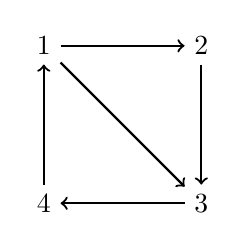
\begin{tikzpicture}
\node (atom1) at (0,2) {1};
\node (atom2) at (2,2) {2};
\node (atom3) at (2,0) {3};
\node (atom4) at (0,0) {4};
\draw[->, thick] (atom1)--(atom2);
\draw[->, thick] (atom2)--(atom3);
\draw[->, thick] (atom3)--(atom4);
\draw[->, thick] (atom4)--(atom1);
\draw[->, thick] (atom1) -- (atom3);
\end{tikzpicture}
\end{center}
This would be suitable to characterize an interpretation whose domain is the first four positive whole numbers, and which interprets $Rxy$ as being true of and only of:
	\begin{center}
		\ntuple{1, 2},
		\ntuple{2, 3},
		\ntuple{3, 4},
		\ntuple{4, 1},
		\ntuple{1, 3}
	\end{center}
Equally we might offer:

\begin{center}
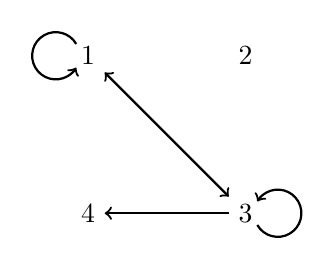
\begin{tikzpicture}
\node (atom1) at (0,2) {1};
\node (atom2) at (2,2) {2};
\node (atom3) at (2,0) {3};
\node (atom4) at (0,0) {4};
\draw[->, thick] (atom3)--(atom4);
\draw[->, thick] (atom1)+(-0.15,0.15) arc (-330:-30:.3);
\draw[->, thick] (atom3)+(0.15,-0.15) arc (-150:150:.3);
\draw[<->, thick] (atom1) -- (atom3);
\end{tikzpicture}
\end{center}
for an interpretation with the same domain, which interprets $Rxy$ as being true of and only of:
	\begin{center}
		\ntuple{1, 3},
		\ntuple{3, 1},
		\ntuple{3, 4},
		\ntuple{1, 1},
		\ntuple{3, 3}
	\end{center}
If we wanted, we could make our diagrams more complex. For example, we could add names as labels for particular objects. Equally, to symbolize the extension of a one-place predicate, we might simply draw a ring around some particular objects and stipulate that the thus encircled objects (and only them) are to fall under the predicate $Hx$, say.


\chapter{Truth in FOL}\label{s:TruthFOL}
We know what interpretations are. Since, among other things, they tell us which predicates are true of which objects, they will provide us with an account of the truth of atomic sentences. However, we must also present a detailed account of what it is for an arbitrary FOL sentence to be true or false in an interpretation.

But we defined what a sentence was by first specifying what a formula is. Formulas like $Hx$ aren't the sorts of things that are true or false in interpretations. Only sentences are true or false. But if we provide extra information we can determine the truth of $Hx$: we need to specify what $x$ refers to. This is done by using a variable assignment: \factoidbox{A variable assignment specifies an object for each variable.}

We define whether a formula is true or false \emph{under a variable assignment}.
We know from \S\ref{s:FOLSentences} that there are three kinds of formulas in FOL:
	\begin{ebullet}
		\item atomic formulas
		\item formulas whose main logical operator is a sentential connective
		\item formulas whose main logical operator is a quantifier
	\end{ebullet}
We need to explain truth for all three kinds of formula.

We will provide a completely general explanation in this section. However, to try to keep the explanation comprehensible, we will, at several points, use the following interpretation:
	\begin{ekey}
		\item[\text{domain}] all people born before 2000\textsc{ce}
		\item[a] Aristotle
		\item[b] Beyonc\'e
		\item[Px] \gap{x} is a philosopher
		\item[Rxy] \gap{x} was born before \gap{y}
	\end{ekey}
This will be our \emph{go-to example} in what follows.

\section{Atomic formulas}
Atomic formulas are things like $Px$, $Pb$ or $Rax$.

An atomic sentence like $Pb$ is checked for truth just by consulting our interpretation: $Px$ is `\gap{x} is a philosopher', so if we're looking at $Pb$ we fill out the gap with  Beyonc\'e, and  Beyonc\'e is not a philosopher, so $Pb$ is false.

What about $Px$? This reads something like `they are a philosopher'. The question is who `they' refers to, or in the logic terms: who $x$ is. This depends on a variable assignment. Our variable assignment needs to give an object in our domain for the variable $x$. For example, it might give Beyonc\'e, then since Beyonc\'e is not a philosopher, $Px$ would be false on this variable assignment. Our variable assignment doesn't need to specify one of the objects that are named, it can give us anyone in our domain, e.g.~Queen Elizabeth II. Under the variable assignment which assigns $x$ Queen Elizabeth II, $Px$ is false: Queen Elizabeth II is not a philosopher.

%The truth of atomic \emph{sentences} should be fairly straightforward. The sentence $Pa$ should be true just in case $Px$ is true of $a$. Given our go-to interpretation, this is true iff Aristotle is a philosopher. Aristotle is a philosopher. So the sentence is true. Equally, $Pb$ is false on our go-to interpretation.

Likewise, on this interpretation, $Rab$ is true iff the object named by $a$ was born before the object named by $b$. Well, Aristotle was born before Beyonc\'e. So $Rab$ is true. Equally, $Raa$ is false: Aristotle was not born before Aristotle. How about $Rax$? Well what does our variable assignment specify for $x$? If we have a variable assignment where $x$ is Queen Elizabeth II, then $Rax$ is true: Aristotle was born before Queen Elizabeth II.

Dealing with atomic sentences, then, is very intuitive. When \meta{R} is an $n$-place predicate and $\metaterm_1,\,\metaterm_2\ldots\metaterm_{n}$ are names or variables, then

	\factoidbox{
		$\meta{R}\metaterm_1\metaterm_2\ldots\metaterm_{n}$ is true in an interpretation under a variable assignment \textbf{iff}\\
		$\meta{R}$ is true of the objects referred to by $\metaterm_{1}, \metaterm_{2}, \ldots, \metaterm_{n}$ in that interpretation under that variable assignment (considered in that order)
	}



\section{Sentential connectives}
We saw in \S\ref{s:FOLSentences} that FOL formulas can be built up from simpler ones using the truth-functional connectives that were familiar from TFL. The rules governing these truth-functional connectives are \emph{exactly} the same as they were when we considered TFL. Here they are:
	\factoidbox{
		$\metaX \eand \metaY$ is true in an interpretation under a variable assignment \textbf{iff}\\ both $\metaX$ and $\metaY$ is true in that interpretation under that variable assignment

		\
		\\
		$\metaX \eor \metaY$ is true in an interpretation under a variable assignment \textbf{iff}\\ either $\metaX$ is true or $\metaY$ is true in that interpretation under that variable assignment

		\
		\\$\enot \metaX$ is true in an interpretation under a variable assignment \textbf{iff} \\$\metaX$ is false in that interpretation under that variable assignment

		\
		\\$\metaX \eif \metaY$ is true in an interpretation under a variable assignment \textbf{iff}\\ either $\metaX$ is false or $\metaY$ is true in that interpretation under that variable assignment

		%\
		%\\$\metaX \eiff \metaY$ is true in an interpretation under a variable assignment \textbf{iff} \\$\metaX$ has the same truth value as $\metaY$ in that interpretation under that variable assignment
	}
This is just another presentation of the truth rules we gave for the connectives in TFL; it just does so in a slightly different way. Some examples will probably help to illustrate the idea. On our go-to interpretation:
	\begin{earg}
		\item[\textbullet] $ Pa$ is true
		\item[\textbullet] $Rab \eand Pb$ is false because, although $Rab$ is true, $Pb$ is false
		\item[\textbullet] $\enot Pa$ is false
		\item[\textbullet] $Pa \eand \enot(Pb\eand Rab)$ is true, because $Pa$ is true and $Pb$ is false, so $Pb\eand Rab$ is false, thus $\enot (Pb\eand Rab)$ is also true.
	\end{earg}
Make sure you understand these examples.

We can also carry variable assignments around with us. Consider a variable assignment which assigns David Hume to $x$. Then \begin{ebullet}
\item $Px$ is true under this variable assignment: David Hume was a philosopher
\item $Bxa$ is false under this variable assignment: David Hume was born after Aristotle
\item $Px\eif Bxa$ is false under this variable assignment: $Px$ is true and $Bxa$ is false, so by our rule for $\eif$, $Px\eif Bxa$ is false.
\end{ebullet}


\section{When the main logical operator is a quantifier}
The exciting innovation in FOL, though, is the use of \emph{quantifiers}.

Consider the following interpretation:
\begin{center}
\begin{tikzpicture}
\node (A) [alice,monitor,sword,minimum size=1cm] {Alice};
\node (B)[bob,evil,sword,minimum size=1cm,right=1cm of A] {Bob};
\node[charlie,monitor,female, minimum size=1cm,below=.8cm of A] {Cathy};
\node[businessman,minimum size=1cm,skin=brown,below=.8cm of B] {Denny};
\end{tikzpicture}

\begin{ekey}\item[\text{domain}] People in above picture (Alice, Bob, Cathy and Denny)
\item[Hx] \gap{x} has horns (Bob)
\item[Sx] \gap{x} carrying a sword (Alice and Bob)
\item[Cx]\gap{x} is looking at a computer (Alice and Cathy)
%\item[Gx] nothing
\end{ekey}
\end{center}

Is $\exists x Sx$ true? To check this we see if there is a choice of an object for $x$ which gives us a variable assignment under which $Sx$ is true. Consider assigning Alice to $x$, which we can as shorthand write by $x\mapsto \text{Alice}$. Under this variable assignment, $Sx$ is true: Alice does have a sword. So $\exists x Sx$ is true. There is a choice of an object in our domain for $x$ under which $Sx$ is true.

What about $\forall x Sx$? This is true iff $Sx$ is true under any choice of a person for $x$. Let's go through them. \begin{center}
\begin{tabular}{l|c}
&$Sx$\Bstrut\\\hline\Tstrut
$x\mapsto\text{Alice}$&T\\
$x\mapsto \text{Bob}$&T\\
$x\mapsto \text{Cathy}$&F\\
$x\mapsto \text{Denny}$&F
\end{tabular}
\end{center}So $\forall x Sx$ is false: it is not the case that $Sx$ is true under any choice of an object for $x$: when we have an assignment of Cathy to $x$, $Sx$ is false.

What about $\forall x(Sx\eif (Hx\eor Cx))$
\begin{center}
\begin{tabular}{l|ccccc}
&$Sx$&$Hx$&$Cx$&$Hx\eor Cx$&$Sx\eif (Hx\eor Cx)$\Bstrut\\\hline\Tstrut
$x\mapsto\text{Alice}$&T&F&T&T&T\\
$x\mapsto \text{Bob}$&T&T&F&T&T\\
$x\mapsto \text{Cathy}$&F&F&T&T&T\\
$x\mapsto \text{Denny}$&F&F&F&F&T
\end{tabular}
\end{center}
So $Sx\eif (Hx\eor Cx)$  is true under every assignment of an object to the variable $x$. And so $\forall x(Sx\eif (Hx\eor Cx))$ is true.



We have to tread more carefully once we start having multiple quantifiers. Let's walk through some cases.

Consider a new interpretation: \begin{center}
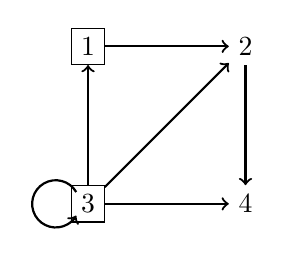
\begin{tikzpicture}
\node (atom1) [draw] at (0,2) {1};
\node (atom2) at (2,2) {2};
\node (atom3) [draw] at (0,0) {3};
\node (atom4)  at (2,0) {4};
\draw[->, thick] (atom3)+(-0.15,0.15) arc (-330:-30:.3);
\draw[<-, thick] (atom2) -- (atom3);
\draw[<-,thick] (atom1)--(atom3);
\draw[<-, thick] (atom4)--(atom3);
\draw[->, thick] (atom1)--(atom2);
\draw[->, thick] (atom2)--(atom4);
\end{tikzpicture}

 \begin{ekey}
\item[\text{domain}] Numbers 1, 2, 3 and 4.
\item[Rxy] There is an arrow from \gap{x} to \gap{y} in the diagram.
\item[Sx] There is a square around \gap{x} in the diagram.
\end{ekey}
\end{center}

 Is $\exists x\forall y Rxy$ true? We need to find some choice of an object for $x$ where $\forall y Rxy$ is true under that choice (``variable assignment''). Let's (with foresight) chose the number 3 for $x$ ($x\mapsto 3$). Let's call this particular variable assignment $\alpha$. $\alpha$ also assigns objects to all other variables of the language (we just don't care which ones) Is $\forall y Rxy$ true under the variable assignment $\alpha$? Intuitively, the answer is yes as there is an arrow from 3 to 1, 2, 3, and 4, that is, all objects of the domain.
 
  %To check this we need to do something more with our variable assignment: we need to extend it with a choice of an object for $y$. 
 To evaluate the universal quantifier $\forall y$ we need to think about all ways of picking an object for $y$, not only the one of the particular variable assignment $\alpha$. Moreover, in doing so we need to keep the assignment of $3$ to $x$ fixed. This means we need to evaluate whether $Rxy$ is true under all assignments that differ from the assignment $\alpha$ at most in that they might assign a different object $y$ than $\alpha$. Since in this case our domain has four objects this means that there are only four different objects an assignment can assign to $x$ (whilst assigning $3$ to $x$). If $Rxy$ is true on all these options $\exists x\forall y Rxy$ is true:
\begin{center}
 \begin{tabular}{cc|c}
&&$Rxy$\Bstrut\\\hline\Tstrut
$x\mapsto 3$&$y\mapsto 1$&T\\
$x\mapsto 3$&$y\mapsto 2$&T\\
$x\mapsto 3$&$y\mapsto 3$&T\\
$x\mapsto 3$&$y\mapsto 4$&T\\
 \end{tabular}
\end{center}So under every variable assignment that differs from $\alpha$ at most at $y$ (it assigns the same object as $\alpha$ to a variable except for $y$ to which it may assign a different object)  $Rxy$ true. This tells us that $\forall y Rxy$ is true under the variable assignment $\alpha$ for which $x\mapsto 3$. And \emph{that} tells us that $\exists x\forall y Rxy$ is true: there's an assignment of the variable $x$ under which the constituent formula $\forall y Rxy$ is true.

What about $\exists x \exists y(Rxy \eand Ryx)$? To show that it is true we will want to choose an object that we can assign to $x$ under which $\exists y (Rxy\eand Ryx)$ is true. Let's consider $x\mapsto 3$ (again I'm using my forsight of what will come to choose carefully). Now is $\exists y (Rxy\eand Ryx)$  true under the variable assignment $x\mapsto 3$? We need to find an extension of this which chooses an object for $y$ under which $Rxy\eand Ryx$ is true. Consider $y\mapsto 3$. We now have a variable assignment $x\mapsto 3, y\mapsto 3$. They are different variables but there's nothing stopping them denoting the same object. And we can then consider whether $Rxy\eand Ryx$ is true under this interpretation. Well, $Rxy$ is true: 3 does have an arrow to 3. And $Ryx$ is also true: 3 does have an arrow to 3. So by our clause for $\eand$, $Rxy\eand Ryx$ is true under this variable assignment $x\mapsto 3, y\mapsto 3$. And so $\exists y(Rxy\eand Ryx)$ is true under the variable assignment $x\mapsto 3$. And so $\exists x\exists y(Rxy\eand Ryx)$ is true in this interpretation.

One more example: $\forall x(Sx\eif \exists y Rxy)$? To check this is true we will need to go through each of our objects for $x$ and see that $Sx\eif \exists y Rxy$ is true under that interpretation. We can already see if $Sx$ is true under each variable assignment, and if we find that $Sx$ is false that's enough information to determine that $Sx\eif \exists y Rxy$ is true (check the definition of truth for $\eif$ to see this):
\begin{center}
\begin{tabular}{c|ccc}
&$Sx$&$\exists y Rxy$&$Sx\eif\exists y Rxy$\Bstrut\\\hline\Tstrut
$x\mapsto 1$&T&?&?\\
$x\mapsto 2$&F&?&T\\
$x\mapsto 3$&T&?&?\\
$x\mapsto 4$&F&?&T
\end{tabular}
\end{center}

So we need to check  whether $\exists y Rxy$ is true under the variable assignments $x\mapsto 1$ and $x\mapsto 3$.

Consider $x\mapsto 1$. We can find an object for $y$ where $Rxy$ is true under that variable assignment: consider $y\mapsto 2$. Since there is an arrow from 1 to 2, $Rxy$ is true in the variable assignment $x\mapsto 1$ and $y\mapsto 2$. Thus $\exists y Rxy$ is true on the variable assignment $x\mapsto 1$. We're also able to do something similar for $x\mapsto 3$:
\begin{center}
\begin{tabular}{cc|c}
&&$Rxy$\Bstrut\\\hline\Tstrut
$x\mapsto 1$&$y\mapsto 2$&T\\
$x\mapsto 3$&$y\mapsto 3$&T
 \end{tabular}
\end{center}So we now have
\begin{center}
\begin{tabular}{c|ccc}
&$Sx$&$\exists y Rxy$&$Sx\eif\exists y Rxy$\Bstrut\\\hline\Tstrut
$x\mapsto 1$&T&T&T\\
$x\mapsto 2$&F&?&T\\
$x\mapsto 3$&T&T&T\\
$x\mapsto 4$&F&?&T
\end{tabular}
\end{center}So $\forall x(Sx\eif \exists y Rxy)$ is true. Informally we might say this as: for every number that has a square around it has an arrow going out of it.

One final example: $\forall x\forall y Rxy$. To check this we will need to consider all choices for $x$ and all choices for $y$ and check $Rxy$ is true on all of them. There are 16 such choices. But we won't have to go through them all: it'll be false. Consider $x\mapsto 1$ and $y\mapsto 4$. $Rxy$ is false under this variable assignment: there is no arrow from 1 to 4. Thus $\forall yRxy$ is false on the variable assignment $x\mapsto 1$. And so $\forall x\forall y Rxy$ is false in the interpretation.

 Let's now give a formal definition of the idea we've been using here. Quantified formulas like $\exists y Rxy$ still need to be given truth conditions \emph{relative to a variable assignment}, because we'll need to specify an assignment of an object for the free variable $x$. So we define when $\exists \metav\metaX$ is true under a variable assignment $\alpha$, which might be, e.g.~$x\mapsto 1$. To give a general definition, though we might also consider whether $\forall y Rxy$ is true under a variable assignment $x\mapsto 1, y\mapsto 4$. This is slightly odd: we're considering $\exists y Rxy$ but have been told who $y$ refers to already. However when we evaluate it we simply ignore whatever our given variable assignment tells us about $y$: we consider variable assignments that modify the assignment by changing what is assigned to $y$. And by modifying it to $x\mapsto 1, y\mapsto2$ we have a variable assignment under which $Rxy$ is true, so $\exists y Rxy$ is true under the original variable assignment $x\mapsto 1, y\mapsto 4$.

 Similarly consider $\exists x Sx$ under the variable assignment $x\mapsto 1$. To evaluate this we consider modification of this variable assignment which assign other objects to $x$. Under the variable assignment $x\mapsto 2$, $Sx$ is true.  So under our original variable assignment $\exists x Sx$ is true: it didn't matter what our original variable assignment was, we ignored this and considered variants to evaluate its truth.

 This is a general feature: Sentences, which have all variables bound, have truth values independent of any variable assignment they're evaluated with: when we have a quantifier like $\exists x$ or $\forall x$ we ignore whatever our original variable assignment told us about $x$. So when all our variables are bound by quantifiers, all the original components of our variable assignment are ignored. To summarise: Sentences are simply true or false in interpretations, variable assignments don't matter.

 Now for our formal definition:
\factoidbox{
$\forall \metav\metaX$ is true under a variable assignment $\alpha$\\
\textbf{iff} $\metaX$ is true under \emph{every} variable assignment $\beta$ that differs from $\alpha$ at most in $\metav$.

\bigskip

$\exists \metav\metaX$ is true under a variable assignment $\alpha$\\
\textbf{iff} $\metaX$ is true under \emph{some} variable assignment $\beta$ that differs from $\alpha$ at most in $\metav$.
}
To be clear: all this is doing is formalizing the intuitive idea expressed in our examples. The result is a bit ugly, and the final definition might look a bit opaque. Hopefully, though, the \emph{spirit} of the idea is clear.


%\section{When the main logical operator is a quantifier}
%The exciting innovation in FOL, though, is the use of \emph{quantifiers}.
%%When is $\forall x Px$ true? The thought is: we introduce a new name: $d$, and we check if $Pd$ is true in the various interpretations where $d$ names the different objects.
%But expressing the truth conditions for quantified sentences is a bit more fiddly than one might first expect.
%
%Here is a na\"{i}ve first thought. We want to say that $\forall x Fx$ is true iff $Fx$ is true of everything in the domain. This should not be too problematic: our interpretation will specify directly what $Fx$ is true of.
%
%Unfortunately, this na\"{i}ve thought is not general enough. For example, we want to be able to say that $\forall x \exists y Lxy$ is true just in case $\exists y Lxy$ is true of everything in the domain. This is problematic, since our interpretation does not directly specify what $\exists y Lxy$ is to be true of. Instead, whether or not this is true of something should follow just from the interpretation of $Lxy$, the domain, and the meanings of the quantifiers.
%
%So here is a second na\"{i}ve thought. We might try to say that $\forall x \exists y Lxy$ is to be true in an interpretation iff $\exists y L\meta{a}y$ is true for \emph{every} name \meta{a} that we have included in our interpretation. Similarly, we might try to say that $\exists y L\meta{a}y$ is true just in case $L\meta{a}\meta{b}$ is true for \emph{some} name \meta{b} that we have included in our interpretation.
%
%Unfortunately, this is not right either. To see this, observe that in our go-to interpretation, we have only given interpretations for \emph{two} names, $a$ and $b$, but the domain---all people born before the year 2000\textsc{ce}---contains many more than two people. We have no intention of trying to name \emph{all} of them!
%
%So here is a third thought. (And this thought is not na\"{i}ve, but correct.) Although it is not the case that we have named \emph{everyone}, each person \emph{could} have been given a name. So we should focus on this possibility of extending an interpretation, by adding a new name. We will offer a few examples of how this might work, centring on our go-to interpretation, and we will then present the formal definition.
%
%In our go-to interpretation, $\exists x Rbx$ should be true. After all, in the domain, there is certainly someone who was born after Beyonc\'e. Lady Gaga is one of those people. Indeed, if we were to extend our go-to interpretation---temporarily, mind---by adding the name $c$ to refer to Lady Gaga, then $Rbc$ would be true on this extended interpretation. This, surely, should suffice to make $\exists x Rbx$ true on the original go-to interpretation.
%
%In our go-to interpretation, $\exists x (Px \eand Rxa)$ should also be true. After all, in the domain, there is certainly someone who was both a philosopher and born before Aristotle. Socrates is one such person. Indeed, if we were to extend our go-to interpretation by letting a new name, $c$, denote Socrates, then $Wc \eand Rca$ would be true on this extended interpretation. Again, this should surely suffice to make $\exists x (Px \eand Rxa)$ true on the original go-to interpretation.
%
%In our go-to interpretation, $\forall x \exists y Rxy$ should be false. After all, consider the last person born in the year 1999. We don't know who that was, but if we were to extend our go-to interpretation by letting a new name, $d$, denote that person, then we would not be able to find anyone else in the domain to denote with some further new name, perhaps $e$, in such a way that $Rde$ would be true. Indeed, no matter \emph{whom} we named with $e$, $Rde$ would be false. This observation is surely sufficient to make $\exists y Rdy$ \emph{false} in our extended interpretation, which in turn is surely sufficient to make $\forall x \exists y Rxy$ false on the original go-to interpretation.
%
%If you have understood these three examples, good. That's what matters. Strictly speaking, though, we still need to give a precise definition of the truth conditions for quantified sentences. The result, sadly, is a bit ugly, and requires a few new definitions. Brace yourself!
%
%Suppose that \metaX is an expression with that $\meta{x}$ is free in $\metaX$ (i.e.~no quantifiers $\forall\meta{x}$ or $\exists\meta{x}$ already). We will write this thus:
%$$\metaX(\ldots \meta{x} \ldots \meta{x} \ldots)$$
%Suppose also that \meta{c} is a name. Then we will write:
%$$\metaX(\ldots \meta{c} \ldots \meta{c} \ldots)$$
%for the formula obtained by replacing every occurrence of $\meta{x}$ in \metaX with $\meta{c}$. The resulting formula is called a \define{substitution instance} of $\forall \meta{x}\metaX$ and $\exists\meta{x}\metaX$.  $\meta{c}$ is called the \define{instantiating name}. So:
%	$$\exists x (Rex \eiff Fx)$$
%is a substitution instance of
%	$$\forall y \exists x (Ryx \eiff Fx)$$
%with the instantiating name $e$.
%
%\newglossaryentry{substitution instance}{
%  name = substitution instance,
%  description = {the result of replacing every occurrence of a {free variable} in a {formula} with a \gls{name}}
%}
%
%Armed with this notation, the rough idea is as follows. The sentence $\forall \meta{x}\metaX(\ldots \meta{x} \ldots \meta{x} \ldots)$ will be true iff $\metaX(\ldots \meta{c} \ldots \meta{c}\ldots)$ is true no matter what object (in the domain) we name with $\meta{c}$. Similarly, the sentence $\exists \meta{x}\metaX$ will be true iff there is \emph{some} way to assign the name $\meta{c}$ to an object that makes $\metaX(\ldots \meta{c} \ldots \meta{c} \ldots)$ true. More precisely, we stipulate:
%	\factoidbox{
%		$\forall \meta{x}\metaX(\ldots \meta{x}\ldots\meta{x}\ldots)$ is true in an interpretation \textbf{iff}\\
%		$\metaX(\ldots \meta{c} \ldots \meta{c}\ldots)$ is true in \emph{every} interpretation that extends the original interpretation by assigning an object to any name $\meta{c}$ (without changing the interpretation in any other way).
%
%		\
%		\\
%		$\exists \meta{x}\metaX(\ldots \meta{x}\ldots\meta{x}\ldots)$ is true in an interpretation \textbf{iff}\\
%		$\metaX(\ldots \meta{c}\ldots\meta{c}\ldots)$ is true in \emph{some} interpretation that extends the original interpretation by assigning an object to some name $\meta{c}$ (without changing the interpretation in any other way).
%	}
%To be clear: all this is doing is formalizing (very pedantically) the intuitive idea expressed on the previous page. The result is a bit ugly, and the final definition might look a bit opaque. Hopefully, though, the \emph{spirit} of the idea is clear.


\begin{practiceproblems}
\problempart
\label{pr.TorF1}
Consider the following interpretation:
	\begin{ebullet}
		\item The domain comprises only Corwin and Benedict
		\item `$\atom{A}{x}$' is to be true of both Corwin and Benedict
		\item `$\atom{B}{x}$' is to be true of Benedict only
		\item `$\atom{N}{x}$' is to be true of no one
		\item `$c$' is to refer to Corwin
	\end{ebullet}
Determine whether each of the following sentences is true or false in that interpretation:
\begin{earg}
\item $\atom{B}{c}$ \hfill \myanswer{False}
\item $\atom{A}{c} \eiff \enot \atom{N}{c}$ \hfill \myanswer{True}
\item $\atom{N}{c} \eif (\atom{A}{c} \eor \atom{B}{c})$ \hfill \myanswer{True}
\item $\forall x\,\atom{A}{x}$ \hfill \myanswer{True}
\item $\forall x \enot \atom{B}{x}$ \hfill \myanswer{False}
\item $\exists x(\atom{A}{x} \eand \atom{B}{x})$ \hfill \myanswer{True}
\item $\exists x(\atom{A}{x} \eif \atom{N}{x})$ \hfill \myanswer{False}
\item $\forall x(\atom{N}{x} \eor \enot \atom{N}{x})$ \hfill \myanswer{True}
\item $\exists x\,\atom{B}{x} \eif \forall x\,\atom{A}{x}$ \hfill \myanswer{True}
\end{earg}

\problempart
\label{pr.TorF2}
Consider the following interpretation:	
	\begin{ebullet}
		\item The domain comprises only Lemmy, Courtney and Eddy
		\item `$\atom{G}{x}$' is to be true of Lemmy, Courtney and Eddy.
		\item `$\atom{H}{x}$' is to be true of and only of Courtney
		\item `$\atom{M}{x}$' is to be true of and only of Lemmy and Eddy
		\item `$c$' is to refer to Courtney
		\item `$e$' is to refer to Eddy
	\end{ebullet}
Determine whether each of the following sentences is true or false in that interpretation:
\begin{earg}
\item $\atom{H}{c}$ \hfill \myanswer{True}
\item $\atom{H}{e}$\hfill \myanswer{False}
\item $\atom{M}{c} \eor \atom{M}{e}$ \hfill \myanswer{True}
\item $\atom{G}{c} \eor \enot \atom{G}{c}$ \hfill \myanswer{True}
\item $\atom{M}{c} \eif \atom{G}{c}$ \hfill \myanswer{True}
\item $\exists x\,\atom{H}{x}$ \hfill \myanswer{True}
\item $\forall x\,\atom{H}{x}$ \hfill \myanswer{False}
\item $\exists x \enot \atom{M}{x}$ \hfill \myanswer{True}
\item $\exists x(\atom{H}{x} \eand \atom{G}{x})$ \hfill \myanswer{True}
\item $\exists x(\atom{M}{x} \eand \atom{G}{x})$ \hfill \myanswer{True}
\item $\forall x(\atom{H}{x} \eor \atom{M}{x})$ \hfill \myanswer{True}
\item $\exists x\,\atom{H}{x} \eand \exists x\,\atom{M}{x}$ \hfill \myanswer{True}
\item $\forall x(\atom{H}{x} \eiff \enot \atom{M}{x})$ \hfill \myanswer{True}
\item $\exists x\,\atom{G}{x} \eand \exists x \enot \atom{G}{x}$ \hfill \myanswer{False}
\item $\forall x\exists y(\atom{G}{x} \eand \atom{H}{y})$ \hfill \myanswer{True}
\end{earg}

\problempart
\label{pr.TorF3}
Following the diagram conventions introduced at the end of \S23, consider the following interpretation:	
\begin{center}
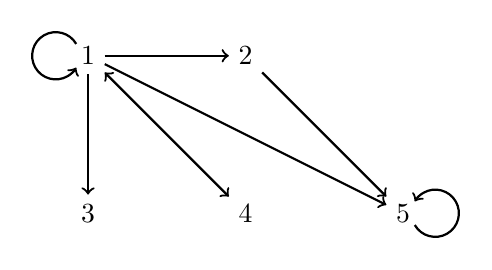
\begin{tikzpicture}
\node (atom1) at (0,2) {1};
\node (atom2) at (2,2) {2};
\node (atom4) at (0,0) {3};
\node (atom5) at (2,0) {4};
\node (atom6) at (4,0) {5};
\draw[->, thick] (atom1)+(-0.15,0.15) arc (-330:-30:.3); 
\draw[->, thick] (atom6)+(0.15,-0.15) arc (-150:150:.3); 
\draw[->, thick] (atom1) -- (atom2);
\draw[->, thick] (atom1) -- (atom4);
\draw[<->, thick] (atom1) -- (atom5);
\draw[->, thick] (atom1) -- (atom6);
\draw[->, thick] (atom2) -- (atom6);
\end{tikzpicture}
\end{center}
Determine whether each of the following sentences is true or false in that interpretation:
\begin{earg}
\item $\exists x\,\atom{R}{x,x}$ \hfill \myanswer{True}
\item $\forall x\,\atom{R}{x,x}$ \hfill \myanswer{False}
\item $\exists x \forall y\,\atom{R}{x,y}$ \hfill \myanswer{True}
\item $\exists x \forall y\,\atom{R}{y,x}$ \hfill \myanswer{False}
\item $\forall x \forall y \forall z ((\atom{R}{x,y} \eand \atom{R}{y,z}) \eif \atom{R}{x,z})$ \hfill \myanswer{False}
\item $\forall x \forall y \forall z ((\atom{R}{x,y} \eand \atom{R}{x,z}) \eif \atom{R}{y,z})$ \hfill \myanswer{False}
\item $\exists x \forall y \enot \atom{R}{x,y}$ \hfill \myanswer{True}
\item $\forall x(\exists y\,\atom{R}{x,y} \eif \exists y\,\atom{R}{y,x})$ \hfill \myanswer{True}
\item $\exists x \exists y (\enot x = y \eand \atom{R}{x,y} \eand \atom{R}{y,x})$ \hfill \myanswer{True}
\item $\exists x \forall y(\atom{R}{x,y} \eiff x = y)$ \hfill \myanswer{True}
\item $\exists x \forall y(\atom{R}{y,x} \eiff x = y)$ \hfill \myanswer{False}
\item $\exists x \exists y(\enot x = y \eand \atom{R}{x,y} \eand \forall z(\atom{R}{z,x} \eiff y = z))$ \hfill \myanswer{True}
\end{earg}
\end{practiceproblems}

\chapter{Semantic concepts}

Offering a precise definition of truth in FOL was more than a little fiddly, but now that we are done, we can define various central logical notions. These will look very similar to the definitions we offered for TFL. However, remember that they concern \emph{interpretations}, rather than valuations.

%We will use the symbol $\entails$ for FOL much as we did for TFL. So:
\factoidbox{
	$$\metaX_1, \metaX_2, \ldots, \metaX_n \therefore\metaZ$$ is \define{valid}
iff there is no interpretation in which all of $\metaX_1, \metaX_2, \ldots, \metaX_n$ are true and in which \metaZ is false. }
%Derivatively,
%	$$\entails\metaX$$
%means that \metaX is true in every interpretation.

The other logical notions also have corresponding definitions in FOL:
\factoidbox{
\begin{itemize}
\item An FOL sentence $\metaX$ is a \define{logical truth} iff $\metaX$ is true in every interpretation.%; i.e.,  $\entails\metaX$.
\newglossaryentry{logical truth}
{
name=logical truth,
description={A \gls{sentence of FOL} that is true in every \gls{interpretation}. Note that the equivalent notion for TFL is `tautology'}
}

\item $\metaX$ is a \define{contradiction} iff $\metaX$ is false in every interpretation.%; i.e., $\entails\enot\metaX$.
\newglossaryentry{contradiction of FOL}
{
  name=contradiction (of FOL),
  text=contradiction,
description={A \gls{sentence of FOL} that is false in every \gls{interpretation}}
}

%\item $\metaX_1, \metaX_2, \ldots \metaX_n \therefore \metaZ$ is \define{valid in FOL} iff there is no interpretation in which all of the premises are true and the conclusion is false; i.e., $\metaX_1,\metaX_2,\ldots \metaX_n \entails\metaZ$. It is \define{invalid in FOL} otherwise.
%\newglossaryentry{logically valid in FOL}
%{
%  name=logical validity (in FOL),
%  text = logically valid,
%description={A property held by arguments if and only if no \gls{interpretation} makes all premises true and the conclusion false}
%}

\item Two FOL sentences \metaX and \metaY are \define{logically equivalent} iff they are true in exactly the same interpretations as each other.%r; i.e., both $\metaX\entails\metaY$ and $\metaY\entails\metaX$.

\newglossaryentry{logically equivalent in FOL}
{
  name=logical equivalence (in FOL),
  text = logically equivalent,
description={A property held by pairs of \glspl{sentence of FOL} if and only if the sentences have the same truth value in every \gls{interpretation}.}
}

\item The FOL sentences $\metaX_1,\metaX_2,\ldots, \metaX_n$ are \define{jointly logically consistent} iff there is some interpretation in which all of the sentences are true. They are \define{jointly logically inconsistent} iff there is no such interpretation.
\newglossaryentry{logically consistent in FOL}
{
  name=logical consistency (in FOL),
  text=jointly consistent,
description={A property held by \glspl{sentence of FOL} if and only if some \gls{interpretation} makes all the sentences true}
}
\end{itemize}
}

\chapter{Using interpretations}
\label{sec.UsingModels}

\section{Logical truths and contradictions}
Suppose we want to show that $\exists xAxx \eif Bd$ is \emph{not} a logical truth. This requires showing that the sentence is not true in every interpretation; i.e.,\ that it is false in some interpretation. If we can provide just one interpretation in which the sentence is false, then we will have shown that the sentence is not a logical truth.

In order for $\exists xAxx \eif Bd$ to be false, the antecedent ($\exists x Axx$) must be true, and the consequent ($Bd$) must be false. To construct such an interpretation, we start by specifying a domain. Keeping the domain small makes it easier to specify what the predicates will be true of, so we will start with a domain that has just one member. For concreteness, let's say it is the city of Paris.
	\begin{ekey}
		\item[\text{domain}] Paris
	\end{ekey}
The name $d$ must refer to something in the domain, so we have no option but:
	\begin{ekey}
		\item[d] Paris
	\end{ekey}
Recall that we want $\exists x Axx$ to be true, so we want all members of the domain to be paired with themselves in the extension of $A$. We can just offer:
	\begin{ekey}
		\item[Axy] \gap{x} is identical with \gap{y}
	\end{ekey}
Now $Add$ is true, so it is surely true that $\exists x Axx$. Next, we want $Bd$ to be false, so the referent of $d$ must not be in the extension of $B$. We might simply offer:
	\begin{ekey}
		\item[Bx] \gap{x} is in Germany
	\end{ekey}
Now we have an interpretation where $\exists x Axx$ is true, but where $Bd$ is false. So there is an interpretation where $\exists x Axx \eif Bd$ is false. So $\exists x Axx \eif Bd$ is not a logical truth.

We can just as easily show that $\exists xAxx \eif Bd$ is not a contradiction. We need only specify an interpretation in which $\exists xAxx \eif Bd$ is true; i.e., an interpretation in which either $\exists x Axx$ is false or $Bd$ is true. Here is one:
	\begin{ekey}
		\item[\text{domain}] Paris
		\item[d] Paris
		\item[Axy] \gap{x} is identical with \gap{y}
		\item[Bx] \gap{x} is in France
	\end{ekey}
This shows that there is an interpretation where $\exists xAxx \eif Bd$ is true. So $\exists x Axx \eif Bd$ is not a contradiction.

\section{Logical equivalence}
Suppose we want to show that $\forall x Sx$ and $\exists x Sx$ are not logically equivalent. We need to construct an interpretation in which the two sentences have different truth values; we want one of them to be true and the other to be false. We start by specifying a domain. Again, we make the domain small so that we can specify extensions easily. In this case, we will need at least two objects. (If we chose a domain with only one member, the two sentences would end up with the same truth value. In order to see why, try constructing some partial interpretations with one-member domains.) For concreteness, let's take:
	\begin{ekey}
		\item[\text{domain}] Ornette Coleman, Miles Davis
	\end{ekey}
We can make $\exists x Sx$ true by including something in the extension of $S$, and we can make $\forall x Sx$ false by leaving something out of the extension of $S$. For concreteness we will offer:
	\begin{ekey}
		\item[Sx] \gap{x} plays saxophone
	\end{ekey}
Now $\exists x Sx$ is true, because $Sx$ is true of Ornette Coleman. Slightly more precisely, extend our interpretation by allowing $c$ to name Ornette Coleman.  $Sc$ is true in this extended interpretation, so $\exists x Sx$ was true in the original interpretation. Similarly, $\forall x Sx$ is false, because $Sx$ is false of Miles Davis. Slightly more precisely, extend our interpretation by allowing $d$ to name Miles Davis, and $Sd$ is false in this extended interpretation, so $\forall x Sx$ was false in the original interpretation. We have provided a counter-interpretation to the claim that $\forall x Sx$ and $\exists x Sx$ are logically equivalent.
	\factoidbox{
		To show that $\metaX$ is not a logical truth, it suffices to find an interpretation where $\metaX$ is false.

		To show that $\metaX$ is not a contradiction, it suffices to find an interpretation where $\metaX$ is true.

		To show that $\metaX$ and $\metaY$ are not logically equivalent, it suffices to find an interpretation where one is true and the other is false.
	}

\section{Validity, entailment and consistency}
To test for validity, entailment, or consistency, we typically need to produce interpretations that determine the truth value of several sentences simultaneously.

Consider the following argument in FOL:
$$\exists x(Gx \eif Ga) \therefore \exists x Gx \eif Ga$$
To show that this is invalid, we must make the premise true and the conclusion false. The conclusion is a conditional, so to make it false, the antecedent must be true and the consequent must be false. Clearly, our domain must contain two objects. Let's try:
	\begin{ekey}
		\item[\text{domain}] Karl Marx, Ludwig von Mises
		\item[Gx] \gap{x} hated communism
		\item[a] Karl Marx
	\end{ekey}
Given that Marx wrote \emph{The Communist Manifesto}, $Ga$ is plainly false in this interpretation. But von Mises famously hated communism, so $\exists x Gx$ is true in this interpretation. Hence $\exists x Gx \eif Ga$ is false, as required.

Does this interpretation make the premise true? Yes it does! Note that $Ga \eif Ga$ is true. (Indeed, it is a logical truth.) But then certainly $\exists x (Gx \eif Ga)$ is true, so the premise is true, and the conclusion is false, in this interpretation. The argument is therefore invalid.

In passing, note that we have also shown that $\exists x(Gx \eif Ga)$ does \emph{not} entail $\exists x Gx \eif Ga$. Equally, we have shown that the sentences $\exists x (Gx \eif Ga)$ and $\enot (\exists x Gx \eif Ga)$ are jointly consistent.

Let's consider a second example. Consider:
	$$\forall x \exists y Lxy \therefore \exists y \forall x Lxy$$
Again, we want to show that this is invalid. To do this, we must make the premises true and the conclusion false. Here is a suggestion:
	\begin{ekey}
		\item[\text{domain}] UK citizens currently in a civil partnership with another UK citizen
		\item[Lxy] \gap{x} is in a civil partnership with \gap{y}
	\end{ekey}
The premise is clearly true on this interpretation. Anyone in the domain is a UK citizen in a civil partnership with some other UK citizen. That other citizen will also, then, be in the domain. So for everyone in the domain, there will be someone (else) in the domain with whom they are in a civil partnership. Hence $\forall x \exists y Lxy$ is true. However, the conclusion is clearly false, for that would require that there is some single person who is in a civil partnership with everyone in the domain, and there is no such person, so the argument is invalid. We observe immediately that the sentences $\forall x \exists y Lxy$ and $\enot\exists y \forall x Lxy$ are jointly consistent and that $\forall x \exists y Lxy$ does not entail $\exists y \forall x Lxy$.

For our third example, we'll mix things up a bit. In \S\ref{s:Interpretations}, we described how we can present some interpretations using diagrams. For example:
\begin{center}
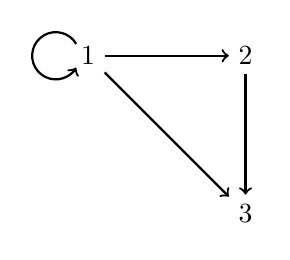
\begin{tikzpicture}
\node (atom1) at (0,2) {1};
\node (atom2) at (2,2) {2};
\node (atom3) at (2,0) {3};
\draw[->, thick] (atom1)--(atom2);
\draw[->, thick] (atom1)--(atom3);
\draw[->, thick] (atom1)+(-0.15,0.15) arc (-330:-30:.3);
\draw[->, thick] (atom2) -- (atom3);
\end{tikzpicture}
\end{center}
Using the conventions employed in \S\ref{s:Interpretations}, the domain of this interpretation is the first three positive whole numbers, and $Rxy$ is true of x and y just in case there is an arrow from x to y in our diagram. Here are some sentences that the interpretation makes true:
	\begin{ebullet}
		\item $\forall x \exists y Ryx$
		\item $\exists x \forall y Rxy$ \hfill witness 1
		\item $\exists x \forall y (Ryx \eiff x = y)$ \hfill witness 1
		\item $\exists x \exists y \exists z ((\enot y = z \eand Rxy) \eand Rzx)$ \hfill witness 2
		\item $\exists x \forall y \enot Rxy$ \hfill witness 3
		\item $\exists x (\exists y Ryx \eand \enot \exists y Rxy)$ \hfill witness 3
	\end{ebullet}
This immediately shows that all of the preceding six sentences are jointly consistent. We can use this observation to generate \emph{invalid} arguments, e.g.:
	\begin{align*}
		\forall x \exists y Ryx, \exists x \forall y Rxy  &\therefore  \forall x \exists y Rxy\\
		\exists x \forall y Rxy, \exists x \forall y \enot Rxy & \therefore \enot \exists x \exists y \exists z (\enot y = z \eand (Rxy \eand Rzx))
	\end{align*}
and many more besides.

	\factoidbox{
	To show that $\metaX_1, \metaX_2, \ldots, \metaX_n \therefore \metaZ$ is invalid, it suffices to find an interpretation where all of $\metaX_1, \metaX_2, \ldots, \metaX_n$ are true and where $\metaZ$ is false.

	That same interpretation will show that $\metaX_1, \metaX_2, \ldots, \metaX_n$ do not entail $\metaZ$.

	It will also show that $\metaX_1, \metaX_2, \ldots, \metaX_n, \enot \metaZ$ are jointly consistent.}
When you provide an interpretation to refute a claim---to logical truth, say, or to entailment---this is sometimes called providing a \emph{counter-interpretation} (or providing a \emph{counter-model}).

\begin{practiceproblems}
\problempart
\label{pr.Contingent}
Show that each of the following is neither a validity nor a contradiction:
\begin{earg}
\item $\atom{D}{a} \eand \atom{D}{b}$

\myanswer{The sentence is true in this model:
\begin{ekey}
	\item[\text{domain}] Stan
	\item[D(x)] Stan
	\item[a] Stan
	\item[b] Stan
\end{ekey}
And it is false in this model:
\begin{ekey}
	\item[\text{domain}] Stan
	\item[D(x)] % $\emptyset$
	\item[a] Stan
	\item[b] Stan
\end{ekey}}
\item \leftsolutions\ $\exists x\,\atom{T}{x,h}$

\myanswer{The sentence is true in this model:
\begin{ekey}
	\item[\text{domain}] Stan
	\item[T(x,y)] \ntuple{Stan, Stan}
	\item[h] Stan
\end{ekey}
And it is false in this model:
\begin{ekey}
	\item[\text{domain}] Stan
	\item[T(x,y)] % $\emptyset$
	\item[h] Stan
\end{ekey}}

\item $\atom{P}{m} \eand \enot\forall x\,\atom{P}{x}$

\myanswer{	The sentence is true in this model:
\begin{ekey}
	\item[\text{domain}] Stan, Ollie
	\item[P(x)] Stan
	\item[m] Stan
\end{ekey}
And it is false in this model:
\begin{ekey}
	\item[\text{domain}] Stan
	\item[P(x)] % $\emptyset$
	\item[m] Stan
\end{ekey}}
\item $\forall z\, \atom{J}{z} \eiff \exists y\,\atom{J}{y}$
\item $\forall x (\atom{W}{x,m,n} \eor \exists y\atom{L}{x,y})$
\item $\exists x (\atom{G}{x} \eif \forall y\,\atom{M}{y})$
\item $\exists x (x = h \eand x = i)$
\end{earg}

\solutions
\problempart
\label{pr.NotEquiv}
Show that the following pairs of sentences are not logically equivalent.
\begin{earg}
\item $\atom{J}{a}$, $\atom{K}{a}$

\myanswer{Making the first sentence true and the second false:
\begin{ekey}
	\item[\text{domain}] $0$
	\item[J(x)] $0$
	\item[K(x)] % $\emptyset$
	\item[a] $0$
\end{ekey}}
\item $\exists x\,\atom{J}{x}$, $\atom{J}{m}$

\myanswer{Making the first sentence true and the second false:
\begin{ekey}
	\item[\text{domain}] $0$, $1$
	\item[J(x)] $0$
	\item[m] $1$
\end{ekey}}
\item $\forall x\,\atom{R}{x,x}$, $\exists x\,\atom{R}{x,x}$

\myanswer{Making the first sentence false and the second true:
\begin{ekey}
	\item[\text{domain}] $0$, $1$
	\item[R(x,y)] \ntuple{$0$,$0$}
\end{ekey}}
\item $\exists x\,\atom{P}{x} \eif \atom{Q}{c}$, $\exists x (\atom{P}{x} \eif \atom{Q}{c})$

\myanswer{Making the first sentence false and the second true:
\begin{ekey}
	\item[\text{domain}] $0$, $1$
	\item[P(x)] $0$
	\item[Q(x)] % $\emptyset$
	\item[c] $0$
\end{ekey}}
\item $\forall x(\atom{P}{x} \eif \enot \atom{Q}{x})$, $\exists x(\atom{P}{x} \eand \enot \atom{Q}{x})$

\myanswer{Making the first sentence true and the second false:
\begin{ekey}
	\item[\text{domain}] $0$
	\item[P(x)] % $\emptyset$
	\item[Q(x)] % $\emptyset$
\end{ekey}}
\item $\exists x(\atom{P}{x} \eand \atom{Q}{x})$, $\exists x(\atom{P}{x} \eif \atom{Q}{x})$

\myanswer{Making the first sentence false and the second true:
\begin{ekey}
	\item[\text{domain}] $0$
	\item[P(x)] % $\emptyset$
	\item[Q(x)] $0$
\end{ekey}}
\item $\forall x(\atom{P}{x}\eif \atom{Q}{x})$, $\forall x(\atom{P}{x} \eand \atom{Q}{x})$

\myanswer{Making the first sentence true and the second false:
\begin{ekey}
	\item[\text{domain}] $0$
	\item[P(x)] % $\emptyset$
	\item[Q(x)] $0$
\end{ekey}}
\item $\forall x\exists y\,\atom{R}{x,y}$, $\exists x\forall y\,\atom{R}{x,y}$

\myanswer{Making the first sentence true and the second false:
\begin{ekey}
	\item[\text{domain}] $0$, $1$
	\item[R(x,y)] \ntuple{$0$, $1$}, \ntuple{$1$, $0$}
\end{ekey}}
\item $\forall x\exists y\,\atom{R}{x,y}$, $\forall x\exists y\,\atom{R}{y,x}$

\myanswer{Making the first sentence false and the second true:
\begin{ekey}
	\item[\text{domain}] $0$, $1$
	\item[R(x,y)] \ntuple{$0$, $0$}, \ntuple{$0$, $1$}
\end{ekey}}
\end{earg}


\problempart
Show that the following sentences are jointly satisfiable:
\begin{earg}
\item $\atom{M}{a}, \enot \atom{N}{a}, Pa, \enot \atom{Q}{a}$
\item $\atom{L}{e,e}, \atom{L}{e,g}, \enot \atom{L}{g,e}, \enot \atom{L}{g,g}$
\item $\enot (\atom{M}{a} \eand \exists x\,\atom{A}{x}), Ma \eor \atom{F}{a}, \forall x(\atom{F}{x} \eif \atom{A}{x})$
\item $\atom{M}{a} \eor \atom{M}{b}, \atom{M}{a} \eif \forall x \enot \atom{M}{x}$
\item $\forall y\,\atom{G}{y}, \forall x (\atom{G}{x} \eif \atom{H}{x}), \exists y \enot \atom{I}{y}$
\item $\exists x(\atom{B}{x} \eor \atom{A}{x}), \forall x \enot \atom{C}{x}, \forall x\bigl[(\atom{A}{x} \eand \atom{B}{x}) \eif Cx\bigr]$
\item $\exists x\,\atom{X}{x}, \exists x\,\atom{Y}{x}, \forall x(\atom{X}{x} \eiff \enot \atom{Y}{x})$
\item $\forall x(\atom{P}{x} \eor \atom{Q}{x}), \exists x\enot(\atom{Q}{x} \eand \atom{P}{x})$
\item $\exists z(\atom{N}{z} \eand \atom{O}{z,z}), \forall x\forall y(\atom{O}{x,y} \eif \atom{O}{y,x})$
\item $\enot \exists x \forall y\,\atom{R}{x,y}, \forall x \exists y\,\atom{R}{x,y}$
\item $\enot \atom{R}{a,a}$, $\forall x (x=a \eor \atom{R}{x,a})$

\myanswer{The sentences are both true in this interpretation:
\begin{ekey}
	\item[\text{domain}] Harry, Sally
	\item[R(x,y)]\ntuple{Sally, Harry}
	\item[a] Harry
	\end{ekey}}
\item $\forall x\forall y\forall z[(x=y \eor y=z )\eor x=z]$, $\exists x\exists y\ \enot x= y$

\myanswer{There are no predicates or constants, so we only need to give a domain.
Any domain with 2 elements will do.}
\item $\exists x\exists y((\atom{Z}{x} \eand \atom{Z}{y} )\eand x=y)$, $\enot \atom{Z}{d}$, $d=e$
\end{earg}

\problempart
Show that the following arguments are invalid:
\begin{earg}
\item $\forall x(\atom{A}{x} \eif \atom{B}{x}) \therefore \exists x\,\atom{B}{x}$
\item $\forall x(\atom{R}{x} \eif \atom{D}{x}), \forall x(\atom{R}{x} \eif \atom{F}{x}) \therefore \exists x(\atom{D}{x} \eand \atom{F}{x})$
\item $\exists x(\atom{P}{x}\eif \atom{Q}{x}) \therefore \exists x\,\atom{P}{x}$
\item $\atom{N}{a} \eand \atom{N}{b} \eand \atom{N}{c} \therefore \forall x\,\atom{N}{x}$
\item $\atom{R}{d,e}, \exists x\,\atom{R}{xd} \therefore \atom{R}{e,d}$
\item $\exists x(\atom{E}{x} \eand \atom{F}{x}), \exists x\,\atom{F}{x} \eif \exists x\,\atom{G}{x} \therefore \exists x(\atom{E}{x} \eand \atom{G}{x})$
\item $\forall x\,\atom{O}{x,c}, \forall x\,\atom{O}{c,x} \therefore \forall x\,\atom{O}{x,x}$
\item $\exists x(\atom{J}{x} \eand \atom{K}{x}), \exists x \enot \atom{K}{x}, \exists x \enot \atom{J}{x} \therefore \exists x(\enot \atom{J}{x} \eand \enot \atom{K}{x})$
\item $\atom{L}{a,b} \eif \forall x\,\atom{L}{x,b}, \exists x\,\atom{L}{x,b} \therefore \atom{L}{b,b}$
\item $\forall x(\atom{D}{x} \eif \exists y\,\atom{T}{y,x}) \therefore \exists y \exists z\ \enot y= z$
\end{earg}


\end{practiceproblems}


\chapter{Reasoning about all interpretations}

\section{Logical truths and contradictions}
We can show that a sentence is \emph{not} a logical truth just by providing one carefully specified interpretation: an interpretation in which the sentence is false. To show that something is a logical truth, on the other hand, it would not be enough to construct ten, one hundred, or even a thousand interpretations in which the sentence is true. A sentence is only a logical truth if it is true in \emph{every} interpretation, and there are infinitely many interpretations. We need to reason about all of them, and we cannot do this by dealing with them one by one!

Sometimes, we can reason about all interpretations fairly easily. For example, we can offer a relatively simple argument that $Raa\eiff Raa$ is a logical truth:
	\begin{quote}
		\label{allmodels1}
		Any relevant interpretation will give $Raa$ a truth value. If $Raa$ is true in an interpretation, then $Raa \eiff Raa$ is true in that interpretation. If $Raa$ is false in an interpretation, then $Raa \eiff Raa$ is true in that interpretation. These are the only alternatives. So $Raa \eiff Raa$ is true in every interpretation. Therefore, it is a logical truth.
	\end{quote}
This argument is valid, of course, and its conclusion is true. However, it is not an argument in FOL. Rather, it is an argument in English \emph{about} FOL: it is an argument in the metalanguage.

Note another feature of the argument. Since the sentence in question contained no quantifiers, we did not need to think about how to interpret $a$ and $R$; the point was just that, however we interpreted them, $Raa$ would have some truth value or other. (We could ultimately have given the same argument concerning TFL sentences.)

Here is another bit of reasoning. Consider the sentence $\forall x(Rxx\eiff Rxx)$. Again, it should obviously be a logical truth, but to say precisely why is quite a challenge. We cannot say that $Rxx \eiff Rxx$ is true in every interpretation, since $Rxx \eiff Rxx$ is not even a \emph{sentence} of FOL (remember that $x$ is a variable, not a name). So we have to be a bit cleverer.
	\begin{quote}
		Consider some arbitrary interpretation. Consider some arbitrary member of the domain, which, for convenience, we will call \emph{obbie}, and suppose we extend our original interpretation by adding a new name, $c$, to name \emph{obbie}. Then either $Rcc$ will be true or it will be false. If $Rcc$ is true, then $Rcc \eiff Rcc$ is true. If $Rcc$ is false, then $Rcc \eiff Rcc$ will be true. So either way, $Rcc \eiff Rcc$ is true. Since there was nothing special about \emph{obbie}---we might have chosen any object---we see that no matter how we extend our original interpretation by allowing $c$ to name some new object, $Rcc \eiff Rcc$ will be true in the new interpretation. So $\forall x (Rxx \eiff Rxx)$ was true in the original interpretation. But we chose our interpretation arbitrarily, so $\forall x (Rxx \eiff Rxx)$ is true in every interpretation. It is therefore a logical truth.
	\end{quote}
This is quite longwinded, but, as things stand, there is no alternative. In order to show that a sentence is a logical truth, we must reason about \emph{all} interpretations.

\section{Other cases}
Similar points hold of other cases too. Thus, we must reason about all interpretations if we want to show:
	\begin{ebullet}
		\item that a sentence is a contradiction; for this requires that it is false in \emph{every} interpretation.
		\item that two sentences are logically equivalent; for this requires that they have the same truth value in \emph{every} interpretation.
		\item that some sentences are jointly inconsistent; for this requires that there is no interpretation in which all of those sentences are true together; i.e.\ that, in \emph{every} interpretation, at  least one of those sentences is false.
		\item that an argument is valid; for this requires that the conclusion is true in \emph{every} interpretation where the premises are true.
		\item that some sentences entail another sentence.
	\end{ebullet}
The problem is that, with the tools available to you so far, reasoning about all interpretations is a serious challenge! Let's take just one more example. Here is an argument which is obviously valid:
	$$\forall x(Hx \eand Jx) \therefore \forall x Hx$$
After all, if everything is both H and J, then everything is H. But we can only show that the argument is valid by considering what must be true in every interpretation in which the premise is true. To show this, we would have to reason as follows:
	\begin{quote}
		Consider an arbitrary interpretation in which the premise $\forall x(Hx \eand Jx)$ is true. It follows that, however we expand the interpretation with a new name, for example $c$, $Hc \eand Jc$ will be true in this new interpretation. $Hc$ will, then, also be true in this new interpretation. But since this held for \emph{any} way of expanding the interpretation, it must be that $\forall x Hx$ is true in the old interpretation. We've assumed nothing about the interpretation except that it was one in which $\forall x(Hx \eand Jx)$  is true, so any interpretation in which $\forall x(Hx \eand Jx)$ is true is one in which $\forall x Hx$ is true. The argument is valid!
\end{quote}
Even for a simple argument like this one, the reasoning is somewhat complicated. For longer arguments, the reasoning can be extremely torturous.

The following table summarises whether a single (counter-)interpretation suffices, or whether we must reason about all interpretations.


\begin{center}
\begin{tabular}{l l l}
%\cline{2-3}
 & \textbf{Yes} & \textbf{No}\\
 \hline
%\cline{2-3}
logical truth? & all interpretations & one counter-interpretation\\
contradiction? &  all interpretations  & one counter-interpretation\\
equivalent? & all interpretations & one counter-interpretation\\
consistent? & one interpretation & all interpretations\\
valid? & all interpretations & one counter-interpretation\\
entailment? & all interpretations & one counter-interpretation\\
\end{tabular}
\end{center}
\label{table.ModelOrArgument}

This might usefully be compared with the table at the end of \S\ref{s:PartialTruthTable}. The key difference resides in the fact that TFL concerns truth tables, whereas FOL concerns interpretations. This difference is deeply important, since each truth-table only ever has finitely many lines, so that a complete truth table is a relatively tractable object. By contrast, there are infinitely many interpretations for any given sentence(s), so that reasoning about all interpretations can be a deeply tricky business.

%!TEX root = forallxbris.tex
\part{Natural deduction for FOL}
\label{ch.NDFOL}
\addtocontents{toc}{\protect\mbox{}\protect\hrulefill\par}


\chapter{Basic rules for FOL}\label{s:BasicFOL}

FOL makes use of all of the connectives of TFL. So proofs in FOL will use all of the basic and derived rules from Part~\ref{ch.NDTFL}. We will also use the proof-theoretic notions (particularly, the symbol `$\proves$') introduced there. However, we will also need some new basic rules to govern the quantifiers.


\section{Universal elimination}Consider:
\begin{earg}
\prem Everyone is happy
\conc Catrin is happy.
\end{earg} This is a valid argument. Generally, then, from the claim that everything is F, you can infer that any particular thing is F. You name it; it's F. So the following should be fine:
\begin{fitchproof}
	\hypo{a}{\forall xFx}
	\have{c}{Fa} \Ae{a}
\end{fitchproof}
We obtained line 2 by dropping the universal quantifier and replacing `$x$' with `$a$'.

This isn't restricted to simple properties. Consider the following argument:
\begin{earg}
\prem Every cat is sleeping.
\conc If Fluffy is a cat, then she is sleeping.
\end{earg}
This is a valid argument. And it will be allowed by our rule $\forall$E:
\begin{fitchproof}
	\hypo{a}{\forall x(Cx\eif Sx)}
	\have{c}{Cf\eif Sf} \Ae{a}
\end{fitchproof}
Note here that we have to replace two instances of `$x$' with our name: `$f$' or Fluffy. Indeed it would have been fine to do with any name. We can even do it with names we already have. Consider the following:
\begin{earg}
\prem Pavel owes everyone money.
\conc Pavel owes himself money.
\end{earg}
We we symbolise this as:
\begin{earg}
\prem $\forall x Opx$
\conc $Opp$
\end{earg}
This is valid: the premise says \emph{everything} in the domain owes money to Pavel; and Pavel is something in the domain. So it implies that Pavel owes money to himself.

%A closely related sentence is: \begin{earg}
%\item Pavel owes money to everyone \emph{else}.
%\end{earg}and that will not be symbolised as $\forall x Oxx$; however, we do not yet have the resources to symbolise at. In \S\ref{ch.identity} we will introduce identity which will allow us to formalise it properly.

This argument is also directly allowed by our rule $\forall$E:
\begin{fitchproof}
	\hypo{a}{\forall xOpx}
	\have{c}{Opp} \Ae{a}
\end{fitchproof}

We can now give our general rule: whenever you have a sentence $\forall \meta{x}\metaX(\ldots \meta{x} \ldots\meta{x}\ldots)$, for example $\forall x Fx$, $\forall x (Cx\eif Sx)$, $\forall x Opx$; one can conclude that we have the sentence which is obtained by stripping of the quantifier and replacing every free occurrence of the variable by a name, be it $a,b,c\ldots$. So we could derive $Fa$, $Cf\eif Sf$ or $Opp$.

%We obtained line 2 by dropping the universal quantifier and replacing every instance of `$x$' with `$a$'. Equally, the following should be allowed:
%\begin{fitchproof}
%	\hypo{a}{\forall xRxxd}
%	\have{c}{Rddd} \Ae{a}
%\end{fitchproof}
%We obtained line 2 here by dropping the universal quantifier and replacing every instance of `$x$' with `$d$'. We could have done the same with any other name we wanted.

Here is the formal specification of the universal elimination rule ($\forall$E):
\factoidbox{
\begin{fitchproof}
	\have[m]{a}{\forall \meta{x}\metaX(\ldots \meta{x} \ldots \meta{x}\ldots)}
	\have[\ ]{c}{\metaX(\ldots \meta{c} \ldots \meta{c}\ldots)} \Ae{a}
\end{fitchproof}}
The point is that you can obtain any \emph{substitution instance} of a universally quantified formula: \textbf{replace every instance of the quantified variable with any name you like}. (Of course, you need to replace every free occurrence of $x$ in $X$ by the same name.)

I should emphasize that (as with every elimination rule) you can only apply the $\forall$E rule when the universal quantifier is the main logical operator. Thus the following is outright banned:
\begin{fitchproof}
	\hypo{a}{\forall x Bx \eif Bk}
	\have{c}{Bb \eif Bk}\by{naughtily attempting to invoke $\forall$E}{a}
\end{fitchproof}
This is illegitimate, since `$\forall x$' is not the main logical operator in line 1. (If you need a reminder as to why this sort of inference should be banned, reread \S\ref{s:MoreMonadic}.)

\section{Existential introduction}
The following argument is valid:
\begin{earg}
\prem Catrin is happy
\conc Someone is happy.
\end{earg}

This is the idea of our existential introduction rule: from the claim that some particular thing is F, you can infer that something is F:
\begin{fitchproof}
	\hypo{a}{Fa}
	\have{c}{\exists x Fx} \existsI{a}
\end{fitchproof}
We obtained line 2 by replacing the name `$a$' with the variable `$x$' and adding $\exists x$ in front of the sentence. This will be permissible by our rule of $\exists$I.

This isn't restricted to simple properties.
\begin{earg}
\prem Bob is a money and knows sign language.
\conc There is a monkey who knows sign language.
\end{earg}
\begin{fitchproof}
	\hypo{a}{Mb\eand Sb}
	\have{c}{\exists x (Mx\eand Sx)} \existsI{a}
\end{fitchproof}

Or even
\begin{earg}
\prem Catrin is friends with someone who is friends with everyone.
\conc Someone is friends with someone who is friends with everyone.
\end{earg}
\begin{fitchproof}
	\hypo{a}{\exists x (Fcx\eand\forall y Fxy)}
	\have{c}{\exists z\exists x(Fzx\eand \forall y Fxy)} \existsI{a}
\end{fitchproof}We replaced the name, `$c$' with the variable `$z$' and added $\exists z$ at the beginning of the sentence.


This rule will now allow us to carefully work through our brain teaser from \S\ref{s:orE}
\label{s:ExistsE}

\begin{quote}
Three people are standing in a row looking at eachother.
\begin{center}
\begin{tikzpicture}[people/.style={minimum width=1.5cm}]
\node[people, alice] (alice) {Alice};
\node[people, bob, right=of alice] (bob) {Bob};
\node[people, charlie, right=of bob] (charlie) {Charlie};
\end{tikzpicture}
\end{center}
Alice is happy. Charlie is not happy. Is there someone who is happy who is looking at someone who is not happy?
\end{quote}  Answer: Yes.

We can formalise this argument as: $$Lab,\;Lbc,\;Ha,\;\enot Hc\;\therefore\;\exists x\exists y(Hx\eand (Lxy\eand\enot Hx)).$$ And we can show it is valid. In \S\ref{s:orE} we wrote this in a pseudo-formal style.
\begin{fitchproof}
	\have{lem}{\text{Bob is either happy or he's not happy}}\LEM
	\open
	\hypo{b}{\text{Suppose Bob is happy}}
	\have{ab}{\text{Then happy Bob is looking at unhappy Charlie}}
	\have{abc}{\text{So someone who is happy is looking at someone who is not happy.}}
	\close
	\open
	\hypo{b2}{\text{Suppose Bob is unhappy}}
	\have{ab2}{\text{Then happy Alice is looking at unhappy Bob}}
	\have{abc2}{\text{So someone who is happy is looking at someone who is not happy.}}
	\close
	\have{con}{\text{Therefore, someone who is happy is looking at someone who is not happy.}}\orE{lem,b-abc,b2-abc2}
\end{fitchproof}

We can now fill out the details of this to see that it's a formal proof:
\begin{fitchproof}
\hypo{1}{Lab}
\hypo{2}{Lbc}
\hypo{3}{Ha}
\hypo{4}{\enot Hc}
	\have{lem}{Hb\eor\enot Hb}\LEM
	\open
	\hypo{b}{Hb}
	\have{a}{Lbc\eand\enot Hc}\andI{2,b}
	\have{ab}{Hb\eand (Lbc\eand\enot Hc)}\andI{a,b}
		\have{ab2}{\exists y(Hb\eand (Lby\eand\enot Hy))}\existsI{ab}
		\have{abc}{\exists x\exists y(Hx\eand (Lxy\eand\enot Hx))}\existsI{ab2}
	\close
	\open
	\hypo{b2}{\enot Hb}
		\have{a}{Lab\eand\enot Hb}\andI{b2,1}
	\have{ab2}{Ha\eand (Lab\eand\enot Hb)}\andI{3,a}
		\have{ab22}{\exists y(Ha\eand (Lay\eand\enot Hy))}\existsI{ab2}
		\have{abc2}{\exists x\exists y(Hx\eand (Lxy\eand\enot Hx))}\existsI{ab22}
	\close
			\have{con}{\exists x\exists y(Hx\eand Lxy\eand\enot Hx)}\orE{lem,b-abc,b2-abc2}
\end{fitchproof}

\bigskip
Consider the following example:
\begin{earg}
\prem Narcissus loves himeself.
\conc There is someone who loves Narcissus.
\end{earg}This is a valid argument. The formalised version, which will be allowed by our rule is:
\begin{fitchproof}
	\hypo{a}{Lnn}
	\have{c}{\exists x Lxn} \existsI{a}
\end{fitchproof} This shows us that we do not have to replace \emph{all} instances of the name with the variable. Though of course we can if we wish: we could also deduce there is someone who loves himself.

To give our rule in general we need to introduce some new notation for this ability to replace just some of our instances of the name: If $\metaX$ is a sentence containing the name $\meta{c}$, we can emphasize this by writing `$\metaX(\ldots \meta{c} \ldots \meta{c}\ldots)$'. \textbf{We will write `$\metaX(\ldots \meta{x} \ldots \meta{c}\ldots)$' to indicate any formula obtained by replacing \emph{some or all} of the instances of the name \meta{c} with the variable \meta{x}}. Armed with this, our introduction rule is:
\factoidbox{
\begin{fitchproof}
	\have[m]{a}{\metaX(\ldots \meta{c} \ldots \meta{c}\ldots)}
	\have[\ ]{c}{\exists \meta{x}\metaX(\ldots \meta{x} \ldots \meta{c}\ldots)} \Ei{a}
\end{fitchproof}
\meta{x} must not occur in $\metaX(\ldots \meta{c} \ldots \meta{c}\ldots)$
}All the cases we've seen in this section follow this rule.

You might have noticed the additional constraint that's added to the rule. It is {part} of the rule; so if you are asked to write the rule $\exists$I  you {must} include this constraint. However, you will not need to worry about it in practice. It's simply there to guarantee that applications of the rule yield sentences of FOL. If the rule were not there we would be allowed to argue as follows:
\begin{fitchproof}
	\hypo{a}{\exists xLnx}
	\have{e}{\exists x \exists x Lxx}\by{naughtily attempting to invoke $\exists$I}{a}
\end{fitchproof}But this expression on line 2 contains clashing variables. It will not count as a sentence of FOL.


\section{Empty domains}
The following proof combines our two new rules for quantifiers:
	\begin{fitchproof}
		\hypo{a}{\forall x Fx}
		\have{in}{Fa}\Ae{a}
		\have{e}{\exists x Fx}\Ei{in}
	\end{fitchproof}
Could this be a bad proof? If anything exists at all, then certainly we can infer that something is F, from the fact that everything is F. But what if \emph{nothing} exists at all? Then it is surely vacuously true that everything is F; however, it does not following that something is F, for there is nothing to \emph{be} F. So if we claim that, as a matter of logic alone, `$\exists x Fx$' follows from `$\forall x Fx$', then we are claiming that, as a matter of \emph{logic alone}, there is something rather than nothing. This might strike us as a bit odd.

Actually, we are already committed to this oddity. In \S\ref{s:FOLBuildingBlocks}, we stipulated that domains in FOL must have at least one member. We then defined a logical truth (of FOL) as a sentence which is true in every interpretation. Since `$\exists x(Ax\eor\enot Ax)$' will be true in every interpretation, this \emph{also} had the effect of stipulating that it is a matter of logic that there is something rather than nothing.

Since it is far from clear that logic should tell us that there must be something rather than nothing, we might well be cheating a bit here.

If we refuse to cheat, though, then we pay a high cost. Here are three things that we want to hold on to:
	\begin{ebullet}
		\item $\forall x Fx \proves Fa$: after all, that was $\forall$E.
		\item $Fa \proves \exists x Fx$: after all, that was $\exists$I.
		\item the ability to copy-and-paste proofs together: after all, reasoning works by putting lots of little steps together into rather big chains.
	\end{ebullet}
If we get what we want on all three counts, then we have to countenance that $\forall xFx \proves \exists x Fx$. So, if we get what we want on all three counts, the proof system alone tells us that there is something rather than nothing. And if we refuse to accept that, then we have to surrender one of the three things that we want to hold on to!

Before we start thinking about which to surrender, we might want to ask how \emph{much} of a cheat this is. Granted, it may make it harder to engage in theological debates about why there is something rather than nothing. But the rest of the time, we will get along just fine. So maybe we should just regard our proof system (and FOL, more generally) as having a very slightly limited purview. If we ever want to allow for the possibility of \emph{nothing}, then we will have to cast around for a more complicated proof system. But for as long as we are content to ignore that possibility, our proof system is perfectly in order. (As, similarly, is the stipulation that every domain must contain at least one object.)


\section{Universal introduction}
Suppose you had shown of each particular thing that it is F (and that there are no other things to consider). Then you would be justified in claiming that everything is F. This would motivate the following proof rule. If you had established each and every single substitution instance of `$\forall x Fx$', then you can infer `$\forall x Fx$'.

Unfortunately, that rule would be utterly unusable. To establish each and every single substitution instance would require proving `$Fa$', `$Fb$', $\ldots$, `$Fj_2$', $\ldots$, `$Fr_{79002}$', $\ldots$, and so on. Indeed, since there are infinitely many names in FOL, this process would never come to an end. So we could never apply that rule. We need to be a bit more cunning in coming up with our rule for introducing universal quantification.

Our cunning thought will be inspired by considering:
$$\forall x Fx \therefore\ \forall y Fy$$
This argument should \emph{obviously} be valid. After all, alphabetical variation ought to be a matter of taste, and of no logical consequence. But how might our proof system reflect this? Suppose we begin a proof thus:
\begin{fitchproof}
	\hypo{x}{\forall x Fx}
	\have{a}{Fa} \Ae{x}
\end{fitchproof}
We have proved `$Fa$'. And, of course, nothing stops us from using the same justification to prove `$Fb$', `$Fc$', $\ldots$, `$Fj_2$', $\ldots$, `$Fr_{79002}, \ldots$, and so on until we run out of space, time, or patience. But reflecting on this, we see that there is a way to prove $F\meta{c}$, for any name \meta{c}. And if we can do it for \emph{any} thing, we should surely be able to say that `$F$' is true of \emph{everything}. This therefore justifies us in inferring `$\forall y Fy$', thus:
\begin{fitchproof}
	\hypo{x}{\forall x Fx}
	\have{a}{Fa} \Ae{x}
	\have{y}{\forall y Fy} \Ai{a}
\end{fitchproof}
The crucial thought here is that `$a$' was just some \emph{arbitrary} name. There was nothing special about it---we might have chosen any other name---and still the proof would be fine. And this crucial thought motivates the universal introduction rule ($\forall$I):
\factoidbox{
\begin{fitchproof}
	\have[m]{a}{\metaX(\ldots \meta{c} \ldots \meta{c}\ldots)}
	\have[\ ]{c}{\forall \meta{x}\metaX(\ldots \meta{x} \ldots \meta{x}\ldots)} \Ai{a}
\end{fitchproof}
	\meta{c} must not occur in any undischarged assumption or premise.\\
	\meta{x} must not occur in $\metaX(\ldots \meta{c} \ldots \meta{c}\ldots)$
	}
It is important to appreciate that to apply the rule correctly \textbf{we must replace every occurrence of the name $c$ by the variable $x$}. A crucial aspect of this rule, though, is bound up in the first constraint. This constraint ensures that we are always reasoning at a sufficiently general level (the second constraint guarantees that the variable $x$ is not already bound by a different quantifier in $X$ which would lead to unintended results.) 
%\footnote{Recall from \S\ref{s:BasicTFL} that we are treating `$\ered$' as a canonical contradiction. But if it were the canonical contradiction as involving some \emph{constant}, it might interfere with the constraint mentioned here. To avoid such problems, we will treat `$\ered$' as a canonical contradiction \emph{that involves no particular names}.}

To see the constraint in action, consider this terrible argument:
	\begin{quote}
		Everyone loves Kylie Minogue; therefore everyone loves themselves.
	\end{quote}
We might symbolize this obviously invalid inference pattern as:
$$\forall x Lxk \therefore \forall x Lxx$$
Now, suppose we tried to offer a proof that vindicates this argument:
\begin{fitchproof}
	\hypo{x}{\forall x Lxk}
	\have{a}{Lkk} \Ae{x}
	\have{y}{\forall x Lxx} \by{naughtily attempting to invoke $\forall$I}{a}
\end{fitchproof}\noindent
This is not allowed, because `$k$' occurred already in an undischarged assumption, namely, on line 1. The crucial point is that, if we have made any assumptions about the object we are working with, then we are not reasoning generally enough to license $\forall$I.

Although the name may not occur in any \emph{undischarged} assumption, it may occur as a discharged assumption. That is, it may occur in a subproof that we have already closed. For example:
\begin{fitchproof}
	\open
		\hypo{f1}{Gd}
		\have{f2}{Gd}\by{R}{f1}
	\close
	\have{ff}{Gd \eif Gd}\ci{f1-f2}
	\have{zz}{\forall z(Gz \eif Gz)}\Ai{ff}
\end{fitchproof}
This tells us that `$\forall z (Gz \eif Gz)$' is a \emph{theorem}. And that is as it should be.

\section{Existential elimination}
Suppose we know that \emph{something} is F. The problem is that simply knowing this does not tell us which thing is F. So it would seem that from `$\exists x Fx$' we cannot immediately conclude `$Fa$', `$Fe_{23}$', or any other substitution instance of the sentence. What can we do?

Suppose we know that something is F, and that everything which is F is G. In (almost) natural English, we might reason thus:
	\begin{quote}
		Since something is F, there is some particular thing which is an F. We do not know anything about it, other than that it's an F, but for convenience, let's call it `obbie'. So: obbie is F. Since everything which is F is G, it follows that obbie is G. But since obbie is G, it follows that something is G. And nothing depended on which object, exactly, obbie was. So, something is G.
	\end{quote}
We might try to capture this reasoning pattern in a proof as follows:
\begin{fitchproof}
	\hypo{es}{\exists x Fx}
	\hypo{ast}{\forall x(Fx \eif Gx)}
	\open
		\hypo{s}{Fo}
		\have{st}{Fo \eif Go}\Ae{ast}
		\have{t}{Go} \ce{st, s}
		\have{et1}{\exists x Gx}\Ei{t}
	\close
	\have{et2}{\exists x Gx}\Ee{es,s-et1}
\end{fitchproof}\noindent
Breaking this down: we started by writing down our assumptions. At line 3, we made an additional assumption: `$Fo$'. This was just a substitution instance of `$\exists x Fx$'. On this assumption, we established `$\exists x Gx$'. Note that we had made no \emph{special} assumptions about the object named by `$o$'; we had \emph{only} assumed that it satisfies `$Fx$'. So nothing depends upon which object it is. And line 1 told us that \emph{something} satisfies `$Fx$', so our reasoning pattern was perfectly general. We can discharge the specific assumption `$Fo$', and simply infer `$\exists x Gx$' on its own.

Putting this together, we obtain the existential elimination rule ($\exists$E):
\factoidbox{
\begin{fitchproof}
	\have[m]{a}{\exists \meta{x}\metaX(\ldots \meta{x} \ldots \meta{x}\ldots)}
	\open
		\hypo[i]{b}{\metaX(\ldots \meta{c} \ldots \meta{c}\ldots)}
		\ellipsesline
		\have[j]{c}{\metaY}
	\close
	\have[\ ]{d}{\metaY} \Ee{a,b-c}
\end{fitchproof}
\meta{c} must be new to the proof: it does not occur in any line $< i$;\\
\meta{c} must not occur in \metaY.
}
As with universal introduction, the constraints are extremely important. To see why, consider the following terrible argument:
	\begin{quote}
		Tim Button is a lecturer. There is someone who is not a lecturer. So Tim Button is both a lecturer and not a lecturer.
	\end{quote}
We might symbolize this obviously invalid inference pattern as follows:
$$Lb, \exists x \enot Lx \therefore Lb \eand \enot Lb$$
Now, suppose we tried to offer a proof that vindicates this argument:
\begin{fitchproof}
	\hypo{f}{Lb}
	\hypo{nf}{\exists x \enot Lx}
	\open
		\hypo{na}{\enot Lb}
		\have{con}{Lb \eand \enot Lb}\ai{f, na}
	\close
	\have{econ1}{Lb \eand \enot Lb}\by{naughtily attempting to invoke $\exists$E }{nf, na-con}
\end{fitchproof}
The last line of the proof is not allowed. The name that we used in our substitution instance for `$\exists x \enot Lx$' on line 3, namely `$b$', occurs in line 4. The following proof would be no better:
\begin{fitchproof}
	\hypo{f}{Lb}
	\hypo{nf}{\exists x \enot Lx}
	\open
		\hypo{na}{\enot Lb}
		\have{con}{Lb \eand \enot Lb}\ai{f, na}
		\have{con1}{\exists x (Lx \eand \enot Lx)}\Ei{con}
	\close
	\have{econ1}{\exists x (Lx \eand \enot Lx)}\by{naughtily attempting to invoke $\exists$E }{nf, na-con1}
\end{fitchproof}
The last line of the proof would still not be allowed. For the name that we used in our substitution instance for `$\exists x \enot Lx$', namely `$b$', occurs in an undischarged assumption, namely line 1.

The moral of the story is this. \emph{If you want to squeeze information out of an existential quantifier, choose a new name for your substitution instance.} That way, you can guarantee that you meet all the constraints on the rule for $\exists$E.

\begin{practiceproblems}
\problempart
The following two `proofs' are \emph{incorrect}. Explain why both are incorrect. Also, provide interpretations which would invalidate the fallacious argument forms the `proofs' enshrine:
\begin{multicols}{2}
	\begin{fitchproof}
		\hypo{Rxx}{\forall x Rxx}
		\have{Raa}{Raa}\Ae{Rxx}
		\have{Ray}{\forall y Ray}\Ai{Raa}
		\have{Rxy}{\forall x \forall y Rxy}\Ai{Ray}
	\end{fitchproof}
	\begin{fitchproof}
		\hypo{AE}{\forall x \exists y Rxy}
		\have{E}{\exists y Ray}\Ae{AE}
		\open
			\hypo{ass}{Raa}
			\have{Ex}{\exists x Rxx}\Ei{ass}
		\close
		\have{con}{\exists x Rxx}\Ee{E, ass-Ex}
	\end{fitchproof}
\end{multicols}

\problempart
\label{pr.justifyFOLproof}
The following three proofs are missing their citations (rule and line numbers). Add them, to turn them into bona fide proofs.
\begin{fitchproof}
\hypo{p1}{\forall x\exists y(Rxy \eor Ryx)}
\hypo{p2}{\forall x\enot Rmx}
\have{3}{\exists y(Rmy \eor Rym)}{}
	\open
		\hypo{a1}{Rma \eor Ram}
		\have{a2}{\enot Rma}{}
		\have{a3}{Ram}{}
		\have{a4}{\exists x Rxm}{}
	\close
\have{n}{\exists x Rxm} {}
\end{fitchproof}
\begin{multicols}{2}
\begin{fitchproof}
\hypo{1}{\forall x(\exists yLxy \eif \forall zLzx)}
\hypo{2}{Lab}
\have{3}{\exists y Lay \eif \forall zLza}{}
\have{4}{\exists y Lay} {}
\have{5}{\forall z Lza} {}
\have{6}{Lca}{}
\have{7}{\exists y Lcy \eif \forall zLzc}{}
\have{8}{\exists y Lcy}{}
\have{9}{\forall z Lzc}{}
\have{10}{Lcc}{}
\have{11}{\forall x Lxx}{}
\end{fitchproof}
\begin{fitchproof}
\hypo{a}{\forall x(Jx \eif Kx)}
\hypo{b}{\exists x\forall y Lxy}
\hypo{c}{\forall x Jx}
\open
	\hypo{2}{\forall y Lay}
	\have{3}{Laa}{}
	\have{d}{Ja}{}
	\have{e}{Ja \eif Ka}{}
	\have{f}{Ka}{}
	\have{4}{Ka \eand Laa}{}
	\have{5}{\exists x(Kx \eand Lxx)}{}
\close
\have{j}{\exists x(Kx \eand Lxx)}{}
\end{fitchproof}
\end{multicols}


\problempart
\label{pr.BarbaraEtc.proof1}
In \S\ref{s:MoreMonadic} problem A, we considered fifteen syllogistic figures of Aristotelian logic. Provide proofs for each of the argument forms. NB: You will find it \emph{much} easier if you symbolize (for example) `No F is G' as `$\forall x (Fx \eif \enot Gx)$'.

\

\problempart
\label{pr.BarbaraEtc.proof2}
Aristotle and his successors identified other syllogistic forms which depended upon `existential import'. Symbolize each of the following argument forms in FOL and offer proofs.
\begin{ebullet}
	\item \textbf{Barbari.} Something is H. All G are F. All H are G. So: Some H is F
	\item \textbf{Celaront.} Something is H. No G are F. All H are G. So: Some H is not F
	\item \textbf{Cesaro.} Something is H. No F are G. All H are G. So: Some H is not F.
	\item \textbf{Camestros.} Something is H. All F are G. No H are G. So: Some H is not F.
	\item \textbf{Felapton.} Something is G. No G are F. All G are H. So: Some H is not F.
	\item \textbf{Darapti.} Something is G. All G are F. All G are H. So: Some H is F.
	\item \textbf{Calemos.} Something is H. All F are G. No G are H. So: Some H is not F.
	\item \textbf{Fesapo.} Something is G. No F is G. All G are H. So: Some H is not F.
	\item \textbf{Bamalip.} Something is F. All F are G. All G are H. So: Some H are F.
\end{ebullet}

\problempart
\label{pr.someFOLproofs}
Provide a proof of each claim.
\begin{earg}
\item $\proves \forall x Fx \eor \enot \forall x Fx$
\item $\proves\forall z (Pz \eor \enot Pz)$
\item $\forall x(Ax\eif Bx), \exists x Ax \proves \exists x Bx$
\item $\forall x(Mx \eiff Nx), Ma\eand\exists x Rxa\proves \exists x Nx$
\item $\forall x \forall y Gxy\proves\exists x Gxx$
\item $\proves\forall x Rxx\eif \exists x \exists y Rxy$
\item $\proves\forall y \exists x (Qy \eif Qx)$
\item $Na \eif \forall x(Mx \eiff Ma), Ma, \enot Mb\proves \enot Na$
\item $\forall x \forall y (Gxy \eif Gyx) \proves \forall x\forall y (Gxy \eiff Gyx)$
\item $\forall x(\enot Mx \eor Ljx), \forall x(Bx\eif Ljx), \forall x(Mx\eor Bx)\proves \forall xLjx$
\end{earg}

\solutions
\problempart
\label{pr.likes}
Write a symbolization key for the following argument, symbolize it, and prove it:
\begin{quote}
There is someone who likes everyone who likes everyone that she likes. Therefore, there is someone who likes herself.
\end{quote}


\problempart
Show that each pair of sentences is provably equivalent.
\begin{earg}
\item $\forall x (Ax\eif \enot Bx)$, $\enot\exists x(Ax \eand Bx)$
\item $\forall x (\enot Ax\eif Bd)$, $\forall x Ax \eor Bd$
\item $\exists x Px \eif Qc$, $\forall x (Px \eif Qc)$
\end{earg}

\solutions
\problempart
\label{pr.FOLequivornot}
For each of the following pairs of sentences: If they are provably equivalent, give proofs to show this. If they are not, construct an interpretation to show that they are not logically equivalent.
\begin{earg}
\item $\forall x Px \eif Qc, \forall x (Px \eif Qc)$
\item $\forall x\forall y \forall z Bxyz, \forall x Bxxx$
\item $\forall x\forall y Dxy, \forall y\forall x Dxy$
\item $\exists x\forall y Dxy, \forall y\exists x Dxy$
\item $\forall x (Rca \eiff Rxa), Rca \eiff \forall x Rxa$
\end{earg}

\solutions
\problempart
\label{pr.FOLvalidornot}
For each of the following arguments: If it is valid in FOL, give a proof. If it is invalid, construct an interpretation to show that it is invalid.
\begin{earg}
\item $\exists y\forall x Rxy \therefore \forall x\exists y Rxy$
\item $\forall x\exists y Rxy \therefore  \exists y\forall x Rxy$
\item $\exists x(Px \eand \enot Qx) \therefore \forall x(Px \eif \enot Qx)$
\item $\forall x(Sx \eif Ta), Sd \therefore Ta$
\item $\forall x(Ax\eif Bx), \forall x(Bx \eif Cx) \therefore \forall x(Ax \eif Cx)$
\item $\exists x(Dx \eor Ex), \forall x(Dx \eif Fx) \therefore \exists x(Dx \eand Fx)$
\item $\forall x\forall y(Rxy \eor Ryx) \therefore Rjj$
\item $\exists x\exists y(Rxy \eor Ryx) \therefore Rjj$
\item $\forall x Px \eif \forall x Qx, \exists x \enot Px \therefore \exists x \enot Qx$
\item $\exists x Mx \eif \exists x Nx$, $\enot \exists x Nx\therefore  \forall x \enot Mx$
\end{earg}

\end{practiceproblems}


\chapter{Conversion of quantifiers}\label{s:CQ}

In this section, we will add some additional rules to the basic rules of the previous section. These govern the interaction of quantifiers and negation.

In \S\ref{s:FOLBuildingBlocks}, we noted that $\enot\exists x\metaX$ is logically equivalent to $\forall x \enot\metaX$. We will add some rules to our proof system that govern this. In particular, we add:
	\factoidbox{
	\begin{fitchproof}
		\have[m]{a}{\forall \meta{x} \enot\metaX}
		\have[\ ]{con}{\enot \exists \meta{x} \metaX}\cq{a}
	\end{fitchproof}}
and
\factoidbox{
	\begin{fitchproof}
		\have[m]{a}{ \enot \exists \meta{x} \metaX}
		\have[\ ]{con}{\forall  \meta{x} \enot \metaX}\cq{a}
	\end{fitchproof}}
Equally, we add:
\factoidbox{
	\begin{fitchproof}
		\have[m]{a}{\exists \meta{x}\enot \metaX}
		\have[\ ]{con}{\enot \forall \meta{x} \metaX}\cq{a}
	\end{fitchproof}}
and
\factoidbox{
	\begin{fitchproof}
		\have[m]{a}{\enot \forall \meta{x} \metaX}
		\have[\ ]{con}{\exists \meta{x} \enot \metaX}\cq{a}
	\end{fitchproof}}

\begin{practiceproblems}
\problempart
Show in each case that the sentences are provably inconsistent:
\begin{earg}
\item $Sa\eif Tm, Tm \eif Sa, Tm \eand \enot Sa$
\item $\enot\exists x Rxa, \forall x \forall y Ryx$
\item $\enot\exists x \exists y Lxy, Laa$
\item $\forall x(Px \eif Qx), \forall z(Pz \eif Rz), \forall y Py, \enot Qa \eand \enot Rb$
\end{earg}

\problempart
Show that each pair of sentences is provably equivalent:
\begin{earg}
\item $\forall x (Ax\eif \enot Bx), \enot\exists x(Ax \eand Bx)$
\item $\forall x (\enot Ax\eif Bd), \forall x Ax \eor Bd$
\end{earg}

\problempart
In \S\ref{s:MoreMonadic}, we considered what happens when we move quantifiers `across' various logical operators. Show that each pair of sentences is provably equivalent:
\begin{earg}
\item $\forall x (Fx \eand Ga), \forall x Fx \eand Ga$
\item $\exists x (Fx \eor Ga), \exists x Fx \eor Ga$
\item $\forall x(Ga \eif Fx), Ga \eif \forall x Fx$
\item $\forall x(Fx \eif Ga), \exists x Fx \eif Ga$
\item $\exists x(Ga \eif Fx), Ga \eif \exists x Fx$
\item $\exists x(Fx \eif Ga), \forall x Fx \eif Ga$
\end{earg}
NB: the variable `$x$' does not occur in `$Ga$'.

When all the quantifiers occur at the beginning of a sentence, that sentence is said to be in \emph{prenex normal form}. These equivalences are sometimes called \emph{prenexing rules}, since they give us a means for putting any sentence into prenex normal form.



\end{practiceproblems}


\chapter{Derived rules}\label{s:DerivedFOL}
As in the case of TFL, we first introduced some rules for FOL as basic (in \S\ref{s:BasicFOL}), and then added some further rules for conversion of quantifiers (in \S\ref{s:CQ}). In fact, the CQ rules should be regarded as \emph{derived} rules, for they can be derived from the  \emph{basic} rules of \S\ref{s:BasicFOL}. (The point here is as in \S\ref{s:Derived}.) Here is a justification for the first CQ rule:

\begin{fitchproof}
\hypo{1}{\forall x\enot Px}
\open
\hypo{2}{\exists x Px}
\open
\hypo{3}{Pb}
\open
\hypo{4}{Da\eor\enot Da}
\have{5}{\enot Pb}\Ae{1}
\have{6}{Pb}\by{R}{3}
\close
\have{7}{\enot(Da\eor\enot Da)}\ni{4-6}
\close
\have{8}{\enot(Da\eor\enot Da)}\Ee{2,3-7}
\have{9}{Da\eor\enot Da}\LEM
\close
\have{10}{\enot\exists x Px}\ni{2-9}
\end{fitchproof}


%You will note that on line 3 I have written `for $\exists$E'. This is not technically a part of the proof. It is just a reminder---to me and to you---of why I have bothered to introduce `$\enot Ac$' out of the blue. You might find it helpful to add similar annotations to assumptions when performing proofs. But do not add annotations on lines other than assumptions: the proof requires its own citation, and your annotations will clutter it.
Here is a justification of the third CQ rule:

\begin{fitchproof}
\hypo{1}{\exists x\enot Px}
\open
\hypo{1a}{\forall x Px}
\open
\hypo{2}{\enot Pb}
\open
\hypo{3}{Da\eor\enot Da}

\have{4}{Pb}\Ae{1a}
\have{5}{\enot Pb}\by{R}{2}
\close
\have{6}{\enot(Da\eor\enot Da)}\ni{3-5}
\close
\have{7}{\enot(Da\eor\enot Da)}\Ee{1,2-6}
\have{8}{Da\eor\enot Da}\LEM
\close
\have{9}{\enot\forall x Px}\ni{1a-9}
\end{fitchproof}


%\begin{fitchproof}
%	\hypo{nEna}{\exists x  \enot Ax}
%	\open
%		\hypo{Aa}{\forall x Ax}
%		\open
%			\hypo{nac}{\enot Ac}%\by{for $\exists$E}{}
%			\have{a}{Ac}\Ae{Aa}
%			\have{con}{\ered}\ri{a,nac}
%		\close
%		\have{con1}{\ered}\Ee{nEna, nac-con}
%	\close
%	\have{dada}{\enot \forall x Ax}\ni{Aa-con1}
%\end{fitchproof}
This explains why the CQ rules can be treated as derived. Similar justifications can be offered for the other two CQ rules.

\begin{practiceproblems}

\problempart
Offer proofs which justify the addition of the second and fourth CQ rules as derived rules.


\end{practiceproblems}

\chapter{Proof-theoretic and semantic concepts}
We have used two different turnstiles in this book.  This:
$$\metaX_1, \metaX_2, \ldots, \metaX_n \proves \metaY$$
means that there is some proof which starts with assumptions $\metaX_1, \metaX_2, \ldots, \metaX_n$ and ends with $\metaY$ (and no undischarged assumptions other than $\metaX_1, \metaX_2, \ldots, \metaX_n$). This is a \emph{proof-theoretic notion}.

By contrast, this:
$$\metaX_1, \metaX_2, \ldots, \metaX_n \entails \metaY$$
means that there is no valuation (or interpretation) which makes all of $\metaX_1, \metaX_2, \ldots, \metaX_n$ true and makes $\metaY$ false. This concerns assignments of truth and falsity to sentences. It is a \emph{semantic notion}.

It cannot be emphasized enough that these are different notions. But we can emphasize it a bit more: \emph{They are different notions.}

Once you have internalised this point, continue reading.

Although our semantic and proof-theoretic notions are different, there is a deep connection between them. To explain this connection,we will start by considering the relationship between logical truths and theorems.

To show that a sentence is a theorem, you need only produce a proof. Granted, it may be hard to produce a twenty line proof, but it is not so hard to check each line of the proof and confirm that it is legitimate; and if each line of the proof individually is legitimate, then the whole proof is legitimate. Showing that a sentence is a logical truth, though, requires reasoning about all possible interpretations. Given a choice between showing that a sentence is a theorem and showing that it is a logical truth, it would be easier to show that it is a theorem.

Contrawise, to show that a sentence is \emph{not} a theorem is hard. We would need to reason about all (possible) proofs. That is very difficult. However, to show that a sentence is not a logical truth, you need only construct an interpretation in which the sentence is false. Granted, it may be hard to come up with the interpretation; but once you have done so, it is relatively straightforward to check what truth value it assigns to a sentence. Given a choice between showing that a sentence is not a theorem and showing that it is not a logical truth, it would be easier to show that it is not a logical truth.

Fortunately, \emph{a sentence is a theorem if and only if it is a logical truth}. As a result, if we provide a proof of $\metaX$ on no assumptions, and thus show that $\metaX$ is a theorem, we can legitimately infer that $\metaX$ is a logical truth; i.e., $\entails\metaX$. Similarly, if we construct an interpretation in which \metaX is false and thus show that it is not a logical truth, it follows that \metaX is not a theorem.

More generally, we have the following powerful result:
$$\metaX_1, \metaX_2, \ldots, \metaX_n \proves\metaY \textbf{ iff }\metaX_1, \metaX_2, \ldots, \metaX_n \entails\metaY$$
This shows that, whilst provability and entailment are \emph{different} notions, they are extensionally equivalent. As such:
	\begin{ebullet}
		\item An argument is \emph{valid} iff \emph{the conclusion can be proved from the premises}.
		\item Two sentences are \emph{logically equivalent} iff they are \emph{provably equivalent}.
		\item Sentences are \emph{provably consistent} iff they are \emph{not provably inconsistent}.
	\end{ebullet}
For this reason, you can pick and choose when to think in terms of proofs and when to think in terms of valuations/interpretations, doing whichever is easier for a given task. The table on the next page summarises which is (usually) easier.

It is intuitive that provability and semantic entailment should agree. But---let us repeat this---do not be fooled by the similarity of the symbols `$\entails$' and `$\proves$'. These two symbols have very different meanings. The fact that provability and semantic entailment agree is not an easy result to come by.

In fact, demonstrating that provability and semantic entailment agree is, very decisively, the point at which introductory logic becomes intermediate logic.

\begin{sidewaystable}
\begin{center}
\begin{tabular*}{\textwidth}{p{.25\textheight}p{.325\textheight}p{.325\textheight}}
 & \textbf{Yes}  & \textbf{No}\\
\\
Is \metaX a \textbf{logical truth}?
& give a proof which shows $\proves\metaX$
& give an interpretation in which \metaX is false\\
\\
Is \metaX a \textbf{contradiction}? &
give a proof which shows $\proves\enot\metaX$ &
give an interpretation in which \metaX is true\\
\\
%Is \metaX contingent? &
%give two interpretations, one in which \metaX is true and another in which \metaX is false & give a proof which either shows $\proves\metaX$ or $\proves\enot\metaX$\\
%\\
Are \metaX and \metaY \textbf{equivalent}? &
give two proofs, one for $\metaX\proves\metaY$ and one for $\metaY\proves\metaX$
& give an interpretation in which \metaX and \metaY have different truth values\\
\\
Are $\metaX_1, \metaX_2, \ldots, \metaX_n$ \textbf{jointly consistent}?
& give an interpretation in which all of $\metaX_1, \metaX_2, \ldots, \metaX_n$ are true
& prove a contradiction from assumptions $\metaX_1, \metaX_2, \ldots, \metaX_n$\\
\\
Is $\metaX_1, \metaX_2, \ldots, \metaX_n \therefore \meta{C}$ \textbf{valid}?
& give a proof with assumptions $\metaX_1, \metaX_2, \ldots, \metaX_n$ and concluding with \meta{C}
& give an interpretation in which each of $\metaX_1, \metaX_2, \ldots, \metaX_n$ is true and \meta{C} is false\\
\end{tabular*}
\end{center}
\end{sidewaystable}

%!TEX root = forallxbris.tex
\part{Identity}
\label{ch.identity}
\addtocontents{toc}{\protect\mbox{}\protect\hrulefill\par}

\chapter{Identity}

Consider this sentence:
\begin{earg}
\item[\ex{else1}] Pavel owes money to everyone
\end{earg}
Let the domain be people; this will allow us to symbolize `everyone' as a universal quantifier. Offering the symbolization key:
	\begin{ekey}
		\item[Oxy] \gap{x} owes money to \gap{y}
		\item[p] Pavel
	\end{ekey}
we can symbolize sentence \ref{else1} by `$\forall x Opx$'. But this has a (perhaps) odd consequence. It requires that Pavel owes money to every member of the domain (whatever the domain may be). The domain certainly includes Pavel. So this entails that Pavel owes money to himself. 

Perhaps we meant to say:
	\begin{earg}
		\item[\ex{else1b}] Pavel owes money to everyone \emph{else}
		\item[\ex{else1c}] Pavel owes money to everyone \emph{other than} Pavel
		\item[\ex{else1d}] Pavel owes money to everyone \emph{except} Pavel himself
	\end{earg}
but we do not know how to deal with the italicised words yet. The solution is to add another symbol to FOL. 

\section{Adding identity}

The new symbol we add is `$=$'. This is a symbol that we can use for \emph{identity}. 

We will then be able symbolise 
\begin{earg}
\item[\ex{superman}] Clark Kent is Superman.
\end{earg}
as $k=s$, using the symbolisation key
\begin{ekey}
\item[k] Clark Kent
\item[s] Superman
\end{ekey} 
This will also be a symbolisations of paraphrases of \ref{superman}:
\begin{earg}
\item[\ex{superman1b}] Clark Kent and Superman are the same person.
\item[\ex{superman1c}] Clark Kent is identical to Superman. 
\end{earg}

Using `$=$' we will now be able to symbolise sentences \ref{else1b}--\ref{else1d}. All of these sentences can be  paraphrased as `Everyone who is not Pavel is owed money by Pavel'. Paraphrasing some more, we get: `For all x, if x is not Pavel, then x is owed money by Pavel'. Now that we are armed with our new identity symbol, we can symbolize this as `$\forall x (\enot\, x\eid p \eif Opx)$'.

In addition to sentences that use the word `else', `other than' and `except', identity will be helpful when symbolizing some sentences that contain the words `besides' and `only.' Consider these examples:

\begin{earg}
\item[\ex{else3}] No one besides Pavel owes money to Hikaru.
\item[\ex{else4}] Only Pavel owes Hikaru money.
\end{earg}
Let `$h$' name Hikaru. Sentence \ref{else3} can be paraphrased as, `No one who is not Pavel owes money to Hikaru'. This can be symbolized by `$\enot\exists x(\enot x = p \eand Oxh)$'. Equally, sentence \ref{else3} can be paraphrased as `for all x, if x owes money to Hikaru, then x is Pavel'. It can then be symbolized as `$\forall x (Oxh \eif x = p)$'.

Sentence \ref{else4} can be treated similarly, but there is one subtlety here. Do either sentence \ref{else3} or \ref{else4} entail that Pavel himself owes money to Hikaru? 

\section{Sentences and Truth with Identity}

%This last sentence contains the formula `$\enot \,x \eid p$'. That might look a bit strange, because the symbol that comes immediately after the `$\enot$' is a variable, rather than a predicate, but this is not a problem. We are simply negating the entire formula, `$x \eid p$'. 

Officially, we have already given an account for FOL that doesn't allow for identity, so now we need to present an alternative: FOL-with-identity. However, we will typically say `FOL' to mean FOL-with-identity, and will simply say FOL-without-identity when we want to deal with the simpler system. 

FOL-with-identity we will need to extend FOL by altering:
\begin{itemize}
\item What it is to be a sentence of FOL.
\item Our description of when a sentence is true and false to account for $=$. 
\item Our proof system: it should be able to deal with `$=$'. 
\end{itemize}
We will do the first two jobs here before moving to consider using `$=$' to formalise more complicated sentences. 

\subsection{Sentences}
So what is it to be a sentence of FOL-with-identity? We extend our notion of being a sentence of FOL-without-identity, from \S\ref{s:FOLSentences}, with an additional kind of atomic sentence. So our characterisation of what it is to be an atomic sentence is: 
\factoidbox{ \begin{enumerate}
\item If $\meta{R}$ is an $n$-place predicate and $\meta{c}_1, \meta{c}_2, \ldots, \meta{c_n}$ are names, then $\meta{R c}_1 \meta{c}_2 \ldots \meta{c}_n$ is an atomic sentence.
\item If \meta{a} and \meta{b} are names, then $\meta{a}=\meta{b}$ is an atomic sentence. 
\end{enumerate}}The first of these is the criterion we had before. The second allows for sentences with the new identity symbol. 

We can now see that $\forall x (\enot\, x\eid p \eif Opx)$ is a sentence, as it could be constructed as follows:	\begin{center}
	\begin{forest}
		[$\forall x (\enot\, x\eid p \eif Opx)$
			[$(\enot\, c\eid p\eif Opc)$
				[$\enot\, c\eid p$
					[$c\eid p$]
				]
				[$Opc$]
			]
		]
	\end{forest}
	\end{center} 
	
\subsection{Truth}	
In \S\ref{ch.semantics} we described when sentences of FOL were true or false. Whereas for TFL sentences were true or false \emph{on a valuation}, in FOL sentences were true or false \emph{on an interpretation}. For FOL-with-identity we will also use interpretations, for example: 	\begin{ekey}
		\item[\text{domain}] all people born before 2000\textsc{ce}
		\item[a] Aristotle
		\item[b] Beyonc\'e
		\item[Px] \gap{x} is a philosopher
		\item[Rxy] \gap{x} was born before \gap{y}
	\end{ekey} 

$=$ will stand for identity, so in our given interpretation $a=b$ is false. If we extended this interpretation with
\begin{ekey}
\item[c] Aristotle
\end{ekey} then a sentence $a=c$ is true. 

\factoidbox{
$\meta{a}\eid\meta{b}$ is true \textbf{iff} $\meta{a}$ and $\meta{b}$ name the same object.
}

Consider the following interpretation
\begin{ekey}
\item[\text{domain}] All celestial bodies
\item[e] The evening star
\item[m] The morning star
\end{ekey} It turns out that the morning star is identical to the evening star: they are names for Venus. So here we have two names for the same object. We thus have $e\eid m$ is true on this interpretation.

Identity becomes particularly useful when we have quantifiers. Suppose we have 
\begin{ekey}
\item[\text{domain}] Alfred, Billy, Carys
\item[a] Alfred
\item[b] Billy
\item[c] Carys
\end{ekey}
Remember, to check if $\exists x\meta{A}(\ldots x\ldots x\ldots)$ is true we first add a new name, let's use $d$, and we see if there is some way of extending the domain so that $\meta{A}(\ldots d\ldots d\ldots)$ is true. So, let's see if $\exists x \,x\eid a$ is true: we add a new name $d$ and consider the extended interpretation with 
\begin{ekey}
\item[d] Alfred
\end{ekey}
Then $d=a$ is true on this interpretation. So there is some way of interpreting `$d$' where $d=a$ is true; and thus $\exists x \, x\eid a$ is true.

On this interpretation we can also see that $\forall x(x\eid a\eor x\eid b\eor x\eid c)$ is true. Why? We add a new name `$d$'. There are three ways we can extend our original interpretation:\begin{enumerate}
\item 
\begin{ekey}
\item[d] Alfred
\end{ekey}
\item 
\begin{ekey}
\item[d] Billy
\end{ekey}
\item 
\begin{ekey}
\item[d] Carys
\end{ekey}
\end{enumerate}
On the first of these, $d=a$ is true, on the second $d=b$ is true, and on the third $d=c$ is true. So on each of these interpretations, $d\eid a\eor d\eid b\eor d\eid c$ is true, and thus $\forall x(x\eid a\eor x\eid b\eor x\eid c)$.

%The symbol `$=$' is a two-place predicate. Since it is to have a special meaning, we will write it a bit differently: we put it between two terms, rather than out front. And it \emph{does} have a very particular meaning. We \emph{always} adopt the following symbolization key:
%	\begin{ekey}
%		\item[x=y] \gap{x} is identical to \gap{y}
%	\end{ekey}
%This does not mean \emph{merely} that the objects in question are indistinguishable, or that all of the same things are true of them. Rather, it means that the objects in question are \emph{the very same} object.
%
%Now suppose we want to symbolize this sentence:
%\begin{earg}
%\item[\ex{else2}] Pavel is Mister Checkov.
%\end{earg}
%Let us add to our symbolization key:
%	\begin{ekey}
%		\item[c] Mister Checkov
%	\end{ekey}
%Now sentence \ref{else2} can be symbolized as `$p=c$'. This means that the names `$p$' and `$c$' both name the same thing.
%
%We can also now deal with sentences \ref{else1b}--\ref{else1d}. All of these sentences can be  paraphrased as `Everyone who is not Pavel is owed money by Pavel'. Paraphrasing some more, we get: `For all x, if x is not Pavel, then x is owed money by Pavel'. Now that we are armed with our new identity symbol, we can symbolize this as `$\forall x (\enot x = p \eif Opx)$'.





\section{There are at least\ldots}
We will now look at more that we can do armed with our new identity symbol. 
We can also use identity to say how many things there are of a particular kind. For example, consider these sentences:
\begin{earg}
\item[\ex{atleast1}] There is at least one apple
\item[\ex{atleast2}] There are at least two apples
\item[\ex{atleast3}] There are at least three apples
\end{earg}
We will use the symbolization key:
	\begin{ekey}
		\item[Ax] \gap{x} is an apple
	\end{ekey}
Sentence \ref{atleast1} does not require identity. It can be adequately symbolized by `$\exists x Ax$': There is an apple; perhaps many, but at least one.

It might be tempting to also symbolize sentence \ref{atleast2} without identity. Yet consider the sentence `$\exists x \exists y(Ax \eand Ay)$'. Roughly, this says that there is some apple $x$ in the domain and some apple $y$ in the domain. Since nothing precludes these from being one and the same apple, this would be true even if there were only one apple. In order to make sure that we are dealing with \emph{different} apples, we need an identity predicate. Sentence \ref{atleast2} needs to say that the two apples that exist are not identical, so it can be symbolized by `$\exists x \exists y((Ax \eand Ay) \eand \enot x = y)$'.

Sentence \ref{atleast3} requires talking about three different apples. Now we need three existential quantifiers, and we need to make sure that each will pick out something different: `$\exists x \exists y\exists z[((Ax \eand Ay) \eand Az) \eand ((\enot x = y \eand \enot y = z) \eand \enot x = z)]$'.

\section{There are at most\ldots}
Now consider these sentences:
\begin{earg}
	\item[\ex{atmost1}] There is at most one apple
	\item[\ex{atmost2}] There are at most two apples
\end{earg}
Sentence \ref{atmost1} can be paraphrased as, `It is not the case that there are at least \emph{two} apples'. This is just the negation of sentence \ref{atleast2}: 
$$\enot \exists x \exists y[(Ax \eand Ay) \eand \enot x = y]$$
But sentence \ref{atmost1} can also be approached in another way. It means that if you pick out an object and it's an apple, and then you pick out an object and it's also an apple, you must have picked out the same object both times. With this in mind, it can be symbolized by
$$\forall x\forall y\bigl[(Ax \eand Ay) \eif x=y\bigr]$$
The two sentences will turn out to be logically equivalent.

In a similar way, sentence \ref{atmost2} can be approached in two equivalent ways. It can be paraphrased as, `It is not the case that there are \emph{three} or more distinct apples', so we can offer:
$$\enot \exists x \exists y\exists z(Ax \eand Ay \eand Az \eand \enot x = y \eand \enot y = z \eand \enot x = z)$$
Alternatively we can read it as saying that if you pick out an apple, and an apple, and an apple, then you will have picked out (at least) one of these objects more than once. Thus:
$$\forall x\forall y\forall z\bigl[(Ax \eand Ay \eand Az) \eif (x=y \eor x=z \eor y=z)\bigr]$$


\section{There are exactly\ldots}
We can now consider precise statements, like:
\begin{earg}
\item[\ex{exactly1}] There is exactly one apple.
\item[\ex{exactly2}] There are exactly two apples.
\item[\ex{exactly3}] There are exactly three apples.
\end{earg}
Sentence \ref{exactly1} can be paraphrased as, `There is \emph{at least} one apple and there is \emph{at most} one apple'. This is just the conjunction of sentence \ref{atleast1} and sentence \ref{atmost1}. So we can offer:
$$\exists x Ax \eand \forall x\forall y\bigl[(Ax \eand Ay) \eif x=y\bigr]$$
But it is perhaps more straightforward to paraphrase sentence \ref{exactly1} as, `There is a thing x which is an apple, and everything which is an apple is just x itself'. Thought of in this way, we offer: 
$$\exists x\bigl[Ax \eand \forall y(Ay \eif x= y)\bigr]$$
Similarly, sentence \ref{exactly2} may be paraphrased as, `There are \emph{at least} two apples, and there are \emph{at most} two apples'. Thus we could offer 
\begin{multline*}
  \exists x \exists y((Ax \eand Ay) \eand \enot x = y) \eand {}\\
  \forall x\forall y\forall z\bigl[((Ax \eand Ay) \eand Az) \eif ((x=y \eor x=z) \eor y=z)\bigr]
\end{multline*}
More efficiently, though, we can paraphrase it as `There are at least two different apples, and every apple is one of those two apples'. Then we offer:
$$\exists x\exists y\bigl[((Ax \eand Ay) \eand \enot x = y) \eand \forall z(Az \eif ( x= z \eor y = z)\bigr]$$
Finally, consider these sentence:
\begin{earg}
\item[\ex{exactly2things}] There are exactly two things
\item[\ex{exactly2objects}] There are exactly two objects
\end{earg}
It might be tempting to add a predicate to our symbolization key, to symbolize the English predicate `\blank\ is a thing' or `\blank\ is an object', but this is unnecessary. Words like `thing' and `object' do not sort wheat from chaff: they apply trivially to everything, which is to say, they apply trivially to every thing. So we can symbolize either sentence with either of the following:
	\begin{center}
		$\exists x \exists y \enot x = y \eand \enot \exists x \exists y \exists z ((\enot x = y \eand \enot y = z) \eand \enot x = z)$\\
		
		$\exists x \exists y \bigl[\enot x = y \eand \forall z(x=z \eor y = z)\bigr]$
	\end{center}

\practiceproblems

%\solutions
%\problempart
%\label{pr.FOLcandies}
%Using the following symbolization key:
%\begin{ekey}
%\item[\text{domain}] candies
%\item[Cx] \gap{x} has chocolate in it.
%\item[Mx] \gap{x} has marzipan in it.
%\item[Sx] \gap{x} has sugar in it.
%\item[Tx] Boris has tried \gap{x}.
%\item[Bxy] \gap{x} is better than \gap{y}.
%\end{ekey}
%symbolize the following English sentences in FOL:
%\begin{earg}
%\item Boris has never tried any candy.
%\item Marzipan is always made with sugar.
%\item Some candy is sugar-free.
%\item The very best candy is chocolate.
%\item No candy is better than itself.
%\item Boris has never tried sugar-free chocolate.
%\item Boris has tried marzipan and chocolate, but never together.
%%\item Boris has tried nothing that is better than sugar-free marzipan.
%\item Any candy with chocolate is better than any candy without it.
%\item Any candy with chocolate and marzipan is better than any candy that lacks both.
%\end{earg}



\problempart Explain why:
	\begin{ebullet}
		\item   `$\exists x \forall y(Ay \eiff x= y)$' is a good symbolization of `there is exactly one apple'.
		\item `$\exists x \exists y \bigl[\enot x = y \eand \forall z(Az \eiff (x= z \eor y = z))\bigr]$' is a good symbolization of `there are exactly two apples'.
	\end{ebullet}		


\chapter{Definite descriptions}\label{subsec.defdesc}
Consider sentences like:
	\begin{earg}
		\item[\ex{traitor1}] Nick is the traitor.
		\item[\ex{traitor2}] The traitor went to Cambridge.
		\item[\ex{traitor3}] The traitor is the deputy 
	\end{earg}
These are definite descriptions: they are meant to pick out a \emph{unique} object. They should be contrasted with \emph{indefinite} descriptions, such as `Nick  is \emph{a} traitor'. They should equally be contrasted with \emph{generics}, such as `\emph{The} whale is a mammal' (it's inappropriate to ask \emph{which} whale). The question we face is: how should we deal with definite descriptions in FOL?


\section{Treating definite descriptions as terms}
One option would be to introduce new names whenever we come across a definite description. This is probably not a great idea. We know that \emph{the} traitor---whoever it is---is indeed \emph{a} traitor. We want to preserve that information in our symbolization.

A second option would be to use a \emph{new} definite description operator, such as `$\maththe$'. The idea would be to symbolize `the F' as `$\maththe xFx$'; or to symbolize `the G' as `$\maththe xGx$', etc. Expression of the form $\maththe \meta{x} \meta{A}\meta{x}$ would then behave like names. If we followed this path, then using the following symbolization key:
	\begin{ekey}
		\item[\text{domain}] people
		\item[Tx] \gap{x} is a traitor
		\item[Dx] \gap{x} is a deputy
		\item[Cx] \gap{x} went to Cambridge
		\item[n] Nick
	\end{ekey}
We could symbolize sentence \ref{traitor1} with `$\maththe x Tx = n$', sentence \ref{traitor2} with `$C\maththe xTx$', and sentence \ref{traitor3} with `$\maththe x Tx = \maththe x Dx$'. 

However, it would be nice if we didn't have to add a new symbol to FOL. And indeed, we might be able to make do without one.

\section{Russell's analysis}
Bertrand Russell offered an analysis of definite descriptions. Very briefly put, he observed that, when we say `the F' in the context of a definite description, our aim is to pick out the \emph{one and only} thing that is F (in the appropriate context). Thus Russell analysed the notion of a definite description as follows:\footnote{Bertrand Russell, `On Denoting', 1905, \emph{Mind 14}, pp.\ 479--93; also Russell, \emph{Introduction to Mathematical Philosophy}, 1919, London: Allen and Unwin, ch.\ 16.}
	\begin{align*}
		\text{the F is G \textbf{iff} }&\text{there is at least one F, \emph{and}}\\
	&\text{there is at most one F, \emph{and}}\\	
	&\text{every F is G}
\end{align*}
Note a very important feature of this analysis: \emph{`the' does not appear on the right-side of the equivalence.} Russell is aiming to provide an understanding of definite descriptions in terms that do not presuppose them. 

Now, one might worry that we can say `the table is brown' without implying that there is one and only one table in the universe. But this is not (yet) a fantastic counterexample to Russell's analysis. The domain of discourse is likely to be restricted by context (e.g.\ to objects in my line of sight).

If we accept Russell's analysis of definite descriptions, then we can symbolize sentences of the form `the F is G' using our strategy for numerical quantification in FOL. After all, we can deal with the three conjuncts on the right-hand side of Russell's analysis as follows:
	$$\exists x Fx \eand \forall x \forall y ((Fx \eand Fy) \eif x = y) \eand \forall x (Fx \eif Gx)$$
In fact, we could express the same point rather more crisply, by recognizing that the first two conjuncts just amount to the claim that there is \emph{exactly} one F, and that the last conjunct tells us that that object is F. So, equivalently, we could offer:
	$$\exists x \bigl[(Fx \eand \forall y (Fy \eif x = y)) \eand Gx\bigr]$$
Using these sorts of techniques, we can now symbolize sentences \ref{traitor1}--\ref{traitor3} without using any new-fangled fancy operator, such as `$\maththe$'. 

Sentence \ref{traitor1} is exactly like the examples we have just considered. So we would symbolize it by `$\exists x (Tx \eand \forall y(Ty \eif x = y) \eand x = n)$'. 

Sentence \ref{traitor2} poses no problems either: `$\exists x (Tx \eand \forall y(Ty \eif x = y) \eand Cx)$'.

Sentence \ref{traitor3} is a little trickier, because it links two definite descriptions. But, deploying  Russell's analysis, it can be paraphrased by `there is exactly one traitor, x, and there is exactly one deputy, y, and x = y'. So we can symbolize it by: 
$$\exists x \exists y \bigl(\bigl[Tx \eand \forall z(Tz \eif x = z)\bigr] \eand \bigl[Dy \eand \forall z(Dz \eif y = z)\bigr] \eand x = y\bigr)$$
Note that we have made sure that the formula `$x = y$' falls within the scope of both quantifiers!

\section{Empty definite descriptions}
One of the nice features of Russell's analysis is that it allows us to handle \emph{empty} definite descriptions neatly. 

France has no king at present. Now, if we were to introduce a name, `$k$', to name the present King of France, then everything would go wrong: remember from \S\ref{s:FOLBuildingBlocks} that a name must always pick out  some object in the domain, and whatever we choose as our domain, it will contain no present kings of France. 

Russell's analysis neatly avoids this problem. Russell tells us to treat definite descriptions using predicates and quantifiers, instead of names. Since predicates can be empty (see \S\ref{s:MoreMonadic}), this means that no difficulty now arises when the definite description is empty. 

Indeed, Russell's analysis helpfully highlights two ways to go wrong in a claim involving a definite description. To adapt an example from Stephen Neale (1990),\footnote{Neale, \emph{Descriptions}, 1990, Cambridge: MIT Press.}  suppose Alex claims:
	\begin{earg}
		\item[\ex{kingdate}] I am dating the present king of France.
	\end{earg}
Using the following symbolization key:
	\begin{ekey}
		\item[a] Alex
		\item[Kx] \gap{x} is a present king of France
		\item[Dxy] \gap{x} is dating \gap{y}
	\end{ekey}
Sentence \ref{kingdate} would be symbolized by `$\exists x (\forall y(Ky \eiff  x = y) \eand Dax)$'. Now, this can be false in (at least) two ways, corresponding to these two different sentences:
	\begin{earg}
		\item[\ex{outernegation}] There is no one who is both the present King of France and  such that he and Alex are dating.
		\item[\ex{innernegation}] There is a unique present King of France, but Alex is not dating him.
	\end{earg}
Sentence \ref{outernegation} might be paraphrased by `It is not the case that: the present King of France and Alex are dating'. It will then be symbolized by `$\enot \exists x\bigl[(Kx \eand \forall y(Ky \eif  x = y)) \eand Dax \bigr]$'. We might call this \emph{outer} negation, since the negation governs the entire sentence. Note that it will be true if there is no present King of France.

Sentence \ref{innernegation} can be symbolized by `$\exists x ((Kx \eand \forall y(Ky \eif x = y)) \eand \enot Dax)$'. We might call this \emph{inner} negation, since the negation occurs within the scope of the definite description. Note that its truth requires that there is a present King of France, albeit one who is not dating Alex.

\section{The adequacy of Russell's analysis}
How good is Russell's analysis of definite descriptions? This question has generated a substantial philosophical literature, but we will restrict ourselves to two observations.

One worry focusses on Russell's treatment of empty definite descriptions. If there are no Fs, then on Russell's analysis, both `the F is G' is and  `the F is non-G' are false. P.F.\ Strawson suggested that such sentences should not be regarded as false, exactly.\footnote{P.F.\ Strawson, `On Referring', 1950, \emph{Mind 59}, pp.\ 320--34.} Rather, they involve presupposition failure, and need to be regarded as \emph{neither} true \emph{nor} false. 

If we agree with Strawson here, we will need to revise our logic. For, in our logic, there are only two truth values (True and False), and every sentence is assigned exactly one of these truth values. 

But there is room to disagree with Strawson. Strawson is appealing to some linguistic intuitions, but it is not clear that they are very robust. For example: isn't it just \emph{false}, not `gappy', that Tim is dating the present King of France?

Keith Donnellan raised a second sort of worry, which (very roughly) can be brought out by thinking about a case of mistaken identity.\footnote{Keith Donnellan, `Reference and Definite Descriptions', 1966, \emph{Philosophical Review 77}, pp.\ 281--304.} Two men stand in the corner: a very tall man drinking what looks like a gin martini; and a very short man drinking what looks like a pint of water. Seeing them, Malika says:
	\begin{earg}
		\item[\ex{gindrinker}] The gin-drinker is very tall!
	\end{earg}
Russell's analysis will have us render Malika's sentence as:
	\begin{earg}
		\item[\ref{gindrinker}$'$.] There is exactly one gin-drinker [in the corner], and whoever is a gin-drinker [in the corner] is very tall.
	\end{earg}
Now suppose that the very tall man is actually drinking \emph{water} from a martini glass; whereas the very short man is drinking a pint of (neat) gin. By Russell's analysis, Malika has said something false, but don't we want to say that Malika has said something \emph{true}? 

Again, one might wonder how clear our intuitions are on this case. We can all agree that Malika intended to pick out a particular man, and say something true of him (that he was tall). On Russell's analysis, she actually picked out a different man (the short one), and consequently said something false of him. But  maybe advocates of Russell's analysis only need to explain \emph{why} Malika's intentions were frustrated, and so why she said something false. This is easy enough to do:  Malika said something false because she had false beliefs about the men's drinks; if Malika's beliefs about the drinks had been true,  then she would have said something true.\footnote{Interested parties should read Saul Kripke, `Speaker Reference and Semantic Reference', 1977, in French et al (eds.), \emph{Contemporary Perspectives in the Philosophy of Language}, Minneapolis: University of Minnesota Press, pp.\ 6-27.}

To say much more here would lead us into deep philosophical waters. That would be no bad thing, but for now it would distract us from the immediate purpose of learning formal logic. So, for now, we will stick with Russell's analysis of definite descriptions, when it comes to putting things into FOL. It is certainly the best that we can offer, without significantly revising our logic, and it is quite defensible as an analysis. 

\practiceproblems

\problempart
Using the following symbolization key:
\begin{ekey}
\item[\text{domain}] people
\item[Kx] \gap{x} knows the combination to the safe.
\item[Sx] \gap{x} is a spy.
\item[Vx] \gap{x} is a vegetarian.
\item[Txy] \gap{x} trusts \gap{y}.
\item[h] Hofthor
\item[i] Ingmar
\end{ekey}
symbolize the following sentences in FOL:
\begin{earg}
\item Hofthor trusts a vegetarian.
\item Everyone who trusts Ingmar trusts a vegetarian.
\item Everyone who trusts Ingmar trusts someone who trusts a vegetarian.
\item Only Ingmar knows the combination to the safe.
\item Ingmar trusts Hofthor, but no one else.
\item The person who knows the combination to the safe is a vegetarian.
\item The person who knows the combination to the safe is not a spy.
\end{earg}


\solutions
\problempart
\label{pr.FOLcards}
Using the following symbolization key:
\begin{ekey}
\item[\text{domain}] cards in a standard deck
\item[Bx] \gap{x} is black.
\item[Cx] \gap{x} is a club.
\item[Dx] \gap{x} is a deuce.
\item[Jx] \gap{x} is a jack.
\item[Mx] \gap{x} is a man with an axe.
\item[Ox] \gap{x} is one-eyed.
\item[Wx] \gap{x} is wild.
\end{ekey}
symbolize each sentence in FOL:
\begin{earg}
\item All clubs are black cards.
\item There are no wild cards.
\item There are at least two clubs.
\item There is more than one one-eyed jack.
\item There are at most two one-eyed jacks.
\item There are two black jacks.
\item There are four deuces.
\item The deuce of clubs is a black card.
\item One-eyed jacks and the man with the axe are wild.
\item If the deuce of clubs is wild, then there is exactly one wild card.
\item The man with the axe is not a jack.
\item The deuce of clubs is not the man with the axe.
\end{earg}

\

\problempart Using the following symbolization key:
\begin{ekey}
\item[\text{domain}] animals in the world
\item[Bx] \gap{x} is in Farmer Brown's field.
\item[Hx] \gap{x} is a horse.
\item[Px] \gap{x} is a Pegasus.
\item[Wx] \gap{x} has wings.
\end{ekey}
symbolize the following sentences in FOL:
\begin{earg}
\item There are at least three horses in the world.
\item There are at least three animals in the world.
\item There is more than one horse in Farmer Brown's field.
\item There are three horses in Farmer Brown's field.
\item There is a single winged creature in Farmer Brown's field; any other creatures in the field must be wingless.
\item The Pegasus is a winged horse.
\item The animal in Farmer Brown's field is not a horse.
\item The horse in Farmer Brown's field does not have wings.
\end{earg}

\problempart
In this chapter, we symbolized `Nick is the traitor' by `$\exists x (Tx \eand \forall y(Ty \eif x = y) \eand x = n)$'. Two equally good symbolizations would be:
	\begin{ebullet}
		\item $Tn \eand \forall y(Ty \eif n = y)$
		\item $\forall y(Ty \eiff y = n)$
	\end{ebullet}
Explain why these would be equally good symbolizations.

\chapter{Semantics for FOL with identity}
We first need to expand our notion of what it is to be a sentence
\section{Sentences of FOL with identity}When we add the identity symbol to FOL, we add a new kind of atomic sentence, for example $a=b$. 

We simply do this by adding a new kind of atomic sentence: \factoidbox{If $\meta{a}$ and $\meta{b}$ are names, then $\meta{a}=\meta{b}$ is an atomic sentence.}

\section{Semantics for identity}
Identity is a special predicate of FOL. We write it a bit differently than other two-place predicates: `$x=y$' instead of `$Ixy$' (for example). More important, though, its interpretation is fixed, once and for all. 

If two names refer to the same object, then swapping one name for another will not change the truth value of any sentence. So, in particular, if `$a$' and `$b$' name the same object, then all of the following will be true:\label{model.nonidentity}
	\begin{align*}
	 	Aa &\eiff Ab \\
	 	Ba &\eiff Bb\\
		Raa &\eiff Rbb\\
		Raa & \eiff Rab\\
		Rca &\eiff Rcb\\
		\forall x Rxa &\eiff \forall x Rxb
	\end{align*}
Some philosophers have believed the reverse of this claim. That is, they have believed that when exactly the same sentences (not containing `$=$') are true of two objects, then they are really just one and the same object after all. This is a highly controversial philosophical claim (sometimes called the \emph{identity of indiscernibles}) and our logic will not subscribe to it; we allow that exactly the same things might be true of two \emph{distinct} objects.  

To bring this out, consider the following interpretation:
	\begin{ebullet}
		\item[\text{domain}:] P.D.\ Magnus, Tim Button
		\item[$a$:] P.D.\ Magnus
		\item[$b$:] Tim Button
		\item For every primitive predicate we care to consider, that predicate is true of \emph{nothing}.
	\end{ebullet}
Suppose `$A$' is a one-place predicate; then `$Aa$' is false and `$Ab$' is false, so `$Aa \eiff Ab$' is true. Similarly, if `$R$' is a two-place predicate, then `$Raa$' is false and `$Rab$' is false, so that `$Raa \eiff Rab$' is true. And so it goes: every atomic sentence not involving `$=$' is false, so every biconditional linking such sentences is true. For all that, Tim Button and P.D.\ Magnus are two distinct people, not one and the same!


Where \meta{a} and \meta{b} are any names, 
	\factoidbox{
		$\meta{a} = \meta{b}$ is true in an interpretation \textbf{iff}\\
		 \meta{a} and \meta{b} name the very same object in that interpretation
	}
So in our go-to interpretation, `$a = b$' is false, since Aristotle is distinct from Beyonc\'e.

\chapter{Rules for identity}
In \S\ref{s:Interpretations}, we mentioned the philosophically contentious thesis of the \emph{identity of indiscernibles}. This is the claim that objects which are indiscernible in every way are, in fact, identical to each other. It was also mentioned that we will not subscribe to this thesis. It follows that, no matter how much you learn about two objects, we cannot prove that they are identical. That is unless, of course, you learn that the two objects are, in fact, identical, but then the proof will hardly be very illuminating.

The consequence of this, for our proof system, is that there are no sentences that do not already contain the identity predicate that could justify the conclusion `$a=b$'. This means that the identity introduction rule will not justify `$a=b$', or any other identity claim containing two different names.

However, every object is identical to itself. No premises, then, are required in order to conclude that something is identical to itself. So this will be the identity introduction rule:
\factoidbox{
\begin{proof}
	\have[\ \,\,\,]{x}{\meta{c}=\meta{c}} \by{=I}{}
\end{proof}}
Notice that this rule does not require referring to any prior lines of the proof. For any name \meta{c}, you can write $\meta{c}=\meta{c}$ on any point, with only the {=}I rule as justification. 

Our elimination rule is more fun. If you have established `$a=b$', then anything that is true of the object named by `$a$' must also be true of the object named by `$b$'. For any sentence with `$a$' in it, you can replace some or all of the occurrences of `$a$' with `$b$' and produce an equivalent sentence. For example, from `$Raa$' and `$a = b$', you are justified in inferring `$Rab$', `$Rba$' or `$Rbb$'. More generally:
\factoidbox{\begin{proof}
	\have[m]{e}{\meta{a}=\meta{b}}
	\have[n]{a}{\meta{A}(\ldots \meta{a} \ldots \meta{a}\ldots)}
	\have[\ ]{ea1}{\meta{A}(\ldots \meta{b} \ldots \meta{a}\ldots)} \by{=E}{e,a}
\end{proof}}
The notation here is as for $\exists$I. So $\meta{A}(\ldots \meta{a} \ldots \meta{a}\ldots)$ is a formula containing the name $\meta{a}$, and $\meta{A}(\ldots \meta{b} \ldots \meta{a}\ldots)$ is a formula obtained by replacing one or more instances of the name $\meta{a}$ with the name $\meta{b}$. Lines $m$ and $n$ can occur in either order, and do not need to be adjacent, but we always cite the statement of identity first. Symmetrically, we allow:
\factoidbox{\begin{proof}
	\have[m]{e}{\meta{a}=\meta{b}}
	\have[n]{a}{\meta{A}(\ldots \meta{b} \ldots \meta{b}\ldots)}
	\have[\ ]{ea2}{\meta{A}(\ldots \meta{a} \ldots \meta{b}\ldots)} \by{=E}{e,a}
\end{proof}}
This rule is sometimes called \emph{Leibniz's Law}, after Gottfried Leibniz. 

To see the rules in action, we will prove some quick results. First, we will prove that identity is \emph{symmetric}:
\begin{proof}
	\open
		\hypo{ab}{a = b}
		\have{aa}{a = a}\by{=I}{}
		\have{ba}{b = a}\by{=E}{ab, aa}
	\close
	\have{abba}{a = b \eif b =a}\ci{ab-ba}
	\have{ayya}{\forall y (a = y \eif y = a)}\Ai{abba}
	\have{xyyx}{\forall x \forall y (x = y \eif y = x)}\Ai{ayya}
\end{proof}
We obtain line 3 by replacing one instance of `$a$' in line 2 with an instance of `$b$'; this is justified given `$a= b$'. 

Second, we will prove that identity is \emph{transitive}:
\begin{proof}
	\open
		\hypo{abc}{a = b \eand b = c}
		\have{ab}{a = b}\ae{abc}
		\have{bc}{b = c}\ae{abc}
		\have{ac}{a = c}\by{=E}{ab, bc}
	\close
	\have{con}{(a = b \eand b =c) \eif a = c}\ci{abc-ac}
	\have{conz}{\forall z((a = b \eand b = z) \eif a = z)}\Ai{con}
	\have{cony}{\forall y\forall z((a = y \eand y = z) \eif a = z)}\Ai{conz}
	\have{conx}{\forall x \forall y \forall z((x = y \eand y = z) \eif x = z)}\Ai{cony}
\end{proof}
We obtain line 4 by replacing `$b$' in line 3 with `$a$'; this is justified given `$a= b$'. 

\practiceproblems
\problempart
\label{pr.identity}
Provide a proof of each claim.
\begin{earg}
\item $Pa \eor Qb, Qb \eif b=c, \enot Pa \proves Qc$
\item $m=n \eor n=o, An \proves Am \eor Ao$
\item $\forall x\ x=m, Rma\proves \exists x Rxx$
\item $\forall x\forall y(Rxy \eif x=y)\proves Rab \eif Rba$
\item $\enot \exists x\enot x = m \proves \forall x\forall y (Px \eif Py)$
\item $\exists x Jx, \exists x \enot Jx\proves \exists x \exists y\ \enot x = y$
\item $\forall x(x=n \eiff Mx), \forall x(Ox \eor \enot Mx)\proves On$
\item $\exists x Dx, \forall x(x=p \eiff Dx)\proves Dp$
\item $\exists x\bigl[(Kx \eand \forall y(Ky \eif x=y)) \eand Bx\bigr], Kd\proves Bd$
\item $\proves Pa \eif \forall x(Px \eor \enot x = a)$
\end{earg}

\problempart
Show that the following are provably equivalent:
\begin{ebullet}
\item $\exists x \bigl([Fx \eand \forall y (Fy \eif x = y)] \eand x = n\bigr)$
\item $Fn \eand \forall y (Fy \eif n= y)$
\end{ebullet}
And hence that both have a decent claim to symbolize the English sentence `Nick is the F'.

\

\problempart
In \S\ref{sec.identity}, we claimed that the following are logically equivalent symbolizations of the English sentence `there is exactly one F':
\begin{ebullet}
\item $\exists x Fx \eand \forall x \forall y \bigl[(Fx \eand Fy) \eif x = y\bigr]$
\item $\exists x \bigl[Fx \eand \forall y (Fy \eif x = y)\bigr]$
\item $\exists x \forall y (Fy \eiff x = y)$
\end{ebullet}
Show that they are all provably equivalent. (\emph{Hint}: to show that three claims are provably equivalent, it suffices to show that the first proves the second, the second proves the third and the third proves the first; think about why.)


\
\problempart
Symbolize the following argument
	\begin{quote}
		There is exactly one F. There is exactly one G. Nothing is both F and G. So: there are exactly two things that are either F or G.
	\end{quote}
And offer a proof of it.
%\begin{ebullet}
%\item  $\exists x \bigl[Fx \eand \forall y (Fy \eif x = y)\bigr], \exists x \bigl[Gx \eand \forall y ( Gy \eif x = y)\bigr], \forall x (\enot Fx \eor \enot Gx) \proves \exists x \exists y \bigl[\enot x = y \eand \forall z ((Fz \eor Gz) \eif (x = y \eor x = z))\bigr]$
%\end{ebullet}

\part{Metatheory (Non-examinable)}
\addtocontents{toc}{\protect\mbox{}\protect\hrulefill\par}
\label{ch:metatheory}
\chapter{Normal forms}
\label{ch:normalform}

\section{Disjunctive Normal Form}\label{s:DNFDefined}

Sometimes it is useful to consider sentences of a particularly simple form. For instance, we might consider sentences in which $\enot$ only attaches to atomic sentences, or those which are combinations of atomic sentences and negated atomic sentences using only $\eand$.  A relatively general but still simple form is that where a sentence is a disjunction of conjunctions of atomic or negated atomic sentences.  When such a sentence is constructed, we start with atomic sentences, then (perhaps) attach negations, then (perhaps) combine using $\eand$, and finally (perhaps) combine using~$\eor$.

Let's say that a sentence is in \define{disjunctive normal form} \emph{iff} it meets all of the following conditions:
	\begin{earg}
		\item[(\textsc{dnf1})] No connectives occur in the sentence other than negations, conjunctions and disjunctions;
		\item[(\textsc{dnf2})] Every occurrence of negation has minimal scope (i.e.\ any `$\enot$' is immediately followed by an atomic sentence);
		\item[(\textsc{dnf3})] No disjunction occurs within the scope of any conjunction.
	\end{earg}
\newglossaryentry{disjunctive normal form}{
  name = disjunctive normal form (DNF),
  text = disjunctive normal form,
  description = {a sentence which is a disjunction of conjunctions of atomic sentences or negated atomic sentences}
}
So, here are are some sentences in disjunctive normal form:
\begin{align*}
  & A \\
  & (A \eand \lnot B \eand C)\\
  & (A \eand B) \eor (A \eand \enot B)\\
  & (A \eand B) \eor (A \eand  B \eand C \eand \enot D \eand \enot E)\\
  & A \eor (C \eand \enot P_{234} \eand P_{233} \eand Q) \eor \enot B
\end{align*}
Note that we have here broken one of the maxims of this book and \emph{temporarily} allowed ourselves to employ the relaxed bracketing-conventions that allow conjunctions and disjunctions to be of arbitrary length. These conventions make it easier to see when a sentence is in disjunctive normal form. We will continue to help ourselves to these relaxed conventions, without further comment.

To further illustrate the idea of disjunctive normal form, we will introduce some more notation. We write `$\pm\meta{A}$' to indicate that $\meta{A}$ is an atomic sentence which may or may not be prefaced with an occurrence of negation. Then a sentence in disjunctive normal form has the following shape:
	$$(\pm \meta{A}_1 \land \ldots \land \pm \meta{A}_i) \lor (\pm \meta{A}_{i+1} \land \ldots \land \pm\meta{A}_j) \lor \ldots \lor (\pm\meta{A}_{m+1} \land \ldots \land \pm \meta{A}_n)$$
We now know what it is for a sentence to be in disjunctive normal form. The result that we are aiming at is:
	\factoidbox{\label{thm:dnf}\textbf{Disjunctive Normal Form Theorem.} For any sentence, there is a logically equivalent sentence in disjunctive normal form.
	}
Henceforth, we will abbreviate `Disjunctive Normal Form' by `DNF'.


\section{Proof of DNF Theorem via truth tables}
\label{s:DNFTruthTable}

Our first proof of the DNF Theorem employs truth tables. We will first illustrate the technique for finding an equivalent sentence in DNF, and then turn this illustration into a rigorous proof.

Let's suppose we have some sentence, $\meta{S}$, which contains three atomic sentences, `$A$', `$B$' and `$C$'. The very first thing to do is fill out a complete truth table for $\meta{S}$. Maybe we end up with this:
\begin{center}
\begin{tabular}{c c c | c}
$A$ & $B$ & $C$ & $\meta{S}$\\
\hline
 T & T & T & T \\
 T & T & F & F \\
 T & F & T & T \\
 T & F & F & F \\
 F & T & T & F \\
 F & T & F & F \\
 F & F & T & T \\
 F & F & F & T
\end{tabular}
\end{center}
%Now, consider a sentence, whose only connectives are negations and conjunctions, where no connective occurs within the scope of any negation, e.g.:
%	$$A \eand \enot B \eand C$$
%This sentence is true when, and only when, `$A$' is true, `$B$' is false and `$C$' is true. Similarly, the sentence:
%	$$\enot A \eand \enot B \eand C$$
%this is true when, and only when, `$A$' is false, `$B$' is false and `$C$' is true.
%
%A disjunction is true when, and only when, at least one of the disjuncts is true. So if I write down a disjunction of sentences of the above form, perhaps
%	$$(A \eand \enot B \eand C) \eor (\enot A \eand \enot B \eand C)$$
%then it will be true on exactly \emph{two} lines of the truth table which describes all possible valuations of `$A$', `$B$' and `$C$'.
%
As it happens, $\meta{S}$ is true on four lines of its truth table, namely lines 1, 3, 7 and 8. Corresponding to each of those lines, we will write down four sentences, whose only connectives are negations and conjunctions, where every negation has minimal scope:
	\begin{earg}
		\item[\textbullet]  `$A \eand B \eand C$'\hfill which is true on line 1 (and only then)
		\item[\textbullet] `$A \eand \enot B \eand C$' \hfill which is true on line 3 (and only then)
		\item[\textbullet] `$\enot A \eand \enot B \eand C$' \hfill which is true on line 7 (and only then)
		\item[\textbullet] `$\enot A \eand \enot B \eand \enot C$' \hfill which is true on line 8 (and only then)
	\end{earg}
We now combine all of these conjunctions using~$\eor$, like so:
$$(A \eand B \eand C) \eor (A \eand \enot B \eand C) \eor (\enot A \eand \enot B \eand C) \eor (\enot A \eand \enot B \eand \enot C)$$
This gives us a sentence in DNF which is true on exactly those lines where one of the disjuncts is true, i.e.\ it is true on (and only on) lines 1, 3, 7, and 8. So this sentence has exactly the same truth table as $\meta{S}$. So we have a sentence in DNF that is logically equivalent to $\meta{S}$, which is exactly what we wanted!

Now, the strategy that we just adopted did not depend on the specifics of $\meta{S}$; it is perfectly general. Consequently, we can use it to obtain a simple proof of the DNF Theorem.

Pick any arbitrary sentence, $\meta{S}$, and let $\meta{A}_1, \ldots, \meta{A}_n$ be the atomic sentences that occur in $\meta{S}$. To obtain a sentence in DNF that is logically equivalent $\meta{S}$, we consider $\meta{S}$'s truth table. There are two cases to consider:
	\begin{enumerate}
		\item \emph{$\meta{S}$ is false on every line of its truth table.} Then, $\meta{S}$ is a contradiction. In that case, the contradiction $(\meta{A}_1 \eand \enot \meta{A}_1)$ is in DNF and logically equivalent to~$\meta{S}$.

		\item \emph{$\meta{S}$ is true on at least one line of its truth table.}
		For each line $i$ of the truth table, let $\meta{B}_i$ be a conjunction of the form
		$$(\pm\meta{A}_1 \land \ldots \land \pm\meta{A}_n)$$
		where the following rules determine whether or not to include a negation in front of each atomic sentence:
			\begin{align*}
				\meta{A}_m\text{ is a conjunct of }\meta{B}_i&\emph{ iff }\meta{A}_m\text{ is true on line }i\\
				\enot\meta{A}_m\text{ is a conjunct of }\meta{B}_i&\emph{ iff }\meta{A}_m\text{ is false on line }i
			\end{align*}
		Given these rules, $\meta{B_i}$ is true on (and only on) line $i$ of the truth table which considers all possible valuations of $\meta{A}_1, \ldots, \meta{A}_n$ (i.e.\ $\meta{S}$'s truth table).

		Next, let $i_1$, $i_2$, \dots, $i_m$ be the numbers of the lines of the truth table where $\meta{S}$ is \emph{true}. Now let $\meta{D}$ be the sentence:
		$$\meta{B}_{i_1} \eor \meta{B}_{i_2} \eor \ldots \eor \meta{B}_{i_m}$$
		Since $\meta{S}$ is true on at least one line of its truth table, $\meta{D}$ is indeed well-defined; and in the limiting case where $\meta{S}$ is true on exactly one line of its truth table, $\meta{D}$ is just $\meta{B}_{i_1}$, for some $i_1$.

		By construction, $\meta{D}$ is in DNF. Moreover, by construction, for each line~$i$ of the truth table: $\meta{S}$ is true on line $i$ of the truth table \emph{iff} one of $\meta{D}$'s disjuncts (namely, $\meta{B_i}$) is true on, and only on, line $i$. Hence $\meta{S}$ and $\meta{D}$ have the same truth table, and so are logically equivalent.
	\end{enumerate}
	These two cases are exhaustive and, either way, we have a sentence in DNF that is logically equivalent to $\meta{S}$.

So we have proved the DNF Theorem. Before we say any more, though, we should immediately flag that we are hereby returning to the austere definition of a (TFL) sentence, according to which we can assume that any conjunction has exactly two conjuncts, and any disjunction has exactly two disjuncts.


\section{Conjunctive Normal Form}
\label{s:CNF}

So far in this chapter, we have discussed \emph{disjunctive} normal form. It may not come as a surprise to hear that there is also such a thing as \emph{conjunctive normal form} (CNF).

The definition of CNF is exactly analogous to the definition of DNF. So, a sentence is in CNF \emph{iff} it meets all of the following conditions:
	\begin{earg}
		\item[(\textsc{cnf1})] No connectives occur in the sentence other than negations, conjunctions and disjunctions;
		\item[(\textsc{cnf2})] Every occurrence of negation has minimal scope;
		\item[(\textsc{cnf3})] No conjunction occurs within the scope of any disjunction.
	\end{earg}
\newglossaryentry{conjunctive normal form}{
  name = conjunctive normal form (DNF),
  text = conjunctive normal form,
  description = {a sentence which is a conjunction of disjunctions of atomic sentences or negated atomic sentences}
}
Generally, then, a sentence in CNF looks like this
	$$(\pm \meta{A}_1 \lor \ldots \lor \pm \meta{A}_i) \land (\pm \meta{A}_{i+1} \lor \ldots \lor \pm\meta{A}_j) \land \ldots \land (\pm\meta{A}_{m+1} \lor\ldots \lor \pm \meta{A}_n)$$
where each $\meta{A}_k$ is an atomic sentence.

We can now prove another normal form theorem:
	\factoidbox{\label{thm:cnf}\textbf{Conjunctive Normal Form Theorem.} For any sentence, there is a logically equivalent sentence in conjunctive normal form.}


	Given a TFL sentence, $\meta{S}$, we begin by writing down the complete truth table for $\meta{S}$.

	If $\meta{S}$ is \emph{true} on every line of the truth table, then $\meta{S}$ and $(\meta{A}_1 \eor \enot \meta{A}_1)$ are logically equivalent.

	If $\meta{S}$ is \emph{false} on at least one line of the truth table then, for every line on the truth table where $\meta{S}$ is false, write down a disjunction $(\pm\meta{A}_1 \eor \ldots \eor \pm\meta{A}_n)$ which is \emph{false} on (and only on) that line. Let $\meta{C}$ be the conjunction of all of these disjuncts; by construction, $\meta{C}$ is in CNF and $\meta{S}$ and $\meta{C}$ are logically equivalent.

\begin{practiceproblems}
\problempart
\label{pr.DNF}
Consider the following sentences:
	\begin{earg}
		\item $(A \eif \enot B)$
		\item $\enot (A \eiff B)$
		\item $(\enot A \eor \enot (A \eand B))$
		\item $(\enot (A \eif B ) \eand (A \eif C))$
		\item $(\enot (A \eor B) \eiff ((\enot C \eand \enot A) \eif \enot B))$
		\item $((\enot (A \eand \enot B) \eif C) \eand \enot (A \eand D))$
	\end{earg}
        For each sentence, find a logically equivalent sentence in DNF and one in CNF.

\end{practiceproblems}


\chapter{Expressive Adequacy}\label{ch:ExpressiveAdequacy}

Of our connectives, $\enot$ attaches to a single sentences, and the others all combine exactly two sentences. We may also introduce the idea of an $n$-place connective. For example, we could consider a three-place connective, `$\heartsuit$', and stipulate that it is to have the following characteristic truth table:
\begin{center}
\begin{tabular}{c c c | c}
$A$ & $B$ & $C$ & $\heartsuit(A,B,C)$\\
\hline
 T & T & T & F \\
 T & T & F & T \\
 T & F & T & T \\
 T & F & F & F \\
 F & T & T & F \\
 F & T & F & T \\
 F & F & T & F \\
 F & F & F & F
\end{tabular}
\end{center}
Probably this new connective would not correspond with any natural English expression (at least not in the way that `$\eand$' corresponds with `and'). But a question arises: if we wanted to employ a connective with this characteristic truth table, must we add a \emph{new} connective to TFL? Or can we get by with the connectives we \emph{already have}?

Let us make this question more precise. Say that some connectives are \define{jointly expressively adequate} \emph{iff}, for any possible truth table, there is a sentence containing only those connectives with that truth table.

\newglossaryentry{expressively adequate}{
  name = {expressive adequacy},
  text = {expressively adequate},
  description = {property of a collection of connectives which holds iff every possible truth table is the truth table of a sentence involving only those connectives}}

The general point is, when we are armed with some jointly expressively adequate connectives, no characteristic truth table lies beyond our grasp. And in fact, we are in luck.
	\factoidbox{\label{thm:ExpressiveAdequacy}\textbf{Expressive Adequacy Theorem.}
The connectives of TFL are jointly expressively adequate. Indeed, the following pairs of connectives are jointly expressively adequate:
\begin{earg}
\item\label{expressive:eor} `$\enot$' and `$\eor$'
\item\label{expressive:eand} `$\enot$' and `$\eand$'
\item\label{expressive:eif} `$\enot$' and `$\eif$'
\end{earg}}

Given any truth table, we can use the method of proving the DNF Theorem (or the CNF Theorem) via truth tables, to write down a scheme which has the same truth table. For example, employing the truth table method for proving the DNF Theorem, we find that the following scheme has the same characteristic truth table as $\heartsuit(A,B,C)$, above:
		$$(A \eand B \eand \enot C) \eor (A \eand \enot B \eand C) \eor (\enot A \eand B \eand \enot C)$$
It follows that the connectives of TFL are jointly expressively adequate. We now prove each of the subsidiary results.

\emph{Subsidiary Result \ref{expressive:eor}: expressive adequacy of `$\enot$' and `$\eor$'.} Observe that the scheme that we generate, using the truth table method of proving the DNF Theorem, will only contain the connectives `$\enot$', `$\eand$' and `$\eor$'. So it suffices to show that there is an equivalent scheme which contains only `$\enot$' and `$\eor$'. To show do this, we simply consider that
		\begin{align*}
		(\meta{A} \eand \meta{B}) & \text{\quad and \quad} \enot(\enot \meta{A} \eor\enot \meta{B})
		\end{align*}
		are logically equivalent.

\emph{Subsidiary Result \ref{expressive:eand}: expressive adequacy of `$\enot$' and `$\eand$'.} Exactly as in Subsidiary Result~\ref{expressive:eor}, making use of the fact that
		\begin{align*}
		(\meta{A} \eor \meta{B}) & \text{\quad and \quad}\enot(\enot \meta{A} \eand\enot \meta{B})
		\end{align*}
are logically equivalent.

\emph{Subsidiary Result \ref{expressive:eif}: expressive adequacy of `$\enot$' and `$\eif$'.} Exactly as in Subsidiary Result~\ref{expressive:eor}, making use of these equivalences instead:
		\begin{align*}
		(\meta{A} \eor \meta{B}) &\text{\quad and \quad} (\enot \meta{A} \eif \meta{B})\\
		(\meta{A} \eand \meta{B}) &\text{\quad and \quad} \enot(\meta{A} \eif \enot\meta{B})
		\end{align*}
Alternatively, we could simply rely upon one of the other two subsidiary results, and (repeatedly) invoke only one of these two equivalences.

In short, there is never any \emph{need} to add new connectives to TFL. Indeed, there is already some redundancy among the connectives we have: we could have made do with just two connectives, if we had been feeling really austere.

\section{Individually expressively adequate connectives}

In fact, some two-place connectives are \emph{individually} expressively adequate. These connectives are not standardly included in TFL, since they are rather cumbersome to use. But their existence shows that, if we had wanted to, we could have defined a truth-functional language that was expressively adequate, which contained only a single primitive connective.

The first such connective we will consider is `$\uparrow$', which has the following characteristic truth table.
\begin{center}
\begin{tabular}{c c | c}
$\meta{A}$ & $\meta{B}$ & $\meta{A} \mathrel{\uparrow} \meta{B}$\\
\hline
 T & T & F \\
 T & F & T \\
 F & T & T  \\
 F & F & T
\end{tabular}
\end{center}
 This is often called `the Sheffer stroke', after Henry Sheffer, who used it to show how to reduce the number of logical connectives in Russell and Whitehead's \emph{Principia Mathematica}.\footnote{Sheffer, `A Set of Five Independent Postulates for Boolean Algebras, with application to logical constants,' (1913, \emph{Transactions of the American Mathematical Society} 14.4)} (In fact, Charles Sanders Peirce had anticipated Sheffer by about 30 years, but never published his results.)\footnote{See Peirce, `A Boolian Algebra with One Constant', which dates to c.1880; and Peirce's \emph{Collected Papers}, 4.264--5.} It is quite common, as well, to call it `nand', since its characteristic truth table is the negation of the truth table for `$\eand$'.
\factoidbox{\label{prop:upexpressive}`$\uparrow$' is expressively adequate all by itself.}

The Expressive Adequacy Theorem tells us that `$\enot$' and `$\eor$' are jointly expressively adequate. So it suffices to show that, given any scheme which contains only those two connectives, we can rewrite it as a logically equivalent scheme which contains only `$\uparrow$'. As in the proof of the subsidiary cases of the Expressive Adequacy Theorem, then, we simply apply the following equivalences:
		\begin{align*}
			\enot \meta{A} &\text{\quad and \quad} (\meta{A} \uparrow \meta{A})\\
			(\meta{A} \eor \meta{B}) & \text{\quad and \quad} ((\meta{A} \uparrow \meta{A}) \uparrow (\meta{B} \uparrow \meta{B}))
		\end{align*}
to the Subsidiary Result~\ref{expressive:eor}.

Similarly, we can consider the connective `$\downarrow$':
\begin{center}
\begin{tabular}{c c | c}
$\meta{A}$ & $\meta{B}$ & $\meta{A} \mathrel{\downarrow} \meta{B}$\\
\hline
 T & T & F \\
 T & F & F  \\
 F & T & F  \\
 F & F & T
\end{tabular}
\end{center}
This is sometimes called the `Peirce arrow' (Peirce himself called it `ampheck'). More often, though, it is called `nor', since its characteristic truth table is the negation of `$\eor$', that is, of `neither \dots{} nor \dots'.
	\factoidbox{
	`$\downarrow$' is expressively adequate all by itself. }

As in the previous result for $\uparrow$, although invoking the equivalences:
		\begin{align*}
			\enot \meta{A} &\text{\quad and \quad} (\meta{A} \downarrow \meta{A})\\
			(\meta{A} \eand \meta{B}) & \text{\quad and \quad} ((\meta{A} \downarrow \meta{A}) \downarrow (\meta{B} \downarrow \meta{B}))
		\end{align*}
and Subsidiary Result~\ref{expressive:eand}.


\section{Failures of expressive adequacy}

In fact, the \emph{only} two-place connectives which are individually expressively adequate are `$\uparrow$' and `$\downarrow$'. But how would we show this? More generally, how can we show that some connectives are \emph{not} jointly expressively adequate?

The obvious thing to do is to try to find some truth table which we \emph{cannot} express, using just the given connectives. But there is a bit of an art to this.

To make this concrete, let's consider the question of whether `$\eor$' is expressively adequate all by itself. After a little reflection, it should be clear that it is not. In particular, it should be clear that any scheme which only contains disjunctions cannot have the same truth table as negation, i.e.:
				\begin{center}
				\begin{tabular}{c | c}
				$\meta{A}$ & $\enot \meta{A}$\\
				\hline
				 T & F \\
				 F & T
				\end{tabular}
				\end{center}
The intuitive reason, why this should be so, is simple: the top line of the desired truth table needs to have the value False; but the top line of any truth table for a scheme which \emph{only} contains $\eor$ will always be True. The same is true for $\eand$, $\eif$, and $\eiff$.
 	\factoidbox{
		`$\eor$', `$\eand$', `$\eif$', and `$\eiff$' are not expressively adequate by themselves.}

In fact, the following is true:

\factoidbox{The \emph{only} two-place connectives that are expressively adequate by themselves are `$\uparrow$' and `$\downarrow$'. }

This is of course harder to prove than for the primitive connectives. For instance, the ``exclusive or'' connective does not have a T in the first line of its characteristic truth table, and so the method used above no longer suffices to show that it cannot express all truth tables.  It is also harder to show that, e.g., `$\eiff$' and `$\enot$' \emph{together} are not expressively adequate.



\chapter{Soundness}\label{ch:Soundness}

In this chapter we relate TFL's semantics to its natural deduction \emph{proof system} (as defined in Part~\ref{ch.NDTFL}). We will prove that the formal proof system is safe: you can only prove sentences from premises from which they actually follow.
Intuitively, a formal proof system is sound iff it does not allow you to prove any invalid arguments. This is obviously a highly desirable property. It tells us that our proof system will never lead us astray. Indeed, if our proof system were not sound, then we would not be able to trust our proofs. The aim of this chapter is to prove that our proof system is sound.

Let's make the idea more precise. We'll abbreviate a list of sentences using the greek letter $\Gamma$ (`gamma'). A formal proof system is \define{sound} (relative to a given semantics) \emph{iff}, whenever there is a formal proof of $\metaZ$ from assumptions among $\Gamma$, then $\Gamma$ genuinely entails $\metaZ$ (given that semantics). Otherwise put, to prove that TFL's proof system is sound, we need to prove the following

\begin{highlighted}\textbf{Soundness Theorem.} For any sentences $\Gamma$ and $\metaZ$: if $\Gamma\proves\metaZ$, then $\Gamma \entails\metaZ$
\end{highlighted}

To prove this, we will check each of the rules of TFL's proof system individually. We want to show that no application of those rules ever leads us astray. Since a proof just involves repeated application of those rules, this will show that no proof ever leads us astray. Or at least, that is the general idea.

To begin with, we must make the idea of `leading us astray' more precise. Say that a line of a proof is \define{shiny} iff the assumptions on which that line depends tautologically entail the sentence on that line. {The word `shiny' is not standard among logicians, but it will help us with our discussions.} To illustrate the idea, consider the following:
	\begin{pf}
		\hypo{fgh}{F\eif(G\eand H)}
		\open
			\hypo{f}{F}
			\have{gh}{G \eand H}\ce{fgh,f}
			\have{g}{G}\ae{gh}
		\close
		\have{fg}{F \eif G}\ci{f-g}
	\end{pf}\noindent\noindent
Line $1$ is shiny iff $F \eif (G \eand H) \entails F \eif (G \eand H)$. You should be easily convinced that line $1$ is, indeed, shiny! Similarly, line $4$ is shiny iff $F \eif (G \eand H), F \entails G$. Again, it is easy to check that line $4$ is shiny. As is every line in this TFL-proof. We want to show that this is no coincidence. That is, we want to prove:
	\begin{highlighted}\textbf{Shininess Lemma.}
		Every line of every TFL-proof is shiny.
	\end{highlighted}\noindent
Then we will know that we have never gone astray, on any line of a proof. Indeed, given the Shininess Lemma, it will be easy to prove the Soundness Theorem:

\emph{Proof.} Suppose $\Gamma \proves \metaZ$. Then there is a TFL-proof, with $\metaZ$ appearing on its last line, whose only undischarged assumptions are among $\Gamma$. The Shininess Lemma tells us that every line on every TFL-proof is shiny. So this last line is shiny, i.e.\ $\Gamma \entails \metaZ$. QED

It remains to prove the Shininess Lemma.

To do this, we observe that every line of any TFL-proof is obtained by applying some rule. So what we want to show is that no application of a rule of TFL's proof system will lead us astray. More precisely, say that a rule of inference is \define{rule-sound} \emph{iff} for all TFL-proofs, if we obtain a line on a TFL-proof by applying that rule, and every earlier line in the TFL-proof is shiny, then our new line is also shiny. What we need to show is that \emph{every} rule in TFL's proof system is rule-sound.

We will do this in the next section. But having demonstrated the rule-soundness of every rule, the Shininess Lemma will follow immediately:

\emph{Proof.} Fix any line, line $n$, on any TFL-proof. The sentence written on line $n$ must be obtained using a formal inference rule which is rule-sound. This is to say that, if every earlier line is shiny, then line $n$ itself is shiny. Hence, by strong induction on the length of TFL-proofs, every line of every TFL-proof is shiny. QED

Note that this proof appeals to a principle of strong induction on the length of TFL-proofs. This is the first time we have seen that principle, and you should pause to confirm that it is, indeed, justified.

It remains to show that every rule is rule-sound. This is not difficult, but it is time-consuming, since we need to check each rule individually, and TFL's proof system has plenty of rules! To speed up the process marginally, we will introduce a convenient abbreviation: `$\Delta_i$' (`delta') will abbreviate the assumptions (if any) on which line $i$ depends in our TFL-proof (context will indicate which TFL-proof we have in mind).

\begin{highlighted}Introducing an assumption is rule-sound.
\end{highlighted}

If $\metaX$ is introduced as an assumption on line $n$, then $\metaX$ is among $\Delta_n$, and so $\Delta_n \entails \metaX$.

\begin{highlighted}$\eand$I is rule-sound.
\end{highlighted}

\emph{Proof.} Consider any application of $\eand$I in any TFL-proof, i.e., something like:
\begin{pf}
	\have[i]{a}{\metaX}
	\have[j]{b}{\metaY}
	\have[n]{c}{\metaX\eand\metaY} \ai{a, b}
\end{pf}\noindent
To show that $\eand$I is rule-sound, we assume that every line before line $n$ is shiny; and we aim to show that line $n$ is shiny, i.e.\ that $\Delta_n \entails \metaX \eand \metaY$.

So, let $v$ be any valuation that makes all of $\Delta_{n}$ true.

We first show that $v$ makes $\metaX$ true. To prove this, note that all of $\Delta_i$ are among $\Delta_{n}$. By hypothesis, line $i$ is shiny. So any valuation that makes all of $\Delta_i$ true makes $\metaX$ true. Since $v$ makes all of $\Delta_i$ true, it makes $\metaX$ true too.

We can similarly see that $v$ makes $\metaY$ true.

So $v$ makes $\metaX$ true and $v$ makes $\metaY$ true. Consequently, $v$ makes $\metaX\eand\metaY$ true. So any valuation that makes all of the sentences among $\Delta_{n}$ true also makes $\metaX \eand \metaY$ true. That is: line $n$ is shiny. QED


All of the remaining lemmas establishing rule-soundness will have, essentially, the same structure as this one did.

\begin{highlighted}$\eand$E is rule-sound.
\end{highlighted}

\emph{Proof.}
	Assume that every line before line $n$ on some TFL-proof is shiny, and that $\eand$E is used on line $n$. So the situation is:
		   \begin{pf}
			   \have[i]{ab}{\metaX\eand\metaY}
			   \have[n]{a}{\metaX} \ae{ab}
		   \end{pf}\noindent
(or perhaps with $\metaY$ on line $n$ instead; but similar reasoning will apply in that case). Let $v$ be any valuation that makes all of $\Delta_{n}$ true. Note that all of $\Delta_i$ are among $\Delta_{n}$. By hypothesis, line $i$ is shiny. So any valuation that makes all of $\Delta_i$ true makes $\metaX\eand\metaY$ true. So $v$ makes $\metaX\eand\metaY$ true, and hence makes $\metaX$ true. So $\Delta_{n} \entails \metaX$. QED


\begin{highlighted}$\eor$I is rule-sound.
\end{highlighted}

We leave this as an exercise.

\begin{highlighted}$\eor$E is rule-sound.
\end{highlighted}

\emph{Proof.}
	Assume that every line before line $n$ on some TFL-proof is shiny, and that $\eand$E is used on line $n$. So the situation is:
   \begin{pf}
	   \have[m]{aob}{\metaX\eor\metaY}
	   \open
		   \hypo[i]{a}{\metaX} %\by{want \metaZ}{}
		   \have[j]{c1}{\metaZ}
	   \close
	   \open
		   \hypo[k]{b}{\metaY} %\by{want \metaZ}{}
		   \have[l]{c2}{\metaZ}
	   \close
	   \have[n]{ab}{\metaZ}\oe{aob, a-c1,b-c2}
   \end{pf}\noindent
Let $v$ be any valuation that makes all of $\Delta_{n}$ true. Note that all of $\Delta_m$ are among $\Delta_{n}$. By hypothesis, line $m$ is shiny. So any valuation that makes $\Delta_{n}$ true makes $\metaX \eor \metaY$ true. So in particular, $v$ makes $\metaX \eor \metaY$ true, and hence either $v$ makes $\metaX$ true, or $v$ makes $\metaY$ true. We now reason through these two cases:
   \begin{ebullet}
	   \item[\emph{Case 1: $v$ makes $\metaX$ true.}] All of $\Delta_i$ are among $\Delta_{n}$, with the possible exception of $\metaX$. Since $v$ makes all of $\Delta_{n}$ true, and also makes $\metaX$ true,  $v$ makes all of $\Delta_i$ true. Now, by assumption, line $j$ is shiny; so $\Delta_{j} \entails \metaZ$. But the sentences $\Delta_i$ are just the sentences $\Delta_{j}$, so $\Delta_i \entails \metaZ$. So, any valuation that makes all of $\Delta_i$ true makes $\metaZ$ true. But $v$ is just such a valuation. So $v$ makes $\metaZ$ true.
	   \item[\emph{Case 2: $v$ makes $\metaY$ true.}] Reasoning in exactly the same way, considering lines $k$ and $l$, $v$ makes $\metaZ$ true.
	   \end{ebullet}
Either way, $v$ makes $\metaZ$ true. So $\Delta_n \entails \metaZ$.
QED


\begin{highlighted}
	$\enot$E is rule-sound.
\end{highlighted}

\emph{Proof.}
	Assume that every line before line $n$ on some TFL-proof is shiny, and that $\enot$E is used on line $n$. So the situation is:
\begin{pf}
   \have[i]{i}{\metaX}
   \have[j]{j}{\enot\metaX}
   \have[n]{nb}{\ered}\ri{i, j}
\end{pf}\noindent
Note that all of $\Delta_i$ and all of $\Delta_j$ are among $\Delta_{n}$. By hypothesis, lines $i$ and $j$ are shiny. So any valuation which makes all of $\Delta_{n}$ true would have to make both $\metaX$ and $\enot\metaX$ true. But no valuation can do that. So no valuation makes all of $\Delta_{n}$ true. So $\Delta_{n} \entails \ered$, vacuously.
QED

\begin{highlighted}
	$\bot$I is rule-sound.
\end{highlighted}

We leave this as an exercise.

\begin{highlighted}
	$\enot$I is rule-sound.
\end{highlighted}

\emph{Proof.}
	Assume that every line before line $n$ on some TFL-proof is shiny, and that $\enot$I is used on line $n$. So the situation is:
\begin{pf}
   \open
	   \hypo[i]{a}{\metaX}
	   \have[j]{b}{\ered}
   \close
   \have[n]{na}{\enot\metaX}\ni{a-b}
\end{pf}\noindent
Let $v$ be any valuation that makes all of $\Delta_{n}$ true. Note that all of $\Delta_{n}$ are among $\Delta_i$, with the possible exception of $\metaX$ itself. By hypothesis, line $j$ is shiny. But no valuation can make `$\ered$' true, so no valuation can make all of $\Delta_{j}$ true. Since the sentences $\Delta_i$ are just the sentences $\Delta_{j}$, no valuation can make all of $\Delta_i$ true. Since $v$ makes all of $\Delta_{n}$ true, it must therefore make $\metaX$ false, and so make $\enot \metaX$ true. So $\Delta_n \entails \enot \metaX$.
QED


\begin{highlighted}\label{lem:LastRuleSound} $\neg$I, $\bot$E, $\eif$I,  $\eif$E, $\eiff$I, and $\eiff$E are all rule-sound.
\end{highlighted}

We leave these as exercises.

This establishes that all the basic rules of our proof system are rule-sound. Finally, we show:

\begin{highlighted}All of the derived rules of our proof system are rule-sound.
\end{highlighted}

\emph{Proof.}
	Suppose that we used a derived rule to obtain some sentence, $\metaX$, on line $n$ of some TFL-proof, and that every earlier line is shiny. Every use of a derived rule can be replaced (at the cost of long-windedness) with multiple uses of basic rules. That is to say, we could have used basic rules to write $\metaX$ on some line $n + k$, without introducing any further assumptions. So, applying our individual results that all basic rules are rule-sound several times ($k + 1$ times, in fact), we can see that line $n+k$ is shiny. Hence the derived rule is rule-sound.
QED


And that's that! We have shown that every rule---basic or otherwise---is rule-sound, which is all that we required to establish the Shininess Lemma, and hence the Soundness Theorem.

But it might help to round off this chapter if we repeat my informal explanation of what we have done. A formal proof is just a sequence---of arbitrary length---of applications of rules. We have shown that any application of any rule will not lead you astray. It follows (by induction)that no formal proof will lead you astray. That is: our proof system is sound.

\begin{practiceproblems}

\problempart
\label{pr.Soundness}
Complete the Lemmas left as exercises in this chapter. That is, show that the remaining rules are rule-sound.
%the following are rule-sound:
%	\begin{earg}
%		\item $\eor$I. (\emph{Hint}: this is  similar to the case of $\eand$E.)
%		\item X. (\emph{Hint}: this is similar to the case of $\enot$E.)
%		\item $\eif$I. (\emph{Hint}: this is similar to $\eor$E.)
%		\item $\eif$E.
%		\item IP. (\emph{Hint}: this is similar to the case of $\enot$I.)
%	\end{earg}
\end{practiceproblems}

% !TeX root = ./forallxbris.tex
% Chapter on modal logic. Original author: Rob Trueman, York
% University, http://www.rtrueman.com/

\part{Modal logic (non-examinable)}
\label{ch.ML}
\addtocontents{toc}{\protect\mbox{}\protect\hrulefill\par}

%\usepackage{gensymb}
%\input{fitch1.sty}

\chapter{Introducing modal logic}
\label{Intro}

Modal logic (ML) is the logic of \emph{modalities}, ways in which a statement can be true. \emph{Necessity} and \emph{possibility} are two such modalities: a statement can be true, but it can also be necessarily true (true no matter how the world might have been). For instance, logical truths are not just true because of some accidental feature of the world, but true come what may. A possible statement may not actually be true, but it might have been true. We use $\ebox$ to express necessity, and $\ediamond$ to express possibility. So you can read $\ebox \metaX$ as \emph{It is necessarily the case that} $\metaX$, and $\ediamond \metaX$ as \emph{It is possibly the case that} $\metaX$.

There are lots of different kinds of necessity. It is \emph{humanly impossible} for me to run at 100mph. Given the sorts of creatures that we are, no human can do that. But still, it isn't \emph{physically impossible} for me to run that fast. We haven't got the technology to do it yet, but it is surely physically possible to swap my biological legs for robotic ones which could run at 100mph. By contrast, it is physically impossible for me to run faster than the speed of light. The laws of physics forbid any object from accelerating up to that speed. But even that isn't \emph{logically} impossible. It isn't a contradiction to imagine that the laws of physics might have been different, and that they might have allowed objects to move faster than light.

Which kind of modality does ML deal with? \emph{All of them!} ML is a very flexible tool. We start with a basic set of rules that govern $\ebox$ and $\ediamond$, and then add more rules to fit whatever kind of modality we are interested in. In fact, ML is so flexible that we do not even have to think of $\ebox$ and $\ediamond$ as expressing \emph{necessity} and \emph{possibility}. We might instead read $\ebox$ as expressing \emph{provability}, so that $\ebox\metaX$ means \emph{It is provable that} $\metaX$, and $\ediamond\metaX$ means \emph{It is not refutable that} $\metaX$. Similarly, we can interpret $\ebox$ to mean $S$ \emph{knows that $\metaX$} or $S$ \emph{believes that $\metaX$}. Or we might read $\ebox$ as expressing \emph{moral obligation}, so that $\ebox \metaX$ means \emph{It is morally obligatory that} $\metaX$, and $\ediamond \metaX$ means \emph{It is morally permissible that} $\metaX$. All we would need to do is cook up the right rules for these different readings of $\ebox$ and $\ediamond$.

A modal formula is one that includes modal operators such as $\ebox$ and $\ediamond$. Depending on the interpretation we assign to $\ebox$ and $\ediamond$, different modal formulas will be provable or valid. For instance, $\ebox \metaX \eif \metaX$ might say that ``if $\metaX$ is necessary, it is true,'' if $\ebox$ is interpreted as necessity. It might express ``if $\metaX$ is known, then it is true,'' if $\ebox$ expresses known truth. Under both these interpretations, $\ebox\metaX \eif \metaX$ is valid: All necessary propositions are true come what may, so are true in the actual world. And if a proposition is known to be true, it must be true (one can't know something that's false). However, when $\ebox$ is interpreted as ``it is believed that'' or ``it ought to be the case that,'' $\ebox\metaX \eif \metaX$ is not valid: We can believe false propositions. Not every proposition that ought to be true is in fact true, e.g., ``Every murderer will be brought to justice.'' This \emph{ought} to be true, but it isn't.

We will consider different kinds of systems of ML. They differ in the rules of proof allowed, and in the semantics we use to define our logical notions. The different systems we'll consider are called \mlK, \mlT, \mlSfour, and \mlSfive. \mlK{} is the basic system; everything that is valid or provable in \mlK{} is also provable in the others. But there are some things that \mlK{} does not prove, such as the formula $\ebox A \eif A$ for sentence letter~$A$. So \mlK{} is not an appropriate modal logic for necessity and possibility (where $\ebox\metaX \eif \metaX$ should be provable). This is provable in the system \mlT, so \mlT{} is more appropriate when dealing with necessity and possibiliity, but less apropriate when dealing with belief or obligation, since then $\ebox\metaX \eif \metaX$ should \emph{not} (always) be provable. The perhaps best system of ML for necessity and possibility, and in any case the most widely accepted, is the strongest of the systems we consider, \mlSfive.

\section{The Language of ML}
\label{TFLtoML}

In order to do modal logic, we have to do two things. First, we want to learn how to prove things in ML. Second, we want to see how to construct interpretations for ML. But before we can do either of these things, we need to explain how to construct sentences in ML.

The language of ML is an extension of TFL. We could have started with FOL, which would have given us Quantified Modal Logic (QML). QML is much more powerful than ML, but it is also much, much more complicated. So we are going to keep things simple, and start with TFL.

Just like TFL, ML starts with an infinite stock of \emph{atoms}. These are written as capital letters, with or without numerical subscripts: $A$, $B$, \dots  $A_1$, $B_1$, \dots  We then take all of the rules about how to make sentences from TFL, and add two more for $\ebox$ and $\ediamond$:
\begin{itemize}
	\item[(1)]Every atom of ML is a sentence of ML.
	\item[(2)]If $\metaX$ is a sentence of ML, then $\enot\metaX$ is a sentence of ML.
	\item[(3)]If $\metaX$ and $\metaY$ are sentences of ML, then $(\metaX\eand\metaY)$ is a sentence of ML.
	\item[(4)]If $\metaX$ and $\metaY$ are sentences of ML, then $(\metaX\eor\metaY)$ is a sentence of ML.
	\item[(5)]If $\metaX$ and $\metaY$ are sentences of ML, then $(\metaX\eif\metaY)$ is a sentence of ML.
	\item[(6)]If $\metaX$ and $\metaY$ are sentences of ML, then $(\metaX\eiff\metaY)$ is a sentence of ML.
	\item[(7)]If $\metaX$ is a sentence of ML, then $\ebox\metaX$ is a sentence of ML.
	\item[(8)]If $\metaX$ is a sentence of ML, then $\ediamond\metaX$ is a sentence of ML.
	\item[(9)]Nothing else is a sentence of ML.
\end{itemize}
Here are some examples of ML sentences:
\begin{itemize}
	\item[]$A,\;P\eor Q,\;\ebox A,\;C\eor \ebox D,\;\ebox\ebox (A\eif R),\;\ebox\ediamond (S\eand (Z\eiff (\ebox W \eor \ediamond Q)))$
\end{itemize}

\chapter{Natural deduction for ML}
\label{Proof}

Now that we know how to make sentences in ML, we can look at how to \emph{prove} things in ML. We will use $\proves$ to express provability.  So $\metaX_1,\metaX_2, \dots \metaX_n \proves \metaZ$ means that $\metaZ$ can be proven from $\metaX_1,\metaX_2, \dots \metaX_n$. However, we will be looking at a number of different systems of ML, and so it will be useful to add a subscript to indicate which system we are working with. So for example, if we want to say that we can prove $\metaZ$ from $\metaX_1,\metaX_2, \dots \metaX_n$ \emph{in system}~\mlK, we will write: $\metaX_1,\metaX_2, \dots \metaX_n \proves_\mlK \metaZ$.

\section{System \mlK}
\label{K}

We start with a particularly simple system called \mlK, in honour of the philosopher and logician Saul Kripke. \mlK{} includes all of the natural deduction rules from TFL, including the derived rules as well as the basic ones. \mlK{} then adds a special kind of subproof, plus two new basic rules for \ebox.

The special kind of subproof looks like an ordinary subproof, except it has a~\ebox in its assumption line instead of a formula. We call them \emph{strict subproofs}---they allow as to reason and prove things about alternate possibilities. What we can prove inside a strict subproof holds in any alternate possibility, in particular, in alternate possibilities where the assumptions in force in our proof may not hold. In a strict subproofs, all assumptions are disregarded, and we are not allowed to appeal to any lines outside the strict subproof (except as allowed by the modal rules given below).

The \ebox I rule allows us to derive a formula $\ebox \metaX$ if we can derive $\metaX$ inside a strict subproof.  It is our fundamental method of introducing \ebox{} into proofs. The basic idea is simple enough: if $\metaX$ is a theorem, then $\ebox \metaX$ should be a theorem too. (Remember that to call $\metaX$ a theorem is to say that we can prove $\metaX$ without relying on any undischarged assumptions.)

Suppose we wanted to prove $\ebox(A\eif A)$. The first thing we need to do is prove that $A\eif A$ is a theorem. You already know how to do that using TFL. You simply present a proof of $A\eif A$ which doesn't start with any premises, like this:
\[
	\begin{nd}
		\open
		\hypo{1}{A}
		\have{2}{A}\by{R}{1}
		\close
		\have{3}{A\eif A}\ci{1-2}
	\end{nd}
\]
But to apply \ebox I, we need to have proven the formula inside a strict subproof.  Since our proof of $A \eif A$ makes use of no assumptions at all, this is possible.
\[\begin{nd}
		\open
		\hypo{1}{\ebox}
		\open
		\hypo{2}{A}
		\have{3}{A}\by{R}{2}
		\close
		\have{4}{A\eif A}\ci{2-3}
		\close
		\have{5}{\ebox(A\eif A)}\boxI{1-4}
	\end{nd}\]

\factoidbox{
	\[\begin{nd}
			\open
			\hypo[m]{m}{\ebox}
			\have[n]{n}{\metaX}
			\close
			\have[\,]{o}{\ebox\metaX}\boxI{m-n}
		\end{nd}\]
	No line above line $m$ may be cited by any rule within the strict subproof begun at line $m$ unless the rule explicitly allows it.
}
It is essential to emphasise that in strict subproof you cannot use any rule which appeals to anything you proved outside of the strict subproof. There are exceptions, e.g., the \ebox E rule below. These rules will explicitly state that they can be used inside strict subproofs and cite lines outside the strict subproof. This restriction is essential, otherwise we would get terrible results. For example, we could provide the following proof to vindicate $A\therefore \ebox A$:
\[\begin{nd}
		\hypo{1}{A}
		\open
		\hypo{2}{\ebox}
		\have{3}{A}\by{incorrect use of R}{1}
		\close
		\have{4}{\ebox A}\boxI{2-3}
	\end{nd}
\]
This is not a legitimate proof, because at line 3 we appealed to line 1, even though line 1 comes before the beginning of the strict subproof at line 2.

We said above that a strict subproof allows us to reason about arbitrary alternate possible situations. What can be proved in a strict subproof holds in all alternate possible situtations, and so is necessary. This is the idea behind the \ebox I rule. On the other hand, if we've assumed that something is necessary, we have therewith assumed that it is true in all alternate possbile situations.  Hence, we have the rule \ebox E:

\factoidbox{
	\[\begin{nd}
			\have[m]{m}{\ebox\metaX}
			\open
			\hypo[\ ]{o}{\ebox}
			\have[n]{n}{\metaX}\boxE{m}
			\close
		\end{nd}\]
		\ebox E can only be applied if line $m$ (containing $\ebox A$) lies \emph{outside} of the strict subproof in which line $n$ falls, and this strict subproof is not itself part of a strict subproof not containing~$m$.
		}
\ebox E allows you to assert $\metaX$ inside a strict subproof if you have $\ebox \metaX$ outside the strict subproof. The restriction means that you can only do this in the first strict subproof, you cannot apply the \ebox E rule inside a nested strict subproof. So the following is not allowed:
\[\begin{nd}
	\have{1}{\ebox\metaX}
	\open
	\hypo{2}{\ebox}
	\open
	\hypo{3}{\ebox}
	\have{4}{\metaX}\by{incorrect use of \ebox E}{1}
\close\close
\end{nd}\]
The incorrect use of \ebox E on line~$4$ violates the condition, because although line~$1$ lies outside the strict subproof in which line~$4$ falls, the strict subproof containing line~$4$ lies inside the strict subproof beginning on line~$2$ which does not contain line~$1$.

Let's begin with an example.
\[
	\begin{nd}
		\hypo{1}{\ebox A}
		\hypo{2}{\ebox B}
		\open
		\hypo{3}{\ebox}
		\have{4}{A}\boxE{1}
		\have{5}{B}\boxE{2}
		\have{6}{A \eand B}\ai{4,5}
		\close
		\have{6}{\ebox(A \land B)}\boxI{3-6}
	\end{nd}
\]
We can also mix regular subproofs and strict subproofs:
\[\begin{nd}
		\hypo{1}{\ebox (A \eif B)}
		\open
		\hypo{2}{\ebox A}
		\open
		\hypo{3}{\ebox}
		\have{4}{A}\boxE{m}
		\have{5}{A \eif B}\boxE{1}
		\have{6}{B}\ce{4,5}
		\close
		\have{7}{\ebox B}
		\close
		\have{8}{\ebox A \eif \ebox B} \ci{2-7}
	\end{nd}\]
This is called the \emph{Distribution Rule}, because it tells us that $\ebox$ `distributes' over $\eif$.

The rules \ebox I and \ebox E look simple enough, and indeed \mlK{} is a very simple system! But \mlK{} is more powerful than you might have thought. You can prove a fair few things in it.

\section{Possibility}
\label{possibility}

In the last subsection, we looked at all of the basic rules for \mlK. But you might have noticed that all of these rules were about necessity, $\ebox$, and none of them were about possibility, $\ediamond$. That's because we can \emph{define} possibility in terms of necessity:
\factoidbox{
$\ediamond\metaX=_{df} \enot \ebox\enot \metaX$
}
In other words, to say that $\metaX$ is \emph{possibly true}, is to say that $\metaX$ is \emph{not necessarily false}. As a result, it isn't really essential to add a $\ediamond$, a special symbol for possibility, into system \mlK. Still, the system will be \emph{much} easier to use if we do, and so we will add the following definitional rules:
\factoidbox{
	\[\begin{nd}
			\have[m]{m}{\enot\ebox\enot \metaX}
			\have[\, ]{n}{\ediamond \metaX}\diadf{m}
		\end{nd}
	\]
	\[\begin{nd}
			\have[m]{m}{\ediamond \metaX}
			\have[\, ]{n}{\enot\ebox\enot \metaX}\diadf{m}
		\end{nd}\]
}
Importantly, you should not think of these rules as any real addition to \mlK: they just record the way that $\ediamond$ is defined in terms of $\ebox$.

If we wanted, we could leave our rules for \mlK{} here. But it will be helpful to add some \emph{Modal Conversion} rules, which give us some more ways of flipping between $\ebox$ and $\ediamond$:
\factoidbox{
	\[\begin{nd}
			\have[m]{m}{\enot\ebox \metaX}
			\have[\, ]{n}{\ediamond \enot\metaX}\mc{m}
		\end{nd}
	\]
	\[\begin{nd}
			\have[m]{m}{\ediamond \enot \metaX}
			\have[\, ]{n}{\enot\ebox \metaX}\mc{m}
		\end{nd}\]
	\[\begin{nd}
			\have[m]{m}{\enot\ediamond \metaX}
			\have[\, ]{n}{\ebox \enot\metaX}\mc{m}
		\end{nd}\]
	\[\begin{nd}
			\have[m]{m}{\ebox\enot \metaX}
			\have[\, ]{n}{\enot\ediamond\metaX}\mc{m}
		\end{nd}\]
}
These Modal Conversion Rules are also no addition to the power of \mlK, because they can be derived from the basic rules, along with the definition of $\ediamond$.

In system \mlK, using Def\ediamond{} (or the modal conversion rules), one can prove $\ediamond A \eiff \enot\ebox\enot A$. When laying out system \mlK, we started with $\ebox$ as our primitive modal symbol, and then defined $\ediamond$ in terms of it. But if we had preferred, we could have started with $\ediamond$ as our primitive, and then defined $\ebox$ as follows: $\ebox\metaX =_{df} \enot \ediamond \enot \metaX$. There is, then, no sense in which necessity is somehow more \emph{fundamental} than possibility. Necessity and possibility are exactly as fundamental as each other.

\section{System \mlT}
\label{T}

So far we have focussed on \mlK, which is a very simple modal system. \mlK{} is so weak that it will not even let you prove $\metaX$ from $\ebox\metaX$. But if we are thinking of $\ebox$ as expressing \emph{necessity}, then we will want to be able to make this inference: if $\metaX$ is \emph{necessarily true}, then it must surely be \emph{true}!

This leads us to a new system,  \mlT, which we get by adding the following rule to \mlK:
\factoidbox{
	\[\begin{nd}
			\have[m]{m}{\ebox \metaX}
			\have[n]{n}{\metaX}\rt{m}
		\end{nd}\]
	The line $n$ on which rule R\mlT{} is applied must \emph{not} lie in a strict subproof that begins after line~$m$.
}

The restriction on rule \mlT{} is in a way the opposite of the restriction on \ebox E: you can \emph{only} use \ebox E in a nested strict subproof, but you cannot use \mlT{} in a nested strict subproof.

We can prove things in \mlT{} which we could not prove in \mlK, e.g., $\ebox A \eif A$.

\section{System \mlSfour}
\label{S4}

\mlT{} allows you to strip away the necessity boxes: from $\ebox \metaX$, you may infer $\metaX$. But what if we wanted to add extra boxes? That is, what if we wanted to go from $\ebox\metaX$ to $\ebox\ebox\metaX$? Well, that would be no problem, if we had proved $\ebox\metaX$ by applying \ebox I to a strict subproof of $\metaX$ which itself does not use \ebox E. In that case, $\metaX$ is a tautology, and by nesting the strict subproof inside another strict subproof and applying \ebox I again, we can prove $\ebox\ebox \metaX$. For example, we could prove $\ebox\ebox (P\eif P)$ like this:
\[
	\begin{nd}
		\open
		\hypo{1}{\ebox}
		\open
		\hypo{2}{\ebox}
		\open
		\hypo{3}{P}
		\have{4}{P}\by{R}{3}
		\close
		\have{5}{P\eif P}\ci{3-4}
		\close
		\have{6}{\ebox(P\eif P)}\boxI{2-5}
		\close
		\have{7}{\ebox\ebox(P\eif P)}\boxI{1-6}
	\end{nd}
\]
But what if we didn't prove $\ebox\metaX$ in this restricted way, but used \ebox E inside the strict subproof of $\metaX$. If we put that strict subproof inside another strict subproof, the requirement of rule \ebox E to not cite a line containing $\ebox\metaX$ which lies in another strict subproof that has not yet concluded, is violated.  Or what if $\ebox\metaX$ were just an assumption we started our proof with? Could we infer $\ebox\ebox\metaX$ then? Not in  \mlT, we couldn't. And this might well strike you as a limitation of  \mlT, at least if we are reading $\ebox$ as expressing \emph{necessity}. It seems intuitive that if $\metaX$ is necessarily true, then it couldn't have \emph{failed} to be necessarily true.

This leads us to another new system, \mlSfour, which we get by adding the following rule to~\mlT:
\factoidbox{
	\[\begin{nd}
			\have[m]{m}{\ebox\metaX}
			\open
			\hypo[\ ]{k}{\ebox}
			\have[n]{n}{\ebox\metaX}\rfour{m}
			\close
		\end{nd}
	\]
	Note that R$\mathbf{4}$ can only be applied if line $m$ (containing $\ebox A$) lies outside of the strict subproof in which line $n$ falls, and this strict subproof is not itself part of a strict subproof not containing $n$.
}

Rule R$\mathbf{4}$ looks just like {\ebox}E, except that instead of yielding $\metaX$ from $\ebox\metaX$ it yields $\ebox\metaX$ inside a strict subproof. The restriction is the same, however: R$\mathbf{4}$ allows us to ``import'' $\ebox \metaX$ into a strict subproof, but not into a strict subproof itself nested inside a strict subproof. However, if that is necessary, an additional application of R$\mathbf{4}$ would have the same result.

Now we can prove even more results. For instance:
\[\begin{nd}
	\open
	\hypo{1}{\ebox A}
	\open
	\hypo{2}{\ebox}
	\have{3}{\ebox A}\rfour{1}
	\close
	\have{4}{\ebox\ebox A}\boxI{2-3}
	\close
	\have{5}{\ebox A \eif \ebox\ebox A}\ci{1-6}
\end{nd}\]
Similarly, we can prove $\ediamond\ediamond A \eif \ediamond A$. This shows us that as well as letting us \emph{add} extra \emph{boxes}, \mlSfour{} lets us \emph{delete} extra \emph{diamonds}: from $\ediamond\ediamond \metaX$, you can always infer $\ediamond\metaX$.

\section{System \mlSfive}
\label{S5}

In \mlSfour, we can always add a box in front of another box. But \mlSfour{} does not automatically let us add a box in front of a \emph{diamond}. That is, \mlSfour{} does not generally permit the inference from $\ediamond\metaX$ to $\ebox\ediamond\metaX$. But again, that might strike you as a shortcoming, at least if you are reading $\ebox$ and $\ediamond$ as expressing \emph{necessity} and \emph{possibility}. It seems intuitive that if $\metaX$ is possibly true, then it couldn't have \emph{failed} to be possibly true.

This leads us to our final modal system, \mlSfive, which we get by adding the following rule to \mlSfour:
\factoidbox{
	\[\begin{nd}
			\have[m]{m}{\enot \ebox\metaX}
			\open
			\hypo[\ ]{k}{\ebox}
			\have[n]{n}{\enot\ebox\metaX}\rfive{m}
			\close
	\end{nd}\]
	Rule R$\mathbf{5}$ can only be applied if line $m$ (containing $\enot \ebox\metaX$) lies outside of the strict subproof in which line $n$ falls, and this strict subproof is not itself part of a strict subproof not containing line~$m$.
}

This rule allows us to show, for instance, that $\ediamond\ebox A\proves_\mlSfive  \ebox A$:
\[\begin{nd}
	\hypo{1}{\ediamond\ebox A}
	\have{2}{\enot\ebox\enot\ebox A}\by{Def\ediamond}{1}
	\open
	\hypo{3}{\enot \ebox A}
	\open
	\hypo{4}{\ebox}
	\have{5}{\enot\ebox A}\rfive{3}
	\close
	\have{6}{\ebox\enot\ebox A}\boxI{4-5}
	\have{7}{\ered}\ri{2,6}
	\close
	\have{8}{\ebox A}\by{IP}{3-7}
\end{nd}\]

So, as well as adding boxes in front of diamonds, we can also delete diamonds in front of boxes.

We got \mlSfive{} just by adding the rule R$\mathbf{5}$ rule to \mlSfour. In fact, we could have added rule R$\mathbf{5}$ to \mlT{} alone, and leave out rule R$\mathbf{4}$). Everything we can prove by rule R$\mathbf{4}$ can also be proved using R\mlT{} together with R$\mathbf{5}$. For instance, here is a proof that shows $\ebox A \proves_\mlSfive  \ebox\ebox A$ without using R$\mathbf{4}$:
\[\begin{nd}
	\hypo{1}{\ebox A}
	\open
	\hypo{2}{\ebox\enot\ebox A}
	\have{3}{\enot\ebox A}\rt{2}
	\have{4}{\ered}\ri{1,3}
	\close
	\have{5}{\enot\ebox\enot\ebox A}\ni{2-4}
	\open
	\hypo{6}{\ebox}
	\open
	\hypo{7}{\enot\ebox A}
	\open
	\hypo{8}{\ebox}
	\have{9}{\enot\ebox A}\rfive{7}
	\close
	\have{10}{\ebox \enot\ebox A}\boxI{8-9}
	\have{11}{\enot\ebox\enot\ebox A}\rfive{5}
	\have{12}{\ered}\ri{10,11}
	\close
	\have{13}{\ebox A}\notE{7-12}
	\close
	\have{14}{\ebox\ebox A}\boxI{6-13}
\end{nd}\]
\mlSfive{} is \emph{strictly stronger} than \mlSfour: there are things which can be proved in \mlSfive, but not in \mlSfour{} (e.g., $\ediamond\ebox A \eif \ebox A$).

The important point about \mlSfive{} can be put like this: if you have a long string of boxes and diamonds, in any combination whatsoever, you can delete all but the last of them. So for example, $\ediamond\ebox\ediamond\ediamond\ebox\ebox\ediamond\ebox A$ can be simplified down to just $\ebox A$.

\begin{practiceproblems}

\problempart
Provide proofs for the following:
\begin{earg}
	\item $\ebox (A\eand B)\proves_\mlK\ebox A \eand \ebox B$
	\item $\ebox A\eand\ebox B\proves_\mlK\ebox( A \eand  B)$
	\item $\ebox A\eor\ebox B\proves_\mlK\ebox( A \eor  B)$
	\item $\ebox (A \eiff B)\proves_\mlK \ebox A \eiff \ebox B$
\end{earg}

\problempart
Provide proofs for the following (without using Modal Conversion!):
\begin{earg}
	\item $\enot\ebox A\proves_\mlK \ediamond \enot A$
	\item $\ediamond\enot A\proves_\mlK\enot \ebox A$
	\item $\enot\ediamond A\proves_\mlK\ebox\enot A$
	\item $\ebox\enot A\proves_\mlK\enot\ediamond A$
\end{earg}

\problempart
Provide proofs of the following (and now feel free to use Modal Conversion!):
\begin{earg}
	\item $\ebox(A\eif B), \ediamond A \proves_\mlK \ediamond B$
	\item $\ebox A \proves_\mlK \enot\ediamond\enot A$
	\item $\enot\ediamond\enot A \proves_\mlK \ebox A$
\end{earg}

\problempart
Provide proofs for the following:
\begin{earg}
	\item $P\proves_\mlT\ediamond P$
	\item $\proves_\mlT (A\eand B)\eor(\enot \ebox A\eor\enot\ebox B)$
\end{earg}

\problempart
Provide proofs for the following:
\begin{earg}
	\item $\ebox(\ebox A\eif B), \ebox (\ebox B\eif C), \ebox A \proves_\mlSfour \ebox\ebox C$
	\item $\ebox A \proves_\mlSfour \ebox(\ebox A \eor B)$
	\item $\ediamond \ediamond A \proves_\mlSfour \ediamond A$
\end{earg}


\problempart
Provide proofs in \mlSfive{} for the following:
\begin{earg}
	\item $\enot\ebox\enot A, \ediamond B\proves_\mlSfive \ebox(\ediamond A \eand \ediamond B)$
	\item $A \proves_\mlSfive  \ebox\ediamond A$
	\item $\ediamond\ediamond A\proves_\mlSfive  \ediamond A$
\end{earg}

\end{practiceproblems}

\chapter{Semantics for ML}
\label{Semantics}

So far, we have focussed on laying out various systems of Natural Deduction for ML. Now we will look at the \emph{semantics} for ML. A semantics for a language is a method for assigning truth-values to the sentences in that language. So a semantics for ML is a method for assigning truth-values to the sentences of ML.

\section{Interpretations of ML}

The big idea behind the semantics for ML is this. In ML, sentences are not just true or false, full stop. A sentence is true or false \emph{at a given possible world}, and a single sentence may well be true at some worlds and false at others. We then say that $\ebox \metaX$ is true iff $\metaX$ is true at \emph{every} world, and $\ediamond\metaX$ is true iff $\metaX$ is true at \emph{some} world.

That's the big idea, but we need to refine it and make it more precise. To do this, we need to introduce the idea of an \emph{interpretation} of ML. The first thing you need to include in an interpretation is a collection of \emph{possible worlds}. Now, at this point you might well want to ask: What exactly is a possible world? The intuitive idea is that a possible world is another way that this world could have been. But what exactly does that mean? This is an excellent philosophical question, and we will look at it in a lot of detail later. But we do not need to worry too much about it right now. As far as the formal logic goes, possible worlds can be anything you like. All that matters is that you supply each interpretation with a non-empty collection of things labelled \define{possible worlds}.

Once you have chosen your collection of possible worlds, you need to find some way of determining which sentences of ML are true at which possible worlds. To do that, we need to introduce the notion of a \emph{valuation function}. Those of you who have studied some maths will already be familiar with the general idea of a function. But for those of you who haven't, a function is a mathematical entity which maps arguments to values. That might sound a little bit abstract, but some familiar examples will help. Take the function $x+1$. This is a function which takes in a number as argument, and then spits out the next number as value. So if you feed in the number $1$ as an argument, the function $x+1$ will spit out the number $2$ as a value; if you feed in $2$, it will spit out $3$; if you feed in $3$, it will spit out $4$ \dots  Or here is another example: the function $x+y$. This time, you have to feed two arguments into this function if you want it to return a value: if you feed in $2$ and $3$ as your arguments, it spits out $5$; if you feed in $1003$ and $2005$, it spits out $3008$; and so on.

A valuation function for ML takes in a sentence and a world as its arguments, and then returns a truth-value as its value. So if $\nu$ is a valuation function and $w$ is a possible world, $\nu_w(\metaX)$ is whatever truth-value $\nu$ maps $\metaX$ and $w$ to: if $\nu_w(\metaX)=F$, then $\metaX$ is false at world $w$ on valuation $\nu$; if $\nu_w(\metaX)=T$, then $\metaX$ is true at world $w$ on valuation $\nu$.

These valuation functions are allowed to map any \emph{atomic} sentence to any truth-value at any world. But there are rules about which truth-values more complex sentences get assigned at a world. Here are the rules for the connectives from TFL:
\begin{itemize}
	\item[(1)]$\nu_w(\enot\metaX)=T$ iff: $\nu_w(\metaX)=F$
	\item[(2)]$\nu_w(\metaX\eand\metaY)=T$ iff: $\nu_w(\metaX)=T$ and $\nu_w(\metaY)=T$
	\item[(3)]$\nu_w(\metaX\eor\metaY)=T$ iff: $\nu_w(\metaX)=T$ or $\nu_w(\metaY)=T$, or both
	\item[(4)]$\nu_w(\metaX\eif\metaY)=T$ iff: $\nu_w(\metaX)=F$ or $\nu_w(\metaY)=T$, or both
	\item[(5)]$\nu_w(\metaX\eiff\metaY)=T$ iff: $\nu_w(\metaX)=T$ and $\nu_w(\metaY)=T$, or $\nu_w(\metaX)=F$ and $\nu_w(\metaY)=F$
\end{itemize}
So far, these rules should all look very familiar. Essentially, they all work exactly like the truth-tables for TFL. The only difference is that these truth-table rules have to be applied over and over again, to one world at a time.

But what are the rules for the new modal operators, $\ebox$ and $\ediamond$? The most obvious idea would be to give rules like these:
\begin{itemize}
	\item[]$\nu_w(\ebox \metaX)=T$ iff $\forall w' (\nu_{w'}(\metaX)=T)$
	\item[]$\nu_w(\ediamond \metaX)=T$ iff $\exists w' (\nu_{w'}(\metaX)=T)$
\end{itemize}
This is just the fancy formal way of writing out the idea that $\ebox\metaX$ is true at $w$ just in case $\metaX$ is true at \emph{every} world, and $\ediamond\metaX$ is true at $w$ just in case $\metaX$ is true at \emph{some} world.

However, while these rules are nice and simple, they turn out not to be quite as useful as we would like. As we mentioned, ML is meant to be a very flexible tool. It is meant to be a general framework for dealing with lots of different kinds of necessity. As a result, we want our semantic rules for $\ebox$ and $\ediamond$ to be a bit less rigid. We can do this by introducing another new idea: \emph{accessibility relations}.

An accessibility relation, $R$, is a relation between possible worlds. Roughly, to say that $Rw_1w_2$ (in English: world $w_1$ \emph{accesses} world $w_2$) is to say that $w_2$ is possible \emph{relative to} $w_1$. In other words, by introducing accessibility relations, we open up the idea that a given world might be possible relative to some worlds but not others. This turns out to be a \emph{very} fruitful idea when studying modal systems. We can now give the following semantic rules for $\ebox$ and $\ediamond$:
\begin{itemize}
	\item[(6)]$\nu_{w_1}(\ebox \metaX)=T$ iff $\forall w_2 (Rw_1w_2\eif \nu_{w_2}(\metaX)=T)$
	\item[(7)]$\nu_{w_1}(\ediamond \metaX)=T$ iff $\exists w_2 (Rw_1w_2\eand \nu_{w_2}(\metaX)=T)$
\end{itemize}
Or in plain English: $\ebox\metaX$ is true in world $w_1$ iff $\metaX$ is true in every world that is possible relative to $w_1$; and $\ediamond\metaX$ is true in world $w_1$ iff $\metaX$ is true in some world that is possible relative to $w_1$.

So, there we have it. An interpretation for ML consists of three things: a collection of possible worlds, $W$; an accessibility relation, $R$; and a valuation function, $\nu$. The collection of `possible worlds' can really be a collection of anything you like. It really doesn't matter, so long as $W$ isn't empty. (For many purposes, it is helpful just to take a collection of numbers to be your collection of worlds.) And for now, at least, $R$ can be any relation between the worlds in $W$ that you like. It could be a relation which every world in $W$ bears to every world in $W$, or one which no world bears to any world, or anything in between. And lastly, $\nu$ can map any atomic sentence of ML to any truth-value at any world. All that matters is that it follows the rules (1)--(7) when it comes to the more complex sentences.

Let's look at an example. It is often helpful to present interpretations of ML as diagrams, like this:
\begin{center}
	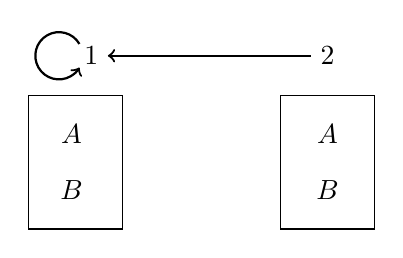
\begin{tikzpicture}
		\node (atom1) at (0,1) {1};
		\node (atom2) at (3,1) {2};
		\node (atom3) at (-0.25,0) {$A$};
		\node (atom4) at (3,0) {$\enot A$};
		\node (atom5) at (-0.25,-0.7) {$\enot B$};
		\node (atom6) at (3,-0.7) {$B$};
		\draw[->, thick] (atom1)+(-0.15,0.15) arc (-330:-30:.3);
		%\draw[->, thick] (atom2)+(0.15,-0.15) arc (-150:150:.3);
		\draw[<-, thick] (atom1) -- (atom2);
		\draw (-0.8,-1.2) rectangle (0.4,0.5);
		\draw (2.4,-1.2) rectangle (3.6,0.5);
	\end{tikzpicture}
\end{center}
Here is how to read the interpretation off from this diagram. It contains just two worlds, 1 and 2. The arrows between the worlds indicate the accessibility relation. So 1 and 2 both access 1, but neither 1 nor 2 accesses 2. The boxes at each world let us know which atomic sentences are true at each world: $A$ is true at 1 but false at 2; $B$ is false at 1 but true at 2. You may only write an atomic sentence or the negation of an atomic sentence into one of these boxes. We can figure out what truth-values the more complex sentences get at each world from that. For example, on this interpretation all of the following sentences are true at $w_1$:
\begin{itemize}
	\item[]$A\eand\enot B$, $B\eif A$, $\ediamond A$, $\ebox\enot B$
\end{itemize}
If you don't like thinking diagrammatically, then you can also present an interpretation like this:
\begin{itemize}
	\item[$W$:]$1,2$
	\item[$R$:]$\langle 1,1\rangle, \langle 2,1\rangle$
	\item[]$\nu_{1}(A)=T, \nu_{2}(B)=F, \nu_{2}(A)=F, \nu_{2}(B)=T$
\end{itemize}
You will get the chance to cook up some interpretations of your own shortly, when we start looking at \emph{counter-interpretations}.

\section{A Semantics for System \mlK}
\label{SemanticsK}

We can now extend all of the semantic concepts of TFL to cover ML:
\factoidbox{
	\begin{itemize}
		\item  $\metaX_1,\metaX_2, \dots \metaX_n\therefore\metaZ$ is \define{modally valid} iff there is no world in any interpretation at which $\metaX_1,\metaX_2, \dots \metaX_n$ are all true and $\metaZ$ is false.

		\item $\metaX$ is a \define{modal truth} iff $\metaX$ is true at every world in every interpretation.

		\item $\metaX$ is a \define{modal contradiction} iff $\metaX$ is false at every world in every interpretation.

		\item $\metaX$ is \define{modally satisfiable} iff $\metaX$ is true at some world in some interpretation.
	\end{itemize}
}
(From now on we will drop the explicit `modal' qualifications, since they can be taken as read.)

We can also extend our use of $\entails$. However, we need to add subscripts again, just as we did with $\proves$. So, when we want to say that $\metaX_1,\metaX_2, \dots \metaX_n\therefore\metaZ$ is valid, we will write: $\metaX_1,\metaX_2, \dots \metaX_n\entails_\mlK\metaZ$.

Let's get more of a feel for this semantics by presenting some counter-interpretations. Consider the following (false) claim:
\begin{itemize}
	\item[]
	      \begin{itemize}
		      \item[]$\enot A\entails_\mlK \enot \ediamond A$
	      \end{itemize}
\end{itemize}
In order to present a counter-interpretation to this claim, we need to cook up an interpretation which makes $\enot A$ true at some world $w$, and $\enot\ediamond A$ false at $w$. Here is one such interpretation, presented diagrammatically:
\begin{center}
	\begin{tikzpicture}
		\node (atom1) at (0,1) {1};
		\node (atom2) at (3,1) {2};
		\node (atom3) at (-0.25,0) {$\enot A$};
		\node (atom4) at (3,0) {$A$};
		\draw[->, thick] (atom1) -- (atom2);
		\draw (-0.8,-0.6) rectangle (0.4,0.5);
		\draw (2.4,-0.6) rectangle (3.6,0.5);
	\end{tikzpicture}
\end{center}
It is easy to see that this will work as a counter-interpretation for our claim. First, $\enot A$ is true at world $1$. And second, $\enot\ediamond A$ is false at $1$: $A$ is true at $2$, and $2$ is accessible from $1$. So there is some world in this interpretation where $\enot A$ is true and $\enot\ediamond A$ is false, so it is not the case that $\enot A\entails_\mlK\enot\ediamond A$.

Why did we choose the subscript \mlK? Well, it turns out that there is an important relationship between system \mlK{} and the definition of validity we have just given. In particular, we have the following two results:
\begin{itemize}
	\item If $\metaX_1,\metaX_2, \dots \metaX_n\proves_\mlK\metaZ$, then $\metaX_1,\metaX_2, \dots \metaX_n\entails_\mlK\metaZ$
	\item If $\metaX_1,\metaX_2, \dots \metaX_n\entails_\mlK\metaZ$, then $\metaX_1,\metaX_2, \dots \metaX_n\proves_\mlK\metaZ$
\end{itemize}
The first result is known as a \emph{soundness} result, since it tells us that the rules of \mlK{} are good, sound rules: if you can vindicate an argument by giving a proof for it using system \mlK, then that argument really is valid. The second result is known as a \emph{completeness} result, since it tells us that the rules of \mlK{} are broad enough to capture all of the valid arguments: if an argument is valid, then it will be possible to offer a proof in \mlK{} which vindicates it.

Now, it is one thing to state these results, quite another to prove them. However, we will not try to prove them here. But the idea behind the proof of soundness will perhaps make clearer how strict subproofs work.

In a strict subproof, we are not allowed to make use of any information from outside the strict subproof, except what we import into the strict subproof using \ebox E. If we've assumed or proved $\ebox \metaX$, by \ebox E, we can used $\metaX$ inside a strict subproof. And in \mlK, that is the only way to import a formula into a strict subproof. So everything that can be proved inside a strict subproof must follow from formulas $\metaX$ where outside the strict subproof we have $\ebox \metaX$. Let's imagine that we are reasoning about what's true in a possible world in some interpretation. If we know that $\ebox\metaX$ is true in that possible world, we know that $\metaX$ is true in all accessible worlds. So, everything proved inside a strict subproof is true in all accessible possible worlds. That is why \ebox I is a sound rule.

\section{A Semantics for System \mlT}
\label{SemanticsT}

A few moments ago, we said that system \mlK{} is sound and complete. Where does that leave the other modal systems we looked at, namely  \mlT, \mlSfour{} and \mlSfive? Well, they are all \emph{unsound}, relative to the definition of validity we gave above. For example, all of these systems allow us to infer $A$ from $\ebox A$, even though $\ebox A\nentails_\mlK A$.

Does that mean that these systems are a waste of time? Not at all! These systems are only unsound \emph{relative to the definition of validity we gave above}. (Or to use symbols, they are unsound relative to $\entails_\mlK$.) So when we are dealing with these stronger modal systems, we just need to modify our definition of validity to fit. This is where accessibility relations come in really handy.

When we introduced the idea of an accessibility relation, we said that it could be any relation between worlds that you like: you could have it relating every world to every world, no world to any world, or anything in between. That is how we were thinking of accessibility relations in our definition of $\entails_\mlK$. But if we wanted, we could start putting some restrictions on the accessibility relation. In particular, we might insist that it has to be \emph{reflexive}:
\begin{itemize}
	\item $\forall wRww$
\end{itemize}
In English: every world accesses itself. Or in terms of relative possibility: every world is possible relative to itself. If we imposed this restriction, we could introduce a new consequence relation, $\entails_\mlT$, as follows:
\factoidbox{
	$\metaX_1,\metaX_2, \dots \metaX_n\entails_\mlT \metaZ$ iff there is no world in any interpretation \emph{which has a reflexive accessibility relation}, at which $\metaX_1,\metaX_2, \dots \metaX_n$ are all true and $\metaZ$ is false
}
We have attached the \mlT{} subscript to $\entails$ because it turns out that system \mlT{} is sound and complete relative to this new definition of validity:
\begin{itemize}
	\item If $\metaX_1,\metaX_2, \dots \metaX_n\proves_\mlT\metaZ$, then $\metaX_1,\metaX_2, \dots \metaX_n\entails_\mlT\metaZ$
	\item If $\metaX_1,\metaX_2, \dots \metaX_n\entails_\mlT\metaZ$, then $\metaX_1,\metaX_2, \dots \metaX_n\proves_\mlT\metaZ$
\end{itemize}
As before, we will not try to prove these soundness and completeness results. However, it is relatively easy to see how insisting that the accessibility relation must be reflexive will vindicate the R\mlT{} rule:
\factoidbox{
	\[\begin{nd}
			\have[m]{m}{\ebox \metaX}
			\have[\, ]{n}{\metaX}\rt{m}
		\end{nd}\]
}
To see this, just imagine trying to cook up a counter-interpretation to this claim:
\[
	\ebox \metaX\entails_\mlT \metaX
\]
We would need to construct a world, $w$, at which $\ebox \metaX$ was true, but $\metaX$ was false. Now, if $\ebox \metaX$ is true at $w$, then $\metaX$ must be true at every world $w$ accesses. But since the accessibility relation is reflexive, $w$ accesses $w$. So $\metaX$ must be true at $w$. But now $\metaX$ must be true \emph{and} false at $w$. Contradiction!

\section{A Semantics for \mlSfour}
\label{SemanticsS4}

How else might we tweak our definition of validity? Well, we might also stipulate that the accessibility relation has to be \emph{transitive}:
\begin{itemize}
	\item $\forall w_1\forall w_2\forall w_3 ((Rw_1w_2 \eand Rw_2w_3)\eif Rw_1w_3)$
\end{itemize}
In English: if $w_1$ accesses $w_2$, and $w_2$ accesses $w_3$, then $w_1$ accesses $w_3$. Or in terms of relative possibility: if $w_3$ is possible relative to $w_2$, and $w_2$ is possible relative to $w_1$, then $w_3$ is possible relative to $w_1$. If we added this restriction on our accessibility relation, we could introduce a new consequence relation, $\entails_\mlSfour$, as follows:
\factoidbox{
	$\metaX_1,\metaX_2, \dots \metaX_n\entails_\mlSfour \metaZ$ iff there is no world in any interpretation \emph{which has a reflexive and transitive accessibility relation}, at which $\metaX_1,\metaX_2, \dots \metaX_n$ are all true and $\metaZ$ is false
}
We have attached the \mlSfour{} subscript to $\entails$ because it turns out that system \mlSfour{} is sound and complete relative to this new definition of validity:
\begin{itemize}
	\item If $\metaX_1,\metaX_2, \dots \metaX_n\proves_\mlSfour\metaZ$, then $\metaX_1,\metaX_2, \dots \metaX_n\entails_\mlSfour\metaZ$
	\item If $\metaX_1,\metaX_2, \dots \metaX_n\entails_\mlSfour\metaZ$, then $\metaX_1,\metaX_2, \dots \metaX_n\proves_\mlSfour\metaZ$
\end{itemize}
As before, we will not try to prove these soundness and completeness results. However, it is relatively easy to see how insisting that the accessibility relation must be transitive will vindicate the \mlSfour{} rule:
\factoidbox{
	\[\begin{nd}
			\have[m]{m}{\ebox\metaX}
			\open
			\hypo[\ ]{k}{\ebox}
			\have[\ ]{n}{\ebox\metaX}\rfour{m}
		\end{nd}\]
}
The idea behind strict subproofs, remember, is that they are ways to prove things that must be true in all accessible worlds. So the R$\mathbf{4}$ rule means that whenever $\ebox \metaX$ is true, $\ebox \metaX$ must also be true in every accessible world. In other words, we must have $\ebox\metaX \entails_\mlSfour \ebox\ebox\metaX$.

To see this, just imagine trying to cook up a counter-interpretation to this claim:
\begin{itemize}
	\item[]$\ebox\metaX \entails_\mlSfour \ebox \ebox \metaX$
\end{itemize}
We would need to construct a world, $w_1$, at which $\ebox\metaX$ was true, but $\ebox \ebox \metaX$ was false. Now, if $\ebox \ebox \metaX$ is false at $w_1$, then $w_1$ must access some world, $w_2$, at which $\ebox\metaX$ is false. Equally, if $\ebox \metaX$ is false at $w_2$, then $w_2$ must access some world, $w_3$, at which $\metaX$ is false. We just said that $w_1$ accesses $w_2$, and $w_2$ accesses $w_3$. So since we are now insisting that the accessibility relation be transitive, $w_1$ must access $w_3$. And as $\ebox\metaX$ is true at $w_1$, and $w_3$ is accessible from $w_1$, it follows that $\metaX$ must be true at $w_3$. So $\metaX$ is true \emph{and} false at $w_3$. Contradiction!

\section{A Semantics for \mlSfive}
\label{SemanticsS5}

Let's put one more restriction on the accessibility relation. This time, let's insist that it must also be \emph{symmetric}:
\begin{itemize}
	\item $\forall w_1\forall w_2(Rw_1w_2 \eif Rw_2w_1)$
\end{itemize}
In English: if $w_1$ accesses $w_2$, then $w_2$ accesses $w_1$. Or in terms of relative possibility: if $w_2$ is possible relative to $w_1$, then $w_1$ is possible relative to $w_2$. Logicians call a relation that is reflexive, symmetric, and transitive an \emph{equivalence} relation. We can now define a new consequence relation, $\entails_\mlSfive $, as follows:
\factoidbox{
	$\metaX_1,\metaX_2, \dots \metaX_n\entails_\mlSfive  \metaZ$ iff there is no world in any interpretation \emph{whose accessibility relation is an equivalence relation}, at which $\metaX_1,\metaX_2, \dots \metaX_n$ are all true and $\metaZ$ is false
}
We have attached the \mlSfive{} subscript to $\entails$ because it turns out that system \mlSfive{} is sound and complete relative to this new definition of validity:
\begin{itemize}
	\item If $\metaX_1,\metaX_2, \dots \metaX_n\proves_\mlSfive \metaZ$, then $\metaX_1,\metaX_2, \dots \metaX_n\entails_\mlSfive \metaZ$
	\item If $\metaX_1,\metaX_2, \dots \metaX_n\entails_\mlSfive \metaZ$, then $\metaX_1,\metaX_2, \dots \metaX_n\proves_\mlSfive \metaZ$
\end{itemize}
As before, we will not try to prove these soundness and completeness results here. However, it is relatively easy to see how insisting that the accessibility relation must be an equivalence relation will vindicate the R$\mathbf{5}$ rule:
\factoidbox{
	\[\begin{nd}
			\have[m]{m}{\enot\ebox \metaX}
			\open
			\hypo[\ ]{k}{\ebox}
			\have[\, ]{n}{\enot\ebox\metaX}\rfive{m}
		\end{nd}\]
}
The rule says that if $\metaX$ is not necessary, i.e., false in some accessible world, it is also not necessary in any accessible prossible world, i.e., we have $\enot\ebox \metaX \proves_\mlSfive  \ebox\enot\ebox \metaX$.

To see this, just imagine trying to cook up a counter-interpretation to this claim:
\[
	\enot\ebox\metaX \entails_\mlSfive  \ebox \enot\ebox \metaX
\]
We would need to construct a world, $w_1$, at which $\enot\ebox\metaX$ was true, but $\ebox \enot\ebox \metaX$ was false.
Now, if $\enot\ebox\metaX$ is true at $w_1$, then $w_1$ must access some world, $w_2$, at which $\metaX$ is false. Equally, if $\ebox \enot\ebox \metaX$ is false at $w_1$, then $w_1$ must access some world, $w_3$, at which $\enot\ebox \metaX$ is false. Since we are now insisting that the accessibility relation is an equivalence relation, and hence symmetric, we can infer that $w_3$ accesses $w_1$. Thus, $w_3$ accesses $w_1$, and $w_1$ accesses $w_2$. Again, since we are now insisting that the accessibility relation is an equivalence relation, and hence transitive, we can infer that $w_3$ accesses $w_2$. But earlier we said that $\enot\ebox \metaX$ is false at $w_3$, which implies that $\metaX$ is true at every world which $w_3$ accesses. So $\metaX$ is true \emph{and} false at $w_2$. Contradiction!

In the definition of $\entails_\mlSfive $, we stipulated that the accessibility relation must be an equivalence relation. But it turns out that there is another way of getting a notion of validity fit for \mlSfive. Rather than stipulating that the accessibility relation be an equivalence relation, we can instead stipulate that it be a \emph{universal} relation:
\begin{itemize}
	\item $\forall w_1\forall w_2Rw_1w_2$
\end{itemize}
In English: every world accesses every world. Or in terms of relative possibility: every world is possible relative to every world. Using this restriction on the accessibility relation, we could have defined $\entails_\mlSfive $ like this:
\factoidbox{
	$\metaX_1,\metaX_2, \dots \metaX_n\entails_\mlSfive  \metaZ$ iff there is no world in any interpretation \emph{which has a universal accessibility relation}, at which $\metaX_1,\metaX_2, \dots \metaX_n$ are all true and $\metaZ$ is false.
}
If we defined $\entails_\mlSfive $ like this, we would still get the same soundness and completeness results for \mlSfive. What does this tell us? Well, it means that if we are dealing with a notion of necessity according to which \emph{every} world is possible relative to \emph{every} world, then we should use \mlSfive. What is more, most philosophers assume that the notions of necessity that they are most concerned with, like \emph{logical necessity} and \emph{metaphysical necessity}, are of exactly this kind. So \mlSfive{} is the modal system that most philosophers use most of the time.

\begin{practiceproblems}

\problempart
Present counter-interpretations to the following false claims:
\begin{earg}
	\item $\enot P \entails_\mlK \enot\ediamond P$
	\item $\ebox(P \eor Q)\entails_\mlK \ebox P \eor \ebox Q$
	\item $\entails_\mlK \enot \ebox (A\eand \enot A)$
	\item $\ebox A\entails_\mlK A$
\end{earg}

\problempart
Present counter-interpretations to the following false claims:
\begin{earg}
	\item $\ediamond A\entails_\mlSfour \ebox\ediamond A$
	\item $\ediamond A, \ebox (\ediamond A \eif B)\entails_\mlSfour\ebox B$
\end{earg}

\problempart
Present counter-interpretations to the following false claims:
\begin{earg}
	\item $\ebox (M\eif O),\ediamond M\entails_\mlT O$
	\item $\ebox A\entails_\mlT \ebox \ebox A$
\end{earg}

\end{practiceproblems}

\section*{Further reading}

Modal logic is a large subfield of logic. We have only scratched the surface. If you want to learn more about modal logic, here are some textbooks you might consult.

\begin{itemize}
	\item Hughes, G. E., \& Cresswell, M. J. (1996). \emph{A New Introduction to Modal Logic}, Oxford: Routledge.
	\item Priest, G. (2008). \emph{An Introduction to Non-Classical Logic}, 2nd ed., Cambridge: Cambridge University Press.
	\item Garson, J. W. (2013). \emph{Modal Logic for Philosophers}, 2nd ed., Cambridge: Cambridge University Press.
\end{itemize}

None of these authors formulate their modal proof systems in quite the way we did, but the closest formulation is given by Garson.




\appendix
\part*{Appendices}
\addcontentsline{toc}{part}{Appendices}
\addtocontents{toc}{\protect\mbox{}\protect\hrulefill\par}

%!TEX root = forallxyyc.tex

\chapter{Symbolic notation}
\label{app.notation}

\section{Alternative nomenclature}

\paragraph{Truth-functional logic.} TFL goes by other names. Sometimes it is called \emph{sentential logic}, because it deals fundamentally with sentences. Sometimes it is called \emph{propositional logic}, on the idea that it deals fundamentally with propositions. We have stuck with \emph{truth-functional logic}, to emphasize the fact that it deals only with assignments of truth and falsity to sentences, and that its connectives are all truth-functional.

\paragraph{First-order logic.} FOL goes by other names. Sometimes it is called \emph{predicate logic}, because it allows us to apply  predicates to objects. Sometimes it is called \emph{quantified logic}, because it makes use of quantifiers.

\paragraph{Formulas.} Some texts call formulas \emph{well-formed formulas}. Since `well-formed formula' is such a long and cumbersome phrase, they then abbreviate this as \emph{wff}. This is both barbarous and unnecessary (such texts do not countenance `ill-formed formulas'). We have stuck with `formula'. 

In \S\ref{s:TFLSentences}, we defined \emph{sentences} of TFL. These are also sometimes called `formulas' (or `well-formed formulas') since in TFL, unlike FOL, there is no distinction between a formula and a sentence.

\paragraph{Valuations.} Some texts call valuations \emph{truth-assignments}, or \emph{truth-value assignments}.

\paragraph{Expressive adequacy.} Some texts describe TFL as \emph{truth-functionally complete}, rather than expressively adequate.

\paragraph{n-place predicates.} We have chosen to call predicates `one-place', `two-place', `three-place', etc. Other texts respectively call them `monadic', `dyadic', `triadic', etc. Still other texts call them `unary', `binary', `ternary', etc.

\paragraph{Names.} In FOL, we have used `$a$', `$b$', `$c$', for names. Some texts call these `constants'. Other texts do not mark any difference between names and variables in the syntax. Those texts focus simply on  whether the symbol occurs \emph{bound} or \emph{unbound}. 

\paragraph{Domains.} Some texts describe a domain as a `domain of discourse', or a `universe of discourse'.

\section{Alternative symbols}
In the history of formal logic, different symbols have been used at different times and by different authors. Often, authors were forced to use notation that their printers could typeset.

This appendix presents some common symbols, so that you can recognize them if you encounter them in an article or in another book.

\paragraph{Negation.} Two commonly used symbols are the \emph{hoe}, `$\neg$', and the \emph{swung dash} or \emph{tilda}, `${\sim}$.' In some more advanced formal systems it is necessary to distinguish between two kinds of negation; the distinction is sometimes represented by using both `$\neg$' and `${\sim}$'. Older texts sometimes indicate negation by a line over the formula being negated, e.g., $\overline{A \eand B}$. Some texts use `$x \neq y$' to abbreviate `$\enot x = y$'.

\paragraph{Disjunction.} The symbol `$\vee$' is typically used to symbolize inclusive disjunction. One etymology is from the Latin word `vel', meaning `or'.%In some systems, disjunction is written as addition.

\paragraph{Conjunction.}
Conjunction is often symbolized with the \emph{ampersand}, `{\&}'. The ampersand is a decorative form of the Latin word `et', which means `and'.  (Its etymology still lingers in certain fonts, particularly in italic fonts; thus an italic ampersand might appear as `\emph{\&}'.) This symbol is commonly used in natural English writing (e.g.  `Smith \& Sons'), and so even though it is a natural choice, many logicians use a different symbol to avoid confusion between the object and metalanguage: as a symbol in a formal system, the ampersand is not the English word `\&'. The most common choice now is `$\wedge$', which is a counterpart to the symbol used for disjunction. Sometimes a single dot, `{\scriptsize\textbullet}', is used. In some older texts, there is no symbol for conjunction at all; `$A$ and $B$' is simply written `$AB$'.

\paragraph{Material Conditional.} There are two common symbols for the material conditional: the \emph{arrow}, `$\rightarrow$', and the \emph{hook}, `$\supset$'.

\paragraph{Material Biconditional.} The \emph{double-headed arrow}, `$\leftrightarrow$', is used in systems that use the arrow to represent the material conditional. Systems that use the hook for the conditional typically use the \emph{triple bar}, `$\equiv$', for the biconditional.

\paragraph{Quantifiers.} The universal quantifier is typically symbolized as a rotated `A', and the existential quantifier as a rotated, `E'. In some texts, there is no separate symbol for the universal quantifier. Instead, the variable is just written in parentheses in front of the formula that it binds. For example, they might write `$(x)Px$' where we would write `$\forall x\, Px$'.

\bigskip

These alternative typographies are summarised below:

\begin{center}
\begin{tabular}{rl}
negation & $\neg$, ${\sim}$\\
conjunction & $\wedge$, $\&$, {\scriptsize\textbullet}\\
disjunction & $\vee$\\
conditional & $\rightarrow$, $\supset$\\
biconditional & $\leftrightarrow$, $\equiv$\\
universal quantifier & $\forall x$, $(x)$
\end{tabular}
\end{center}


%
%
%
%\section*{Polish notation}
%
%This section briefly discusses sentential logic in Polish notation, a system of notation introduced in the late 1920s by the Polish logician Jan {\L}ukasiewicz.
%
%Lower case letters are used as sentence letters. The capital letter $N$ is used for negation. $A$ is used for disjunction, $K$ for conjunction, $C$ for the conditional, $E$ for the biconditional. (`A' is for alternation, another name for logical disjunction. `E' is for equivalence.)
%%\marginpar{
%%\begin{tabular}{cc}
%%notation & Polish\\
%%of TFL & notation\\
%%\enot & $N$\\
%%\eand & $K$\\
%%\eor & $A$\\
%%\eif & $C$\\
%%\eiff & $E$
%%\end{tabular}
%%}
%
%In Polish notation, a binary connective is written \emph{before} the two sentences that it connects. For example, the sentence $A\eand B$ of TFL would be written $Kab$ in Polish notation.
%
%The sentences $\enot A\eif B$ and $\enot (A\eif B)$ are very different; the main logical operator of the first is the conditional, but the main connective of the second is negation. In TFL, we show this by putting parentheses around the conditional in the second sentence. In Polish notation, parentheses are never required. The left-most connective is always the main connective. The first sentence would simply be written $CNab$ and the second $NCab$.
%
%This feature of Polish notation means that it is possible to evaluate sentences simply by working through the symbols from right to left. If you were constructing a truth table for $NKab$, for example, you would first consider the truth-values assigned to $b$ and $a$, then consider their conjunction, and then negate the result. The general rule for what to evaluate next in TFL is not nearly so simple. In TFL, the truth table for $\enot(A\eand B)$ requires looking at $A$ and $B$, then looking in the middle of the sentence at the conjunction, and then at the beginning of the sentence at the negation. Because the order of operations can be specified more mechanically in Polish notation, variants of Polish notation are used as the internal structure for many computer programming languages.
%
 % RZ for some reason, with an \include here the TOC gets messed up
%!TEX root = forallxbris.tex

\chapter{Alternative proof systems}
In formulating our natural deduction system, we treated certain rules of natural deduction as \emph{basic}, and others as \emph{derived}. However, we could equally well have taken various different rules as basic or derived. We will illustrate this point by considering some alternative treatments of disjunction, negation, and the quantifiers. We will also explain why we have made the choices that we have.


\section{Alternative disjunction elimination}
Some systems take DS as their basic rule for disjunction elimination. Such systems can then treat the $\eor$E rule as a derived rule. For they might offer the following proof scheme: 
	\begin{fitchproof}
		\have[m]{ab}{\metaX\eor\metaY}
		\open
			\hypo[i]{a}{\metaX} {}
			\ellipsesline
			\have[j]{c1}{\meta{C}}
		\close
		\open
			\hypo[k]{b}{\metaY}{}
			\ellipsesline
			\have[l]{c2}{\meta{C}}
		\close
		\have[n]{aic}{\metaX \eif \meta{C}}\ci{a-c1}
		\have{bic}{\metaY \eif \meta{C}}\ci{b-c2}
		\have{lem}{\meta{C}\eor\enot\meta{C}}\LEM
		\open
			\hypo{c}{\meta{C}}
			\have{c1}{\meta{C}}\by{R}{c}
		\close
		\open
		\hypo{nc}{\enot \meta{C}}
		\open
			\hypo{a1}{\metaX}
			\have{c2}{\meta{C}}\ce{aic, a1}
			\have{nc1}{\ered}\ri{c2, nc}
		\close
		\have{na}{\enot\metaX}\ni{a1-nc1}
		\have{b}{\metaY}\ds{ab, na}
		\have{c3}{\meta{C}}\ce{bic, b}
	\close
	\have{con}{\meta{C}}\orE{lem,c-c1, nc-c3}
\end{fitchproof}
So why did we choose to take $\eor$E as basic, rather than DS?\footnote{P.D.\ Magnus's original version of this book went the other way.} Our reasoning is that DS involves the use of `$\enot$' in the statement of the rule. It is in some sense `cleaner' for our disjunction elimination rule to avoid mentioning \emph{other} connectives. 
The rule $\eor$E we use is also closely connected to the rule $\exists$E. Whereas there is no such analogy with DS. 


\section{Alternative negation rules}
Some systems take the following rule as their basic negation introduction rule:
\begin{fitchproof}
	\open
		\hypo[m]{a}{\metaX}
		\have[n-1]{b}{\metaY}
		\have[n]{nb}{\enot\metaY}
	\close
	\have[\ ]{}{\enot\metaX}\by{$\enot$I*}{a-nb}
\end{fitchproof}
and the following as their basic negation elimination rule:
\begin{fitchproof}
	\open
		\hypo[m]{na}{\enot\metaX}
		\have[n][-1]{b}{\metaY}
		\have{nb}{\enot\metaY}
	\close
	\have[\ ]{a}{\metaX}\by{$\enot$E*}{na-nb}
\end{fitchproof}
Using these two rules, we could have derived all of the rules governing negation and contradiction that we have taken as basic (i.e.\ $\ered$I, $\ered$E, $\enot$I and LEM). Indeed, we could have avoided all use of the symbol `$\ered$' altogether. Negation would have had a single introduction and elimination rule, and would have behaved much more like the other connectives.

The resulting system would have had fewer rules than ours. So why did we chose to separate out contradiction, and to use an explicit rule LEM?\footnote{Again, P.D.\ Magnus's original version of this book went the other way.}

Our first reason is that adding the symbol `$\ered$' to our natural deduction system makes proofs considerably easier to work with.

Our second reason is that a lot of fascinating philosophical discussion has focussed on the acceptability or otherwise of \emph{law of excluded middle} (i.e.\ LEM) and \emph{explosion} (i.e.\ $\ered$E). By treating these as separate rules in the proof system, we will be  in a better position to engage with that philosophical discussion. In particular: having invoked these rules explicitly, it will be much easier for us to know what a system which lacked these rules would look like.



\section{Alternative quantification rules}
An alternative approach to the quantifiers is to take as basic the rules for $\forall$I and $\forall$E from \S\ref{s:BasicFOL}, and also two CQ rule which allow us to move from $\forall \meta{x} \enot \metaX$ to $\enot \exists \meta{x} \metaX$ and vice versa.\footnote{Warren Goldfarb follows this line in \emph{Deductive Logic}, 2003, Hackett Publishing Co.}  

Taking only these rules as basic, we could have derived the  $\exists$I and $\exists$E rules provided in \S\ref{s:BasicFOL}. To derive the $\exists$I rule is fairly simple. Suppose $\metaX$ contains the name $\meta{c}$, and contains no instances of the variable $\meta{x}$, and that we want to do the following:
\begin{fitchproof}
	\have[m]{a}{\metaX(\ldots \meta{c} \ldots \meta{c}\ldots)}
	\have[k]{c}{\exists \meta{x} \metaX(\ldots \meta{x} \ldots \meta{c}\ldots)}
\end{fitchproof}
This is not yet permitted, since in this new system, we do not have the $\exists$I rule. We can, however, offer the following:
\begin{fitchproof}
	\hypo[m]{a}{\metaX(\ldots \meta{c} \ldots \meta{c}\ldots)}
	\open
		\hypo{nEna}{\enot \exists \meta{x} \metaX(\ldots \meta{x} \ldots \meta{c}\ldots)}
		\have{Ana}{\forall \meta{x} \enot \metaX(\ldots \meta{x} \ldots \meta{c}\ldots)}\cq{nEna}
		\have{nAc}{\enot\metaX(\ldots \meta{c} \ldots \meta{c}\ldots)}\Ae{Ana}
		\have{red}{\ered}\ri{a, nAc}
	\close
	\have{nnEa}{\enot \enot \exists \meta{x} \metaX(\ldots \meta{x} \ldots \meta{c}\ldots)}\ni{nEna-red}
	\have{end}{\exists\meta{x} \metaX(\ldots \meta{x} \ldots \meta{c}\ldots)}\dne{nnEa}
\end{fitchproof}\noindent
To derive the $\exists$E rule is rather more subtle. This is because the $\exists$E rule has an important constraint (as, indeed, does the $\forall$I rule), and we need to make sure that we are respecting it. So, suppose we are in a situation where we \emph{want} to do the following:
\begin{fitchproof}
	\have[m]{ExA}{\exists \meta{x} \metaX(\ldots \meta{x} \ldots \meta{x}\ldots)}
	\open
		\hypo[i]{Ac}{\metaX(\ldots \meta{c} \ldots \meta{c}\ldots)}
		\have[j]{B}{\metaY}
	\close
	\have[k]{end}{\metaY}
\end{fitchproof}\noindent
 where $\meta{c}$ does not occur in any undischarged assumptions, or in $\metaY$, or in $\exists \meta{x} \metaX(\ldots \meta{x} \ldots \meta{x}\ldots)$. Ordinarily, we would be allowed to use the $\exists$E rule; but we are not here assuming that we have access to this rule as a basic rule. Nevertheless, we could offer the following, more complicated derivation:
 
\begin{fitchproof}
	\have[m]{ExA}{\exists \meta{x} \metaX(\ldots \meta{x} \ldots \meta{x}\ldots)}
	\open
		\hypo[i]{Ac}{\metaX(\ldots \meta{c} \ldots \meta{c}\ldots)}
		\have[j]{B}{\metaY}
	\close
	\have[k]{condi}{\metaX(\ldots \meta{c} \ldots \meta{c}\ldots) \eif \metaY}\ci{Ac-B}
	\open
		\hypo{nB}{\enot \metaY}
		\have{nAc}{\enot \metaX(\ldots \meta{c} \ldots \meta{c}\ldots)}\mt{condi, nB}
		\have{AxnA}{\forall \meta{x} \enot \metaX(\ldots \meta{x} \ldots \meta{x}\ldots)}\by{$\forall$I}{nAc}
		\have{nEA}{\enot \exists \meta{x} \metaX(\ldots \meta{x} \ldots \meta{x}\ldots)}\cq{AxnA}
		\have{red2}{\ered}\ri{ExA, nEA}
	\close
	\have{nnB}{\enot\enot\metaY}\ni{nB-red2}
	\have{end}{\metaY}\dne{nnB}
\end{fitchproof}\noindent
We are permitted to use $\forall$I on line $k+3$ because $\meta{c}$ does not occur in any  undischarged assumptions or in $\metaY$. The entries on lines $k+4$ and $k+1$ contradict each other, because $\meta{c}$ does not occur in $\exists \meta{x} \metaX(\ldots \meta{x} \ldots \meta{x} \ldots)$.

Armed with these derived rules, we could now go on to derive the two remaining CQ rules, exactly as in \S\ref{s:DerivedFOL}.

So, why did we start with all of the quantifier rules as basic, and then derive the CQ rules? 

Our first reason is that it seems more intuitive to treat the quantifiers as on a par with one another, giving them their own basic rules for introduction and elimination. 

Our second reason relates to the discussion of alternative negation rules. In the derivations of the rules of $\exists$I and $\exists$E that we have offered in this section, we invoked DNE. This is a derived rule, whose derivation essentially depends upon the use of LEM. But, as we mentioned earlier, LEM is a contentious rule. So, if we want to move to a system which abandons LEM, but which still allows us to use existential quantifiers, we will want to take the introduction and elimination rules for the quantifiers as basic, and take the CQ rules as derived. (Indeed, in a system without LEM, we will be \emph{unable} to derive the CQ rule which moves from $\enot \forall \meta{x} \metaX$ to $\exists \meta{x} \enot \metaX$.)

%!TEX root = forallxbris.tex
\chapter{Quick reference}\label{glossary:quick ref}
%\pagestyle{plain}
\section{Sentences of TFL}
Definition of being a sentence of TFL:
	\begin{earg}
		\item Every atomic sentence is a sentence.
		\begin{itemize}
		\item $A,B,C\ldots,W$, or with subscripts $A_1, B_3, A_{100}, J_{375}$
		\end{itemize}
		\item If \metaX is a sentence, then $\enot\metaX$ is a sentence.
		\item If \metaX and \metaY are sentences, then $(\metaX\eand\metaY)$ is a sentence.
		\item If \metaX and \metaY are sentences, then $(\metaX\eor\metaY)$ is a sentence.
		\item If \metaX and \metaY are sentences, then $(\metaX\eif\metaY)$ is a sentence.
		\item If \metaX and \metaY are sentences, then $(\metaX\eiff\metaY)$ is a sentence.
		\item Nothing else is a sentence.
	\end{earg}
	
\section{Characteristic Truth Tables}
\label{app.CharacteristicTTs}

\begin{tabular}{c|c}
\metaX & \enot\metaX\\
\hline
T & F\\
F & T \\
\end{tabular}
\hfill
\begin{tabular}{c c|c|c|c|c}
\metaX & \metaY & $\metaX\eand\metaY$ & $\metaX\eor\metaY$ & $\metaX\eif\metaY$ & $\metaX\eiff\metaY$\\
\hline
T & T & T & T & T & T\\
T & F & F & T & F & F\\
F & T & F & T & T & F\\
F & F & F & F & T & T
\end{tabular}


\vfill

\section{Symbolization}
\subsubsection*{Rough Meaning of the TFL Connectives}
		\begin{tabular}{cll}
		\textbf{symbol}&\textbf{name}&\textbf{rough meaning}\\
		\hline
		\enot&negation&`It is not the case that$\ldots$'\\
		\eand&conjunction&`$\ldots$\ and $\ldots$'\\
		\eor&disjunction&`$\ldots$\ or $\ldots$'\\
		\eif&conditional&`If $\ldots$\ then $\ldots$'\\
		\eiff&biconditional&`$\ldots$ if and only if $\ldots$'\\
		\end{tabular}
		
		

\label{app.symbolization}
\subsubsection*{Sentential Connectives}
\begin{center}\begin{tabular*}{\textwidth}{ll}
It is not the case that P & $\enot P$\\
P or Q & $(P \eor Q)$\\
P and Q & $(P \eand Q)$\\
If P, then Q & $(P \eif Q)$\\
P if and only if Q & $(P \eiff Q)$\\
\end{tabular*}\end{center}Further rules:\begin{center}
\begin{tabular*}{\textwidth}{ll}
Neither P nor Q & $\enot(P \eor Q)$\ or \ $(\enot P \eand \enot Q)$\\
P but Q & $(P \eand Q)$\\
P unless Q & $(P \eor Q)$\\
P only if Q & $(P \eif Q)$
\end{tabular*}
\end{center}
\subsubsection*{Predicates}
\begin{center}
\begin{tabular*}{\textwidth}{ll}\label{SymbolizingPredicates}
All Fs are Gs & $\forall x(Fx \eif Gx)$\\
Some Fs are Gs & $\exists x(Fx \eand Gx)$\\
Not all Fs are Gs & $\enot\forall x(Fx \eif Gx)$\ or\ $\exists x(Fx \eand \enot Gx)$\\
No Fs are Gs & $\forall x(Fx \eif\enot Gx)$\ or\ $\enot\exists x(Fx \eand Gx)$\\
\end{tabular*}
\end{center}
\subsubsection*{Identity}
\begin{center}
\begin{tabular*}{\textwidth}{ll}
Only c is G & $\forall x(Gx \eif x\eid c)$ or perhaps $\eiff$.  \\
Everything besides c is G & $\forall x(\enot \,x \eid  c \eif Gx)$\\
%$j$ is more $R$ than anyone else. & $\forall x(x\neq j \eif Rjx)$\\
The F is G & $\exists x(Fx \eand \forall y(Fy \eif x\eid y) \eand Gx)$\\
It is not the case that the F is G & $\enot\exists x(Fx \eand \forall y(Fy \eif x\eid y) \eand Gx)$\\
The F is non-G & $\exists x(Fx \eand \forall y(Fy \eif x\eid y) \eand \enot Gx)$
\end{tabular*}
\end{center}






% BEGIN: symbolizing cardinality

\newpage
\section{Using identity to symbolize quantities}

\subsection*{There are at least \blank\ Fs.}
\label{summary.atleast}

\begin{ekey}
\item[\text{one}] $\exists xFx$
\item[\text{two}] $\exists x_1\exists x_2(Fx_1 \eand Fx_2 \eand \enot x_1  \eid  x_2)$
\item[\text{three}] $\exists x_1\exists x_2\exists x_3(Fx_1 \eand Fx_2 \eand Fx_3 \eand \enot x_1 \eid  x_2 \eand\enot x_1 \eid  x_3 \eand \enot x_2 \eid  x_3)$
\item[\text{four}] $\exists x_1\exists x_2\exists x_3\exists x_4 (Fx_1 \eand Fx_2 \eand Fx_3 \eand Fx_4 \eand \phantom{x}$\\
\phantom{$\exists x_1\exists x_2$}$\enot x_1 \eid  x_2 \eand \enot x_1 \eid  x_3 \eand \enot x_1 \eid  x_4 \eand \enot x_2 \eid  x_3 \eand \enot x_2 \eid  x_4 \eand \enot x_3 \eid  x_4)$
\item[n] $\exists x_1\ldots\exists x_n(Fx_1 \eand\ldots\eand Fx_n \eand \enot x_1 \eid  x_2 \eand\ldots\eand \enot x_{n-1} \eid  x_n)$ 
\end{ekey}

\subsubsection*{There are at most \blank\ Fs.}
\label{summary.atmost}

One way to say `there are at most $n$ Fs' is to put a negation sign in front of the symbolization for `there are at least $n+1$ Fs'. Equivalently, we can offer:
\begin{ekey}
\item[\text{one}] $\forall x_1\forall x_2\bigl[(Fx_1 \eand Fx_2) \eif x_1\eid x_2\bigr]$
\item[\text{two}] $\forall x_1\forall x_2\forall x_3\bigl[(Fx_1 \eand Fx_2 \eand Fx_3) \eif (x_1\eid x_2 \eor x_1\eid x_3 \eor x_2\eid x_3)\bigr]$
\item[\text{three}] $\forall x_1\forall x_2\forall x_3\forall x_4\bigl[(Fx_1 \eand Fx_2 \eand Fx_3 \eand Fx_4) \eif \phantom{.}$\\
\phantom{$\exists x_1 \exists x_2$}$(x_1\eid x_2 \eor x_1\eid x_3 \eor x_1\eid x_4 \eor x_2\eid x_3 \eor x_2\eid x_4 \eor x_3\eid x_4)\bigr]$
\item[n]$\forall x_1\ldots\forall x_{n+1}
\bigl[(Fx_1\eand \ldots \eand Fx_{n+1}) \eif (x_1\eid x_2 \eor \ldots \eor x_n\eid x_{n+1})\bigr]$ 
\end{ekey}

\subsubsection*{There are exactly \blank\ Fs.}
\label{summary.exactly}

One way to say `there are exactly $n$ Fs' is to conjoin two of the symbolizations above and say `there are at least $n$ Fs and there are at most $n$ Fs.' The following equivalent formulae are shorter:
\begin{ekey}
\item[\text{zero}] $\forall x\enot Fx$
\item[\text{one}] $\exists x\bigl[Fx \eand \forall y(Fy \eif x\eid  y)\bigr]$
\item[\text{two}] $\exists x_1\exists x_2\bigl[Fx_1 \eand Fx_2 \eand \enot x_1 \eid  x_2 \eand \forall y\bigl(Fy \eif (y\eid  x_1 \eor y \eid  x_2)\bigr) \bigr]$
\item[\text{three}] $\exists x_1\exists x_2\exists x_3\bigl[Fx_1 \eand Fx_2 \eand Fx_3 \eand \enot x_1 \eid   x_2 \eand \enot  x_1 \eid  x_3 \eand \enot x_2 \eid  x_3 \eand \phantom{.}$\\
\phantom{$\exists x_1 \exists x_2$}$\forall y\bigl(Fy \eif (y \eid  x_1 \eor y \eid  x_2 \eor y \eid   x_3)\bigr) \bigr]$
\item[n] $\exists x_1\ldots\exists x_n\bigl[Fx_1 \eand\ldots\eand Fx_n  \eand \enot x_1 \eid  x_2 \eand\ldots\eand \enot x_{n-1}\eid  x_n \eand \phantom{.}$\\
\phantom{$\exists x_1\exists x_2$}$\forall y\bigl(Fy \eif (y\eid  x_1 \eor \ldots \eor y\eid  x_n)\bigr)\bigr]$ 
%\item[one] $\exists x\forall y\bigl[Fx \eand (Fy \eif y \eid  x)\bigr]$
%\item[two] $\exists x\exists y\forall z\Bigl(Fx \eand Fy \eand \bigl[Fz \eif (z\eid x \eor z\eid y)\bigr] \eand x \neq y\Bigr)$
%\item[three] $\exists x_1\exists x_2\exists x_3\forall y\Bigl(Fx_1 \eand Fx_2 \eand Fx_3 \eand [Fy \eif (y\eid x_1 \eor y\eid x_2 \eor y\eid x_3)] \eand x_1 \neq x_2 \eand x_1 \neq x_3 \eand x_2 \neq x_3\Bigr)$
%\item[n] $\exists x_1\cdots\exists x_n\forall y\Bigl(Fx_1 \eand\cdots\eand Fx_n \eand \bigl[Fy \eif (y\eid x_1 \eor \cdots \eor y\eid x_n)\bigr] \eand x_1 \neq x_2 \eand\cdots\eand x_{n-1}\neq x_n\Bigr)$ 
\end{ekey}


\label{ProofRules}
\newpage\section{Basic deduction rules for TFL}\label{glossary:basic rules TFL}
\renewenvironment{pf}
	{\noindent\par\noindent\small$\begin{nd}}
	{\end{nd}$\noindent\normalsize\ignorespacesafterend}
	

%{\LARGE \textbf{Basic Rules of Proof}}
\begin{multicols}{2}
\subsubsection*{Reiteration}

\begin{pf}
	\have[m]{a}{\metaX}
	\have[\ ]{c}{\metaX} \by{R}{a}
\end{pf}


\subsubsection*{Conjunction}

\begin{pf}
	\have[m]{a}{\metaX}
	\have[n]{b}{\metaY}
	\have[\ ]{c}{\metaX\eand\metaY} \ai{a, b}

	\have[m]{ab}{\metaX\eand\metaY}
\\	\have[\ ]{a}{\metaX} \ae{ab}

	\have[m]{ab}{\metaX\eand\metaY}
\\	\have[\ ]{b}{\metaY} \ae{ab}
\end{pf}

\subsubsection*{Conditional}

\begin{pf}
	\open
		\hypo[m]{a}{\metaX}
		\ellipsesline
		\have[n]{b}{\metaY}
	\close
	\have[\ ]{ab}{\metaX\eif\metaY}\ci{a-b}

	\have[m]{ab}{\metaX\eif\metaY}
\\	\have[n]{a}{\metaX}
	\have[\ ]{b}{\metaY} \ce{ab,a}
\end{pf}

\subsubsection*{Biconditional}

\begin{pf}
\have[m]{ab}{\metaX\eiff\metaY}
\have[\ ]{b}{(\metaX\eif\metaY)\eand(\metaY\eif\metaX)}\iffE{ab}

\have[m]{b}{(\metaX\eif\metaY)\eand(\metaY\eif\metaX)}
\\\have[\ ]{ab}{\metaX\eiff\metaY}\iffI{b}
\end{pf}

%\begin{pf}
%	\open
%		\hypo[i]{a1}{\metaX} 
%		\have[j]{b1}{\metaY}
%	\close
%	\open
%		\hypo[k]{b2}{\metaY}
%		\have[l]{a2}{\metaX}
%	\close
%	\have[\ ]{ab}{\metaX\eiff\metaY}\bi{a1-b1,b2-a2}
%
%	\have[m]{ab}{\metaX\eiff\metaY}
%\\	\have[n]{a}{\metaX}
%	\have[\ ]{b}{\metaY} \be{ab,a}
%
%	\have[m]{ab}{\metaX\eiff\metaY}
%\\	\have[n]{a}{\metaY}
%	\have[\ ]{b}{\metaX} \be{ab,a}
%\end{pf}


\subsubsection*{Contradiction}

\begin{pf}
\have[m]{a}{\metaX}
\have[n]{na}{\enot\metaX}
\have[ ]{bot}{\ered}\ri{a, na}

\have[m]{bot}{\ered}
\\\have[ ]{}{\metaX}\re{bot}
\end{pf}


\subsubsection*{Negation}
\begin{pf}
\open
	\hypo[m]{a}{\metaX}
	\ellipsesline
	\have[n]{nb}{\ered}
\close
\have[\ ]{na}{\enot\metaX}\ni{a-nb}
\end{pf}



\subsubsection*{Disjunction}

\begin{pf}
	\have[m]{a}{\metaX}
	\have[\ ]{ab}{\metaX\eor\metaY}\oi{a}

	\have[m]{a}{\metaX}
\\	\have[\ ]{ba}{\metaY\eor\metaX}\oi{a}

	\have[m]{ab}{\metaX\eor\metaY}
\\	\open
		\hypo[i]{a}{\metaX}
		\ellipsesline
		\have[j]{c1}{\meta{C}}
	\close
	\open
		\hypo[k]{b}{\metaY}
		\ellipsesline
		\have[l]{c2}{\meta{C}}
	\close
	\have[\ ]{c}{\meta{C}} \oe{ab,a-c1, b-c2}
\end{pf}

\subsubsection*{Law of Excluded Middle}
\begin{pf}
	\have[\ ]{lem}{\metaX\eor\enot\metaX}\LEM
\end{pf}


\end{multicols}

\newpage
\section{Derived rules for TFL}
\begin{multicols}{2}
\subsubsection*{Disjunctive syllogism}
\begin{pf}
	\have[m]{ab}{\metaX \eor \metaY}
	\have[n]{nb}{\enot \metaX}
	\have[\ ]{con}{\metaY}\by{DS}{ab, nb}

	\have[m]{ab}{\metaX \eor \metaY}
\\	\have[n]{nb}{\enot \metaY}
	\have[\ ]{con}{\metaX}\by{DS}{ab, nb}
\end{pf}

%\subsubsection*{Reiteration}
%
%\begin{pf}
%	\have[m]{a}{\metaX}
%	\have[\ ]{c}{\metaX} \by{R}{a}
%\end{pf}

\subsubsection*{Modus Tollens}

\begin{pf}
	\have[m]{ab}{\metaX\eif\metaY}
	\have[n]{a}{\enot\metaY}
	\have[\ ]{b}{\enot\metaX} \by{MT}{ab,a}
\end{pf}

\subsubsection*{Double-negation elimination}
	\begin{pf}
		\have[m]{dna}{\enot \enot \metaX}
		\have[ ]{a}{\metaX}\dne{dna}
	\end{pf}


\subsubsection*{Proof by Contradiction}
	\begin{pf}
		\open
			\hypo[m]{na}{\enot\metaX}
			\ellipsesline
			\have[n]{red}{\ered}
		\close
		\have[ ]{a}{\metaX}\by{IP}{na-red}
	\end{pf}



%
%\subsubsection*{Hypothetical Syllogism}
%
%\begin{pf}
%	\have[m]{ab}{\metaX\eif\metaY}
%	\have[n]{bc}{\metaY\eif\meta{C}}
%	\have[\ ]{ac}{\metaX\eif\meta{C}}\by{HS}{ab,bc}
%\end{pf}

\subsubsection*{De Morgan Rules}
\begin{pf}
	\have[m]{ab}{\enot (\metaX \eor \metaY)}
	\have[\ ]{dm}{\enot \metaX \eand \enot \metaY}\dem{ab}

	\have[m]{ab}{\enot \metaX \eand \enot \metaY}
\\	\have[\ ]{dm}{\enot (\metaX \eor \metaY)}\dem{ab}

	\have[m]{ab}{\enot (\metaX \eand \metaY)}
\\	\have[\ ]{dm}{\enot \metaX \eor \enot \metaY}\dem{ab}

	\have[m]{ab}{\enot \metaX \eor \enot \metaY}
\\	\have[\ ]{dm}{\enot (\metaX \eand \metaY)}\dem{ab}
\end{pf}
\end{multicols}

\newpage

\section{Basic deduction rules for FOL}

\begin{multicols}{2}
\subsubsection*{Universal elimination}

\begin{pf}
	\have[m]{a}{\forall \meta{x}\metaX(\ldots \meta{x} \ldots \meta{x}\ldots)}
	\have[\ ]{c}{\metaX(\ldots \meta{c} \ldots \meta{c}\ldots)} \Ae{a}
\end{pf}

\subsubsection*{Universal introduction}

\begin{pf}
	\have[m]{a}{\metaX(\ldots \meta{c} \ldots \meta{c}\ldots)}
	\have[\ ]{c}{\forall \meta{x}\metaX(\ldots \meta{x} \ldots \meta{x}\ldots)} \Ai{a}
\end{pf}

\noindent 	\meta{c} must not occur in any undischarged assumption\\ 
\meta{x} must not occur in $\metaX(\ldots \meta{c} \ldots \meta{c}\ldots)$

%\vfill

\subsubsection*{Existential introduction}

\begin{pf}
	\have[m]{a}{\metaX(\ldots \meta{c} \ldots \meta{c}\ldots)}
	\have[\ ]{c}{\exists \meta{x}\metaX(\ldots \meta{x} \ldots \meta{c}\ldots)} \Ei{a}
\end{pf}

\noindent \meta{x} must not occur in $\metaX(\ldots \meta{c} \ldots \meta{c}\ldots)$
%\noindent You can replace one or more instance of \meta{c} with \meta{x}.

\subsubsection*{Existential elimination}

\begin{pf}
	\have[m]{a}{\exists \meta{x}\metaX(\ldots \meta{x} \ldots \meta{x}\ldots)}
	\open	
		\hypo[i]{b}{\metaX(\ldots \meta{c} \ldots \meta{c}\ldots)}
		\ellipsesline
		\have[j]{c}{\metaY}
	\close
	\have[\ ]{d}{\metaY} \Ee{a,b-c}
\end{pf}

\noindent \meta{c} must not occur in \\any undischarged assumption, \\in $\exists \meta{x}\metaX(\ldots \meta{x} \ldots \meta{x}\ldots)$, \\or in \metaY
%\vfill\columnbreak
\end{multicols}

\bigskip 

\subsubsection*{Identity introduction}

\begin{pf}
	\have[\ \,\,\,]{x}{\meta{c}\eid \meta{c}} \by{= I}{}
\end{pf}


\subsubsection*{Identity elimination}

\begin{multicols}{2}
\begin{pf}
	\have[m]{e}{\meta{a}\eid \meta{b}}
	\have[n]{a}{\metaX(\ldots \meta{a} \ldots \meta{a}\ldots)}
	\have[\ ]{ea1}{\metaX(\ldots \meta{b} \ldots \meta{a}\ldots)} \by{= E}{e,a}
\end{pf}
\begin{pf}
	\have[m]{e}{\meta{a}\eid \meta{b}}
	\have[n]{a}{\metaX(\ldots \meta{b} \ldots \meta{b}\ldots)}
	\have[\ ]{ea2}{\metaX(\ldots \meta{a} \ldots \meta{b}\ldots)} \by{= E}{e,a}
\end{pf}
\end{multicols}


\bigskip 
\section{Derived rules for FOL}
\begin{multicols}{2}
\begin{pf}
	\have[m]{ab}{\forall \meta{x}\enot \metaX}
	\have[\ ]{ac}{\enot \exists \meta{x} \metaX}\cq{m}

	\have[m]{ab}{\enot \exists \meta{x}  \metaX}
\\	\have[\ ]{ac}{\forall \meta{x}\enot\metaX}\cq{m}
\end{pf}
\begin{pf}
	\have[m]{ab}{\exists \meta{x}\enot\metaX}
	\have[\ ]{ac}{\enot \forall \meta{x} \metaX}\cq{m}

	\have[m]{ab}{\enot \forall \meta{x}  \metaX}
\\	\have[\ ]{ac}{\exists \meta{x}\enot \metaX}\cq{m}
\end{pf}
\end{multicols}



\backmatter

\glsaddallunused
\addtocontents{toc}{\protect\mbox{}\protect\hrulefill\par}
\printglossaries
%!TEX root = forallxbris.tex
\thispagestyle{empty}
\onecolumn
\ 
\vfill

\parbox{3 in}{
In the Introduction to his volume \emph{Symbolic Logic}, Charles Lutwidge Dodson advised: ``When you come to any passage you don't understand, \emph{read it again}: if you \emph{still} don't understand it, \emph{read it again}: if you fail, even after \emph{three} readings, very likely your brain is getting a little tired. In that case, put the book away, and take to other occupations, and next day, when you come to it fresh, you will very likely find that it is \emph{quite} easy.''

\medskip

The same might be said for this volume, although readers are forgiven if they take a break for snacks after \emph{two} readings.
}

\vfill

\parbox{3 in}{
%P.D.\ Magnus is an associate professor of philosophy in Albany, New York. His primary research is in the philosophy of science.

%\
%\\Tim Button is a University Lecturer, and Fellow of St John's College, at the University of Cambridge. His first book, \emph{The Limits of Realism}, was published by Oxford University Press in 2013.
}
\vfill


